\documentclass[twoside]{book}

% Packages required by doxygen
\usepackage{fixltx2e}
\usepackage{calc}
\usepackage{doxygen}
\usepackage[export]{adjustbox} % also loads graphicx
\usepackage{graphicx}
\usepackage[utf8]{inputenc}
\usepackage{makeidx}
\usepackage{multicol}
\usepackage{multirow}
\PassOptionsToPackage{warn}{textcomp}
\usepackage{textcomp}
\usepackage[nointegrals]{wasysym}
\usepackage[table]{xcolor}

% Font selection
\usepackage[T1]{fontenc}
\usepackage[scaled=.90]{helvet}
\usepackage{courier}
\usepackage{amssymb}
\usepackage{sectsty}
\renewcommand{\familydefault}{\sfdefault}
\allsectionsfont{%
  \fontseries{bc}\selectfont%
  \color{darkgray}%
}
\renewcommand{\DoxyLabelFont}{%
  \fontseries{bc}\selectfont%
  \color{darkgray}%
}
\newcommand{\+}{\discretionary{\mbox{\scriptsize$\hookleftarrow$}}{}{}}

% Page & text layout
\usepackage{geometry}
\geometry{%
  a4paper,%
  top=2.5cm,%
  bottom=2.5cm,%
  left=2.5cm,%
  right=2.5cm%
}
\tolerance=750
\hfuzz=15pt
\hbadness=750
\setlength{\emergencystretch}{15pt}
\setlength{\parindent}{0cm}
\setlength{\parskip}{0.2cm}
\makeatletter
\renewcommand{\paragraph}{%
  \@startsection{paragraph}{4}{0ex}{-1.0ex}{1.0ex}{%
    \normalfont\normalsize\bfseries\SS@parafont%
  }%
}
\renewcommand{\subparagraph}{%
  \@startsection{subparagraph}{5}{0ex}{-1.0ex}{1.0ex}{%
    \normalfont\normalsize\bfseries\SS@subparafont%
  }%
}
\makeatother

% Headers & footers
\usepackage{fancyhdr}
\pagestyle{fancyplain}
\fancyhead[LE]{\fancyplain{}{\bfseries\thepage}}
\fancyhead[CE]{\fancyplain{}{}}
\fancyhead[RE]{\fancyplain{}{\bfseries\leftmark}}
\fancyhead[LO]{\fancyplain{}{\bfseries\rightmark}}
\fancyhead[CO]{\fancyplain{}{}}
\fancyhead[RO]{\fancyplain{}{\bfseries\thepage}}
\fancyfoot[LE]{\fancyplain{}{}}
\fancyfoot[CE]{\fancyplain{}{}}
\fancyfoot[RE]{\fancyplain{}{\bfseries\scriptsize Generated on Mon Mar 23 2015 17\+:33\+:55 for Cubism\+U\+P\+\_\+2\+D by Doxygen }}
\fancyfoot[LO]{\fancyplain{}{\bfseries\scriptsize Generated on Mon Mar 23 2015 17\+:33\+:55 for Cubism\+U\+P\+\_\+2\+D by Doxygen }}
\fancyfoot[CO]{\fancyplain{}{}}
\fancyfoot[RO]{\fancyplain{}{}}
\renewcommand{\footrulewidth}{0.4pt}
\renewcommand{\chaptermark}[1]{%
  \markboth{#1}{}%
}
\renewcommand{\sectionmark}[1]{%
  \markright{\thesection\ #1}%
}

% Indices & bibliography
\usepackage{natbib}
\usepackage[titles]{tocloft}
\setcounter{tocdepth}{3}
\setcounter{secnumdepth}{5}
\makeindex

% Hyperlinks (required, but should be loaded last)
\usepackage{ifpdf}
\ifpdf
  \usepackage[pdftex,pagebackref=true]{hyperref}
\else
  \usepackage[ps2pdf,pagebackref=true]{hyperref}
\fi
\hypersetup{%
  colorlinks=true,%
  linkcolor=blue,%
  citecolor=blue,%
  unicode%
}

% Custom commands
\newcommand{\clearemptydoublepage}{%
  \newpage{\pagestyle{empty}\cleardoublepage}%
}


%===== C O N T E N T S =====

\begin{document}

% Titlepage & ToC
\hypersetup{pageanchor=false,
             bookmarks=true,
             bookmarksnumbered=true,
             pdfencoding=unicode
            }
\pagenumbering{roman}
\begin{titlepage}
\vspace*{7cm}
\begin{center}%
{\Large Cubism\+U\+P\+\_\+2\+D }\\
\vspace*{1cm}
{\large Generated by Doxygen 1.8.9.1}\\
\vspace*{0.5cm}
{\small Mon Mar 23 2015 17:33:55}\\
\end{center}
\end{titlepage}
\clearemptydoublepage
\tableofcontents
\clearemptydoublepage
\pagenumbering{arabic}
\hypersetup{pageanchor=true}

%--- Begin generated contents ---
\chapter{Namespace Index}
\section{Namespace List}
Here is a list of all namespaces with brief descriptions\+:\begin{DoxyCompactList}
\item\contentsline{section}{\hyperlink{namespace_environment}{Environment} }{\pageref{dd/dad/namespace_environment}}{}
\end{DoxyCompactList}

\chapter{Hierarchical Index}
\section{Class Hierarchy}
This inheritance list is sorted roughly, but not completely, alphabetically\+:\begin{DoxyCompactList}
\item \contentsline{section}{F\+F\+T\+W\+\_\+\+T\+Y\+P\+E\+S$<$ float $>$\+:\+:A\+L\+L\+O\+C\+A\+T\+O\+R}{\pageref{struct_f_f_t_w___t_y_p_e_s_3_01float_01_4_1_1_a_l_l_o_c_a_t_o_r}}{}
\item \contentsline{section}{F\+F\+T\+W\+\_\+\+T\+Y\+P\+E\+S$<$ double $>$\+:\+:A\+L\+L\+O\+C\+A\+T\+O\+R}{\pageref{struct_f_f_t_w___t_y_p_e_s_3_01double_01_4_1_1_a_l_l_o_c_a_t_o_r}}{}
\item \contentsline{section}{Argument\+Parser}{\pageref{class_argument_parser}}{}
\item \contentsline{section}{Block\+Info}{\pageref{struct_block_info}}{}
\item \contentsline{section}{Block\+Lab$<$ T\+Block, allocator, Element\+Type\+T $>$}{\pageref{class_block_lab}}{}
\item \contentsline{section}{Block\+Lab$<$ Block\+Type, allocator $>$}{\pageref{class_block_lab}}{}
\begin{DoxyCompactList}
\item \contentsline{section}{Block\+Lab\+Bottom\+Wall$<$ Block\+Type, allocator $>$}{\pageref{class_block_lab_bottom_wall}}{}
\item \contentsline{section}{Block\+Lab\+Box$<$ Block\+Type, allocator $>$}{\pageref{class_block_lab_box}}{}
\item \contentsline{section}{Block\+Lab\+Dirichlet$<$ Block\+Type, allocator $>$}{\pageref{class_block_lab_dirichlet}}{}
\item \contentsline{section}{Block\+Lab\+Neumann$<$ Block\+Type, allocator $>$}{\pageref{class_block_lab_neumann}}{}
\end{DoxyCompactList}
\item \contentsline{section}{Block\+Lab$<$ Block\+Type, allocator, Element\+Type\+T $>$}{\pageref{class_block_lab}}{}
\begin{DoxyCompactList}
\item \contentsline{section}{Empty\+Block\+Lab$<$ Block\+Type, allocator, Element\+Type\+T $>$}{\pageref{class_empty_block_lab}}{}
\end{DoxyCompactList}
\item \contentsline{section}{Block\+Processing\+\_\+\+T\+B\+B$<$ Block\+Type $>$}{\pageref{class_block_processing___t_b_b}}{}
\item \contentsline{section}{Block\+Processing\+M\+P\+I}{\pageref{class_block_processing_m_p_i}}{}
\item \contentsline{section}{Block\+Processing\+M\+T\+\_\+\+Simple\+\_\+\+T\+B\+B$<$ Block\+Type, Processing\+M\+T $>$}{\pageref{class_block_processing_m_t___simple___t_b_b}}{}
\item \contentsline{section}{Block\+Processing\+M\+T\+\_\+\+T\+B\+B$<$ Grid, Lab, Processing\+M\+T, n\+Slots $>$}{\pageref{class_block_processing_m_t___t_b_b}}{}
\item \contentsline{section}{Boundary\+Condition$<$ T\+Block, T\+Element, allocator $>$}{\pageref{class_boundary_condition}}{}
\item \contentsline{section}{B\+S4}{\pageref{class_b_s4}}{}
\item \contentsline{section}{Dependency\+Cube\+M\+P\+I$<$ Request $>$}{\pageref{class_dependency_cube_m_p_i}}{}
\item \contentsline{section}{Dependency\+Cube\+M\+P\+I$<$ M\+P\+I\+:\+:Request $>$}{\pageref{class_dependency_cube_m_p_i}}{}
\item \contentsline{section}{F\+F\+T\+W\+\_\+\+I\+N\+I\+T$<$ T $>$}{\pageref{struct_f_f_t_w___i_n_i_t}}{}
\item \contentsline{section}{F\+F\+T\+W\+\_\+\+I\+N\+I\+T$<$ double $>$}{\pageref{struct_f_f_t_w___i_n_i_t_3_01double_01_4}}{}
\item \contentsline{section}{F\+F\+T\+W\+\_\+\+I\+N\+I\+T$<$ float $>$}{\pageref{struct_f_f_t_w___i_n_i_t_3_01float_01_4}}{}
\item \contentsline{section}{F\+F\+T\+W\+\_\+\+T\+Y\+P\+E\+S$<$ T $>$}{\pageref{struct_f_f_t_w___t_y_p_e_s}}{}
\item \contentsline{section}{F\+F\+T\+W\+\_\+\+T\+Y\+P\+E\+S$<$ double $>$}{\pageref{struct_f_f_t_w___t_y_p_e_s_3_01double_01_4}}{}
\item \contentsline{section}{F\+F\+T\+W\+\_\+\+T\+Y\+P\+E\+S$<$ float $>$}{\pageref{struct_f_f_t_w___t_y_p_e_s_3_01float_01_4}}{}
\item \contentsline{section}{F\+F\+T\+W\+Base}{\pageref{class_f_f_t_w_base}}{}
\begin{DoxyCompactList}
\item \contentsline{section}{Poisson\+Solver\+Scalar\+F\+F\+T\+W$<$ T\+Grid, T\+Streamer $>$}{\pageref{class_poisson_solver_scalar_f_f_t_w}}{}
\begin{DoxyCompactList}
\item \contentsline{section}{Poisson\+Solver\+Vector\+F\+F\+T\+W$<$ T\+Grid, T\+Streamer $>$}{\pageref{class_poisson_solver_vector_f_f_t_w}}{}
\end{DoxyCompactList}
\end{DoxyCompactList}
\item \contentsline{section}{Fluid\+Block}{\pageref{struct_fluid_block}}{}
\item \contentsline{section}{Fluid\+Element}{\pageref{struct_fluid_element}}{}
\item \contentsline{section}{Fluid\+V\+T\+K\+Streamer}{\pageref{struct_fluid_v_t_k_streamer}}{}
\item \contentsline{section}{Generic\+Lab\+Operator}{\pageref{class_generic_lab_operator}}{}
\begin{DoxyCompactList}
\item \contentsline{section}{Operator\+Advection$<$ Remeshing\+Kernel $>$}{\pageref{class_operator_advection}}{}
\item \contentsline{section}{Operator\+Diffusion}{\pageref{class_operator_diffusion}}{}
\item \contentsline{section}{Operator\+Diffusion\+High\+Order}{\pageref{class_operator_diffusion_high_order}}{}
\item \contentsline{section}{Operator\+Divergence}{\pageref{class_operator_divergence}}{}
\item \contentsline{section}{Operator\+Divergence\+High\+Order}{\pageref{class_operator_divergence_high_order}}{}
\item \contentsline{section}{Operator\+Divergence\+Layer}{\pageref{class_operator_divergence_layer}}{}
\item \contentsline{section}{Operator\+Divergence\+Split}{\pageref{class_operator_divergence_split}}{}
\item \contentsline{section}{Operator\+Divergence\+Split\+High\+Order}{\pageref{class_operator_divergence_split_high_order}}{}
\item \contentsline{section}{Operator\+Divergence\+Split\+Layer}{\pageref{class_operator_divergence_split_layer}}{}
\item \contentsline{section}{Operator\+Grad\+P}{\pageref{class_operator_grad_p}}{}
\item \contentsline{section}{Operator\+Grad\+P\+Split}{\pageref{class_operator_grad_p_split}}{}
\item \contentsline{section}{Operator\+Grad\+P\+Split\+High\+Order}{\pageref{class_operator_grad_p_split_high_order}}{}
\item \contentsline{section}{Operator\+Split\+P}{\pageref{class_operator_split_p}}{}
\item \contentsline{section}{Operator\+Vorticity}{\pageref{class_operator_vorticity}}{}
\end{DoxyCompactList}
\item \contentsline{section}{Generic\+Operator}{\pageref{class_generic_operator}}{}
\begin{DoxyCompactList}
\item \contentsline{section}{Operator\+Compute\+Shape}{\pageref{class_operator_compute_shape}}{}
\item \contentsline{section}{Operator\+Gravity}{\pageref{class_operator_gravity}}{}
\item \contentsline{section}{Operator\+I\+C}{\pageref{class_operator_i_c}}{}
\item \contentsline{section}{Operator\+Penalization}{\pageref{class_operator_penalization}}{}
\end{DoxyCompactList}
\item \contentsline{section}{Grid$<$ Block, allocator $>$}{\pageref{class_grid}}{}
\item \contentsline{section}{Grid$<$ Block\+Type, allocator $>$}{\pageref{class_grid}}{}
\item \contentsline{section}{Indexer}{\pageref{class_indexer}}{}
\begin{DoxyCompactList}
\item \contentsline{section}{Indexer\+Morton}{\pageref{class_indexer_morton}}{}
\end{DoxyCompactList}
\item \contentsline{section}{Interface\+F\+F\+T\+W}{\pageref{class_interface_f_f_t_w}}{}
\item \contentsline{section}{Layer}{\pageref{struct_layer}}{}
\item \contentsline{section}{Matrix2\+D$<$ Data\+Type $>$}{\pageref{class_matrix2_d}}{}
\item \contentsline{section}{Matrix2\+D$<$ double $>$}{\pageref{class_matrix2_d}}{}
\item \contentsline{section}{Matrix2\+D$<$ float $>$}{\pageref{class_matrix2_d}}{}
\item \contentsline{section}{Matrix2\+D$<$ Real $>$}{\pageref{class_matrix2_d}}{}
\item \contentsline{section}{Matrix2\+D$<$ Real\mbox{[}2\mbox{]}$>$}{\pageref{class_matrix2_d}}{}
\item \contentsline{section}{Matrix3\+D$<$ Data\+Type, b\+Primitive\+Type, allocator $>$}{\pageref{class_matrix3_d}}{}
\item \contentsline{section}{Matrix3\+D$<$ Element\+Type, true, allocator $>$}{\pageref{class_matrix3_d}}{}
\item \contentsline{section}{Matrix3\+D$<$ T\+Element, true, allocator $>$}{\pageref{class_matrix3_d}}{}
\item \contentsline{section}{Matrix4\+D$<$ Data\+Type, b\+Primitive\+Type, allocator $>$}{\pageref{class_matrix4_d}}{}
\item \contentsline{section}{Metadata\+F\+F\+W\+T\+\_\+double}{\pageref{struct_metadata_f_f_w_t__double}}{}
\item \contentsline{section}{Metadata\+F\+F\+W\+T\+\_\+float}{\pageref{struct_metadata_f_f_w_t__float}}{}
\item \contentsline{section}{Mp4}{\pageref{struct_mp4}}{}
\item \contentsline{section}{Ms6}{\pageref{struct_ms6}}{}
\item \contentsline{section}{Multigrid\+Hypre}{\pageref{class_multigrid_hypre}}{}
\item My\+Block\+Lab\begin{DoxyCompactList}
\item \contentsline{section}{Block\+Lab\+M\+P\+I$<$ My\+Block\+Lab $>$}{\pageref{class_block_lab_m_p_i}}{}
\end{DoxyCompactList}
\item \contentsline{section}{Synchronizer\+M\+P\+I\+:\+:My\+Range}{\pageref{class_synchronizer_m_p_i_1_1_my_range}}{}
\item \contentsline{section}{Dependency\+Cube\+M\+P\+I$<$ Request $>$\+:\+:Object}{\pageref{struct_dependency_cube_m_p_i_1_1_object}}{}
\begin{DoxyCompactList}
\item \contentsline{section}{Dependency\+Cube\+M\+P\+I$<$ Request $>$\+:\+:Corner}{\pageref{struct_dependency_cube_m_p_i_1_1_corner}}{}
\item \contentsline{section}{Dependency\+Cube\+M\+P\+I$<$ Request $>$\+:\+:Edge}{\pageref{struct_dependency_cube_m_p_i_1_1_edge}}{}
\item \contentsline{section}{Dependency\+Cube\+M\+P\+I$<$ Request $>$\+:\+:Face}{\pageref{struct_dependency_cube_m_p_i_1_1_face}}{}
\end{DoxyCompactList}
\item \contentsline{section}{Operator\+Cut}{\pageref{class_operator_cut}}{}
\item \contentsline{section}{F\+F\+T\+W\+\_\+\+T\+Y\+P\+E\+S$<$ float $>$\+:\+:P\+L\+A\+N\+N\+E\+R}{\pageref{struct_f_f_t_w___t_y_p_e_s_3_01float_01_4_1_1_p_l_a_n_n_e_r}}{}
\item \contentsline{section}{F\+F\+T\+W\+\_\+\+T\+Y\+P\+E\+S$<$ double $>$\+:\+:P\+L\+A\+N\+N\+E\+R}{\pageref{struct_f_f_t_w___t_y_p_e_s_3_01double_01_4_1_1_p_l_a_n_n_e_r}}{}
\item \contentsline{section}{Pressure\+Solver\+\_\+\+F\+F\+T\+W}{\pageref{class_pressure_solver___f_f_t_w}}{}
\item \contentsline{section}{Profile\+Agent}{\pageref{class_profile_agent}}{}
\item \contentsline{section}{Profiler}{\pageref{class_profiler}}{}
\item \contentsline{section}{Profile\+Summary\+Item}{\pageref{struct_profile_summary_item}}{}
\item \contentsline{section}{Region}{\pageref{struct_region}}{}
\item \contentsline{section}{Serializer\+I\+O$<$ Grid\+Type, Streamer $>$}{\pageref{class_serializer_i_o}}{}
\item \contentsline{section}{Serializer\+I\+O\+\_\+\+Image\+V\+T\+K$<$ Grid\+Type, Streamer $>$}{\pageref{class_serializer_i_o___image_v_t_k}}{}
\item \contentsline{section}{Serializer\+I\+O\+\_\+\+Image\+V\+T\+K$<$ Grid, Fluid\+V\+T\+K\+Streamer $>$}{\pageref{class_serializer_i_o___image_v_t_k}}{}
\item \contentsline{section}{Serializer\+I\+O\+\_\+\+V\+P$<$ Grid\+Type, Streamer $>$}{\pageref{class_serializer_i_o___v_p}}{}
\item \contentsline{section}{Shape}{\pageref{class_shape}}{}
\begin{DoxyCompactList}
\item \contentsline{section}{Disk}{\pageref{class_disk}}{}
\item \contentsline{section}{Ellipse}{\pageref{class_ellipse}}{}
\end{DoxyCompactList}
\item \contentsline{section}{Simulation\+\_\+\+Fluid}{\pageref{class_simulation___fluid}}{}
\begin{DoxyCompactList}
\item \contentsline{section}{Simulation\+\_\+\+F\+S\+I}{\pageref{class_simulation___f_s_i}}{}
\begin{DoxyCompactList}
\item \contentsline{section}{Sim\+\_\+\+F\+S\+I\+\_\+\+Fixed}{\pageref{class_sim___f_s_i___fixed}}{}
\item \contentsline{section}{Sim\+\_\+\+F\+S\+I\+\_\+\+Gravity}{\pageref{class_sim___f_s_i___gravity}}{}
\item \contentsline{section}{Sim\+\_\+\+F\+S\+I\+\_\+\+Moving}{\pageref{class_sim___f_s_i___moving}}{}
\end{DoxyCompactList}
\end{DoxyCompactList}
\item \contentsline{section}{Stencil\+Info}{\pageref{struct_stencil_info}}{}
\item \contentsline{section}{Streamer\+Div}{\pageref{struct_streamer_div}}{}
\item \contentsline{section}{Synchronizer\+M\+P\+I}{\pageref{class_synchronizer_m_p_i}}{}
\item \contentsline{section}{Test}{\pageref{class_test}}{}
\begin{DoxyCompactList}
\item \contentsline{section}{Test\+Advection}{\pageref{class_test_advection}}{}
\item \contentsline{section}{Test\+Diffusion}{\pageref{class_test_diffusion}}{}
\item \contentsline{section}{Test\+Gravity}{\pageref{class_test_gravity}}{}
\item \contentsline{section}{Test\+Penalization}{\pageref{class_test_penalization}}{}
\item \contentsline{section}{Test\+Pressure}{\pageref{class_test_pressure}}{}
\item \contentsline{section}{Test\+Rotation}{\pageref{class_test_rotation}}{}
\item \contentsline{section}{Test\+Translation}{\pageref{class_test_translation}}{}
\item \contentsline{section}{Test\+Var\+Coeff\+Poisson}{\pageref{class_test_var_coeff_poisson}}{}
\end{DoxyCompactList}
\item T\+Grid\begin{DoxyCompactList}
\item \contentsline{section}{Grid\+Morton$<$ T\+Grid $>$}{\pageref{class_grid_morton}}{}
\item \contentsline{section}{Grid\+M\+P\+I$<$ T\+Grid $>$}{\pageref{class_grid_m_p_i}}{}
\end{DoxyCompactList}
\item \contentsline{section}{Timer}{\pageref{class_timer}}{}
\item \contentsline{section}{U\+Vfrom\+P\+S\+I\+\_\+\+S\+S\+E$<$ Real\+Type $>$}{\pageref{struct_u_vfrom_p_s_i___s_s_e}}{}
\item \contentsline{section}{U\+Vfrom\+P\+S\+I\+\_\+\+S\+S\+E$<$ double $>$}{\pageref{struct_u_vfrom_p_s_i___s_s_e_3_01double_01_4}}{}
\item \contentsline{section}{U\+Vfrom\+P\+S\+I\+\_\+\+S\+S\+E$<$ float $>$}{\pageref{struct_u_vfrom_p_s_i___s_s_e_3_01float_01_4}}{}
\item \contentsline{section}{Value}{\pageref{class_value}}{}
\item \contentsline{section}{Velocity\+Solver\+\_\+\+F\+F\+T\+W}{\pageref{class_velocity_solver___f_f_t_w}}{}
\begin{DoxyCompactList}
\item \contentsline{section}{Velocity\+Solver\+\_\+\+F\+F\+T\+W\+\_\+\+Better\+Accuracy}{\pageref{class_velocity_solver___f_f_t_w___better_accuracy}}{}
\end{DoxyCompactList}
\item \contentsline{section}{Velocity\+Solver\+\_\+\+Unbounded}{\pageref{class_velocity_solver___unbounded}}{}
\begin{DoxyCompactList}
\item \contentsline{section}{Velocity\+Solver\+\_\+\+Unbounded\+\_\+\+F\+F\+T\+W}{\pageref{class_velocity_solver___unbounded___f_f_t_w}}{}
\begin{DoxyCompactList}
\item \contentsline{section}{Pressure\+Solver\+\_\+\+Unbounded\+\_\+\+F\+F\+T\+W}{\pageref{class_pressure_solver___unbounded___f_f_t_w}}{}
\item \contentsline{section}{Velocity\+Solver\+\_\+\+Unbounded\+\_\+\+F\+F\+T\+W\+\_\+\+Better\+Accuracy}{\pageref{class_velocity_solver___unbounded___f_f_t_w___better_accuracy}}{}
\end{DoxyCompactList}
\end{DoxyCompactList}
\end{DoxyCompactList}

\chapter{Class Index}
\section{Class List}
Here are the classes, structs, unions and interfaces with brief descriptions\+:\begin{DoxyCompactList}
\item\contentsline{section}{\hyperlink{struct__header}{\+\_\+header} }{\pageref{d1/dce/struct__header}}{}
\item\contentsline{section}{\hyperlink{class_argument_parser}{Argument\+Parser} }{\pageref{d3/d52/class_argument_parser}}{}
\item\contentsline{section}{\hyperlink{struct_block_info}{Block\+Info} }{\pageref{d4/ded/struct_block_info}}{}
\item\contentsline{section}{\hyperlink{class_block_lab}{Block\+Lab$<$ T\+Block, allocator, Element\+Type\+T $>$} }{\pageref{d7/d95/class_block_lab}}{}
\item\contentsline{section}{\hyperlink{class_block_lab_bottom_wall}{Block\+Lab\+Bottom\+Wall$<$ Block\+Type, allocator $>$} }{\pageref{d1/d4e/class_block_lab_bottom_wall}}{}
\item\contentsline{section}{\hyperlink{class_block_lab_box}{Block\+Lab\+Box$<$ Block\+Type, allocator $>$} }{\pageref{db/d2b/class_block_lab_box}}{}
\item\contentsline{section}{\hyperlink{class_block_lab_dirichlet}{Block\+Lab\+Dirichlet$<$ Block\+Type, allocator $>$} }{\pageref{d6/ddf/class_block_lab_dirichlet}}{}
\item\contentsline{section}{\hyperlink{class_block_lab_m_p_i}{Block\+Lab\+M\+P\+I$<$ My\+Block\+Lab $>$} }{\pageref{d9/dee/class_block_lab_m_p_i}}{}
\item\contentsline{section}{\hyperlink{class_block_lab_neumann}{Block\+Lab\+Neumann$<$ Block\+Type, allocator $>$} }{\pageref{de/df4/class_block_lab_neumann}}{}
\item\contentsline{section}{\hyperlink{class_block_lab_pipe}{Block\+Lab\+Pipe$<$ Block\+Type, allocator $>$} }{\pageref{d0/dc2/class_block_lab_pipe}}{}
\item\contentsline{section}{\hyperlink{class_block_lab_vortex}{Block\+Lab\+Vortex$<$ Block\+Type, allocator $>$} }{\pageref{d9/dbc/class_block_lab_vortex}}{}
\item\contentsline{section}{\hyperlink{class_boundary_condition}{Boundary\+Condition$<$ T\+Block, T\+Element, allocator $>$} }{\pageref{db/d64/class_boundary_condition}}{}
\item\contentsline{section}{\hyperlink{class_b_s4}{B\+S4} }{\pageref{d3/d24/class_b_s4}}{}
\item\contentsline{section}{\hyperlink{class_coordinator_advection}{Coordinator\+Advection$<$ Lab $>$} }{\pageref{d9/d0e/class_coordinator_advection}}{}
\item\contentsline{section}{\hyperlink{class_coordinator_body_velocities}{Coordinator\+Body\+Velocities} }{\pageref{d9/ddd/class_coordinator_body_velocities}}{}
\item\contentsline{section}{\hyperlink{class_coordinator_compute_shape}{Coordinator\+Compute\+Shape} }{\pageref{d6/d6e/class_coordinator_compute_shape}}{}
\item\contentsline{section}{\hyperlink{class_coordinator_diffusion}{Coordinator\+Diffusion$<$ Lab $>$} }{\pageref{d3/dd2/class_coordinator_diffusion}}{}
\item\contentsline{section}{\hyperlink{class_coordinator_gravity}{Coordinator\+Gravity} }{\pageref{dd/dd9/class_coordinator_gravity}}{}
\item\contentsline{section}{\hyperlink{class_coordinator_i_c}{Coordinator\+I\+C} }{\pageref{da/dd2/class_coordinator_i_c}}{}
\item\contentsline{section}{\hyperlink{class_coordinator_i_c___r_t}{Coordinator\+I\+C\+\_\+\+R\+T} }{\pageref{de/d5f/class_coordinator_i_c___r_t}}{}
\item\contentsline{section}{\hyperlink{class_coordinator_penalization}{Coordinator\+Penalization} }{\pageref{d3/d93/class_coordinator_penalization}}{}
\item\contentsline{section}{\hyperlink{class_coordinator_penalization_fixed}{Coordinator\+Penalization\+Fixed} }{\pageref{d6/d40/class_coordinator_penalization_fixed}}{}
\item\contentsline{section}{\hyperlink{class_coordinator_pressure}{Coordinator\+Pressure$<$ Lab $>$} }{\pageref{df/ddf/class_coordinator_pressure}}{}
\item\contentsline{section}{\hyperlink{class_coordinator_pressure_gradient}{Coordinator\+Pressure\+Gradient} }{\pageref{d2/d29/class_coordinator_pressure_gradient}}{}
\item\contentsline{section}{\hyperlink{class_coordinator_pressure_simple}{Coordinator\+Pressure\+Simple$<$ Lab $>$} }{\pageref{d1/db7/class_coordinator_pressure_simple}}{}
\item\contentsline{section}{\hyperlink{class_coordinator_transport}{Coordinator\+Transport$<$ Lab $>$} }{\pageref{da/dda/class_coordinator_transport}}{}
\item\contentsline{section}{\hyperlink{struct_dependency_cube_m_p_i_1_1_corner}{Dependency\+Cube\+M\+P\+I$<$ Request $>$\+::\+Corner} }{\pageref{d9/d0d/struct_dependency_cube_m_p_i_1_1_corner}}{}
\item\contentsline{section}{\hyperlink{class_dependency_cube_m_p_i}{Dependency\+Cube\+M\+P\+I$<$ Request $>$} }{\pageref{d3/d21/class_dependency_cube_m_p_i}}{}
\item\contentsline{section}{\hyperlink{class_disk}{Disk} }{\pageref{d5/db6/class_disk}}{}
\item\contentsline{section}{\hyperlink{struct_dependency_cube_m_p_i_1_1_edge}{Dependency\+Cube\+M\+P\+I$<$ Request $>$\+::\+Edge} }{\pageref{df/d3d/struct_dependency_cube_m_p_i_1_1_edge}}{}
\item\contentsline{section}{\hyperlink{class_ellipse}{Ellipse} }{\pageref{dc/d25/class_ellipse}}{}
\item\contentsline{section}{\hyperlink{class_empty_block_lab}{Empty\+Block\+Lab$<$ Block\+Type, allocator, Element\+Type\+T $>$} }{\pageref{db/d11/class_empty_block_lab}}{}
\item\contentsline{section}{\hyperlink{struct_dependency_cube_m_p_i_1_1_face}{Dependency\+Cube\+M\+P\+I$<$ Request $>$\+::\+Face} }{\pageref{df/d69/struct_dependency_cube_m_p_i_1_1_face}}{}
\item\contentsline{section}{\hyperlink{class_f_f_t_w_base}{F\+F\+T\+W\+Base} }{\pageref{d3/d51/class_f_f_t_w_base}}{}
\item\contentsline{section}{\hyperlink{struct_fluid_block}{Fluid\+Block} }{\pageref{d3/ddb/struct_fluid_block}}{}
\item\contentsline{section}{\hyperlink{struct_fluid_element}{Fluid\+Element} }{\pageref{d2/d12/struct_fluid_element}}{}
\item\contentsline{section}{\hyperlink{struct_fluid_v_t_k_streamer}{Fluid\+V\+T\+K\+Streamer} }{\pageref{d8/d32/struct_fluid_v_t_k_streamer}}{}
\item\contentsline{section}{\hyperlink{class_f_p_e}{F\+P\+E$<$ T, U, mbits, ebits $>$} }{\pageref{dd/d38/class_f_p_e}}{}
\item\contentsline{section}{\hyperlink{struct_f_p_etraits}{F\+P\+Etraits$<$ T $>$} }{\pageref{da/d30/struct_f_p_etraits}}{}
\item\contentsline{section}{\hyperlink{struct_f_p_etraits_3_01double_01_4}{F\+P\+Etraits$<$ double $>$} }{\pageref{d3/d2b/struct_f_p_etraits_3_01double_01_4}}{}
\item\contentsline{section}{\hyperlink{struct_f_p_etraits_3_01float_01_4}{F\+P\+Etraits$<$ float $>$} }{\pageref{da/de7/struct_f_p_etraits_3_01float_01_4}}{}
\item\contentsline{section}{\hyperlink{class_f_r_o_n_t}{F\+R\+O\+N\+T$<$ T $>$} }{\pageref{d8/d6d/class_f_r_o_n_t}}{}
\item\contentsline{section}{\hyperlink{class_generic_coordinator}{Generic\+Coordinator} }{\pageref{d5/d8b/class_generic_coordinator}}{}
\item\contentsline{section}{\hyperlink{class_generic_lab_operator}{Generic\+Lab\+Operator} }{\pageref{dd/d3e/class_generic_lab_operator}}{}
\item\contentsline{section}{\hyperlink{class_generic_operator}{Generic\+Operator} }{\pageref{df/dbc/class_generic_operator}}{}
\item\contentsline{section}{\hyperlink{class_grid}{Grid$<$ Block, allocator $>$} }{\pageref{da/d74/class_grid}}{}
\item\contentsline{section}{\hyperlink{class_grid_morton}{Grid\+Morton$<$ T\+Grid $>$} }{\pageref{d4/db4/class_grid_morton}}{}
\item\contentsline{section}{\hyperlink{class_grid_m_p_i}{Grid\+M\+P\+I$<$ T\+Grid $>$} }{\pageref{d9/d3c/class_grid_m_p_i}}{}
\item\contentsline{section}{\hyperlink{struct_hat}{Hat} }{\pageref{df/d76/struct_hat}}{}
\item\contentsline{section}{\hyperlink{class_indexer}{Indexer} }{\pageref{d6/d1f/class_indexer}}{}
\item\contentsline{section}{\hyperlink{class_indexer_morton}{Indexer\+Morton} }{\pageref{d8/d3e/class_indexer_morton}}{}
\item\contentsline{section}{\hyperlink{struct_layer}{Layer} }{\pageref{db/dfc/struct_layer}}{}
\item\contentsline{section}{\hyperlink{class_matrix2_d}{Matrix2\+D$<$ Data\+Type $>$} }{\pageref{d2/d76/class_matrix2_d}}{}
\item\contentsline{section}{\hyperlink{class_matrix3_d}{Matrix3\+D$<$ Data\+Type, b\+Primitive\+Type, allocator $>$} }{\pageref{da/d8b/class_matrix3_d}}{}
\item\contentsline{section}{\hyperlink{class_matrix4_d}{Matrix4\+D$<$ Data\+Type, b\+Primitive\+Type, allocator $>$} }{\pageref{d6/d1d/class_matrix4_d}}{}
\item\contentsline{section}{\hyperlink{struct_mp4}{Mp4} }{\pageref{dc/db7/struct_mp4}}{}
\item\contentsline{section}{\hyperlink{struct_ms6}{Ms6} }{\pageref{db/d12/struct_ms6}}{}
\item\contentsline{section}{\hyperlink{class_multigrid_hypre}{Multigrid\+Hypre} }{\pageref{d7/d01/class_multigrid_hypre}}{}
\item\contentsline{section}{\hyperlink{class_synchronizer_m_p_i_1_1_my_range}{Synchronizer\+M\+P\+I\+::\+My\+Range} }{\pageref{d6/d85/class_synchronizer_m_p_i_1_1_my_range}}{}
\item\contentsline{section}{\hyperlink{struct_dependency_cube_m_p_i_1_1_object}{Dependency\+Cube\+M\+P\+I$<$ Request $>$\+::\+Object} }{\pageref{d2/d55/struct_dependency_cube_m_p_i_1_1_object}}{}
\item\contentsline{section}{\hyperlink{class_operator_advection}{Operator\+Advection$<$ Remeshing\+Kernel $>$} }{\pageref{df/d77/class_operator_advection}}{}
\item\contentsline{section}{\hyperlink{class_operator_advection_f_d}{Operator\+Advection\+F\+D} }{\pageref{d5/d87/class_operator_advection_f_d}}{}
\item\contentsline{section}{\hyperlink{class_operator_advection_upwind3rd_order}{Operator\+Advection\+Upwind3rd\+Order} }{\pageref{dd/d31/class_operator_advection_upwind3rd_order}}{}
\item\contentsline{section}{\hyperlink{class_operator_compute_shape}{Operator\+Compute\+Shape} }{\pageref{d1/dd9/class_operator_compute_shape}}{}
\item\contentsline{section}{\hyperlink{class_operator_diffusion}{Operator\+Diffusion} }{\pageref{d0/d55/class_operator_diffusion}}{}
\item\contentsline{section}{\hyperlink{class_operator_diffusion_high_order}{Operator\+Diffusion\+High\+Order} }{\pageref{d9/d8d/class_operator_diffusion_high_order}}{}
\item\contentsline{section}{\hyperlink{class_operator_divergence}{Operator\+Divergence} }{\pageref{d2/d52/class_operator_divergence}}{}
\item\contentsline{section}{\hyperlink{class_operator_divergence_high_order}{Operator\+Divergence\+High\+Order} }{\pageref{da/df9/class_operator_divergence_high_order}}{}
\item\contentsline{section}{\hyperlink{class_operator_divergence_layer}{Operator\+Divergence\+Layer} }{\pageref{d6/d0e/class_operator_divergence_layer}}{}
\item\contentsline{section}{\hyperlink{class_operator_divergence_split}{Operator\+Divergence\+Split} }{\pageref{d9/de4/class_operator_divergence_split}}{}
\item\contentsline{section}{\hyperlink{class_operator_divergence_split_high_order}{Operator\+Divergence\+Split\+High\+Order} }{\pageref{db/d46/class_operator_divergence_split_high_order}}{}
\item\contentsline{section}{\hyperlink{class_operator_divergence_split_layer}{Operator\+Divergence\+Split\+Layer} }{\pageref{d2/da7/class_operator_divergence_split_layer}}{}
\item\contentsline{section}{\hyperlink{class_operator_grad_p}{Operator\+Grad\+P} }{\pageref{d3/dc8/class_operator_grad_p}}{}
\item\contentsline{section}{\hyperlink{class_operator_grad_p_split}{Operator\+Grad\+P\+Split} }{\pageref{dc/d57/class_operator_grad_p_split}}{}
\item\contentsline{section}{\hyperlink{class_operator_grad_p_split_high_order}{Operator\+Grad\+P\+Split\+High\+Order} }{\pageref{dc/dc8/class_operator_grad_p_split_high_order}}{}
\item\contentsline{section}{\hyperlink{class_operator_gravity}{Operator\+Gravity} }{\pageref{d2/d34/class_operator_gravity}}{}
\item\contentsline{section}{\hyperlink{class_operator_i_c}{Operator\+I\+C} }{\pageref{de/d4a/class_operator_i_c}}{}
\item\contentsline{section}{\hyperlink{class_operator_i_c___r_t}{Operator\+I\+C\+\_\+\+R\+T} }{\pageref{d9/d03/class_operator_i_c___r_t}}{}
\item\contentsline{section}{\hyperlink{class_operator_penalization}{Operator\+Penalization} }{\pageref{df/d96/class_operator_penalization}}{}
\item\contentsline{section}{\hyperlink{class_operator_pressure_gradient}{Operator\+Pressure\+Gradient} }{\pageref{d7/d66/class_operator_pressure_gradient}}{}
\item\contentsline{section}{\hyperlink{class_operator_split_p}{Operator\+Split\+P} }{\pageref{d5/dc8/class_operator_split_p}}{}
\item\contentsline{section}{\hyperlink{class_operator_transport}{Operator\+Transport$<$ Remeshing\+Kernel $>$} }{\pageref{dc/d0c/class_operator_transport}}{}
\item\contentsline{section}{\hyperlink{class_operator_vorticity}{Operator\+Vorticity} }{\pageref{d1/d5e/class_operator_vorticity}}{}
\item\contentsline{section}{\hyperlink{class_p_cdecoder}{P\+Cdecoder$<$ T, M, wide $>$} }{\pageref{de/d92/class_p_cdecoder}}{}
\item\contentsline{section}{\hyperlink{class_p_cdecoder_3_01_t_00_01_m_00_01false_01_4}{P\+Cdecoder$<$ T, M, false $>$} }{\pageref{d9/d37/class_p_cdecoder_3_01_t_00_01_m_00_01false_01_4}}{}
\item\contentsline{section}{\hyperlink{class_p_cdecoder_3_01_t_00_01_m_00_01true_01_4}{P\+Cdecoder$<$ T, M, true $>$} }{\pageref{d8/d86/class_p_cdecoder_3_01_t_00_01_m_00_01true_01_4}}{}
\item\contentsline{section}{\hyperlink{class_p_cencoder}{P\+Cencoder$<$ T, M, wide $>$} }{\pageref{d0/dae/class_p_cencoder}}{}
\item\contentsline{section}{\hyperlink{class_p_cencoder_3_01_t_00_01_m_00_01false_01_4}{P\+Cencoder$<$ T, M, false $>$} }{\pageref{da/db3/class_p_cencoder_3_01_t_00_01_m_00_01false_01_4}}{}
\item\contentsline{section}{\hyperlink{class_p_cencoder_3_01_t_00_01_m_00_01true_01_4}{P\+Cencoder$<$ T, M, true $>$} }{\pageref{da/dac/class_p_cencoder_3_01_t_00_01_m_00_01true_01_4}}{}
\item\contentsline{section}{\hyperlink{struct_p_cmap}{P\+Cmap$<$ T, width, U $>$} }{\pageref{dd/d04/struct_p_cmap}}{}
\item\contentsline{section}{\hyperlink{struct_p_cmap_3_01double_00_01width_00_01void_01_4}{P\+Cmap$<$ double, width, void $>$} }{\pageref{df/d28/struct_p_cmap_3_01double_00_01width_00_01void_01_4}}{}
\item\contentsline{section}{\hyperlink{struct_p_cmap_3_01float_00_01width_00_01void_01_4}{P\+Cmap$<$ float, width, void $>$} }{\pageref{dc/d71/struct_p_cmap_3_01float_00_01width_00_01void_01_4}}{}
\item\contentsline{section}{\hyperlink{struct_p_cmap_3_01_t_00_01width_00_01void_01_4}{P\+Cmap$<$ T, width, void $>$} }{\pageref{dc/de9/struct_p_cmap_3_01_t_00_01width_00_01void_01_4}}{}
\item\contentsline{section}{\hyperlink{class_poisson_solver_scalar_f_f_t_w}{Poisson\+Solver\+Scalar\+F\+F\+T\+W$<$ T\+Grid, T\+Streamer $>$} }{\pageref{d3/d16/class_poisson_solver_scalar_f_f_t_w}}{}
\item\contentsline{section}{\hyperlink{class_poisson_solver_vector_f_f_t_w}{Poisson\+Solver\+Vector\+F\+F\+T\+W$<$ T\+Grid, T\+Streamer $>$} }{\pageref{d9/dfb/class_poisson_solver_vector_f_f_t_w}}{}
\item\contentsline{section}{\hyperlink{class_profile_agent}{Profile\+Agent} }{\pageref{d3/dc9/class_profile_agent}}{}
\item\contentsline{section}{\hyperlink{class_profiler}{Profiler} }{\pageref{db/db9/class_profiler}}{}
\item\contentsline{section}{\hyperlink{struct_profile_summary_item}{Profile\+Summary\+Item} }{\pageref{d5/d78/struct_profile_summary_item}}{}
\item\contentsline{section}{\hyperlink{class_r_cdecoder}{R\+Cdecoder} }{\pageref{d5/d9e/class_r_cdecoder}}{}
\item\contentsline{section}{\hyperlink{class_r_cencoder}{R\+Cencoder} }{\pageref{d5/dc7/class_r_cencoder}}{}
\item\contentsline{section}{\hyperlink{class_r_cfiledecoder}{R\+Cfiledecoder} }{\pageref{d5/d99/class_r_cfiledecoder}}{}
\item\contentsline{section}{\hyperlink{class_r_cfileencoder}{R\+Cfileencoder} }{\pageref{de/daf/class_r_cfileencoder}}{}
\item\contentsline{section}{\hyperlink{class_r_cmemdecoder}{R\+Cmemdecoder} }{\pageref{d1/df1/class_r_cmemdecoder}}{}
\item\contentsline{section}{\hyperlink{class_r_cmemencoder}{R\+Cmemencoder} }{\pageref{dc/d9e/class_r_cmemencoder}}{}
\item\contentsline{section}{\hyperlink{class_r_cmodel}{R\+Cmodel} }{\pageref{dc/d13/class_r_cmodel}}{}
\item\contentsline{section}{\hyperlink{class_r_cqsmodel}{R\+Cqsmodel} }{\pageref{d0/df1/class_r_cqsmodel}}{}
\item\contentsline{section}{\hyperlink{struct_region}{Region} }{\pageref{d4/d29/struct_region}}{}
\item\contentsline{section}{\hyperlink{class_serializer_i_o}{Serializer\+I\+O$<$ Grid\+Type, Streamer $>$} }{\pageref{d0/de5/class_serializer_i_o}}{}
\item\contentsline{section}{\hyperlink{class_serializer_i_o___image_v_t_k}{Serializer\+I\+O\+\_\+\+Image\+V\+T\+K$<$ Grid\+Type, Streamer $>$} }{\pageref{dd/d8e/class_serializer_i_o___image_v_t_k}}{}
\item\contentsline{section}{\hyperlink{class_serializer_i_o___v_p}{Serializer\+I\+O\+\_\+\+V\+P$<$ Grid\+Type, Streamer $>$} }{\pageref{d4/d3b/class_serializer_i_o___v_p}}{}
\item\contentsline{section}{\hyperlink{class_shape}{Shape} }{\pageref{d7/da7/class_shape}}{}
\item\contentsline{section}{\hyperlink{class_sim___bubble}{Sim\+\_\+\+Bubble} }{\pageref{d1/d16/class_sim___bubble}}{}
\item\contentsline{section}{\hyperlink{class_sim___f_s_i___fixed}{Sim\+\_\+\+F\+S\+I\+\_\+\+Fixed} }{\pageref{d8/d3d/class_sim___f_s_i___fixed}}{}
\item\contentsline{section}{\hyperlink{class_sim___f_s_i___gravity}{Sim\+\_\+\+F\+S\+I\+\_\+\+Gravity} }{\pageref{d6/de6/class_sim___f_s_i___gravity}}{}
\item\contentsline{section}{\hyperlink{class_sim___f_s_i___moving}{Sim\+\_\+\+F\+S\+I\+\_\+\+Moving} }{\pageref{db/df6/class_sim___f_s_i___moving}}{}
\item\contentsline{section}{\hyperlink{class_sim___jet}{Sim\+\_\+\+Jet} }{\pageref{d1/dc2/class_sim___jet}}{}
\item\contentsline{section}{\hyperlink{class_sim___rayleigh_taylor}{Sim\+\_\+\+Rayleigh\+Taylor} }{\pageref{df/d26/class_sim___rayleigh_taylor}}{}
\item\contentsline{section}{\hyperlink{class_simulation___fluid}{Simulation\+\_\+\+Fluid} }{\pageref{d0/d35/class_simulation___fluid}}{}
\item\contentsline{section}{\hyperlink{class_simulation___f_s_i}{Simulation\+\_\+\+F\+S\+I} }{\pageref{d7/dce/class_simulation___f_s_i}}{}
\item\contentsline{section}{\hyperlink{class_simulation___m_p}{Simulation\+\_\+\+M\+P} }{\pageref{de/dbd/class_simulation___m_p}}{}
\item\contentsline{section}{\hyperlink{struct_stencil_info}{Stencil\+Info} }{\pageref{da/d04/struct_stencil_info}}{}
\item\contentsline{section}{\hyperlink{struct_streamer_div}{Streamer\+Div} }{\pageref{df/df0/struct_streamer_div}}{}
\item\contentsline{section}{\hyperlink{struct_streamer_grid_point}{Streamer\+Grid\+Point} }{\pageref{de/d88/struct_streamer_grid_point}}{}
\item\contentsline{section}{\hyperlink{struct_streamer_grid_point_a_s_c_i_i}{Streamer\+Grid\+Point\+A\+S\+C\+I\+I} }{\pageref{d0/dbd/struct_streamer_grid_point_a_s_c_i_i}}{}
\item\contentsline{section}{\hyperlink{struct_streamer_serialization}{Streamer\+Serialization} }{\pageref{dd/d96/struct_streamer_serialization}}{}
\item\contentsline{section}{\hyperlink{class_synchronizer_m_p_i}{Synchronizer\+M\+P\+I} }{\pageref{d0/ddf/class_synchronizer_m_p_i}}{}
\item\contentsline{section}{\hyperlink{class_test}{Test} }{\pageref{d1/d9b/class_test}}{}
\item\contentsline{section}{\hyperlink{class_test_advection}{Test\+Advection} }{\pageref{d1/d76/class_test_advection}}{}
\item\contentsline{section}{\hyperlink{class_test_diffusion}{Test\+Diffusion} }{\pageref{d9/d0f/class_test_diffusion}}{}
\item\contentsline{section}{\hyperlink{class_test_gravity}{Test\+Gravity} }{\pageref{d2/dcc/class_test_gravity}}{}
\item\contentsline{section}{\hyperlink{class_test_penalization}{Test\+Penalization} }{\pageref{d0/d08/class_test_penalization}}{}
\item\contentsline{section}{\hyperlink{class_test_poiseuille}{Test\+Poiseuille} }{\pageref{d1/d38/class_test_poiseuille}}{}
\item\contentsline{section}{\hyperlink{class_test_pressure}{Test\+Pressure} }{\pageref{df/ddc/class_test_pressure}}{}
\item\contentsline{section}{\hyperlink{class_test_rotation}{Test\+Rotation} }{\pageref{d0/d20/class_test_rotation}}{}
\item\contentsline{section}{\hyperlink{class_test_shear_layer}{Test\+Shear\+Layer} }{\pageref{d4/d44/class_test_shear_layer}}{}
\item\contentsline{section}{\hyperlink{class_test_translation}{Test\+Translation} }{\pageref{d5/d1e/class_test_translation}}{}
\item\contentsline{section}{\hyperlink{class_test_traveling_wave}{Test\+Traveling\+Wave} }{\pageref{d1/d0e/class_test_traveling_wave}}{}
\item\contentsline{section}{\hyperlink{class_test_var_coeff_poisson}{Test\+Var\+Coeff\+Poisson} }{\pageref{d7/d0a/class_test_var_coeff_poisson}}{}
\item\contentsline{section}{\hyperlink{class_timer}{Timer} }{\pageref{d8/d08/class_timer}}{}
\item\contentsline{section}{\hyperlink{union_p_cmap_3_01float_00_01width_00_01void_01_4_1_1_u_n_i_o_n}{P\+Cmap$<$ float, width, void $>$\+::\+U\+N\+I\+O\+N} }{\pageref{de/d1a/union_p_cmap_3_01float_00_01width_00_01void_01_4_1_1_u_n_i_o_n}}{}
\item\contentsline{section}{\hyperlink{union_p_cmap_3_01double_00_01width_00_01void_01_4_1_1_u_n_i_o_n}{P\+Cmap$<$ double, width, void $>$\+::\+U\+N\+I\+O\+N} }{\pageref{df/d38/union_p_cmap_3_01double_00_01width_00_01void_01_4_1_1_u_n_i_o_n}}{}
\item\contentsline{section}{\hyperlink{class_value}{Value} }{\pageref{d4/d72/class_value}}{}
\end{DoxyCompactList}

\chapter{File Index}
\section{File List}
Here is a list of all files with brief descriptions\+:\begin{DoxyCompactList}
\item\contentsline{section}{Cubism/\hyperlink{_argument_parser_8h}{Argument\+Parser.\+h} }{\pageref{d8/d3a/_argument_parser_8h}}{}
\item\contentsline{section}{Cubism/\hyperlink{_block_info_8h}{Block\+Info.\+h} }{\pageref{d1/d07/_block_info_8h}}{}
\item\contentsline{section}{Cubism/\hyperlink{_block_lab_8h}{Block\+Lab.\+h} }{\pageref{dc/d70/_block_lab_8h}}{}
\item\contentsline{section}{Cubism/\hyperlink{_block_lab_m_p_i_8h}{Block\+Lab\+M\+P\+I.\+h} }{\pageref{d7/dce/_block_lab_m_p_i_8h}}{}
\item\contentsline{section}{Cubism/\hyperlink{_block_processing_8h}{Block\+Processing.\+h} }{\pageref{d2/ded/_block_processing_8h}}{}
\item\contentsline{section}{Cubism/\hyperlink{_block_processing_m_p_i_8h}{Block\+Processing\+M\+P\+I.\+h} }{\pageref{d8/da6/_block_processing_m_p_i_8h}}{}
\item\contentsline{section}{Cubism/\hyperlink{_dependency_cube_m_p_i_8h}{Dependency\+Cube\+M\+P\+I.\+h} }{\pageref{d9/d33/_dependency_cube_m_p_i_8h}}{}
\item\contentsline{section}{Cubism/\hyperlink{_grid_8h}{Grid.\+h} }{\pageref{d8/dea/_grid_8h}}{}
\item\contentsline{section}{Cubism/\hyperlink{_grid_morton_8h}{Grid\+Morton.\+h} }{\pageref{d7/d6b/_grid_morton_8h}}{}
\item\contentsline{section}{Cubism/\hyperlink{_grid_m_p_i_8h}{Grid\+M\+P\+I.\+h} }{\pageref{dd/d1d/_grid_m_p_i_8h}}{}
\item\contentsline{section}{Cubism/\hyperlink{_h_d_f5_dumper_8h}{H\+D\+F5\+Dumper.\+h} }{\pageref{d2/d27/_h_d_f5_dumper_8h}}{}
\item\contentsline{section}{Cubism/\hyperlink{_h_d_f5_dumper___m_p_i_8h}{H\+D\+F5\+Dumper\+\_\+\+M\+P\+I.\+h} }{\pageref{da/d42/_h_d_f5_dumper___m_p_i_8h}}{}
\item\contentsline{section}{Cubism/\hyperlink{_indexers_8h}{Indexers.\+h} }{\pageref{de/daf/_indexers_8h}}{}
\item\contentsline{section}{Cubism/\hyperlink{_matrix3_d_8h}{Matrix3\+D.\+h} }{\pageref{dd/dfa/_matrix3_d_8h}}{}
\item\contentsline{section}{Cubism/\hyperlink{_matrix4_d_8h}{Matrix4\+D.\+h} }{\pageref{dc/dc1/_matrix4_d_8h}}{}
\item\contentsline{section}{Cubism/\hyperlink{_profiler_8cpp}{Profiler.\+cpp} }{\pageref{d1/d42/_profiler_8cpp}}{}
\item\contentsline{section}{Cubism/\hyperlink{_profiler_8h}{Profiler.\+h} }{\pageref{d6/df1/_profiler_8h}}{}
\item\contentsline{section}{Cubism/\hyperlink{_p_u_pkernels_m_p_i_8h}{P\+U\+Pkernels\+M\+P\+I.\+h} }{\pageref{d7/dd2/_p_u_pkernels_m_p_i_8h}}{}
\item\contentsline{section}{Cubism/\hyperlink{_serializer_i_o_8h}{Serializer\+I\+O.\+h} }{\pageref{d7/d8f/_serializer_i_o_8h}}{}
\item\contentsline{section}{Cubism/\hyperlink{_serializer_i_o___image_v_t_k_8h}{Serializer\+I\+O\+\_\+\+Image\+V\+T\+K.\+h} }{\pageref{db/db9/_serializer_i_o___image_v_t_k_8h}}{}
\item\contentsline{section}{Cubism/\hyperlink{_serializer_i_o___v_p_8h}{Serializer\+I\+O\+\_\+\+V\+P.\+h} }{\pageref{d3/dd3/_serializer_i_o___v_p_8h}}{}
\item\contentsline{section}{Cubism/\hyperlink{_stencil_info_8h}{Stencil\+Info.\+h} }{\pageref{d4/d4e/_stencil_info_8h}}{}
\item\contentsline{section}{Cubism/\hyperlink{_synchronizer_m_p_i_8h}{Synchronizer\+M\+P\+I.\+h} }{\pageref{de/d4f/_synchronizer_m_p_i_8h}}{}
\item\contentsline{section}{Cubism/\hyperlink{_cubism_2_timer_8h}{Timer.\+h} }{\pageref{d3/df3/_cubism_2_timer_8h}}{}
\item\contentsline{section}{source/\hyperlink{_boundary_conditions_8h}{Boundary\+Conditions.\+h} }{\pageref{d5/db5/_boundary_conditions_8h}}{}
\item\contentsline{section}{source/\hyperlink{comf_8f}{comf.\+f} }{\pageref{d7/d51/comf_8f}}{}
\item\contentsline{section}{source/\hyperlink{common_8h}{common.\+h} }{\pageref{dc/d54/common_8h}}{}
\item\contentsline{section}{source/\hyperlink{_definitions_8h}{Definitions.\+h} }{\pageref{d6/d5e/_definitions_8h}}{}
\item\contentsline{section}{source/\hyperlink{genbun_8f}{genbun.\+f} }{\pageref{d6/d46/genbun_8f}}{}
\item\contentsline{section}{source/\hyperlink{_generic_operator_8h}{Generic\+Operator.\+h} }{\pageref{d2/d36/_generic_operator_8h}}{}
\item\contentsline{section}{source/\hyperlink{gnbnaux_8f}{gnbnaux.\+f} }{\pageref{d7/dd6/gnbnaux_8f}}{}
\item\contentsline{section}{source/\hyperlink{hwscrt_8f}{hwscrt.\+f} }{\pageref{d5/d81/hwscrt_8f}}{}
\item\contentsline{section}{source/\hyperlink{_interface_f_f_t_w_8h}{Interface\+F\+F\+T\+W.\+h} }{\pageref{df/ddf/_interface_f_f_t_w_8h}}{}
\item\contentsline{section}{source/\hyperlink{_interface_fortran_8h}{Interface\+Fortran.\+h} }{\pageref{d7/d17/_interface_fortran_8h}}{}
\item\contentsline{section}{source/\hyperlink{_interpolation_kernels_8h}{Interpolation\+Kernels.\+h} }{\pageref{d6/dc8/_interpolation_kernels_8h}}{}
\item\contentsline{section}{source/\hyperlink{_layer_8h}{Layer.\+h} }{\pageref{d6/d5a/_layer_8h}}{}
\item\contentsline{section}{source/\hyperlink{_layer_to_v_t_k_8h}{Layer\+To\+V\+T\+K.\+h} }{\pageref{d1/db4/_layer_to_v_t_k_8h}}{}
\item\contentsline{section}{source/\hyperlink{main_8cpp}{main.\+cpp} }{\pageref{df/d0a/main_8cpp}}{}
\item\contentsline{section}{source/\hyperlink{main_test_8cpp}{main\+Test.\+cpp} }{\pageref{dc/dd0/main_test_8cpp}}{}
\item\contentsline{section}{source/\hyperlink{_matrix2_d_8h}{Matrix2\+D.\+h} }{\pageref{dd/d66/_matrix2_d_8h}}{}
\item\contentsline{section}{source/\hyperlink{_multigrid_hypre_8h}{Multigrid\+Hypre.\+h} }{\pageref{dd/dde/_multigrid_hypre_8h}}{}
\item\contentsline{section}{source/\hyperlink{_multigrid_hypre___o_l_d_8h}{Multigrid\+Hypre\+\_\+\+O\+L\+D.\+h} }{\pageref{da/d65/_multigrid_hypre___o_l_d_8h}}{}
\item\contentsline{section}{source/\hyperlink{_operator_advection_8h}{Operator\+Advection.\+h} }{\pageref{d4/dd1/_operator_advection_8h}}{}
\item\contentsline{section}{source/\hyperlink{_operator_compute_shape_8h}{Operator\+Compute\+Shape.\+h} }{\pageref{df/d0b/_operator_compute_shape_8h}}{}
\item\contentsline{section}{source/\hyperlink{_operator_cut_8h}{Operator\+Cut.\+h} }{\pageref{df/d39/_operator_cut_8h}}{}
\item\contentsline{section}{source/\hyperlink{_operator_diffusion_8h}{Operator\+Diffusion.\+h} }{\pageref{d7/de8/_operator_diffusion_8h}}{}
\item\contentsline{section}{source/\hyperlink{_operator_divergence_8h}{Operator\+Divergence.\+h} }{\pageref{d1/ddf/_operator_divergence_8h}}{}
\item\contentsline{section}{source/\hyperlink{_operator_grad_p_8h}{Operator\+Grad\+P.\+h} }{\pageref{d0/dbd/_operator_grad_p_8h}}{}
\item\contentsline{section}{source/\hyperlink{_operator_gravity_8h}{Operator\+Gravity.\+h} }{\pageref{db/dcb/_operator_gravity_8h}}{}
\item\contentsline{section}{source/\hyperlink{_operator_i_c_8h}{Operator\+I\+C.\+h} }{\pageref{d3/d66/_operator_i_c_8h}}{}
\item\contentsline{section}{source/\hyperlink{_operator_penalization_8h}{Operator\+Penalization.\+h} }{\pageref{d1/d10/_operator_penalization_8h}}{}
\item\contentsline{section}{source/\hyperlink{_operators___d_f_t_8h}{Operators\+\_\+\+D\+F\+T.\+h} }{\pageref{d8/de0/_operators___d_f_t_8h}}{}
\item\contentsline{section}{source/\hyperlink{_operators___d_f_t___f_f_t_w_8cpp}{Operators\+\_\+\+D\+F\+T\+\_\+\+F\+F\+T\+W.\+cpp} }{\pageref{d2/d0f/_operators___d_f_t___f_f_t_w_8cpp}}{}
\item\contentsline{section}{source/\hyperlink{_operator_split_p_8h}{Operator\+Split\+P.\+h} }{\pageref{d9/dab/_operator_split_p_8h}}{}
\item\contentsline{section}{source/\hyperlink{_operator_var_coeff_poisson_8h}{Operator\+Var\+Coeff\+Poisson.\+h} }{\pageref{d2/de7/_operator_var_coeff_poisson_8h}}{}
\item\contentsline{section}{source/\hyperlink{_operator_vorticity_8h}{Operator\+Vorticity.\+h} }{\pageref{d8/db3/_operator_vorticity_8h}}{}
\item\contentsline{section}{source/\hyperlink{poisson_8f}{poisson.\+f} }{\pageref{de/dd4/poisson_8f}}{}
\item\contentsline{section}{source/\hyperlink{_poisson_solver_scalar_f_f_t_w_8cpp}{Poisson\+Solver\+Scalar\+F\+F\+T\+W.\+cpp} }{\pageref{d5/d54/_poisson_solver_scalar_f_f_t_w_8cpp}}{}
\item\contentsline{section}{source/\hyperlink{_poisson_solver_scalar_f_f_t_w_8h}{Poisson\+Solver\+Scalar\+F\+F\+T\+W.\+h} }{\pageref{d7/dc5/_poisson_solver_scalar_f_f_t_w_8h}}{}
\item\contentsline{section}{source/\hyperlink{_poisson_solver_vector_f_f_t_w_8h}{Poisson\+Solver\+Vector\+F\+F\+T\+W.\+h} }{\pageref{d6/d0b/_poisson_solver_vector_f_f_t_w_8h}}{}
\item\contentsline{section}{source/\hyperlink{_process_operators_o_m_p_8cpp}{Process\+Operators\+O\+M\+P.\+cpp} }{\pageref{d5/daa/_process_operators_o_m_p_8cpp}}{}
\item\contentsline{section}{source/\hyperlink{_process_operators_o_m_p_8h}{Process\+Operators\+O\+M\+P.\+h} }{\pageref{da/d45/_process_operators_o_m_p_8h}}{}
\item\contentsline{section}{source/\hyperlink{_shape_8h}{Shape.\+h} }{\pageref{da/d05/_shape_8h}}{}
\item\contentsline{section}{source/\hyperlink{_sim___f_s_i___fixed_8cpp}{Sim\+\_\+\+F\+S\+I\+\_\+\+Fixed.\+cpp} }{\pageref{dd/d90/_sim___f_s_i___fixed_8cpp}}{}
\item\contentsline{section}{source/\hyperlink{_sim___f_s_i___fixed_8h}{Sim\+\_\+\+F\+S\+I\+\_\+\+Fixed.\+h} }{\pageref{d3/d81/_sim___f_s_i___fixed_8h}}{}
\item\contentsline{section}{source/\hyperlink{_sim___f_s_i___gravity_8cpp}{Sim\+\_\+\+F\+S\+I\+\_\+\+Gravity.\+cpp} }{\pageref{d2/d1a/_sim___f_s_i___gravity_8cpp}}{}
\item\contentsline{section}{source/\hyperlink{_sim___f_s_i___gravity_8h}{Sim\+\_\+\+F\+S\+I\+\_\+\+Gravity.\+h} }{\pageref{d3/dfa/_sim___f_s_i___gravity_8h}}{}
\item\contentsline{section}{source/\hyperlink{_sim___f_s_i___moving_8cpp}{Sim\+\_\+\+F\+S\+I\+\_\+\+Moving.\+cpp} }{\pageref{d2/df0/_sim___f_s_i___moving_8cpp}}{}
\item\contentsline{section}{source/\hyperlink{_sim___f_s_i___moving_8h}{Sim\+\_\+\+F\+S\+I\+\_\+\+Moving.\+h} }{\pageref{d3/d92/_sim___f_s_i___moving_8h}}{}
\item\contentsline{section}{source/\hyperlink{_test_8h}{Test.\+h} }{\pageref{d6/dc0/_test_8h}}{}
\item\contentsline{section}{source/\hyperlink{_test_advection_8cpp}{Test\+Advection.\+cpp} }{\pageref{df/d7a/_test_advection_8cpp}}{}
\item\contentsline{section}{source/\hyperlink{_test_advection_8h}{Test\+Advection.\+h} }{\pageref{d3/d05/_test_advection_8h}}{}
\item\contentsline{section}{source/\hyperlink{_test_diffusion_8cpp}{Test\+Diffusion.\+cpp} }{\pageref{d4/d83/_test_diffusion_8cpp}}{}
\item\contentsline{section}{source/\hyperlink{_test_diffusion_8h}{Test\+Diffusion.\+h} }{\pageref{dc/d3e/_test_diffusion_8h}}{}
\item\contentsline{section}{source/\hyperlink{_test_gravity_8cpp}{Test\+Gravity.\+cpp} }{\pageref{d5/d42/_test_gravity_8cpp}}{}
\item\contentsline{section}{source/\hyperlink{_test_gravity_8h}{Test\+Gravity.\+h} }{\pageref{d8/df5/_test_gravity_8h}}{}
\item\contentsline{section}{source/\hyperlink{_test_penalization_8cpp}{Test\+Penalization.\+cpp} }{\pageref{dd/d7f/_test_penalization_8cpp}}{}
\item\contentsline{section}{source/\hyperlink{_test_penalization_8h}{Test\+Penalization.\+h} }{\pageref{d5/d50/_test_penalization_8h}}{}
\item\contentsline{section}{source/\hyperlink{_test_pressure_8cpp}{Test\+Pressure.\+cpp} }{\pageref{d0/df0/_test_pressure_8cpp}}{}
\item\contentsline{section}{source/\hyperlink{_test_pressure_8h}{Test\+Pressure.\+h} }{\pageref{d2/d98/_test_pressure_8h}}{}
\item\contentsline{section}{source/\hyperlink{_test_rotation_8cpp}{Test\+Rotation.\+cpp} }{\pageref{dc/def/_test_rotation_8cpp}}{}
\item\contentsline{section}{source/\hyperlink{_test_rotation_8h}{Test\+Rotation.\+h} }{\pageref{d4/d2b/_test_rotation_8h}}{}
\item\contentsline{section}{source/\hyperlink{_test_translation_8cpp}{Test\+Translation.\+cpp} }{\pageref{d5/d5f/_test_translation_8cpp}}{}
\item\contentsline{section}{source/\hyperlink{_test_translation_8h}{Test\+Translation.\+h} }{\pageref{df/d6a/_test_translation_8h}}{}
\item\contentsline{section}{source/\hyperlink{_test_var_coeff_poisson_8cpp}{Test\+Var\+Coeff\+Poisson.\+cpp} }{\pageref{de/d98/_test_var_coeff_poisson_8cpp}}{}
\item\contentsline{section}{source/\hyperlink{_test_var_coeff_poisson_8h}{Test\+Var\+Coeff\+Poisson.\+h} }{\pageref{d3/dd0/_test_var_coeff_poisson_8h}}{}
\item\contentsline{section}{source/\hyperlink{source_2_timer_8h}{Timer.\+h} }{\pageref{d3/d62/source_2_timer_8h}}{}
\end{DoxyCompactList}

\chapter{Namespace Documentation}
\hypertarget{namespace_environment}{}\section{Environment Namespace Reference}
\label{namespace_environment}\index{Environment@{Environment}}
\subsection*{Functions}
\begin{DoxyCompactItemize}
\item 
void \hyperlink{namespace_environment_ad4177ada070e3b4e16d329c30a0feb64}{setup} (int threads=-\/1)
\end{DoxyCompactItemize}


\subsection{Function Documentation}
\hypertarget{namespace_environment_ad4177ada070e3b4e16d329c30a0feb64}{}\index{Environment@{Environment}!setup@{setup}}
\index{setup@{setup}!Environment@{Environment}}
\subsubsection[{setup}]{\setlength{\rightskip}{0pt plus 5cm}void Environment\+::setup (
\begin{DoxyParamCaption}
\item[{int}]{threads = {\ttfamily -\/1}}
\end{DoxyParamCaption}
)\hspace{0.3cm}{\ttfamily [inline]}}\label{namespace_environment_ad4177ada070e3b4e16d329c30a0feb64}

\chapter{Class Documentation}
\hypertarget{struct_f_f_t_w___t_y_p_e_s_3_01float_01_4_1_1_a_l_l_o_c_a_t_o_r}{}\section{F\+F\+T\+W\+\_\+\+T\+Y\+P\+E\+S$<$ float $>$\+:\+:A\+L\+L\+O\+C\+A\+T\+O\+R Struct Reference}
\label{struct_f_f_t_w___t_y_p_e_s_3_01float_01_4_1_1_a_l_l_o_c_a_t_o_r}\index{F\+F\+T\+W\+\_\+\+T\+Y\+P\+E\+S$<$ float $>$\+::\+A\+L\+L\+O\+C\+A\+T\+O\+R@{F\+F\+T\+W\+\_\+\+T\+Y\+P\+E\+S$<$ float $>$\+::\+A\+L\+L\+O\+C\+A\+T\+O\+R}}


{\ttfamily \#include $<$Operators\+\_\+\+D\+F\+T.\+h$>$}

\subsection*{Static Public Member Functions}
\begin{DoxyCompactItemize}
\item 
{\footnotesize template$<$typename T $>$ }\\static void \hyperlink{struct_f_f_t_w___t_y_p_e_s_3_01float_01_4_1_1_a_l_l_o_c_a_t_o_r_a825d8e4a10e1eccb40d419216aeb1628}{alloc} (T $\ast$\&ptr, const int N)
\item 
{\footnotesize template$<$typename T $>$ }\\static void \hyperlink{struct_f_f_t_w___t_y_p_e_s_3_01float_01_4_1_1_a_l_l_o_c_a_t_o_r_a103673702cacc6a2a03932ca38a1916a}{free} (T $\ast$\&ptr)
\end{DoxyCompactItemize}


\subsection{Member Function Documentation}
\hypertarget{struct_f_f_t_w___t_y_p_e_s_3_01float_01_4_1_1_a_l_l_o_c_a_t_o_r_a825d8e4a10e1eccb40d419216aeb1628}{}\index{F\+F\+T\+W\+\_\+\+T\+Y\+P\+E\+S$<$ float $>$\+::\+A\+L\+L\+O\+C\+A\+T\+O\+R@{F\+F\+T\+W\+\_\+\+T\+Y\+P\+E\+S$<$ float $>$\+::\+A\+L\+L\+O\+C\+A\+T\+O\+R}!alloc@{alloc}}
\index{alloc@{alloc}!F\+F\+T\+W\+\_\+\+T\+Y\+P\+E\+S$<$ float $>$\+::\+A\+L\+L\+O\+C\+A\+T\+O\+R@{F\+F\+T\+W\+\_\+\+T\+Y\+P\+E\+S$<$ float $>$\+::\+A\+L\+L\+O\+C\+A\+T\+O\+R}}
\subsubsection[{alloc}]{\setlength{\rightskip}{0pt plus 5cm}template$<$typename T $>$ static void {\bf F\+F\+T\+W\+\_\+\+T\+Y\+P\+E\+S}$<$ float $>$\+::A\+L\+L\+O\+C\+A\+T\+O\+R\+::alloc (
\begin{DoxyParamCaption}
\item[{T $\ast$\&}]{ptr, }
\item[{const int}]{N}
\end{DoxyParamCaption}
)\hspace{0.3cm}{\ttfamily [inline]}, {\ttfamily [static]}}\label{struct_f_f_t_w___t_y_p_e_s_3_01float_01_4_1_1_a_l_l_o_c_a_t_o_r_a825d8e4a10e1eccb40d419216aeb1628}
\hypertarget{struct_f_f_t_w___t_y_p_e_s_3_01float_01_4_1_1_a_l_l_o_c_a_t_o_r_a103673702cacc6a2a03932ca38a1916a}{}\index{F\+F\+T\+W\+\_\+\+T\+Y\+P\+E\+S$<$ float $>$\+::\+A\+L\+L\+O\+C\+A\+T\+O\+R@{F\+F\+T\+W\+\_\+\+T\+Y\+P\+E\+S$<$ float $>$\+::\+A\+L\+L\+O\+C\+A\+T\+O\+R}!free@{free}}
\index{free@{free}!F\+F\+T\+W\+\_\+\+T\+Y\+P\+E\+S$<$ float $>$\+::\+A\+L\+L\+O\+C\+A\+T\+O\+R@{F\+F\+T\+W\+\_\+\+T\+Y\+P\+E\+S$<$ float $>$\+::\+A\+L\+L\+O\+C\+A\+T\+O\+R}}
\subsubsection[{free}]{\setlength{\rightskip}{0pt plus 5cm}template$<$typename T $>$ static void {\bf F\+F\+T\+W\+\_\+\+T\+Y\+P\+E\+S}$<$ float $>$\+::A\+L\+L\+O\+C\+A\+T\+O\+R\+::free (
\begin{DoxyParamCaption}
\item[{T $\ast$\&}]{ptr}
\end{DoxyParamCaption}
)\hspace{0.3cm}{\ttfamily [inline]}, {\ttfamily [static]}}\label{struct_f_f_t_w___t_y_p_e_s_3_01float_01_4_1_1_a_l_l_o_c_a_t_o_r_a103673702cacc6a2a03932ca38a1916a}


The documentation for this struct was generated from the following file\+:\begin{DoxyCompactItemize}
\item 
source/\hyperlink{_operators___d_f_t_8h}{Operators\+\_\+\+D\+F\+T.\+h}\end{DoxyCompactItemize}

\hypertarget{struct_f_f_t_w___t_y_p_e_s_3_01double_01_4_1_1_a_l_l_o_c_a_t_o_r}{}\section{F\+F\+T\+W\+\_\+\+T\+Y\+P\+E\+S$<$ double $>$\+:\+:A\+L\+L\+O\+C\+A\+T\+O\+R Struct Reference}
\label{struct_f_f_t_w___t_y_p_e_s_3_01double_01_4_1_1_a_l_l_o_c_a_t_o_r}\index{F\+F\+T\+W\+\_\+\+T\+Y\+P\+E\+S$<$ double $>$\+::\+A\+L\+L\+O\+C\+A\+T\+O\+R@{F\+F\+T\+W\+\_\+\+T\+Y\+P\+E\+S$<$ double $>$\+::\+A\+L\+L\+O\+C\+A\+T\+O\+R}}


{\ttfamily \#include $<$Operators\+\_\+\+D\+F\+T.\+h$>$}

\subsection*{Static Public Member Functions}
\begin{DoxyCompactItemize}
\item 
{\footnotesize template$<$typename T $>$ }\\static void \hyperlink{struct_f_f_t_w___t_y_p_e_s_3_01double_01_4_1_1_a_l_l_o_c_a_t_o_r_a6aa6d310b910598052c1808e955cc61d}{alloc} (T $\ast$\&ptr, const int N)
\item 
{\footnotesize template$<$typename T $>$ }\\static void \hyperlink{struct_f_f_t_w___t_y_p_e_s_3_01double_01_4_1_1_a_l_l_o_c_a_t_o_r_a11fc14281b39486977303a12df68afe4}{free} (T $\ast$\&ptr)
\end{DoxyCompactItemize}


\subsection{Member Function Documentation}
\hypertarget{struct_f_f_t_w___t_y_p_e_s_3_01double_01_4_1_1_a_l_l_o_c_a_t_o_r_a6aa6d310b910598052c1808e955cc61d}{}\index{F\+F\+T\+W\+\_\+\+T\+Y\+P\+E\+S$<$ double $>$\+::\+A\+L\+L\+O\+C\+A\+T\+O\+R@{F\+F\+T\+W\+\_\+\+T\+Y\+P\+E\+S$<$ double $>$\+::\+A\+L\+L\+O\+C\+A\+T\+O\+R}!alloc@{alloc}}
\index{alloc@{alloc}!F\+F\+T\+W\+\_\+\+T\+Y\+P\+E\+S$<$ double $>$\+::\+A\+L\+L\+O\+C\+A\+T\+O\+R@{F\+F\+T\+W\+\_\+\+T\+Y\+P\+E\+S$<$ double $>$\+::\+A\+L\+L\+O\+C\+A\+T\+O\+R}}
\subsubsection[{alloc}]{\setlength{\rightskip}{0pt plus 5cm}template$<$typename T $>$ static void {\bf F\+F\+T\+W\+\_\+\+T\+Y\+P\+E\+S}$<$ double $>$\+::A\+L\+L\+O\+C\+A\+T\+O\+R\+::alloc (
\begin{DoxyParamCaption}
\item[{T $\ast$\&}]{ptr, }
\item[{const int}]{N}
\end{DoxyParamCaption}
)\hspace{0.3cm}{\ttfamily [inline]}, {\ttfamily [static]}}\label{struct_f_f_t_w___t_y_p_e_s_3_01double_01_4_1_1_a_l_l_o_c_a_t_o_r_a6aa6d310b910598052c1808e955cc61d}
\hypertarget{struct_f_f_t_w___t_y_p_e_s_3_01double_01_4_1_1_a_l_l_o_c_a_t_o_r_a11fc14281b39486977303a12df68afe4}{}\index{F\+F\+T\+W\+\_\+\+T\+Y\+P\+E\+S$<$ double $>$\+::\+A\+L\+L\+O\+C\+A\+T\+O\+R@{F\+F\+T\+W\+\_\+\+T\+Y\+P\+E\+S$<$ double $>$\+::\+A\+L\+L\+O\+C\+A\+T\+O\+R}!free@{free}}
\index{free@{free}!F\+F\+T\+W\+\_\+\+T\+Y\+P\+E\+S$<$ double $>$\+::\+A\+L\+L\+O\+C\+A\+T\+O\+R@{F\+F\+T\+W\+\_\+\+T\+Y\+P\+E\+S$<$ double $>$\+::\+A\+L\+L\+O\+C\+A\+T\+O\+R}}
\subsubsection[{free}]{\setlength{\rightskip}{0pt plus 5cm}template$<$typename T $>$ static void {\bf F\+F\+T\+W\+\_\+\+T\+Y\+P\+E\+S}$<$ double $>$\+::A\+L\+L\+O\+C\+A\+T\+O\+R\+::free (
\begin{DoxyParamCaption}
\item[{T $\ast$\&}]{ptr}
\end{DoxyParamCaption}
)\hspace{0.3cm}{\ttfamily [inline]}, {\ttfamily [static]}}\label{struct_f_f_t_w___t_y_p_e_s_3_01double_01_4_1_1_a_l_l_o_c_a_t_o_r_a11fc14281b39486977303a12df68afe4}


The documentation for this struct was generated from the following file\+:\begin{DoxyCompactItemize}
\item 
/\+Users/cconti/\+Desktop/\+Mounts/\+Brutus\+Home/\+Seed/\+Cubism\+U\+P\+\_\+2\+D/source/\hyperlink{_operators___d_f_t_8h}{Operators\+\_\+\+D\+F\+T.\+h}\end{DoxyCompactItemize}

\hypertarget{class_argument_parser}{}\section{Argument\+Parser Class Reference}
\label{class_argument_parser}\index{Argument\+Parser@{Argument\+Parser}}


{\ttfamily \#include $<$Argument\+Parser.\+h$>$}

\subsection*{Public Member Functions}
\begin{DoxyCompactItemize}
\item 
\hyperlink{class_value}{Value} \hyperlink{class_argument_parser_acca583e2f4ed0d0eea39df89e03977ee}{operator()} (const \hyperlink{testfpzip_8cpp_a984bb8e04129c4268bd6ff36a50c9fa4}{string} arg)
\item 
bool \hyperlink{class_argument_parser_adf986abe5c47699a651ee939e198407d}{check} (const \hyperlink{testfpzip_8cpp_a984bb8e04129c4268bd6ff36a50c9fa4}{string} arg) const 
\item 
\hyperlink{class_argument_parser_a1355ae6f318c765d406d4ea600d2ea62}{Argument\+Parser} (const int argc, const char $\ast$$\ast$argv)
\item 
int \hyperlink{class_argument_parser_a778f72cb66634cea1a93446c4a0bc428}{getargc} () const 
\item 
const char $\ast$$\ast$ \hyperlink{class_argument_parser_aa20c2b84e7f77cfd65e315b8291fe342}{getargv} () const 
\item 
void \hyperlink{class_argument_parser_af30fc2364f2e0cf72e9ce17bf30fd645}{set\+\_\+strict\+\_\+mode} ()
\item 
void \hyperlink{class_argument_parser_a47b9bd39a2587221398c6785560072f8}{unset\+\_\+strict\+\_\+mode} ()
\item 
void \hyperlink{class_argument_parser_a6aaf4cd8c288d4de96aefdd5299a4f59}{mute} ()
\item 
void \hyperlink{class_argument_parser_acafcfe7dfe91ced9a020a65979bf03d9}{loud} ()
\item 
void \hyperlink{class_argument_parser_a10793f42b5c6bbb358d2929b2dc09c0f}{save\+\_\+options} (\hyperlink{testfpzip_8cpp_a984bb8e04129c4268bd6ff36a50c9fa4}{string} path=\char`\"{}.\char`\"{})
\end{DoxyCompactItemize}


\subsection{Constructor \& Destructor Documentation}
\hypertarget{class_argument_parser_a1355ae6f318c765d406d4ea600d2ea62}{}\index{Argument\+Parser@{Argument\+Parser}!Argument\+Parser@{Argument\+Parser}}
\index{Argument\+Parser@{Argument\+Parser}!Argument\+Parser@{Argument\+Parser}}
\subsubsection[{Argument\+Parser}]{\setlength{\rightskip}{0pt plus 5cm}Argument\+Parser\+::\+Argument\+Parser (
\begin{DoxyParamCaption}
\item[{const int}]{argc, }
\item[{const char $\ast$$\ast$}]{argv}
\end{DoxyParamCaption}
)\hspace{0.3cm}{\ttfamily [inline]}}\label{class_argument_parser_a1355ae6f318c765d406d4ea600d2ea62}


\subsection{Member Function Documentation}
\hypertarget{class_argument_parser_adf986abe5c47699a651ee939e198407d}{}\index{Argument\+Parser@{Argument\+Parser}!check@{check}}
\index{check@{check}!Argument\+Parser@{Argument\+Parser}}
\subsubsection[{check}]{\setlength{\rightskip}{0pt plus 5cm}bool Argument\+Parser\+::check (
\begin{DoxyParamCaption}
\item[{const {\bf string}}]{arg}
\end{DoxyParamCaption}
) const\hspace{0.3cm}{\ttfamily [inline]}}\label{class_argument_parser_adf986abe5c47699a651ee939e198407d}
\hypertarget{class_argument_parser_a778f72cb66634cea1a93446c4a0bc428}{}\index{Argument\+Parser@{Argument\+Parser}!getargc@{getargc}}
\index{getargc@{getargc}!Argument\+Parser@{Argument\+Parser}}
\subsubsection[{getargc}]{\setlength{\rightskip}{0pt plus 5cm}int Argument\+Parser\+::getargc (
\begin{DoxyParamCaption}
{}
\end{DoxyParamCaption}
) const\hspace{0.3cm}{\ttfamily [inline]}}\label{class_argument_parser_a778f72cb66634cea1a93446c4a0bc428}
\hypertarget{class_argument_parser_aa20c2b84e7f77cfd65e315b8291fe342}{}\index{Argument\+Parser@{Argument\+Parser}!getargv@{getargv}}
\index{getargv@{getargv}!Argument\+Parser@{Argument\+Parser}}
\subsubsection[{getargv}]{\setlength{\rightskip}{0pt plus 5cm}const char$\ast$$\ast$ Argument\+Parser\+::getargv (
\begin{DoxyParamCaption}
{}
\end{DoxyParamCaption}
) const\hspace{0.3cm}{\ttfamily [inline]}}\label{class_argument_parser_aa20c2b84e7f77cfd65e315b8291fe342}
\hypertarget{class_argument_parser_acafcfe7dfe91ced9a020a65979bf03d9}{}\index{Argument\+Parser@{Argument\+Parser}!loud@{loud}}
\index{loud@{loud}!Argument\+Parser@{Argument\+Parser}}
\subsubsection[{loud}]{\setlength{\rightskip}{0pt plus 5cm}void Argument\+Parser\+::loud (
\begin{DoxyParamCaption}
{}
\end{DoxyParamCaption}
)\hspace{0.3cm}{\ttfamily [inline]}}\label{class_argument_parser_acafcfe7dfe91ced9a020a65979bf03d9}
\hypertarget{class_argument_parser_a6aaf4cd8c288d4de96aefdd5299a4f59}{}\index{Argument\+Parser@{Argument\+Parser}!mute@{mute}}
\index{mute@{mute}!Argument\+Parser@{Argument\+Parser}}
\subsubsection[{mute}]{\setlength{\rightskip}{0pt plus 5cm}void Argument\+Parser\+::mute (
\begin{DoxyParamCaption}
{}
\end{DoxyParamCaption}
)\hspace{0.3cm}{\ttfamily [inline]}}\label{class_argument_parser_a6aaf4cd8c288d4de96aefdd5299a4f59}
\hypertarget{class_argument_parser_acca583e2f4ed0d0eea39df89e03977ee}{}\index{Argument\+Parser@{Argument\+Parser}!operator()@{operator()}}
\index{operator()@{operator()}!Argument\+Parser@{Argument\+Parser}}
\subsubsection[{operator()}]{\setlength{\rightskip}{0pt plus 5cm}{\bf Value} Argument\+Parser\+::operator() (
\begin{DoxyParamCaption}
\item[{const {\bf string}}]{arg}
\end{DoxyParamCaption}
)\hspace{0.3cm}{\ttfamily [inline]}}\label{class_argument_parser_acca583e2f4ed0d0eea39df89e03977ee}
\hypertarget{class_argument_parser_a10793f42b5c6bbb358d2929b2dc09c0f}{}\index{Argument\+Parser@{Argument\+Parser}!save\+\_\+options@{save\+\_\+options}}
\index{save\+\_\+options@{save\+\_\+options}!Argument\+Parser@{Argument\+Parser}}
\subsubsection[{save\+\_\+options}]{\setlength{\rightskip}{0pt plus 5cm}void Argument\+Parser\+::save\+\_\+options (
\begin{DoxyParamCaption}
\item[{{\bf string}}]{path = {\ttfamily \char`\"{}.\char`\"{}}}
\end{DoxyParamCaption}
)\hspace{0.3cm}{\ttfamily [inline]}}\label{class_argument_parser_a10793f42b5c6bbb358d2929b2dc09c0f}
\hypertarget{class_argument_parser_af30fc2364f2e0cf72e9ce17bf30fd645}{}\index{Argument\+Parser@{Argument\+Parser}!set\+\_\+strict\+\_\+mode@{set\+\_\+strict\+\_\+mode}}
\index{set\+\_\+strict\+\_\+mode@{set\+\_\+strict\+\_\+mode}!Argument\+Parser@{Argument\+Parser}}
\subsubsection[{set\+\_\+strict\+\_\+mode}]{\setlength{\rightskip}{0pt plus 5cm}void Argument\+Parser\+::set\+\_\+strict\+\_\+mode (
\begin{DoxyParamCaption}
{}
\end{DoxyParamCaption}
)\hspace{0.3cm}{\ttfamily [inline]}}\label{class_argument_parser_af30fc2364f2e0cf72e9ce17bf30fd645}


Here is the caller graph for this function\+:\nopagebreak
\begin{figure}[H]
\begin{center}
\leavevmode
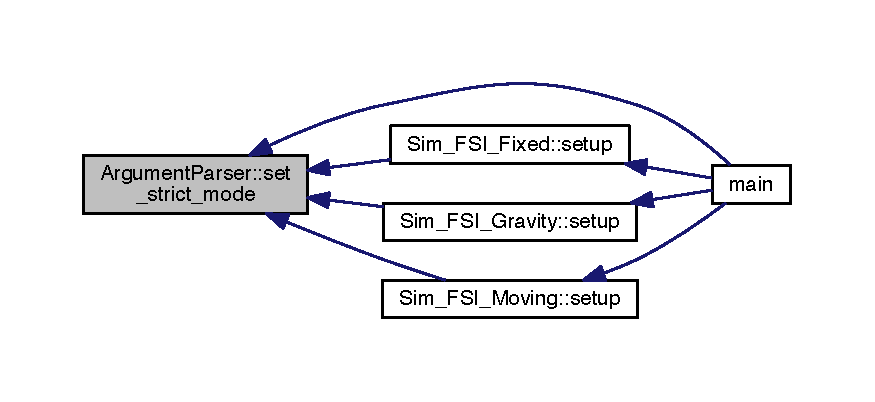
\includegraphics[width=350pt]{d3/d52/class_argument_parser_af30fc2364f2e0cf72e9ce17bf30fd645_icgraph}
\end{center}
\end{figure}


\hypertarget{class_argument_parser_a47b9bd39a2587221398c6785560072f8}{}\index{Argument\+Parser@{Argument\+Parser}!unset\+\_\+strict\+\_\+mode@{unset\+\_\+strict\+\_\+mode}}
\index{unset\+\_\+strict\+\_\+mode@{unset\+\_\+strict\+\_\+mode}!Argument\+Parser@{Argument\+Parser}}
\subsubsection[{unset\+\_\+strict\+\_\+mode}]{\setlength{\rightskip}{0pt plus 5cm}void Argument\+Parser\+::unset\+\_\+strict\+\_\+mode (
\begin{DoxyParamCaption}
{}
\end{DoxyParamCaption}
)\hspace{0.3cm}{\ttfamily [inline]}}\label{class_argument_parser_a47b9bd39a2587221398c6785560072f8}


Here is the caller graph for this function\+:\nopagebreak
\begin{figure}[H]
\begin{center}
\leavevmode
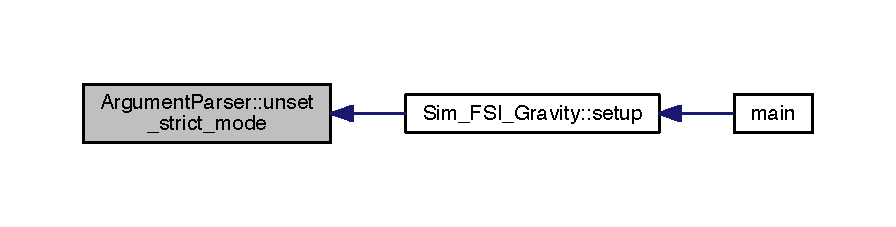
\includegraphics[width=350pt]{d3/d52/class_argument_parser_a47b9bd39a2587221398c6785560072f8_icgraph}
\end{center}
\end{figure}




The documentation for this class was generated from the following file\+:\begin{DoxyCompactItemize}
\item 
/\+Users/cconti/\+Desktop/\+Mounts/\+Brutus\+Home/\+Cubism\+U\+P\+\_\+2\+D/\+Cubism/\hyperlink{_argument_parser_8h}{Argument\+Parser.\+h}\end{DoxyCompactItemize}

\hypertarget{struct_block_info}{}\section{Block\+Info Struct Reference}
\label{struct_block_info}\index{Block\+Info@{Block\+Info}}


{\ttfamily \#include $<$Block\+Info.\+h$>$}

\subsection*{Public Member Functions}
\begin{DoxyCompactItemize}
\item 
{\footnotesize template$<$typename T $>$ }\\void \hyperlink{struct_block_info_abcc226bdb973d09286902ae23f3962fd}{pos} (T p\mbox{[}2\mbox{]}, int ix, int iy) const 
\item 
{\footnotesize template$<$typename T $>$ }\\void \hyperlink{struct_block_info_a803920cf6f3185de720fe789fa59f6cb}{pos} (T p\mbox{[}3\mbox{]}, int ix, int iy, int iz) const 
\item 
\hyperlink{struct_block_info_a02f86d450ef17d29635aa21622b641df}{Block\+Info} (long long I\+D, const int idx\mbox{[}3\mbox{]}, const double \hyperlink{struct_block_info_abcc226bdb973d09286902ae23f3962fd}{pos}\mbox{[}3\mbox{]}, const double spacing, double h\+\_\+gridpoint\+\_\+, void $\ast$ptr=N\+U\+L\+L)
\item 
\hyperlink{struct_block_info_a6b27ee44e1fa4f1b7eddb1f2e9dcaba7}{Block\+Info} ()
\end{DoxyCompactItemize}
\subsection*{Public Attributes}
\begin{DoxyCompactItemize}
\item 
long long \hyperlink{struct_block_info_aff4a50657c14cc550c9e0e3aaaed1a15}{block\+I\+D}
\item 
void $\ast$ \hyperlink{struct_block_info_af3655416c17becfb24a9f475a7b97d23}{ptr\+Block}
\item 
int \hyperlink{struct_block_info_ad32832aaa2dee35464a74abfae741572}{index} \mbox{[}3\mbox{]}
\item 
double \hyperlink{struct_block_info_a8d2d03097cfbffc58d3cc2dee371e4b2}{origin} \mbox{[}3\mbox{]}
\item 
double \hyperlink{struct_block_info_abb250cd39311bd0a840588ff2a6196ad}{h}
\item 
double \hyperlink{struct_block_info_a83bd46701539e64d666206d6501ee3ea}{h\+\_\+gridpoint}
\end{DoxyCompactItemize}


\subsection{Constructor \& Destructor Documentation}
\hypertarget{struct_block_info_a02f86d450ef17d29635aa21622b641df}{}\index{Block\+Info@{Block\+Info}!Block\+Info@{Block\+Info}}
\index{Block\+Info@{Block\+Info}!Block\+Info@{Block\+Info}}
\subsubsection[{Block\+Info}]{\setlength{\rightskip}{0pt plus 5cm}Block\+Info\+::\+Block\+Info (
\begin{DoxyParamCaption}
\item[{long long}]{I\+D, }
\item[{const int}]{idx\mbox{[}3\mbox{]}, }
\item[{const double}]{pos\mbox{[}3\mbox{]}, }
\item[{const double}]{spacing, }
\item[{double}]{h\+\_\+gridpoint\+\_\+, }
\item[{void $\ast$}]{ptr = {\ttfamily NULL}}
\end{DoxyParamCaption}
)\hspace{0.3cm}{\ttfamily [inline]}}\label{struct_block_info_a02f86d450ef17d29635aa21622b641df}
\hypertarget{struct_block_info_a6b27ee44e1fa4f1b7eddb1f2e9dcaba7}{}\index{Block\+Info@{Block\+Info}!Block\+Info@{Block\+Info}}
\index{Block\+Info@{Block\+Info}!Block\+Info@{Block\+Info}}
\subsubsection[{Block\+Info}]{\setlength{\rightskip}{0pt plus 5cm}Block\+Info\+::\+Block\+Info (
\begin{DoxyParamCaption}
{}
\end{DoxyParamCaption}
)\hspace{0.3cm}{\ttfamily [inline]}}\label{struct_block_info_a6b27ee44e1fa4f1b7eddb1f2e9dcaba7}


\subsection{Member Function Documentation}
\hypertarget{struct_block_info_abcc226bdb973d09286902ae23f3962fd}{}\index{Block\+Info@{Block\+Info}!pos@{pos}}
\index{pos@{pos}!Block\+Info@{Block\+Info}}
\subsubsection[{pos}]{\setlength{\rightskip}{0pt plus 5cm}template$<$typename T $>$ void Block\+Info\+::pos (
\begin{DoxyParamCaption}
\item[{T}]{p\mbox{[}2\mbox{]}, }
\item[{int}]{ix, }
\item[{int}]{iy}
\end{DoxyParamCaption}
) const\hspace{0.3cm}{\ttfamily [inline]}}\label{struct_block_info_abcc226bdb973d09286902ae23f3962fd}


Here is the caller graph for this function\+:
\nopagebreak
\begin{figure}[H]
\begin{center}
\leavevmode
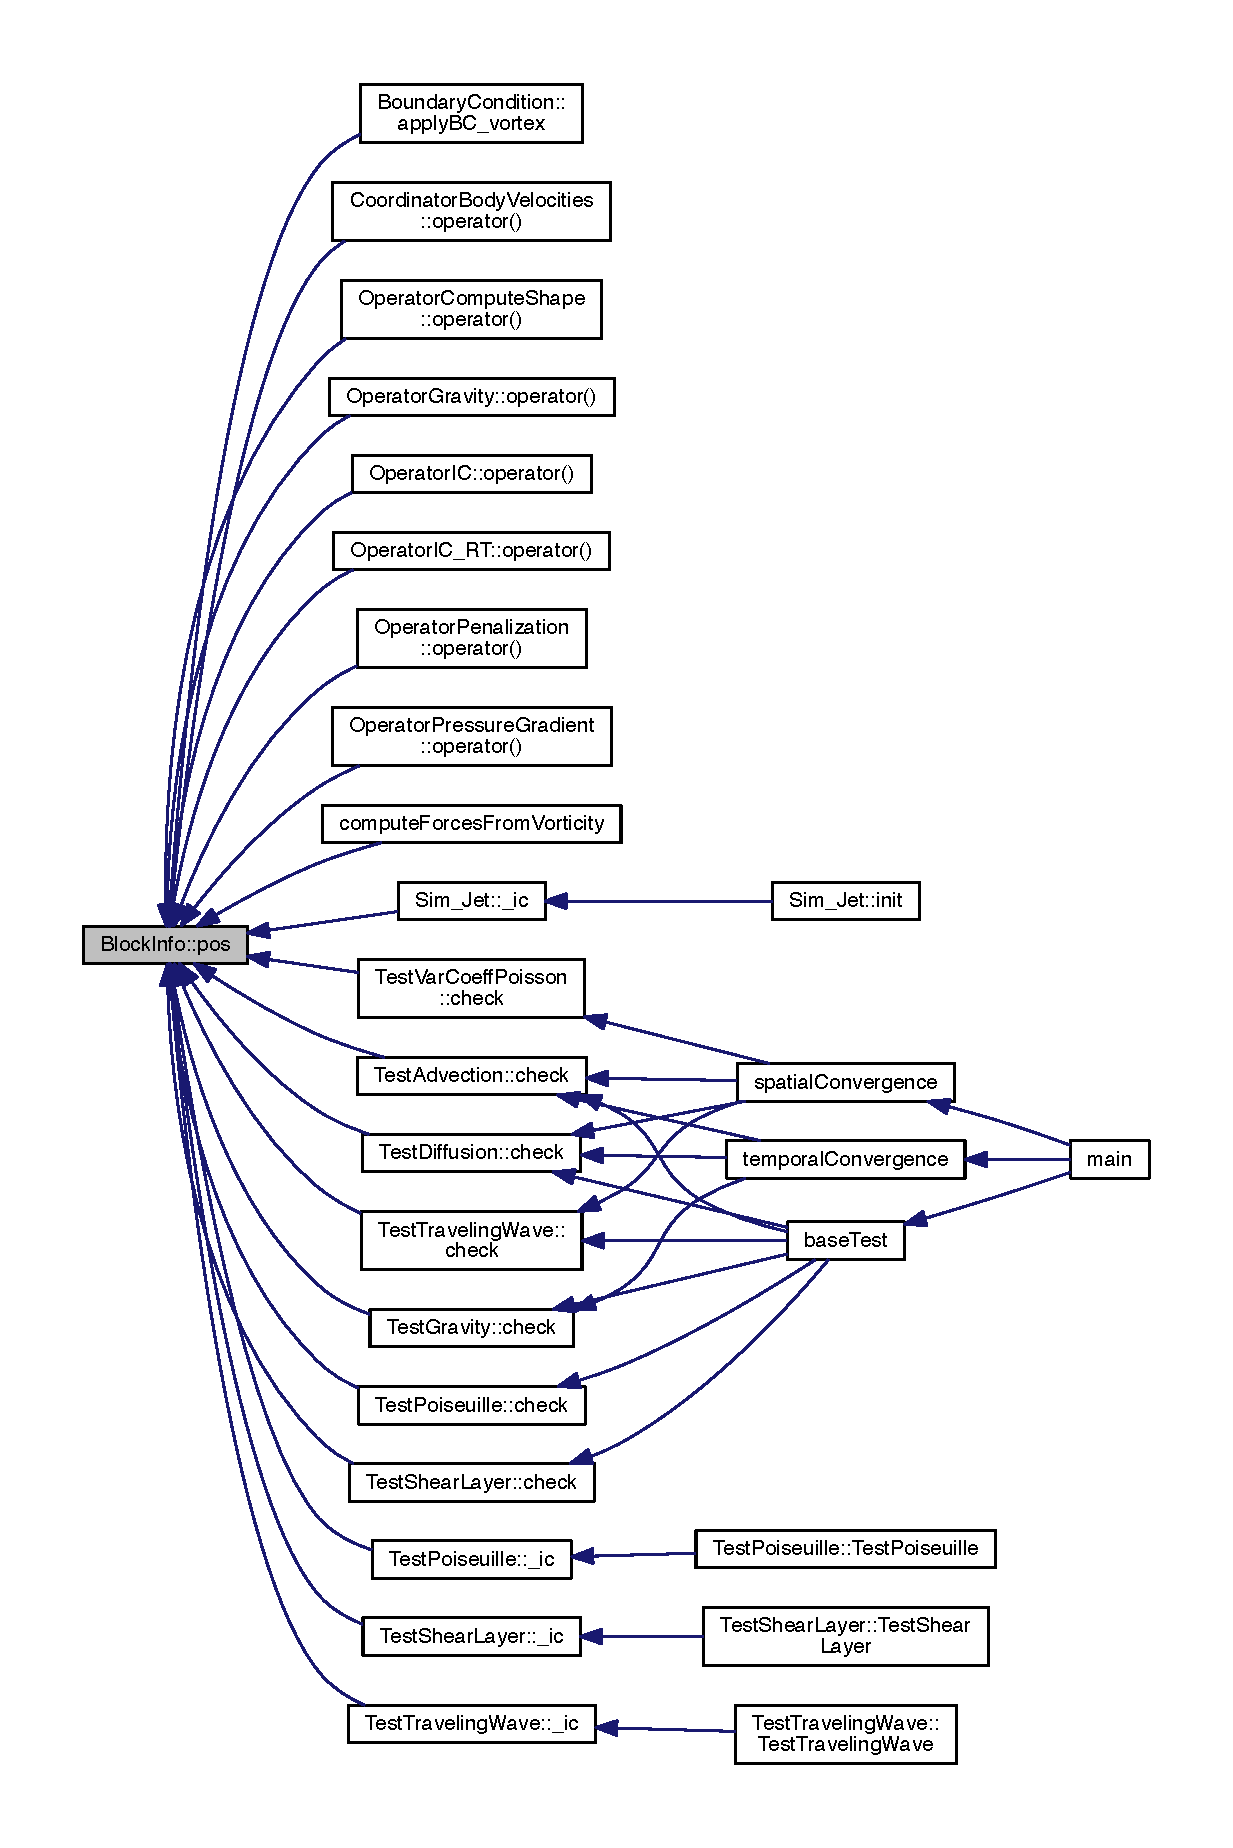
\includegraphics[width=350pt]{d4/ded/struct_block_info_abcc226bdb973d09286902ae23f3962fd_icgraph}
\end{center}
\end{figure}


\hypertarget{struct_block_info_a803920cf6f3185de720fe789fa59f6cb}{}\index{Block\+Info@{Block\+Info}!pos@{pos}}
\index{pos@{pos}!Block\+Info@{Block\+Info}}
\subsubsection[{pos}]{\setlength{\rightskip}{0pt plus 5cm}template$<$typename T $>$ void Block\+Info\+::pos (
\begin{DoxyParamCaption}
\item[{T}]{p\mbox{[}3\mbox{]}, }
\item[{int}]{ix, }
\item[{int}]{iy, }
\item[{int}]{iz}
\end{DoxyParamCaption}
) const\hspace{0.3cm}{\ttfamily [inline]}}\label{struct_block_info_a803920cf6f3185de720fe789fa59f6cb}


\subsection{Member Data Documentation}
\hypertarget{struct_block_info_aff4a50657c14cc550c9e0e3aaaed1a15}{}\index{Block\+Info@{Block\+Info}!block\+I\+D@{block\+I\+D}}
\index{block\+I\+D@{block\+I\+D}!Block\+Info@{Block\+Info}}
\subsubsection[{block\+I\+D}]{\setlength{\rightskip}{0pt plus 5cm}long long Block\+Info\+::block\+I\+D}\label{struct_block_info_aff4a50657c14cc550c9e0e3aaaed1a15}
\hypertarget{struct_block_info_abb250cd39311bd0a840588ff2a6196ad}{}\index{Block\+Info@{Block\+Info}!h@{h}}
\index{h@{h}!Block\+Info@{Block\+Info}}
\subsubsection[{h}]{\setlength{\rightskip}{0pt plus 5cm}double Block\+Info\+::h}\label{struct_block_info_abb250cd39311bd0a840588ff2a6196ad}
\hypertarget{struct_block_info_a83bd46701539e64d666206d6501ee3ea}{}\index{Block\+Info@{Block\+Info}!h\+\_\+gridpoint@{h\+\_\+gridpoint}}
\index{h\+\_\+gridpoint@{h\+\_\+gridpoint}!Block\+Info@{Block\+Info}}
\subsubsection[{h\+\_\+gridpoint}]{\setlength{\rightskip}{0pt plus 5cm}double Block\+Info\+::h\+\_\+gridpoint}\label{struct_block_info_a83bd46701539e64d666206d6501ee3ea}
\hypertarget{struct_block_info_ad32832aaa2dee35464a74abfae741572}{}\index{Block\+Info@{Block\+Info}!index@{index}}
\index{index@{index}!Block\+Info@{Block\+Info}}
\subsubsection[{index}]{\setlength{\rightskip}{0pt plus 5cm}int Block\+Info\+::index\mbox{[}3\mbox{]}}\label{struct_block_info_ad32832aaa2dee35464a74abfae741572}
\hypertarget{struct_block_info_a8d2d03097cfbffc58d3cc2dee371e4b2}{}\index{Block\+Info@{Block\+Info}!origin@{origin}}
\index{origin@{origin}!Block\+Info@{Block\+Info}}
\subsubsection[{origin}]{\setlength{\rightskip}{0pt plus 5cm}double Block\+Info\+::origin\mbox{[}3\mbox{]}}\label{struct_block_info_a8d2d03097cfbffc58d3cc2dee371e4b2}
\hypertarget{struct_block_info_af3655416c17becfb24a9f475a7b97d23}{}\index{Block\+Info@{Block\+Info}!ptr\+Block@{ptr\+Block}}
\index{ptr\+Block@{ptr\+Block}!Block\+Info@{Block\+Info}}
\subsubsection[{ptr\+Block}]{\setlength{\rightskip}{0pt plus 5cm}void$\ast$ Block\+Info\+::ptr\+Block}\label{struct_block_info_af3655416c17becfb24a9f475a7b97d23}


The documentation for this struct was generated from the following file\+:\begin{DoxyCompactItemize}
\item 
/\+Users/cconti/\+Desktop/\+Mounts/\+Brutus\+Home/\+Cubism\+U\+P\+\_\+2\+D/\+Cubism/\hyperlink{_block_info_8h}{Block\+Info.\+h}\end{DoxyCompactItemize}

\hypertarget{class_block_lab}{}\section{Block\+Lab$<$ T\+Block, allocator, Element\+Type\+T $>$ Class Template Reference}
\label{class_block_lab}\index{Block\+Lab$<$ T\+Block, allocator, Element\+Type\+T $>$@{Block\+Lab$<$ T\+Block, allocator, Element\+Type\+T $>$}}


{\ttfamily \#include $<$Block\+Lab.\+h$>$}



Collaboration diagram for Block\+Lab$<$ T\+Block, allocator, Element\+Type\+T $>$\+:\nopagebreak
\begin{figure}[H]
\begin{center}
\leavevmode
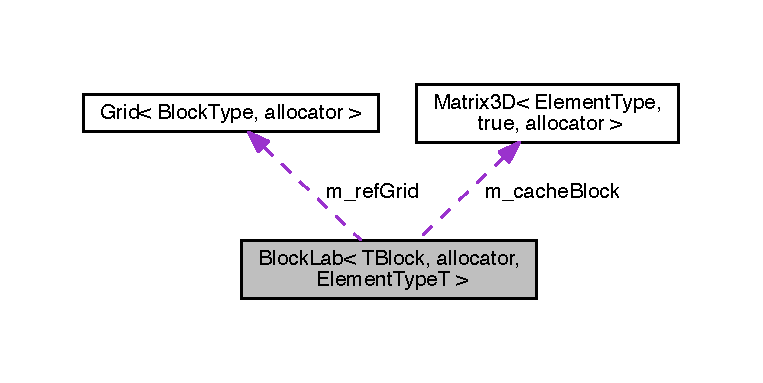
\includegraphics[width=350pt]{da/daa/class_block_lab__coll__graph}
\end{center}
\end{figure}
\subsection*{Public Types}
\begin{DoxyCompactItemize}
\item 
typedef Element\+Type\+T \hyperlink{class_block_lab_accdcd2d5e815a8497e5ef9ae884da6b6}{Element\+Type}
\end{DoxyCompactItemize}
\subsection*{Public Member Functions}
\begin{DoxyCompactItemize}
\item 
\hyperlink{class_block_lab_a0cb8aec5f42c4b1860be8aa218660087}{Block\+Lab} ()
\item 
virtual bool \hyperlink{class_block_lab_aaf6e3ab940c5c3cf7463bad112527f98}{is\+\_\+xperiodic} ()
\item 
virtual bool \hyperlink{class_block_lab_a5455e54c8e874ee9da6159ea0d1651ed}{is\+\_\+yperiodic} ()
\item 
virtual bool \hyperlink{class_block_lab_a0fd3a720fb3f2f76845ff4323e89bb91}{is\+\_\+zperiodic} ()
\item 
\hyperlink{class_block_lab_a083218471f59c32fccc335759734667d}{$\sim$\+Block\+Lab} ()
\item 
{\footnotesize template$<$int dim$>$ }\\int \hyperlink{class_block_lab_aa45e40066bececd40de75c238c346e79}{get\+Actual\+Size} () const 
\item 
\hyperlink{class_block_lab_accdcd2d5e815a8497e5ef9ae884da6b6}{Element\+Type} $\ast$ \hyperlink{class_block_lab_a4dd07a50f8766b29717b9326e67a9fcd}{get\+Buffer} () const 
\item 
void \hyperlink{class_block_lab_ad529f8c851da336419ad63c25ba76429}{prepare} (\hyperlink{class_grid}{Grid}$<$ \hyperlink{class_block_lab_a745b3c9ac17f6743d11a7085196981a0}{Block\+Type}, allocator $>$ \&grid, int start\+X, int end\+X, int start\+Y, int end\+Y, int start\+Z, int end\+Z, const bool \hyperlink{class_block_lab_ade306bb6935a0ead765444534c2e05db}{istensorial})
\item 
void \hyperlink{class_block_lab_ac6236e1c94d13fa1025c8253b9855a04}{prepare} (\hyperlink{class_grid}{Grid}$<$ \hyperlink{class_block_lab_a745b3c9ac17f6743d11a7085196981a0}{Block\+Type}, allocator $>$ \&grid, const int stencil\+\_\+start\mbox{[}3\mbox{]}, const int stencil\+\_\+end\mbox{[}3\mbox{]}, const bool \hyperlink{class_block_lab_ade306bb6935a0ead765444534c2e05db}{istensorial})
\item 
void \hyperlink{class_block_lab_aefd27fed8fbb1d3d60fe1457ae90f248}{load} (const \hyperlink{struct_block_info}{Block\+Info} \&info, const \hyperlink{_h_d_f5_dumper_8h_a445a5f0e2a34c9d97d69a3c2d1957907}{Real} t=0, const bool applybc=true)
\item 
\hyperlink{class_block_lab_accdcd2d5e815a8497e5ef9ae884da6b6}{Element\+Type} \& \hyperlink{class_block_lab_abd79a09ab5b54cf04bfe25c125ea1edf}{operator()} (int ix, int iy=0, int iz=0)
\item 
const \hyperlink{class_block_lab_accdcd2d5e815a8497e5ef9ae884da6b6}{Element\+Type} \& \hyperlink{class_block_lab_a3e06d4124f7d69923b4ee6345c105cfc}{read} (int ix, int iy=0, int iz=0) const 
\end{DoxyCompactItemize}
\subsection*{Protected Types}
\begin{DoxyCompactItemize}
\item 
enum \hyperlink{class_block_lab_ad3a1e6e1a1002fb812d6853c8ac1ec9e}{e\+Block\+Lab\+\_\+\+State} \{ \hyperlink{class_block_lab_ad3a1e6e1a1002fb812d6853c8ac1ec9ea6c1a64be2e953c6093dab00aab32fe00}{e\+M\+R\+A\+G\+Block\+Lab\+\_\+\+Prepared}, 
\hyperlink{class_block_lab_ad3a1e6e1a1002fb812d6853c8ac1ec9eadaaa507dbe601b991a383e6a0701a09c}{e\+M\+R\+A\+G\+Block\+Lab\+\_\+\+Loaded}, 
\hyperlink{class_block_lab_ad3a1e6e1a1002fb812d6853c8ac1ec9ead9471f6585bd7cf7ddc9edad96e67362}{e\+M\+R\+A\+G\+Block\+Lab\+\_\+\+Uninitialized}
 \}
\item 
typedef T\+Block \hyperlink{class_block_lab_a745b3c9ac17f6743d11a7085196981a0}{Block\+Type}
\item 
typedef Block\+Type\+::\+Element\+Type \hyperlink{class_block_lab_ad547d74881a0d226a849e2051af6b26b}{Element\+Type\+Block}
\end{DoxyCompactItemize}
\subsection*{Protected Member Functions}
\begin{DoxyCompactItemize}
\item 
virtual void \hyperlink{class_block_lab_a669ac139b57be4967e5f43bc649a8520}{\+\_\+apply\+\_\+bc} (const \hyperlink{struct_block_info}{Block\+Info} \&info, const \hyperlink{_h_d_f5_dumper_8h_a445a5f0e2a34c9d97d69a3c2d1957907}{Real} t=0)
\item 
{\footnotesize template$<$typename T $>$ }\\void \hyperlink{class_block_lab_ab23c907953858c8b393a9910ecf5b1cf}{\+\_\+release} (T $\ast$\&t)
\end{DoxyCompactItemize}
\subsection*{Protected Attributes}
\begin{DoxyCompactItemize}
\item 
\hyperlink{class_block_lab_ad3a1e6e1a1002fb812d6853c8ac1ec9e}{e\+Block\+Lab\+\_\+\+State} \hyperlink{class_block_lab_a0e11603d73ab4923e1d9033edccdb572}{m\+\_\+state}
\item 
\hyperlink{class_matrix3_d}{Matrix3\+D}$<$ \hyperlink{class_block_lab_accdcd2d5e815a8497e5ef9ae884da6b6}{Element\+Type}, true, allocator $>$ $\ast$ \hyperlink{class_block_lab_aa6a4c4e00a9bb5ca5780d820b146485b}{m\+\_\+cache\+Block}
\item 
int \hyperlink{class_block_lab_a8ac6690f98ba84346a74b5b95c3afb2b}{m\+\_\+stencil\+Start} \mbox{[}3\mbox{]}
\item 
int \hyperlink{class_block_lab_a46fee08b49b11be489c71f726e258cc9}{m\+\_\+stencil\+End} \mbox{[}3\mbox{]}
\item 
int \hyperlink{class_block_lab_abcd7367c6f45124d3202c8da5043ac93}{N\+X}
\item 
int \hyperlink{class_block_lab_aaa1e748664ebb6b4fc7c47cf30a445db}{N\+Y}
\item 
int \hyperlink{class_block_lab_acdd7f4e2489d31da6a2a76099807a7c5}{N\+Z}
\item 
bool \hyperlink{class_block_lab_ade306bb6935a0ead765444534c2e05db}{istensorial}
\item 
const \hyperlink{class_grid}{Grid}$<$ \hyperlink{class_block_lab_a745b3c9ac17f6743d11a7085196981a0}{Block\+Type}, allocator $>$ $\ast$ \hyperlink{class_block_lab_acccfe85f166f20526118fce09b28fb04}{m\+\_\+ref\+Grid}
\end{DoxyCompactItemize}


\subsection{Detailed Description}
\subsubsection*{template$<$typename T\+Block, template$<$ typename X $>$ class allocator = std\+::allocator, typename Element\+Type\+T = typename T\+Block\+::\+Element\+Type$>$class Block\+Lab$<$ T\+Block, allocator, Element\+Type\+T $>$}

Working copy of Block + Ghosts. Data of original block is copied (!) here. So when changing something in the lab we are not changing the original data. Requirements\+:
\begin{DoxyItemize}
\item Concepts\+::\+Block\+Lab\+Element\+Type$<$\+Element\+Type\+T$>$
\item Concepts\+::\+Castable$<$typename Block\+Type\+::\+Element\+Type, Element\+Type\+T$>$ 
\end{DoxyItemize}

\subsection{Member Typedef Documentation}
\hypertarget{class_block_lab_a745b3c9ac17f6743d11a7085196981a0}{}\index{Block\+Lab@{Block\+Lab}!Block\+Type@{Block\+Type}}
\index{Block\+Type@{Block\+Type}!Block\+Lab@{Block\+Lab}}
\subsubsection[{Block\+Type}]{\setlength{\rightskip}{0pt plus 5cm}template$<$typename T\+Block, template$<$ typename X $>$ class allocator = std\+::allocator, typename Element\+Type\+T = typename T\+Block\+::\+Element\+Type$>$ typedef T\+Block {\bf Block\+Lab}$<$ T\+Block, allocator, Element\+Type\+T $>$\+::{\bf Block\+Type}\hspace{0.3cm}{\ttfamily [protected]}}\label{class_block_lab_a745b3c9ac17f6743d11a7085196981a0}
\hypertarget{class_block_lab_accdcd2d5e815a8497e5ef9ae884da6b6}{}\index{Block\+Lab@{Block\+Lab}!Element\+Type@{Element\+Type}}
\index{Element\+Type@{Element\+Type}!Block\+Lab@{Block\+Lab}}
\subsubsection[{Element\+Type}]{\setlength{\rightskip}{0pt plus 5cm}template$<$typename T\+Block, template$<$ typename X $>$ class allocator = std\+::allocator, typename Element\+Type\+T = typename T\+Block\+::\+Element\+Type$>$ typedef Element\+Type\+T {\bf Block\+Lab}$<$ T\+Block, allocator, Element\+Type\+T $>$\+::{\bf Element\+Type}}\label{class_block_lab_accdcd2d5e815a8497e5ef9ae884da6b6}
\hypertarget{class_block_lab_ad547d74881a0d226a849e2051af6b26b}{}\index{Block\+Lab@{Block\+Lab}!Element\+Type\+Block@{Element\+Type\+Block}}
\index{Element\+Type\+Block@{Element\+Type\+Block}!Block\+Lab@{Block\+Lab}}
\subsubsection[{Element\+Type\+Block}]{\setlength{\rightskip}{0pt plus 5cm}template$<$typename T\+Block, template$<$ typename X $>$ class allocator = std\+::allocator, typename Element\+Type\+T = typename T\+Block\+::\+Element\+Type$>$ typedef Block\+Type\+::\+Element\+Type {\bf Block\+Lab}$<$ T\+Block, allocator, Element\+Type\+T $>$\+::{\bf Element\+Type\+Block}\hspace{0.3cm}{\ttfamily [protected]}}\label{class_block_lab_ad547d74881a0d226a849e2051af6b26b}


\subsection{Member Enumeration Documentation}
\hypertarget{class_block_lab_ad3a1e6e1a1002fb812d6853c8ac1ec9e}{}\index{Block\+Lab@{Block\+Lab}!e\+Block\+Lab\+\_\+\+State@{e\+Block\+Lab\+\_\+\+State}}
\index{e\+Block\+Lab\+\_\+\+State@{e\+Block\+Lab\+\_\+\+State}!Block\+Lab@{Block\+Lab}}
\subsubsection[{e\+Block\+Lab\+\_\+\+State}]{\setlength{\rightskip}{0pt plus 5cm}template$<$typename T\+Block, template$<$ typename X $>$ class allocator = std\+::allocator, typename Element\+Type\+T = typename T\+Block\+::\+Element\+Type$>$ enum {\bf Block\+Lab\+::e\+Block\+Lab\+\_\+\+State}\hspace{0.3cm}{\ttfamily [protected]}}\label{class_block_lab_ad3a1e6e1a1002fb812d6853c8ac1ec9e}
\begin{Desc}
\item[Enumerator]\par
\begin{description}
\index{e\+M\+R\+A\+G\+Block\+Lab\+\_\+\+Prepared@{e\+M\+R\+A\+G\+Block\+Lab\+\_\+\+Prepared}!Block\+Lab@{Block\+Lab}}\index{Block\+Lab@{Block\+Lab}!e\+M\+R\+A\+G\+Block\+Lab\+\_\+\+Prepared@{e\+M\+R\+A\+G\+Block\+Lab\+\_\+\+Prepared}}\item[{\em 
\hypertarget{class_block_lab_ad3a1e6e1a1002fb812d6853c8ac1ec9ea6c1a64be2e953c6093dab00aab32fe00}{}e\+M\+R\+A\+G\+Block\+Lab\+\_\+\+Prepared\label{class_block_lab_ad3a1e6e1a1002fb812d6853c8ac1ec9ea6c1a64be2e953c6093dab00aab32fe00}
}]\index{e\+M\+R\+A\+G\+Block\+Lab\+\_\+\+Loaded@{e\+M\+R\+A\+G\+Block\+Lab\+\_\+\+Loaded}!Block\+Lab@{Block\+Lab}}\index{Block\+Lab@{Block\+Lab}!e\+M\+R\+A\+G\+Block\+Lab\+\_\+\+Loaded@{e\+M\+R\+A\+G\+Block\+Lab\+\_\+\+Loaded}}\item[{\em 
\hypertarget{class_block_lab_ad3a1e6e1a1002fb812d6853c8ac1ec9eadaaa507dbe601b991a383e6a0701a09c}{}e\+M\+R\+A\+G\+Block\+Lab\+\_\+\+Loaded\label{class_block_lab_ad3a1e6e1a1002fb812d6853c8ac1ec9eadaaa507dbe601b991a383e6a0701a09c}
}]\index{e\+M\+R\+A\+G\+Block\+Lab\+\_\+\+Uninitialized@{e\+M\+R\+A\+G\+Block\+Lab\+\_\+\+Uninitialized}!Block\+Lab@{Block\+Lab}}\index{Block\+Lab@{Block\+Lab}!e\+M\+R\+A\+G\+Block\+Lab\+\_\+\+Uninitialized@{e\+M\+R\+A\+G\+Block\+Lab\+\_\+\+Uninitialized}}\item[{\em 
\hypertarget{class_block_lab_ad3a1e6e1a1002fb812d6853c8ac1ec9ead9471f6585bd7cf7ddc9edad96e67362}{}e\+M\+R\+A\+G\+Block\+Lab\+\_\+\+Uninitialized\label{class_block_lab_ad3a1e6e1a1002fb812d6853c8ac1ec9ead9471f6585bd7cf7ddc9edad96e67362}
}]\end{description}
\end{Desc}


\subsection{Constructor \& Destructor Documentation}
\hypertarget{class_block_lab_a0cb8aec5f42c4b1860be8aa218660087}{}\index{Block\+Lab@{Block\+Lab}!Block\+Lab@{Block\+Lab}}
\index{Block\+Lab@{Block\+Lab}!Block\+Lab@{Block\+Lab}}
\subsubsection[{Block\+Lab}]{\setlength{\rightskip}{0pt plus 5cm}template$<$typename T\+Block, template$<$ typename X $>$ class allocator = std\+::allocator, typename Element\+Type\+T = typename T\+Block\+::\+Element\+Type$>$ {\bf Block\+Lab}$<$ T\+Block, allocator, Element\+Type\+T $>$\+::{\bf Block\+Lab} (
\begin{DoxyParamCaption}
{}
\end{DoxyParamCaption}
)\hspace{0.3cm}{\ttfamily [inline]}}\label{class_block_lab_a0cb8aec5f42c4b1860be8aa218660087}
\hypertarget{class_block_lab_a083218471f59c32fccc335759734667d}{}\index{Block\+Lab@{Block\+Lab}!````~Block\+Lab@{$\sim$\+Block\+Lab}}
\index{````~Block\+Lab@{$\sim$\+Block\+Lab}!Block\+Lab@{Block\+Lab}}
\subsubsection[{$\sim$\+Block\+Lab}]{\setlength{\rightskip}{0pt plus 5cm}template$<$typename T\+Block, template$<$ typename X $>$ class allocator = std\+::allocator, typename Element\+Type\+T = typename T\+Block\+::\+Element\+Type$>$ {\bf Block\+Lab}$<$ T\+Block, allocator, Element\+Type\+T $>$\+::$\sim${\bf Block\+Lab} (
\begin{DoxyParamCaption}
{}
\end{DoxyParamCaption}
)\hspace{0.3cm}{\ttfamily [inline]}}\label{class_block_lab_a083218471f59c32fccc335759734667d}


\subsection{Member Function Documentation}
\hypertarget{class_block_lab_a669ac139b57be4967e5f43bc649a8520}{}\index{Block\+Lab@{Block\+Lab}!\+\_\+apply\+\_\+bc@{\+\_\+apply\+\_\+bc}}
\index{\+\_\+apply\+\_\+bc@{\+\_\+apply\+\_\+bc}!Block\+Lab@{Block\+Lab}}
\subsubsection[{\+\_\+apply\+\_\+bc}]{\setlength{\rightskip}{0pt plus 5cm}template$<$typename T\+Block, template$<$ typename X $>$ class allocator = std\+::allocator, typename Element\+Type\+T = typename T\+Block\+::\+Element\+Type$>$ virtual void {\bf Block\+Lab}$<$ T\+Block, allocator, Element\+Type\+T $>$\+::\+\_\+apply\+\_\+bc (
\begin{DoxyParamCaption}
\item[{const {\bf Block\+Info} \&}]{info, }
\item[{const {\bf Real}}]{t = {\ttfamily 0}}
\end{DoxyParamCaption}
)\hspace{0.3cm}{\ttfamily [inline]}, {\ttfamily [protected]}, {\ttfamily [virtual]}}\label{class_block_lab_a669ac139b57be4967e5f43bc649a8520}


Reimplemented in \hyperlink{class_block_lab_box_adfd9b3d46062be59f03d0c1df79db81d}{Block\+Lab\+Box$<$ Block\+Type, allocator $>$}, \hyperlink{class_block_lab_neumann_a65cd80126a426fa2aa098910fd189793}{Block\+Lab\+Neumann$<$ Block\+Type, allocator $>$}, and \hyperlink{class_block_lab_dirichlet_ae05580142a8ddb65c42fd92063355609}{Block\+Lab\+Dirichlet$<$ Block\+Type, allocator $>$}.



Here is the caller graph for this function\+:\nopagebreak
\begin{figure}[H]
\begin{center}
\leavevmode
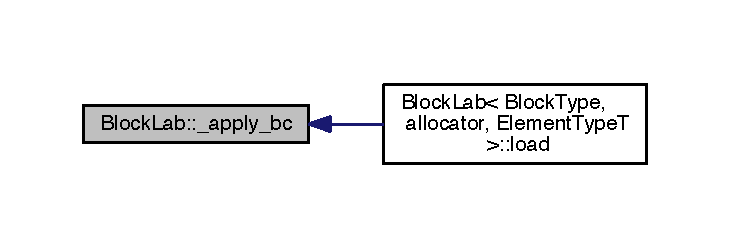
\includegraphics[width=350pt]{d7/d95/class_block_lab_a669ac139b57be4967e5f43bc649a8520_icgraph}
\end{center}
\end{figure}


\hypertarget{class_block_lab_ab23c907953858c8b393a9910ecf5b1cf}{}\index{Block\+Lab@{Block\+Lab}!\+\_\+release@{\+\_\+release}}
\index{\+\_\+release@{\+\_\+release}!Block\+Lab@{Block\+Lab}}
\subsubsection[{\+\_\+release}]{\setlength{\rightskip}{0pt plus 5cm}template$<$typename T\+Block, template$<$ typename X $>$ class allocator = std\+::allocator, typename Element\+Type\+T = typename T\+Block\+::\+Element\+Type$>$ template$<$typename T $>$ void {\bf Block\+Lab}$<$ T\+Block, allocator, Element\+Type\+T $>$\+::\+\_\+release (
\begin{DoxyParamCaption}
\item[{T $\ast$\&}]{t}
\end{DoxyParamCaption}
)\hspace{0.3cm}{\ttfamily [inline]}, {\ttfamily [protected]}}\label{class_block_lab_ab23c907953858c8b393a9910ecf5b1cf}


Here is the caller graph for this function\+:\nopagebreak
\begin{figure}[H]
\begin{center}
\leavevmode
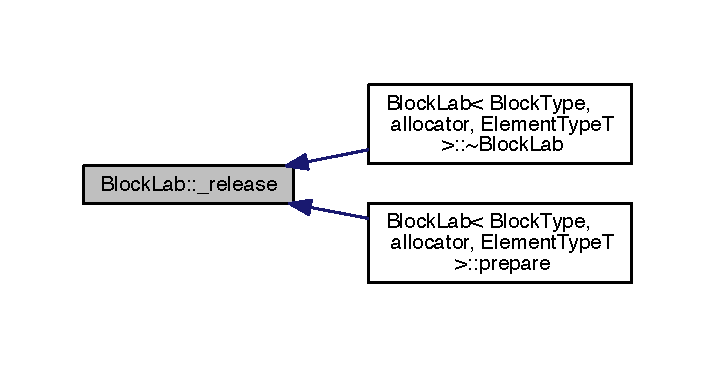
\includegraphics[width=343pt]{d7/d95/class_block_lab_ab23c907953858c8b393a9910ecf5b1cf_icgraph}
\end{center}
\end{figure}


\hypertarget{class_block_lab_aa45e40066bececd40de75c238c346e79}{}\index{Block\+Lab@{Block\+Lab}!get\+Actual\+Size@{get\+Actual\+Size}}
\index{get\+Actual\+Size@{get\+Actual\+Size}!Block\+Lab@{Block\+Lab}}
\subsubsection[{get\+Actual\+Size}]{\setlength{\rightskip}{0pt plus 5cm}template$<$typename T\+Block, template$<$ typename X $>$ class allocator = std\+::allocator, typename Element\+Type\+T = typename T\+Block\+::\+Element\+Type$>$ template$<$int dim$>$ int {\bf Block\+Lab}$<$ T\+Block, allocator, Element\+Type\+T $>$\+::get\+Actual\+Size (
\begin{DoxyParamCaption}
{}
\end{DoxyParamCaption}
) const\hspace{0.3cm}{\ttfamily [inline]}}\label{class_block_lab_aa45e40066bececd40de75c238c346e79}
\hypertarget{class_block_lab_a4dd07a50f8766b29717b9326e67a9fcd}{}\index{Block\+Lab@{Block\+Lab}!get\+Buffer@{get\+Buffer}}
\index{get\+Buffer@{get\+Buffer}!Block\+Lab@{Block\+Lab}}
\subsubsection[{get\+Buffer}]{\setlength{\rightskip}{0pt plus 5cm}template$<$typename T\+Block, template$<$ typename X $>$ class allocator = std\+::allocator, typename Element\+Type\+T = typename T\+Block\+::\+Element\+Type$>$ {\bf Element\+Type}$\ast$ {\bf Block\+Lab}$<$ T\+Block, allocator, Element\+Type\+T $>$\+::get\+Buffer (
\begin{DoxyParamCaption}
{}
\end{DoxyParamCaption}
) const\hspace{0.3cm}{\ttfamily [inline]}}\label{class_block_lab_a4dd07a50f8766b29717b9326e67a9fcd}
\hypertarget{class_block_lab_aaf6e3ab940c5c3cf7463bad112527f98}{}\index{Block\+Lab@{Block\+Lab}!is\+\_\+xperiodic@{is\+\_\+xperiodic}}
\index{is\+\_\+xperiodic@{is\+\_\+xperiodic}!Block\+Lab@{Block\+Lab}}
\subsubsection[{is\+\_\+xperiodic}]{\setlength{\rightskip}{0pt plus 5cm}template$<$typename T\+Block, template$<$ typename X $>$ class allocator = std\+::allocator, typename Element\+Type\+T = typename T\+Block\+::\+Element\+Type$>$ virtual bool {\bf Block\+Lab}$<$ T\+Block, allocator, Element\+Type\+T $>$\+::is\+\_\+xperiodic (
\begin{DoxyParamCaption}
{}
\end{DoxyParamCaption}
)\hspace{0.3cm}{\ttfamily [inline]}, {\ttfamily [virtual]}}\label{class_block_lab_aaf6e3ab940c5c3cf7463bad112527f98}


Here is the caller graph for this function\+:\nopagebreak
\begin{figure}[H]
\begin{center}
\leavevmode
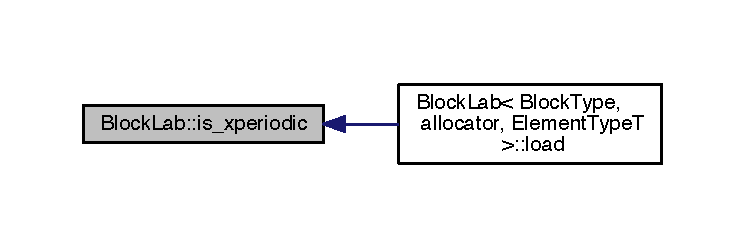
\includegraphics[width=350pt]{d7/d95/class_block_lab_aaf6e3ab940c5c3cf7463bad112527f98_icgraph}
\end{center}
\end{figure}


\hypertarget{class_block_lab_a5455e54c8e874ee9da6159ea0d1651ed}{}\index{Block\+Lab@{Block\+Lab}!is\+\_\+yperiodic@{is\+\_\+yperiodic}}
\index{is\+\_\+yperiodic@{is\+\_\+yperiodic}!Block\+Lab@{Block\+Lab}}
\subsubsection[{is\+\_\+yperiodic}]{\setlength{\rightskip}{0pt plus 5cm}template$<$typename T\+Block, template$<$ typename X $>$ class allocator = std\+::allocator, typename Element\+Type\+T = typename T\+Block\+::\+Element\+Type$>$ virtual bool {\bf Block\+Lab}$<$ T\+Block, allocator, Element\+Type\+T $>$\+::is\+\_\+yperiodic (
\begin{DoxyParamCaption}
{}
\end{DoxyParamCaption}
)\hspace{0.3cm}{\ttfamily [inline]}, {\ttfamily [virtual]}}\label{class_block_lab_a5455e54c8e874ee9da6159ea0d1651ed}


Here is the caller graph for this function\+:\nopagebreak
\begin{figure}[H]
\begin{center}
\leavevmode
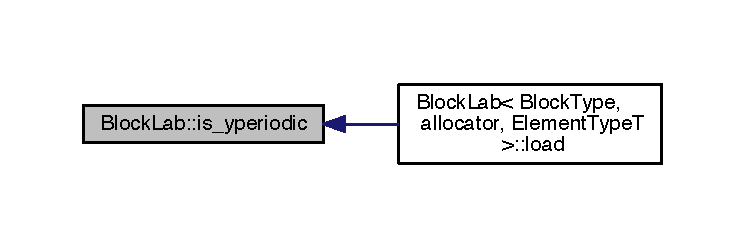
\includegraphics[width=350pt]{d7/d95/class_block_lab_a5455e54c8e874ee9da6159ea0d1651ed_icgraph}
\end{center}
\end{figure}


\hypertarget{class_block_lab_a0fd3a720fb3f2f76845ff4323e89bb91}{}\index{Block\+Lab@{Block\+Lab}!is\+\_\+zperiodic@{is\+\_\+zperiodic}}
\index{is\+\_\+zperiodic@{is\+\_\+zperiodic}!Block\+Lab@{Block\+Lab}}
\subsubsection[{is\+\_\+zperiodic}]{\setlength{\rightskip}{0pt plus 5cm}template$<$typename T\+Block, template$<$ typename X $>$ class allocator = std\+::allocator, typename Element\+Type\+T = typename T\+Block\+::\+Element\+Type$>$ virtual bool {\bf Block\+Lab}$<$ T\+Block, allocator, Element\+Type\+T $>$\+::is\+\_\+zperiodic (
\begin{DoxyParamCaption}
{}
\end{DoxyParamCaption}
)\hspace{0.3cm}{\ttfamily [inline]}, {\ttfamily [virtual]}}\label{class_block_lab_a0fd3a720fb3f2f76845ff4323e89bb91}


Here is the caller graph for this function\+:\nopagebreak
\begin{figure}[H]
\begin{center}
\leavevmode
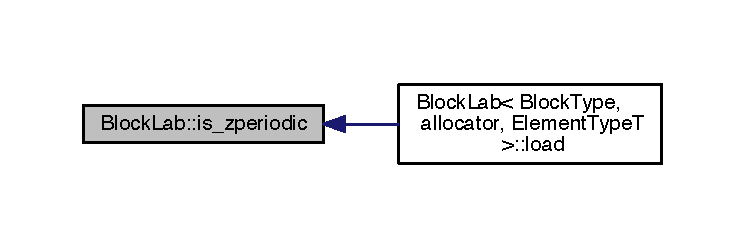
\includegraphics[width=350pt]{d7/d95/class_block_lab_a0fd3a720fb3f2f76845ff4323e89bb91_icgraph}
\end{center}
\end{figure}


\hypertarget{class_block_lab_aefd27fed8fbb1d3d60fe1457ae90f248}{}\index{Block\+Lab@{Block\+Lab}!load@{load}}
\index{load@{load}!Block\+Lab@{Block\+Lab}}
\subsubsection[{load}]{\setlength{\rightskip}{0pt plus 5cm}template$<$typename T\+Block, template$<$ typename X $>$ class allocator = std\+::allocator, typename Element\+Type\+T = typename T\+Block\+::\+Element\+Type$>$ void {\bf Block\+Lab}$<$ T\+Block, allocator, Element\+Type\+T $>$\+::load (
\begin{DoxyParamCaption}
\item[{const {\bf Block\+Info} \&}]{info, }
\item[{const {\bf Real}}]{t = {\ttfamily 0}, }
\item[{const bool}]{applybc = {\ttfamily true}}
\end{DoxyParamCaption}
)\hspace{0.3cm}{\ttfamily [inline]}}\label{class_block_lab_aefd27fed8fbb1d3d60fe1457ae90f248}
Load a block (incl. ghosts for it). This is not called internally but by the Block\+Processing-\/class. Hence a new version of \hyperlink{class_block_lab}{Block\+Lab}, can just overwrite it and through template-\/passing to Block\+Processing, the right version will be called. 
\begin{DoxyParams}{Parameters}
{\em info} & Reference to info of block to be loaded. \\
\hline
\end{DoxyParams}


Here is the caller graph for this function\+:\nopagebreak
\begin{figure}[H]
\begin{center}
\leavevmode
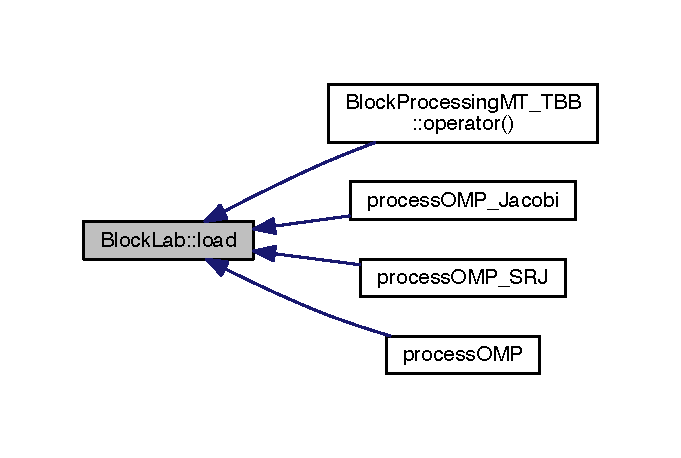
\includegraphics[width=327pt]{d7/d95/class_block_lab_aefd27fed8fbb1d3d60fe1457ae90f248_icgraph}
\end{center}
\end{figure}


\hypertarget{class_block_lab_abd79a09ab5b54cf04bfe25c125ea1edf}{}\index{Block\+Lab@{Block\+Lab}!operator()@{operator()}}
\index{operator()@{operator()}!Block\+Lab@{Block\+Lab}}
\subsubsection[{operator()}]{\setlength{\rightskip}{0pt plus 5cm}template$<$typename T\+Block, template$<$ typename X $>$ class allocator = std\+::allocator, typename Element\+Type\+T = typename T\+Block\+::\+Element\+Type$>$ {\bf Element\+Type}\& {\bf Block\+Lab}$<$ T\+Block, allocator, Element\+Type\+T $>$\+::operator() (
\begin{DoxyParamCaption}
\item[{int}]{ix, }
\item[{int}]{iy = {\ttfamily 0}, }
\item[{int}]{iz = {\ttfamily 0}}
\end{DoxyParamCaption}
)\hspace{0.3cm}{\ttfamily [inline]}}\label{class_block_lab_abd79a09ab5b54cf04bfe25c125ea1edf}
Get a single element from the block. stencil\+\_\+start and stencil\+\_\+end refer to the values passed in \hyperlink{class_block_lab_ad529f8c851da336419ad63c25ba76429}{Block\+Lab\+::prepare()}.


\begin{DoxyParams}{Parameters}
{\em ix} & Index in x-\/direction (stencil\+\_\+start\mbox{[}0\mbox{]} $<$= ix $<$ Block\+Type\+::size\+X + stencil\+\_\+end\mbox{[}0\mbox{]} -\/ 1). \\
\hline
{\em iy} & Index in y-\/direction (stencil\+\_\+start\mbox{[}1\mbox{]} $<$= iy $<$ Block\+Type\+::size\+Y + stencil\+\_\+end\mbox{[}1\mbox{]} -\/ 1). \\
\hline
{\em iz} & Index in z-\/direction (stencil\+\_\+start\mbox{[}2\mbox{]} $<$= iz $<$ Block\+Type\+::size\+Z + stencil\+\_\+end\mbox{[}2\mbox{]} -\/ 1). \\
\hline
\end{DoxyParams}
\hypertarget{class_block_lab_ad529f8c851da336419ad63c25ba76429}{}\index{Block\+Lab@{Block\+Lab}!prepare@{prepare}}
\index{prepare@{prepare}!Block\+Lab@{Block\+Lab}}
\subsubsection[{prepare}]{\setlength{\rightskip}{0pt plus 5cm}template$<$typename T\+Block, template$<$ typename X $>$ class allocator = std\+::allocator, typename Element\+Type\+T = typename T\+Block\+::\+Element\+Type$>$ void {\bf Block\+Lab}$<$ T\+Block, allocator, Element\+Type\+T $>$\+::prepare (
\begin{DoxyParamCaption}
\item[{{\bf Grid}$<$ {\bf Block\+Type}, allocator $>$ \&}]{grid, }
\item[{int}]{start\+X, }
\item[{int}]{end\+X, }
\item[{int}]{start\+Y, }
\item[{int}]{end\+Y, }
\item[{int}]{start\+Z, }
\item[{int}]{end\+Z, }
\item[{const bool}]{istensorial}
\end{DoxyParamCaption}
)\hspace{0.3cm}{\ttfamily [inline]}}\label{class_block_lab_ad529f8c851da336419ad63c25ba76429}


Here is the caller graph for this function\+:\nopagebreak
\begin{figure}[H]
\begin{center}
\leavevmode
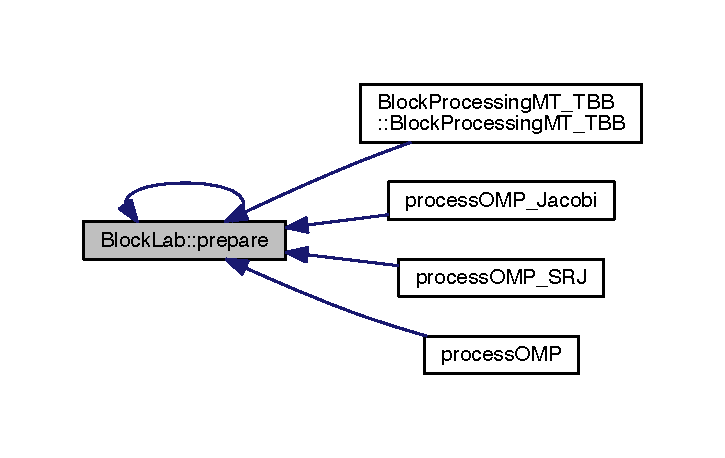
\includegraphics[width=348pt]{d7/d95/class_block_lab_ad529f8c851da336419ad63c25ba76429_icgraph}
\end{center}
\end{figure}


\hypertarget{class_block_lab_ac6236e1c94d13fa1025c8253b9855a04}{}\index{Block\+Lab@{Block\+Lab}!prepare@{prepare}}
\index{prepare@{prepare}!Block\+Lab@{Block\+Lab}}
\subsubsection[{prepare}]{\setlength{\rightskip}{0pt plus 5cm}template$<$typename T\+Block, template$<$ typename X $>$ class allocator = std\+::allocator, typename Element\+Type\+T = typename T\+Block\+::\+Element\+Type$>$ void {\bf Block\+Lab}$<$ T\+Block, allocator, Element\+Type\+T $>$\+::prepare (
\begin{DoxyParamCaption}
\item[{{\bf Grid}$<$ {\bf Block\+Type}, allocator $>$ \&}]{grid, }
\item[{const int}]{stencil\+\_\+start\mbox{[}3\mbox{]}, }
\item[{const int}]{stencil\+\_\+end\mbox{[}3\mbox{]}, }
\item[{const bool}]{istensorial}
\end{DoxyParamCaption}
)\hspace{0.3cm}{\ttfamily [inline]}}\label{class_block_lab_ac6236e1c94d13fa1025c8253b9855a04}
Prepare the extended block. 
\begin{DoxyParams}{Parameters}
{\em collection} & Collection of blocks in the grid (e.\+g. result of Grid\+::get\+Block\+Collection()). \\
\hline
{\em boundary\+Info} & Info on the boundaries of the grid (e.\+g. result of Grid\+::get\+Boundary\+Info()). \\
\hline
{\em stencil\+\_\+start} & Maximal stencil used for computations at lower boundary. Defines how many ghosts we will get in extended block. \\
\hline
{\em stencil\+\_\+end} & Maximal stencil used for computations at lower boundary. Defines how many ghosts we will get in extended block. \\
\hline
\end{DoxyParams}
\hypertarget{class_block_lab_a3e06d4124f7d69923b4ee6345c105cfc}{}\index{Block\+Lab@{Block\+Lab}!read@{read}}
\index{read@{read}!Block\+Lab@{Block\+Lab}}
\subsubsection[{read}]{\setlength{\rightskip}{0pt plus 5cm}template$<$typename T\+Block, template$<$ typename X $>$ class allocator = std\+::allocator, typename Element\+Type\+T = typename T\+Block\+::\+Element\+Type$>$ const {\bf Element\+Type}\& {\bf Block\+Lab}$<$ T\+Block, allocator, Element\+Type\+T $>$\+::read (
\begin{DoxyParamCaption}
\item[{int}]{ix, }
\item[{int}]{iy = {\ttfamily 0}, }
\item[{int}]{iz = {\ttfamily 0}}
\end{DoxyParamCaption}
) const\hspace{0.3cm}{\ttfamily [inline]}}\label{class_block_lab_a3e06d4124f7d69923b4ee6345c105cfc}
Just as Block\+Lab\+::operator() but returning a const. 

\subsection{Member Data Documentation}
\hypertarget{class_block_lab_ade306bb6935a0ead765444534c2e05db}{}\index{Block\+Lab@{Block\+Lab}!istensorial@{istensorial}}
\index{istensorial@{istensorial}!Block\+Lab@{Block\+Lab}}
\subsubsection[{istensorial}]{\setlength{\rightskip}{0pt plus 5cm}template$<$typename T\+Block, template$<$ typename X $>$ class allocator = std\+::allocator, typename Element\+Type\+T = typename T\+Block\+::\+Element\+Type$>$ bool {\bf Block\+Lab}$<$ T\+Block, allocator, Element\+Type\+T $>$\+::istensorial\hspace{0.3cm}{\ttfamily [protected]}}\label{class_block_lab_ade306bb6935a0ead765444534c2e05db}
\hypertarget{class_block_lab_aa6a4c4e00a9bb5ca5780d820b146485b}{}\index{Block\+Lab@{Block\+Lab}!m\+\_\+cache\+Block@{m\+\_\+cache\+Block}}
\index{m\+\_\+cache\+Block@{m\+\_\+cache\+Block}!Block\+Lab@{Block\+Lab}}
\subsubsection[{m\+\_\+cache\+Block}]{\setlength{\rightskip}{0pt plus 5cm}template$<$typename T\+Block, template$<$ typename X $>$ class allocator = std\+::allocator, typename Element\+Type\+T = typename T\+Block\+::\+Element\+Type$>$ {\bf Matrix3\+D}$<${\bf Element\+Type}, true, allocator$>$$\ast$ {\bf Block\+Lab}$<$ T\+Block, allocator, Element\+Type\+T $>$\+::m\+\_\+cache\+Block\hspace{0.3cm}{\ttfamily [protected]}}\label{class_block_lab_aa6a4c4e00a9bb5ca5780d820b146485b}
\hypertarget{class_block_lab_acccfe85f166f20526118fce09b28fb04}{}\index{Block\+Lab@{Block\+Lab}!m\+\_\+ref\+Grid@{m\+\_\+ref\+Grid}}
\index{m\+\_\+ref\+Grid@{m\+\_\+ref\+Grid}!Block\+Lab@{Block\+Lab}}
\subsubsection[{m\+\_\+ref\+Grid}]{\setlength{\rightskip}{0pt plus 5cm}template$<$typename T\+Block, template$<$ typename X $>$ class allocator = std\+::allocator, typename Element\+Type\+T = typename T\+Block\+::\+Element\+Type$>$ const {\bf Grid}$<${\bf Block\+Type}, allocator$>$$\ast$ {\bf Block\+Lab}$<$ T\+Block, allocator, Element\+Type\+T $>$\+::m\+\_\+ref\+Grid\hspace{0.3cm}{\ttfamily [protected]}}\label{class_block_lab_acccfe85f166f20526118fce09b28fb04}
\hypertarget{class_block_lab_a0e11603d73ab4923e1d9033edccdb572}{}\index{Block\+Lab@{Block\+Lab}!m\+\_\+state@{m\+\_\+state}}
\index{m\+\_\+state@{m\+\_\+state}!Block\+Lab@{Block\+Lab}}
\subsubsection[{m\+\_\+state}]{\setlength{\rightskip}{0pt plus 5cm}template$<$typename T\+Block, template$<$ typename X $>$ class allocator = std\+::allocator, typename Element\+Type\+T = typename T\+Block\+::\+Element\+Type$>$ {\bf e\+Block\+Lab\+\_\+\+State} {\bf Block\+Lab}$<$ T\+Block, allocator, Element\+Type\+T $>$\+::m\+\_\+state\hspace{0.3cm}{\ttfamily [protected]}}\label{class_block_lab_a0e11603d73ab4923e1d9033edccdb572}
\hypertarget{class_block_lab_a46fee08b49b11be489c71f726e258cc9}{}\index{Block\+Lab@{Block\+Lab}!m\+\_\+stencil\+End@{m\+\_\+stencil\+End}}
\index{m\+\_\+stencil\+End@{m\+\_\+stencil\+End}!Block\+Lab@{Block\+Lab}}
\subsubsection[{m\+\_\+stencil\+End}]{\setlength{\rightskip}{0pt plus 5cm}template$<$typename T\+Block, template$<$ typename X $>$ class allocator = std\+::allocator, typename Element\+Type\+T = typename T\+Block\+::\+Element\+Type$>$ int {\bf Block\+Lab}$<$ T\+Block, allocator, Element\+Type\+T $>$\+::m\+\_\+stencil\+End\mbox{[}3\mbox{]}\hspace{0.3cm}{\ttfamily [protected]}}\label{class_block_lab_a46fee08b49b11be489c71f726e258cc9}
\hypertarget{class_block_lab_a8ac6690f98ba84346a74b5b95c3afb2b}{}\index{Block\+Lab@{Block\+Lab}!m\+\_\+stencil\+Start@{m\+\_\+stencil\+Start}}
\index{m\+\_\+stencil\+Start@{m\+\_\+stencil\+Start}!Block\+Lab@{Block\+Lab}}
\subsubsection[{m\+\_\+stencil\+Start}]{\setlength{\rightskip}{0pt plus 5cm}template$<$typename T\+Block, template$<$ typename X $>$ class allocator = std\+::allocator, typename Element\+Type\+T = typename T\+Block\+::\+Element\+Type$>$ int {\bf Block\+Lab}$<$ T\+Block, allocator, Element\+Type\+T $>$\+::m\+\_\+stencil\+Start\mbox{[}3\mbox{]}\hspace{0.3cm}{\ttfamily [protected]}}\label{class_block_lab_a8ac6690f98ba84346a74b5b95c3afb2b}
\hypertarget{class_block_lab_abcd7367c6f45124d3202c8da5043ac93}{}\index{Block\+Lab@{Block\+Lab}!N\+X@{N\+X}}
\index{N\+X@{N\+X}!Block\+Lab@{Block\+Lab}}
\subsubsection[{N\+X}]{\setlength{\rightskip}{0pt plus 5cm}template$<$typename T\+Block, template$<$ typename X $>$ class allocator = std\+::allocator, typename Element\+Type\+T = typename T\+Block\+::\+Element\+Type$>$ int {\bf Block\+Lab}$<$ T\+Block, allocator, Element\+Type\+T $>$\+::N\+X\hspace{0.3cm}{\ttfamily [protected]}}\label{class_block_lab_abcd7367c6f45124d3202c8da5043ac93}
\hypertarget{class_block_lab_aaa1e748664ebb6b4fc7c47cf30a445db}{}\index{Block\+Lab@{Block\+Lab}!N\+Y@{N\+Y}}
\index{N\+Y@{N\+Y}!Block\+Lab@{Block\+Lab}}
\subsubsection[{N\+Y}]{\setlength{\rightskip}{0pt plus 5cm}template$<$typename T\+Block, template$<$ typename X $>$ class allocator = std\+::allocator, typename Element\+Type\+T = typename T\+Block\+::\+Element\+Type$>$ int {\bf Block\+Lab}$<$ T\+Block, allocator, Element\+Type\+T $>$\+::N\+Y\hspace{0.3cm}{\ttfamily [protected]}}\label{class_block_lab_aaa1e748664ebb6b4fc7c47cf30a445db}
\hypertarget{class_block_lab_acdd7f4e2489d31da6a2a76099807a7c5}{}\index{Block\+Lab@{Block\+Lab}!N\+Z@{N\+Z}}
\index{N\+Z@{N\+Z}!Block\+Lab@{Block\+Lab}}
\subsubsection[{N\+Z}]{\setlength{\rightskip}{0pt plus 5cm}template$<$typename T\+Block, template$<$ typename X $>$ class allocator = std\+::allocator, typename Element\+Type\+T = typename T\+Block\+::\+Element\+Type$>$ int {\bf Block\+Lab}$<$ T\+Block, allocator, Element\+Type\+T $>$\+::N\+Z\hspace{0.3cm}{\ttfamily [protected]}}\label{class_block_lab_acdd7f4e2489d31da6a2a76099807a7c5}


The documentation for this class was generated from the following file\+:\begin{DoxyCompactItemize}
\item 
Cubism/\hyperlink{_block_lab_8h}{Block\+Lab.\+h}\end{DoxyCompactItemize}

\hypertarget{class_block_lab_box}{}\section{Block\+Lab\+Box$<$ Block\+Type, allocator $>$ Class Template Reference}
\label{class_block_lab_box}\index{Block\+Lab\+Box$<$ Block\+Type, allocator $>$@{Block\+Lab\+Box$<$ Block\+Type, allocator $>$}}


{\ttfamily \#include $<$Definitions.\+h$>$}



Inheritance diagram for Block\+Lab\+Box$<$ Block\+Type, allocator $>$\+:\nopagebreak
\begin{figure}[H]
\begin{center}
\leavevmode
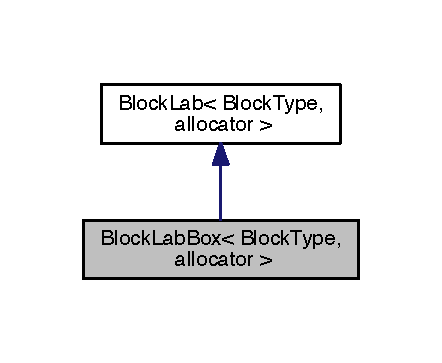
\includegraphics[width=212pt]{d8/d35/class_block_lab_box__inherit__graph}
\end{center}
\end{figure}


Collaboration diagram for Block\+Lab\+Box$<$ Block\+Type, allocator $>$\+:\nopagebreak
\begin{figure}[H]
\begin{center}
\leavevmode
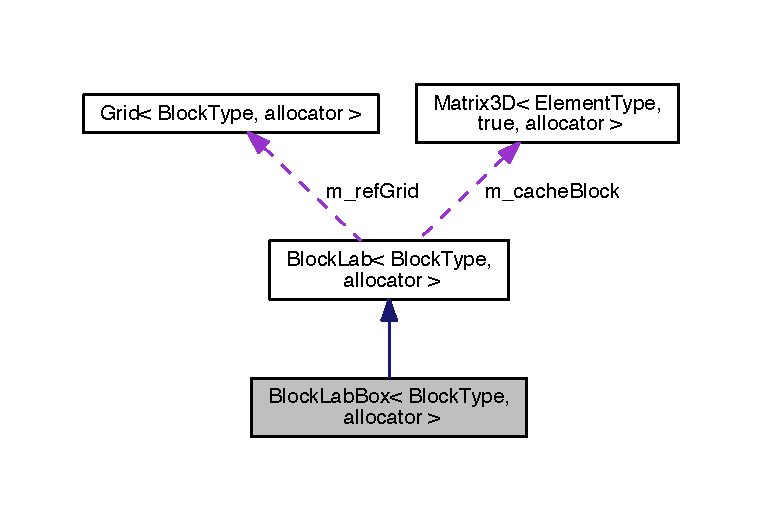
\includegraphics[width=350pt]{d0/d61/class_block_lab_box__coll__graph}
\end{center}
\end{figure}
\subsection*{Public Member Functions}
\begin{DoxyCompactItemize}
\item 
\hyperlink{class_block_lab_box_a819b297579990253484d7fed5dc878db}{Block\+Lab\+Box} ()
\item 
void \hyperlink{class_block_lab_box_adfd9b3d46062be59f03d0c1df79db81d}{\+\_\+apply\+\_\+bc} (const \hyperlink{struct_block_info}{Block\+Info} \&info, const \hyperlink{_h_d_f5_dumper_8h_a445a5f0e2a34c9d97d69a3c2d1957907}{Real} t=0)
\end{DoxyCompactItemize}
\subsection*{Additional Inherited Members}


\subsection{Constructor \& Destructor Documentation}
\hypertarget{class_block_lab_box_a819b297579990253484d7fed5dc878db}{}\index{Block\+Lab\+Box@{Block\+Lab\+Box}!Block\+Lab\+Box@{Block\+Lab\+Box}}
\index{Block\+Lab\+Box@{Block\+Lab\+Box}!Block\+Lab\+Box@{Block\+Lab\+Box}}
\subsubsection[{Block\+Lab\+Box}]{\setlength{\rightskip}{0pt plus 5cm}template$<$typename Block\+Type , template$<$ typename X $>$ class allocator = std\+::allocator$>$ {\bf Block\+Lab\+Box}$<$ {\bf Block\+Type}, allocator $>$\+::{\bf Block\+Lab\+Box} (
\begin{DoxyParamCaption}
{}
\end{DoxyParamCaption}
)\hspace{0.3cm}{\ttfamily [inline]}}\label{class_block_lab_box_a819b297579990253484d7fed5dc878db}


\subsection{Member Function Documentation}
\hypertarget{class_block_lab_box_adfd9b3d46062be59f03d0c1df79db81d}{}\index{Block\+Lab\+Box@{Block\+Lab\+Box}!\+\_\+apply\+\_\+bc@{\+\_\+apply\+\_\+bc}}
\index{\+\_\+apply\+\_\+bc@{\+\_\+apply\+\_\+bc}!Block\+Lab\+Box@{Block\+Lab\+Box}}
\subsubsection[{\+\_\+apply\+\_\+bc}]{\setlength{\rightskip}{0pt plus 5cm}template$<$typename Block\+Type , template$<$ typename X $>$ class allocator = std\+::allocator$>$ void {\bf Block\+Lab\+Box}$<$ {\bf Block\+Type}, allocator $>$\+::\+\_\+apply\+\_\+bc (
\begin{DoxyParamCaption}
\item[{const {\bf Block\+Info} \&}]{info, }
\item[{const {\bf Real}}]{t = {\ttfamily 0}}
\end{DoxyParamCaption}
)\hspace{0.3cm}{\ttfamily [inline]}, {\ttfamily [virtual]}}\label{class_block_lab_box_adfd9b3d46062be59f03d0c1df79db81d}


Reimplemented from \hyperlink{class_block_lab_a669ac139b57be4967e5f43bc649a8520}{Block\+Lab$<$ Block\+Type, allocator $>$}.



The documentation for this class was generated from the following file\+:\begin{DoxyCompactItemize}
\item 
/\+Users/cconti/\+Desktop/\+Mounts/\+Brutus\+Home/\+Cubism\+U\+P\+\_\+2\+D/source/\hyperlink{_definitions_8h}{Definitions.\+h}\end{DoxyCompactItemize}

\hypertarget{class_block_lab_dirichlet}{}\section{Block\+Lab\+Dirichlet$<$ Block\+Type, allocator $>$ Class Template Reference}
\label{class_block_lab_dirichlet}\index{Block\+Lab\+Dirichlet$<$ Block\+Type, allocator $>$@{Block\+Lab\+Dirichlet$<$ Block\+Type, allocator $>$}}


{\ttfamily \#include $<$Definitions.\+h$>$}



Inheritance diagram for Block\+Lab\+Dirichlet$<$ Block\+Type, allocator $>$\+:\nopagebreak
\begin{figure}[H]
\begin{center}
\leavevmode
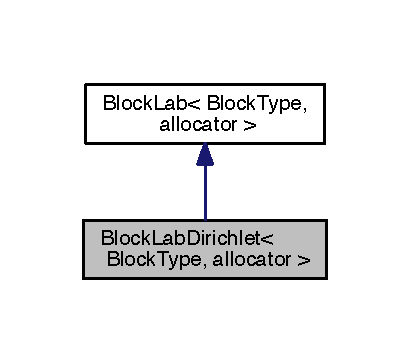
\includegraphics[width=197pt]{d6/d91/class_block_lab_dirichlet__inherit__graph}
\end{center}
\end{figure}


Collaboration diagram for Block\+Lab\+Dirichlet$<$ Block\+Type, allocator $>$\+:\nopagebreak
\begin{figure}[H]
\begin{center}
\leavevmode
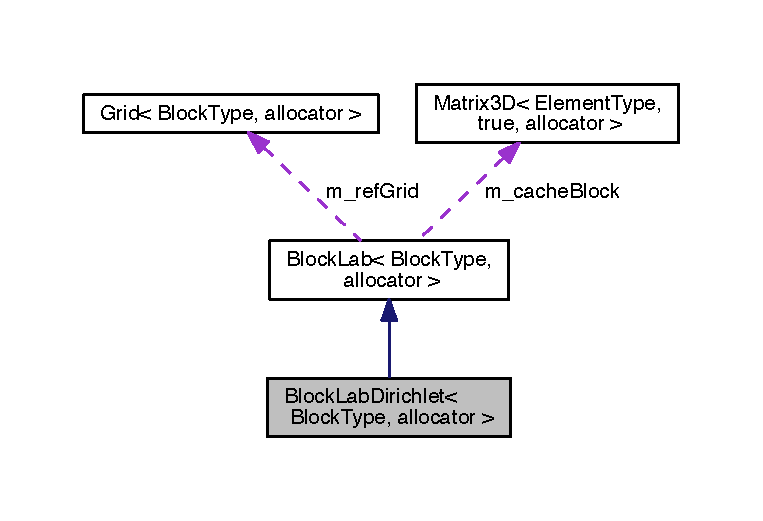
\includegraphics[width=350pt]{dc/dfc/class_block_lab_dirichlet__coll__graph}
\end{center}
\end{figure}
\subsection*{Public Member Functions}
\begin{DoxyCompactItemize}
\item 
\hyperlink{class_block_lab_dirichlet_aee522a1b0a5e8047dea4558b34df6141}{Block\+Lab\+Dirichlet} ()
\item 
void \hyperlink{class_block_lab_dirichlet_ae05580142a8ddb65c42fd92063355609}{\+\_\+apply\+\_\+bc} (const \hyperlink{struct_block_info}{Block\+Info} \&info, const \hyperlink{_h_d_f5_dumper_8h_a445a5f0e2a34c9d97d69a3c2d1957907}{Real} t=0)
\end{DoxyCompactItemize}
\subsection*{Additional Inherited Members}


\subsection{Constructor \& Destructor Documentation}
\hypertarget{class_block_lab_dirichlet_aee522a1b0a5e8047dea4558b34df6141}{}\index{Block\+Lab\+Dirichlet@{Block\+Lab\+Dirichlet}!Block\+Lab\+Dirichlet@{Block\+Lab\+Dirichlet}}
\index{Block\+Lab\+Dirichlet@{Block\+Lab\+Dirichlet}!Block\+Lab\+Dirichlet@{Block\+Lab\+Dirichlet}}
\subsubsection[{Block\+Lab\+Dirichlet}]{\setlength{\rightskip}{0pt plus 5cm}template$<$typename Block\+Type , template$<$ typename X $>$ class allocator = std\+::allocator$>$ {\bf Block\+Lab\+Dirichlet}$<$ {\bf Block\+Type}, allocator $>$\+::{\bf Block\+Lab\+Dirichlet} (
\begin{DoxyParamCaption}
{}
\end{DoxyParamCaption}
)\hspace{0.3cm}{\ttfamily [inline]}}\label{class_block_lab_dirichlet_aee522a1b0a5e8047dea4558b34df6141}


\subsection{Member Function Documentation}
\hypertarget{class_block_lab_dirichlet_ae05580142a8ddb65c42fd92063355609}{}\index{Block\+Lab\+Dirichlet@{Block\+Lab\+Dirichlet}!\+\_\+apply\+\_\+bc@{\+\_\+apply\+\_\+bc}}
\index{\+\_\+apply\+\_\+bc@{\+\_\+apply\+\_\+bc}!Block\+Lab\+Dirichlet@{Block\+Lab\+Dirichlet}}
\subsubsection[{\+\_\+apply\+\_\+bc}]{\setlength{\rightskip}{0pt plus 5cm}template$<$typename Block\+Type , template$<$ typename X $>$ class allocator = std\+::allocator$>$ void {\bf Block\+Lab\+Dirichlet}$<$ {\bf Block\+Type}, allocator $>$\+::\+\_\+apply\+\_\+bc (
\begin{DoxyParamCaption}
\item[{const {\bf Block\+Info} \&}]{info, }
\item[{const {\bf Real}}]{t = {\ttfamily 0}}
\end{DoxyParamCaption}
)\hspace{0.3cm}{\ttfamily [inline]}, {\ttfamily [virtual]}}\label{class_block_lab_dirichlet_ae05580142a8ddb65c42fd92063355609}


Reimplemented from \hyperlink{class_block_lab_a669ac139b57be4967e5f43bc649a8520}{Block\+Lab$<$ Block\+Type, allocator $>$}.



The documentation for this class was generated from the following file\+:\begin{DoxyCompactItemize}
\item 
source/\hyperlink{_definitions_8h}{Definitions.\+h}\end{DoxyCompactItemize}

\hypertarget{class_block_lab_m_p_i}{}\section{Block\+Lab\+M\+P\+I$<$ My\+Block\+Lab $>$ Class Template Reference}
\label{class_block_lab_m_p_i}\index{Block\+Lab\+M\+P\+I$<$ My\+Block\+Lab $>$@{Block\+Lab\+M\+P\+I$<$ My\+Block\+Lab $>$}}


{\ttfamily \#include $<$Block\+Lab\+M\+P\+I.\+h$>$}



Inheritance diagram for Block\+Lab\+M\+P\+I$<$ My\+Block\+Lab $>$\+:
% FIG 0


Collaboration diagram for Block\+Lab\+M\+P\+I$<$ My\+Block\+Lab $>$\+:
% FIG 1
\subsection*{Public Member Functions}
\begin{DoxyCompactItemize}
\item 
{\footnotesize template$<$typename T\+Grid $>$ }\\void \hyperlink{class_block_lab_m_p_i_a49e9b846d16c1c3f177b6ff067bc791c}{prepare} (\hyperlink{class_grid_m_p_i}{Grid\+M\+P\+I}$<$ T\+Grid $>$ \&grid, const \hyperlink{class_synchronizer_m_p_i}{Synchronizer\+M\+P\+I} \&\hyperlink{class_synchronizer_m_p_i}{Synchronizer\+M\+P\+I})
\item 
void \hyperlink{class_block_lab_m_p_i_a9695a460545974a0aa473039c3876765}{load} (const \hyperlink{struct_block_info}{Block\+Info} \&info, const \hyperlink{_h_d_f5_dumper_8h_a445a5f0e2a34c9d97d69a3c2d1957907}{Real} t=0, const bool applybc=true)
\end{DoxyCompactItemize}
\subsection*{Protected Attributes}
\begin{DoxyCompactItemize}
\item 
int \hyperlink{class_block_lab_m_p_i_a346371e08c48393a09a60188aa210828}{mypeindex} \mbox{[}3\mbox{]}
\item 
int \hyperlink{class_block_lab_m_p_i_a3c58102452df2ae20110af79d504693e}{pesize} \mbox{[}3\mbox{]}
\item 
int \hyperlink{class_block_lab_m_p_i_a11a592341f9c28f07809f0d950512fe5}{mybpd} \mbox{[}3\mbox{]}
\item 
int \hyperlink{class_block_lab_m_p_i_a41646b94f197315e4c39c5155ee939eb}{g\+Last\+X}
\item 
int \hyperlink{class_block_lab_m_p_i_afc336a0d08b78a9196eb24701816d6c8}{g\+Last\+Y}
\item 
int \hyperlink{class_block_lab_m_p_i_a8b9247a3ec2caad18896f597b98b7103}{g\+Last\+Z}
\end{DoxyCompactItemize}


\subsection{Member Function Documentation}
\hypertarget{class_block_lab_m_p_i_a9695a460545974a0aa473039c3876765}{}\index{Block\+Lab\+M\+P\+I@{Block\+Lab\+M\+P\+I}!load@{load}}
\index{load@{load}!Block\+Lab\+M\+P\+I@{Block\+Lab\+M\+P\+I}}
\subsubsection[{load}]{\setlength{\rightskip}{0pt plus 5cm}template$<$typename My\+Block\+Lab $>$ void {\bf Block\+Lab\+M\+P\+I}$<$ My\+Block\+Lab $>$\+::load (
\begin{DoxyParamCaption}
\item[{const {\bf Block\+Info} \&}]{info, }
\item[{const {\bf Real}}]{t = {\ttfamily 0}, }
\item[{const bool}]{applybc = {\ttfamily true}}
\end{DoxyParamCaption}
)\hspace{0.3cm}{\ttfamily [inline]}}\label{class_block_lab_m_p_i_a9695a460545974a0aa473039c3876765}


Here is the call graph for this function\+:
% FIG 2


\hypertarget{class_block_lab_m_p_i_a49e9b846d16c1c3f177b6ff067bc791c}{}\index{Block\+Lab\+M\+P\+I@{Block\+Lab\+M\+P\+I}!prepare@{prepare}}
\index{prepare@{prepare}!Block\+Lab\+M\+P\+I@{Block\+Lab\+M\+P\+I}}
\subsubsection[{prepare}]{\setlength{\rightskip}{0pt plus 5cm}template$<$typename My\+Block\+Lab $>$ template$<$typename T\+Grid $>$ void {\bf Block\+Lab\+M\+P\+I}$<$ My\+Block\+Lab $>$\+::prepare (
\begin{DoxyParamCaption}
\item[{{\bf Grid\+M\+P\+I}$<$ T\+Grid $>$ \&}]{grid, }
\item[{const {\bf Synchronizer\+M\+P\+I} \&}]{Synchronizer\+M\+P\+I}
\end{DoxyParamCaption}
)\hspace{0.3cm}{\ttfamily [inline]}}\label{class_block_lab_m_p_i_a49e9b846d16c1c3f177b6ff067bc791c}


Here is the call graph for this function\+:
% FIG 3




\subsection{Member Data Documentation}
\hypertarget{class_block_lab_m_p_i_a41646b94f197315e4c39c5155ee939eb}{}\index{Block\+Lab\+M\+P\+I@{Block\+Lab\+M\+P\+I}!g\+Last\+X@{g\+Last\+X}}
\index{g\+Last\+X@{g\+Last\+X}!Block\+Lab\+M\+P\+I@{Block\+Lab\+M\+P\+I}}
\subsubsection[{g\+Last\+X}]{\setlength{\rightskip}{0pt plus 5cm}template$<$typename My\+Block\+Lab $>$ int {\bf Block\+Lab\+M\+P\+I}$<$ My\+Block\+Lab $>$\+::g\+Last\+X\hspace{0.3cm}{\ttfamily [protected]}}\label{class_block_lab_m_p_i_a41646b94f197315e4c39c5155ee939eb}
\hypertarget{class_block_lab_m_p_i_afc336a0d08b78a9196eb24701816d6c8}{}\index{Block\+Lab\+M\+P\+I@{Block\+Lab\+M\+P\+I}!g\+Last\+Y@{g\+Last\+Y}}
\index{g\+Last\+Y@{g\+Last\+Y}!Block\+Lab\+M\+P\+I@{Block\+Lab\+M\+P\+I}}
\subsubsection[{g\+Last\+Y}]{\setlength{\rightskip}{0pt plus 5cm}template$<$typename My\+Block\+Lab $>$ int {\bf Block\+Lab\+M\+P\+I}$<$ My\+Block\+Lab $>$\+::g\+Last\+Y\hspace{0.3cm}{\ttfamily [protected]}}\label{class_block_lab_m_p_i_afc336a0d08b78a9196eb24701816d6c8}
\hypertarget{class_block_lab_m_p_i_a8b9247a3ec2caad18896f597b98b7103}{}\index{Block\+Lab\+M\+P\+I@{Block\+Lab\+M\+P\+I}!g\+Last\+Z@{g\+Last\+Z}}
\index{g\+Last\+Z@{g\+Last\+Z}!Block\+Lab\+M\+P\+I@{Block\+Lab\+M\+P\+I}}
\subsubsection[{g\+Last\+Z}]{\setlength{\rightskip}{0pt plus 5cm}template$<$typename My\+Block\+Lab $>$ int {\bf Block\+Lab\+M\+P\+I}$<$ My\+Block\+Lab $>$\+::g\+Last\+Z\hspace{0.3cm}{\ttfamily [protected]}}\label{class_block_lab_m_p_i_a8b9247a3ec2caad18896f597b98b7103}
\hypertarget{class_block_lab_m_p_i_a11a592341f9c28f07809f0d950512fe5}{}\index{Block\+Lab\+M\+P\+I@{Block\+Lab\+M\+P\+I}!mybpd@{mybpd}}
\index{mybpd@{mybpd}!Block\+Lab\+M\+P\+I@{Block\+Lab\+M\+P\+I}}
\subsubsection[{mybpd}]{\setlength{\rightskip}{0pt plus 5cm}template$<$typename My\+Block\+Lab $>$ int {\bf Block\+Lab\+M\+P\+I}$<$ My\+Block\+Lab $>$\+::mybpd\mbox{[}3\mbox{]}\hspace{0.3cm}{\ttfamily [protected]}}\label{class_block_lab_m_p_i_a11a592341f9c28f07809f0d950512fe5}
\hypertarget{class_block_lab_m_p_i_a346371e08c48393a09a60188aa210828}{}\index{Block\+Lab\+M\+P\+I@{Block\+Lab\+M\+P\+I}!mypeindex@{mypeindex}}
\index{mypeindex@{mypeindex}!Block\+Lab\+M\+P\+I@{Block\+Lab\+M\+P\+I}}
\subsubsection[{mypeindex}]{\setlength{\rightskip}{0pt plus 5cm}template$<$typename My\+Block\+Lab $>$ int {\bf Block\+Lab\+M\+P\+I}$<$ My\+Block\+Lab $>$\+::mypeindex\mbox{[}3\mbox{]}\hspace{0.3cm}{\ttfamily [protected]}}\label{class_block_lab_m_p_i_a346371e08c48393a09a60188aa210828}
\hypertarget{class_block_lab_m_p_i_a3c58102452df2ae20110af79d504693e}{}\index{Block\+Lab\+M\+P\+I@{Block\+Lab\+M\+P\+I}!pesize@{pesize}}
\index{pesize@{pesize}!Block\+Lab\+M\+P\+I@{Block\+Lab\+M\+P\+I}}
\subsubsection[{pesize}]{\setlength{\rightskip}{0pt plus 5cm}template$<$typename My\+Block\+Lab $>$ int {\bf Block\+Lab\+M\+P\+I}$<$ My\+Block\+Lab $>$\+::pesize\mbox{[}3\mbox{]}\hspace{0.3cm}{\ttfamily [protected]}}\label{class_block_lab_m_p_i_a3c58102452df2ae20110af79d504693e}


The documentation for this class was generated from the following file\+:\begin{DoxyCompactItemize}
\item 
/\+Users/cconti/\+Desktop/\+Mounts/\+Brutus\+Home/\+Seed/\+Cubism\+U\+P\+\_\+2\+D/\+Cubism/\hyperlink{_block_lab_m_p_i_8h}{Block\+Lab\+M\+P\+I.\+h}\end{DoxyCompactItemize}

\hypertarget{class_block_lab_neumann}{}\section{Block\+Lab\+Neumann$<$ Block\+Type, allocator $>$ Class Template Reference}
\label{class_block_lab_neumann}\index{Block\+Lab\+Neumann$<$ Block\+Type, allocator $>$@{Block\+Lab\+Neumann$<$ Block\+Type, allocator $>$}}


{\ttfamily \#include $<$Definitions.\+h$>$}



Inheritance diagram for Block\+Lab\+Neumann$<$ Block\+Type, allocator $>$\+:
% FIG 0


Collaboration diagram for Block\+Lab\+Neumann$<$ Block\+Type, allocator $>$\+:
% FIG 1
\subsection*{Public Member Functions}
\begin{DoxyCompactItemize}
\item 
\hyperlink{class_block_lab_neumann_ab365064c3cc0d442c730d90cd8c5bd0b}{Block\+Lab\+Neumann} ()
\item 
void \hyperlink{class_block_lab_neumann_a65cd80126a426fa2aa098910fd189793}{\+\_\+apply\+\_\+bc} (const \hyperlink{struct_block_info}{Block\+Info} \&info, const \hyperlink{_h_d_f5_dumper_8h_a445a5f0e2a34c9d97d69a3c2d1957907}{Real} t=0)
\end{DoxyCompactItemize}
\subsection*{Additional Inherited Members}


\subsection{Constructor \& Destructor Documentation}
\hypertarget{class_block_lab_neumann_ab365064c3cc0d442c730d90cd8c5bd0b}{}\index{Block\+Lab\+Neumann@{Block\+Lab\+Neumann}!Block\+Lab\+Neumann@{Block\+Lab\+Neumann}}
\index{Block\+Lab\+Neumann@{Block\+Lab\+Neumann}!Block\+Lab\+Neumann@{Block\+Lab\+Neumann}}
\subsubsection[{Block\+Lab\+Neumann}]{\setlength{\rightskip}{0pt plus 5cm}template$<$typename Block\+Type , template$<$ typename X $>$ class allocator = std\+::allocator$>$ {\bf Block\+Lab\+Neumann}$<$ {\bf Block\+Type}, allocator $>$\+::{\bf Block\+Lab\+Neumann} (
\begin{DoxyParamCaption}
{}
\end{DoxyParamCaption}
)\hspace{0.3cm}{\ttfamily [inline]}}\label{class_block_lab_neumann_ab365064c3cc0d442c730d90cd8c5bd0b}


\subsection{Member Function Documentation}
\hypertarget{class_block_lab_neumann_a65cd80126a426fa2aa098910fd189793}{}\index{Block\+Lab\+Neumann@{Block\+Lab\+Neumann}!\+\_\+apply\+\_\+bc@{\+\_\+apply\+\_\+bc}}
\index{\+\_\+apply\+\_\+bc@{\+\_\+apply\+\_\+bc}!Block\+Lab\+Neumann@{Block\+Lab\+Neumann}}
\subsubsection[{\+\_\+apply\+\_\+bc}]{\setlength{\rightskip}{0pt plus 5cm}template$<$typename Block\+Type , template$<$ typename X $>$ class allocator = std\+::allocator$>$ void {\bf Block\+Lab\+Neumann}$<$ {\bf Block\+Type}, allocator $>$\+::\+\_\+apply\+\_\+bc (
\begin{DoxyParamCaption}
\item[{const {\bf Block\+Info} \&}]{info, }
\item[{const {\bf Real}}]{t = {\ttfamily 0}}
\end{DoxyParamCaption}
)\hspace{0.3cm}{\ttfamily [inline]}, {\ttfamily [virtual]}}\label{class_block_lab_neumann_a65cd80126a426fa2aa098910fd189793}


Reimplemented from \hyperlink{class_block_lab_a669ac139b57be4967e5f43bc649a8520}{Block\+Lab$<$ Block\+Type, allocator $>$}.



The documentation for this class was generated from the following file\+:\begin{DoxyCompactItemize}
\item 
/\+Users/cconti/\+Desktop/\+Mounts/\+Brutus\+Home/\+Seed/\+Cubism\+U\+P\+\_\+2\+D/source/\hyperlink{_definitions_8h}{Definitions.\+h}\end{DoxyCompactItemize}

\hypertarget{class_block_processing___t_b_b}{}\section{Block\+Processing\+\_\+\+T\+B\+B$<$ Block\+Type $>$ Class Template Reference}
\label{class_block_processing___t_b_b}\index{Block\+Processing\+\_\+\+T\+B\+B$<$ Block\+Type $>$@{Block\+Processing\+\_\+\+T\+B\+B$<$ Block\+Type $>$}}


{\ttfamily \#include $<$Block\+Processing.\+h$>$}

\subsection*{Public Member Functions}
\begin{DoxyCompactItemize}
\item 
\hyperlink{class_block_processing___t_b_b_a1a3d202984fe1c763a1d3a60ed1c8da8}{Block\+Processing\+\_\+\+T\+B\+B} ()
\item 
virtual \hyperlink{class_block_processing___t_b_b_a00a2d6deca06bc723a0e6fbffc0a3a6c}{$\sim$\+Block\+Processing\+\_\+\+T\+B\+B} ()
\end{DoxyCompactItemize}
\subsection*{Static Public Member Functions}
\begin{DoxyCompactItemize}
\item 
{\footnotesize template$<$typename Processing , typename Grid $>$ }\\static void \hyperlink{class_block_processing___t_b_b_afb4ac5aee8af3d4e9f3a0f572bdd0a04}{process} (vector$<$ \hyperlink{struct_block_info}{Block\+Info} $>$ \&v\+Info, Processing \&p, \hyperlink{class_grid}{Grid} \&grid, int n\+Granularity=-\/1)
\item 
{\footnotesize template$<$typename Lab , typename Grid , typename Processing $>$ }\\static void \hyperlink{class_block_processing___t_b_b_a19d9699a50fba9a15eca0e0e1a7f1efd}{process} (vector$<$ \hyperlink{struct_block_info}{Block\+Info} $>$ \&v\+Info, Processing \&p, \hyperlink{class_grid}{Grid} \&grid, const \hyperlink{_h_d_f5_dumper_8h_a445a5f0e2a34c9d97d69a3c2d1957907}{Real} t=0, const bool tensorial=false, int n\+Granularity=-\/1)
\end{DoxyCompactItemize}
\subsection*{Static Protected Member Functions}
\begin{DoxyCompactItemize}
\item 
{\footnotesize template$<$typename Lab $>$ }\\static void \hyperlink{class_block_processing___t_b_b_a4a77964ec9a1bbf0054f4e5e511ae8ea}{\+\_\+get\+Resources} (concurrent\+\_\+queue$<$ \hyperlink{_definitions_8h_ad6f951af9a2a6ebc1975404882b34314}{Lab} $\ast$ $>$ \&resources, const int n\+Slots)
\item 
static const \hyperlink{struct_block_info}{Block\+Info} $\ast$ \hyperlink{class_block_processing___t_b_b_a5316cc197b479887abb3c9b74cdf9c31}{\+\_\+prepare\+Block\+Infos} (vector$<$ \hyperlink{struct_block_info}{Block\+Info} $>$ \&v\+Info)
\end{DoxyCompactItemize}


\subsection{Detailed Description}
\subsubsection*{template$<$typename Block\+Type$>$class Block\+Processing\+\_\+\+T\+B\+B$<$ Block\+Type $>$}

Process blocks with tbb (using threads). \begin{DoxySeeAlso}{See also}
\hyperlink{class_block_processing___t_b_b_afb4ac5aee8af3d4e9f3a0f572bdd0a04}{Block\+Processing\+\_\+\+T\+B\+B\+::process} 
\end{DoxySeeAlso}


\subsection{Constructor \& Destructor Documentation}
\hypertarget{class_block_processing___t_b_b_a1a3d202984fe1c763a1d3a60ed1c8da8}{}\index{Block\+Processing\+\_\+\+T\+B\+B@{Block\+Processing\+\_\+\+T\+B\+B}!Block\+Processing\+\_\+\+T\+B\+B@{Block\+Processing\+\_\+\+T\+B\+B}}
\index{Block\+Processing\+\_\+\+T\+B\+B@{Block\+Processing\+\_\+\+T\+B\+B}!Block\+Processing\+\_\+\+T\+B\+B@{Block\+Processing\+\_\+\+T\+B\+B}}
\subsubsection[{Block\+Processing\+\_\+\+T\+B\+B}]{\setlength{\rightskip}{0pt plus 5cm}template$<$typename Block\+Type $>$ {\bf Block\+Processing\+\_\+\+T\+B\+B}$<$ Block\+Type $>$\+::{\bf Block\+Processing\+\_\+\+T\+B\+B} (
\begin{DoxyParamCaption}
{}
\end{DoxyParamCaption}
)\hspace{0.3cm}{\ttfamily [inline]}}\label{class_block_processing___t_b_b_a1a3d202984fe1c763a1d3a60ed1c8da8}
\hypertarget{class_block_processing___t_b_b_a00a2d6deca06bc723a0e6fbffc0a3a6c}{}\index{Block\+Processing\+\_\+\+T\+B\+B@{Block\+Processing\+\_\+\+T\+B\+B}!````~Block\+Processing\+\_\+\+T\+B\+B@{$\sim$\+Block\+Processing\+\_\+\+T\+B\+B}}
\index{````~Block\+Processing\+\_\+\+T\+B\+B@{$\sim$\+Block\+Processing\+\_\+\+T\+B\+B}!Block\+Processing\+\_\+\+T\+B\+B@{Block\+Processing\+\_\+\+T\+B\+B}}
\subsubsection[{$\sim$\+Block\+Processing\+\_\+\+T\+B\+B}]{\setlength{\rightskip}{0pt plus 5cm}template$<$typename Block\+Type $>$ virtual {\bf Block\+Processing\+\_\+\+T\+B\+B}$<$ Block\+Type $>$\+::$\sim${\bf Block\+Processing\+\_\+\+T\+B\+B} (
\begin{DoxyParamCaption}
{}
\end{DoxyParamCaption}
)\hspace{0.3cm}{\ttfamily [inline]}, {\ttfamily [virtual]}}\label{class_block_processing___t_b_b_a00a2d6deca06bc723a0e6fbffc0a3a6c}


\subsection{Member Function Documentation}
\hypertarget{class_block_processing___t_b_b_a4a77964ec9a1bbf0054f4e5e511ae8ea}{}\index{Block\+Processing\+\_\+\+T\+B\+B@{Block\+Processing\+\_\+\+T\+B\+B}!\+\_\+get\+Resources@{\+\_\+get\+Resources}}
\index{\+\_\+get\+Resources@{\+\_\+get\+Resources}!Block\+Processing\+\_\+\+T\+B\+B@{Block\+Processing\+\_\+\+T\+B\+B}}
\subsubsection[{\+\_\+get\+Resources}]{\setlength{\rightskip}{0pt plus 5cm}template$<$typename Block\+Type $>$ template$<$typename Lab $>$ static void {\bf Block\+Processing\+\_\+\+T\+B\+B}$<$ Block\+Type $>$\+::\+\_\+get\+Resources (
\begin{DoxyParamCaption}
\item[{concurrent\+\_\+queue$<$ {\bf Lab} $\ast$ $>$ \&}]{resources, }
\item[{const int}]{n\+Slots}
\end{DoxyParamCaption}
)\hspace{0.3cm}{\ttfamily [inline]}, {\ttfamily [static]}, {\ttfamily [protected]}}\label{class_block_processing___t_b_b_a4a77964ec9a1bbf0054f4e5e511ae8ea}
\hypertarget{class_block_processing___t_b_b_a5316cc197b479887abb3c9b74cdf9c31}{}\index{Block\+Processing\+\_\+\+T\+B\+B@{Block\+Processing\+\_\+\+T\+B\+B}!\+\_\+prepare\+Block\+Infos@{\+\_\+prepare\+Block\+Infos}}
\index{\+\_\+prepare\+Block\+Infos@{\+\_\+prepare\+Block\+Infos}!Block\+Processing\+\_\+\+T\+B\+B@{Block\+Processing\+\_\+\+T\+B\+B}}
\subsubsection[{\+\_\+prepare\+Block\+Infos}]{\setlength{\rightskip}{0pt plus 5cm}template$<$typename Block\+Type $>$ static const {\bf Block\+Info}$\ast$ {\bf Block\+Processing\+\_\+\+T\+B\+B}$<$ Block\+Type $>$\+::\+\_\+prepare\+Block\+Infos (
\begin{DoxyParamCaption}
\item[{vector$<$ {\bf Block\+Info} $>$ \&}]{v\+Info}
\end{DoxyParamCaption}
)\hspace{0.3cm}{\ttfamily [inline]}, {\ttfamily [static]}, {\ttfamily [protected]}}\label{class_block_processing___t_b_b_a5316cc197b479887abb3c9b74cdf9c31}
\hypertarget{class_block_processing___t_b_b_afb4ac5aee8af3d4e9f3a0f572bdd0a04}{}\index{Block\+Processing\+\_\+\+T\+B\+B@{Block\+Processing\+\_\+\+T\+B\+B}!process@{process}}
\index{process@{process}!Block\+Processing\+\_\+\+T\+B\+B@{Block\+Processing\+\_\+\+T\+B\+B}}
\subsubsection[{process}]{\setlength{\rightskip}{0pt plus 5cm}template$<$typename Block\+Type $>$ template$<$typename Processing , typename Grid $>$ static void {\bf Block\+Processing\+\_\+\+T\+B\+B}$<$ Block\+Type $>$\+::process (
\begin{DoxyParamCaption}
\item[{vector$<$ {\bf Block\+Info} $>$ \&}]{v\+Info, }
\item[{Processing \&}]{p, }
\item[{{\bf Grid} \&}]{grid, }
\item[{int}]{n\+Granularity = {\ttfamily -\/1}}
\end{DoxyParamCaption}
)\hspace{0.3cm}{\ttfamily [inline]}, {\ttfamily [static]}}\label{class_block_processing___t_b_b_afb4ac5aee8af3d4e9f3a0f572bdd0a04}
Process blocks in parallel using parallel\+\_\+for (see tbb-\/doc) to split up the work. 
\begin{DoxyParams}{Parameters}
{\em v\+Info} & Info of all the blocks (to be processed) in the grid (e.\+g. result of \hyperlink{class_grid_a39aa8cb7fad1abcfe40fdd77d9b72d8a}{Grid\+::get\+Blocks\+Info()}). \\
\hline
{\em c} & Collection of all the blocks (to be processed) in the grid (e.\+g. result of Grid\+::get\+Block\+Collection()). \\
\hline
{\em p} & Functor processing the block. See M\+R\+A\+G\+::\+Multithreading\+::\+Dummy\+Simple\+Block\+Functor for details. \\
\hline
{\em n\+Granularity} & Granularity for the parallel\+\_\+for (see tbb-\/doc). Optional\+: if not set, auto\+\_\+partitioner (see tbb-\/doc) will be used. \\
\hline
\end{DoxyParams}


Here is the caller graph for this function\+:\nopagebreak
\begin{figure}[H]
\begin{center}
\leavevmode
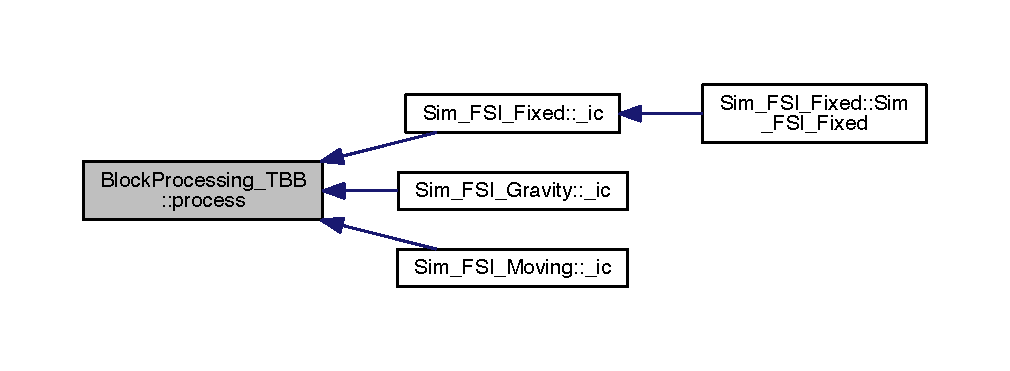
\includegraphics[width=350pt]{d0/d8d/class_block_processing___t_b_b_afb4ac5aee8af3d4e9f3a0f572bdd0a04_icgraph}
\end{center}
\end{figure}


\hypertarget{class_block_processing___t_b_b_a19d9699a50fba9a15eca0e0e1a7f1efd}{}\index{Block\+Processing\+\_\+\+T\+B\+B@{Block\+Processing\+\_\+\+T\+B\+B}!process@{process}}
\index{process@{process}!Block\+Processing\+\_\+\+T\+B\+B@{Block\+Processing\+\_\+\+T\+B\+B}}
\subsubsection[{process}]{\setlength{\rightskip}{0pt plus 5cm}template$<$typename Block\+Type $>$ template$<$typename Lab , typename Grid , typename Processing $>$ static void {\bf Block\+Processing\+\_\+\+T\+B\+B}$<$ Block\+Type $>$\+::process (
\begin{DoxyParamCaption}
\item[{vector$<$ {\bf Block\+Info} $>$ \&}]{v\+Info, }
\item[{Processing \&}]{p, }
\item[{{\bf Grid} \&}]{grid, }
\item[{const {\bf Real}}]{t = {\ttfamily 0}, }
\item[{const bool}]{tensorial = {\ttfamily false}, }
\item[{int}]{n\+Granularity = {\ttfamily -\/1}}
\end{DoxyParamCaption}
)\hspace{0.3cm}{\ttfamily [inline]}, {\ttfamily [static]}}\label{class_block_processing___t_b_b_a19d9699a50fba9a15eca0e0e1a7f1efd}
Process blocks in parallel using parallel\+\_\+for (see tbb-\/doc) to split up the work. 
\begin{DoxyParams}{Parameters}
{\em v\+Info} & Info of all the blocks (to be processed) in the grid (e.\+g. result of \hyperlink{class_grid_a39aa8cb7fad1abcfe40fdd77d9b72d8a}{Grid\+::get\+Blocks\+Info()}). \\
\hline
{\em c} & Collection of all the blocks (to be processed) in the grid (e.\+g. result of Grid\+::get\+Block\+Collection()). \\
\hline
{\em b} & Info on the boundaries of the grid (e.\+g. result of Grid\+::get\+Boundary\+Info()) \\
\hline
{\em p} & Functor processing the block. See M\+R\+A\+G\+::\+Multithreading\+::\+Dummy\+Block\+Functor for details. \\
\hline
{\em n\+Granularity} & Granularity for the parallel\+\_\+for (see tbb-\/doc). Optional\+: if not set, auto\+\_\+partitioner (see tbb-\/doc) will be used. \\
\hline
\end{DoxyParams}


The documentation for this class was generated from the following file\+:\begin{DoxyCompactItemize}
\item 
Cubism/\hyperlink{_block_processing_8h}{Block\+Processing.\+h}\end{DoxyCompactItemize}

\hypertarget{class_block_processing_m_p_i}{}\section{Block\+Processing\+M\+P\+I Class Reference}
\label{class_block_processing_m_p_i}\index{Block\+Processing\+M\+P\+I@{Block\+Processing\+M\+P\+I}}


{\ttfamily \#include $<$Block\+Processing\+M\+P\+I.\+h$>$}

\subsection*{Static Public Member Functions}
\begin{DoxyCompactItemize}
\item 
{\footnotesize template$<$typename Processing , typename Grid $>$ }\\static void \hyperlink{class_block_processing_m_p_i_afdddfef263bdd3f2e5519b701b5299be}{process} (vector$<$ \hyperlink{struct_block_info}{Block\+Info} $>$ \&v\+Info, Processing \&p, \hyperlink{class_grid}{Grid} \&grid, int n\+Granularity=-\/1)
\item 
{\footnotesize template$<$typename Lab , typename Grid , typename Processing $>$ }\\static void \hyperlink{class_block_processing_m_p_i_ad22d78cc5cc53d5e4c05e33ca5ca9c0d}{process} (const vector$<$ \hyperlink{struct_block_info}{Block\+Info} $>$ \&v\+Info, Processing \&p, \hyperlink{class_grid}{Grid} \&grid, const \hyperlink{_h_d_f5_dumper_8h_a445a5f0e2a34c9d97d69a3c2d1957907}{Real} t=0)
\item 
{\footnotesize template$<$typename Lab , typename Grid , typename Processing $>$ }\\static void \hyperlink{class_block_processing_m_p_i_a8b5997288907f3237a965ee7428b8001}{process} (const vector$<$ \hyperlink{struct_block_info}{Block\+Info} $>$ \&v\+Info, Processing \&p, \hyperlink{class_grid}{Grid} \&grid, const \hyperlink{_h_d_f5_dumper_8h_a445a5f0e2a34c9d97d69a3c2d1957907}{Real} t, affinity\+\_\+partitioner \&affinitypart)
\end{DoxyCompactItemize}


\subsection{Member Function Documentation}
\hypertarget{class_block_processing_m_p_i_afdddfef263bdd3f2e5519b701b5299be}{}\index{Block\+Processing\+M\+P\+I@{Block\+Processing\+M\+P\+I}!process@{process}}
\index{process@{process}!Block\+Processing\+M\+P\+I@{Block\+Processing\+M\+P\+I}}
\subsubsection[{process}]{\setlength{\rightskip}{0pt plus 5cm}template$<$typename Processing , typename Grid $>$ static void Block\+Processing\+M\+P\+I\+::process (
\begin{DoxyParamCaption}
\item[{vector$<$ {\bf Block\+Info} $>$ \&}]{v\+Info, }
\item[{Processing \&}]{p, }
\item[{{\bf Grid} \&}]{grid, }
\item[{int}]{n\+Granularity = {\ttfamily -\/1}}
\end{DoxyParamCaption}
)\hspace{0.3cm}{\ttfamily [inline]}, {\ttfamily [static]}}\label{class_block_processing_m_p_i_afdddfef263bdd3f2e5519b701b5299be}
\hypertarget{class_block_processing_m_p_i_ad22d78cc5cc53d5e4c05e33ca5ca9c0d}{}\index{Block\+Processing\+M\+P\+I@{Block\+Processing\+M\+P\+I}!process@{process}}
\index{process@{process}!Block\+Processing\+M\+P\+I@{Block\+Processing\+M\+P\+I}}
\subsubsection[{process}]{\setlength{\rightskip}{0pt plus 5cm}template$<$typename Lab , typename Grid , typename Processing $>$ static void Block\+Processing\+M\+P\+I\+::process (
\begin{DoxyParamCaption}
\item[{const vector$<$ {\bf Block\+Info} $>$ \&}]{v\+Info, }
\item[{Processing \&}]{p, }
\item[{{\bf Grid} \&}]{grid, }
\item[{const {\bf Real}}]{t = {\ttfamily 0}}
\end{DoxyParamCaption}
)\hspace{0.3cm}{\ttfamily [inline]}, {\ttfamily [static]}}\label{class_block_processing_m_p_i_ad22d78cc5cc53d5e4c05e33ca5ca9c0d}
\hypertarget{class_block_processing_m_p_i_a8b5997288907f3237a965ee7428b8001}{}\index{Block\+Processing\+M\+P\+I@{Block\+Processing\+M\+P\+I}!process@{process}}
\index{process@{process}!Block\+Processing\+M\+P\+I@{Block\+Processing\+M\+P\+I}}
\subsubsection[{process}]{\setlength{\rightskip}{0pt plus 5cm}template$<$typename Lab , typename Grid , typename Processing $>$ static void Block\+Processing\+M\+P\+I\+::process (
\begin{DoxyParamCaption}
\item[{const vector$<$ {\bf Block\+Info} $>$ \&}]{v\+Info, }
\item[{Processing \&}]{p, }
\item[{{\bf Grid} \&}]{grid, }
\item[{const {\bf Real}}]{t, }
\item[{affinity\+\_\+partitioner \&}]{affinitypart}
\end{DoxyParamCaption}
)\hspace{0.3cm}{\ttfamily [inline]}, {\ttfamily [static]}}\label{class_block_processing_m_p_i_a8b5997288907f3237a965ee7428b8001}


The documentation for this class was generated from the following file\+:\begin{DoxyCompactItemize}
\item 
/\+Users/cconti/\+Desktop/\+Mounts/\+Brutus\+Home/\+Seed/\+Cubism\+U\+P\+\_\+2\+D/\+Cubism/\hyperlink{_block_processing_m_p_i_8h}{Block\+Processing\+M\+P\+I.\+h}\end{DoxyCompactItemize}

\hypertarget{class_block_processing_m_t___simple___t_b_b}{}\section{Block\+Processing\+M\+T\+\_\+\+Simple\+\_\+\+T\+B\+B$<$ Block\+Type, Processing\+M\+T $>$ Class Template Reference}
\label{class_block_processing_m_t___simple___t_b_b}\index{Block\+Processing\+M\+T\+\_\+\+Simple\+\_\+\+T\+B\+B$<$ Block\+Type, Processing\+M\+T $>$@{Block\+Processing\+M\+T\+\_\+\+Simple\+\_\+\+T\+B\+B$<$ Block\+Type, Processing\+M\+T $>$}}


{\ttfamily \#include $<$Block\+Processing.\+h$>$}

\subsection*{Public Member Functions}
\begin{DoxyCompactItemize}
\item 
\hyperlink{class_block_processing_m_t___simple___t_b_b_a691756211b9c0a9569522ebcb450027a}{Block\+Processing\+M\+T\+\_\+\+Simple\+\_\+\+T\+B\+B} (const \hyperlink{struct_block_info}{Block\+Info} $\ast$ptr\+Infos\+\_\+, Processing\+M\+T \&processing\+\_\+)
\item 
\hyperlink{class_block_processing_m_t___simple___t_b_b_ae61c509d7c1e21ab320ebd8662240aa3}{Block\+Processing\+M\+T\+\_\+\+Simple\+\_\+\+T\+B\+B} (const \hyperlink{class_block_processing_m_t___simple___t_b_b}{Block\+Processing\+M\+T\+\_\+\+Simple\+\_\+\+T\+B\+B} \&p)
\item 
\hyperlink{class_block_processing_m_t___simple___t_b_b}{Block\+Processing\+M\+T\+\_\+\+Simple\+\_\+\+T\+B\+B} \& \hyperlink{class_block_processing_m_t___simple___t_b_b_ac5597c90925243796b290b21269e9e63}{operator=} (const \hyperlink{class_block_processing_m_t___simple___t_b_b}{Block\+Processing\+M\+T\+\_\+\+Simple\+\_\+\+T\+B\+B} \&p)
\item 
{\footnotesize template$<$typename Blocked\+Range $>$ }\\void \hyperlink{class_block_processing_m_t___simple___t_b_b_a57abb7f3b784cca155c948b93b04b570}{operator()} (const Blocked\+Range \&r) const 
\end{DoxyCompactItemize}


\subsection{Detailed Description}
\subsubsection*{template$<$typename Block\+Type, typename Processing\+M\+T$>$class Block\+Processing\+M\+T\+\_\+\+Simple\+\_\+\+T\+B\+B$<$ Block\+Type, Processing\+M\+T $>$}

Functor to actually perform the operations on the blocks. 

\subsection{Constructor \& Destructor Documentation}
\hypertarget{class_block_processing_m_t___simple___t_b_b_a691756211b9c0a9569522ebcb450027a}{}\index{Block\+Processing\+M\+T\+\_\+\+Simple\+\_\+\+T\+B\+B@{Block\+Processing\+M\+T\+\_\+\+Simple\+\_\+\+T\+B\+B}!Block\+Processing\+M\+T\+\_\+\+Simple\+\_\+\+T\+B\+B@{Block\+Processing\+M\+T\+\_\+\+Simple\+\_\+\+T\+B\+B}}
\index{Block\+Processing\+M\+T\+\_\+\+Simple\+\_\+\+T\+B\+B@{Block\+Processing\+M\+T\+\_\+\+Simple\+\_\+\+T\+B\+B}!Block\+Processing\+M\+T\+\_\+\+Simple\+\_\+\+T\+B\+B@{Block\+Processing\+M\+T\+\_\+\+Simple\+\_\+\+T\+B\+B}}
\subsubsection[{Block\+Processing\+M\+T\+\_\+\+Simple\+\_\+\+T\+B\+B}]{\setlength{\rightskip}{0pt plus 5cm}template$<$typename Block\+Type, typename Processing\+M\+T$>$ {\bf Block\+Processing\+M\+T\+\_\+\+Simple\+\_\+\+T\+B\+B}$<$ Block\+Type, Processing\+M\+T $>$\+::{\bf Block\+Processing\+M\+T\+\_\+\+Simple\+\_\+\+T\+B\+B} (
\begin{DoxyParamCaption}
\item[{const {\bf Block\+Info} $\ast$}]{ptr\+Infos\+\_\+, }
\item[{Processing\+M\+T \&}]{processing\+\_\+}
\end{DoxyParamCaption}
)\hspace{0.3cm}{\ttfamily [inline]}}\label{class_block_processing_m_t___simple___t_b_b_a691756211b9c0a9569522ebcb450027a}
\hypertarget{class_block_processing_m_t___simple___t_b_b_ae61c509d7c1e21ab320ebd8662240aa3}{}\index{Block\+Processing\+M\+T\+\_\+\+Simple\+\_\+\+T\+B\+B@{Block\+Processing\+M\+T\+\_\+\+Simple\+\_\+\+T\+B\+B}!Block\+Processing\+M\+T\+\_\+\+Simple\+\_\+\+T\+B\+B@{Block\+Processing\+M\+T\+\_\+\+Simple\+\_\+\+T\+B\+B}}
\index{Block\+Processing\+M\+T\+\_\+\+Simple\+\_\+\+T\+B\+B@{Block\+Processing\+M\+T\+\_\+\+Simple\+\_\+\+T\+B\+B}!Block\+Processing\+M\+T\+\_\+\+Simple\+\_\+\+T\+B\+B@{Block\+Processing\+M\+T\+\_\+\+Simple\+\_\+\+T\+B\+B}}
\subsubsection[{Block\+Processing\+M\+T\+\_\+\+Simple\+\_\+\+T\+B\+B}]{\setlength{\rightskip}{0pt plus 5cm}template$<$typename Block\+Type, typename Processing\+M\+T$>$ {\bf Block\+Processing\+M\+T\+\_\+\+Simple\+\_\+\+T\+B\+B}$<$ Block\+Type, Processing\+M\+T $>$\+::{\bf Block\+Processing\+M\+T\+\_\+\+Simple\+\_\+\+T\+B\+B} (
\begin{DoxyParamCaption}
\item[{const {\bf Block\+Processing\+M\+T\+\_\+\+Simple\+\_\+\+T\+B\+B}$<$ Block\+Type, Processing\+M\+T $>$ \&}]{p}
\end{DoxyParamCaption}
)\hspace{0.3cm}{\ttfamily [inline]}}\label{class_block_processing_m_t___simple___t_b_b_ae61c509d7c1e21ab320ebd8662240aa3}


\subsection{Member Function Documentation}
\hypertarget{class_block_processing_m_t___simple___t_b_b_a57abb7f3b784cca155c948b93b04b570}{}\index{Block\+Processing\+M\+T\+\_\+\+Simple\+\_\+\+T\+B\+B@{Block\+Processing\+M\+T\+\_\+\+Simple\+\_\+\+T\+B\+B}!operator()@{operator()}}
\index{operator()@{operator()}!Block\+Processing\+M\+T\+\_\+\+Simple\+\_\+\+T\+B\+B@{Block\+Processing\+M\+T\+\_\+\+Simple\+\_\+\+T\+B\+B}}
\subsubsection[{operator()}]{\setlength{\rightskip}{0pt plus 5cm}template$<$typename Block\+Type, typename Processing\+M\+T$>$ template$<$typename Blocked\+Range $>$ void {\bf Block\+Processing\+M\+T\+\_\+\+Simple\+\_\+\+T\+B\+B}$<$ Block\+Type, Processing\+M\+T $>$\+::operator() (
\begin{DoxyParamCaption}
\item[{const Blocked\+Range \&}]{r}
\end{DoxyParamCaption}
) const\hspace{0.3cm}{\ttfamily [inline]}}\label{class_block_processing_m_t___simple___t_b_b_a57abb7f3b784cca155c948b93b04b570}
\hypertarget{class_block_processing_m_t___simple___t_b_b_ac5597c90925243796b290b21269e9e63}{}\index{Block\+Processing\+M\+T\+\_\+\+Simple\+\_\+\+T\+B\+B@{Block\+Processing\+M\+T\+\_\+\+Simple\+\_\+\+T\+B\+B}!operator=@{operator=}}
\index{operator=@{operator=}!Block\+Processing\+M\+T\+\_\+\+Simple\+\_\+\+T\+B\+B@{Block\+Processing\+M\+T\+\_\+\+Simple\+\_\+\+T\+B\+B}}
\subsubsection[{operator=}]{\setlength{\rightskip}{0pt plus 5cm}template$<$typename Block\+Type, typename Processing\+M\+T$>$ {\bf Block\+Processing\+M\+T\+\_\+\+Simple\+\_\+\+T\+B\+B}\& {\bf Block\+Processing\+M\+T\+\_\+\+Simple\+\_\+\+T\+B\+B}$<$ Block\+Type, Processing\+M\+T $>$\+::operator= (
\begin{DoxyParamCaption}
\item[{const {\bf Block\+Processing\+M\+T\+\_\+\+Simple\+\_\+\+T\+B\+B}$<$ Block\+Type, Processing\+M\+T $>$ \&}]{p}
\end{DoxyParamCaption}
)\hspace{0.3cm}{\ttfamily [inline]}}\label{class_block_processing_m_t___simple___t_b_b_ac5597c90925243796b290b21269e9e63}


The documentation for this class was generated from the following file\+:\begin{DoxyCompactItemize}
\item 
/\+Users/cconti/\+Desktop/\+Mounts/\+Brutus\+Home/\+Seed/\+Cubism\+U\+P\+\_\+2\+D/\+Cubism/\hyperlink{_block_processing_8h}{Block\+Processing.\+h}\end{DoxyCompactItemize}

\hypertarget{class_block_processing_m_t___t_b_b}{}\section{Block\+Processing\+M\+T\+\_\+\+T\+B\+B$<$ Grid, Lab, Processing\+M\+T, n\+Slots $>$ Class Template Reference}
\label{class_block_processing_m_t___t_b_b}\index{Block\+Processing\+M\+T\+\_\+\+T\+B\+B$<$ Grid, Lab, Processing\+M\+T, n\+Slots $>$@{Block\+Processing\+M\+T\+\_\+\+T\+B\+B$<$ Grid, Lab, Processing\+M\+T, n\+Slots $>$}}


{\ttfamily \#include $<$Block\+Processing.\+h$>$}

\subsection*{Public Member Functions}
\begin{DoxyCompactItemize}
\item 
\hyperlink{class_block_processing_m_t___t_b_b_ab593a07d303a80c94ad90df501d82dad}{Block\+Processing\+M\+T\+\_\+\+T\+B\+B} (concurrent\+\_\+queue$<$ \hyperlink{_definitions_8h_ad6f951af9a2a6ebc1975404882b34314}{Lab} $\ast$ $>$ \&available\+Labs, const \hyperlink{struct_block_info}{Block\+Info} $\ast$ptr\+Infos\+\_\+, \hyperlink{class_grid}{Grid} \&grid, Processing\+M\+T \&processing\+\_\+, const \hyperlink{_h_d_f5_dumper_8h_a445a5f0e2a34c9d97d69a3c2d1957907}{Real} t=0, const bool tensorial=false)
\item 
{\footnotesize template$<$typename Blocked\+Range $>$ }\\void \hyperlink{class_block_processing_m_t___t_b_b_aaef2110d9801cdcb5aec76b1d0c1e343}{operator()} (const Blocked\+Range \&r) const 
\item 
\hyperlink{class_block_processing_m_t___t_b_b_acf41642fa9233a7557a098285e5dd60c}{Block\+Processing\+M\+T\+\_\+\+T\+B\+B} (const \hyperlink{class_block_processing_m_t___t_b_b}{Block\+Processing\+M\+T\+\_\+\+T\+B\+B} \&p)
\end{DoxyCompactItemize}


\subsection{Constructor \& Destructor Documentation}
\hypertarget{class_block_processing_m_t___t_b_b_ab593a07d303a80c94ad90df501d82dad}{}\index{Block\+Processing\+M\+T\+\_\+\+T\+B\+B@{Block\+Processing\+M\+T\+\_\+\+T\+B\+B}!Block\+Processing\+M\+T\+\_\+\+T\+B\+B@{Block\+Processing\+M\+T\+\_\+\+T\+B\+B}}
\index{Block\+Processing\+M\+T\+\_\+\+T\+B\+B@{Block\+Processing\+M\+T\+\_\+\+T\+B\+B}!Block\+Processing\+M\+T\+\_\+\+T\+B\+B@{Block\+Processing\+M\+T\+\_\+\+T\+B\+B}}
\subsubsection[{Block\+Processing\+M\+T\+\_\+\+T\+B\+B}]{\setlength{\rightskip}{0pt plus 5cm}template$<$typename Grid, typename Lab, typename Processing\+M\+T, int n\+Slots$>$ {\bf Block\+Processing\+M\+T\+\_\+\+T\+B\+B}$<$ {\bf Grid}, {\bf Lab}, Processing\+M\+T, n\+Slots $>$\+::{\bf Block\+Processing\+M\+T\+\_\+\+T\+B\+B} (
\begin{DoxyParamCaption}
\item[{concurrent\+\_\+queue$<$ {\bf Lab} $\ast$ $>$ \&}]{available\+Labs, }
\item[{const {\bf Block\+Info} $\ast$}]{ptr\+Infos\+\_\+, }
\item[{{\bf Grid} \&}]{grid, }
\item[{Processing\+M\+T \&}]{processing\+\_\+, }
\item[{const {\bf Real}}]{t = {\ttfamily 0}, }
\item[{const bool}]{tensorial = {\ttfamily false}}
\end{DoxyParamCaption}
)\hspace{0.3cm}{\ttfamily [inline]}}\label{class_block_processing_m_t___t_b_b_ab593a07d303a80c94ad90df501d82dad}


Here is the call graph for this function\+:
% FIG 0


\hypertarget{class_block_processing_m_t___t_b_b_acf41642fa9233a7557a098285e5dd60c}{}\index{Block\+Processing\+M\+T\+\_\+\+T\+B\+B@{Block\+Processing\+M\+T\+\_\+\+T\+B\+B}!Block\+Processing\+M\+T\+\_\+\+T\+B\+B@{Block\+Processing\+M\+T\+\_\+\+T\+B\+B}}
\index{Block\+Processing\+M\+T\+\_\+\+T\+B\+B@{Block\+Processing\+M\+T\+\_\+\+T\+B\+B}!Block\+Processing\+M\+T\+\_\+\+T\+B\+B@{Block\+Processing\+M\+T\+\_\+\+T\+B\+B}}
\subsubsection[{Block\+Processing\+M\+T\+\_\+\+T\+B\+B}]{\setlength{\rightskip}{0pt plus 5cm}template$<$typename Grid, typename Lab, typename Processing\+M\+T, int n\+Slots$>$ {\bf Block\+Processing\+M\+T\+\_\+\+T\+B\+B}$<$ {\bf Grid}, {\bf Lab}, Processing\+M\+T, n\+Slots $>$\+::{\bf Block\+Processing\+M\+T\+\_\+\+T\+B\+B} (
\begin{DoxyParamCaption}
\item[{const {\bf Block\+Processing\+M\+T\+\_\+\+T\+B\+B}$<$ {\bf Grid}, {\bf Lab}, Processing\+M\+T, n\+Slots $>$ \&}]{p}
\end{DoxyParamCaption}
)\hspace{0.3cm}{\ttfamily [inline]}}\label{class_block_processing_m_t___t_b_b_acf41642fa9233a7557a098285e5dd60c}


\subsection{Member Function Documentation}
\hypertarget{class_block_processing_m_t___t_b_b_aaef2110d9801cdcb5aec76b1d0c1e343}{}\index{Block\+Processing\+M\+T\+\_\+\+T\+B\+B@{Block\+Processing\+M\+T\+\_\+\+T\+B\+B}!operator()@{operator()}}
\index{operator()@{operator()}!Block\+Processing\+M\+T\+\_\+\+T\+B\+B@{Block\+Processing\+M\+T\+\_\+\+T\+B\+B}}
\subsubsection[{operator()}]{\setlength{\rightskip}{0pt plus 5cm}template$<$typename Grid, typename Lab, typename Processing\+M\+T, int n\+Slots$>$ template$<$typename Blocked\+Range $>$ void {\bf Block\+Processing\+M\+T\+\_\+\+T\+B\+B}$<$ {\bf Grid}, {\bf Lab}, Processing\+M\+T, n\+Slots $>$\+::operator() (
\begin{DoxyParamCaption}
\item[{const Blocked\+Range \&}]{r}
\end{DoxyParamCaption}
) const\hspace{0.3cm}{\ttfamily [inline]}}\label{class_block_processing_m_t___t_b_b_aaef2110d9801cdcb5aec76b1d0c1e343}


Here is the call graph for this function\+:
% FIG 1




The documentation for this class was generated from the following file\+:\begin{DoxyCompactItemize}
\item 
/\+Users/cconti/\+Desktop/\+Mounts/\+Brutus\+Home/\+Seed/\+Cubism\+U\+P\+\_\+2\+D/\+Cubism/\hyperlink{_block_processing_8h}{Block\+Processing.\+h}\end{DoxyCompactItemize}

\hypertarget{class_boundary_condition}{}\section{Boundary\+Condition$<$ T\+Block, T\+Element, allocator $>$ Class Template Reference}
\label{class_boundary_condition}\index{Boundary\+Condition$<$ T\+Block, T\+Element, allocator $>$@{Boundary\+Condition$<$ T\+Block, T\+Element, allocator $>$}}


{\ttfamily \#include $<$Boundary\+Conditions.\+h$>$}



Collaboration diagram for Boundary\+Condition$<$ T\+Block, T\+Element, allocator $>$\+:\nopagebreak
\begin{figure}[H]
\begin{center}
\leavevmode
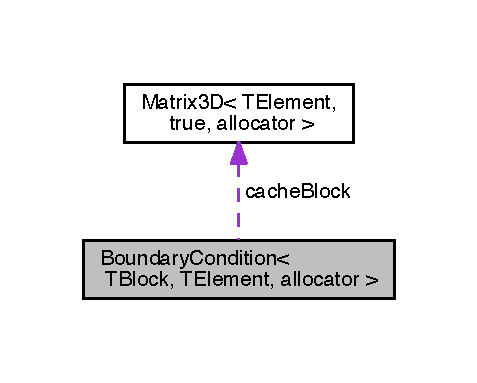
\includegraphics[width=229pt]{d7/d21/class_boundary_condition__coll__graph}
\end{center}
\end{figure}
\subsection*{Public Member Functions}
\begin{DoxyCompactItemize}
\item 
\hyperlink{class_boundary_condition_a89cbd322bff8127af5a49685e3bf04ce}{Boundary\+Condition} (const int ss\mbox{[}3\mbox{]}, const int se\mbox{[}3\mbox{]}, \hyperlink{class_matrix3_d}{Matrix3\+D}$<$ T\+Element, true, allocator $>$ $\ast$\hyperlink{class_boundary_condition_a1e0c33fa794a6d333d4451f8fde04c29}{cache\+Block})
\item 
T\+Element \& \hyperlink{class_boundary_condition_aadcfe05da7761b68191835b09d4d2cf0}{operator()} (int ix, int iy)
\item 
{\footnotesize template$<$int dir, int side$>$ }\\void \hyperlink{class_boundary_condition_adadad3f69ee5cf8ab11dc8f8a7763a4f}{apply\+B\+C\+\_\+dirichlet} (const T\+Element \&p)
\item 
{\footnotesize template$<$int dir, int side$>$ }\\void \hyperlink{class_boundary_condition_a101992951fb756135ca3e44f5d64bb60}{apply\+B\+C\+\_\+neumann} ()
\item 
{\footnotesize template$<$int dir, int side$>$ }\\void \hyperlink{class_boundary_condition_a60e154d33104f42e29dfa49061b266f6}{apply\+B\+C\+\_\+mixed\+Bottom} ()
\item 
{\footnotesize template$<$int dir, int side$>$ }\\void \hyperlink{class_boundary_condition_a77cf65bd542d198d80aa54a3de632ff5}{apply\+B\+C\+\_\+mixed\+Top} ()
\end{DoxyCompactItemize}
\subsection*{Protected Member Functions}
\begin{DoxyCompactItemize}
\item 
{\footnotesize template$<$int dir, int side$>$ }\\void \hyperlink{class_boundary_condition_af8969c6c584388f44cf464a8021d125a}{\+\_\+setup} ()
\end{DoxyCompactItemize}
\subsection*{Protected Attributes}
\begin{DoxyCompactItemize}
\item 
int \hyperlink{class_boundary_condition_a7734cfc6ee1ce3a1dea426ab289a299a}{s} \mbox{[}3\mbox{]}
\item 
int \hyperlink{class_boundary_condition_a755da05bbc5a09adb17a6f1e5a15f25b}{e} \mbox{[}3\mbox{]}
\item 
int \hyperlink{class_boundary_condition_aed1e3cfd20d69c6084d901c246698fdd}{stencil\+Start} \mbox{[}3\mbox{]}
\item 
int \hyperlink{class_boundary_condition_af396b479ba0487ba5c0e45d5b636f09e}{stencil\+End} \mbox{[}3\mbox{]}
\item 
\hyperlink{class_matrix3_d}{Matrix3\+D}$<$ T\+Element, true, allocator $>$ $\ast$ \hyperlink{class_boundary_condition_a1e0c33fa794a6d333d4451f8fde04c29}{cache\+Block}
\end{DoxyCompactItemize}


\subsection{Constructor \& Destructor Documentation}
\hypertarget{class_boundary_condition_a89cbd322bff8127af5a49685e3bf04ce}{}\index{Boundary\+Condition@{Boundary\+Condition}!Boundary\+Condition@{Boundary\+Condition}}
\index{Boundary\+Condition@{Boundary\+Condition}!Boundary\+Condition@{Boundary\+Condition}}
\subsubsection[{Boundary\+Condition}]{\setlength{\rightskip}{0pt plus 5cm}template$<$typename T\+Block, typename T\+Element, template$<$ typename X $>$ class allocator = std\+::allocator$>$ {\bf Boundary\+Condition}$<$ T\+Block, T\+Element, allocator $>$\+::{\bf Boundary\+Condition} (
\begin{DoxyParamCaption}
\item[{const int}]{ss\mbox{[}3\mbox{]}, }
\item[{const int}]{se\mbox{[}3\mbox{]}, }
\item[{{\bf Matrix3\+D}$<$ T\+Element, true, allocator $>$ $\ast$}]{cache\+Block}
\end{DoxyParamCaption}
)\hspace{0.3cm}{\ttfamily [inline]}}\label{class_boundary_condition_a89cbd322bff8127af5a49685e3bf04ce}


\subsection{Member Function Documentation}
\hypertarget{class_boundary_condition_af8969c6c584388f44cf464a8021d125a}{}\index{Boundary\+Condition@{Boundary\+Condition}!\+\_\+setup@{\+\_\+setup}}
\index{\+\_\+setup@{\+\_\+setup}!Boundary\+Condition@{Boundary\+Condition}}
\subsubsection[{\+\_\+setup}]{\setlength{\rightskip}{0pt plus 5cm}template$<$typename T\+Block, typename T\+Element, template$<$ typename X $>$ class allocator = std\+::allocator$>$ template$<$int dir, int side$>$ void {\bf Boundary\+Condition}$<$ T\+Block, T\+Element, allocator $>$\+::\+\_\+setup (
\begin{DoxyParamCaption}
{}
\end{DoxyParamCaption}
)\hspace{0.3cm}{\ttfamily [inline]}, {\ttfamily [protected]}}\label{class_boundary_condition_af8969c6c584388f44cf464a8021d125a}
\hypertarget{class_boundary_condition_adadad3f69ee5cf8ab11dc8f8a7763a4f}{}\index{Boundary\+Condition@{Boundary\+Condition}!apply\+B\+C\+\_\+dirichlet@{apply\+B\+C\+\_\+dirichlet}}
\index{apply\+B\+C\+\_\+dirichlet@{apply\+B\+C\+\_\+dirichlet}!Boundary\+Condition@{Boundary\+Condition}}
\subsubsection[{apply\+B\+C\+\_\+dirichlet}]{\setlength{\rightskip}{0pt plus 5cm}template$<$typename T\+Block, typename T\+Element, template$<$ typename X $>$ class allocator = std\+::allocator$>$ template$<$int dir, int side$>$ void {\bf Boundary\+Condition}$<$ T\+Block, T\+Element, allocator $>$\+::apply\+B\+C\+\_\+dirichlet (
\begin{DoxyParamCaption}
\item[{const T\+Element \&}]{p}
\end{DoxyParamCaption}
)\hspace{0.3cm}{\ttfamily [inline]}}\label{class_boundary_condition_adadad3f69ee5cf8ab11dc8f8a7763a4f}
\hypertarget{class_boundary_condition_a60e154d33104f42e29dfa49061b266f6}{}\index{Boundary\+Condition@{Boundary\+Condition}!apply\+B\+C\+\_\+mixed\+Bottom@{apply\+B\+C\+\_\+mixed\+Bottom}}
\index{apply\+B\+C\+\_\+mixed\+Bottom@{apply\+B\+C\+\_\+mixed\+Bottom}!Boundary\+Condition@{Boundary\+Condition}}
\subsubsection[{apply\+B\+C\+\_\+mixed\+Bottom}]{\setlength{\rightskip}{0pt plus 5cm}template$<$typename T\+Block, typename T\+Element, template$<$ typename X $>$ class allocator = std\+::allocator$>$ template$<$int dir, int side$>$ void {\bf Boundary\+Condition}$<$ T\+Block, T\+Element, allocator $>$\+::apply\+B\+C\+\_\+mixed\+Bottom (
\begin{DoxyParamCaption}
{}
\end{DoxyParamCaption}
)\hspace{0.3cm}{\ttfamily [inline]}}\label{class_boundary_condition_a60e154d33104f42e29dfa49061b266f6}
\hypertarget{class_boundary_condition_a77cf65bd542d198d80aa54a3de632ff5}{}\index{Boundary\+Condition@{Boundary\+Condition}!apply\+B\+C\+\_\+mixed\+Top@{apply\+B\+C\+\_\+mixed\+Top}}
\index{apply\+B\+C\+\_\+mixed\+Top@{apply\+B\+C\+\_\+mixed\+Top}!Boundary\+Condition@{Boundary\+Condition}}
\subsubsection[{apply\+B\+C\+\_\+mixed\+Top}]{\setlength{\rightskip}{0pt plus 5cm}template$<$typename T\+Block, typename T\+Element, template$<$ typename X $>$ class allocator = std\+::allocator$>$ template$<$int dir, int side$>$ void {\bf Boundary\+Condition}$<$ T\+Block, T\+Element, allocator $>$\+::apply\+B\+C\+\_\+mixed\+Top (
\begin{DoxyParamCaption}
{}
\end{DoxyParamCaption}
)\hspace{0.3cm}{\ttfamily [inline]}}\label{class_boundary_condition_a77cf65bd542d198d80aa54a3de632ff5}
\hypertarget{class_boundary_condition_a101992951fb756135ca3e44f5d64bb60}{}\index{Boundary\+Condition@{Boundary\+Condition}!apply\+B\+C\+\_\+neumann@{apply\+B\+C\+\_\+neumann}}
\index{apply\+B\+C\+\_\+neumann@{apply\+B\+C\+\_\+neumann}!Boundary\+Condition@{Boundary\+Condition}}
\subsubsection[{apply\+B\+C\+\_\+neumann}]{\setlength{\rightskip}{0pt plus 5cm}template$<$typename T\+Block, typename T\+Element, template$<$ typename X $>$ class allocator = std\+::allocator$>$ template$<$int dir, int side$>$ void {\bf Boundary\+Condition}$<$ T\+Block, T\+Element, allocator $>$\+::apply\+B\+C\+\_\+neumann (
\begin{DoxyParamCaption}
{}
\end{DoxyParamCaption}
)\hspace{0.3cm}{\ttfamily [inline]}}\label{class_boundary_condition_a101992951fb756135ca3e44f5d64bb60}
\hypertarget{class_boundary_condition_aadcfe05da7761b68191835b09d4d2cf0}{}\index{Boundary\+Condition@{Boundary\+Condition}!operator()@{operator()}}
\index{operator()@{operator()}!Boundary\+Condition@{Boundary\+Condition}}
\subsubsection[{operator()}]{\setlength{\rightskip}{0pt plus 5cm}template$<$typename T\+Block, typename T\+Element, template$<$ typename X $>$ class allocator = std\+::allocator$>$ T\+Element\& {\bf Boundary\+Condition}$<$ T\+Block, T\+Element, allocator $>$\+::operator() (
\begin{DoxyParamCaption}
\item[{int}]{ix, }
\item[{int}]{iy}
\end{DoxyParamCaption}
)\hspace{0.3cm}{\ttfamily [inline]}}\label{class_boundary_condition_aadcfe05da7761b68191835b09d4d2cf0}


Here is the call graph for this function\+:\nopagebreak
\begin{figure}[H]
\begin{center}
\leavevmode
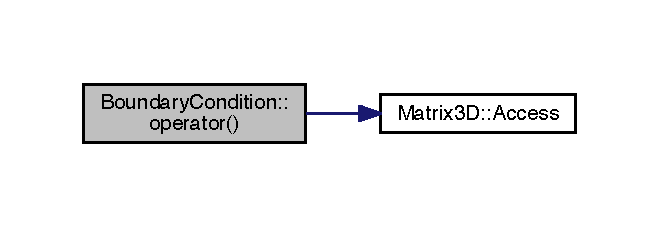
\includegraphics[width=316pt]{db/d64/class_boundary_condition_aadcfe05da7761b68191835b09d4d2cf0_cgraph}
\end{center}
\end{figure}




\subsection{Member Data Documentation}
\hypertarget{class_boundary_condition_a1e0c33fa794a6d333d4451f8fde04c29}{}\index{Boundary\+Condition@{Boundary\+Condition}!cache\+Block@{cache\+Block}}
\index{cache\+Block@{cache\+Block}!Boundary\+Condition@{Boundary\+Condition}}
\subsubsection[{cache\+Block}]{\setlength{\rightskip}{0pt plus 5cm}template$<$typename T\+Block, typename T\+Element, template$<$ typename X $>$ class allocator = std\+::allocator$>$ {\bf Matrix3\+D}$<$T\+Element, true, allocator$>$$\ast$ {\bf Boundary\+Condition}$<$ T\+Block, T\+Element, allocator $>$\+::cache\+Block\hspace{0.3cm}{\ttfamily [protected]}}\label{class_boundary_condition_a1e0c33fa794a6d333d4451f8fde04c29}
\hypertarget{class_boundary_condition_a755da05bbc5a09adb17a6f1e5a15f25b}{}\index{Boundary\+Condition@{Boundary\+Condition}!e@{e}}
\index{e@{e}!Boundary\+Condition@{Boundary\+Condition}}
\subsubsection[{e}]{\setlength{\rightskip}{0pt plus 5cm}template$<$typename T\+Block, typename T\+Element, template$<$ typename X $>$ class allocator = std\+::allocator$>$ int {\bf Boundary\+Condition}$<$ T\+Block, T\+Element, allocator $>$\+::e\mbox{[}3\mbox{]}\hspace{0.3cm}{\ttfamily [protected]}}\label{class_boundary_condition_a755da05bbc5a09adb17a6f1e5a15f25b}
\hypertarget{class_boundary_condition_a7734cfc6ee1ce3a1dea426ab289a299a}{}\index{Boundary\+Condition@{Boundary\+Condition}!s@{s}}
\index{s@{s}!Boundary\+Condition@{Boundary\+Condition}}
\subsubsection[{s}]{\setlength{\rightskip}{0pt plus 5cm}template$<$typename T\+Block, typename T\+Element, template$<$ typename X $>$ class allocator = std\+::allocator$>$ int {\bf Boundary\+Condition}$<$ T\+Block, T\+Element, allocator $>$\+::s\mbox{[}3\mbox{]}\hspace{0.3cm}{\ttfamily [protected]}}\label{class_boundary_condition_a7734cfc6ee1ce3a1dea426ab289a299a}
\hypertarget{class_boundary_condition_af396b479ba0487ba5c0e45d5b636f09e}{}\index{Boundary\+Condition@{Boundary\+Condition}!stencil\+End@{stencil\+End}}
\index{stencil\+End@{stencil\+End}!Boundary\+Condition@{Boundary\+Condition}}
\subsubsection[{stencil\+End}]{\setlength{\rightskip}{0pt plus 5cm}template$<$typename T\+Block, typename T\+Element, template$<$ typename X $>$ class allocator = std\+::allocator$>$ int {\bf Boundary\+Condition}$<$ T\+Block, T\+Element, allocator $>$\+::stencil\+End\mbox{[}3\mbox{]}\hspace{0.3cm}{\ttfamily [protected]}}\label{class_boundary_condition_af396b479ba0487ba5c0e45d5b636f09e}
\hypertarget{class_boundary_condition_aed1e3cfd20d69c6084d901c246698fdd}{}\index{Boundary\+Condition@{Boundary\+Condition}!stencil\+Start@{stencil\+Start}}
\index{stencil\+Start@{stencil\+Start}!Boundary\+Condition@{Boundary\+Condition}}
\subsubsection[{stencil\+Start}]{\setlength{\rightskip}{0pt plus 5cm}template$<$typename T\+Block, typename T\+Element, template$<$ typename X $>$ class allocator = std\+::allocator$>$ int {\bf Boundary\+Condition}$<$ T\+Block, T\+Element, allocator $>$\+::stencil\+Start\mbox{[}3\mbox{]}\hspace{0.3cm}{\ttfamily [protected]}}\label{class_boundary_condition_aed1e3cfd20d69c6084d901c246698fdd}


The documentation for this class was generated from the following file\+:\begin{DoxyCompactItemize}
\item 
source/\hyperlink{_boundary_conditions_8h}{Boundary\+Conditions.\+h}\end{DoxyCompactItemize}

\hypertarget{class_b_s4}{}\section{B\+S4 Class Reference}
\label{class_b_s4}\index{B\+S4@{B\+S4}}
\subsection*{Static Public Member Functions}
\begin{DoxyCompactItemize}
\item 
static \hyperlink{_h_d_f5_dumper_8h_a445a5f0e2a34c9d97d69a3c2d1957907}{Real} \hyperlink{class_b_s4_ab53524385d759ff3e1fafa9b53aee574}{eval} (\hyperlink{_h_d_f5_dumper_8h_a445a5f0e2a34c9d97d69a3c2d1957907}{Real} x)
\item 
static \hyperlink{_h_d_f5_dumper_8h_a445a5f0e2a34c9d97d69a3c2d1957907}{Real} \hyperlink{class_b_s4_ab53524385d759ff3e1fafa9b53aee574}{eval} (\hyperlink{_h_d_f5_dumper_8h_a445a5f0e2a34c9d97d69a3c2d1957907}{Real} x)
\end{DoxyCompactItemize}


\subsection{Member Function Documentation}
\hypertarget{class_b_s4_ab53524385d759ff3e1fafa9b53aee574}{}\index{B\+S4@{B\+S4}!eval@{eval}}
\index{eval@{eval}!B\+S4@{B\+S4}}
\subsubsection[{eval}]{\setlength{\rightskip}{0pt plus 5cm}static {\bf Real} B\+S4\+::eval (
\begin{DoxyParamCaption}
\item[{{\bf Real}}]{x}
\end{DoxyParamCaption}
)\hspace{0.3cm}{\ttfamily [inline]}, {\ttfamily [static]}}\label{class_b_s4_ab53524385d759ff3e1fafa9b53aee574}


Here is the caller graph for this function\+:\nopagebreak
\begin{figure}[H]
\begin{center}
\leavevmode
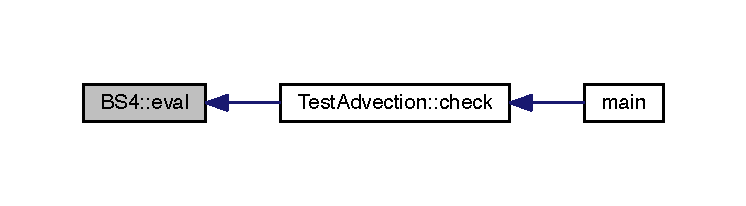
\includegraphics[width=350pt]{d3/d24/class_b_s4_ab53524385d759ff3e1fafa9b53aee574_icgraph}
\end{center}
\end{figure}


\hypertarget{class_b_s4_ab53524385d759ff3e1fafa9b53aee574}{}\index{B\+S4@{B\+S4}!eval@{eval}}
\index{eval@{eval}!B\+S4@{B\+S4}}
\subsubsection[{eval}]{\setlength{\rightskip}{0pt plus 5cm}static {\bf Real} B\+S4\+::eval (
\begin{DoxyParamCaption}
\item[{{\bf Real}}]{x}
\end{DoxyParamCaption}
)\hspace{0.3cm}{\ttfamily [inline]}, {\ttfamily [static]}}\label{class_b_s4_ab53524385d759ff3e1fafa9b53aee574}


The documentation for this class was generated from the following files\+:\begin{DoxyCompactItemize}
\item 
source/\hyperlink{_test_advection_8cpp}{Test\+Advection.\+cpp}\item 
source/\hyperlink{_test_pressure_8cpp}{Test\+Pressure.\+cpp}\end{DoxyCompactItemize}

\hypertarget{struct_dependency_cube_m_p_i_1_1_corner}{}\section{Dependency\+Cube\+M\+P\+I$<$ Request $>$\+:\+:Corner Struct Reference}
\label{struct_dependency_cube_m_p_i_1_1_corner}\index{Dependency\+Cube\+M\+P\+I$<$ Request $>$\+::\+Corner@{Dependency\+Cube\+M\+P\+I$<$ Request $>$\+::\+Corner}}


{\ttfamily \#include $<$Dependency\+Cube\+M\+P\+I.\+h$>$}



Inheritance diagram for Dependency\+Cube\+M\+P\+I$<$ Request $>$\+:\+:Corner\+:\nopagebreak
\begin{figure}[H]
\begin{center}
\leavevmode
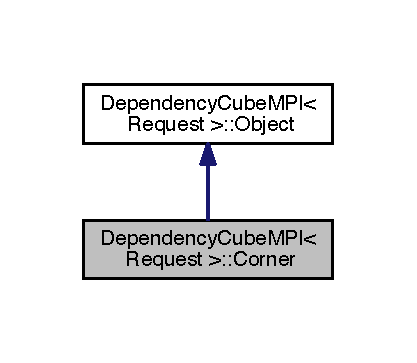
\includegraphics[width=200pt]{db/daf/struct_dependency_cube_m_p_i_1_1_corner__inherit__graph}
\end{center}
\end{figure}


Collaboration diagram for Dependency\+Cube\+M\+P\+I$<$ Request $>$\+:\+:Corner\+:\nopagebreak
\begin{figure}[H]
\begin{center}
\leavevmode
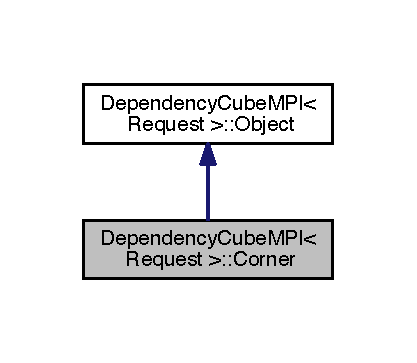
\includegraphics[width=200pt]{d3/df4/struct_dependency_cube_m_p_i_1_1_corner__coll__graph}
\end{center}
\end{figure}
\subsection*{Public Member Functions}
\begin{DoxyCompactItemize}
\item 
\hyperlink{struct_dependency_cube_m_p_i_1_1_corner_aaaca0d2df83a56574746366604e29801}{Corner} ()
\item 
\hyperlink{struct_dependency_cube_m_p_i_1_1_corner_acf350554c41d738d9f8a851e3a798e55}{Corner} (Side \hyperlink{struct_dependency_cube_m_p_i_1_1_corner_a941a0145078d057ead36939decc93c67}{x}, Side \hyperlink{struct_dependency_cube_m_p_i_1_1_corner_a76652bdcfac8ac1f4484bf56e1fe06ef}{y}, Side \hyperlink{struct_dependency_cube_m_p_i_1_1_corner_aa9cfcf5cb03be02597c5d1d07fda5e97}{z})
\item 
\hyperlink{struct_dependency_cube_m_p_i_1_1_corner}{Corner} \& \hyperlink{struct_dependency_cube_m_p_i_1_1_corner_a6df8c6c1dc0c16af393a7d71477a6b45}{operator=} (const \hyperlink{struct_dependency_cube_m_p_i_1_1_corner}{Corner} \&f)
\item 
\hyperlink{struct_region}{Region} \hyperlink{struct_dependency_cube_m_p_i_1_1_corner_a73d2edfe56f0d484ff3458758e542b30}{get\+Region} (const int n\mbox{[}3\mbox{]})
\end{DoxyCompactItemize}
\subsection*{Public Attributes}
\begin{DoxyCompactItemize}
\item 
Side \hyperlink{struct_dependency_cube_m_p_i_1_1_corner_a941a0145078d057ead36939decc93c67}{x}
\item 
Side \hyperlink{struct_dependency_cube_m_p_i_1_1_corner_a76652bdcfac8ac1f4484bf56e1fe06ef}{y}
\item 
Side \hyperlink{struct_dependency_cube_m_p_i_1_1_corner_aa9cfcf5cb03be02597c5d1d07fda5e97}{z}
\end{DoxyCompactItemize}


\subsection{Constructor \& Destructor Documentation}
\hypertarget{struct_dependency_cube_m_p_i_1_1_corner_aaaca0d2df83a56574746366604e29801}{}\index{Dependency\+Cube\+M\+P\+I\+::\+Corner@{Dependency\+Cube\+M\+P\+I\+::\+Corner}!Corner@{Corner}}
\index{Corner@{Corner}!Dependency\+Cube\+M\+P\+I\+::\+Corner@{Dependency\+Cube\+M\+P\+I\+::\+Corner}}
\subsubsection[{Corner}]{\setlength{\rightskip}{0pt plus 5cm}template$<$typename Request$>$ {\bf Dependency\+Cube\+M\+P\+I}$<$ Request $>$\+::Corner\+::\+Corner (
\begin{DoxyParamCaption}
{}
\end{DoxyParamCaption}
)\hspace{0.3cm}{\ttfamily [inline]}}\label{struct_dependency_cube_m_p_i_1_1_corner_aaaca0d2df83a56574746366604e29801}
\hypertarget{struct_dependency_cube_m_p_i_1_1_corner_acf350554c41d738d9f8a851e3a798e55}{}\index{Dependency\+Cube\+M\+P\+I\+::\+Corner@{Dependency\+Cube\+M\+P\+I\+::\+Corner}!Corner@{Corner}}
\index{Corner@{Corner}!Dependency\+Cube\+M\+P\+I\+::\+Corner@{Dependency\+Cube\+M\+P\+I\+::\+Corner}}
\subsubsection[{Corner}]{\setlength{\rightskip}{0pt plus 5cm}template$<$typename Request$>$ {\bf Dependency\+Cube\+M\+P\+I}$<$ Request $>$\+::Corner\+::\+Corner (
\begin{DoxyParamCaption}
\item[{Side}]{x, }
\item[{Side}]{y, }
\item[{Side}]{z}
\end{DoxyParamCaption}
)\hspace{0.3cm}{\ttfamily [inline]}}\label{struct_dependency_cube_m_p_i_1_1_corner_acf350554c41d738d9f8a851e3a798e55}


\subsection{Member Function Documentation}
\hypertarget{struct_dependency_cube_m_p_i_1_1_corner_a73d2edfe56f0d484ff3458758e542b30}{}\index{Dependency\+Cube\+M\+P\+I\+::\+Corner@{Dependency\+Cube\+M\+P\+I\+::\+Corner}!get\+Region@{get\+Region}}
\index{get\+Region@{get\+Region}!Dependency\+Cube\+M\+P\+I\+::\+Corner@{Dependency\+Cube\+M\+P\+I\+::\+Corner}}
\subsubsection[{get\+Region}]{\setlength{\rightskip}{0pt plus 5cm}template$<$typename Request$>$ {\bf Region} {\bf Dependency\+Cube\+M\+P\+I}$<$ Request $>$\+::Corner\+::get\+Region (
\begin{DoxyParamCaption}
\item[{const int}]{n\mbox{[}3\mbox{]}}
\end{DoxyParamCaption}
)\hspace{0.3cm}{\ttfamily [inline]}}\label{struct_dependency_cube_m_p_i_1_1_corner_a73d2edfe56f0d484ff3458758e542b30}
\hypertarget{struct_dependency_cube_m_p_i_1_1_corner_a6df8c6c1dc0c16af393a7d71477a6b45}{}\index{Dependency\+Cube\+M\+P\+I\+::\+Corner@{Dependency\+Cube\+M\+P\+I\+::\+Corner}!operator=@{operator=}}
\index{operator=@{operator=}!Dependency\+Cube\+M\+P\+I\+::\+Corner@{Dependency\+Cube\+M\+P\+I\+::\+Corner}}
\subsubsection[{operator=}]{\setlength{\rightskip}{0pt plus 5cm}template$<$typename Request$>$ {\bf Corner}\& {\bf Dependency\+Cube\+M\+P\+I}$<$ Request $>$\+::Corner\+::operator= (
\begin{DoxyParamCaption}
\item[{const {\bf Corner} \&}]{f}
\end{DoxyParamCaption}
)\hspace{0.3cm}{\ttfamily [inline]}}\label{struct_dependency_cube_m_p_i_1_1_corner_a6df8c6c1dc0c16af393a7d71477a6b45}


\subsection{Member Data Documentation}
\hypertarget{struct_dependency_cube_m_p_i_1_1_corner_a941a0145078d057ead36939decc93c67}{}\index{Dependency\+Cube\+M\+P\+I\+::\+Corner@{Dependency\+Cube\+M\+P\+I\+::\+Corner}!x@{x}}
\index{x@{x}!Dependency\+Cube\+M\+P\+I\+::\+Corner@{Dependency\+Cube\+M\+P\+I\+::\+Corner}}
\subsubsection[{x}]{\setlength{\rightskip}{0pt plus 5cm}template$<$typename Request$>$ Side {\bf Dependency\+Cube\+M\+P\+I}$<$ Request $>$\+::Corner\+::x}\label{struct_dependency_cube_m_p_i_1_1_corner_a941a0145078d057ead36939decc93c67}
\hypertarget{struct_dependency_cube_m_p_i_1_1_corner_a76652bdcfac8ac1f4484bf56e1fe06ef}{}\index{Dependency\+Cube\+M\+P\+I\+::\+Corner@{Dependency\+Cube\+M\+P\+I\+::\+Corner}!y@{y}}
\index{y@{y}!Dependency\+Cube\+M\+P\+I\+::\+Corner@{Dependency\+Cube\+M\+P\+I\+::\+Corner}}
\subsubsection[{y}]{\setlength{\rightskip}{0pt plus 5cm}template$<$typename Request$>$ Side {\bf Dependency\+Cube\+M\+P\+I}$<$ Request $>$\+::Corner\+::y}\label{struct_dependency_cube_m_p_i_1_1_corner_a76652bdcfac8ac1f4484bf56e1fe06ef}
\hypertarget{struct_dependency_cube_m_p_i_1_1_corner_aa9cfcf5cb03be02597c5d1d07fda5e97}{}\index{Dependency\+Cube\+M\+P\+I\+::\+Corner@{Dependency\+Cube\+M\+P\+I\+::\+Corner}!z@{z}}
\index{z@{z}!Dependency\+Cube\+M\+P\+I\+::\+Corner@{Dependency\+Cube\+M\+P\+I\+::\+Corner}}
\subsubsection[{z}]{\setlength{\rightskip}{0pt plus 5cm}template$<$typename Request$>$ Side {\bf Dependency\+Cube\+M\+P\+I}$<$ Request $>$\+::Corner\+::z}\label{struct_dependency_cube_m_p_i_1_1_corner_aa9cfcf5cb03be02597c5d1d07fda5e97}


The documentation for this struct was generated from the following file\+:\begin{DoxyCompactItemize}
\item 
Cubism/\hyperlink{_dependency_cube_m_p_i_8h}{Dependency\+Cube\+M\+P\+I.\+h}\end{DoxyCompactItemize}

\hypertarget{class_dependency_cube_m_p_i}{}\section{Dependency\+Cube\+M\+P\+I$<$ Request $>$ Class Template Reference}
\label{class_dependency_cube_m_p_i}\index{Dependency\+Cube\+M\+P\+I$<$ Request $>$@{Dependency\+Cube\+M\+P\+I$<$ Request $>$}}


{\ttfamily \#include $<$Dependency\+Cube\+M\+P\+I.\+h$>$}

\subsection*{Classes}
\begin{DoxyCompactItemize}
\item 
struct \hyperlink{struct_dependency_cube_m_p_i_1_1_corner}{Corner}
\item 
struct \hyperlink{struct_dependency_cube_m_p_i_1_1_edge}{Edge}
\item 
struct \hyperlink{struct_dependency_cube_m_p_i_1_1_face}{Face}
\item 
struct \hyperlink{struct_dependency_cube_m_p_i_1_1_object}{Object}
\end{DoxyCompactItemize}
\subsection*{Public Member Functions}
\begin{DoxyCompactItemize}
\item 
\hyperlink{class_dependency_cube_m_p_i_a52c63b5bddd26821abe26367cc24245c}{Dependency\+Cube\+M\+P\+I} (const int nx, const int ny, const int nz)
\item 
void \hyperlink{class_dependency_cube_m_p_i_a057adc047896117c998e5709d8a83d43}{face} (Request req, int d, int s)
\item 
void \hyperlink{class_dependency_cube_m_p_i_a3c346f1108cb4f571a250b5a6e3cd868}{edge} (Request req, int d, int a, int b)
\item 
void \hyperlink{class_dependency_cube_m_p_i_a797a6e9d3cb5d7edf9439f4abbf27b05}{corner} (Request req, int x, int y, int z)
\item 
void \hyperlink{class_dependency_cube_m_p_i_a249049eaa66b401dec5b777f91cf14fa}{inspect} ()
\item 
void \hyperlink{class_dependency_cube_m_p_i_a65a7562678c7f9d7ab63780ffbdfac87}{make\+\_\+dependencies} (const bool isroot)
\item 
void \hyperlink{class_dependency_cube_m_p_i_a6b7972db814a3469a2774946ba3062a4}{received} (Request req)
\item 
vector$<$ \hyperlink{struct_region}{Region} $>$ \hyperlink{class_dependency_cube_m_p_i_a95e03004604866099b5acf0af2cf3b1a}{avail} ()
\item 
int \hyperlink{class_dependency_cube_m_p_i_a9b187ce4ca44a150d71e55c35325afba}{pendingcount} () const 
\item 
void \hyperlink{class_dependency_cube_m_p_i_abd4e8187ccfe651ded18f8c5c10fa691}{prepare} ()
\end{DoxyCompactItemize}
\subsection*{Public Attributes}
\begin{DoxyCompactItemize}
\item 
set$<$ Request $>$ \hyperlink{class_dependency_cube_m_p_i_a4996ead8bdfbf954562d0177b6c24607}{all\+\_\+pending}
\item 
map$<$ \hyperlink{struct_region}{Region}, set$<$ Request $>$ $>$ \hyperlink{class_dependency_cube_m_p_i_a15e719dff5340ab953286ba4b9301a54}{pending}
\item 
bool \hyperlink{class_dependency_cube_m_p_i_a79cbdbeafcdad83edcfe7bfb786e8dbb}{finalized}
\end{DoxyCompactItemize}


\subsection{Constructor \& Destructor Documentation}
\hypertarget{class_dependency_cube_m_p_i_a52c63b5bddd26821abe26367cc24245c}{}\index{Dependency\+Cube\+M\+P\+I@{Dependency\+Cube\+M\+P\+I}!Dependency\+Cube\+M\+P\+I@{Dependency\+Cube\+M\+P\+I}}
\index{Dependency\+Cube\+M\+P\+I@{Dependency\+Cube\+M\+P\+I}!Dependency\+Cube\+M\+P\+I@{Dependency\+Cube\+M\+P\+I}}
\subsubsection[{Dependency\+Cube\+M\+P\+I}]{\setlength{\rightskip}{0pt plus 5cm}template$<$typename Request$>$ {\bf Dependency\+Cube\+M\+P\+I}$<$ Request $>$\+::{\bf Dependency\+Cube\+M\+P\+I} (
\begin{DoxyParamCaption}
\item[{const int}]{nx, }
\item[{const int}]{ny, }
\item[{const int}]{nz}
\end{DoxyParamCaption}
)\hspace{0.3cm}{\ttfamily [inline]}}\label{class_dependency_cube_m_p_i_a52c63b5bddd26821abe26367cc24245c}


\subsection{Member Function Documentation}
\hypertarget{class_dependency_cube_m_p_i_a95e03004604866099b5acf0af2cf3b1a}{}\index{Dependency\+Cube\+M\+P\+I@{Dependency\+Cube\+M\+P\+I}!avail@{avail}}
\index{avail@{avail}!Dependency\+Cube\+M\+P\+I@{Dependency\+Cube\+M\+P\+I}}
\subsubsection[{avail}]{\setlength{\rightskip}{0pt plus 5cm}template$<$typename Request$>$ vector$<${\bf Region}$>$ {\bf Dependency\+Cube\+M\+P\+I}$<$ Request $>$\+::avail (
\begin{DoxyParamCaption}
{}
\end{DoxyParamCaption}
)\hspace{0.3cm}{\ttfamily [inline]}}\label{class_dependency_cube_m_p_i_a95e03004604866099b5acf0af2cf3b1a}


Here is the caller graph for this function\+:\nopagebreak
\begin{figure}[H]
\begin{center}
\leavevmode
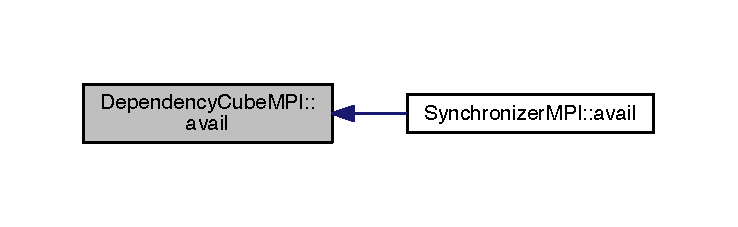
\includegraphics[width=350pt]{d3/d21/class_dependency_cube_m_p_i_a95e03004604866099b5acf0af2cf3b1a_icgraph}
\end{center}
\end{figure}


\hypertarget{class_dependency_cube_m_p_i_a797a6e9d3cb5d7edf9439f4abbf27b05}{}\index{Dependency\+Cube\+M\+P\+I@{Dependency\+Cube\+M\+P\+I}!corner@{corner}}
\index{corner@{corner}!Dependency\+Cube\+M\+P\+I@{Dependency\+Cube\+M\+P\+I}}
\subsubsection[{corner}]{\setlength{\rightskip}{0pt plus 5cm}template$<$typename Request$>$ void {\bf Dependency\+Cube\+M\+P\+I}$<$ Request $>$\+::corner (
\begin{DoxyParamCaption}
\item[{Request}]{req, }
\item[{int}]{x, }
\item[{int}]{y, }
\item[{int}]{z}
\end{DoxyParamCaption}
)\hspace{0.3cm}{\ttfamily [inline]}}\label{class_dependency_cube_m_p_i_a797a6e9d3cb5d7edf9439f4abbf27b05}


Here is the caller graph for this function\+:\nopagebreak
\begin{figure}[H]
\begin{center}
\leavevmode
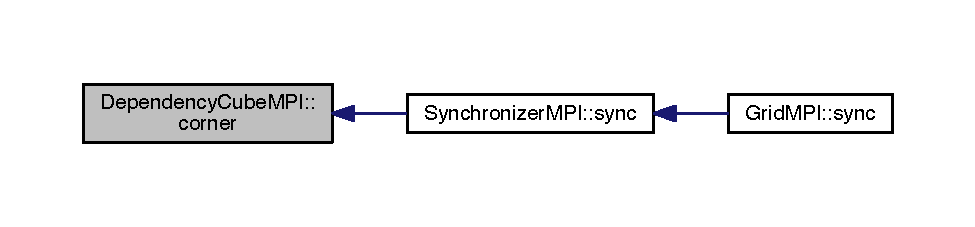
\includegraphics[width=350pt]{d3/d21/class_dependency_cube_m_p_i_a797a6e9d3cb5d7edf9439f4abbf27b05_icgraph}
\end{center}
\end{figure}


\hypertarget{class_dependency_cube_m_p_i_a3c346f1108cb4f571a250b5a6e3cd868}{}\index{Dependency\+Cube\+M\+P\+I@{Dependency\+Cube\+M\+P\+I}!edge@{edge}}
\index{edge@{edge}!Dependency\+Cube\+M\+P\+I@{Dependency\+Cube\+M\+P\+I}}
\subsubsection[{edge}]{\setlength{\rightskip}{0pt plus 5cm}template$<$typename Request$>$ void {\bf Dependency\+Cube\+M\+P\+I}$<$ Request $>$\+::edge (
\begin{DoxyParamCaption}
\item[{Request}]{req, }
\item[{int}]{d, }
\item[{int}]{a, }
\item[{int}]{b}
\end{DoxyParamCaption}
)\hspace{0.3cm}{\ttfamily [inline]}}\label{class_dependency_cube_m_p_i_a3c346f1108cb4f571a250b5a6e3cd868}


Here is the caller graph for this function\+:\nopagebreak
\begin{figure}[H]
\begin{center}
\leavevmode
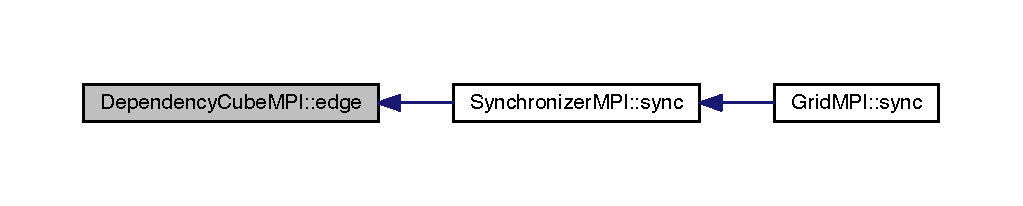
\includegraphics[width=350pt]{d3/d21/class_dependency_cube_m_p_i_a3c346f1108cb4f571a250b5a6e3cd868_icgraph}
\end{center}
\end{figure}


\hypertarget{class_dependency_cube_m_p_i_a057adc047896117c998e5709d8a83d43}{}\index{Dependency\+Cube\+M\+P\+I@{Dependency\+Cube\+M\+P\+I}!face@{face}}
\index{face@{face}!Dependency\+Cube\+M\+P\+I@{Dependency\+Cube\+M\+P\+I}}
\subsubsection[{face}]{\setlength{\rightskip}{0pt plus 5cm}template$<$typename Request$>$ void {\bf Dependency\+Cube\+M\+P\+I}$<$ Request $>$\+::face (
\begin{DoxyParamCaption}
\item[{Request}]{req, }
\item[{int}]{d, }
\item[{int}]{s}
\end{DoxyParamCaption}
)\hspace{0.3cm}{\ttfamily [inline]}}\label{class_dependency_cube_m_p_i_a057adc047896117c998e5709d8a83d43}


Here is the caller graph for this function\+:\nopagebreak
\begin{figure}[H]
\begin{center}
\leavevmode
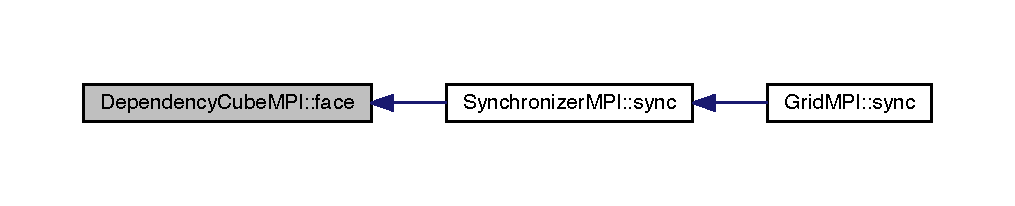
\includegraphics[width=350pt]{d3/d21/class_dependency_cube_m_p_i_a057adc047896117c998e5709d8a83d43_icgraph}
\end{center}
\end{figure}


\hypertarget{class_dependency_cube_m_p_i_a249049eaa66b401dec5b777f91cf14fa}{}\index{Dependency\+Cube\+M\+P\+I@{Dependency\+Cube\+M\+P\+I}!inspect@{inspect}}
\index{inspect@{inspect}!Dependency\+Cube\+M\+P\+I@{Dependency\+Cube\+M\+P\+I}}
\subsubsection[{inspect}]{\setlength{\rightskip}{0pt plus 5cm}template$<$typename Request$>$ void {\bf Dependency\+Cube\+M\+P\+I}$<$ Request $>$\+::inspect (
\begin{DoxyParamCaption}
{}
\end{DoxyParamCaption}
)\hspace{0.3cm}{\ttfamily [inline]}}\label{class_dependency_cube_m_p_i_a249049eaa66b401dec5b777f91cf14fa}
\hypertarget{class_dependency_cube_m_p_i_a65a7562678c7f9d7ab63780ffbdfac87}{}\index{Dependency\+Cube\+M\+P\+I@{Dependency\+Cube\+M\+P\+I}!make\+\_\+dependencies@{make\+\_\+dependencies}}
\index{make\+\_\+dependencies@{make\+\_\+dependencies}!Dependency\+Cube\+M\+P\+I@{Dependency\+Cube\+M\+P\+I}}
\subsubsection[{make\+\_\+dependencies}]{\setlength{\rightskip}{0pt plus 5cm}template$<$typename Request$>$ void {\bf Dependency\+Cube\+M\+P\+I}$<$ Request $>$\+::make\+\_\+dependencies (
\begin{DoxyParamCaption}
\item[{const bool}]{isroot}
\end{DoxyParamCaption}
)\hspace{0.3cm}{\ttfamily [inline]}}\label{class_dependency_cube_m_p_i_a65a7562678c7f9d7ab63780ffbdfac87}


Here is the caller graph for this function\+:\nopagebreak
\begin{figure}[H]
\begin{center}
\leavevmode
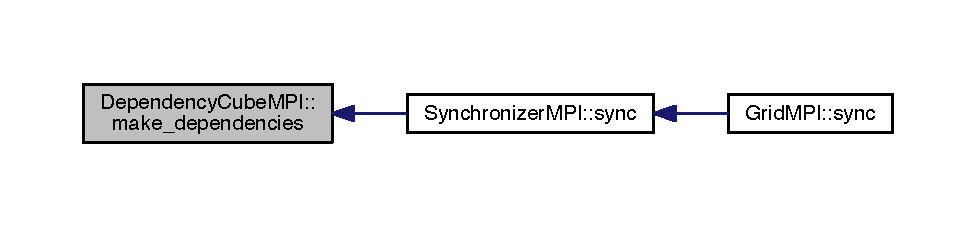
\includegraphics[width=350pt]{d3/d21/class_dependency_cube_m_p_i_a65a7562678c7f9d7ab63780ffbdfac87_icgraph}
\end{center}
\end{figure}


\hypertarget{class_dependency_cube_m_p_i_a9b187ce4ca44a150d71e55c35325afba}{}\index{Dependency\+Cube\+M\+P\+I@{Dependency\+Cube\+M\+P\+I}!pendingcount@{pendingcount}}
\index{pendingcount@{pendingcount}!Dependency\+Cube\+M\+P\+I@{Dependency\+Cube\+M\+P\+I}}
\subsubsection[{pendingcount}]{\setlength{\rightskip}{0pt plus 5cm}template$<$typename Request$>$ int {\bf Dependency\+Cube\+M\+P\+I}$<$ Request $>$\+::pendingcount (
\begin{DoxyParamCaption}
{}
\end{DoxyParamCaption}
) const\hspace{0.3cm}{\ttfamily [inline]}}\label{class_dependency_cube_m_p_i_a9b187ce4ca44a150d71e55c35325afba}


Here is the caller graph for this function\+:\nopagebreak
\begin{figure}[H]
\begin{center}
\leavevmode
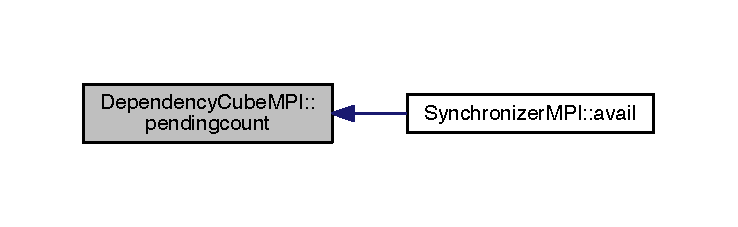
\includegraphics[width=350pt]{d3/d21/class_dependency_cube_m_p_i_a9b187ce4ca44a150d71e55c35325afba_icgraph}
\end{center}
\end{figure}


\hypertarget{class_dependency_cube_m_p_i_abd4e8187ccfe651ded18f8c5c10fa691}{}\index{Dependency\+Cube\+M\+P\+I@{Dependency\+Cube\+M\+P\+I}!prepare@{prepare}}
\index{prepare@{prepare}!Dependency\+Cube\+M\+P\+I@{Dependency\+Cube\+M\+P\+I}}
\subsubsection[{prepare}]{\setlength{\rightskip}{0pt plus 5cm}template$<$typename Request$>$ void {\bf Dependency\+Cube\+M\+P\+I}$<$ Request $>$\+::prepare (
\begin{DoxyParamCaption}
{}
\end{DoxyParamCaption}
)\hspace{0.3cm}{\ttfamily [inline]}}\label{class_dependency_cube_m_p_i_abd4e8187ccfe651ded18f8c5c10fa691}


Here is the caller graph for this function\+:\nopagebreak
\begin{figure}[H]
\begin{center}
\leavevmode
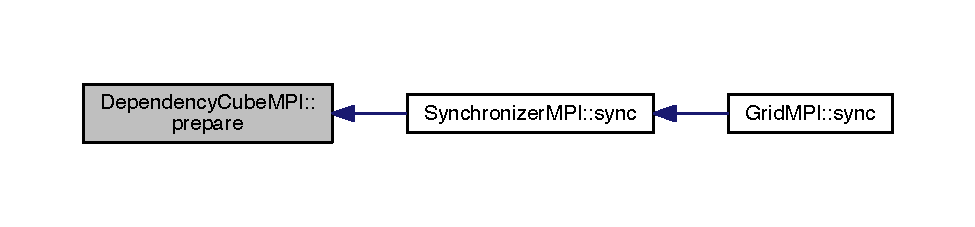
\includegraphics[width=350pt]{d3/d21/class_dependency_cube_m_p_i_abd4e8187ccfe651ded18f8c5c10fa691_icgraph}
\end{center}
\end{figure}


\hypertarget{class_dependency_cube_m_p_i_a6b7972db814a3469a2774946ba3062a4}{}\index{Dependency\+Cube\+M\+P\+I@{Dependency\+Cube\+M\+P\+I}!received@{received}}
\index{received@{received}!Dependency\+Cube\+M\+P\+I@{Dependency\+Cube\+M\+P\+I}}
\subsubsection[{received}]{\setlength{\rightskip}{0pt plus 5cm}template$<$typename Request$>$ void {\bf Dependency\+Cube\+M\+P\+I}$<$ Request $>$\+::received (
\begin{DoxyParamCaption}
\item[{Request}]{req}
\end{DoxyParamCaption}
)\hspace{0.3cm}{\ttfamily [inline]}}\label{class_dependency_cube_m_p_i_a6b7972db814a3469a2774946ba3062a4}


Here is the caller graph for this function\+:\nopagebreak
\begin{figure}[H]
\begin{center}
\leavevmode
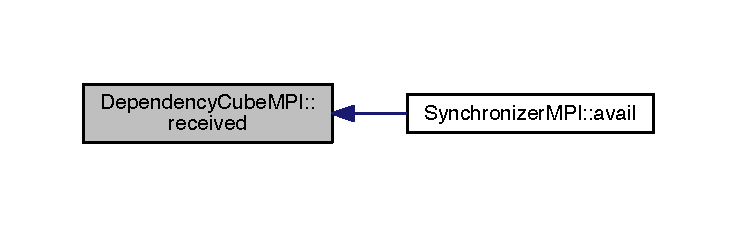
\includegraphics[width=350pt]{d3/d21/class_dependency_cube_m_p_i_a6b7972db814a3469a2774946ba3062a4_icgraph}
\end{center}
\end{figure}




\subsection{Member Data Documentation}
\hypertarget{class_dependency_cube_m_p_i_a4996ead8bdfbf954562d0177b6c24607}{}\index{Dependency\+Cube\+M\+P\+I@{Dependency\+Cube\+M\+P\+I}!all\+\_\+pending@{all\+\_\+pending}}
\index{all\+\_\+pending@{all\+\_\+pending}!Dependency\+Cube\+M\+P\+I@{Dependency\+Cube\+M\+P\+I}}
\subsubsection[{all\+\_\+pending}]{\setlength{\rightskip}{0pt plus 5cm}template$<$typename Request$>$ set$<$Request$>$ {\bf Dependency\+Cube\+M\+P\+I}$<$ Request $>$\+::all\+\_\+pending}\label{class_dependency_cube_m_p_i_a4996ead8bdfbf954562d0177b6c24607}
\hypertarget{class_dependency_cube_m_p_i_a79cbdbeafcdad83edcfe7bfb786e8dbb}{}\index{Dependency\+Cube\+M\+P\+I@{Dependency\+Cube\+M\+P\+I}!finalized@{finalized}}
\index{finalized@{finalized}!Dependency\+Cube\+M\+P\+I@{Dependency\+Cube\+M\+P\+I}}
\subsubsection[{finalized}]{\setlength{\rightskip}{0pt plus 5cm}template$<$typename Request$>$ bool {\bf Dependency\+Cube\+M\+P\+I}$<$ Request $>$\+::finalized}\label{class_dependency_cube_m_p_i_a79cbdbeafcdad83edcfe7bfb786e8dbb}
\hypertarget{class_dependency_cube_m_p_i_a15e719dff5340ab953286ba4b9301a54}{}\index{Dependency\+Cube\+M\+P\+I@{Dependency\+Cube\+M\+P\+I}!pending@{pending}}
\index{pending@{pending}!Dependency\+Cube\+M\+P\+I@{Dependency\+Cube\+M\+P\+I}}
\subsubsection[{pending}]{\setlength{\rightskip}{0pt plus 5cm}template$<$typename Request$>$ map$<${\bf Region}, set$<$Request$>$ $>$ {\bf Dependency\+Cube\+M\+P\+I}$<$ Request $>$\+::pending}\label{class_dependency_cube_m_p_i_a15e719dff5340ab953286ba4b9301a54}


The documentation for this class was generated from the following file\+:\begin{DoxyCompactItemize}
\item 
Cubism/\hyperlink{_dependency_cube_m_p_i_8h}{Dependency\+Cube\+M\+P\+I.\+h}\end{DoxyCompactItemize}

\hypertarget{class_disk}{}\section{Disk Class Reference}
\label{class_disk}\index{Disk@{Disk}}


{\ttfamily \#include $<$Shape.\+h$>$}



Inheritance diagram for Disk\+:
% FIG 0


Collaboration diagram for Disk\+:
% FIG 1
\subsection*{Public Member Functions}
\begin{DoxyCompactItemize}
\item 
\hyperlink{class_disk_a5ea7dc49cd7d0685989c63e64ab3b71f}{Disk} (\hyperlink{_h_d_f5_dumper_8h_a445a5f0e2a34c9d97d69a3c2d1957907}{Real} \hyperlink{class_shape_a865a04fe67fc785b3cbb44806a214248}{center}\mbox{[}2\mbox{]}, \hyperlink{_h_d_f5_dumper_8h_a445a5f0e2a34c9d97d69a3c2d1957907}{Real} \hyperlink{class_disk_ae6a9adac6c5dd96d63d0a3345f90499d}{radius}, const \hyperlink{_h_d_f5_dumper_8h_a445a5f0e2a34c9d97d69a3c2d1957907}{Real} \hyperlink{class_shape_a181acdc3063f20a15ba1807f7b6a5d10}{rho\+S}, const \hyperlink{_h_d_f5_dumper_8h_a445a5f0e2a34c9d97d69a3c2d1957907}{Real} \hyperlink{class_shape_ad7d270a8ffc4056d4990424dffdd0488}{moll\+Chi}, const \hyperlink{_h_d_f5_dumper_8h_a445a5f0e2a34c9d97d69a3c2d1957907}{Real} \hyperlink{class_shape_af5aa25175d49bc463fada7b11f2735e1}{moll\+Rho})
\item 
\hyperlink{_h_d_f5_dumper_8h_a445a5f0e2a34c9d97d69a3c2d1957907}{Real} \hyperlink{class_disk_afccc38b335adb2268cc7955da02da0f2}{chi} (\hyperlink{_h_d_f5_dumper_8h_a445a5f0e2a34c9d97d69a3c2d1957907}{Real} p\mbox{[}2\mbox{]})
\item 
\hyperlink{_h_d_f5_dumper_8h_a445a5f0e2a34c9d97d69a3c2d1957907}{Real} \hyperlink{class_disk_a55ef38503419802fe0b8feea43a3f215}{rho} (\hyperlink{_h_d_f5_dumper_8h_a445a5f0e2a34c9d97d69a3c2d1957907}{Real} p\mbox{[}2\mbox{]})
\end{DoxyCompactItemize}
\subsection*{Protected Member Functions}
\begin{DoxyCompactItemize}
\item 
\hyperlink{_h_d_f5_dumper_8h_a445a5f0e2a34c9d97d69a3c2d1957907}{Real} \hyperlink{class_disk_ab7f65af10857217606c73f7b598da9a4}{smooth\+Heaviside} (\hyperlink{_h_d_f5_dumper_8h_a445a5f0e2a34c9d97d69a3c2d1957907}{Real} r\+R, \hyperlink{_h_d_f5_dumper_8h_a445a5f0e2a34c9d97d69a3c2d1957907}{Real} \hyperlink{class_disk_ae6a9adac6c5dd96d63d0a3345f90499d}{radius}, \hyperlink{_h_d_f5_dumper_8h_a445a5f0e2a34c9d97d69a3c2d1957907}{Real} eps)
\end{DoxyCompactItemize}
\subsection*{Protected Attributes}
\begin{DoxyCompactItemize}
\item 
\hyperlink{_h_d_f5_dumper_8h_a445a5f0e2a34c9d97d69a3c2d1957907}{Real} \hyperlink{class_disk_ae6a9adac6c5dd96d63d0a3345f90499d}{radius}
\end{DoxyCompactItemize}


\subsection{Constructor \& Destructor Documentation}
\hypertarget{class_disk_a5ea7dc49cd7d0685989c63e64ab3b71f}{}\index{Disk@{Disk}!Disk@{Disk}}
\index{Disk@{Disk}!Disk@{Disk}}
\subsubsection[{Disk}]{\setlength{\rightskip}{0pt plus 5cm}Disk\+::\+Disk (
\begin{DoxyParamCaption}
\item[{{\bf Real}}]{center\mbox{[}2\mbox{]}, }
\item[{{\bf Real}}]{radius, }
\item[{const {\bf Real}}]{rho\+S, }
\item[{const {\bf Real}}]{moll\+Chi, }
\item[{const {\bf Real}}]{moll\+Rho}
\end{DoxyParamCaption}
)\hspace{0.3cm}{\ttfamily [inline]}}\label{class_disk_a5ea7dc49cd7d0685989c63e64ab3b71f}


\subsection{Member Function Documentation}
\hypertarget{class_disk_afccc38b335adb2268cc7955da02da0f2}{}\index{Disk@{Disk}!chi@{chi}}
\index{chi@{chi}!Disk@{Disk}}
\subsubsection[{chi}]{\setlength{\rightskip}{0pt plus 5cm}{\bf Real} Disk\+::chi (
\begin{DoxyParamCaption}
\item[{{\bf Real}}]{p\mbox{[}2\mbox{]}}
\end{DoxyParamCaption}
)\hspace{0.3cm}{\ttfamily [inline]}, {\ttfamily [virtual]}}\label{class_disk_afccc38b335adb2268cc7955da02da0f2}


Implements \hyperlink{class_shape_a4f73c637114b82612ba4cfde42886f25}{Shape}.



Here is the call graph for this function\+:
% FIG 2


\hypertarget{class_disk_a55ef38503419802fe0b8feea43a3f215}{}\index{Disk@{Disk}!rho@{rho}}
\index{rho@{rho}!Disk@{Disk}}
\subsubsection[{rho}]{\setlength{\rightskip}{0pt plus 5cm}{\bf Real} Disk\+::rho (
\begin{DoxyParamCaption}
\item[{{\bf Real}}]{p\mbox{[}2\mbox{]}}
\end{DoxyParamCaption}
)\hspace{0.3cm}{\ttfamily [inline]}, {\ttfamily [virtual]}}\label{class_disk_a55ef38503419802fe0b8feea43a3f215}


Implements \hyperlink{class_shape_af55591d6633578cbea6132f52d104cdb}{Shape}.



Here is the call graph for this function\+:
% FIG 3


\hypertarget{class_disk_ab7f65af10857217606c73f7b598da9a4}{}\index{Disk@{Disk}!smooth\+Heaviside@{smooth\+Heaviside}}
\index{smooth\+Heaviside@{smooth\+Heaviside}!Disk@{Disk}}
\subsubsection[{smooth\+Heaviside}]{\setlength{\rightskip}{0pt plus 5cm}{\bf Real} Disk\+::smooth\+Heaviside (
\begin{DoxyParamCaption}
\item[{{\bf Real}}]{r\+R, }
\item[{{\bf Real}}]{radius, }
\item[{{\bf Real}}]{eps}
\end{DoxyParamCaption}
)\hspace{0.3cm}{\ttfamily [inline]}, {\ttfamily [protected]}}\label{class_disk_ab7f65af10857217606c73f7b598da9a4}


Here is the caller graph for this function\+:
% FIG 4




\subsection{Member Data Documentation}
\hypertarget{class_disk_ae6a9adac6c5dd96d63d0a3345f90499d}{}\index{Disk@{Disk}!radius@{radius}}
\index{radius@{radius}!Disk@{Disk}}
\subsubsection[{radius}]{\setlength{\rightskip}{0pt plus 5cm}{\bf Real} Disk\+::radius\hspace{0.3cm}{\ttfamily [protected]}}\label{class_disk_ae6a9adac6c5dd96d63d0a3345f90499d}


The documentation for this class was generated from the following file\+:\begin{DoxyCompactItemize}
\item 
/\+Users/cconti/\+Desktop/\+Mounts/\+Brutus\+Home/\+Seed/\+Cubism\+U\+P\+\_\+2\+D/source/\hyperlink{_shape_8h}{Shape.\+h}\end{DoxyCompactItemize}

\hypertarget{struct_dependency_cube_m_p_i_1_1_edge}{}\section{Dependency\+Cube\+M\+P\+I$<$ Request $>$\+:\+:Edge Struct Reference}
\label{struct_dependency_cube_m_p_i_1_1_edge}\index{Dependency\+Cube\+M\+P\+I$<$ Request $>$\+::\+Edge@{Dependency\+Cube\+M\+P\+I$<$ Request $>$\+::\+Edge}}


{\ttfamily \#include $<$Dependency\+Cube\+M\+P\+I.\+h$>$}



Inheritance diagram for Dependency\+Cube\+M\+P\+I$<$ Request $>$\+:\+:Edge\+:\nopagebreak
\begin{figure}[H]
\begin{center}
\leavevmode
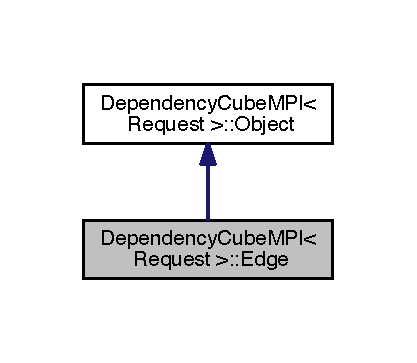
\includegraphics[width=200pt]{d0/dad/struct_dependency_cube_m_p_i_1_1_edge__inherit__graph}
\end{center}
\end{figure}


Collaboration diagram for Dependency\+Cube\+M\+P\+I$<$ Request $>$\+:\+:Edge\+:\nopagebreak
\begin{figure}[H]
\begin{center}
\leavevmode
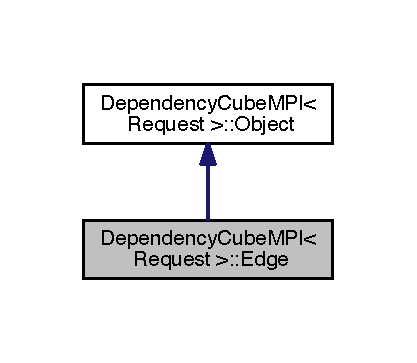
\includegraphics[width=200pt]{d1/d32/struct_dependency_cube_m_p_i_1_1_edge__coll__graph}
\end{center}
\end{figure}
\subsection*{Public Member Functions}
\begin{DoxyCompactItemize}
\item 
\hyperlink{struct_dependency_cube_m_p_i_1_1_edge_a4300ae373dfb130d69654ba7dc54b42c}{Edge} ()
\item 
\hyperlink{struct_dependency_cube_m_p_i_1_1_edge_aa9e7ee251e0259c647dc41a193e1cf6f}{Edge} (Direction \hyperlink{struct_dependency_cube_m_p_i_1_1_edge_a8669784b9f597960def87cc96ebd0e1f}{d}, Side \hyperlink{struct_dependency_cube_m_p_i_1_1_edge_a08c5f45fa42aa4b3d2177c07f00eb076}{a}, Side \hyperlink{struct_dependency_cube_m_p_i_1_1_edge_a017525e4ab3ec35aa19a4de2c7b6ebc1}{b})
\item 
\hyperlink{struct_dependency_cube_m_p_i_1_1_edge}{Edge} \& \hyperlink{struct_dependency_cube_m_p_i_1_1_edge_a5c268dbc2c12757dadfc0416efc468a1}{operator=} (const \hyperlink{struct_dependency_cube_m_p_i_1_1_edge}{Edge} \&f)
\item 
\hyperlink{struct_region}{Region} \hyperlink{struct_dependency_cube_m_p_i_1_1_edge_a8964aa3679c17660a3647a83514c348d}{get\+Region} (const int n\mbox{[}3\mbox{]})
\end{DoxyCompactItemize}
\subsection*{Public Attributes}
\begin{DoxyCompactItemize}
\item 
Direction \hyperlink{struct_dependency_cube_m_p_i_1_1_edge_a8669784b9f597960def87cc96ebd0e1f}{d}
\item 
Side \hyperlink{struct_dependency_cube_m_p_i_1_1_edge_a08c5f45fa42aa4b3d2177c07f00eb076}{a}
\item 
Side \hyperlink{struct_dependency_cube_m_p_i_1_1_edge_a017525e4ab3ec35aa19a4de2c7b6ebc1}{b}
\end{DoxyCompactItemize}


\subsection{Constructor \& Destructor Documentation}
\hypertarget{struct_dependency_cube_m_p_i_1_1_edge_a4300ae373dfb130d69654ba7dc54b42c}{}\index{Dependency\+Cube\+M\+P\+I\+::\+Edge@{Dependency\+Cube\+M\+P\+I\+::\+Edge}!Edge@{Edge}}
\index{Edge@{Edge}!Dependency\+Cube\+M\+P\+I\+::\+Edge@{Dependency\+Cube\+M\+P\+I\+::\+Edge}}
\subsubsection[{Edge}]{\setlength{\rightskip}{0pt plus 5cm}template$<$typename Request$>$ {\bf Dependency\+Cube\+M\+P\+I}$<$ Request $>$\+::Edge\+::\+Edge (
\begin{DoxyParamCaption}
{}
\end{DoxyParamCaption}
)\hspace{0.3cm}{\ttfamily [inline]}}\label{struct_dependency_cube_m_p_i_1_1_edge_a4300ae373dfb130d69654ba7dc54b42c}
\hypertarget{struct_dependency_cube_m_p_i_1_1_edge_aa9e7ee251e0259c647dc41a193e1cf6f}{}\index{Dependency\+Cube\+M\+P\+I\+::\+Edge@{Dependency\+Cube\+M\+P\+I\+::\+Edge}!Edge@{Edge}}
\index{Edge@{Edge}!Dependency\+Cube\+M\+P\+I\+::\+Edge@{Dependency\+Cube\+M\+P\+I\+::\+Edge}}
\subsubsection[{Edge}]{\setlength{\rightskip}{0pt plus 5cm}template$<$typename Request$>$ {\bf Dependency\+Cube\+M\+P\+I}$<$ Request $>$\+::Edge\+::\+Edge (
\begin{DoxyParamCaption}
\item[{Direction}]{d, }
\item[{Side}]{a, }
\item[{Side}]{b}
\end{DoxyParamCaption}
)\hspace{0.3cm}{\ttfamily [inline]}}\label{struct_dependency_cube_m_p_i_1_1_edge_aa9e7ee251e0259c647dc41a193e1cf6f}


\subsection{Member Function Documentation}
\hypertarget{struct_dependency_cube_m_p_i_1_1_edge_a8964aa3679c17660a3647a83514c348d}{}\index{Dependency\+Cube\+M\+P\+I\+::\+Edge@{Dependency\+Cube\+M\+P\+I\+::\+Edge}!get\+Region@{get\+Region}}
\index{get\+Region@{get\+Region}!Dependency\+Cube\+M\+P\+I\+::\+Edge@{Dependency\+Cube\+M\+P\+I\+::\+Edge}}
\subsubsection[{get\+Region}]{\setlength{\rightskip}{0pt plus 5cm}template$<$typename Request$>$ {\bf Region} {\bf Dependency\+Cube\+M\+P\+I}$<$ Request $>$\+::Edge\+::get\+Region (
\begin{DoxyParamCaption}
\item[{const int}]{n\mbox{[}3\mbox{]}}
\end{DoxyParamCaption}
)\hspace{0.3cm}{\ttfamily [inline]}}\label{struct_dependency_cube_m_p_i_1_1_edge_a8964aa3679c17660a3647a83514c348d}
\hypertarget{struct_dependency_cube_m_p_i_1_1_edge_a5c268dbc2c12757dadfc0416efc468a1}{}\index{Dependency\+Cube\+M\+P\+I\+::\+Edge@{Dependency\+Cube\+M\+P\+I\+::\+Edge}!operator=@{operator=}}
\index{operator=@{operator=}!Dependency\+Cube\+M\+P\+I\+::\+Edge@{Dependency\+Cube\+M\+P\+I\+::\+Edge}}
\subsubsection[{operator=}]{\setlength{\rightskip}{0pt plus 5cm}template$<$typename Request$>$ {\bf Edge}\& {\bf Dependency\+Cube\+M\+P\+I}$<$ Request $>$\+::Edge\+::operator= (
\begin{DoxyParamCaption}
\item[{const {\bf Edge} \&}]{f}
\end{DoxyParamCaption}
)\hspace{0.3cm}{\ttfamily [inline]}}\label{struct_dependency_cube_m_p_i_1_1_edge_a5c268dbc2c12757dadfc0416efc468a1}


\subsection{Member Data Documentation}
\hypertarget{struct_dependency_cube_m_p_i_1_1_edge_a08c5f45fa42aa4b3d2177c07f00eb076}{}\index{Dependency\+Cube\+M\+P\+I\+::\+Edge@{Dependency\+Cube\+M\+P\+I\+::\+Edge}!a@{a}}
\index{a@{a}!Dependency\+Cube\+M\+P\+I\+::\+Edge@{Dependency\+Cube\+M\+P\+I\+::\+Edge}}
\subsubsection[{a}]{\setlength{\rightskip}{0pt plus 5cm}template$<$typename Request$>$ Side {\bf Dependency\+Cube\+M\+P\+I}$<$ Request $>$\+::Edge\+::a}\label{struct_dependency_cube_m_p_i_1_1_edge_a08c5f45fa42aa4b3d2177c07f00eb076}
\hypertarget{struct_dependency_cube_m_p_i_1_1_edge_a017525e4ab3ec35aa19a4de2c7b6ebc1}{}\index{Dependency\+Cube\+M\+P\+I\+::\+Edge@{Dependency\+Cube\+M\+P\+I\+::\+Edge}!b@{b}}
\index{b@{b}!Dependency\+Cube\+M\+P\+I\+::\+Edge@{Dependency\+Cube\+M\+P\+I\+::\+Edge}}
\subsubsection[{b}]{\setlength{\rightskip}{0pt plus 5cm}template$<$typename Request$>$ Side {\bf Dependency\+Cube\+M\+P\+I}$<$ Request $>$\+::Edge\+::b}\label{struct_dependency_cube_m_p_i_1_1_edge_a017525e4ab3ec35aa19a4de2c7b6ebc1}
\hypertarget{struct_dependency_cube_m_p_i_1_1_edge_a8669784b9f597960def87cc96ebd0e1f}{}\index{Dependency\+Cube\+M\+P\+I\+::\+Edge@{Dependency\+Cube\+M\+P\+I\+::\+Edge}!d@{d}}
\index{d@{d}!Dependency\+Cube\+M\+P\+I\+::\+Edge@{Dependency\+Cube\+M\+P\+I\+::\+Edge}}
\subsubsection[{d}]{\setlength{\rightskip}{0pt plus 5cm}template$<$typename Request$>$ Direction {\bf Dependency\+Cube\+M\+P\+I}$<$ Request $>$\+::Edge\+::d}\label{struct_dependency_cube_m_p_i_1_1_edge_a8669784b9f597960def87cc96ebd0e1f}


The documentation for this struct was generated from the following file\+:\begin{DoxyCompactItemize}
\item 
/\+Users/cconti/\+Desktop/\+Mounts/\+Brutus\+Home/\+Cubism\+U\+P\+\_\+2\+D/\+Cubism/\hyperlink{_dependency_cube_m_p_i_8h}{Dependency\+Cube\+M\+P\+I.\+h}\end{DoxyCompactItemize}

\hypertarget{class_ellipse}{}\section{Ellipse Class Reference}
\label{class_ellipse}\index{Ellipse@{Ellipse}}


{\ttfamily \#include $<$Shape.\+h$>$}



Inheritance diagram for Ellipse\+:\nopagebreak
\begin{figure}[H]
\begin{center}
\leavevmode
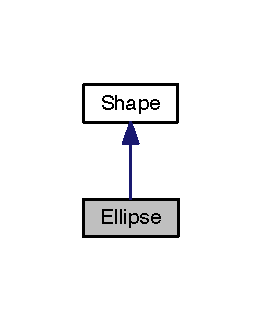
\includegraphics[width=125pt]{dd/ddc/class_ellipse__inherit__graph}
\end{center}
\end{figure}


Collaboration diagram for Ellipse\+:\nopagebreak
\begin{figure}[H]
\begin{center}
\leavevmode
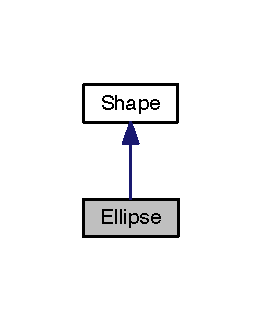
\includegraphics[width=125pt]{d4/df4/class_ellipse__coll__graph}
\end{center}
\end{figure}
\subsection*{Public Member Functions}
\begin{DoxyCompactItemize}
\item 
\hyperlink{class_ellipse_a0deee753167fddaf46ee4069f6163d75}{Ellipse} (\hyperlink{_h_d_f5_dumper_8h_a445a5f0e2a34c9d97d69a3c2d1957907}{Real} \hyperlink{class_shape_a865a04fe67fc785b3cbb44806a214248}{center}\mbox{[}2\mbox{]}, \hyperlink{_h_d_f5_dumper_8h_a445a5f0e2a34c9d97d69a3c2d1957907}{Real} \hyperlink{class_ellipse_aa4758f568a38a31bbea0b4b424486a40}{semi\+Axis}\mbox{[}2\mbox{]}, \hyperlink{_h_d_f5_dumper_8h_a445a5f0e2a34c9d97d69a3c2d1957907}{Real} \hyperlink{class_shape_a1778439509ada1f3fa64472610221d19}{orientation}, const \hyperlink{_h_d_f5_dumper_8h_a445a5f0e2a34c9d97d69a3c2d1957907}{Real} \hyperlink{class_shape_a181acdc3063f20a15ba1807f7b6a5d10}{rho\+S}, const \hyperlink{_h_d_f5_dumper_8h_a445a5f0e2a34c9d97d69a3c2d1957907}{Real} \hyperlink{class_shape_ad7d270a8ffc4056d4990424dffdd0488}{moll\+Chi}, const \hyperlink{_h_d_f5_dumper_8h_a445a5f0e2a34c9d97d69a3c2d1957907}{Real} \hyperlink{class_shape_af5aa25175d49bc463fada7b11f2735e1}{moll\+Rho}, bool b\+Periodic\mbox{[}2\mbox{]})
\item 
\hyperlink{_h_d_f5_dumper_8h_a445a5f0e2a34c9d97d69a3c2d1957907}{Real} \hyperlink{class_ellipse_ab4cc2d14593c52c17a78d9d2a7f4ecb9}{chi} (\hyperlink{_h_d_f5_dumper_8h_a445a5f0e2a34c9d97d69a3c2d1957907}{Real} p\mbox{[}2\mbox{]}, \hyperlink{_h_d_f5_dumper_8h_a445a5f0e2a34c9d97d69a3c2d1957907}{Real} h) const 
\item 
\hyperlink{_h_d_f5_dumper_8h_a445a5f0e2a34c9d97d69a3c2d1957907}{Real} \hyperlink{class_ellipse_a51028b0d38b83fc0de8c60c27775ed14}{get\+Char\+Length} () const 
\end{DoxyCompactItemize}
\subsection*{Protected Attributes}
\begin{DoxyCompactItemize}
\item 
\hyperlink{_h_d_f5_dumper_8h_a445a5f0e2a34c9d97d69a3c2d1957907}{Real} \hyperlink{class_ellipse_aa4758f568a38a31bbea0b4b424486a40}{semi\+Axis} \mbox{[}2\mbox{]}
\end{DoxyCompactItemize}
\subsection*{Additional Inherited Members}


\subsection{Constructor \& Destructor Documentation}
\hypertarget{class_ellipse_a0deee753167fddaf46ee4069f6163d75}{}\index{Ellipse@{Ellipse}!Ellipse@{Ellipse}}
\index{Ellipse@{Ellipse}!Ellipse@{Ellipse}}
\subsubsection[{Ellipse}]{\setlength{\rightskip}{0pt plus 5cm}Ellipse\+::\+Ellipse (
\begin{DoxyParamCaption}
\item[{{\bf Real}}]{center\mbox{[}2\mbox{]}, }
\item[{{\bf Real}}]{semi\+Axis\mbox{[}2\mbox{]}, }
\item[{{\bf Real}}]{orientation, }
\item[{const {\bf Real}}]{rho\+S, }
\item[{const {\bf Real}}]{moll\+Chi, }
\item[{const {\bf Real}}]{moll\+Rho, }
\item[{bool}]{b\+Periodic\mbox{[}2\mbox{]}}
\end{DoxyParamCaption}
)\hspace{0.3cm}{\ttfamily [inline]}}\label{class_ellipse_a0deee753167fddaf46ee4069f6163d75}


\subsection{Member Function Documentation}
\hypertarget{class_ellipse_ab4cc2d14593c52c17a78d9d2a7f4ecb9}{}\index{Ellipse@{Ellipse}!chi@{chi}}
\index{chi@{chi}!Ellipse@{Ellipse}}
\subsubsection[{chi}]{\setlength{\rightskip}{0pt plus 5cm}{\bf Real} Ellipse\+::chi (
\begin{DoxyParamCaption}
\item[{{\bf Real}}]{p\mbox{[}2\mbox{]}, }
\item[{{\bf Real}}]{h}
\end{DoxyParamCaption}
) const\hspace{0.3cm}{\ttfamily [inline]}, {\ttfamily [virtual]}}\label{class_ellipse_ab4cc2d14593c52c17a78d9d2a7f4ecb9}


Implements \hyperlink{class_shape_aafa14cb6631bdc7a7a775e83a4bf5cdf}{Shape}.



Here is the call graph for this function\+:\nopagebreak
\begin{figure}[H]
\begin{center}
\leavevmode
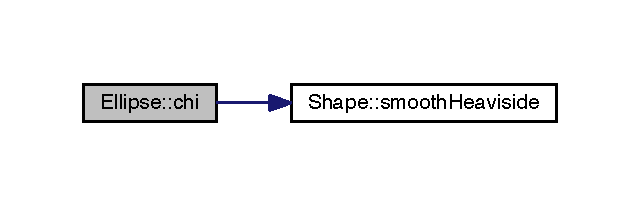
\includegraphics[width=307pt]{dc/d25/class_ellipse_ab4cc2d14593c52c17a78d9d2a7f4ecb9_cgraph}
\end{center}
\end{figure}


\hypertarget{class_ellipse_a51028b0d38b83fc0de8c60c27775ed14}{}\index{Ellipse@{Ellipse}!get\+Char\+Length@{get\+Char\+Length}}
\index{get\+Char\+Length@{get\+Char\+Length}!Ellipse@{Ellipse}}
\subsubsection[{get\+Char\+Length}]{\setlength{\rightskip}{0pt plus 5cm}{\bf Real} Ellipse\+::get\+Char\+Length (
\begin{DoxyParamCaption}
{}
\end{DoxyParamCaption}
) const\hspace{0.3cm}{\ttfamily [inline]}, {\ttfamily [virtual]}}\label{class_ellipse_a51028b0d38b83fc0de8c60c27775ed14}


Implements \hyperlink{class_shape_a702acbc7c7ac03d89a994404569f173f}{Shape}.



\subsection{Member Data Documentation}
\hypertarget{class_ellipse_aa4758f568a38a31bbea0b4b424486a40}{}\index{Ellipse@{Ellipse}!semi\+Axis@{semi\+Axis}}
\index{semi\+Axis@{semi\+Axis}!Ellipse@{Ellipse}}
\subsubsection[{semi\+Axis}]{\setlength{\rightskip}{0pt plus 5cm}{\bf Real} Ellipse\+::semi\+Axis\mbox{[}2\mbox{]}\hspace{0.3cm}{\ttfamily [protected]}}\label{class_ellipse_aa4758f568a38a31bbea0b4b424486a40}


The documentation for this class was generated from the following file\+:\begin{DoxyCompactItemize}
\item 
source/\hyperlink{_shape_8h}{Shape.\+h}\end{DoxyCompactItemize}

\hypertarget{class_empty_block_lab}{}\section{Empty\+Block\+Lab$<$ Block\+Type, allocator, Element\+Type\+T $>$ Class Template Reference}
\label{class_empty_block_lab}\index{Empty\+Block\+Lab$<$ Block\+Type, allocator, Element\+Type\+T $>$@{Empty\+Block\+Lab$<$ Block\+Type, allocator, Element\+Type\+T $>$}}


{\ttfamily \#include $<$Block\+Lab.\+h$>$}



Inheritance diagram for Empty\+Block\+Lab$<$ Block\+Type, allocator, Element\+Type\+T $>$\+:\nopagebreak
\begin{figure}[H]
\begin{center}
\leavevmode
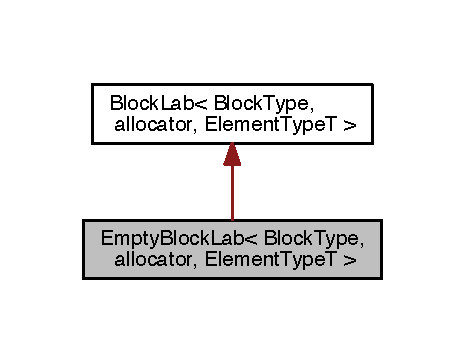
\includegraphics[width=223pt]{d9/d4f/class_empty_block_lab__inherit__graph}
\end{center}
\end{figure}


Collaboration diagram for Empty\+Block\+Lab$<$ Block\+Type, allocator, Element\+Type\+T $>$\+:\nopagebreak
\begin{figure}[H]
\begin{center}
\leavevmode
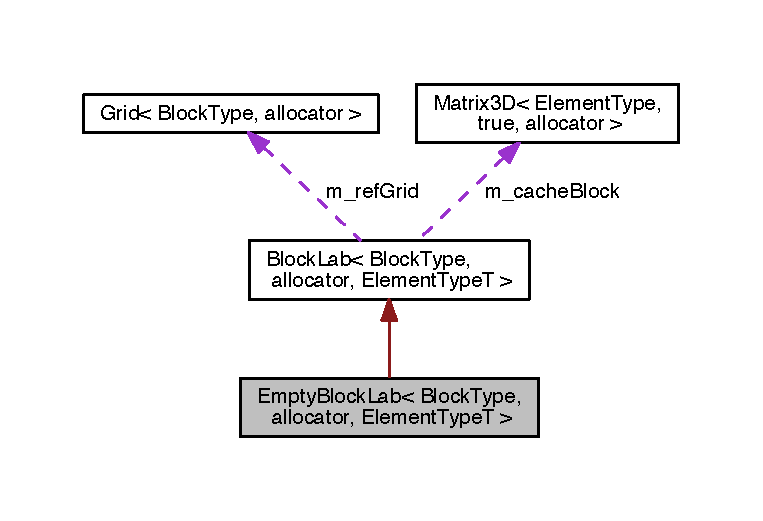
\includegraphics[width=350pt]{d8/df4/class_empty_block_lab__coll__graph}
\end{center}
\end{figure}
\subsection*{Public Types}
\begin{DoxyCompactItemize}
\item 
typedef Element\+Type\+T \hyperlink{class_empty_block_lab_a090310d2af6fb159b6fe949413cbd47a}{Element\+Type}
\end{DoxyCompactItemize}
\subsection*{Public Member Functions}
\begin{DoxyCompactItemize}
\item 
\hyperlink{class_empty_block_lab_a8311d174957e8254a665b5b23c38e844}{Empty\+Block\+Lab} ()
\item 
void \hyperlink{class_empty_block_lab_acc1e6ead590c67446bee384eb3a3ec49}{prepare} (\hyperlink{class_grid}{Grid}$<$ \hyperlink{class_block_lab_a745b3c9ac17f6743d11a7085196981a0}{Block\+Type}, allocator $>$ \&grid, const int stencil\+\_\+start\mbox{[}3\mbox{]}, const int stencil\+\_\+end\mbox{[}3\mbox{]})
\end{DoxyCompactItemize}


\subsection{Member Typedef Documentation}
\hypertarget{class_empty_block_lab_a090310d2af6fb159b6fe949413cbd47a}{}\index{Empty\+Block\+Lab@{Empty\+Block\+Lab}!Element\+Type@{Element\+Type}}
\index{Element\+Type@{Element\+Type}!Empty\+Block\+Lab@{Empty\+Block\+Lab}}
\subsubsection[{Element\+Type}]{\setlength{\rightskip}{0pt plus 5cm}template$<$typename Block\+Type , template$<$ typename X $>$ class allocator = std\+::allocator, typename Element\+Type\+T  = typename Block\+Type\+::\+Element\+Type$>$ typedef Element\+Type\+T {\bf Empty\+Block\+Lab}$<$ {\bf Block\+Type}, allocator, Element\+Type\+T $>$\+::{\bf Element\+Type}}\label{class_empty_block_lab_a090310d2af6fb159b6fe949413cbd47a}


\subsection{Constructor \& Destructor Documentation}
\hypertarget{class_empty_block_lab_a8311d174957e8254a665b5b23c38e844}{}\index{Empty\+Block\+Lab@{Empty\+Block\+Lab}!Empty\+Block\+Lab@{Empty\+Block\+Lab}}
\index{Empty\+Block\+Lab@{Empty\+Block\+Lab}!Empty\+Block\+Lab@{Empty\+Block\+Lab}}
\subsubsection[{Empty\+Block\+Lab}]{\setlength{\rightskip}{0pt plus 5cm}template$<$typename Block\+Type , template$<$ typename X $>$ class allocator = std\+::allocator, typename Element\+Type\+T  = typename Block\+Type\+::\+Element\+Type$>$ {\bf Empty\+Block\+Lab}$<$ {\bf Block\+Type}, allocator, Element\+Type\+T $>$\+::{\bf Empty\+Block\+Lab} (
\begin{DoxyParamCaption}
{}
\end{DoxyParamCaption}
)\hspace{0.3cm}{\ttfamily [inline]}}\label{class_empty_block_lab_a8311d174957e8254a665b5b23c38e844}


\subsection{Member Function Documentation}
\hypertarget{class_empty_block_lab_acc1e6ead590c67446bee384eb3a3ec49}{}\index{Empty\+Block\+Lab@{Empty\+Block\+Lab}!prepare@{prepare}}
\index{prepare@{prepare}!Empty\+Block\+Lab@{Empty\+Block\+Lab}}
\subsubsection[{prepare}]{\setlength{\rightskip}{0pt plus 5cm}template$<$typename Block\+Type , template$<$ typename X $>$ class allocator = std\+::allocator, typename Element\+Type\+T  = typename Block\+Type\+::\+Element\+Type$>$ void {\bf Empty\+Block\+Lab}$<$ {\bf Block\+Type}, allocator, Element\+Type\+T $>$\+::prepare (
\begin{DoxyParamCaption}
\item[{{\bf Grid}$<$ {\bf Block\+Type}, allocator $>$ \&}]{grid, }
\item[{const int}]{stencil\+\_\+start\mbox{[}3\mbox{]}, }
\item[{const int}]{stencil\+\_\+end\mbox{[}3\mbox{]}}
\end{DoxyParamCaption}
)\hspace{0.3cm}{\ttfamily [inline]}}\label{class_empty_block_lab_acc1e6ead590c67446bee384eb3a3ec49}


The documentation for this class was generated from the following file\+:\begin{DoxyCompactItemize}
\item 
Cubism/\hyperlink{_block_lab_8h}{Block\+Lab.\+h}\end{DoxyCompactItemize}

\hypertarget{struct_dependency_cube_m_p_i_1_1_face}{}\section{Dependency\+Cube\+M\+P\+I$<$ Request $>$\+:\+:Face Struct Reference}
\label{struct_dependency_cube_m_p_i_1_1_face}\index{Dependency\+Cube\+M\+P\+I$<$ Request $>$\+::\+Face@{Dependency\+Cube\+M\+P\+I$<$ Request $>$\+::\+Face}}


{\ttfamily \#include $<$Dependency\+Cube\+M\+P\+I.\+h$>$}



Inheritance diagram for Dependency\+Cube\+M\+P\+I$<$ Request $>$\+:\+:Face\+:\nopagebreak
\begin{figure}[H]
\begin{center}
\leavevmode
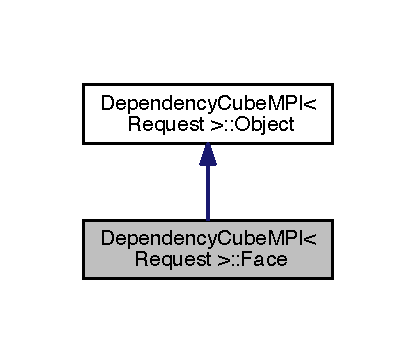
\includegraphics[width=200pt]{dd/dee/struct_dependency_cube_m_p_i_1_1_face__inherit__graph}
\end{center}
\end{figure}


Collaboration diagram for Dependency\+Cube\+M\+P\+I$<$ Request $>$\+:\+:Face\+:\nopagebreak
\begin{figure}[H]
\begin{center}
\leavevmode
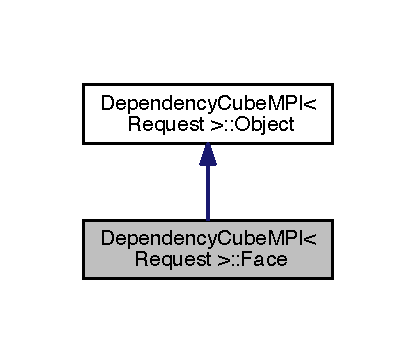
\includegraphics[width=200pt]{d9/de6/struct_dependency_cube_m_p_i_1_1_face__coll__graph}
\end{center}
\end{figure}
\subsection*{Public Member Functions}
\begin{DoxyCompactItemize}
\item 
\hyperlink{struct_dependency_cube_m_p_i_1_1_face_a6fdbbfc5d6d27acbc0765c03aed7606a}{Face} ()
\item 
\hyperlink{struct_dependency_cube_m_p_i_1_1_face_a23f82a7099e13def1a59b4d40c1da674}{Face} (Direction \hyperlink{struct_dependency_cube_m_p_i_1_1_face_a8ca1f274c00b7e97ab3c327d3236494f}{d}, Side \hyperlink{struct_dependency_cube_m_p_i_1_1_face_a0f93c85a3376303880fc199236b0e3da}{s})
\item 
\hyperlink{struct_dependency_cube_m_p_i_1_1_face}{Face} \& \hyperlink{struct_dependency_cube_m_p_i_1_1_face_abdc8f00313364053f6756d6df3d24d80}{operator=} (const \hyperlink{struct_dependency_cube_m_p_i_1_1_face}{Face} \&f)
\item 
\hyperlink{struct_region}{Region} \hyperlink{struct_dependency_cube_m_p_i_1_1_face_aac6960e98b8018d962de087d4052fa6f}{get\+Region} (const int n\mbox{[}3\mbox{]})
\end{DoxyCompactItemize}
\subsection*{Public Attributes}
\begin{DoxyCompactItemize}
\item 
Direction \hyperlink{struct_dependency_cube_m_p_i_1_1_face_a8ca1f274c00b7e97ab3c327d3236494f}{d}
\item 
Side \hyperlink{struct_dependency_cube_m_p_i_1_1_face_a0f93c85a3376303880fc199236b0e3da}{s}
\end{DoxyCompactItemize}


\subsection{Constructor \& Destructor Documentation}
\hypertarget{struct_dependency_cube_m_p_i_1_1_face_a6fdbbfc5d6d27acbc0765c03aed7606a}{}\index{Dependency\+Cube\+M\+P\+I\+::\+Face@{Dependency\+Cube\+M\+P\+I\+::\+Face}!Face@{Face}}
\index{Face@{Face}!Dependency\+Cube\+M\+P\+I\+::\+Face@{Dependency\+Cube\+M\+P\+I\+::\+Face}}
\subsubsection[{Face}]{\setlength{\rightskip}{0pt plus 5cm}template$<$typename Request$>$ {\bf Dependency\+Cube\+M\+P\+I}$<$ Request $>$\+::Face\+::\+Face (
\begin{DoxyParamCaption}
{}
\end{DoxyParamCaption}
)\hspace{0.3cm}{\ttfamily [inline]}}\label{struct_dependency_cube_m_p_i_1_1_face_a6fdbbfc5d6d27acbc0765c03aed7606a}
\hypertarget{struct_dependency_cube_m_p_i_1_1_face_a23f82a7099e13def1a59b4d40c1da674}{}\index{Dependency\+Cube\+M\+P\+I\+::\+Face@{Dependency\+Cube\+M\+P\+I\+::\+Face}!Face@{Face}}
\index{Face@{Face}!Dependency\+Cube\+M\+P\+I\+::\+Face@{Dependency\+Cube\+M\+P\+I\+::\+Face}}
\subsubsection[{Face}]{\setlength{\rightskip}{0pt plus 5cm}template$<$typename Request$>$ {\bf Dependency\+Cube\+M\+P\+I}$<$ Request $>$\+::Face\+::\+Face (
\begin{DoxyParamCaption}
\item[{Direction}]{d, }
\item[{Side}]{s}
\end{DoxyParamCaption}
)\hspace{0.3cm}{\ttfamily [inline]}}\label{struct_dependency_cube_m_p_i_1_1_face_a23f82a7099e13def1a59b4d40c1da674}


\subsection{Member Function Documentation}
\hypertarget{struct_dependency_cube_m_p_i_1_1_face_aac6960e98b8018d962de087d4052fa6f}{}\index{Dependency\+Cube\+M\+P\+I\+::\+Face@{Dependency\+Cube\+M\+P\+I\+::\+Face}!get\+Region@{get\+Region}}
\index{get\+Region@{get\+Region}!Dependency\+Cube\+M\+P\+I\+::\+Face@{Dependency\+Cube\+M\+P\+I\+::\+Face}}
\subsubsection[{get\+Region}]{\setlength{\rightskip}{0pt plus 5cm}template$<$typename Request$>$ {\bf Region} {\bf Dependency\+Cube\+M\+P\+I}$<$ Request $>$\+::Face\+::get\+Region (
\begin{DoxyParamCaption}
\item[{const int}]{n\mbox{[}3\mbox{]}}
\end{DoxyParamCaption}
)\hspace{0.3cm}{\ttfamily [inline]}}\label{struct_dependency_cube_m_p_i_1_1_face_aac6960e98b8018d962de087d4052fa6f}
\hypertarget{struct_dependency_cube_m_p_i_1_1_face_abdc8f00313364053f6756d6df3d24d80}{}\index{Dependency\+Cube\+M\+P\+I\+::\+Face@{Dependency\+Cube\+M\+P\+I\+::\+Face}!operator=@{operator=}}
\index{operator=@{operator=}!Dependency\+Cube\+M\+P\+I\+::\+Face@{Dependency\+Cube\+M\+P\+I\+::\+Face}}
\subsubsection[{operator=}]{\setlength{\rightskip}{0pt plus 5cm}template$<$typename Request$>$ {\bf Face}\& {\bf Dependency\+Cube\+M\+P\+I}$<$ Request $>$\+::Face\+::operator= (
\begin{DoxyParamCaption}
\item[{const {\bf Face} \&}]{f}
\end{DoxyParamCaption}
)\hspace{0.3cm}{\ttfamily [inline]}}\label{struct_dependency_cube_m_p_i_1_1_face_abdc8f00313364053f6756d6df3d24d80}


\subsection{Member Data Documentation}
\hypertarget{struct_dependency_cube_m_p_i_1_1_face_a8ca1f274c00b7e97ab3c327d3236494f}{}\index{Dependency\+Cube\+M\+P\+I\+::\+Face@{Dependency\+Cube\+M\+P\+I\+::\+Face}!d@{d}}
\index{d@{d}!Dependency\+Cube\+M\+P\+I\+::\+Face@{Dependency\+Cube\+M\+P\+I\+::\+Face}}
\subsubsection[{d}]{\setlength{\rightskip}{0pt plus 5cm}template$<$typename Request$>$ Direction {\bf Dependency\+Cube\+M\+P\+I}$<$ Request $>$\+::Face\+::d}\label{struct_dependency_cube_m_p_i_1_1_face_a8ca1f274c00b7e97ab3c327d3236494f}
\hypertarget{struct_dependency_cube_m_p_i_1_1_face_a0f93c85a3376303880fc199236b0e3da}{}\index{Dependency\+Cube\+M\+P\+I\+::\+Face@{Dependency\+Cube\+M\+P\+I\+::\+Face}!s@{s}}
\index{s@{s}!Dependency\+Cube\+M\+P\+I\+::\+Face@{Dependency\+Cube\+M\+P\+I\+::\+Face}}
\subsubsection[{s}]{\setlength{\rightskip}{0pt plus 5cm}template$<$typename Request$>$ Side {\bf Dependency\+Cube\+M\+P\+I}$<$ Request $>$\+::Face\+::s}\label{struct_dependency_cube_m_p_i_1_1_face_a0f93c85a3376303880fc199236b0e3da}


The documentation for this struct was generated from the following file\+:\begin{DoxyCompactItemize}
\item 
Cubism/\hyperlink{_dependency_cube_m_p_i_8h}{Dependency\+Cube\+M\+P\+I.\+h}\end{DoxyCompactItemize}

\hypertarget{struct_f_f_t_w___i_n_i_t}{}\section{F\+F\+T\+W\+\_\+\+I\+N\+I\+T$<$ T $>$ Struct Template Reference}
\label{struct_f_f_t_w___i_n_i_t}\index{F\+F\+T\+W\+\_\+\+I\+N\+I\+T$<$ T $>$@{F\+F\+T\+W\+\_\+\+I\+N\+I\+T$<$ T $>$}}


{\ttfamily \#include $<$Operators\+\_\+\+D\+F\+T.\+h$>$}



The documentation for this struct was generated from the following file\+:\begin{DoxyCompactItemize}
\item 
/\+Users/cconti/\+Desktop/\+Mounts/\+Brutus\+Home/\+Seed/\+Cubism\+U\+P\+\_\+2\+D/source/\hyperlink{_operators___d_f_t_8h}{Operators\+\_\+\+D\+F\+T.\+h}\end{DoxyCompactItemize}

\hypertarget{struct_f_f_t_w___i_n_i_t_3_01double_01_4}{}\section{F\+F\+T\+W\+\_\+\+I\+N\+I\+T$<$ double $>$ Struct Template Reference}
\label{struct_f_f_t_w___i_n_i_t_3_01double_01_4}\index{F\+F\+T\+W\+\_\+\+I\+N\+I\+T$<$ double $>$@{F\+F\+T\+W\+\_\+\+I\+N\+I\+T$<$ double $>$}}


{\ttfamily \#include $<$Operators\+\_\+\+D\+F\+T.\+h$>$}

\subsection*{Public Member Functions}
\begin{DoxyCompactItemize}
\item 
\hyperlink{struct_f_f_t_w___i_n_i_t_3_01double_01_4_ac70ec8b65ae3324527d4ee308ee7a7bd}{F\+F\+T\+W\+\_\+\+I\+N\+I\+T} ()
\end{DoxyCompactItemize}


\subsection{Constructor \& Destructor Documentation}
\hypertarget{struct_f_f_t_w___i_n_i_t_3_01double_01_4_ac70ec8b65ae3324527d4ee308ee7a7bd}{}\index{F\+F\+T\+W\+\_\+\+I\+N\+I\+T$<$ double $>$@{F\+F\+T\+W\+\_\+\+I\+N\+I\+T$<$ double $>$}!F\+F\+T\+W\+\_\+\+I\+N\+I\+T@{F\+F\+T\+W\+\_\+\+I\+N\+I\+T}}
\index{F\+F\+T\+W\+\_\+\+I\+N\+I\+T@{F\+F\+T\+W\+\_\+\+I\+N\+I\+T}!F\+F\+T\+W\+\_\+\+I\+N\+I\+T$<$ double $>$@{F\+F\+T\+W\+\_\+\+I\+N\+I\+T$<$ double $>$}}
\subsubsection[{F\+F\+T\+W\+\_\+\+I\+N\+I\+T}]{\setlength{\rightskip}{0pt plus 5cm}{\bf F\+F\+T\+W\+\_\+\+I\+N\+I\+T}$<$ double $>$\+::{\bf F\+F\+T\+W\+\_\+\+I\+N\+I\+T} (
\begin{DoxyParamCaption}
{}
\end{DoxyParamCaption}
)\hspace{0.3cm}{\ttfamily [inline]}}\label{struct_f_f_t_w___i_n_i_t_3_01double_01_4_ac70ec8b65ae3324527d4ee308ee7a7bd}


Here is the call graph for this function\+:
% FIG 0




Here is the caller graph for this function\+:
% FIG 1




The documentation for this struct was generated from the following file\+:\begin{DoxyCompactItemize}
\item 
/\+Users/cconti/\+Desktop/\+Mounts/\+Brutus\+Home/\+Seed/\+Cubism\+U\+P\+\_\+2\+D/source/\hyperlink{_operators___d_f_t_8h}{Operators\+\_\+\+D\+F\+T.\+h}\end{DoxyCompactItemize}

\hypertarget{struct_f_f_t_w___i_n_i_t_3_01float_01_4}{}\section{F\+F\+T\+W\+\_\+\+I\+N\+I\+T$<$ float $>$ Struct Template Reference}
\label{struct_f_f_t_w___i_n_i_t_3_01float_01_4}\index{F\+F\+T\+W\+\_\+\+I\+N\+I\+T$<$ float $>$@{F\+F\+T\+W\+\_\+\+I\+N\+I\+T$<$ float $>$}}


{\ttfamily \#include $<$Operators\+\_\+\+D\+F\+T.\+h$>$}

\subsection*{Public Member Functions}
\begin{DoxyCompactItemize}
\item 
\hyperlink{struct_f_f_t_w___i_n_i_t_3_01float_01_4_a95bf95941156ade33f2d8c8b7bda2e02}{F\+F\+T\+W\+\_\+\+I\+N\+I\+T} ()
\end{DoxyCompactItemize}


\subsection{Constructor \& Destructor Documentation}
\hypertarget{struct_f_f_t_w___i_n_i_t_3_01float_01_4_a95bf95941156ade33f2d8c8b7bda2e02}{}\index{F\+F\+T\+W\+\_\+\+I\+N\+I\+T$<$ float $>$@{F\+F\+T\+W\+\_\+\+I\+N\+I\+T$<$ float $>$}!F\+F\+T\+W\+\_\+\+I\+N\+I\+T@{F\+F\+T\+W\+\_\+\+I\+N\+I\+T}}
\index{F\+F\+T\+W\+\_\+\+I\+N\+I\+T@{F\+F\+T\+W\+\_\+\+I\+N\+I\+T}!F\+F\+T\+W\+\_\+\+I\+N\+I\+T$<$ float $>$@{F\+F\+T\+W\+\_\+\+I\+N\+I\+T$<$ float $>$}}
\subsubsection[{F\+F\+T\+W\+\_\+\+I\+N\+I\+T}]{\setlength{\rightskip}{0pt plus 5cm}{\bf F\+F\+T\+W\+\_\+\+I\+N\+I\+T}$<$ float $>$\+::{\bf F\+F\+T\+W\+\_\+\+I\+N\+I\+T} (
\begin{DoxyParamCaption}
{}
\end{DoxyParamCaption}
)\hspace{0.3cm}{\ttfamily [inline]}}\label{struct_f_f_t_w___i_n_i_t_3_01float_01_4_a95bf95941156ade33f2d8c8b7bda2e02}


Here is the call graph for this function\+:\nopagebreak
\begin{figure}[H]
\begin{center}
\leavevmode
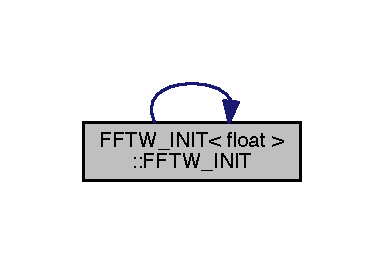
\includegraphics[width=184pt]{d2/de1/struct_f_f_t_w___i_n_i_t_3_01float_01_4_a95bf95941156ade33f2d8c8b7bda2e02_cgraph}
\end{center}
\end{figure}




Here is the caller graph for this function\+:\nopagebreak
\begin{figure}[H]
\begin{center}
\leavevmode
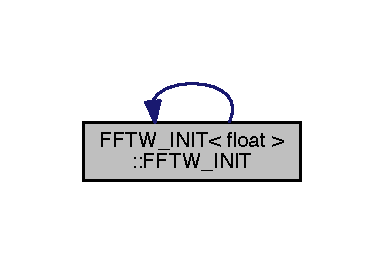
\includegraphics[width=184pt]{d2/de1/struct_f_f_t_w___i_n_i_t_3_01float_01_4_a95bf95941156ade33f2d8c8b7bda2e02_icgraph}
\end{center}
\end{figure}




The documentation for this struct was generated from the following file\+:\begin{DoxyCompactItemize}
\item 
source/\hyperlink{_operators___d_f_t_8h}{Operators\+\_\+\+D\+F\+T.\+h}\end{DoxyCompactItemize}

\hypertarget{struct_f_f_t_w___t_y_p_e_s}{}\section{F\+F\+T\+W\+\_\+\+T\+Y\+P\+E\+S$<$ T $>$ Struct Template Reference}
\label{struct_f_f_t_w___t_y_p_e_s}\index{F\+F\+T\+W\+\_\+\+T\+Y\+P\+E\+S$<$ T $>$@{F\+F\+T\+W\+\_\+\+T\+Y\+P\+E\+S$<$ T $>$}}


{\ttfamily \#include $<$Operators\+\_\+\+D\+F\+T.\+h$>$}



The documentation for this struct was generated from the following file\+:\begin{DoxyCompactItemize}
\item 
/\+Users/cconti/\+Desktop/\+Mounts/\+Brutus\+Home/\+Cubism\+U\+P\+\_\+2\+D/source/\hyperlink{_operators___d_f_t_8h}{Operators\+\_\+\+D\+F\+T.\+h}\end{DoxyCompactItemize}

\hypertarget{struct_f_f_t_w___t_y_p_e_s_3_01double_01_4}{}\section{F\+F\+T\+W\+\_\+\+T\+Y\+P\+E\+S$<$ double $>$ Struct Template Reference}
\label{struct_f_f_t_w___t_y_p_e_s_3_01double_01_4}\index{F\+F\+T\+W\+\_\+\+T\+Y\+P\+E\+S$<$ double $>$@{F\+F\+T\+W\+\_\+\+T\+Y\+P\+E\+S$<$ double $>$}}


{\ttfamily \#include $<$Operators\+\_\+\+D\+F\+T.\+h$>$}

\subsection*{Classes}
\begin{DoxyCompactItemize}
\item 
struct \hyperlink{struct_f_f_t_w___t_y_p_e_s_3_01double_01_4_1_1_a_l_l_o_c_a_t_o_r}{A\+L\+L\+O\+C\+A\+T\+O\+R}
\item 
struct \hyperlink{struct_f_f_t_w___t_y_p_e_s_3_01double_01_4_1_1_p_l_a_n_n_e_r}{P\+L\+A\+N\+N\+E\+R}
\end{DoxyCompactItemize}
\subsection*{Public Types}
\begin{DoxyCompactItemize}
\item 
typedef fftw\+\_\+complex \hyperlink{struct_f_f_t_w___t_y_p_e_s_3_01double_01_4_a9e1b7d8a842e1afab769065e5873f78c}{C\+O\+M\+P\+L\+E\+X}
\item 
typedef fftw\+\_\+plan \hyperlink{struct_f_f_t_w___t_y_p_e_s_3_01double_01_4_a19c1538d166a5a9f01680c00253850ac}{P\+L\+A\+N}
\end{DoxyCompactItemize}


\subsection{Member Typedef Documentation}
\hypertarget{struct_f_f_t_w___t_y_p_e_s_3_01double_01_4_a9e1b7d8a842e1afab769065e5873f78c}{}\index{F\+F\+T\+W\+\_\+\+T\+Y\+P\+E\+S$<$ double $>$@{F\+F\+T\+W\+\_\+\+T\+Y\+P\+E\+S$<$ double $>$}!C\+O\+M\+P\+L\+E\+X@{C\+O\+M\+P\+L\+E\+X}}
\index{C\+O\+M\+P\+L\+E\+X@{C\+O\+M\+P\+L\+E\+X}!F\+F\+T\+W\+\_\+\+T\+Y\+P\+E\+S$<$ double $>$@{F\+F\+T\+W\+\_\+\+T\+Y\+P\+E\+S$<$ double $>$}}
\subsubsection[{C\+O\+M\+P\+L\+E\+X}]{\setlength{\rightskip}{0pt plus 5cm}typedef fftw\+\_\+complex {\bf F\+F\+T\+W\+\_\+\+T\+Y\+P\+E\+S}$<$ double $>$\+::{\bf C\+O\+M\+P\+L\+E\+X}}\label{struct_f_f_t_w___t_y_p_e_s_3_01double_01_4_a9e1b7d8a842e1afab769065e5873f78c}
\hypertarget{struct_f_f_t_w___t_y_p_e_s_3_01double_01_4_a19c1538d166a5a9f01680c00253850ac}{}\index{F\+F\+T\+W\+\_\+\+T\+Y\+P\+E\+S$<$ double $>$@{F\+F\+T\+W\+\_\+\+T\+Y\+P\+E\+S$<$ double $>$}!P\+L\+A\+N@{P\+L\+A\+N}}
\index{P\+L\+A\+N@{P\+L\+A\+N}!F\+F\+T\+W\+\_\+\+T\+Y\+P\+E\+S$<$ double $>$@{F\+F\+T\+W\+\_\+\+T\+Y\+P\+E\+S$<$ double $>$}}
\subsubsection[{P\+L\+A\+N}]{\setlength{\rightskip}{0pt plus 5cm}typedef fftw\+\_\+plan {\bf F\+F\+T\+W\+\_\+\+T\+Y\+P\+E\+S}$<$ double $>$\+::{\bf P\+L\+A\+N}}\label{struct_f_f_t_w___t_y_p_e_s_3_01double_01_4_a19c1538d166a5a9f01680c00253850ac}


The documentation for this struct was generated from the following file\+:\begin{DoxyCompactItemize}
\item 
/\+Users/cconti/\+Desktop/\+Mounts/\+Brutus\+Home/\+Cubism\+U\+P\+\_\+2\+D/source/\hyperlink{_operators___d_f_t_8h}{Operators\+\_\+\+D\+F\+T.\+h}\end{DoxyCompactItemize}

\hypertarget{struct_f_f_t_w___t_y_p_e_s_3_01float_01_4}{}\section{F\+F\+T\+W\+\_\+\+T\+Y\+P\+E\+S$<$ float $>$ Struct Template Reference}
\label{struct_f_f_t_w___t_y_p_e_s_3_01float_01_4}\index{F\+F\+T\+W\+\_\+\+T\+Y\+P\+E\+S$<$ float $>$@{F\+F\+T\+W\+\_\+\+T\+Y\+P\+E\+S$<$ float $>$}}


{\ttfamily \#include $<$Operators\+\_\+\+D\+F\+T.\+h$>$}

\subsection*{Classes}
\begin{DoxyCompactItemize}
\item 
struct \hyperlink{struct_f_f_t_w___t_y_p_e_s_3_01float_01_4_1_1_a_l_l_o_c_a_t_o_r}{A\+L\+L\+O\+C\+A\+T\+O\+R}
\item 
struct \hyperlink{struct_f_f_t_w___t_y_p_e_s_3_01float_01_4_1_1_p_l_a_n_n_e_r}{P\+L\+A\+N\+N\+E\+R}
\end{DoxyCompactItemize}
\subsection*{Public Types}
\begin{DoxyCompactItemize}
\item 
typedef fftwf\+\_\+complex \hyperlink{struct_f_f_t_w___t_y_p_e_s_3_01float_01_4_a0039a21dbbd01522d970667b3480a169}{C\+O\+M\+P\+L\+E\+X}
\item 
typedef fftwf\+\_\+plan \hyperlink{struct_f_f_t_w___t_y_p_e_s_3_01float_01_4_a564fe6a699a8574500c81d7d43b23980}{P\+L\+A\+N}
\end{DoxyCompactItemize}


\subsection{Member Typedef Documentation}
\hypertarget{struct_f_f_t_w___t_y_p_e_s_3_01float_01_4_a0039a21dbbd01522d970667b3480a169}{}\index{F\+F\+T\+W\+\_\+\+T\+Y\+P\+E\+S$<$ float $>$@{F\+F\+T\+W\+\_\+\+T\+Y\+P\+E\+S$<$ float $>$}!C\+O\+M\+P\+L\+E\+X@{C\+O\+M\+P\+L\+E\+X}}
\index{C\+O\+M\+P\+L\+E\+X@{C\+O\+M\+P\+L\+E\+X}!F\+F\+T\+W\+\_\+\+T\+Y\+P\+E\+S$<$ float $>$@{F\+F\+T\+W\+\_\+\+T\+Y\+P\+E\+S$<$ float $>$}}
\subsubsection[{C\+O\+M\+P\+L\+E\+X}]{\setlength{\rightskip}{0pt plus 5cm}typedef fftwf\+\_\+complex {\bf F\+F\+T\+W\+\_\+\+T\+Y\+P\+E\+S}$<$ float $>$\+::{\bf C\+O\+M\+P\+L\+E\+X}}\label{struct_f_f_t_w___t_y_p_e_s_3_01float_01_4_a0039a21dbbd01522d970667b3480a169}
\hypertarget{struct_f_f_t_w___t_y_p_e_s_3_01float_01_4_a564fe6a699a8574500c81d7d43b23980}{}\index{F\+F\+T\+W\+\_\+\+T\+Y\+P\+E\+S$<$ float $>$@{F\+F\+T\+W\+\_\+\+T\+Y\+P\+E\+S$<$ float $>$}!P\+L\+A\+N@{P\+L\+A\+N}}
\index{P\+L\+A\+N@{P\+L\+A\+N}!F\+F\+T\+W\+\_\+\+T\+Y\+P\+E\+S$<$ float $>$@{F\+F\+T\+W\+\_\+\+T\+Y\+P\+E\+S$<$ float $>$}}
\subsubsection[{P\+L\+A\+N}]{\setlength{\rightskip}{0pt plus 5cm}typedef fftwf\+\_\+plan {\bf F\+F\+T\+W\+\_\+\+T\+Y\+P\+E\+S}$<$ float $>$\+::{\bf P\+L\+A\+N}}\label{struct_f_f_t_w___t_y_p_e_s_3_01float_01_4_a564fe6a699a8574500c81d7d43b23980}


The documentation for this struct was generated from the following file\+:\begin{DoxyCompactItemize}
\item 
/\+Users/cconti/\+Desktop/\+Mounts/\+Brutus\+Home/\+Seed/\+Cubism\+U\+P\+\_\+2\+D/source/\hyperlink{_operators___d_f_t_8h}{Operators\+\_\+\+D\+F\+T.\+h}\end{DoxyCompactItemize}

\hypertarget{class_f_f_t_w_base}{}\section{F\+F\+T\+W\+Base Class Reference}
\label{class_f_f_t_w_base}\index{F\+F\+T\+W\+Base@{F\+F\+T\+W\+Base}}


{\ttfamily \#include $<$Poisson\+Solver\+Scalar\+F\+F\+T\+W.\+h$>$}



Inheritance diagram for F\+F\+T\+W\+Base\+:\nopagebreak
\begin{figure}[H]
\begin{center}
\leavevmode
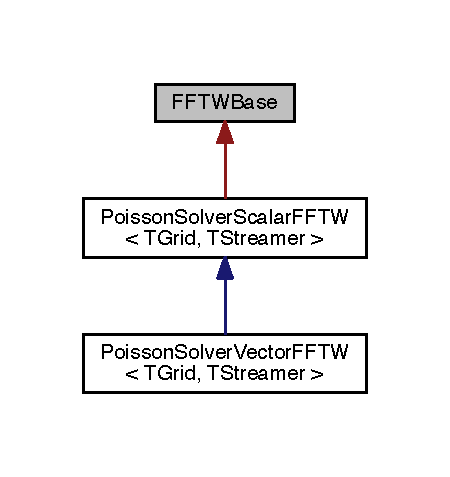
\includegraphics[width=216pt]{d3/d08/class_f_f_t_w_base__inherit__graph}
\end{center}
\end{figure}
\subsection*{Public Member Functions}
\begin{DoxyCompactItemize}
\item 
\hyperlink{class_f_f_t_w_base_ad4184aa852af23c642e39f69d98ce196}{F\+F\+T\+W\+Base} (const int desired\+\_\+threads)
\end{DoxyCompactItemize}
\subsection*{Static Public Member Functions}
\begin{DoxyCompactItemize}
\item 
static void \hyperlink{class_f_f_t_w_base_a4258f11b605bb1e3f0679f020a73aa18}{dispose} ()
\end{DoxyCompactItemize}


\subsection{Constructor \& Destructor Documentation}
\hypertarget{class_f_f_t_w_base_ad4184aa852af23c642e39f69d98ce196}{}\index{F\+F\+T\+W\+Base@{F\+F\+T\+W\+Base}!F\+F\+T\+W\+Base@{F\+F\+T\+W\+Base}}
\index{F\+F\+T\+W\+Base@{F\+F\+T\+W\+Base}!F\+F\+T\+W\+Base@{F\+F\+T\+W\+Base}}
\subsubsection[{F\+F\+T\+W\+Base}]{\setlength{\rightskip}{0pt plus 5cm}F\+F\+T\+W\+Base\+::\+F\+F\+T\+W\+Base (
\begin{DoxyParamCaption}
\item[{const int}]{desired\+\_\+threads}
\end{DoxyParamCaption}
)\hspace{0.3cm}{\ttfamily [inline]}}\label{class_f_f_t_w_base_ad4184aa852af23c642e39f69d98ce196}


\subsection{Member Function Documentation}
\hypertarget{class_f_f_t_w_base_a4258f11b605bb1e3f0679f020a73aa18}{}\index{F\+F\+T\+W\+Base@{F\+F\+T\+W\+Base}!dispose@{dispose}}
\index{dispose@{dispose}!F\+F\+T\+W\+Base@{F\+F\+T\+W\+Base}}
\subsubsection[{dispose}]{\setlength{\rightskip}{0pt plus 5cm}static void F\+F\+T\+W\+Base\+::dispose (
\begin{DoxyParamCaption}
{}
\end{DoxyParamCaption}
)\hspace{0.3cm}{\ttfamily [inline]}, {\ttfamily [static]}}\label{class_f_f_t_w_base_a4258f11b605bb1e3f0679f020a73aa18}


Here is the caller graph for this function\+:\nopagebreak
\begin{figure}[H]
\begin{center}
\leavevmode
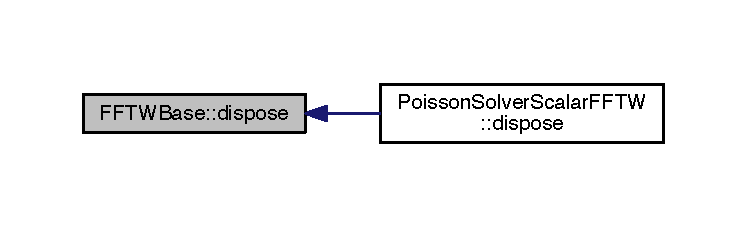
\includegraphics[width=350pt]{d3/d51/class_f_f_t_w_base_a4258f11b605bb1e3f0679f020a73aa18_icgraph}
\end{center}
\end{figure}




The documentation for this class was generated from the following files\+:\begin{DoxyCompactItemize}
\item 
source/\hyperlink{_poisson_solver_scalar_f_f_t_w_8h}{Poisson\+Solver\+Scalar\+F\+F\+T\+W.\+h}\item 
source/\hyperlink{_poisson_solver_scalar_f_f_t_w_8cpp}{Poisson\+Solver\+Scalar\+F\+F\+T\+W.\+cpp}\end{DoxyCompactItemize}

\hypertarget{struct_fluid_block}{}\section{Fluid\+Block Struct Reference}
\label{struct_fluid_block}\index{Fluid\+Block@{Fluid\+Block}}


{\ttfamily \#include $<$Definitions.\+h$>$}



Collaboration diagram for Fluid\+Block\+:\nopagebreak
\begin{figure}[H]
\begin{center}
\leavevmode
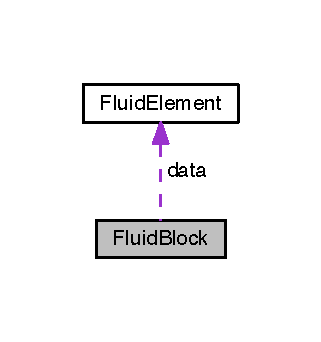
\includegraphics[width=154pt]{d1/da0/struct_fluid_block__coll__graph}
\end{center}
\end{figure}
\subsection*{Public Types}
\begin{DoxyCompactItemize}
\item 
typedef \hyperlink{struct_fluid_element}{Fluid\+Element} \hyperlink{struct_fluid_block_ada33fbdab33f2688d3eb632118de5a6e}{Element\+Type}
\end{DoxyCompactItemize}
\subsection*{Public Member Functions}
\begin{DoxyCompactItemize}
\item 
void \hyperlink{struct_fluid_block_af2c2703f49640b00d0757ab6d22bdec9}{clear} ()
\item 
\hyperlink{struct_fluid_element}{Fluid\+Element} \& \hyperlink{struct_fluid_block_a0cc6dc89e9a9a3b9c1b61eda26a041eb}{operator()} (int ix, int iy=0, int iz=0)
\item 
{\footnotesize template$<$typename Streamer $>$ }\\void \hyperlink{struct_fluid_block_a1737418d1510f3ac1ab6750c9738568d}{Write} (ofstream \&output, Streamer streamer) const 
\item 
{\footnotesize template$<$typename Streamer $>$ }\\void \hyperlink{struct_fluid_block_a903987108c4851693bc498a736010aff}{Read} (ifstream \&input, Streamer streamer)
\item 
{\footnotesize template$<$$>$ }\\void \hyperlink{struct_fluid_block_a30bcb9d7e2f10a1e27c3eb2898c02981}{Write} (ofstream \&output, \hyperlink{struct_streamer_grid_point}{Streamer\+Grid\+Point} streamer) const 
\item 
{\footnotesize template$<$$>$ }\\void \hyperlink{struct_fluid_block_ab68e1e1b161ea573e9b8adda1538ae0c}{Read} (ifstream \&input, \hyperlink{struct_streamer_grid_point}{Streamer\+Grid\+Point} streamer)
\end{DoxyCompactItemize}
\subsection*{Public Attributes}
\begin{DoxyCompactItemize}
\item 
\hyperlink{struct_fluid_element}{Fluid\+Element} \hyperlink{struct_fluid_block_adaf63688f4901ef6640e3ee02aeabf42}{data} \mbox{[}1\mbox{]}\mbox{[}\hyperlink{struct_fluid_block_afd21ed464f6732be798bba7d87113bd2}{size\+Y}\mbox{]}\mbox{[}\hyperlink{struct_fluid_block_a4894f513519efdad2837a01cfb65f42e}{size\+X}\mbox{]}
\end{DoxyCompactItemize}
\subsection*{Static Public Attributes}
\begin{DoxyCompactItemize}
\item 
static const int \hyperlink{struct_fluid_block_a4894f513519efdad2837a01cfb65f42e}{size\+X} = \hyperlink{_definitions_8h_a6a273e4b23a982a4fcd5b26ab5a20888}{\+\_\+\+B\+S\+\_\+}
\item 
static const int \hyperlink{struct_fluid_block_afd21ed464f6732be798bba7d87113bd2}{size\+Y} = \hyperlink{_definitions_8h_a6a273e4b23a982a4fcd5b26ab5a20888}{\+\_\+\+B\+S\+\_\+}
\item 
static const int \hyperlink{struct_fluid_block_a7876602d8791ed7d4734fa20ad0a9574}{size\+Z} = 1
\end{DoxyCompactItemize}


\subsection{Member Typedef Documentation}
\hypertarget{struct_fluid_block_ada33fbdab33f2688d3eb632118de5a6e}{}\index{Fluid\+Block@{Fluid\+Block}!Element\+Type@{Element\+Type}}
\index{Element\+Type@{Element\+Type}!Fluid\+Block@{Fluid\+Block}}
\subsubsection[{Element\+Type}]{\setlength{\rightskip}{0pt plus 5cm}typedef {\bf Fluid\+Element} {\bf Fluid\+Block\+::\+Element\+Type}}\label{struct_fluid_block_ada33fbdab33f2688d3eb632118de5a6e}


\subsection{Member Function Documentation}
\hypertarget{struct_fluid_block_af2c2703f49640b00d0757ab6d22bdec9}{}\index{Fluid\+Block@{Fluid\+Block}!clear@{clear}}
\index{clear@{clear}!Fluid\+Block@{Fluid\+Block}}
\subsubsection[{clear}]{\setlength{\rightskip}{0pt plus 5cm}void Fluid\+Block\+::clear (
\begin{DoxyParamCaption}
{}
\end{DoxyParamCaption}
)\hspace{0.3cm}{\ttfamily [inline]}}\label{struct_fluid_block_af2c2703f49640b00d0757ab6d22bdec9}
\hypertarget{struct_fluid_block_a0cc6dc89e9a9a3b9c1b61eda26a041eb}{}\index{Fluid\+Block@{Fluid\+Block}!operator()@{operator()}}
\index{operator()@{operator()}!Fluid\+Block@{Fluid\+Block}}
\subsubsection[{operator()}]{\setlength{\rightskip}{0pt plus 5cm}{\bf Fluid\+Element}\& Fluid\+Block\+::operator() (
\begin{DoxyParamCaption}
\item[{int}]{ix, }
\item[{int}]{iy = {\ttfamily 0}, }
\item[{int}]{iz = {\ttfamily 0}}
\end{DoxyParamCaption}
)\hspace{0.3cm}{\ttfamily [inline]}}\label{struct_fluid_block_a0cc6dc89e9a9a3b9c1b61eda26a041eb}
\hypertarget{struct_fluid_block_a903987108c4851693bc498a736010aff}{}\index{Fluid\+Block@{Fluid\+Block}!Read@{Read}}
\index{Read@{Read}!Fluid\+Block@{Fluid\+Block}}
\subsubsection[{Read}]{\setlength{\rightskip}{0pt plus 5cm}template$<$typename Streamer $>$ void Fluid\+Block\+::\+Read (
\begin{DoxyParamCaption}
\item[{ifstream \&}]{input, }
\item[{Streamer}]{streamer}
\end{DoxyParamCaption}
)\hspace{0.3cm}{\ttfamily [inline]}}\label{struct_fluid_block_a903987108c4851693bc498a736010aff}
\hypertarget{struct_fluid_block_ab68e1e1b161ea573e9b8adda1538ae0c}{}\index{Fluid\+Block@{Fluid\+Block}!Read@{Read}}
\index{Read@{Read}!Fluid\+Block@{Fluid\+Block}}
\subsubsection[{Read}]{\setlength{\rightskip}{0pt plus 5cm}template$<$$>$ void Fluid\+Block\+::\+Read (
\begin{DoxyParamCaption}
\item[{ifstream \&}]{input, }
\item[{{\bf Streamer\+Grid\+Point}}]{streamer}
\end{DoxyParamCaption}
)\hspace{0.3cm}{\ttfamily [inline]}}\label{struct_fluid_block_ab68e1e1b161ea573e9b8adda1538ae0c}
\hypertarget{struct_fluid_block_a1737418d1510f3ac1ab6750c9738568d}{}\index{Fluid\+Block@{Fluid\+Block}!Write@{Write}}
\index{Write@{Write}!Fluid\+Block@{Fluid\+Block}}
\subsubsection[{Write}]{\setlength{\rightskip}{0pt plus 5cm}template$<$typename Streamer $>$ void Fluid\+Block\+::\+Write (
\begin{DoxyParamCaption}
\item[{ofstream \&}]{output, }
\item[{Streamer}]{streamer}
\end{DoxyParamCaption}
) const\hspace{0.3cm}{\ttfamily [inline]}}\label{struct_fluid_block_a1737418d1510f3ac1ab6750c9738568d}
\hypertarget{struct_fluid_block_a30bcb9d7e2f10a1e27c3eb2898c02981}{}\index{Fluid\+Block@{Fluid\+Block}!Write@{Write}}
\index{Write@{Write}!Fluid\+Block@{Fluid\+Block}}
\subsubsection[{Write}]{\setlength{\rightskip}{0pt plus 5cm}template$<$$>$ void Fluid\+Block\+::\+Write (
\begin{DoxyParamCaption}
\item[{ofstream \&}]{output, }
\item[{{\bf Streamer\+Grid\+Point}}]{streamer}
\end{DoxyParamCaption}
) const\hspace{0.3cm}{\ttfamily [inline]}}\label{struct_fluid_block_a30bcb9d7e2f10a1e27c3eb2898c02981}


\subsection{Member Data Documentation}
\hypertarget{struct_fluid_block_adaf63688f4901ef6640e3ee02aeabf42}{}\index{Fluid\+Block@{Fluid\+Block}!data@{data}}
\index{data@{data}!Fluid\+Block@{Fluid\+Block}}
\subsubsection[{data}]{\setlength{\rightskip}{0pt plus 5cm}{\bf Fluid\+Element} Fluid\+Block\+::data\mbox{[}1\mbox{]}\mbox{[}{\bf size\+Y}\mbox{]}\mbox{[}{\bf size\+X}\mbox{]}}\label{struct_fluid_block_adaf63688f4901ef6640e3ee02aeabf42}
\hypertarget{struct_fluid_block_a4894f513519efdad2837a01cfb65f42e}{}\index{Fluid\+Block@{Fluid\+Block}!size\+X@{size\+X}}
\index{size\+X@{size\+X}!Fluid\+Block@{Fluid\+Block}}
\subsubsection[{size\+X}]{\setlength{\rightskip}{0pt plus 5cm}const int Fluid\+Block\+::size\+X = {\bf \+\_\+\+B\+S\+\_\+}\hspace{0.3cm}{\ttfamily [static]}}\label{struct_fluid_block_a4894f513519efdad2837a01cfb65f42e}
\hypertarget{struct_fluid_block_afd21ed464f6732be798bba7d87113bd2}{}\index{Fluid\+Block@{Fluid\+Block}!size\+Y@{size\+Y}}
\index{size\+Y@{size\+Y}!Fluid\+Block@{Fluid\+Block}}
\subsubsection[{size\+Y}]{\setlength{\rightskip}{0pt plus 5cm}const int Fluid\+Block\+::size\+Y = {\bf \+\_\+\+B\+S\+\_\+}\hspace{0.3cm}{\ttfamily [static]}}\label{struct_fluid_block_afd21ed464f6732be798bba7d87113bd2}
\hypertarget{struct_fluid_block_a7876602d8791ed7d4734fa20ad0a9574}{}\index{Fluid\+Block@{Fluid\+Block}!size\+Z@{size\+Z}}
\index{size\+Z@{size\+Z}!Fluid\+Block@{Fluid\+Block}}
\subsubsection[{size\+Z}]{\setlength{\rightskip}{0pt plus 5cm}const int Fluid\+Block\+::size\+Z = 1\hspace{0.3cm}{\ttfamily [static]}}\label{struct_fluid_block_a7876602d8791ed7d4734fa20ad0a9574}


The documentation for this struct was generated from the following file\+:\begin{DoxyCompactItemize}
\item 
/\+Users/cconti/\+Desktop/\+Mounts/\+Brutus\+Home/\+Cubism\+U\+P\+\_\+2\+D/source/\hyperlink{_definitions_8h}{Definitions.\+h}\end{DoxyCompactItemize}

\hypertarget{struct_fluid_element}{}\section{Fluid\+Element Struct Reference}
\label{struct_fluid_element}\index{Fluid\+Element@{Fluid\+Element}}


{\ttfamily \#include $<$Definitions.\+h$>$}

\subsection*{Public Member Functions}
\begin{DoxyCompactItemize}
\item 
\hyperlink{struct_fluid_element_aaae89c098314ffcb5cd5a32e500d691c}{Fluid\+Element} ()
\item 
void \hyperlink{struct_fluid_element_ada7d116e06c17828ff57e07653491623}{clear} ()
\end{DoxyCompactItemize}
\subsection*{Public Attributes}
\begin{DoxyCompactItemize}
\item 
\hyperlink{_h_d_f5_dumper_8h_a445a5f0e2a34c9d97d69a3c2d1957907}{Real} \hyperlink{struct_fluid_element_ae4622a87eca42f93f5d979afcf88ca43}{rho}
\item 
\hyperlink{_h_d_f5_dumper_8h_a445a5f0e2a34c9d97d69a3c2d1957907}{Real} \hyperlink{struct_fluid_element_a3b438ee50f00308195df193026d81811}{u}
\item 
\hyperlink{_h_d_f5_dumper_8h_a445a5f0e2a34c9d97d69a3c2d1957907}{Real} \hyperlink{struct_fluid_element_a6a99b2af6aa6cdba2f01ea8802da1749}{v}
\item 
\hyperlink{_h_d_f5_dumper_8h_a445a5f0e2a34c9d97d69a3c2d1957907}{Real} \hyperlink{struct_fluid_element_a17fa879397c1321c63b476c24cc90113}{chi}
\item 
\hyperlink{_h_d_f5_dumper_8h_a445a5f0e2a34c9d97d69a3c2d1957907}{Real} \hyperlink{struct_fluid_element_ad2870c62559df6f040835159ec6703da}{p}
\item 
\hyperlink{_h_d_f5_dumper_8h_a445a5f0e2a34c9d97d69a3c2d1957907}{Real} \hyperlink{struct_fluid_element_ae68b8bf806c59b2c65127900ae7db232}{p\+Old}
\item 
\hyperlink{_h_d_f5_dumper_8h_a445a5f0e2a34c9d97d69a3c2d1957907}{Real} \hyperlink{struct_fluid_element_aa0d1bf5231c4b022a628d140b1b2c5d9}{tmp\+U}
\item 
\hyperlink{_h_d_f5_dumper_8h_a445a5f0e2a34c9d97d69a3c2d1957907}{Real} \hyperlink{struct_fluid_element_a46027ac92e12443c175763fc0724a93c}{tmp\+V}
\item 
\hyperlink{_h_d_f5_dumper_8h_a445a5f0e2a34c9d97d69a3c2d1957907}{Real} \hyperlink{struct_fluid_element_a5fdbb5dcc82bf5451278656c530a5eea}{tmp}
\item 
\hyperlink{_h_d_f5_dumper_8h_a445a5f0e2a34c9d97d69a3c2d1957907}{Real} \hyperlink{struct_fluid_element_aa5e7796825df9a762bdb297636e0134f}{rk2u}
\item 
\hyperlink{_h_d_f5_dumper_8h_a445a5f0e2a34c9d97d69a3c2d1957907}{Real} \hyperlink{struct_fluid_element_a7c34e1be354bbe67c4547632f0ff6047}{rk2v}
\item 
\hyperlink{_h_d_f5_dumper_8h_a445a5f0e2a34c9d97d69a3c2d1957907}{Real} \hyperlink{struct_fluid_element_aba2e77832126f3c461bde1230bef0741}{div\+U}
\item 
\hyperlink{_h_d_f5_dumper_8h_a445a5f0e2a34c9d97d69a3c2d1957907}{Real} \hyperlink{struct_fluid_element_a9ea25839dae7c5f0f96078294c5dad23}{x}
\item 
\hyperlink{_h_d_f5_dumper_8h_a445a5f0e2a34c9d97d69a3c2d1957907}{Real} \hyperlink{struct_fluid_element_ab6b28ead806a67353f8658e8fa2cbd7d}{y}
\end{DoxyCompactItemize}


\subsection{Constructor \& Destructor Documentation}
\hypertarget{struct_fluid_element_aaae89c098314ffcb5cd5a32e500d691c}{}\index{Fluid\+Element@{Fluid\+Element}!Fluid\+Element@{Fluid\+Element}}
\index{Fluid\+Element@{Fluid\+Element}!Fluid\+Element@{Fluid\+Element}}
\subsubsection[{Fluid\+Element}]{\setlength{\rightskip}{0pt plus 5cm}Fluid\+Element\+::\+Fluid\+Element (
\begin{DoxyParamCaption}
{}
\end{DoxyParamCaption}
)\hspace{0.3cm}{\ttfamily [inline]}}\label{struct_fluid_element_aaae89c098314ffcb5cd5a32e500d691c}


\subsection{Member Function Documentation}
\hypertarget{struct_fluid_element_ada7d116e06c17828ff57e07653491623}{}\index{Fluid\+Element@{Fluid\+Element}!clear@{clear}}
\index{clear@{clear}!Fluid\+Element@{Fluid\+Element}}
\subsubsection[{clear}]{\setlength{\rightskip}{0pt plus 5cm}void Fluid\+Element\+::clear (
\begin{DoxyParamCaption}
{}
\end{DoxyParamCaption}
)\hspace{0.3cm}{\ttfamily [inline]}}\label{struct_fluid_element_ada7d116e06c17828ff57e07653491623}


\subsection{Member Data Documentation}
\hypertarget{struct_fluid_element_a17fa879397c1321c63b476c24cc90113}{}\index{Fluid\+Element@{Fluid\+Element}!chi@{chi}}
\index{chi@{chi}!Fluid\+Element@{Fluid\+Element}}
\subsubsection[{chi}]{\setlength{\rightskip}{0pt plus 5cm}{\bf Real} Fluid\+Element\+::chi}\label{struct_fluid_element_a17fa879397c1321c63b476c24cc90113}
\hypertarget{struct_fluid_element_aba2e77832126f3c461bde1230bef0741}{}\index{Fluid\+Element@{Fluid\+Element}!div\+U@{div\+U}}
\index{div\+U@{div\+U}!Fluid\+Element@{Fluid\+Element}}
\subsubsection[{div\+U}]{\setlength{\rightskip}{0pt plus 5cm}{\bf Real} Fluid\+Element\+::div\+U}\label{struct_fluid_element_aba2e77832126f3c461bde1230bef0741}
\hypertarget{struct_fluid_element_ad2870c62559df6f040835159ec6703da}{}\index{Fluid\+Element@{Fluid\+Element}!p@{p}}
\index{p@{p}!Fluid\+Element@{Fluid\+Element}}
\subsubsection[{p}]{\setlength{\rightskip}{0pt plus 5cm}{\bf Real} Fluid\+Element\+::p}\label{struct_fluid_element_ad2870c62559df6f040835159ec6703da}
\hypertarget{struct_fluid_element_ae68b8bf806c59b2c65127900ae7db232}{}\index{Fluid\+Element@{Fluid\+Element}!p\+Old@{p\+Old}}
\index{p\+Old@{p\+Old}!Fluid\+Element@{Fluid\+Element}}
\subsubsection[{p\+Old}]{\setlength{\rightskip}{0pt plus 5cm}{\bf Real} Fluid\+Element\+::p\+Old}\label{struct_fluid_element_ae68b8bf806c59b2c65127900ae7db232}
\hypertarget{struct_fluid_element_ae4622a87eca42f93f5d979afcf88ca43}{}\index{Fluid\+Element@{Fluid\+Element}!rho@{rho}}
\index{rho@{rho}!Fluid\+Element@{Fluid\+Element}}
\subsubsection[{rho}]{\setlength{\rightskip}{0pt plus 5cm}{\bf Real} Fluid\+Element\+::rho}\label{struct_fluid_element_ae4622a87eca42f93f5d979afcf88ca43}
\hypertarget{struct_fluid_element_aa5e7796825df9a762bdb297636e0134f}{}\index{Fluid\+Element@{Fluid\+Element}!rk2u@{rk2u}}
\index{rk2u@{rk2u}!Fluid\+Element@{Fluid\+Element}}
\subsubsection[{rk2u}]{\setlength{\rightskip}{0pt plus 5cm}{\bf Real} Fluid\+Element\+::rk2u}\label{struct_fluid_element_aa5e7796825df9a762bdb297636e0134f}
\hypertarget{struct_fluid_element_a7c34e1be354bbe67c4547632f0ff6047}{}\index{Fluid\+Element@{Fluid\+Element}!rk2v@{rk2v}}
\index{rk2v@{rk2v}!Fluid\+Element@{Fluid\+Element}}
\subsubsection[{rk2v}]{\setlength{\rightskip}{0pt plus 5cm}{\bf Real} Fluid\+Element\+::rk2v}\label{struct_fluid_element_a7c34e1be354bbe67c4547632f0ff6047}
\hypertarget{struct_fluid_element_a5fdbb5dcc82bf5451278656c530a5eea}{}\index{Fluid\+Element@{Fluid\+Element}!tmp@{tmp}}
\index{tmp@{tmp}!Fluid\+Element@{Fluid\+Element}}
\subsubsection[{tmp}]{\setlength{\rightskip}{0pt plus 5cm}{\bf Real} Fluid\+Element\+::tmp}\label{struct_fluid_element_a5fdbb5dcc82bf5451278656c530a5eea}
\hypertarget{struct_fluid_element_aa0d1bf5231c4b022a628d140b1b2c5d9}{}\index{Fluid\+Element@{Fluid\+Element}!tmp\+U@{tmp\+U}}
\index{tmp\+U@{tmp\+U}!Fluid\+Element@{Fluid\+Element}}
\subsubsection[{tmp\+U}]{\setlength{\rightskip}{0pt plus 5cm}{\bf Real} Fluid\+Element\+::tmp\+U}\label{struct_fluid_element_aa0d1bf5231c4b022a628d140b1b2c5d9}
\hypertarget{struct_fluid_element_a46027ac92e12443c175763fc0724a93c}{}\index{Fluid\+Element@{Fluid\+Element}!tmp\+V@{tmp\+V}}
\index{tmp\+V@{tmp\+V}!Fluid\+Element@{Fluid\+Element}}
\subsubsection[{tmp\+V}]{\setlength{\rightskip}{0pt plus 5cm}{\bf Real} Fluid\+Element\+::tmp\+V}\label{struct_fluid_element_a46027ac92e12443c175763fc0724a93c}
\hypertarget{struct_fluid_element_a3b438ee50f00308195df193026d81811}{}\index{Fluid\+Element@{Fluid\+Element}!u@{u}}
\index{u@{u}!Fluid\+Element@{Fluid\+Element}}
\subsubsection[{u}]{\setlength{\rightskip}{0pt plus 5cm}{\bf Real} Fluid\+Element\+::u}\label{struct_fluid_element_a3b438ee50f00308195df193026d81811}
\hypertarget{struct_fluid_element_a6a99b2af6aa6cdba2f01ea8802da1749}{}\index{Fluid\+Element@{Fluid\+Element}!v@{v}}
\index{v@{v}!Fluid\+Element@{Fluid\+Element}}
\subsubsection[{v}]{\setlength{\rightskip}{0pt plus 5cm}{\bf Real} Fluid\+Element\+::v}\label{struct_fluid_element_a6a99b2af6aa6cdba2f01ea8802da1749}
\hypertarget{struct_fluid_element_a9ea25839dae7c5f0f96078294c5dad23}{}\index{Fluid\+Element@{Fluid\+Element}!x@{x}}
\index{x@{x}!Fluid\+Element@{Fluid\+Element}}
\subsubsection[{x}]{\setlength{\rightskip}{0pt plus 5cm}{\bf Real} Fluid\+Element\+::x}\label{struct_fluid_element_a9ea25839dae7c5f0f96078294c5dad23}
\hypertarget{struct_fluid_element_ab6b28ead806a67353f8658e8fa2cbd7d}{}\index{Fluid\+Element@{Fluid\+Element}!y@{y}}
\index{y@{y}!Fluid\+Element@{Fluid\+Element}}
\subsubsection[{y}]{\setlength{\rightskip}{0pt plus 5cm}{\bf Real} Fluid\+Element\+::y}\label{struct_fluid_element_ab6b28ead806a67353f8658e8fa2cbd7d}


The documentation for this struct was generated from the following file\+:\begin{DoxyCompactItemize}
\item 
/\+Users/cconti/\+Desktop/\+Mounts/\+Brutus\+Home/\+Cubism\+U\+P\+\_\+2\+D/source/\hyperlink{_definitions_8h}{Definitions.\+h}\end{DoxyCompactItemize}

\hypertarget{struct_fluid_v_t_k_streamer}{}\section{Fluid\+V\+T\+K\+Streamer Struct Reference}
\label{struct_fluid_v_t_k_streamer}\index{Fluid\+V\+T\+K\+Streamer@{Fluid\+V\+T\+K\+Streamer}}


{\ttfamily \#include $<$Definitions.\+h$>$}

\subsection*{Public Member Functions}
\begin{DoxyCompactItemize}
\item 
void \hyperlink{struct_fluid_v_t_k_streamer_a77d90909e02d9a5ef601413f0dfc8172}{operate} (\hyperlink{struct_fluid_element}{Fluid\+Element} input, \hyperlink{_h_d_f5_dumper_8h_a445a5f0e2a34c9d97d69a3c2d1957907}{Real} output\mbox{[}8\mbox{]})
\end{DoxyCompactItemize}
\subsection*{Static Public Attributes}
\begin{DoxyCompactItemize}
\item 
static const int \hyperlink{struct_fluid_v_t_k_streamer_adcb0db4a89f427581c00828b0029f6b1}{channels} = 8
\end{DoxyCompactItemize}


\subsection{Member Function Documentation}
\hypertarget{struct_fluid_v_t_k_streamer_a77d90909e02d9a5ef601413f0dfc8172}{}\index{Fluid\+V\+T\+K\+Streamer@{Fluid\+V\+T\+K\+Streamer}!operate@{operate}}
\index{operate@{operate}!Fluid\+V\+T\+K\+Streamer@{Fluid\+V\+T\+K\+Streamer}}
\subsubsection[{operate}]{\setlength{\rightskip}{0pt plus 5cm}void Fluid\+V\+T\+K\+Streamer\+::operate (
\begin{DoxyParamCaption}
\item[{{\bf Fluid\+Element}}]{input, }
\item[{{\bf Real}}]{output\mbox{[}8\mbox{]}}
\end{DoxyParamCaption}
)\hspace{0.3cm}{\ttfamily [inline]}}\label{struct_fluid_v_t_k_streamer_a77d90909e02d9a5ef601413f0dfc8172}


\subsection{Member Data Documentation}
\hypertarget{struct_fluid_v_t_k_streamer_adcb0db4a89f427581c00828b0029f6b1}{}\index{Fluid\+V\+T\+K\+Streamer@{Fluid\+V\+T\+K\+Streamer}!channels@{channels}}
\index{channels@{channels}!Fluid\+V\+T\+K\+Streamer@{Fluid\+V\+T\+K\+Streamer}}
\subsubsection[{channels}]{\setlength{\rightskip}{0pt plus 5cm}const int Fluid\+V\+T\+K\+Streamer\+::channels = 8\hspace{0.3cm}{\ttfamily [static]}}\label{struct_fluid_v_t_k_streamer_adcb0db4a89f427581c00828b0029f6b1}


The documentation for this struct was generated from the following file\+:\begin{DoxyCompactItemize}
\item 
source/\hyperlink{_definitions_8h}{Definitions.\+h}\end{DoxyCompactItemize}

\hypertarget{class_generic_lab_operator}{}\section{Generic\+Lab\+Operator Class Reference}
\label{class_generic_lab_operator}\index{Generic\+Lab\+Operator@{Generic\+Lab\+Operator}}


{\ttfamily \#include $<$Generic\+Operator.\+h$>$}



Inheritance diagram for Generic\+Lab\+Operator\+:
\nopagebreak
\begin{figure}[H]
\begin{center}
\leavevmode
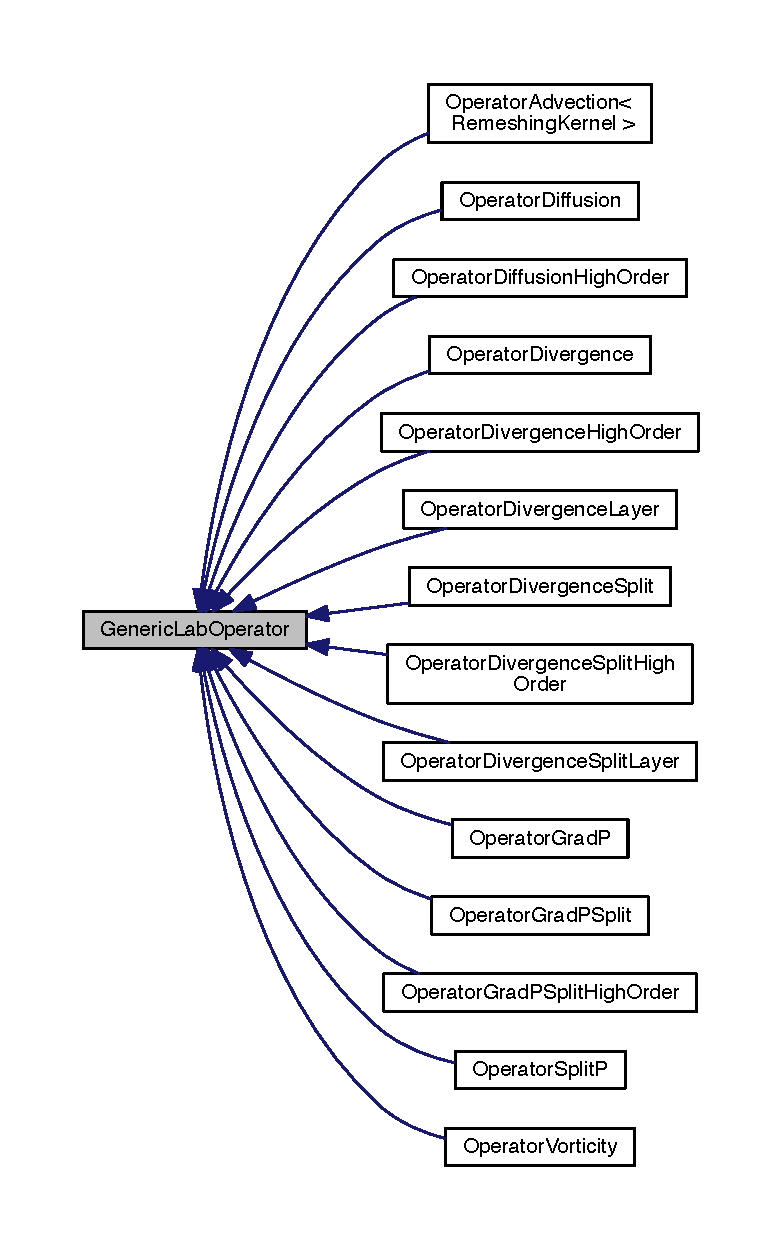
\includegraphics[height=550pt]{df/d01/class_generic_lab_operator__inherit__graph}
\end{center}
\end{figure}
\subsection*{Public Attributes}
\begin{DoxyCompactItemize}
\item 
int \hyperlink{class_generic_lab_operator_a007ab6ad6deb024d839d1d03241672c0}{stencil\+\_\+start} \mbox{[}3\mbox{]}
\item 
int \hyperlink{class_generic_lab_operator_a4daf37ba8c5a018f2b779d8636aba63f}{stencil\+\_\+end} \mbox{[}3\mbox{]}
\end{DoxyCompactItemize}


\subsection{Member Data Documentation}
\hypertarget{class_generic_lab_operator_a4daf37ba8c5a018f2b779d8636aba63f}{}\index{Generic\+Lab\+Operator@{Generic\+Lab\+Operator}!stencil\+\_\+end@{stencil\+\_\+end}}
\index{stencil\+\_\+end@{stencil\+\_\+end}!Generic\+Lab\+Operator@{Generic\+Lab\+Operator}}
\subsubsection[{stencil\+\_\+end}]{\setlength{\rightskip}{0pt plus 5cm}int Generic\+Lab\+Operator\+::stencil\+\_\+end\mbox{[}3\mbox{]}}\label{class_generic_lab_operator_a4daf37ba8c5a018f2b779d8636aba63f}
\hypertarget{class_generic_lab_operator_a007ab6ad6deb024d839d1d03241672c0}{}\index{Generic\+Lab\+Operator@{Generic\+Lab\+Operator}!stencil\+\_\+start@{stencil\+\_\+start}}
\index{stencil\+\_\+start@{stencil\+\_\+start}!Generic\+Lab\+Operator@{Generic\+Lab\+Operator}}
\subsubsection[{stencil\+\_\+start}]{\setlength{\rightskip}{0pt plus 5cm}int Generic\+Lab\+Operator\+::stencil\+\_\+start\mbox{[}3\mbox{]}}\label{class_generic_lab_operator_a007ab6ad6deb024d839d1d03241672c0}


The documentation for this class was generated from the following file\+:\begin{DoxyCompactItemize}
\item 
/\+Users/cconti/\+Desktop/\+Mounts/\+Brutus\+Home/\+Cubism\+U\+P\+\_\+2\+D/source/\hyperlink{_generic_operator_8h}{Generic\+Operator.\+h}\end{DoxyCompactItemize}

\hypertarget{class_generic_operator}{}\section{Generic\+Operator Class Reference}
\label{class_generic_operator}\index{Generic\+Operator@{Generic\+Operator}}


{\ttfamily \#include $<$Generic\+Operator.\+h$>$}



Inheritance diagram for Generic\+Operator\+:\nopagebreak
\begin{figure}[H]
\begin{center}
\leavevmode
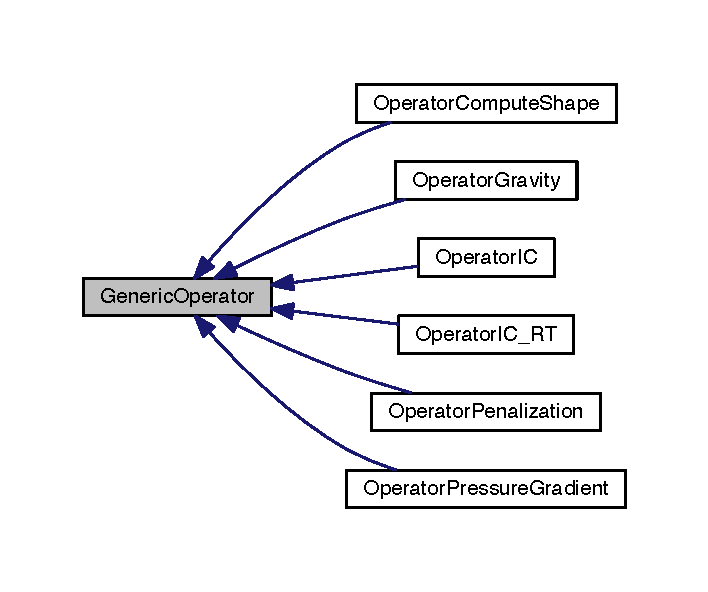
\includegraphics[width=340pt]{dd/db4/class_generic_operator__inherit__graph}
\end{center}
\end{figure}
\subsection*{Public Member Functions}
\begin{DoxyCompactItemize}
\item 
virtual void \hyperlink{class_generic_operator_aacd69e70a1e2d75b97358fca48689a67}{operator()} (const \hyperlink{struct_block_info}{Block\+Info} \&info, \hyperlink{struct_fluid_block}{Fluid\+Block} \&block) const =0
\end{DoxyCompactItemize}


\subsection{Member Function Documentation}
\hypertarget{class_generic_operator_aacd69e70a1e2d75b97358fca48689a67}{}\index{Generic\+Operator@{Generic\+Operator}!operator()@{operator()}}
\index{operator()@{operator()}!Generic\+Operator@{Generic\+Operator}}
\subsubsection[{operator()}]{\setlength{\rightskip}{0pt plus 5cm}virtual void Generic\+Operator\+::operator() (
\begin{DoxyParamCaption}
\item[{const {\bf Block\+Info} \&}]{info, }
\item[{{\bf Fluid\+Block} \&}]{block}
\end{DoxyParamCaption}
) const\hspace{0.3cm}{\ttfamily [pure virtual]}}\label{class_generic_operator_aacd69e70a1e2d75b97358fca48689a67}


Implemented in \hyperlink{class_operator_i_c___r_t_a76857e9f8973fcbfcc8b26e95f55f776}{Operator\+I\+C\+\_\+\+R\+T}, \hyperlink{class_operator_penalization_a55a7fe1ef7cfa3c48c98b0145cd24f00}{Operator\+Penalization}, \hyperlink{class_operator_i_c_adf547defe5168b4bb0181df741a71144}{Operator\+I\+C}, \hyperlink{class_operator_gravity_a7829a016bf4b27c2213493e363515c90}{Operator\+Gravity}, \hyperlink{class_operator_pressure_gradient_a903a0ab2e95bd8d194b147c26086afe8}{Operator\+Pressure\+Gradient}, and \hyperlink{class_operator_compute_shape_ad9d3edd854162a93b5c7212bd694e73a}{Operator\+Compute\+Shape}.



The documentation for this class was generated from the following file\+:\begin{DoxyCompactItemize}
\item 
/\+Users/cconti/\+Desktop/\+Mounts/\+Brutus\+Home/\+Cubism\+U\+P\+\_\+2\+D/source/\hyperlink{_generic_operator_8h}{Generic\+Operator.\+h}\end{DoxyCompactItemize}

\hypertarget{class_grid}{}\section{Grid$<$ Block, allocator $>$ Class Template Reference}
\label{class_grid}\index{Grid$<$ Block, allocator $>$@{Grid$<$ Block, allocator $>$}}


{\ttfamily \#include $<$Grid.\+h$>$}

\subsection*{Public Types}
\begin{DoxyCompactItemize}
\item 
typedef Block \hyperlink{class_grid_a455d62a62799b947e799a28315700b9e}{Block\+Type}
\end{DoxyCompactItemize}
\subsection*{Public Member Functions}
\begin{DoxyCompactItemize}
\item 
\hyperlink{class_grid_a31f48dede8dce2a6fb4260e42c991ec9}{Grid} (const unsigned int \hyperlink{class_grid_a5253120e941ec878f57dd17d5f54cadd}{N\+X}, const unsigned int \hyperlink{class_grid_a8956891d20426acabca4252ec7e299bc}{N\+Y}=1, const unsigned int \hyperlink{class_grid_ad6632ff47c714e008ba88a89b4c1684b}{N\+Z}=1)
\item 
virtual \hyperlink{class_grid_a64f8123459bcfe7c6f2aac0e21a93458}{$\sim$\+Grid} ()
\item 
void \hyperlink{class_grid_a754c47a84c734075e6ccffacb0b4509d}{setup} (const unsigned int n\+X, const unsigned int n\+Y, const unsigned int n\+Z)
\item 
virtual int \hyperlink{class_grid_a68154c3137ad02f44a24d2d75d807fe6}{get\+Blocks\+Per\+Dimension} (int idim) const 
\item 
virtual bool \hyperlink{class_grid_ae2014bfbb3953437effb08202e7cd482}{avail} (unsigned int ix, unsigned int iy=0, unsigned int iz=0) const 
\item 
virtual Block \& \hyperlink{class_grid_a04a6717ea6f8eb51607eaeaba2127055}{operator()} (unsigned int ix, unsigned int iy=0, unsigned int iz=0) const 
\item 
virtual std\+::vector$<$ \hyperlink{struct_block_info}{Block\+Info} $>$ \hyperlink{class_grid_a39aa8cb7fad1abcfe40fdd77d9b72d8a}{get\+Blocks\+Info} () const 
\end{DoxyCompactItemize}
\subsection*{Protected Member Functions}
\begin{DoxyCompactItemize}
\item 
void \hyperlink{class_grid_a3b8f802b38cc4ce4bbd5d2ea9e13f5a3}{\+\_\+dealloc} ()
\item 
void \hyperlink{class_grid_a0d207eb76e069627ebe75c464da7b07a}{\+\_\+alloc} ()
\item 
Block $\ast$ \hyperlink{class_grid_a40a45d5ba147af8742dbe542d36064c4}{\+\_\+linaccess} (const unsigned int idx) const 
\item 
unsigned int \hyperlink{class_grid_aefd1612f9fe87762a3200a10258fe77b}{\+\_\+encode} (const unsigned int ix, const unsigned int iy, const unsigned int iz) const 
\end{DoxyCompactItemize}
\subsection*{Protected Attributes}
\begin{DoxyCompactItemize}
\item 
const unsigned int \hyperlink{class_grid_a9ec3e376ce1de3c9e056a7ccebb34d42}{N}
\item 
const unsigned int \hyperlink{class_grid_a5253120e941ec878f57dd17d5f54cadd}{N\+X}
\item 
const unsigned int \hyperlink{class_grid_a8956891d20426acabca4252ec7e299bc}{N\+Y}
\item 
const unsigned int \hyperlink{class_grid_ad6632ff47c714e008ba88a89b4c1684b}{N\+Z}
\end{DoxyCompactItemize}


\subsection{Member Typedef Documentation}
\hypertarget{class_grid_a455d62a62799b947e799a28315700b9e}{}\index{Grid@{Grid}!Block\+Type@{Block\+Type}}
\index{Block\+Type@{Block\+Type}!Grid@{Grid}}
\subsubsection[{Block\+Type}]{\setlength{\rightskip}{0pt plus 5cm}template$<$typename Block, template$<$ typename X $>$ class allocator = std\+::allocator$>$ typedef Block {\bf Grid}$<$ Block, allocator $>$\+::{\bf Block\+Type}}\label{class_grid_a455d62a62799b947e799a28315700b9e}


\subsection{Constructor \& Destructor Documentation}
\hypertarget{class_grid_a31f48dede8dce2a6fb4260e42c991ec9}{}\index{Grid@{Grid}!Grid@{Grid}}
\index{Grid@{Grid}!Grid@{Grid}}
\subsubsection[{Grid}]{\setlength{\rightskip}{0pt plus 5cm}template$<$typename Block, template$<$ typename X $>$ class allocator = std\+::allocator$>$ {\bf Grid}$<$ Block, allocator $>$\+::{\bf Grid} (
\begin{DoxyParamCaption}
\item[{const unsigned int}]{N\+X, }
\item[{const unsigned int}]{N\+Y = {\ttfamily 1}, }
\item[{const unsigned int}]{N\+Z = {\ttfamily 1}}
\end{DoxyParamCaption}
)\hspace{0.3cm}{\ttfamily [inline]}}\label{class_grid_a31f48dede8dce2a6fb4260e42c991ec9}
\hypertarget{class_grid_a64f8123459bcfe7c6f2aac0e21a93458}{}\index{Grid@{Grid}!````~Grid@{$\sim$\+Grid}}
\index{````~Grid@{$\sim$\+Grid}!Grid@{Grid}}
\subsubsection[{$\sim$\+Grid}]{\setlength{\rightskip}{0pt plus 5cm}template$<$typename Block, template$<$ typename X $>$ class allocator = std\+::allocator$>$ virtual {\bf Grid}$<$ Block, allocator $>$\+::$\sim${\bf Grid} (
\begin{DoxyParamCaption}
{}
\end{DoxyParamCaption}
)\hspace{0.3cm}{\ttfamily [inline]}, {\ttfamily [virtual]}}\label{class_grid_a64f8123459bcfe7c6f2aac0e21a93458}


\subsection{Member Function Documentation}
\hypertarget{class_grid_a0d207eb76e069627ebe75c464da7b07a}{}\index{Grid@{Grid}!\+\_\+alloc@{\+\_\+alloc}}
\index{\+\_\+alloc@{\+\_\+alloc}!Grid@{Grid}}
\subsubsection[{\+\_\+alloc}]{\setlength{\rightskip}{0pt plus 5cm}template$<$typename Block, template$<$ typename X $>$ class allocator = std\+::allocator$>$ void {\bf Grid}$<$ Block, allocator $>$\+::\+\_\+alloc (
\begin{DoxyParamCaption}
{}
\end{DoxyParamCaption}
)\hspace{0.3cm}{\ttfamily [inline]}, {\ttfamily [protected]}}\label{class_grid_a0d207eb76e069627ebe75c464da7b07a}


Here is the caller graph for this function\+:\nopagebreak
\begin{figure}[H]
\begin{center}
\leavevmode
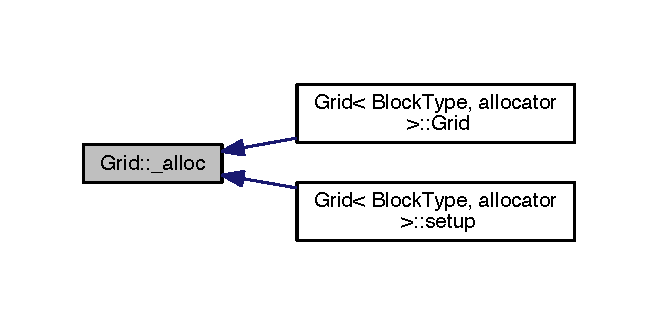
\includegraphics[width=316pt]{da/d74/class_grid_a0d207eb76e069627ebe75c464da7b07a_icgraph}
\end{center}
\end{figure}


\hypertarget{class_grid_a3b8f802b38cc4ce4bbd5d2ea9e13f5a3}{}\index{Grid@{Grid}!\+\_\+dealloc@{\+\_\+dealloc}}
\index{\+\_\+dealloc@{\+\_\+dealloc}!Grid@{Grid}}
\subsubsection[{\+\_\+dealloc}]{\setlength{\rightskip}{0pt plus 5cm}template$<$typename Block, template$<$ typename X $>$ class allocator = std\+::allocator$>$ void {\bf Grid}$<$ Block, allocator $>$\+::\+\_\+dealloc (
\begin{DoxyParamCaption}
{}
\end{DoxyParamCaption}
)\hspace{0.3cm}{\ttfamily [inline]}, {\ttfamily [protected]}}\label{class_grid_a3b8f802b38cc4ce4bbd5d2ea9e13f5a3}


Here is the caller graph for this function\+:\nopagebreak
\begin{figure}[H]
\begin{center}
\leavevmode
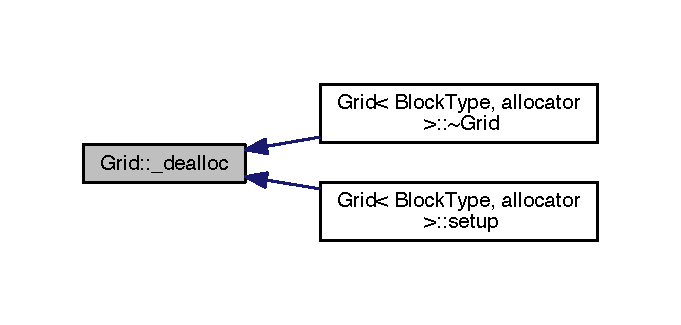
\includegraphics[width=327pt]{da/d74/class_grid_a3b8f802b38cc4ce4bbd5d2ea9e13f5a3_icgraph}
\end{center}
\end{figure}


\hypertarget{class_grid_aefd1612f9fe87762a3200a10258fe77b}{}\index{Grid@{Grid}!\+\_\+encode@{\+\_\+encode}}
\index{\+\_\+encode@{\+\_\+encode}!Grid@{Grid}}
\subsubsection[{\+\_\+encode}]{\setlength{\rightskip}{0pt plus 5cm}template$<$typename Block, template$<$ typename X $>$ class allocator = std\+::allocator$>$ unsigned int {\bf Grid}$<$ Block, allocator $>$\+::\+\_\+encode (
\begin{DoxyParamCaption}
\item[{const unsigned int}]{ix, }
\item[{const unsigned int}]{iy, }
\item[{const unsigned int}]{iz}
\end{DoxyParamCaption}
) const\hspace{0.3cm}{\ttfamily [inline]}, {\ttfamily [protected]}}\label{class_grid_aefd1612f9fe87762a3200a10258fe77b}


Here is the caller graph for this function\+:\nopagebreak
\begin{figure}[H]
\begin{center}
\leavevmode
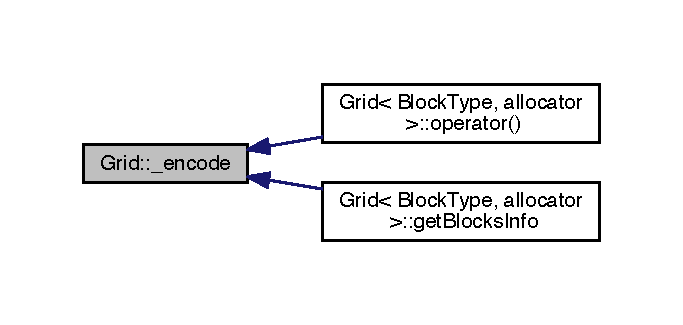
\includegraphics[width=328pt]{da/d74/class_grid_aefd1612f9fe87762a3200a10258fe77b_icgraph}
\end{center}
\end{figure}


\hypertarget{class_grid_a40a45d5ba147af8742dbe542d36064c4}{}\index{Grid@{Grid}!\+\_\+linaccess@{\+\_\+linaccess}}
\index{\+\_\+linaccess@{\+\_\+linaccess}!Grid@{Grid}}
\subsubsection[{\+\_\+linaccess}]{\setlength{\rightskip}{0pt plus 5cm}template$<$typename Block, template$<$ typename X $>$ class allocator = std\+::allocator$>$ Block$\ast$ {\bf Grid}$<$ Block, allocator $>$\+::\+\_\+linaccess (
\begin{DoxyParamCaption}
\item[{const unsigned int}]{idx}
\end{DoxyParamCaption}
) const\hspace{0.3cm}{\ttfamily [inline]}, {\ttfamily [protected]}}\label{class_grid_a40a45d5ba147af8742dbe542d36064c4}


Here is the caller graph for this function\+:\nopagebreak
\begin{figure}[H]
\begin{center}
\leavevmode
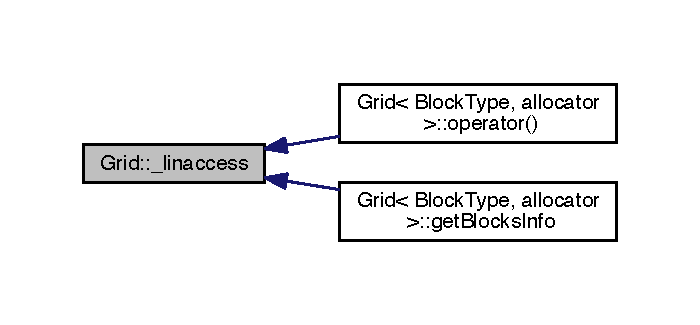
\includegraphics[width=336pt]{da/d74/class_grid_a40a45d5ba147af8742dbe542d36064c4_icgraph}
\end{center}
\end{figure}


\hypertarget{class_grid_ae2014bfbb3953437effb08202e7cd482}{}\index{Grid@{Grid}!avail@{avail}}
\index{avail@{avail}!Grid@{Grid}}
\subsubsection[{avail}]{\setlength{\rightskip}{0pt plus 5cm}template$<$typename Block, template$<$ typename X $>$ class allocator = std\+::allocator$>$ virtual bool {\bf Grid}$<$ Block, allocator $>$\+::avail (
\begin{DoxyParamCaption}
\item[{unsigned int}]{ix, }
\item[{unsigned int}]{iy = {\ttfamily 0}, }
\item[{unsigned int}]{iz = {\ttfamily 0}}
\end{DoxyParamCaption}
) const\hspace{0.3cm}{\ttfamily [inline]}, {\ttfamily [virtual]}}\label{class_grid_ae2014bfbb3953437effb08202e7cd482}


Here is the caller graph for this function\+:\nopagebreak
\begin{figure}[H]
\begin{center}
\leavevmode
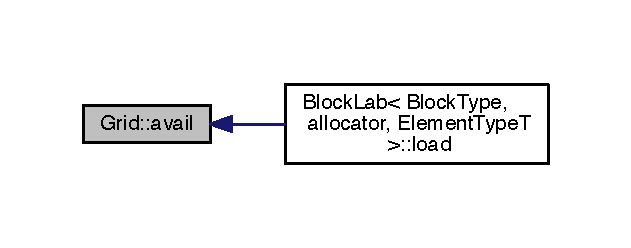
\includegraphics[width=303pt]{da/d74/class_grid_ae2014bfbb3953437effb08202e7cd482_icgraph}
\end{center}
\end{figure}


\hypertarget{class_grid_a39aa8cb7fad1abcfe40fdd77d9b72d8a}{}\index{Grid@{Grid}!get\+Blocks\+Info@{get\+Blocks\+Info}}
\index{get\+Blocks\+Info@{get\+Blocks\+Info}!Grid@{Grid}}
\subsubsection[{get\+Blocks\+Info}]{\setlength{\rightskip}{0pt plus 5cm}template$<$typename Block, template$<$ typename X $>$ class allocator = std\+::allocator$>$ virtual std\+::vector$<${\bf Block\+Info}$>$ {\bf Grid}$<$ Block, allocator $>$\+::get\+Blocks\+Info (
\begin{DoxyParamCaption}
{}
\end{DoxyParamCaption}
) const\hspace{0.3cm}{\ttfamily [inline]}, {\ttfamily [virtual]}}\label{class_grid_a39aa8cb7fad1abcfe40fdd77d9b72d8a}


Here is the caller graph for this function\+:
\nopagebreak
\begin{figure}[H]
\begin{center}
\leavevmode
\includegraphics[height=550pt]{da/d74/class_grid_a39aa8cb7fad1abcfe40fdd77d9b72d8a_icgraph}
\end{center}
\end{figure}


\hypertarget{class_grid_a68154c3137ad02f44a24d2d75d807fe6}{}\index{Grid@{Grid}!get\+Blocks\+Per\+Dimension@{get\+Blocks\+Per\+Dimension}}
\index{get\+Blocks\+Per\+Dimension@{get\+Blocks\+Per\+Dimension}!Grid@{Grid}}
\subsubsection[{get\+Blocks\+Per\+Dimension}]{\setlength{\rightskip}{0pt plus 5cm}template$<$typename Block, template$<$ typename X $>$ class allocator = std\+::allocator$>$ virtual int {\bf Grid}$<$ Block, allocator $>$\+::get\+Blocks\+Per\+Dimension (
\begin{DoxyParamCaption}
\item[{int}]{idim}
\end{DoxyParamCaption}
) const\hspace{0.3cm}{\ttfamily [inline]}, {\ttfamily [virtual]}}\label{class_grid_a68154c3137ad02f44a24d2d75d807fe6}


Here is the caller graph for this function\+:
\nopagebreak
\begin{figure}[H]
\begin{center}
\leavevmode
\includegraphics[width=350pt]{da/d74/class_grid_a68154c3137ad02f44a24d2d75d807fe6_icgraph}
\end{center}
\end{figure}


\hypertarget{class_grid_a04a6717ea6f8eb51607eaeaba2127055}{}\index{Grid@{Grid}!operator()@{operator()}}
\index{operator()@{operator()}!Grid@{Grid}}
\subsubsection[{operator()}]{\setlength{\rightskip}{0pt plus 5cm}template$<$typename Block, template$<$ typename X $>$ class allocator = std\+::allocator$>$ virtual Block\& {\bf Grid}$<$ Block, allocator $>$\+::operator() (
\begin{DoxyParamCaption}
\item[{unsigned int}]{ix, }
\item[{unsigned int}]{iy = {\ttfamily 0}, }
\item[{unsigned int}]{iz = {\ttfamily 0}}
\end{DoxyParamCaption}
) const\hspace{0.3cm}{\ttfamily [inline]}, {\ttfamily [virtual]}}\label{class_grid_a04a6717ea6f8eb51607eaeaba2127055}
\hypertarget{class_grid_a754c47a84c734075e6ccffacb0b4509d}{}\index{Grid@{Grid}!setup@{setup}}
\index{setup@{setup}!Grid@{Grid}}
\subsubsection[{setup}]{\setlength{\rightskip}{0pt plus 5cm}template$<$typename Block, template$<$ typename X $>$ class allocator = std\+::allocator$>$ void {\bf Grid}$<$ Block, allocator $>$\+::setup (
\begin{DoxyParamCaption}
\item[{const unsigned int}]{n\+X, }
\item[{const unsigned int}]{n\+Y, }
\item[{const unsigned int}]{n\+Z}
\end{DoxyParamCaption}
)\hspace{0.3cm}{\ttfamily [inline]}}\label{class_grid_a754c47a84c734075e6ccffacb0b4509d}


Here is the caller graph for this function\+:\nopagebreak
\begin{figure}[H]
\begin{center}
\leavevmode
\includegraphics[width=246pt]{da/d74/class_grid_a754c47a84c734075e6ccffacb0b4509d_icgraph}
\end{center}
\end{figure}




\subsection{Member Data Documentation}
\hypertarget{class_grid_a9ec3e376ce1de3c9e056a7ccebb34d42}{}\index{Grid@{Grid}!N@{N}}
\index{N@{N}!Grid@{Grid}}
\subsubsection[{N}]{\setlength{\rightskip}{0pt plus 5cm}template$<$typename Block, template$<$ typename X $>$ class allocator = std\+::allocator$>$ const unsigned int {\bf Grid}$<$ Block, allocator $>$\+::N\hspace{0.3cm}{\ttfamily [protected]}}\label{class_grid_a9ec3e376ce1de3c9e056a7ccebb34d42}
\hypertarget{class_grid_a5253120e941ec878f57dd17d5f54cadd}{}\index{Grid@{Grid}!N\+X@{N\+X}}
\index{N\+X@{N\+X}!Grid@{Grid}}
\subsubsection[{N\+X}]{\setlength{\rightskip}{0pt plus 5cm}template$<$typename Block, template$<$ typename X $>$ class allocator = std\+::allocator$>$ const unsigned int {\bf Grid}$<$ Block, allocator $>$\+::N\+X\hspace{0.3cm}{\ttfamily [protected]}}\label{class_grid_a5253120e941ec878f57dd17d5f54cadd}
\hypertarget{class_grid_a8956891d20426acabca4252ec7e299bc}{}\index{Grid@{Grid}!N\+Y@{N\+Y}}
\index{N\+Y@{N\+Y}!Grid@{Grid}}
\subsubsection[{N\+Y}]{\setlength{\rightskip}{0pt plus 5cm}template$<$typename Block, template$<$ typename X $>$ class allocator = std\+::allocator$>$ const unsigned int {\bf Grid}$<$ Block, allocator $>$\+::N\+Y\hspace{0.3cm}{\ttfamily [protected]}}\label{class_grid_a8956891d20426acabca4252ec7e299bc}
\hypertarget{class_grid_ad6632ff47c714e008ba88a89b4c1684b}{}\index{Grid@{Grid}!N\+Z@{N\+Z}}
\index{N\+Z@{N\+Z}!Grid@{Grid}}
\subsubsection[{N\+Z}]{\setlength{\rightskip}{0pt plus 5cm}template$<$typename Block, template$<$ typename X $>$ class allocator = std\+::allocator$>$ const unsigned int {\bf Grid}$<$ Block, allocator $>$\+::N\+Z\hspace{0.3cm}{\ttfamily [protected]}}\label{class_grid_ad6632ff47c714e008ba88a89b4c1684b}


The documentation for this class was generated from the following file\+:\begin{DoxyCompactItemize}
\item 
/\+Users/cconti/\+Desktop/\+Mounts/\+Brutus\+Home/\+Cubism\+U\+P\+\_\+2\+D/\+Cubism/\hyperlink{_grid_8h}{Grid.\+h}\end{DoxyCompactItemize}

\hypertarget{class_grid_morton}{}\section{Grid\+Morton$<$ T\+Grid $>$ Class Template Reference}
\label{class_grid_morton}\index{Grid\+Morton$<$ T\+Grid $>$@{Grid\+Morton$<$ T\+Grid $>$}}


{\ttfamily \#include $<$Grid\+Morton.\+h$>$}



Inheritance diagram for Grid\+Morton$<$ T\+Grid $>$\+:
% FIG 0


Collaboration diagram for Grid\+Morton$<$ T\+Grid $>$\+:
% FIG 1
\subsection*{Public Types}
\begin{DoxyCompactItemize}
\item 
typedef T\+Grid\+::\+Block\+Type \hyperlink{class_grid_morton_a015e2b8a69c60cf84a8f1b5b42ce5b1c}{T\+Block}
\end{DoxyCompactItemize}
\subsection*{Public Member Functions}
\begin{DoxyCompactItemize}
\item 
\hyperlink{class_grid_morton_a811a018e13f854a40dbbbc17ba50e13b}{Grid\+Morton} (unsigned int n\+X, unsigned int n\+Y=1, unsigned int n\+Z=1)
\item 
\hyperlink{class_grid_morton_a015e2b8a69c60cf84a8f1b5b42ce5b1c}{T\+Block} \& \hyperlink{class_grid_morton_a5c224b606ea7e4ad490430f3d3ff2d8c}{operator()} (unsigned int ix, unsigned int iy=0, unsigned int iz=0) const 
\item 
vector$<$ \hyperlink{struct_block_info}{Block\+Info} $>$ \hyperlink{class_grid_morton_a78bda35a781c2ffb48dadcac1e59a901}{get\+Blocks\+Info} () const 
\end{DoxyCompactItemize}


\subsection{Member Typedef Documentation}
\hypertarget{class_grid_morton_a015e2b8a69c60cf84a8f1b5b42ce5b1c}{}\index{Grid\+Morton@{Grid\+Morton}!T\+Block@{T\+Block}}
\index{T\+Block@{T\+Block}!Grid\+Morton@{Grid\+Morton}}
\subsubsection[{T\+Block}]{\setlength{\rightskip}{0pt plus 5cm}template$<$typename T\+Grid $>$ typedef T\+Grid\+::\+Block\+Type {\bf Grid\+Morton}$<$ T\+Grid $>$\+::{\bf T\+Block}}\label{class_grid_morton_a015e2b8a69c60cf84a8f1b5b42ce5b1c}


\subsection{Constructor \& Destructor Documentation}
\hypertarget{class_grid_morton_a811a018e13f854a40dbbbc17ba50e13b}{}\index{Grid\+Morton@{Grid\+Morton}!Grid\+Morton@{Grid\+Morton}}
\index{Grid\+Morton@{Grid\+Morton}!Grid\+Morton@{Grid\+Morton}}
\subsubsection[{Grid\+Morton}]{\setlength{\rightskip}{0pt plus 5cm}template$<$typename T\+Grid $>$ {\bf Grid\+Morton}$<$ T\+Grid $>$\+::{\bf Grid\+Morton} (
\begin{DoxyParamCaption}
\item[{unsigned int}]{n\+X, }
\item[{unsigned int}]{n\+Y = {\ttfamily 1}, }
\item[{unsigned int}]{n\+Z = {\ttfamily 1}}
\end{DoxyParamCaption}
)\hspace{0.3cm}{\ttfamily [inline]}}\label{class_grid_morton_a811a018e13f854a40dbbbc17ba50e13b}


\subsection{Member Function Documentation}
\hypertarget{class_grid_morton_a78bda35a781c2ffb48dadcac1e59a901}{}\index{Grid\+Morton@{Grid\+Morton}!get\+Blocks\+Info@{get\+Blocks\+Info}}
\index{get\+Blocks\+Info@{get\+Blocks\+Info}!Grid\+Morton@{Grid\+Morton}}
\subsubsection[{get\+Blocks\+Info}]{\setlength{\rightskip}{0pt plus 5cm}template$<$typename T\+Grid $>$ vector$<${\bf Block\+Info}$>$ {\bf Grid\+Morton}$<$ T\+Grid $>$\+::get\+Blocks\+Info (
\begin{DoxyParamCaption}
{}
\end{DoxyParamCaption}
) const\hspace{0.3cm}{\ttfamily [inline]}}\label{class_grid_morton_a78bda35a781c2ffb48dadcac1e59a901}
\hypertarget{class_grid_morton_a5c224b606ea7e4ad490430f3d3ff2d8c}{}\index{Grid\+Morton@{Grid\+Morton}!operator()@{operator()}}
\index{operator()@{operator()}!Grid\+Morton@{Grid\+Morton}}
\subsubsection[{operator()}]{\setlength{\rightskip}{0pt plus 5cm}template$<$typename T\+Grid $>$ {\bf T\+Block}\& {\bf Grid\+Morton}$<$ T\+Grid $>$\+::operator() (
\begin{DoxyParamCaption}
\item[{unsigned int}]{ix, }
\item[{unsigned int}]{iy = {\ttfamily 0}, }
\item[{unsigned int}]{iz = {\ttfamily 0}}
\end{DoxyParamCaption}
) const\hspace{0.3cm}{\ttfamily [inline]}}\label{class_grid_morton_a5c224b606ea7e4ad490430f3d3ff2d8c}


Here is the call graph for this function\+:
% FIG 2




The documentation for this class was generated from the following file\+:\begin{DoxyCompactItemize}
\item 
/\+Users/cconti/\+Desktop/\+Mounts/\+Brutus\+Home/\+Seed/\+Cubism\+U\+P\+\_\+2\+D/\+Cubism/\hyperlink{_grid_morton_8h}{Grid\+Morton.\+h}\end{DoxyCompactItemize}

\hypertarget{class_grid_m_p_i}{}\section{Grid\+M\+P\+I$<$ T\+Grid $>$ Class Template Reference}
\label{class_grid_m_p_i}\index{Grid\+M\+P\+I$<$ T\+Grid $>$@{Grid\+M\+P\+I$<$ T\+Grid $>$}}


{\ttfamily \#include $<$Grid\+M\+P\+I.\+h$>$}



Inheritance diagram for Grid\+M\+P\+I$<$ T\+Grid $>$\+:\nopagebreak
\begin{figure}[H]
\begin{center}
\leavevmode
\includegraphics[width=175pt]{de/dce/class_grid_m_p_i__inherit__graph}
\end{center}
\end{figure}


Collaboration diagram for Grid\+M\+P\+I$<$ T\+Grid $>$\+:\nopagebreak
\begin{figure}[H]
\begin{center}
\leavevmode
\includegraphics[width=175pt]{dc/ddd/class_grid_m_p_i__coll__graph}
\end{center}
\end{figure}
\subsection*{Public Member Functions}
\begin{DoxyCompactItemize}
\item 
\hyperlink{class_grid_m_p_i_ad515efd9d7bd9560eed5e958950cbb4d}{Grid\+M\+P\+I} (const int npe\+X, const int npe\+Y, const int npe\+Z, const int n\+X, const int n\+Y=1, const int n\+Z=1, const bool b\+Periodic\+X=true, const bool b\+Periodic\+Y=true, const bool b\+Periodic\+Z=true)
\item 
\hyperlink{class_grid_m_p_i_a22874a9873aacbc4813f8f47606c89b6}{$\sim$\+Grid\+M\+P\+I} ()
\item 
vector$<$ \hyperlink{struct_block_info}{Block\+Info} $>$ \hyperlink{class_grid_m_p_i_abd9d87482f590729369816a9191fec90}{get\+Blocks\+Info} () const 
\item 
vector$<$ \hyperlink{struct_block_info}{Block\+Info} $>$ \hyperlink{class_grid_m_p_i_ae68d98fcfc60a139a468b2b66743a815}{get\+Resident\+Blocks\+Info} () const 
\item 
virtual bool \hyperlink{class_grid_m_p_i_a09fb63dc01bf37404fbce026dc52f8da}{avail} (int ix, int iy=0, int iz=0) const 
\item 
Block \& \hyperlink{class_grid_m_p_i_ae21841fb3c6ff3127647610a62388b6d}{operator()} (int ix, int iy=0, int iz=0) const 
\item 
{\footnotesize template$<$typename Processing $>$ }\\\hyperlink{class_synchronizer_m_p_i}{Synchronizer\+M\+P\+I} \& \hyperlink{class_grid_m_p_i_adbd8d6fb9ec2dd16e9a8317fa573d000}{sync} (Processing \&p)
\item 
{\footnotesize template$<$typename Processing $>$ }\\const \hyperlink{class_synchronizer_m_p_i}{Synchronizer\+M\+P\+I} \& \hyperlink{class_grid_m_p_i_ae57bf08859c39ed4ea3ee3031b289352}{get\+\_\+\+Synchronizer\+M\+P\+I} (Processing \&p) const 
\item 
int \hyperlink{class_grid_m_p_i_a2d743c8605ca373df9f174b350c06d76}{get\+Resident\+Blocks\+Per\+Dimension} (int idim) const 
\item 
int \hyperlink{class_grid_m_p_i_aad5685d311020dd70b9af3b08f51450f}{get\+Blocks\+Per\+Dimension} (int idim) const 
\item 
void \hyperlink{class_grid_m_p_i_afc77b34860081db4e179c6bd5ec4a04c}{peindex} (int \hyperlink{class_grid_m_p_i_a18aa2c80d121cc50339949d8c3d0d547}{mypeindex}\mbox{[}3\mbox{]}) const 
\item 
size\+\_\+t \hyperlink{class_grid_m_p_i_a225c750fb4e70ed908fb8ec485b31762}{get\+Time\+Stamp} () const 
\item 
M\+P\+I\+::\+Cartcomm \hyperlink{class_grid_m_p_i_a0368859fa3e4d49b1a6a52daa5789712}{get\+Cart\+Comm} () const 
\end{DoxyCompactItemize}
\subsection*{Protected Attributes}
\begin{DoxyCompactItemize}
\item 
map$<$ \hyperlink{struct_stencil_info}{Stencil\+Info}, \hyperlink{class_synchronizer_m_p_i}{Synchronizer\+M\+P\+I} $\ast$ $>$ \hyperlink{class_grid_m_p_i_a2630fe6ea5a92bc46e122bce621143e5}{Synchronizer\+M\+P\+Is}
\item 
M\+P\+I\+::\+Cartcomm \hyperlink{class_grid_m_p_i_a11225861787838aeb43f9a6be7a5736b}{cartcomm}
\item 
int \hyperlink{class_grid_m_p_i_ac06426dbf8b56ab9f642f38b99a8ff58}{myrank}
\item 
int \hyperlink{class_grid_m_p_i_a18aa2c80d121cc50339949d8c3d0d547}{mypeindex} \mbox{[}3\mbox{]}
\item 
int \hyperlink{class_grid_m_p_i_ad23be40f0e498f46f215c36e0a00546c}{pesize} \mbox{[}3\mbox{]}
\item 
bool \hyperlink{class_grid_m_p_i_a5376cf349ce2d317bddc363907b22f69}{periodic} \mbox{[}3\mbox{]}
\item 
int \hyperlink{class_grid_m_p_i_a18238a13a4e9d9448ff9562560d5eadf}{mybpd} \mbox{[}3\mbox{]}
\item 
int \hyperlink{class_grid_m_p_i_a33aea82975cdfa2b3f017ee35fab6c5b}{myblockstotalsize}
\item 
int \hyperlink{class_grid_m_p_i_a9c0c291e8619844c31afa37d884e7805}{blocksize} \mbox{[}3\mbox{]}
\item 
vector$<$ \hyperlink{struct_block_info}{Block\+Info} $>$ \hyperlink{class_grid_m_p_i_ad5256ab6f6cef049008518d5d2ab7bdb}{cached\+\_\+blockinfo}
\end{DoxyCompactItemize}
\subsection*{Friends}
\begin{DoxyCompactItemize}
\item 
class \hyperlink{class_grid_m_p_i_a4d6cf8eb005be8cd74ca25544993aca2}{Synchronizer\+M\+P\+I}
\end{DoxyCompactItemize}


\subsection{Constructor \& Destructor Documentation}
\hypertarget{class_grid_m_p_i_ad515efd9d7bd9560eed5e958950cbb4d}{}\index{Grid\+M\+P\+I@{Grid\+M\+P\+I}!Grid\+M\+P\+I@{Grid\+M\+P\+I}}
\index{Grid\+M\+P\+I@{Grid\+M\+P\+I}!Grid\+M\+P\+I@{Grid\+M\+P\+I}}
\subsubsection[{Grid\+M\+P\+I}]{\setlength{\rightskip}{0pt plus 5cm}template$<$typename T\+Grid$>$ {\bf Grid\+M\+P\+I}$<$ T\+Grid $>$\+::{\bf Grid\+M\+P\+I} (
\begin{DoxyParamCaption}
\item[{const int}]{npe\+X, }
\item[{const int}]{npe\+Y, }
\item[{const int}]{npe\+Z, }
\item[{const int}]{n\+X, }
\item[{const int}]{n\+Y = {\ttfamily 1}, }
\item[{const int}]{n\+Z = {\ttfamily 1}, }
\item[{const bool}]{b\+Periodic\+X = {\ttfamily true}, }
\item[{const bool}]{b\+Periodic\+Y = {\ttfamily true}, }
\item[{const bool}]{b\+Periodic\+Z = {\ttfamily true}}
\end{DoxyParamCaption}
)\hspace{0.3cm}{\ttfamily [inline]}}\label{class_grid_m_p_i_ad515efd9d7bd9560eed5e958950cbb4d}
\hypertarget{class_grid_m_p_i_a22874a9873aacbc4813f8f47606c89b6}{}\index{Grid\+M\+P\+I@{Grid\+M\+P\+I}!````~Grid\+M\+P\+I@{$\sim$\+Grid\+M\+P\+I}}
\index{````~Grid\+M\+P\+I@{$\sim$\+Grid\+M\+P\+I}!Grid\+M\+P\+I@{Grid\+M\+P\+I}}
\subsubsection[{$\sim$\+Grid\+M\+P\+I}]{\setlength{\rightskip}{0pt plus 5cm}template$<$typename T\+Grid$>$ {\bf Grid\+M\+P\+I}$<$ T\+Grid $>$\+::$\sim${\bf Grid\+M\+P\+I} (
\begin{DoxyParamCaption}
{}
\end{DoxyParamCaption}
)\hspace{0.3cm}{\ttfamily [inline]}}\label{class_grid_m_p_i_a22874a9873aacbc4813f8f47606c89b6}


\subsection{Member Function Documentation}
\hypertarget{class_grid_m_p_i_a09fb63dc01bf37404fbce026dc52f8da}{}\index{Grid\+M\+P\+I@{Grid\+M\+P\+I}!avail@{avail}}
\index{avail@{avail}!Grid\+M\+P\+I@{Grid\+M\+P\+I}}
\subsubsection[{avail}]{\setlength{\rightskip}{0pt plus 5cm}template$<$typename T\+Grid$>$ virtual bool {\bf Grid\+M\+P\+I}$<$ T\+Grid $>$\+::avail (
\begin{DoxyParamCaption}
\item[{int}]{ix, }
\item[{int}]{iy = {\ttfamily 0}, }
\item[{int}]{iz = {\ttfamily 0}}
\end{DoxyParamCaption}
) const\hspace{0.3cm}{\ttfamily [inline]}, {\ttfamily [virtual]}}\label{class_grid_m_p_i_a09fb63dc01bf37404fbce026dc52f8da}
\hypertarget{class_grid_m_p_i_ae57bf08859c39ed4ea3ee3031b289352}{}\index{Grid\+M\+P\+I@{Grid\+M\+P\+I}!get\+\_\+\+Synchronizer\+M\+P\+I@{get\+\_\+\+Synchronizer\+M\+P\+I}}
\index{get\+\_\+\+Synchronizer\+M\+P\+I@{get\+\_\+\+Synchronizer\+M\+P\+I}!Grid\+M\+P\+I@{Grid\+M\+P\+I}}
\subsubsection[{get\+\_\+\+Synchronizer\+M\+P\+I}]{\setlength{\rightskip}{0pt plus 5cm}template$<$typename T\+Grid$>$ template$<$typename Processing $>$ const {\bf Synchronizer\+M\+P\+I}\& {\bf Grid\+M\+P\+I}$<$ T\+Grid $>$\+::get\+\_\+\+Synchronizer\+M\+P\+I (
\begin{DoxyParamCaption}
\item[{Processing \&}]{p}
\end{DoxyParamCaption}
) const\hspace{0.3cm}{\ttfamily [inline]}}\label{class_grid_m_p_i_ae57bf08859c39ed4ea3ee3031b289352}
\hypertarget{class_grid_m_p_i_abd9d87482f590729369816a9191fec90}{}\index{Grid\+M\+P\+I@{Grid\+M\+P\+I}!get\+Blocks\+Info@{get\+Blocks\+Info}}
\index{get\+Blocks\+Info@{get\+Blocks\+Info}!Grid\+M\+P\+I@{Grid\+M\+P\+I}}
\subsubsection[{get\+Blocks\+Info}]{\setlength{\rightskip}{0pt plus 5cm}template$<$typename T\+Grid$>$ vector$<${\bf Block\+Info}$>$ {\bf Grid\+M\+P\+I}$<$ T\+Grid $>$\+::get\+Blocks\+Info (
\begin{DoxyParamCaption}
{}
\end{DoxyParamCaption}
) const\hspace{0.3cm}{\ttfamily [inline]}}\label{class_grid_m_p_i_abd9d87482f590729369816a9191fec90}
\hypertarget{class_grid_m_p_i_aad5685d311020dd70b9af3b08f51450f}{}\index{Grid\+M\+P\+I@{Grid\+M\+P\+I}!get\+Blocks\+Per\+Dimension@{get\+Blocks\+Per\+Dimension}}
\index{get\+Blocks\+Per\+Dimension@{get\+Blocks\+Per\+Dimension}!Grid\+M\+P\+I@{Grid\+M\+P\+I}}
\subsubsection[{get\+Blocks\+Per\+Dimension}]{\setlength{\rightskip}{0pt plus 5cm}template$<$typename T\+Grid$>$ int {\bf Grid\+M\+P\+I}$<$ T\+Grid $>$\+::get\+Blocks\+Per\+Dimension (
\begin{DoxyParamCaption}
\item[{int}]{idim}
\end{DoxyParamCaption}
) const\hspace{0.3cm}{\ttfamily [inline]}}\label{class_grid_m_p_i_aad5685d311020dd70b9af3b08f51450f}


Here is the caller graph for this function\+:\nopagebreak
\begin{figure}[H]
\begin{center}
\leavevmode
\includegraphics[width=350pt]{d9/d3c/class_grid_m_p_i_aad5685d311020dd70b9af3b08f51450f_icgraph}
\end{center}
\end{figure}


\hypertarget{class_grid_m_p_i_a0368859fa3e4d49b1a6a52daa5789712}{}\index{Grid\+M\+P\+I@{Grid\+M\+P\+I}!get\+Cart\+Comm@{get\+Cart\+Comm}}
\index{get\+Cart\+Comm@{get\+Cart\+Comm}!Grid\+M\+P\+I@{Grid\+M\+P\+I}}
\subsubsection[{get\+Cart\+Comm}]{\setlength{\rightskip}{0pt plus 5cm}template$<$typename T\+Grid$>$ M\+P\+I\+::\+Cartcomm {\bf Grid\+M\+P\+I}$<$ T\+Grid $>$\+::get\+Cart\+Comm (
\begin{DoxyParamCaption}
{}
\end{DoxyParamCaption}
) const\hspace{0.3cm}{\ttfamily [inline]}}\label{class_grid_m_p_i_a0368859fa3e4d49b1a6a52daa5789712}
\hypertarget{class_grid_m_p_i_ae68d98fcfc60a139a468b2b66743a815}{}\index{Grid\+M\+P\+I@{Grid\+M\+P\+I}!get\+Resident\+Blocks\+Info@{get\+Resident\+Blocks\+Info}}
\index{get\+Resident\+Blocks\+Info@{get\+Resident\+Blocks\+Info}!Grid\+M\+P\+I@{Grid\+M\+P\+I}}
\subsubsection[{get\+Resident\+Blocks\+Info}]{\setlength{\rightskip}{0pt plus 5cm}template$<$typename T\+Grid$>$ vector$<${\bf Block\+Info}$>$ {\bf Grid\+M\+P\+I}$<$ T\+Grid $>$\+::get\+Resident\+Blocks\+Info (
\begin{DoxyParamCaption}
{}
\end{DoxyParamCaption}
) const\hspace{0.3cm}{\ttfamily [inline]}}\label{class_grid_m_p_i_ae68d98fcfc60a139a468b2b66743a815}
\hypertarget{class_grid_m_p_i_a2d743c8605ca373df9f174b350c06d76}{}\index{Grid\+M\+P\+I@{Grid\+M\+P\+I}!get\+Resident\+Blocks\+Per\+Dimension@{get\+Resident\+Blocks\+Per\+Dimension}}
\index{get\+Resident\+Blocks\+Per\+Dimension@{get\+Resident\+Blocks\+Per\+Dimension}!Grid\+M\+P\+I@{Grid\+M\+P\+I}}
\subsubsection[{get\+Resident\+Blocks\+Per\+Dimension}]{\setlength{\rightskip}{0pt plus 5cm}template$<$typename T\+Grid$>$ int {\bf Grid\+M\+P\+I}$<$ T\+Grid $>$\+::get\+Resident\+Blocks\+Per\+Dimension (
\begin{DoxyParamCaption}
\item[{int}]{idim}
\end{DoxyParamCaption}
) const\hspace{0.3cm}{\ttfamily [inline]}}\label{class_grid_m_p_i_a2d743c8605ca373df9f174b350c06d76}
\hypertarget{class_grid_m_p_i_a225c750fb4e70ed908fb8ec485b31762}{}\index{Grid\+M\+P\+I@{Grid\+M\+P\+I}!get\+Time\+Stamp@{get\+Time\+Stamp}}
\index{get\+Time\+Stamp@{get\+Time\+Stamp}!Grid\+M\+P\+I@{Grid\+M\+P\+I}}
\subsubsection[{get\+Time\+Stamp}]{\setlength{\rightskip}{0pt plus 5cm}template$<$typename T\+Grid$>$ size\+\_\+t {\bf Grid\+M\+P\+I}$<$ T\+Grid $>$\+::get\+Time\+Stamp (
\begin{DoxyParamCaption}
{}
\end{DoxyParamCaption}
) const\hspace{0.3cm}{\ttfamily [inline]}}\label{class_grid_m_p_i_a225c750fb4e70ed908fb8ec485b31762}
\hypertarget{class_grid_m_p_i_ae21841fb3c6ff3127647610a62388b6d}{}\index{Grid\+M\+P\+I@{Grid\+M\+P\+I}!operator()@{operator()}}
\index{operator()@{operator()}!Grid\+M\+P\+I@{Grid\+M\+P\+I}}
\subsubsection[{operator()}]{\setlength{\rightskip}{0pt plus 5cm}template$<$typename T\+Grid$>$ Block\& {\bf Grid\+M\+P\+I}$<$ T\+Grid $>$\+::operator() (
\begin{DoxyParamCaption}
\item[{int}]{ix, }
\item[{int}]{iy = {\ttfamily 0}, }
\item[{int}]{iz = {\ttfamily 0}}
\end{DoxyParamCaption}
) const\hspace{0.3cm}{\ttfamily [inline]}}\label{class_grid_m_p_i_ae21841fb3c6ff3127647610a62388b6d}
\hypertarget{class_grid_m_p_i_afc77b34860081db4e179c6bd5ec4a04c}{}\index{Grid\+M\+P\+I@{Grid\+M\+P\+I}!peindex@{peindex}}
\index{peindex@{peindex}!Grid\+M\+P\+I@{Grid\+M\+P\+I}}
\subsubsection[{peindex}]{\setlength{\rightskip}{0pt plus 5cm}template$<$typename T\+Grid$>$ void {\bf Grid\+M\+P\+I}$<$ T\+Grid $>$\+::peindex (
\begin{DoxyParamCaption}
\item[{int}]{mypeindex\mbox{[}3\mbox{]}}
\end{DoxyParamCaption}
) const\hspace{0.3cm}{\ttfamily [inline]}}\label{class_grid_m_p_i_afc77b34860081db4e179c6bd5ec4a04c}
\hypertarget{class_grid_m_p_i_adbd8d6fb9ec2dd16e9a8317fa573d000}{}\index{Grid\+M\+P\+I@{Grid\+M\+P\+I}!sync@{sync}}
\index{sync@{sync}!Grid\+M\+P\+I@{Grid\+M\+P\+I}}
\subsubsection[{sync}]{\setlength{\rightskip}{0pt plus 5cm}template$<$typename T\+Grid$>$ template$<$typename Processing $>$ {\bf Synchronizer\+M\+P\+I}\& {\bf Grid\+M\+P\+I}$<$ T\+Grid $>$\+::sync (
\begin{DoxyParamCaption}
\item[{Processing \&}]{p}
\end{DoxyParamCaption}
)\hspace{0.3cm}{\ttfamily [inline]}}\label{class_grid_m_p_i_adbd8d6fb9ec2dd16e9a8317fa573d000}


Here is the call graph for this function\+:\nopagebreak
\begin{figure}[H]
\begin{center}
\leavevmode
\includegraphics[width=350pt]{d9/d3c/class_grid_m_p_i_adbd8d6fb9ec2dd16e9a8317fa573d000_cgraph}
\end{center}
\end{figure}




\subsection{Friends And Related Function Documentation}
\hypertarget{class_grid_m_p_i_a4d6cf8eb005be8cd74ca25544993aca2}{}\index{Grid\+M\+P\+I@{Grid\+M\+P\+I}!Synchronizer\+M\+P\+I@{Synchronizer\+M\+P\+I}}
\index{Synchronizer\+M\+P\+I@{Synchronizer\+M\+P\+I}!Grid\+M\+P\+I@{Grid\+M\+P\+I}}
\subsubsection[{Synchronizer\+M\+P\+I}]{\setlength{\rightskip}{0pt plus 5cm}template$<$typename T\+Grid$>$ friend class {\bf Synchronizer\+M\+P\+I}\hspace{0.3cm}{\ttfamily [friend]}}\label{class_grid_m_p_i_a4d6cf8eb005be8cd74ca25544993aca2}


\subsection{Member Data Documentation}
\hypertarget{class_grid_m_p_i_a9c0c291e8619844c31afa37d884e7805}{}\index{Grid\+M\+P\+I@{Grid\+M\+P\+I}!blocksize@{blocksize}}
\index{blocksize@{blocksize}!Grid\+M\+P\+I@{Grid\+M\+P\+I}}
\subsubsection[{blocksize}]{\setlength{\rightskip}{0pt plus 5cm}template$<$typename T\+Grid$>$ int {\bf Grid\+M\+P\+I}$<$ T\+Grid $>$\+::blocksize\mbox{[}3\mbox{]}\hspace{0.3cm}{\ttfamily [protected]}}\label{class_grid_m_p_i_a9c0c291e8619844c31afa37d884e7805}
\hypertarget{class_grid_m_p_i_ad5256ab6f6cef049008518d5d2ab7bdb}{}\index{Grid\+M\+P\+I@{Grid\+M\+P\+I}!cached\+\_\+blockinfo@{cached\+\_\+blockinfo}}
\index{cached\+\_\+blockinfo@{cached\+\_\+blockinfo}!Grid\+M\+P\+I@{Grid\+M\+P\+I}}
\subsubsection[{cached\+\_\+blockinfo}]{\setlength{\rightskip}{0pt plus 5cm}template$<$typename T\+Grid$>$ vector$<${\bf Block\+Info}$>$ {\bf Grid\+M\+P\+I}$<$ T\+Grid $>$\+::cached\+\_\+blockinfo\hspace{0.3cm}{\ttfamily [protected]}}\label{class_grid_m_p_i_ad5256ab6f6cef049008518d5d2ab7bdb}
\hypertarget{class_grid_m_p_i_a11225861787838aeb43f9a6be7a5736b}{}\index{Grid\+M\+P\+I@{Grid\+M\+P\+I}!cartcomm@{cartcomm}}
\index{cartcomm@{cartcomm}!Grid\+M\+P\+I@{Grid\+M\+P\+I}}
\subsubsection[{cartcomm}]{\setlength{\rightskip}{0pt plus 5cm}template$<$typename T\+Grid$>$ M\+P\+I\+::\+Cartcomm {\bf Grid\+M\+P\+I}$<$ T\+Grid $>$\+::cartcomm\hspace{0.3cm}{\ttfamily [protected]}}\label{class_grid_m_p_i_a11225861787838aeb43f9a6be7a5736b}
\hypertarget{class_grid_m_p_i_a33aea82975cdfa2b3f017ee35fab6c5b}{}\index{Grid\+M\+P\+I@{Grid\+M\+P\+I}!myblockstotalsize@{myblockstotalsize}}
\index{myblockstotalsize@{myblockstotalsize}!Grid\+M\+P\+I@{Grid\+M\+P\+I}}
\subsubsection[{myblockstotalsize}]{\setlength{\rightskip}{0pt plus 5cm}template$<$typename T\+Grid$>$ int {\bf Grid\+M\+P\+I}$<$ T\+Grid $>$\+::myblockstotalsize\hspace{0.3cm}{\ttfamily [protected]}}\label{class_grid_m_p_i_a33aea82975cdfa2b3f017ee35fab6c5b}
\hypertarget{class_grid_m_p_i_a18238a13a4e9d9448ff9562560d5eadf}{}\index{Grid\+M\+P\+I@{Grid\+M\+P\+I}!mybpd@{mybpd}}
\index{mybpd@{mybpd}!Grid\+M\+P\+I@{Grid\+M\+P\+I}}
\subsubsection[{mybpd}]{\setlength{\rightskip}{0pt plus 5cm}template$<$typename T\+Grid$>$ int {\bf Grid\+M\+P\+I}$<$ T\+Grid $>$\+::mybpd\mbox{[}3\mbox{]}\hspace{0.3cm}{\ttfamily [protected]}}\label{class_grid_m_p_i_a18238a13a4e9d9448ff9562560d5eadf}
\hypertarget{class_grid_m_p_i_a18aa2c80d121cc50339949d8c3d0d547}{}\index{Grid\+M\+P\+I@{Grid\+M\+P\+I}!mypeindex@{mypeindex}}
\index{mypeindex@{mypeindex}!Grid\+M\+P\+I@{Grid\+M\+P\+I}}
\subsubsection[{mypeindex}]{\setlength{\rightskip}{0pt plus 5cm}template$<$typename T\+Grid$>$ int {\bf Grid\+M\+P\+I}$<$ T\+Grid $>$\+::mypeindex\mbox{[}3\mbox{]}\hspace{0.3cm}{\ttfamily [protected]}}\label{class_grid_m_p_i_a18aa2c80d121cc50339949d8c3d0d547}
\hypertarget{class_grid_m_p_i_ac06426dbf8b56ab9f642f38b99a8ff58}{}\index{Grid\+M\+P\+I@{Grid\+M\+P\+I}!myrank@{myrank}}
\index{myrank@{myrank}!Grid\+M\+P\+I@{Grid\+M\+P\+I}}
\subsubsection[{myrank}]{\setlength{\rightskip}{0pt plus 5cm}template$<$typename T\+Grid$>$ int {\bf Grid\+M\+P\+I}$<$ T\+Grid $>$\+::myrank\hspace{0.3cm}{\ttfamily [protected]}}\label{class_grid_m_p_i_ac06426dbf8b56ab9f642f38b99a8ff58}
\hypertarget{class_grid_m_p_i_a5376cf349ce2d317bddc363907b22f69}{}\index{Grid\+M\+P\+I@{Grid\+M\+P\+I}!periodic@{periodic}}
\index{periodic@{periodic}!Grid\+M\+P\+I@{Grid\+M\+P\+I}}
\subsubsection[{periodic}]{\setlength{\rightskip}{0pt plus 5cm}template$<$typename T\+Grid$>$ bool {\bf Grid\+M\+P\+I}$<$ T\+Grid $>$\+::periodic\mbox{[}3\mbox{]}\hspace{0.3cm}{\ttfamily [protected]}}\label{class_grid_m_p_i_a5376cf349ce2d317bddc363907b22f69}
\hypertarget{class_grid_m_p_i_ad23be40f0e498f46f215c36e0a00546c}{}\index{Grid\+M\+P\+I@{Grid\+M\+P\+I}!pesize@{pesize}}
\index{pesize@{pesize}!Grid\+M\+P\+I@{Grid\+M\+P\+I}}
\subsubsection[{pesize}]{\setlength{\rightskip}{0pt plus 5cm}template$<$typename T\+Grid$>$ int {\bf Grid\+M\+P\+I}$<$ T\+Grid $>$\+::pesize\mbox{[}3\mbox{]}\hspace{0.3cm}{\ttfamily [protected]}}\label{class_grid_m_p_i_ad23be40f0e498f46f215c36e0a00546c}
\hypertarget{class_grid_m_p_i_a2630fe6ea5a92bc46e122bce621143e5}{}\index{Grid\+M\+P\+I@{Grid\+M\+P\+I}!Synchronizer\+M\+P\+Is@{Synchronizer\+M\+P\+Is}}
\index{Synchronizer\+M\+P\+Is@{Synchronizer\+M\+P\+Is}!Grid\+M\+P\+I@{Grid\+M\+P\+I}}
\subsubsection[{Synchronizer\+M\+P\+Is}]{\setlength{\rightskip}{0pt plus 5cm}template$<$typename T\+Grid$>$ map$<${\bf Stencil\+Info}, {\bf Synchronizer\+M\+P\+I} $\ast$$>$ {\bf Grid\+M\+P\+I}$<$ T\+Grid $>$\+::Synchronizer\+M\+P\+Is\hspace{0.3cm}{\ttfamily [protected]}}\label{class_grid_m_p_i_a2630fe6ea5a92bc46e122bce621143e5}


The documentation for this class was generated from the following file\+:\begin{DoxyCompactItemize}
\item 
/\+Users/cconti/\+Desktop/\+Mounts/\+Brutus\+Home/\+Cubism\+U\+P\+\_\+2\+D/\+Cubism/\hyperlink{_grid_m_p_i_8h}{Grid\+M\+P\+I.\+h}\end{DoxyCompactItemize}

\hypertarget{class_indexer}{}\section{Indexer Class Reference}
\label{class_indexer}\index{Indexer@{Indexer}}


{\ttfamily \#include $<$Indexers.\+h$>$}



Inheritance diagram for Indexer\+:
% FIG 0
\subsection*{Public Member Functions}
\begin{DoxyCompactItemize}
\item 
\hyperlink{class_indexer_a5970ece298765928cb7fff37f479f0c5}{Indexer} (const unsigned int \hyperlink{class_indexer_a676432f4a3f9853c4b32b0661abeab4b}{size\+X}, const unsigned int \hyperlink{class_indexer_a63c52b7b6c393faaea438666b722f514}{size\+Y}, const unsigned int \hyperlink{class_indexer_a054ea5515e47670dd528c1520c2fa698}{size\+Z})
\item 
virtual unsigned int \hyperlink{class_indexer_a989c05a88fd75f782091925d3b043453}{encode} (unsigned int ix, unsigned int iy, unsigned int iz) const 
\item 
virtual void \hyperlink{class_indexer_a25518049d34df74617ca795b5f7efcdf}{decode} (unsigned int code, unsigned int \&ix, unsigned int \&iy, unsigned int \&iz) const 
\end{DoxyCompactItemize}
\subsection*{Protected Attributes}
\begin{DoxyCompactItemize}
\item 
const unsigned int \hyperlink{class_indexer_a676432f4a3f9853c4b32b0661abeab4b}{size\+X}
\item 
const unsigned int \hyperlink{class_indexer_a63c52b7b6c393faaea438666b722f514}{size\+Y}
\item 
const unsigned int \hyperlink{class_indexer_a054ea5515e47670dd528c1520c2fa698}{size\+Z}
\item 
const unsigned int \hyperlink{class_indexer_a502d6da55d821465c7e050cdbc873a97}{size\+Total}
\end{DoxyCompactItemize}


\subsection{Constructor \& Destructor Documentation}
\hypertarget{class_indexer_a5970ece298765928cb7fff37f479f0c5}{}\index{Indexer@{Indexer}!Indexer@{Indexer}}
\index{Indexer@{Indexer}!Indexer@{Indexer}}
\subsubsection[{Indexer}]{\setlength{\rightskip}{0pt plus 5cm}Indexer\+::\+Indexer (
\begin{DoxyParamCaption}
\item[{const unsigned int}]{size\+X, }
\item[{const unsigned int}]{size\+Y, }
\item[{const unsigned int}]{size\+Z}
\end{DoxyParamCaption}
)\hspace{0.3cm}{\ttfamily [inline]}}\label{class_indexer_a5970ece298765928cb7fff37f479f0c5}


\subsection{Member Function Documentation}
\hypertarget{class_indexer_a25518049d34df74617ca795b5f7efcdf}{}\index{Indexer@{Indexer}!decode@{decode}}
\index{decode@{decode}!Indexer@{Indexer}}
\subsubsection[{decode}]{\setlength{\rightskip}{0pt plus 5cm}virtual void Indexer\+::decode (
\begin{DoxyParamCaption}
\item[{unsigned int}]{code, }
\item[{unsigned int \&}]{ix, }
\item[{unsigned int \&}]{iy, }
\item[{unsigned int \&}]{iz}
\end{DoxyParamCaption}
) const\hspace{0.3cm}{\ttfamily [inline]}, {\ttfamily [virtual]}}\label{class_indexer_a25518049d34df74617ca795b5f7efcdf}


Reimplemented in \hyperlink{class_indexer_morton_a0b6c907f1e25376cd8b3b043913be3a6}{Indexer\+Morton}.

\hypertarget{class_indexer_a989c05a88fd75f782091925d3b043453}{}\index{Indexer@{Indexer}!encode@{encode}}
\index{encode@{encode}!Indexer@{Indexer}}
\subsubsection[{encode}]{\setlength{\rightskip}{0pt plus 5cm}virtual unsigned int Indexer\+::encode (
\begin{DoxyParamCaption}
\item[{unsigned int}]{ix, }
\item[{unsigned int}]{iy, }
\item[{unsigned int}]{iz}
\end{DoxyParamCaption}
) const\hspace{0.3cm}{\ttfamily [inline]}, {\ttfamily [virtual]}}\label{class_indexer_a989c05a88fd75f782091925d3b043453}


Reimplemented in \hyperlink{class_indexer_morton_a73829c18adb4276a5c99d3de1a0249d8}{Indexer\+Morton}.



\subsection{Member Data Documentation}
\hypertarget{class_indexer_a502d6da55d821465c7e050cdbc873a97}{}\index{Indexer@{Indexer}!size\+Total@{size\+Total}}
\index{size\+Total@{size\+Total}!Indexer@{Indexer}}
\subsubsection[{size\+Total}]{\setlength{\rightskip}{0pt plus 5cm}const unsigned int Indexer\+::size\+Total\hspace{0.3cm}{\ttfamily [protected]}}\label{class_indexer_a502d6da55d821465c7e050cdbc873a97}
\hypertarget{class_indexer_a676432f4a3f9853c4b32b0661abeab4b}{}\index{Indexer@{Indexer}!size\+X@{size\+X}}
\index{size\+X@{size\+X}!Indexer@{Indexer}}
\subsubsection[{size\+X}]{\setlength{\rightskip}{0pt plus 5cm}const unsigned int Indexer\+::size\+X\hspace{0.3cm}{\ttfamily [protected]}}\label{class_indexer_a676432f4a3f9853c4b32b0661abeab4b}
\hypertarget{class_indexer_a63c52b7b6c393faaea438666b722f514}{}\index{Indexer@{Indexer}!size\+Y@{size\+Y}}
\index{size\+Y@{size\+Y}!Indexer@{Indexer}}
\subsubsection[{size\+Y}]{\setlength{\rightskip}{0pt plus 5cm}const unsigned int Indexer\+::size\+Y\hspace{0.3cm}{\ttfamily [protected]}}\label{class_indexer_a63c52b7b6c393faaea438666b722f514}
\hypertarget{class_indexer_a054ea5515e47670dd528c1520c2fa698}{}\index{Indexer@{Indexer}!size\+Z@{size\+Z}}
\index{size\+Z@{size\+Z}!Indexer@{Indexer}}
\subsubsection[{size\+Z}]{\setlength{\rightskip}{0pt plus 5cm}const unsigned int Indexer\+::size\+Z\hspace{0.3cm}{\ttfamily [protected]}}\label{class_indexer_a054ea5515e47670dd528c1520c2fa698}


The documentation for this class was generated from the following file\+:\begin{DoxyCompactItemize}
\item 
/\+Users/cconti/\+Desktop/\+Mounts/\+Brutus\+Home/\+Seed/\+Cubism\+U\+P\+\_\+2\+D/\+Cubism/\hyperlink{_indexers_8h}{Indexers.\+h}\end{DoxyCompactItemize}

\hypertarget{class_indexer_morton}{}\section{Indexer\+Morton Class Reference}
\label{class_indexer_morton}\index{Indexer\+Morton@{Indexer\+Morton}}


{\ttfamily \#include $<$Indexers.\+h$>$}



Inheritance diagram for Indexer\+Morton\+:\nopagebreak
\begin{figure}[H]
\begin{center}
\leavevmode
\includegraphics[width=160pt]{d0/d54/class_indexer_morton__inherit__graph}
\end{center}
\end{figure}


Collaboration diagram for Indexer\+Morton\+:\nopagebreak
\begin{figure}[H]
\begin{center}
\leavevmode
\includegraphics[width=160pt]{d1/d1f/class_indexer_morton__coll__graph}
\end{center}
\end{figure}
\subsection*{Public Member Functions}
\begin{DoxyCompactItemize}
\item 
\hyperlink{class_indexer_morton_a1e840c31ed5adb975a4e09fb8ec5c5de}{Indexer\+Morton} (const unsigned int \hyperlink{class_indexer_a676432f4a3f9853c4b32b0661abeab4b}{size\+X}, const unsigned int \hyperlink{class_indexer_a63c52b7b6c393faaea438666b722f514}{size\+Y}, const unsigned int \hyperlink{class_indexer_a054ea5515e47670dd528c1520c2fa698}{size\+Z})
\item 
unsigned int \hyperlink{class_indexer_morton_a73829c18adb4276a5c99d3de1a0249d8}{encode} (unsigned int ix, unsigned int iy, unsigned int iz) const 
\item 
void \hyperlink{class_indexer_morton_a0b6c907f1e25376cd8b3b043913be3a6}{decode} (unsigned int code, unsigned int \&ix, unsigned int \&iy, unsigned int \&iz) const 
\end{DoxyCompactItemize}
\subsection*{Additional Inherited Members}


\subsection{Constructor \& Destructor Documentation}
\hypertarget{class_indexer_morton_a1e840c31ed5adb975a4e09fb8ec5c5de}{}\index{Indexer\+Morton@{Indexer\+Morton}!Indexer\+Morton@{Indexer\+Morton}}
\index{Indexer\+Morton@{Indexer\+Morton}!Indexer\+Morton@{Indexer\+Morton}}
\subsubsection[{Indexer\+Morton}]{\setlength{\rightskip}{0pt plus 5cm}Indexer\+Morton\+::\+Indexer\+Morton (
\begin{DoxyParamCaption}
\item[{const unsigned int}]{size\+X, }
\item[{const unsigned int}]{size\+Y, }
\item[{const unsigned int}]{size\+Z}
\end{DoxyParamCaption}
)\hspace{0.3cm}{\ttfamily [inline]}}\label{class_indexer_morton_a1e840c31ed5adb975a4e09fb8ec5c5de}


\subsection{Member Function Documentation}
\hypertarget{class_indexer_morton_a0b6c907f1e25376cd8b3b043913be3a6}{}\index{Indexer\+Morton@{Indexer\+Morton}!decode@{decode}}
\index{decode@{decode}!Indexer\+Morton@{Indexer\+Morton}}
\subsubsection[{decode}]{\setlength{\rightskip}{0pt plus 5cm}void Indexer\+Morton\+::decode (
\begin{DoxyParamCaption}
\item[{unsigned int}]{code, }
\item[{unsigned int \&}]{ix, }
\item[{unsigned int \&}]{iy, }
\item[{unsigned int \&}]{iz}
\end{DoxyParamCaption}
) const\hspace{0.3cm}{\ttfamily [inline]}, {\ttfamily [virtual]}}\label{class_indexer_morton_a0b6c907f1e25376cd8b3b043913be3a6}


Reimplemented from \hyperlink{class_indexer_a25518049d34df74617ca795b5f7efcdf}{Indexer}.

\hypertarget{class_indexer_morton_a73829c18adb4276a5c99d3de1a0249d8}{}\index{Indexer\+Morton@{Indexer\+Morton}!encode@{encode}}
\index{encode@{encode}!Indexer\+Morton@{Indexer\+Morton}}
\subsubsection[{encode}]{\setlength{\rightskip}{0pt plus 5cm}unsigned int Indexer\+Morton\+::encode (
\begin{DoxyParamCaption}
\item[{unsigned int}]{ix, }
\item[{unsigned int}]{iy, }
\item[{unsigned int}]{iz}
\end{DoxyParamCaption}
) const\hspace{0.3cm}{\ttfamily [inline]}, {\ttfamily [virtual]}}\label{class_indexer_morton_a73829c18adb4276a5c99d3de1a0249d8}


Reimplemented from \hyperlink{class_indexer_a989c05a88fd75f782091925d3b043453}{Indexer}.



Here is the caller graph for this function\+:\nopagebreak
\begin{figure}[H]
\begin{center}
\leavevmode
\includegraphics[width=350pt]{d8/d3e/class_indexer_morton_a73829c18adb4276a5c99d3de1a0249d8_icgraph}
\end{center}
\end{figure}




The documentation for this class was generated from the following file\+:\begin{DoxyCompactItemize}
\item 
/\+Users/cconti/\+Desktop/\+Mounts/\+Brutus\+Home/\+Cubism\+U\+P\+\_\+2\+D/\+Cubism/\hyperlink{_indexers_8h}{Indexers.\+h}\end{DoxyCompactItemize}

\hypertarget{class_interface_f_f_t_w}{}\section{Interface\+F\+F\+T\+W Class Reference}
\label{class_interface_f_f_t_w}\index{Interface\+F\+F\+T\+W@{Interface\+F\+F\+T\+W}}


{\ttfamily \#include $<$Interface\+F\+F\+T\+W.\+h$>$}

\subsection*{Public Member Functions}
\begin{DoxyCompactItemize}
\item 
{\footnotesize template$<$$>$ }\\void \hyperlink{class_interface_f_f_t_w_a89d340aba6fcaef5f9a50b106970192d}{\+\_\+allocate\+Region} (int n\+X, int n\+Y, double $\ast$\&t)
\item 
{\footnotesize template$<$$>$ }\\void \hyperlink{class_interface_f_f_t_w_a2433f0af2a6e14b35b998e90c25d7d85}{\+\_\+allocate\+Region} (int n\+X, int n\+Y, float $\ast$\&t)
\item 
{\footnotesize template$<$$>$ }\\void \hyperlink{class_interface_f_f_t_w_a5a6de494f17509cefb39883070592850}{\+\_\+allocate\+Region} (int n\+X, int n\+Y, double($\ast$\&t)\mbox{[}2\mbox{]})
\item 
{\footnotesize template$<$$>$ }\\void \hyperlink{class_interface_f_f_t_w_a0dfcb16dd95359fe2303f8a8a54f2259}{\+\_\+allocate\+Region} (int n\+X, int n\+Y, float($\ast$\&t)\mbox{[}2\mbox{]})
\item 
{\footnotesize template$<$$>$ }\\void \hyperlink{class_interface_f_f_t_w_ac5a59260adf072482e2230d97a438555}{\+\_\+deallocate\+Region} (float $\ast$t)
\item 
{\footnotesize template$<$$>$ }\\void \hyperlink{class_interface_f_f_t_w_a8df6e111ef75919697422e471d59cbab}{\+\_\+deallocate\+Region} (double $\ast$t)
\item 
{\footnotesize template$<$$>$ }\\void \hyperlink{class_interface_f_f_t_w_a779ecab958e3cabfcc3bc21d6cd0164d}{\+\_\+deallocate\+Region} (float($\ast$t)\mbox{[}2\mbox{]})
\item 
{\footnotesize template$<$$>$ }\\void \hyperlink{class_interface_f_f_t_w_aef606f9df4caa5e1a0532de1460ba8f8}{\+\_\+deallocate\+Region} (double($\ast$t)\mbox{[}2\mbox{]})
\end{DoxyCompactItemize}
\subsection*{Static Public Member Functions}
\begin{DoxyCompactItemize}
\item 
{\footnotesize template$<$typename T $>$ }\\static void \hyperlink{class_interface_f_f_t_w_ad0a54971c30188421efa89e7bb1de5be}{allocate\+Matrix} (\hyperlink{class_matrix2_d}{Matrix2\+D}$<$ T $>$ $\ast$\&mat, int n\+X, int n\+Y)
\item 
{\footnotesize template$<$typename T $>$ }\\static void \hyperlink{class_interface_f_f_t_w_a596e338aa62af9353d2fc61b5b39d989}{deallocate\+Matrix} (\hyperlink{class_matrix2_d}{Matrix2\+D}$<$ T $>$ $\ast$\&mat)
\item 
{\footnotesize template$<$typename T $>$ }\\static void \hyperlink{class_interface_f_f_t_w_ae4f34532c57a98db7339f8726054c497}{create\+Plan\+Forward} (string s\+Plan\+Name, \hyperlink{class_matrix2_d}{Matrix2\+D}$<$ T $>$ \&mat\+In, \hyperlink{class_matrix2_d}{Matrix2\+D}$<$ T\mbox{[}2\mbox{]}$>$ \&mat\+Out)
\item 
{\footnotesize template$<$typename T $>$ }\\static void \hyperlink{class_interface_f_f_t_w_a4986e58342aa4f57a1dc4d3f580d3241}{create\+Plan\+Backward} (string s\+Plan\+Name, \hyperlink{class_matrix2_d}{Matrix2\+D}$<$ T\mbox{[}2\mbox{]}$>$ \&mat\+In, \hyperlink{class_matrix2_d}{Matrix2\+D}$<$ T $>$ \&mat\+Out)
\item 
static void \hyperlink{class_interface_f_f_t_w_a924f23a03902c771f1ebd06ce9fe65a7}{erase\+Plan} (string s\+Plan\+Name)
\item 
static void \hyperlink{class_interface_f_f_t_w_ab8a43c25e4cef9fef7c5e842084a367d}{execute\+Plan} (string s\+Plan\+Name)
\end{DoxyCompactItemize}


\subsection{Member Function Documentation}
\hypertarget{class_interface_f_f_t_w_a89d340aba6fcaef5f9a50b106970192d}{}\index{Interface\+F\+F\+T\+W@{Interface\+F\+F\+T\+W}!\+\_\+allocate\+Region@{\+\_\+allocate\+Region}}
\index{\+\_\+allocate\+Region@{\+\_\+allocate\+Region}!Interface\+F\+F\+T\+W@{Interface\+F\+F\+T\+W}}
\subsubsection[{\+\_\+allocate\+Region}]{\setlength{\rightskip}{0pt plus 5cm}template$<$$>$ void Interface\+F\+F\+T\+W\+::\+\_\+allocate\+Region (
\begin{DoxyParamCaption}
\item[{int}]{n\+X, }
\item[{int}]{n\+Y, }
\item[{double $\ast$\&}]{t}
\end{DoxyParamCaption}
)}\label{class_interface_f_f_t_w_a89d340aba6fcaef5f9a50b106970192d}
\hypertarget{class_interface_f_f_t_w_a2433f0af2a6e14b35b998e90c25d7d85}{}\index{Interface\+F\+F\+T\+W@{Interface\+F\+F\+T\+W}!\+\_\+allocate\+Region@{\+\_\+allocate\+Region}}
\index{\+\_\+allocate\+Region@{\+\_\+allocate\+Region}!Interface\+F\+F\+T\+W@{Interface\+F\+F\+T\+W}}
\subsubsection[{\+\_\+allocate\+Region}]{\setlength{\rightskip}{0pt plus 5cm}template$<$$>$ void Interface\+F\+F\+T\+W\+::\+\_\+allocate\+Region (
\begin{DoxyParamCaption}
\item[{int}]{n\+X, }
\item[{int}]{n\+Y, }
\item[{float $\ast$\&}]{t}
\end{DoxyParamCaption}
)}\label{class_interface_f_f_t_w_a2433f0af2a6e14b35b998e90c25d7d85}
\hypertarget{class_interface_f_f_t_w_a5a6de494f17509cefb39883070592850}{}\index{Interface\+F\+F\+T\+W@{Interface\+F\+F\+T\+W}!\+\_\+allocate\+Region@{\+\_\+allocate\+Region}}
\index{\+\_\+allocate\+Region@{\+\_\+allocate\+Region}!Interface\+F\+F\+T\+W@{Interface\+F\+F\+T\+W}}
\subsubsection[{\+\_\+allocate\+Region}]{\setlength{\rightskip}{0pt plus 5cm}template$<$$>$ void Interface\+F\+F\+T\+W\+::\+\_\+allocate\+Region (
\begin{DoxyParamCaption}
\item[{int}]{n\+X, }
\item[{int}]{n\+Y, }
\item[{double($\ast$\&)}]{t\mbox{[}2\mbox{]}}
\end{DoxyParamCaption}
)}\label{class_interface_f_f_t_w_a5a6de494f17509cefb39883070592850}
\hypertarget{class_interface_f_f_t_w_a0dfcb16dd95359fe2303f8a8a54f2259}{}\index{Interface\+F\+F\+T\+W@{Interface\+F\+F\+T\+W}!\+\_\+allocate\+Region@{\+\_\+allocate\+Region}}
\index{\+\_\+allocate\+Region@{\+\_\+allocate\+Region}!Interface\+F\+F\+T\+W@{Interface\+F\+F\+T\+W}}
\subsubsection[{\+\_\+allocate\+Region}]{\setlength{\rightskip}{0pt plus 5cm}template$<$$>$ void Interface\+F\+F\+T\+W\+::\+\_\+allocate\+Region (
\begin{DoxyParamCaption}
\item[{int}]{n\+X, }
\item[{int}]{n\+Y, }
\item[{float($\ast$\&)}]{t\mbox{[}2\mbox{]}}
\end{DoxyParamCaption}
)}\label{class_interface_f_f_t_w_a0dfcb16dd95359fe2303f8a8a54f2259}
\hypertarget{class_interface_f_f_t_w_ac5a59260adf072482e2230d97a438555}{}\index{Interface\+F\+F\+T\+W@{Interface\+F\+F\+T\+W}!\+\_\+deallocate\+Region@{\+\_\+deallocate\+Region}}
\index{\+\_\+deallocate\+Region@{\+\_\+deallocate\+Region}!Interface\+F\+F\+T\+W@{Interface\+F\+F\+T\+W}}
\subsubsection[{\+\_\+deallocate\+Region}]{\setlength{\rightskip}{0pt plus 5cm}template$<$$>$ void Interface\+F\+F\+T\+W\+::\+\_\+deallocate\+Region (
\begin{DoxyParamCaption}
\item[{float $\ast$}]{t}
\end{DoxyParamCaption}
)}\label{class_interface_f_f_t_w_ac5a59260adf072482e2230d97a438555}
\hypertarget{class_interface_f_f_t_w_a8df6e111ef75919697422e471d59cbab}{}\index{Interface\+F\+F\+T\+W@{Interface\+F\+F\+T\+W}!\+\_\+deallocate\+Region@{\+\_\+deallocate\+Region}}
\index{\+\_\+deallocate\+Region@{\+\_\+deallocate\+Region}!Interface\+F\+F\+T\+W@{Interface\+F\+F\+T\+W}}
\subsubsection[{\+\_\+deallocate\+Region}]{\setlength{\rightskip}{0pt plus 5cm}template$<$$>$ void Interface\+F\+F\+T\+W\+::\+\_\+deallocate\+Region (
\begin{DoxyParamCaption}
\item[{double $\ast$}]{t}
\end{DoxyParamCaption}
)}\label{class_interface_f_f_t_w_a8df6e111ef75919697422e471d59cbab}
\hypertarget{class_interface_f_f_t_w_a779ecab958e3cabfcc3bc21d6cd0164d}{}\index{Interface\+F\+F\+T\+W@{Interface\+F\+F\+T\+W}!\+\_\+deallocate\+Region@{\+\_\+deallocate\+Region}}
\index{\+\_\+deallocate\+Region@{\+\_\+deallocate\+Region}!Interface\+F\+F\+T\+W@{Interface\+F\+F\+T\+W}}
\subsubsection[{\+\_\+deallocate\+Region}]{\setlength{\rightskip}{0pt plus 5cm}template$<$$>$ void Interface\+F\+F\+T\+W\+::\+\_\+deallocate\+Region (
\begin{DoxyParamCaption}
\item[{float($\ast$)}]{t\mbox{[}2\mbox{]}}
\end{DoxyParamCaption}
)}\label{class_interface_f_f_t_w_a779ecab958e3cabfcc3bc21d6cd0164d}
\hypertarget{class_interface_f_f_t_w_aef606f9df4caa5e1a0532de1460ba8f8}{}\index{Interface\+F\+F\+T\+W@{Interface\+F\+F\+T\+W}!\+\_\+deallocate\+Region@{\+\_\+deallocate\+Region}}
\index{\+\_\+deallocate\+Region@{\+\_\+deallocate\+Region}!Interface\+F\+F\+T\+W@{Interface\+F\+F\+T\+W}}
\subsubsection[{\+\_\+deallocate\+Region}]{\setlength{\rightskip}{0pt plus 5cm}template$<$$>$ void Interface\+F\+F\+T\+W\+::\+\_\+deallocate\+Region (
\begin{DoxyParamCaption}
\item[{double($\ast$)}]{t\mbox{[}2\mbox{]}}
\end{DoxyParamCaption}
)}\label{class_interface_f_f_t_w_aef606f9df4caa5e1a0532de1460ba8f8}
\hypertarget{class_interface_f_f_t_w_ad0a54971c30188421efa89e7bb1de5be}{}\index{Interface\+F\+F\+T\+W@{Interface\+F\+F\+T\+W}!allocate\+Matrix@{allocate\+Matrix}}
\index{allocate\+Matrix@{allocate\+Matrix}!Interface\+F\+F\+T\+W@{Interface\+F\+F\+T\+W}}
\subsubsection[{allocate\+Matrix}]{\setlength{\rightskip}{0pt plus 5cm}template$<$typename T $>$ static void Interface\+F\+F\+T\+W\+::allocate\+Matrix (
\begin{DoxyParamCaption}
\item[{{\bf Matrix2\+D}$<$ T $>$ $\ast$\&}]{mat, }
\item[{int}]{n\+X, }
\item[{int}]{n\+Y}
\end{DoxyParamCaption}
)\hspace{0.3cm}{\ttfamily [inline]}, {\ttfamily [static]}}\label{class_interface_f_f_t_w_ad0a54971c30188421efa89e7bb1de5be}


Here is the caller graph for this function\+:\nopagebreak
\begin{figure}[H]
\begin{center}
\leavevmode
\includegraphics[width=350pt]{d1/d5f/class_interface_f_f_t_w_ad0a54971c30188421efa89e7bb1de5be_icgraph}
\end{center}
\end{figure}


\hypertarget{class_interface_f_f_t_w_a4986e58342aa4f57a1dc4d3f580d3241}{}\index{Interface\+F\+F\+T\+W@{Interface\+F\+F\+T\+W}!create\+Plan\+Backward@{create\+Plan\+Backward}}
\index{create\+Plan\+Backward@{create\+Plan\+Backward}!Interface\+F\+F\+T\+W@{Interface\+F\+F\+T\+W}}
\subsubsection[{create\+Plan\+Backward}]{\setlength{\rightskip}{0pt plus 5cm}template$<$typename T $>$ static void Interface\+F\+F\+T\+W\+::create\+Plan\+Backward (
\begin{DoxyParamCaption}
\item[{string}]{s\+Plan\+Name, }
\item[{{\bf Matrix2\+D}$<$ T\mbox{[}2\mbox{]}$>$ \&}]{mat\+In, }
\item[{{\bf Matrix2\+D}$<$ T $>$ \&}]{mat\+Out}
\end{DoxyParamCaption}
)\hspace{0.3cm}{\ttfamily [inline]}, {\ttfamily [static]}}\label{class_interface_f_f_t_w_a4986e58342aa4f57a1dc4d3f580d3241}


Here is the call graph for this function\+:\nopagebreak
\begin{figure}[H]
\begin{center}
\leavevmode
\includegraphics[width=350pt]{d1/d5f/class_interface_f_f_t_w_a4986e58342aa4f57a1dc4d3f580d3241_cgraph}
\end{center}
\end{figure}




Here is the caller graph for this function\+:\nopagebreak
\begin{figure}[H]
\begin{center}
\leavevmode
\includegraphics[width=350pt]{d1/d5f/class_interface_f_f_t_w_a4986e58342aa4f57a1dc4d3f580d3241_icgraph}
\end{center}
\end{figure}


\hypertarget{class_interface_f_f_t_w_ae4f34532c57a98db7339f8726054c497}{}\index{Interface\+F\+F\+T\+W@{Interface\+F\+F\+T\+W}!create\+Plan\+Forward@{create\+Plan\+Forward}}
\index{create\+Plan\+Forward@{create\+Plan\+Forward}!Interface\+F\+F\+T\+W@{Interface\+F\+F\+T\+W}}
\subsubsection[{create\+Plan\+Forward}]{\setlength{\rightskip}{0pt plus 5cm}template$<$typename T $>$ static void Interface\+F\+F\+T\+W\+::create\+Plan\+Forward (
\begin{DoxyParamCaption}
\item[{string}]{s\+Plan\+Name, }
\item[{{\bf Matrix2\+D}$<$ T $>$ \&}]{mat\+In, }
\item[{{\bf Matrix2\+D}$<$ T\mbox{[}2\mbox{]}$>$ \&}]{mat\+Out}
\end{DoxyParamCaption}
)\hspace{0.3cm}{\ttfamily [inline]}, {\ttfamily [static]}}\label{class_interface_f_f_t_w_ae4f34532c57a98db7339f8726054c497}


Here is the call graph for this function\+:\nopagebreak
\begin{figure}[H]
\begin{center}
\leavevmode
\includegraphics[width=350pt]{d1/d5f/class_interface_f_f_t_w_ae4f34532c57a98db7339f8726054c497_cgraph}
\end{center}
\end{figure}




Here is the caller graph for this function\+:\nopagebreak
\begin{figure}[H]
\begin{center}
\leavevmode
\includegraphics[width=350pt]{d1/d5f/class_interface_f_f_t_w_ae4f34532c57a98db7339f8726054c497_icgraph}
\end{center}
\end{figure}


\hypertarget{class_interface_f_f_t_w_a596e338aa62af9353d2fc61b5b39d989}{}\index{Interface\+F\+F\+T\+W@{Interface\+F\+F\+T\+W}!deallocate\+Matrix@{deallocate\+Matrix}}
\index{deallocate\+Matrix@{deallocate\+Matrix}!Interface\+F\+F\+T\+W@{Interface\+F\+F\+T\+W}}
\subsubsection[{deallocate\+Matrix}]{\setlength{\rightskip}{0pt plus 5cm}template$<$typename T $>$ static void Interface\+F\+F\+T\+W\+::deallocate\+Matrix (
\begin{DoxyParamCaption}
\item[{{\bf Matrix2\+D}$<$ T $>$ $\ast$\&}]{mat}
\end{DoxyParamCaption}
)\hspace{0.3cm}{\ttfamily [inline]}, {\ttfamily [static]}}\label{class_interface_f_f_t_w_a596e338aa62af9353d2fc61b5b39d989}


Here is the call graph for this function\+:\nopagebreak
\begin{figure}[H]
\begin{center}
\leavevmode
\includegraphics[width=350pt]{d1/d5f/class_interface_f_f_t_w_a596e338aa62af9353d2fc61b5b39d989_cgraph}
\end{center}
\end{figure}




Here is the caller graph for this function\+:\nopagebreak
\begin{figure}[H]
\begin{center}
\leavevmode
\includegraphics[width=350pt]{d1/d5f/class_interface_f_f_t_w_a596e338aa62af9353d2fc61b5b39d989_icgraph}
\end{center}
\end{figure}


\hypertarget{class_interface_f_f_t_w_a924f23a03902c771f1ebd06ce9fe65a7}{}\index{Interface\+F\+F\+T\+W@{Interface\+F\+F\+T\+W}!erase\+Plan@{erase\+Plan}}
\index{erase\+Plan@{erase\+Plan}!Interface\+F\+F\+T\+W@{Interface\+F\+F\+T\+W}}
\subsubsection[{erase\+Plan}]{\setlength{\rightskip}{0pt plus 5cm}static void Interface\+F\+F\+T\+W\+::erase\+Plan (
\begin{DoxyParamCaption}
\item[{string}]{s\+Plan\+Name}
\end{DoxyParamCaption}
)\hspace{0.3cm}{\ttfamily [inline]}, {\ttfamily [static]}}\label{class_interface_f_f_t_w_a924f23a03902c771f1ebd06ce9fe65a7}


Here is the caller graph for this function\+:\nopagebreak
\begin{figure}[H]
\begin{center}
\leavevmode
\includegraphics[width=350pt]{d1/d5f/class_interface_f_f_t_w_a924f23a03902c771f1ebd06ce9fe65a7_icgraph}
\end{center}
\end{figure}


\hypertarget{class_interface_f_f_t_w_ab8a43c25e4cef9fef7c5e842084a367d}{}\index{Interface\+F\+F\+T\+W@{Interface\+F\+F\+T\+W}!execute\+Plan@{execute\+Plan}}
\index{execute\+Plan@{execute\+Plan}!Interface\+F\+F\+T\+W@{Interface\+F\+F\+T\+W}}
\subsubsection[{execute\+Plan}]{\setlength{\rightskip}{0pt plus 5cm}static void Interface\+F\+F\+T\+W\+::execute\+Plan (
\begin{DoxyParamCaption}
\item[{string}]{s\+Plan\+Name}
\end{DoxyParamCaption}
)\hspace{0.3cm}{\ttfamily [inline]}, {\ttfamily [static]}}\label{class_interface_f_f_t_w_ab8a43c25e4cef9fef7c5e842084a367d}


Here is the caller graph for this function\+:\nopagebreak
\begin{figure}[H]
\begin{center}
\leavevmode
\includegraphics[width=350pt]{d1/d5f/class_interface_f_f_t_w_ab8a43c25e4cef9fef7c5e842084a367d_icgraph}
\end{center}
\end{figure}




The documentation for this class was generated from the following file\+:\begin{DoxyCompactItemize}
\item 
source/\hyperlink{_interface_f_f_t_w_8h}{Interface\+F\+F\+T\+W.\+h}\end{DoxyCompactItemize}

\hypertarget{struct_layer}{}\section{Layer Struct Reference}
\label{struct_layer}\index{Layer@{Layer}}


{\ttfamily \#include $<$Layer.\+h$>$}

\subsection*{Public Member Functions}
\begin{DoxyCompactItemize}
\item 
\hyperlink{struct_layer_a61ced4ca9471c4a2188bb17cd9c8aa51}{Layer} (const int \hyperlink{struct_layer_a4904db3e1890920dd364930bb68efa07}{size\+X}, const int \hyperlink{struct_layer_a7ec60475ab6fdf004e5ed4be01b1a318}{size\+Y}, const int \hyperlink{struct_layer_ab937eda50c83c45e9bc814f6be6abb46}{n\+Dim})
\item 
\hyperlink{struct_layer_a1b1ba4804451dfe6cc357194e42762ae}{$\sim$\+Layer} ()
\item 
\hyperlink{_h_d_f5_dumper_8h_a445a5f0e2a34c9d97d69a3c2d1957907}{Real} \& \hyperlink{struct_layer_a733ff333403d1d8562316da0a24b1669}{operator()} (int ix=0, int iy=0, int dim=0)
\item 
\hyperlink{_h_d_f5_dumper_8h_a445a5f0e2a34c9d97d69a3c2d1957907}{Real} \hyperlink{struct_layer_aa31dc4e4f31fe67d08ca47c52fd3f16e}{read} (int ix=0, int iy=0, int dim=0) const 
\item 
const \hyperlink{struct_layer}{Layer} \& \hyperlink{struct_layer_a3313839c38d5a41930f4b5e197801242}{operator=} (const \hyperlink{_h_d_f5_dumper_8h_a445a5f0e2a34c9d97d69a3c2d1957907}{Real} val)
\item 
const \hyperlink{struct_layer}{Layer} \& \hyperlink{struct_layer_a4b09e4315b70058f14a70758b348aac9}{operator=} (const \hyperlink{struct_layer}{Layer} \&l)
\item 
{\footnotesize template$<$int dim$>$ }\\void \hyperlink{struct_layer_ac4a936af760f24859fcd890e173dfb49}{clear} (\hyperlink{_h_d_f5_dumper_8h_a445a5f0e2a34c9d97d69a3c2d1957907}{Real} val)
\item 
double \hyperlink{struct_layer_aa4a83091a6e4665cf421e35fc952bd1e}{get\+H0} () const 
\item 
double \hyperlink{struct_layer_a08e998684111b47031f8930ebde8d099}{get\+H1} () const 
\item 
const vector$<$ double $>$ \hyperlink{struct_layer_ab00a43d5c2cbe7d6344ad4d6cda77254}{operator-\/} (const \hyperlink{struct_layer}{Layer} \&layer)
\item 
void \hyperlink{struct_layer_a4bcab1de1c5e65873941c0e151c1e176}{difference} (const \hyperlink{struct_layer}{Layer} \&input, \hyperlink{struct_layer}{Layer} \&difference)
\item 
{\footnotesize template$<$int i\+Dim$>$ }\\\hyperlink{_h_d_f5_dumper_8h_a445a5f0e2a34c9d97d69a3c2d1957907}{Real} $\ast$ \hyperlink{struct_layer_a0be3e1cdc4ca169ac015fbdef58da93a}{get\+Plane} ()
\end{DoxyCompactItemize}
\subsection*{Public Attributes}
\begin{DoxyCompactItemize}
\item 
const int \hyperlink{struct_layer_a4904db3e1890920dd364930bb68efa07}{size\+X}
\item 
const int \hyperlink{struct_layer_a7ec60475ab6fdf004e5ed4be01b1a318}{size\+Y}
\item 
const int \hyperlink{struct_layer_ab937eda50c83c45e9bc814f6be6abb46}{n\+Dim}
\item 
\hyperlink{_h_d_f5_dumper_8h_a445a5f0e2a34c9d97d69a3c2d1957907}{Real} $\ast$ \hyperlink{struct_layer_ab85c711ae2d70e26fb05644abd588c50}{data}
\end{DoxyCompactItemize}


\subsection{Constructor \& Destructor Documentation}
\hypertarget{struct_layer_a61ced4ca9471c4a2188bb17cd9c8aa51}{}\index{Layer@{Layer}!Layer@{Layer}}
\index{Layer@{Layer}!Layer@{Layer}}
\subsubsection[{Layer}]{\setlength{\rightskip}{0pt plus 5cm}Layer\+::\+Layer (
\begin{DoxyParamCaption}
\item[{const int}]{size\+X, }
\item[{const int}]{size\+Y, }
\item[{const int}]{n\+Dim}
\end{DoxyParamCaption}
)\hspace{0.3cm}{\ttfamily [inline]}}\label{struct_layer_a61ced4ca9471c4a2188bb17cd9c8aa51}
\hypertarget{struct_layer_a1b1ba4804451dfe6cc357194e42762ae}{}\index{Layer@{Layer}!````~Layer@{$\sim$\+Layer}}
\index{````~Layer@{$\sim$\+Layer}!Layer@{Layer}}
\subsubsection[{$\sim$\+Layer}]{\setlength{\rightskip}{0pt plus 5cm}Layer\+::$\sim$\+Layer (
\begin{DoxyParamCaption}
{}
\end{DoxyParamCaption}
)\hspace{0.3cm}{\ttfamily [inline]}}\label{struct_layer_a1b1ba4804451dfe6cc357194e42762ae}


\subsection{Member Function Documentation}
\hypertarget{struct_layer_ac4a936af760f24859fcd890e173dfb49}{}\index{Layer@{Layer}!clear@{clear}}
\index{clear@{clear}!Layer@{Layer}}
\subsubsection[{clear}]{\setlength{\rightskip}{0pt plus 5cm}template$<$int dim$>$ void Layer\+::clear (
\begin{DoxyParamCaption}
\item[{{\bf Real}}]{val}
\end{DoxyParamCaption}
)\hspace{0.3cm}{\ttfamily [inline]}}\label{struct_layer_ac4a936af760f24859fcd890e173dfb49}
\hypertarget{struct_layer_a4bcab1de1c5e65873941c0e151c1e176}{}\index{Layer@{Layer}!difference@{difference}}
\index{difference@{difference}!Layer@{Layer}}
\subsubsection[{difference}]{\setlength{\rightskip}{0pt plus 5cm}void Layer\+::difference (
\begin{DoxyParamCaption}
\item[{const {\bf Layer} \&}]{input, }
\item[{{\bf Layer} \&}]{difference}
\end{DoxyParamCaption}
)\hspace{0.3cm}{\ttfamily [inline]}}\label{struct_layer_a4bcab1de1c5e65873941c0e151c1e176}
\hypertarget{struct_layer_aa4a83091a6e4665cf421e35fc952bd1e}{}\index{Layer@{Layer}!get\+H0@{get\+H0}}
\index{get\+H0@{get\+H0}!Layer@{Layer}}
\subsubsection[{get\+H0}]{\setlength{\rightskip}{0pt plus 5cm}double Layer\+::get\+H0 (
\begin{DoxyParamCaption}
{}
\end{DoxyParamCaption}
) const\hspace{0.3cm}{\ttfamily [inline]}}\label{struct_layer_aa4a83091a6e4665cf421e35fc952bd1e}


Here is the caller graph for this function\+:\nopagebreak
\begin{figure}[H]
\begin{center}
\leavevmode
\includegraphics[width=350pt]{db/dfc/struct_layer_aa4a83091a6e4665cf421e35fc952bd1e_icgraph}
\end{center}
\end{figure}


\hypertarget{struct_layer_a08e998684111b47031f8930ebde8d099}{}\index{Layer@{Layer}!get\+H1@{get\+H1}}
\index{get\+H1@{get\+H1}!Layer@{Layer}}
\subsubsection[{get\+H1}]{\setlength{\rightskip}{0pt plus 5cm}double Layer\+::get\+H1 (
\begin{DoxyParamCaption}
{}
\end{DoxyParamCaption}
) const\hspace{0.3cm}{\ttfamily [inline]}}\label{struct_layer_a08e998684111b47031f8930ebde8d099}


Here is the caller graph for this function\+:\nopagebreak
\begin{figure}[H]
\begin{center}
\leavevmode
\includegraphics[width=328pt]{db/dfc/struct_layer_a08e998684111b47031f8930ebde8d099_icgraph}
\end{center}
\end{figure}


\hypertarget{struct_layer_a0be3e1cdc4ca169ac015fbdef58da93a}{}\index{Layer@{Layer}!get\+Plane@{get\+Plane}}
\index{get\+Plane@{get\+Plane}!Layer@{Layer}}
\subsubsection[{get\+Plane}]{\setlength{\rightskip}{0pt plus 5cm}template$<$int i\+Dim$>$ {\bf Real}$\ast$ Layer\+::get\+Plane (
\begin{DoxyParamCaption}
{}
\end{DoxyParamCaption}
)\hspace{0.3cm}{\ttfamily [inline]}}\label{struct_layer_a0be3e1cdc4ca169ac015fbdef58da93a}
\hypertarget{struct_layer_a733ff333403d1d8562316da0a24b1669}{}\index{Layer@{Layer}!operator()@{operator()}}
\index{operator()@{operator()}!Layer@{Layer}}
\subsubsection[{operator()}]{\setlength{\rightskip}{0pt plus 5cm}{\bf Real}\& Layer\+::operator() (
\begin{DoxyParamCaption}
\item[{int}]{ix = {\ttfamily 0}, }
\item[{int}]{iy = {\ttfamily 0}, }
\item[{int}]{dim = {\ttfamily 0}}
\end{DoxyParamCaption}
)\hspace{0.3cm}{\ttfamily [inline]}}\label{struct_layer_a733ff333403d1d8562316da0a24b1669}
\hypertarget{struct_layer_ab00a43d5c2cbe7d6344ad4d6cda77254}{}\index{Layer@{Layer}!operator-\/@{operator-\/}}
\index{operator-\/@{operator-\/}!Layer@{Layer}}
\subsubsection[{operator-\/}]{\setlength{\rightskip}{0pt plus 5cm}const vector$<$double$>$ Layer\+::operator-\/ (
\begin{DoxyParamCaption}
\item[{const {\bf Layer} \&}]{layer}
\end{DoxyParamCaption}
)\hspace{0.3cm}{\ttfamily [inline]}}\label{struct_layer_ab00a43d5c2cbe7d6344ad4d6cda77254}
\hypertarget{struct_layer_a3313839c38d5a41930f4b5e197801242}{}\index{Layer@{Layer}!operator=@{operator=}}
\index{operator=@{operator=}!Layer@{Layer}}
\subsubsection[{operator=}]{\setlength{\rightskip}{0pt plus 5cm}const {\bf Layer}\& Layer\+::operator= (
\begin{DoxyParamCaption}
\item[{const {\bf Real}}]{val}
\end{DoxyParamCaption}
)\hspace{0.3cm}{\ttfamily [inline]}}\label{struct_layer_a3313839c38d5a41930f4b5e197801242}
\hypertarget{struct_layer_a4b09e4315b70058f14a70758b348aac9}{}\index{Layer@{Layer}!operator=@{operator=}}
\index{operator=@{operator=}!Layer@{Layer}}
\subsubsection[{operator=}]{\setlength{\rightskip}{0pt plus 5cm}const {\bf Layer}\& Layer\+::operator= (
\begin{DoxyParamCaption}
\item[{const {\bf Layer} \&}]{l}
\end{DoxyParamCaption}
)\hspace{0.3cm}{\ttfamily [inline]}}\label{struct_layer_a4b09e4315b70058f14a70758b348aac9}
\hypertarget{struct_layer_aa31dc4e4f31fe67d08ca47c52fd3f16e}{}\index{Layer@{Layer}!read@{read}}
\index{read@{read}!Layer@{Layer}}
\subsubsection[{read}]{\setlength{\rightskip}{0pt plus 5cm}{\bf Real} Layer\+::read (
\begin{DoxyParamCaption}
\item[{int}]{ix = {\ttfamily 0}, }
\item[{int}]{iy = {\ttfamily 0}, }
\item[{int}]{dim = {\ttfamily 0}}
\end{DoxyParamCaption}
) const\hspace{0.3cm}{\ttfamily [inline]}}\label{struct_layer_aa31dc4e4f31fe67d08ca47c52fd3f16e}


Here is the caller graph for this function\+:
\nopagebreak
\begin{figure}[H]
\begin{center}
\leavevmode
\includegraphics[width=350pt]{db/dfc/struct_layer_aa31dc4e4f31fe67d08ca47c52fd3f16e_icgraph}
\end{center}
\end{figure}




\subsection{Member Data Documentation}
\hypertarget{struct_layer_ab85c711ae2d70e26fb05644abd588c50}{}\index{Layer@{Layer}!data@{data}}
\index{data@{data}!Layer@{Layer}}
\subsubsection[{data}]{\setlength{\rightskip}{0pt plus 5cm}{\bf Real}$\ast$ Layer\+::data}\label{struct_layer_ab85c711ae2d70e26fb05644abd588c50}
\hypertarget{struct_layer_ab937eda50c83c45e9bc814f6be6abb46}{}\index{Layer@{Layer}!n\+Dim@{n\+Dim}}
\index{n\+Dim@{n\+Dim}!Layer@{Layer}}
\subsubsection[{n\+Dim}]{\setlength{\rightskip}{0pt plus 5cm}const int Layer\+::n\+Dim}\label{struct_layer_ab937eda50c83c45e9bc814f6be6abb46}
\hypertarget{struct_layer_a4904db3e1890920dd364930bb68efa07}{}\index{Layer@{Layer}!size\+X@{size\+X}}
\index{size\+X@{size\+X}!Layer@{Layer}}
\subsubsection[{size\+X}]{\setlength{\rightskip}{0pt plus 5cm}const int Layer\+::size\+X}\label{struct_layer_a4904db3e1890920dd364930bb68efa07}
\hypertarget{struct_layer_a7ec60475ab6fdf004e5ed4be01b1a318}{}\index{Layer@{Layer}!size\+Y@{size\+Y}}
\index{size\+Y@{size\+Y}!Layer@{Layer}}
\subsubsection[{size\+Y}]{\setlength{\rightskip}{0pt plus 5cm}const int Layer\+::size\+Y}\label{struct_layer_a7ec60475ab6fdf004e5ed4be01b1a318}


The documentation for this struct was generated from the following file\+:\begin{DoxyCompactItemize}
\item 
/\+Users/cconti/\+Desktop/\+Mounts/\+Brutus\+Home/\+Cubism\+U\+P\+\_\+2\+D/source/\hyperlink{_layer_8h}{Layer.\+h}\end{DoxyCompactItemize}

\hypertarget{class_matrix2_d}{}\section{Matrix2\+D$<$ Data\+Type $>$ Class Template Reference}
\label{class_matrix2_d}\index{Matrix2\+D$<$ Data\+Type $>$@{Matrix2\+D$<$ Data\+Type $>$}}


{\ttfamily \#include $<$Matrix2\+D.\+h$>$}

\subsection*{Public Member Functions}
\begin{DoxyCompactItemize}
\item 
\hyperlink{class_matrix2_d_a98da462a3ddf793587b9ca2418db70e9}{Matrix2\+D} (unsigned int n\+Size\+X, unsigned int n\+Size\+Y, Data\+Type $\ast$data=N\+U\+L\+L)
\item 
\hyperlink{class_matrix2_d_a4b911d3793085de5c2a4337d65973293}{$\sim$\+Matrix2\+D} ()
\item 
Data\+Type \& \hyperlink{class_matrix2_d_ae38024b6f299164dc29e4a41a021b17c}{Access} (unsigned int ix, unsigned int iy) const 
\item 
Data\+Type \& \hyperlink{class_matrix2_d_aeb645f6067a4bcce6e29ab37e0c2b67a}{Lin\+Access} (unsigned int i) const 
\item 
Data\+Type \& \hyperlink{class_matrix2_d_a5a12d1d056f99a320f40426cbb583610}{operator()} (unsigned int ix, unsigned int iy) const 
\item 
const unsigned int $\ast$ \hyperlink{class_matrix2_d_aec1488d6824828fad81ab3532aad7b52}{get\+Size} () const 
\item 
unsigned int \hyperlink{class_matrix2_d_a1c85bf28bf786fa7bdf36c3fc4aabd23}{get\+Number\+Of\+Elements} () const 
\item 
Data\+Type $\ast$ \hyperlink{class_matrix2_d_abf6d0d7ed643ba6d21ec4f6a26b260ad}{get\+Data} () const 
\item 
\hyperlink{class_matrix2_d}{Matrix2\+D} \& \hyperlink{class_matrix2_d_a63e3d38a7b27ba9ad08c6717275a5ee0}{operator=} (Data\+Type val)
\item 
\hyperlink{class_matrix2_d}{Matrix2\+D} \& \hyperlink{class_matrix2_d_a43da82d381e24e1e77223b105cc3189f}{operator$\ast$=} (Data\+Type val)
\end{DoxyCompactItemize}


\subsection{Constructor \& Destructor Documentation}
\hypertarget{class_matrix2_d_a98da462a3ddf793587b9ca2418db70e9}{}\index{Matrix2\+D@{Matrix2\+D}!Matrix2\+D@{Matrix2\+D}}
\index{Matrix2\+D@{Matrix2\+D}!Matrix2\+D@{Matrix2\+D}}
\subsubsection[{Matrix2\+D}]{\setlength{\rightskip}{0pt plus 5cm}template$<$class Data\+Type$>$ {\bf Matrix2\+D}$<$ Data\+Type $>$\+::{\bf Matrix2\+D} (
\begin{DoxyParamCaption}
\item[{unsigned int}]{n\+Size\+X, }
\item[{unsigned int}]{n\+Size\+Y, }
\item[{Data\+Type $\ast$}]{data = {\ttfamily NULL}}
\end{DoxyParamCaption}
)}\label{class_matrix2_d_a98da462a3ddf793587b9ca2418db70e9}
\hypertarget{class_matrix2_d_a4b911d3793085de5c2a4337d65973293}{}\index{Matrix2\+D@{Matrix2\+D}!````~Matrix2\+D@{$\sim$\+Matrix2\+D}}
\index{````~Matrix2\+D@{$\sim$\+Matrix2\+D}!Matrix2\+D@{Matrix2\+D}}
\subsubsection[{$\sim$\+Matrix2\+D}]{\setlength{\rightskip}{0pt plus 5cm}template$<$class Data\+Type$>$ {\bf Matrix2\+D}$<$ Data\+Type $>$\+::$\sim${\bf Matrix2\+D} (
\begin{DoxyParamCaption}
{}
\end{DoxyParamCaption}
)\hspace{0.3cm}{\ttfamily [inline]}}\label{class_matrix2_d_a4b911d3793085de5c2a4337d65973293}


\subsection{Member Function Documentation}
\hypertarget{class_matrix2_d_ae38024b6f299164dc29e4a41a021b17c}{}\index{Matrix2\+D@{Matrix2\+D}!Access@{Access}}
\index{Access@{Access}!Matrix2\+D@{Matrix2\+D}}
\subsubsection[{Access}]{\setlength{\rightskip}{0pt plus 5cm}template$<$class Data\+Type $>$ Data\+Type \& {\bf Matrix2\+D}$<$ Data\+Type $>$\+::Access (
\begin{DoxyParamCaption}
\item[{unsigned int}]{ix, }
\item[{unsigned int}]{iy}
\end{DoxyParamCaption}
) const\hspace{0.3cm}{\ttfamily [inline]}}\label{class_matrix2_d_ae38024b6f299164dc29e4a41a021b17c}


Here is the caller graph for this function\+:
% FIG 0


\hypertarget{class_matrix2_d_abf6d0d7ed643ba6d21ec4f6a26b260ad}{}\index{Matrix2\+D@{Matrix2\+D}!get\+Data@{get\+Data}}
\index{get\+Data@{get\+Data}!Matrix2\+D@{Matrix2\+D}}
\subsubsection[{get\+Data}]{\setlength{\rightskip}{0pt plus 5cm}template$<$class Data\+Type $>$ Data\+Type $\ast$ {\bf Matrix2\+D}$<$ Data\+Type $>$\+::get\+Data (
\begin{DoxyParamCaption}
{}
\end{DoxyParamCaption}
) const}\label{class_matrix2_d_abf6d0d7ed643ba6d21ec4f6a26b260ad}


Here is the caller graph for this function\+:
% FIG 1


\hypertarget{class_matrix2_d_a1c85bf28bf786fa7bdf36c3fc4aabd23}{}\index{Matrix2\+D@{Matrix2\+D}!get\+Number\+Of\+Elements@{get\+Number\+Of\+Elements}}
\index{get\+Number\+Of\+Elements@{get\+Number\+Of\+Elements}!Matrix2\+D@{Matrix2\+D}}
\subsubsection[{get\+Number\+Of\+Elements}]{\setlength{\rightskip}{0pt plus 5cm}template$<$class Data\+Type $>$ unsigned int {\bf Matrix2\+D}$<$ Data\+Type $>$\+::get\+Number\+Of\+Elements (
\begin{DoxyParamCaption}
{}
\end{DoxyParamCaption}
) const\hspace{0.3cm}{\ttfamily [inline]}}\label{class_matrix2_d_a1c85bf28bf786fa7bdf36c3fc4aabd23}
\hypertarget{class_matrix2_d_aec1488d6824828fad81ab3532aad7b52}{}\index{Matrix2\+D@{Matrix2\+D}!get\+Size@{get\+Size}}
\index{get\+Size@{get\+Size}!Matrix2\+D@{Matrix2\+D}}
\subsubsection[{get\+Size}]{\setlength{\rightskip}{0pt plus 5cm}template$<$class Data\+Type $>$ const unsigned int $\ast$ {\bf Matrix2\+D}$<$ Data\+Type $>$\+::get\+Size (
\begin{DoxyParamCaption}
{}
\end{DoxyParamCaption}
) const\hspace{0.3cm}{\ttfamily [inline]}}\label{class_matrix2_d_aec1488d6824828fad81ab3532aad7b52}


Here is the caller graph for this function\+:
% FIG 2


\hypertarget{class_matrix2_d_aeb645f6067a4bcce6e29ab37e0c2b67a}{}\index{Matrix2\+D@{Matrix2\+D}!Lin\+Access@{Lin\+Access}}
\index{Lin\+Access@{Lin\+Access}!Matrix2\+D@{Matrix2\+D}}
\subsubsection[{Lin\+Access}]{\setlength{\rightskip}{0pt plus 5cm}template$<$class Data\+Type $>$ Data\+Type \& {\bf Matrix2\+D}$<$ Data\+Type $>$\+::Lin\+Access (
\begin{DoxyParamCaption}
\item[{unsigned int}]{i}
\end{DoxyParamCaption}
) const\hspace{0.3cm}{\ttfamily [inline]}}\label{class_matrix2_d_aeb645f6067a4bcce6e29ab37e0c2b67a}


Here is the caller graph for this function\+:
% FIG 3


\hypertarget{class_matrix2_d_a5a12d1d056f99a320f40426cbb583610}{}\index{Matrix2\+D@{Matrix2\+D}!operator()@{operator()}}
\index{operator()@{operator()}!Matrix2\+D@{Matrix2\+D}}
\subsubsection[{operator()}]{\setlength{\rightskip}{0pt plus 5cm}template$<$class Data\+Type$>$ Data\+Type\& {\bf Matrix2\+D}$<$ Data\+Type $>$\+::operator() (
\begin{DoxyParamCaption}
\item[{unsigned int}]{ix, }
\item[{unsigned int}]{iy}
\end{DoxyParamCaption}
) const\hspace{0.3cm}{\ttfamily [inline]}}\label{class_matrix2_d_a5a12d1d056f99a320f40426cbb583610}
\hypertarget{class_matrix2_d_a43da82d381e24e1e77223b105cc3189f}{}\index{Matrix2\+D@{Matrix2\+D}!operator$\ast$=@{operator$\ast$=}}
\index{operator$\ast$=@{operator$\ast$=}!Matrix2\+D@{Matrix2\+D}}
\subsubsection[{operator$\ast$=}]{\setlength{\rightskip}{0pt plus 5cm}template$<$class Data\+Type$>$ {\bf Matrix2\+D}$<$ Data\+Type $>$ \& {\bf Matrix2\+D}$<$ Data\+Type $>$\+::operator$\ast$= (
\begin{DoxyParamCaption}
\item[{Data\+Type}]{val}
\end{DoxyParamCaption}
)\hspace{0.3cm}{\ttfamily [inline]}}\label{class_matrix2_d_a43da82d381e24e1e77223b105cc3189f}
\hypertarget{class_matrix2_d_a63e3d38a7b27ba9ad08c6717275a5ee0}{}\index{Matrix2\+D@{Matrix2\+D}!operator=@{operator=}}
\index{operator=@{operator=}!Matrix2\+D@{Matrix2\+D}}
\subsubsection[{operator=}]{\setlength{\rightskip}{0pt plus 5cm}template$<$class Data\+Type$>$ {\bf Matrix2\+D}$<$ Data\+Type $>$ \& {\bf Matrix2\+D}$<$ Data\+Type $>$\+::operator= (
\begin{DoxyParamCaption}
\item[{Data\+Type}]{val}
\end{DoxyParamCaption}
)\hspace{0.3cm}{\ttfamily [inline]}}\label{class_matrix2_d_a63e3d38a7b27ba9ad08c6717275a5ee0}


The documentation for this class was generated from the following file\+:\begin{DoxyCompactItemize}
\item 
/\+Users/cconti/\+Desktop/\+Mounts/\+Brutus\+Home/\+Seed/\+Cubism\+U\+P\+\_\+2\+D/source/\hyperlink{_matrix2_d_8h}{Matrix2\+D.\+h}\end{DoxyCompactItemize}

\hypertarget{class_matrix3_d}{}\section{Matrix3\+D$<$ Data\+Type, b\+Primitive\+Type, allocator $>$ Class Template Reference}
\label{class_matrix3_d}\index{Matrix3\+D$<$ Data\+Type, b\+Primitive\+Type, allocator $>$@{Matrix3\+D$<$ Data\+Type, b\+Primitive\+Type, allocator $>$}}


{\ttfamily \#include $<$Matrix3\+D.\+h$>$}

\subsection*{Public Member Functions}
\begin{DoxyCompactItemize}
\item 
void \hyperlink{class_matrix3_d_abbdd6acc8bee38f2bc25bdff1bacc5f7}{\+\_\+\+Release} ()
\item 
void \hyperlink{class_matrix3_d_a159420c44012651ebd73d308fc9481c1}{\+\_\+\+Setup} (unsigned int n\+Size\+X, unsigned int n\+Size\+Y, unsigned int n\+Size\+Z)
\item 
\hyperlink{class_matrix3_d_a06093895c593605780898674095c8ea2}{$\sim$\+Matrix3\+D} ()
\item 
\hyperlink{class_matrix3_d_a33adec3fea79776994db7e67ddf6ad57}{Matrix3\+D} (const \hyperlink{class_matrix3_d}{Matrix3\+D} \&m)
\item 
\hyperlink{class_matrix3_d}{Matrix3\+D} \& \hyperlink{class_matrix3_d_afbdb57acaf83bcd05708f3a8da9779c3}{operator=} (const \hyperlink{class_matrix3_d}{Matrix3\+D} \&m)
\item 
\hyperlink{class_matrix3_d_a2c3146e7a44fdfc7fa7c290336440ca9}{Matrix3\+D} (unsigned int n\+Size\+X, unsigned int n\+Size\+Y, unsigned int n\+Size\+Z)
\item 
\hyperlink{class_matrix3_d_a2aebeb5dfb1bfbb36530558ff75882f4}{Matrix3\+D} ()
\item 
\hyperlink{class_matrix3_d_a3c295d69dbcfff4b8f6051b5d0f00fd1}{Matrix3\+D} (F\+I\+L\+E $\ast$f, bool b\+Swap\+Bytes)
\item 
Data\+Type \& \hyperlink{class_matrix3_d_afd365350a07f54220264968e3dade5c0}{Access} (unsigned int ix, unsigned int iy, unsigned int iz) const 
\item 
const Data\+Type \& \hyperlink{class_matrix3_d_a2a5ab3a28925a3b2dcc7011d0d8c18d6}{Read} (unsigned int ix, unsigned int iy, unsigned int iz) const 
\item 
Data\+Type \& \hyperlink{class_matrix3_d_a5984d2df3c56ee1ace3297225b0a278f}{Lin\+Access} (unsigned int i) const 
\item 
unsigned int \hyperlink{class_matrix3_d_affe8a97dd805a53b1834b0c6b9f5da4e}{get\+Number\+Of\+Elements} () const 
\item 
unsigned int $\ast$ \hyperlink{class_matrix3_d_af59a187071d2eaace597398ba649a41d}{get\+Size} () const 
\item 
\hyperlink{class_matrix3_d}{Matrix3\+D} \& \hyperlink{class_matrix3_d_a28963379c644b089ee16d9c16a7178f7}{operator=} (Data\+Type d)
\item 
void \hyperlink{class_matrix3_d_aa96537d709611e9b80b81a76d1b92713}{Serialize} (F\+I\+L\+E $\ast$f)
\item 
void \hyperlink{class_matrix3_d_a1015a0ba243ab11554474c580b5bb2a8}{Deserialize} (F\+I\+L\+E $\ast$f, bool b\+Swap\+Bytes)
\end{DoxyCompactItemize}


\subsection{Constructor \& Destructor Documentation}
\hypertarget{class_matrix3_d_a06093895c593605780898674095c8ea2}{}\index{Matrix3\+D@{Matrix3\+D}!````~Matrix3\+D@{$\sim$\+Matrix3\+D}}
\index{````~Matrix3\+D@{$\sim$\+Matrix3\+D}!Matrix3\+D@{Matrix3\+D}}
\subsubsection[{$\sim$\+Matrix3\+D}]{\setlength{\rightskip}{0pt plus 5cm}template$<$class Data\+Type, bool b\+Primitive\+Type, template$<$ typename T $>$ class allocator$>$ {\bf Matrix3\+D}$<$ Data\+Type, b\+Primitive\+Type, allocator $>$\+::$\sim${\bf Matrix3\+D} (
\begin{DoxyParamCaption}
{}
\end{DoxyParamCaption}
)\hspace{0.3cm}{\ttfamily [inline]}}\label{class_matrix3_d_a06093895c593605780898674095c8ea2}
\hypertarget{class_matrix3_d_a33adec3fea79776994db7e67ddf6ad57}{}\index{Matrix3\+D@{Matrix3\+D}!Matrix3\+D@{Matrix3\+D}}
\index{Matrix3\+D@{Matrix3\+D}!Matrix3\+D@{Matrix3\+D}}
\subsubsection[{Matrix3\+D}]{\setlength{\rightskip}{0pt plus 5cm}template$<$class Data\+Type, bool b\+Primitive\+Type, template$<$ typename T $>$ class allocator$>$ {\bf Matrix3\+D}$<$ Data\+Type, b\+Primitive\+Type, allocator $>$\+::{\bf Matrix3\+D} (
\begin{DoxyParamCaption}
\item[{const {\bf Matrix3\+D}$<$ Data\+Type, b\+Primitive\+Type, allocator $>$ \&}]{m}
\end{DoxyParamCaption}
)\hspace{0.3cm}{\ttfamily [inline]}}\label{class_matrix3_d_a33adec3fea79776994db7e67ddf6ad57}
\hypertarget{class_matrix3_d_a2c3146e7a44fdfc7fa7c290336440ca9}{}\index{Matrix3\+D@{Matrix3\+D}!Matrix3\+D@{Matrix3\+D}}
\index{Matrix3\+D@{Matrix3\+D}!Matrix3\+D@{Matrix3\+D}}
\subsubsection[{Matrix3\+D}]{\setlength{\rightskip}{0pt plus 5cm}template$<$class Data\+Type, bool b\+Primitive\+Type, template$<$ typename T $>$ class allocator$>$ {\bf Matrix3\+D}$<$ Data\+Type, b\+Primitive\+Type, allocator $>$\+::{\bf Matrix3\+D} (
\begin{DoxyParamCaption}
\item[{unsigned int}]{n\+Size\+X, }
\item[{unsigned int}]{n\+Size\+Y, }
\item[{unsigned int}]{n\+Size\+Z}
\end{DoxyParamCaption}
)\hspace{0.3cm}{\ttfamily [inline]}}\label{class_matrix3_d_a2c3146e7a44fdfc7fa7c290336440ca9}
\hypertarget{class_matrix3_d_a2aebeb5dfb1bfbb36530558ff75882f4}{}\index{Matrix3\+D@{Matrix3\+D}!Matrix3\+D@{Matrix3\+D}}
\index{Matrix3\+D@{Matrix3\+D}!Matrix3\+D@{Matrix3\+D}}
\subsubsection[{Matrix3\+D}]{\setlength{\rightskip}{0pt plus 5cm}template$<$class Data\+Type, bool b\+Primitive\+Type, template$<$ typename T $>$ class allocator$>$ {\bf Matrix3\+D}$<$ Data\+Type, b\+Primitive\+Type, allocator $>$\+::{\bf Matrix3\+D} (
\begin{DoxyParamCaption}
{}
\end{DoxyParamCaption}
)\hspace{0.3cm}{\ttfamily [inline]}}\label{class_matrix3_d_a2aebeb5dfb1bfbb36530558ff75882f4}
\hypertarget{class_matrix3_d_a3c295d69dbcfff4b8f6051b5d0f00fd1}{}\index{Matrix3\+D@{Matrix3\+D}!Matrix3\+D@{Matrix3\+D}}
\index{Matrix3\+D@{Matrix3\+D}!Matrix3\+D@{Matrix3\+D}}
\subsubsection[{Matrix3\+D}]{\setlength{\rightskip}{0pt plus 5cm}template$<$class Data\+Type, bool b\+Primitive\+Type, template$<$ typename T $>$ class allocator$>$ {\bf Matrix3\+D}$<$ Data\+Type, b\+Primitive\+Type, allocator $>$\+::{\bf Matrix3\+D} (
\begin{DoxyParamCaption}
\item[{F\+I\+L\+E $\ast$}]{f, }
\item[{bool}]{b\+Swap\+Bytes}
\end{DoxyParamCaption}
)\hspace{0.3cm}{\ttfamily [inline]}}\label{class_matrix3_d_a3c295d69dbcfff4b8f6051b5d0f00fd1}


\subsection{Member Function Documentation}
\hypertarget{class_matrix3_d_abbdd6acc8bee38f2bc25bdff1bacc5f7}{}\index{Matrix3\+D@{Matrix3\+D}!\+\_\+\+Release@{\+\_\+\+Release}}
\index{\+\_\+\+Release@{\+\_\+\+Release}!Matrix3\+D@{Matrix3\+D}}
\subsubsection[{\+\_\+\+Release}]{\setlength{\rightskip}{0pt plus 5cm}template$<$class Data\+Type, bool b\+Primitive\+Type, template$<$ typename T $>$ class allocator$>$ void {\bf Matrix3\+D}$<$ Data\+Type, b\+Primitive\+Type, allocator $>$\+::\+\_\+\+Release (
\begin{DoxyParamCaption}
{}
\end{DoxyParamCaption}
)\hspace{0.3cm}{\ttfamily [inline]}}\label{class_matrix3_d_abbdd6acc8bee38f2bc25bdff1bacc5f7}


Here is the caller graph for this function\+:
% FIG 0


\hypertarget{class_matrix3_d_a159420c44012651ebd73d308fc9481c1}{}\index{Matrix3\+D@{Matrix3\+D}!\+\_\+\+Setup@{\+\_\+\+Setup}}
\index{\+\_\+\+Setup@{\+\_\+\+Setup}!Matrix3\+D@{Matrix3\+D}}
\subsubsection[{\+\_\+\+Setup}]{\setlength{\rightskip}{0pt plus 5cm}template$<$class Data\+Type, bool b\+Primitive\+Type, template$<$ typename T $>$ class allocator$>$ void {\bf Matrix3\+D}$<$ Data\+Type, b\+Primitive\+Type, allocator $>$\+::\+\_\+\+Setup (
\begin{DoxyParamCaption}
\item[{unsigned int}]{n\+Size\+X, }
\item[{unsigned int}]{n\+Size\+Y, }
\item[{unsigned int}]{n\+Size\+Z}
\end{DoxyParamCaption}
)\hspace{0.3cm}{\ttfamily [inline]}}\label{class_matrix3_d_a159420c44012651ebd73d308fc9481c1}


Here is the caller graph for this function\+:
% FIG 1


\hypertarget{class_matrix3_d_afd365350a07f54220264968e3dade5c0}{}\index{Matrix3\+D@{Matrix3\+D}!Access@{Access}}
\index{Access@{Access}!Matrix3\+D@{Matrix3\+D}}
\subsubsection[{Access}]{\setlength{\rightskip}{0pt plus 5cm}template$<$class Data\+Type, bool b\+Primitive\+Type, template$<$ typename T $>$ class allocator$>$ Data\+Type\& {\bf Matrix3\+D}$<$ Data\+Type, b\+Primitive\+Type, allocator $>$\+::Access (
\begin{DoxyParamCaption}
\item[{unsigned int}]{ix, }
\item[{unsigned int}]{iy, }
\item[{unsigned int}]{iz}
\end{DoxyParamCaption}
) const\hspace{0.3cm}{\ttfamily [inline]}}\label{class_matrix3_d_afd365350a07f54220264968e3dade5c0}


Here is the caller graph for this function\+:
% FIG 2


\hypertarget{class_matrix3_d_a1015a0ba243ab11554474c580b5bb2a8}{}\index{Matrix3\+D@{Matrix3\+D}!Deserialize@{Deserialize}}
\index{Deserialize@{Deserialize}!Matrix3\+D@{Matrix3\+D}}
\subsubsection[{Deserialize}]{\setlength{\rightskip}{0pt plus 5cm}template$<$class Data\+Type, bool b\+Primitive\+Type, template$<$ typename T $>$ class allocator$>$ void {\bf Matrix3\+D}$<$ Data\+Type, b\+Primitive\+Type, allocator $>$\+::Deserialize (
\begin{DoxyParamCaption}
\item[{F\+I\+L\+E $\ast$}]{f, }
\item[{bool}]{b\+Swap\+Bytes}
\end{DoxyParamCaption}
)\hspace{0.3cm}{\ttfamily [inline]}}\label{class_matrix3_d_a1015a0ba243ab11554474c580b5bb2a8}


Here is the caller graph for this function\+:
% FIG 3


\hypertarget{class_matrix3_d_affe8a97dd805a53b1834b0c6b9f5da4e}{}\index{Matrix3\+D@{Matrix3\+D}!get\+Number\+Of\+Elements@{get\+Number\+Of\+Elements}}
\index{get\+Number\+Of\+Elements@{get\+Number\+Of\+Elements}!Matrix3\+D@{Matrix3\+D}}
\subsubsection[{get\+Number\+Of\+Elements}]{\setlength{\rightskip}{0pt plus 5cm}template$<$class Data\+Type, bool b\+Primitive\+Type, template$<$ typename T $>$ class allocator$>$ unsigned int {\bf Matrix3\+D}$<$ Data\+Type, b\+Primitive\+Type, allocator $>$\+::get\+Number\+Of\+Elements (
\begin{DoxyParamCaption}
{}
\end{DoxyParamCaption}
) const\hspace{0.3cm}{\ttfamily [inline]}}\label{class_matrix3_d_affe8a97dd805a53b1834b0c6b9f5da4e}
\hypertarget{class_matrix3_d_af59a187071d2eaace597398ba649a41d}{}\index{Matrix3\+D@{Matrix3\+D}!get\+Size@{get\+Size}}
\index{get\+Size@{get\+Size}!Matrix3\+D@{Matrix3\+D}}
\subsubsection[{get\+Size}]{\setlength{\rightskip}{0pt plus 5cm}template$<$class Data\+Type, bool b\+Primitive\+Type, template$<$ typename T $>$ class allocator$>$ unsigned int$\ast$ {\bf Matrix3\+D}$<$ Data\+Type, b\+Primitive\+Type, allocator $>$\+::get\+Size (
\begin{DoxyParamCaption}
{}
\end{DoxyParamCaption}
) const\hspace{0.3cm}{\ttfamily [inline]}}\label{class_matrix3_d_af59a187071d2eaace597398ba649a41d}


Here is the caller graph for this function\+:
% FIG 4


\hypertarget{class_matrix3_d_a5984d2df3c56ee1ace3297225b0a278f}{}\index{Matrix3\+D@{Matrix3\+D}!Lin\+Access@{Lin\+Access}}
\index{Lin\+Access@{Lin\+Access}!Matrix3\+D@{Matrix3\+D}}
\subsubsection[{Lin\+Access}]{\setlength{\rightskip}{0pt plus 5cm}template$<$class Data\+Type, bool b\+Primitive\+Type, template$<$ typename T $>$ class allocator$>$ Data\+Type\& {\bf Matrix3\+D}$<$ Data\+Type, b\+Primitive\+Type, allocator $>$\+::Lin\+Access (
\begin{DoxyParamCaption}
\item[{unsigned int}]{i}
\end{DoxyParamCaption}
) const\hspace{0.3cm}{\ttfamily [inline]}}\label{class_matrix3_d_a5984d2df3c56ee1ace3297225b0a278f}


Here is the caller graph for this function\+:
% FIG 5


\hypertarget{class_matrix3_d_afbdb57acaf83bcd05708f3a8da9779c3}{}\index{Matrix3\+D@{Matrix3\+D}!operator=@{operator=}}
\index{operator=@{operator=}!Matrix3\+D@{Matrix3\+D}}
\subsubsection[{operator=}]{\setlength{\rightskip}{0pt plus 5cm}template$<$class Data\+Type, bool b\+Primitive\+Type, template$<$ typename T $>$ class allocator$>$ {\bf Matrix3\+D}\& {\bf Matrix3\+D}$<$ Data\+Type, b\+Primitive\+Type, allocator $>$\+::operator= (
\begin{DoxyParamCaption}
\item[{const {\bf Matrix3\+D}$<$ Data\+Type, b\+Primitive\+Type, allocator $>$ \&}]{m}
\end{DoxyParamCaption}
)\hspace{0.3cm}{\ttfamily [inline]}}\label{class_matrix3_d_afbdb57acaf83bcd05708f3a8da9779c3}
\hypertarget{class_matrix3_d_a28963379c644b089ee16d9c16a7178f7}{}\index{Matrix3\+D@{Matrix3\+D}!operator=@{operator=}}
\index{operator=@{operator=}!Matrix3\+D@{Matrix3\+D}}
\subsubsection[{operator=}]{\setlength{\rightskip}{0pt plus 5cm}template$<$class Data\+Type, bool b\+Primitive\+Type, template$<$ typename T $>$ class allocator$>$ {\bf Matrix3\+D}\& {\bf Matrix3\+D}$<$ Data\+Type, b\+Primitive\+Type, allocator $>$\+::operator= (
\begin{DoxyParamCaption}
\item[{Data\+Type}]{d}
\end{DoxyParamCaption}
)\hspace{0.3cm}{\ttfamily [inline]}}\label{class_matrix3_d_a28963379c644b089ee16d9c16a7178f7}
\hypertarget{class_matrix3_d_a2a5ab3a28925a3b2dcc7011d0d8c18d6}{}\index{Matrix3\+D@{Matrix3\+D}!Read@{Read}}
\index{Read@{Read}!Matrix3\+D@{Matrix3\+D}}
\subsubsection[{Read}]{\setlength{\rightskip}{0pt plus 5cm}template$<$class Data\+Type, bool b\+Primitive\+Type, template$<$ typename T $>$ class allocator$>$ const Data\+Type\& {\bf Matrix3\+D}$<$ Data\+Type, b\+Primitive\+Type, allocator $>$\+::Read (
\begin{DoxyParamCaption}
\item[{unsigned int}]{ix, }
\item[{unsigned int}]{iy, }
\item[{unsigned int}]{iz}
\end{DoxyParamCaption}
) const\hspace{0.3cm}{\ttfamily [inline]}}\label{class_matrix3_d_a2a5ab3a28925a3b2dcc7011d0d8c18d6}
\hypertarget{class_matrix3_d_aa96537d709611e9b80b81a76d1b92713}{}\index{Matrix3\+D@{Matrix3\+D}!Serialize@{Serialize}}
\index{Serialize@{Serialize}!Matrix3\+D@{Matrix3\+D}}
\subsubsection[{Serialize}]{\setlength{\rightskip}{0pt plus 5cm}template$<$class Data\+Type, bool b\+Primitive\+Type, template$<$ typename T $>$ class allocator$>$ void {\bf Matrix3\+D}$<$ Data\+Type, b\+Primitive\+Type, allocator $>$\+::Serialize (
\begin{DoxyParamCaption}
\item[{F\+I\+L\+E $\ast$}]{f}
\end{DoxyParamCaption}
)\hspace{0.3cm}{\ttfamily [inline]}}\label{class_matrix3_d_aa96537d709611e9b80b81a76d1b92713}


The documentation for this class was generated from the following file\+:\begin{DoxyCompactItemize}
\item 
/\+Users/cconti/\+Desktop/\+Mounts/\+Brutus\+Home/\+Seed/\+Cubism\+U\+P\+\_\+2\+D/\+Cubism/\hyperlink{_matrix3_d_8h}{Matrix3\+D.\+h}\end{DoxyCompactItemize}

\hypertarget{class_matrix4_d}{}\section{Matrix4\+D$<$ Data\+Type, b\+Primitive\+Type, allocator $>$ Class Template Reference}
\label{class_matrix4_d}\index{Matrix4\+D$<$ Data\+Type, b\+Primitive\+Type, allocator $>$@{Matrix4\+D$<$ Data\+Type, b\+Primitive\+Type, allocator $>$}}


{\ttfamily \#include $<$Matrix4\+D.\+h$>$}

\subsection*{Public Member Functions}
\begin{DoxyCompactItemize}
\item 
\hyperlink{class_matrix4_d_a05f6e88624c8cf8bfff8f854005588b3}{Matrix4\+D} (F\+I\+L\+E $\ast$f, bool b\+File\+Is\+Big\+Endian=false)
\item 
\hyperlink{class_matrix4_d_a7b656177fe4ad5384d583f75696299fb}{Matrix4\+D} (F\+I\+L\+E $\ast$f, bool b\+File\+Is\+Big\+Endian=false, bool b\+From64bits=false, int bytes\+\_\+padding=0)
\item 
\hyperlink{class_matrix4_d_ad42db5d6887aee94fd7e82110d5666d5}{Matrix4\+D} (unsigned int n\+Size\+X, unsigned int n\+Size\+Y, unsigned int n\+Size\+Z, unsigned int n\+Size\+W)
\item 
\hyperlink{class_matrix4_d_a06b661f5cba7abce0928f8a386759502}{$\sim$\+Matrix4\+D} ()
\item 
Data\+Type \& \hyperlink{class_matrix4_d_a41a8cc58d99d11846d486178a4620fcb}{Access} (unsigned int ix, unsigned int iy, unsigned int iz, unsigned int iw) const 
\item 
Data\+Type \& \hyperlink{class_matrix4_d_aa87da2d885eb60fd151148a492ec380e}{Lin\+Access} (unsigned int i) const 
\item 
Data\+Type $\ast$ \hyperlink{class_matrix4_d_a78a2d7181bc463309920aceba752ae18}{get\+Data} () const 
\item 
unsigned int $\ast$ \hyperlink{class_matrix4_d_a9c8afb2fce60f2ba1f594502d1c9c11f}{get\+Size} ()
\item 
unsigned int \hyperlink{class_matrix4_d_abad4f62b6a26a730f025952e243cfeeb}{get\+Number\+Of\+Elements} () const 
\item 
void \hyperlink{class_matrix4_d_ada53327de44528b2c849b74a4650ad20}{operator=} (Data\+Type val)
\item 
void \hyperlink{class_matrix4_d_a3e84cb30454e1b54f5018dbfecf48858}{Serialize} (F\+I\+L\+E $\ast$f)
\item 
void \hyperlink{class_matrix4_d_a7380a32c105c5d41c45b47ccdb3948a2}{Deserialize} (F\+I\+L\+E $\ast$f, bool b\+Swap\+Bytes=false)
\item 
void \hyperlink{class_matrix4_d_a1af167131c83c57271f1e31359928ed0}{Deserialize} (F\+I\+L\+E $\ast$f, bool b\+Swap\+Bytes=false, bool b\+From64bites=false, int bytes\+\_\+padding=0)
\end{DoxyCompactItemize}


\subsection{Constructor \& Destructor Documentation}
\hypertarget{class_matrix4_d_a05f6e88624c8cf8bfff8f854005588b3}{}\index{Matrix4\+D@{Matrix4\+D}!Matrix4\+D@{Matrix4\+D}}
\index{Matrix4\+D@{Matrix4\+D}!Matrix4\+D@{Matrix4\+D}}
\subsubsection[{Matrix4\+D}]{\setlength{\rightskip}{0pt plus 5cm}template$<$class Data\+Type , bool b\+Primitive\+Type, template$<$ typename T $>$ class allocator$>$ {\bf Matrix4\+D}$<$ Data\+Type, b\+Primitive\+Type, allocator $>$\+::{\bf Matrix4\+D} (
\begin{DoxyParamCaption}
\item[{F\+I\+L\+E $\ast$}]{f, }
\item[{bool}]{b\+File\+Is\+Big\+Endian = {\ttfamily false}}
\end{DoxyParamCaption}
)}\label{class_matrix4_d_a05f6e88624c8cf8bfff8f854005588b3}


Here is the call graph for this function\+:\nopagebreak
\begin{figure}[H]
\begin{center}
\leavevmode
\includegraphics[width=329pt]{d6/d1d/class_matrix4_d_a05f6e88624c8cf8bfff8f854005588b3_cgraph}
\end{center}
\end{figure}


\hypertarget{class_matrix4_d_a7b656177fe4ad5384d583f75696299fb}{}\index{Matrix4\+D@{Matrix4\+D}!Matrix4\+D@{Matrix4\+D}}
\index{Matrix4\+D@{Matrix4\+D}!Matrix4\+D@{Matrix4\+D}}
\subsubsection[{Matrix4\+D}]{\setlength{\rightskip}{0pt plus 5cm}template$<$class Data\+Type , bool b\+Primitive\+Type, template$<$ typename T $>$ class allocator$>$ {\bf Matrix4\+D}$<$ Data\+Type, b\+Primitive\+Type, allocator $>$\+::{\bf Matrix4\+D} (
\begin{DoxyParamCaption}
\item[{F\+I\+L\+E $\ast$}]{f, }
\item[{bool}]{b\+File\+Is\+Big\+Endian = {\ttfamily false}, }
\item[{bool}]{b\+From64bits = {\ttfamily false}, }
\item[{int}]{bytes\+\_\+padding = {\ttfamily 0}}
\end{DoxyParamCaption}
)}\label{class_matrix4_d_a7b656177fe4ad5384d583f75696299fb}


Here is the call graph for this function\+:\nopagebreak
\begin{figure}[H]
\begin{center}
\leavevmode
\includegraphics[width=329pt]{d6/d1d/class_matrix4_d_a7b656177fe4ad5384d583f75696299fb_cgraph}
\end{center}
\end{figure}


\hypertarget{class_matrix4_d_ad42db5d6887aee94fd7e82110d5666d5}{}\index{Matrix4\+D@{Matrix4\+D}!Matrix4\+D@{Matrix4\+D}}
\index{Matrix4\+D@{Matrix4\+D}!Matrix4\+D@{Matrix4\+D}}
\subsubsection[{Matrix4\+D}]{\setlength{\rightskip}{0pt plus 5cm}template$<$class Data\+Type , bool b\+Primitive\+Type, template$<$ typename T $>$ class allocator$>$ {\bf Matrix4\+D}$<$ Data\+Type, b\+Primitive\+Type, allocator $>$\+::{\bf Matrix4\+D} (
\begin{DoxyParamCaption}
\item[{unsigned int}]{n\+Size\+X, }
\item[{unsigned int}]{n\+Size\+Y, }
\item[{unsigned int}]{n\+Size\+Z, }
\item[{unsigned int}]{n\+Size\+W}
\end{DoxyParamCaption}
)}\label{class_matrix4_d_ad42db5d6887aee94fd7e82110d5666d5}
\hypertarget{class_matrix4_d_a06b661f5cba7abce0928f8a386759502}{}\index{Matrix4\+D@{Matrix4\+D}!````~Matrix4\+D@{$\sim$\+Matrix4\+D}}
\index{````~Matrix4\+D@{$\sim$\+Matrix4\+D}!Matrix4\+D@{Matrix4\+D}}
\subsubsection[{$\sim$\+Matrix4\+D}]{\setlength{\rightskip}{0pt plus 5cm}template$<$class Data\+Type, bool b\+Primitive\+Type, template$<$ typename T $>$ class allocator$>$ {\bf Matrix4\+D}$<$ Data\+Type, b\+Primitive\+Type, allocator $>$\+::$\sim${\bf Matrix4\+D} (
\begin{DoxyParamCaption}
{}
\end{DoxyParamCaption}
)\hspace{0.3cm}{\ttfamily [inline]}}\label{class_matrix4_d_a06b661f5cba7abce0928f8a386759502}


\subsection{Member Function Documentation}
\hypertarget{class_matrix4_d_a41a8cc58d99d11846d486178a4620fcb}{}\index{Matrix4\+D@{Matrix4\+D}!Access@{Access}}
\index{Access@{Access}!Matrix4\+D@{Matrix4\+D}}
\subsubsection[{Access}]{\setlength{\rightskip}{0pt plus 5cm}template$<$class Data\+Type , bool b\+Primitive\+Type, template$<$ typename T $>$ class allocator$>$ Data\+Type \& {\bf Matrix4\+D}$<$ Data\+Type, b\+Primitive\+Type, allocator $>$\+::Access (
\begin{DoxyParamCaption}
\item[{unsigned int}]{ix, }
\item[{unsigned int}]{iy, }
\item[{unsigned int}]{iz, }
\item[{unsigned int}]{iw}
\end{DoxyParamCaption}
) const\hspace{0.3cm}{\ttfamily [inline]}}\label{class_matrix4_d_a41a8cc58d99d11846d486178a4620fcb}


Here is the caller graph for this function\+:\nopagebreak
\begin{figure}[H]
\begin{center}
\leavevmode
\includegraphics[width=326pt]{d6/d1d/class_matrix4_d_a41a8cc58d99d11846d486178a4620fcb_icgraph}
\end{center}
\end{figure}


\hypertarget{class_matrix4_d_a7380a32c105c5d41c45b47ccdb3948a2}{}\index{Matrix4\+D@{Matrix4\+D}!Deserialize@{Deserialize}}
\index{Deserialize@{Deserialize}!Matrix4\+D@{Matrix4\+D}}
\subsubsection[{Deserialize}]{\setlength{\rightskip}{0pt plus 5cm}template$<$class Data\+Type , bool b\+Primitive\+Type, template$<$ typename T $>$ class allocator$>$ void {\bf Matrix4\+D}$<$ Data\+Type, b\+Primitive\+Type, allocator $>$\+::Deserialize (
\begin{DoxyParamCaption}
\item[{F\+I\+L\+E $\ast$}]{f, }
\item[{bool}]{b\+Swap\+Bytes = {\ttfamily false}}
\end{DoxyParamCaption}
)}\label{class_matrix4_d_a7380a32c105c5d41c45b47ccdb3948a2}


Here is the caller graph for this function\+:\nopagebreak
\begin{figure}[H]
\begin{center}
\leavevmode
\includegraphics[width=329pt]{d6/d1d/class_matrix4_d_a7380a32c105c5d41c45b47ccdb3948a2_icgraph}
\end{center}
\end{figure}


\hypertarget{class_matrix4_d_a1af167131c83c57271f1e31359928ed0}{}\index{Matrix4\+D@{Matrix4\+D}!Deserialize@{Deserialize}}
\index{Deserialize@{Deserialize}!Matrix4\+D@{Matrix4\+D}}
\subsubsection[{Deserialize}]{\setlength{\rightskip}{0pt plus 5cm}template$<$class Data\+Type , bool b\+Primitive\+Type, template$<$ typename T $>$ class allocator$>$ void {\bf Matrix4\+D}$<$ Data\+Type, b\+Primitive\+Type, allocator $>$\+::Deserialize (
\begin{DoxyParamCaption}
\item[{F\+I\+L\+E $\ast$}]{f, }
\item[{bool}]{b\+Swap\+Bytes = {\ttfamily false}, }
\item[{bool}]{b\+From64bites = {\ttfamily false}, }
\item[{int}]{bytes\+\_\+padding = {\ttfamily 0}}
\end{DoxyParamCaption}
)}\label{class_matrix4_d_a1af167131c83c57271f1e31359928ed0}
\hypertarget{class_matrix4_d_a78a2d7181bc463309920aceba752ae18}{}\index{Matrix4\+D@{Matrix4\+D}!get\+Data@{get\+Data}}
\index{get\+Data@{get\+Data}!Matrix4\+D@{Matrix4\+D}}
\subsubsection[{get\+Data}]{\setlength{\rightskip}{0pt plus 5cm}template$<$class Data\+Type, bool b\+Primitive\+Type, template$<$ typename T $>$ class allocator$>$ Data\+Type$\ast$ {\bf Matrix4\+D}$<$ Data\+Type, b\+Primitive\+Type, allocator $>$\+::get\+Data (
\begin{DoxyParamCaption}
{}
\end{DoxyParamCaption}
) const\hspace{0.3cm}{\ttfamily [inline]}}\label{class_matrix4_d_a78a2d7181bc463309920aceba752ae18}
\hypertarget{class_matrix4_d_abad4f62b6a26a730f025952e243cfeeb}{}\index{Matrix4\+D@{Matrix4\+D}!get\+Number\+Of\+Elements@{get\+Number\+Of\+Elements}}
\index{get\+Number\+Of\+Elements@{get\+Number\+Of\+Elements}!Matrix4\+D@{Matrix4\+D}}
\subsubsection[{get\+Number\+Of\+Elements}]{\setlength{\rightskip}{0pt plus 5cm}template$<$class Data\+Type , bool b\+Primitive\+Type, template$<$ typename T $>$ class allocator$>$ unsigned int {\bf Matrix4\+D}$<$ Data\+Type, b\+Primitive\+Type, allocator $>$\+::get\+Number\+Of\+Elements (
\begin{DoxyParamCaption}
{}
\end{DoxyParamCaption}
) const\hspace{0.3cm}{\ttfamily [inline]}}\label{class_matrix4_d_abad4f62b6a26a730f025952e243cfeeb}
\hypertarget{class_matrix4_d_a9c8afb2fce60f2ba1f594502d1c9c11f}{}\index{Matrix4\+D@{Matrix4\+D}!get\+Size@{get\+Size}}
\index{get\+Size@{get\+Size}!Matrix4\+D@{Matrix4\+D}}
\subsubsection[{get\+Size}]{\setlength{\rightskip}{0pt plus 5cm}template$<$class Data\+Type , bool b\+Primitive\+Type, template$<$ typename T $>$ class allocator$>$ unsigned int $\ast$ {\bf Matrix4\+D}$<$ Data\+Type, b\+Primitive\+Type, allocator $>$\+::get\+Size (
\begin{DoxyParamCaption}
{}
\end{DoxyParamCaption}
)\hspace{0.3cm}{\ttfamily [inline]}}\label{class_matrix4_d_a9c8afb2fce60f2ba1f594502d1c9c11f}
\hypertarget{class_matrix4_d_aa87da2d885eb60fd151148a492ec380e}{}\index{Matrix4\+D@{Matrix4\+D}!Lin\+Access@{Lin\+Access}}
\index{Lin\+Access@{Lin\+Access}!Matrix4\+D@{Matrix4\+D}}
\subsubsection[{Lin\+Access}]{\setlength{\rightskip}{0pt plus 5cm}template$<$class Data\+Type , bool b\+Primitive\+Type, template$<$ typename T $>$ class allocator$>$ Data\+Type \& {\bf Matrix4\+D}$<$ Data\+Type, b\+Primitive\+Type, allocator $>$\+::Lin\+Access (
\begin{DoxyParamCaption}
\item[{unsigned int}]{i}
\end{DoxyParamCaption}
) const\hspace{0.3cm}{\ttfamily [inline]}}\label{class_matrix4_d_aa87da2d885eb60fd151148a492ec380e}
\hypertarget{class_matrix4_d_ada53327de44528b2c849b74a4650ad20}{}\index{Matrix4\+D@{Matrix4\+D}!operator=@{operator=}}
\index{operator=@{operator=}!Matrix4\+D@{Matrix4\+D}}
\subsubsection[{operator=}]{\setlength{\rightskip}{0pt plus 5cm}template$<$class Data\+Type , bool b\+Primitive\+Type, template$<$ typename T $>$ class allocator$>$ void {\bf Matrix4\+D}$<$ Data\+Type, b\+Primitive\+Type, allocator $>$\+::operator= (
\begin{DoxyParamCaption}
\item[{Data\+Type}]{val}
\end{DoxyParamCaption}
)\hspace{0.3cm}{\ttfamily [inline]}}\label{class_matrix4_d_ada53327de44528b2c849b74a4650ad20}
\hypertarget{class_matrix4_d_a3e84cb30454e1b54f5018dbfecf48858}{}\index{Matrix4\+D@{Matrix4\+D}!Serialize@{Serialize}}
\index{Serialize@{Serialize}!Matrix4\+D@{Matrix4\+D}}
\subsubsection[{Serialize}]{\setlength{\rightskip}{0pt plus 5cm}template$<$class Data\+Type , bool b\+Primitive\+Type, template$<$ typename T $>$ class allocator$>$ void {\bf Matrix4\+D}$<$ Data\+Type, b\+Primitive\+Type, allocator $>$\+::Serialize (
\begin{DoxyParamCaption}
\item[{F\+I\+L\+E $\ast$}]{f}
\end{DoxyParamCaption}
)}\label{class_matrix4_d_a3e84cb30454e1b54f5018dbfecf48858}


Here is the caller graph for this function\+:\nopagebreak
\begin{figure}[H]
\begin{center}
\leavevmode
\includegraphics[width=332pt]{d6/d1d/class_matrix4_d_a3e84cb30454e1b54f5018dbfecf48858_icgraph}
\end{center}
\end{figure}




The documentation for this class was generated from the following file\+:\begin{DoxyCompactItemize}
\item 
Cubism/\hyperlink{_matrix4_d_8h}{Matrix4\+D.\+h}\end{DoxyCompactItemize}

\hypertarget{struct_metadata_f_f_w_t__double}{}\section{Metadata\+F\+F\+W\+T\+\_\+double Struct Reference}
\label{struct_metadata_f_f_w_t__double}\index{Metadata\+F\+F\+W\+T\+\_\+double@{Metadata\+F\+F\+W\+T\+\_\+double}}
\subsection*{Public Attributes}
\begin{DoxyCompactItemize}
\item 
fftw\+\_\+plan \hyperlink{struct_metadata_f_f_w_t__double_ac1bec2d6091a935183d1645111ab6b25}{plan\+\_\+forward}
\item 
fftw\+\_\+plan \hyperlink{struct_metadata_f_f_w_t__double_aaf79e0d1d9cf993d41762a13ab8254df}{plan\+\_\+backward}
\item 
fftw\+\_\+plan \hyperlink{struct_metadata_f_f_w_t__double_ade6f127e609361c0c5a785a661c94fd5}{velocityplan\+\_\+backward} \mbox{[}2\mbox{]}
\end{DoxyCompactItemize}


\subsection{Member Data Documentation}
\hypertarget{struct_metadata_f_f_w_t__double_aaf79e0d1d9cf993d41762a13ab8254df}{}\index{Metadata\+F\+F\+W\+T\+\_\+double@{Metadata\+F\+F\+W\+T\+\_\+double}!plan\+\_\+backward@{plan\+\_\+backward}}
\index{plan\+\_\+backward@{plan\+\_\+backward}!Metadata\+F\+F\+W\+T\+\_\+double@{Metadata\+F\+F\+W\+T\+\_\+double}}
\subsubsection[{plan\+\_\+backward}]{\setlength{\rightskip}{0pt plus 5cm}fftw\+\_\+plan Metadata\+F\+F\+W\+T\+\_\+double\+::plan\+\_\+backward}\label{struct_metadata_f_f_w_t__double_aaf79e0d1d9cf993d41762a13ab8254df}
\hypertarget{struct_metadata_f_f_w_t__double_ac1bec2d6091a935183d1645111ab6b25}{}\index{Metadata\+F\+F\+W\+T\+\_\+double@{Metadata\+F\+F\+W\+T\+\_\+double}!plan\+\_\+forward@{plan\+\_\+forward}}
\index{plan\+\_\+forward@{plan\+\_\+forward}!Metadata\+F\+F\+W\+T\+\_\+double@{Metadata\+F\+F\+W\+T\+\_\+double}}
\subsubsection[{plan\+\_\+forward}]{\setlength{\rightskip}{0pt plus 5cm}fftw\+\_\+plan Metadata\+F\+F\+W\+T\+\_\+double\+::plan\+\_\+forward}\label{struct_metadata_f_f_w_t__double_ac1bec2d6091a935183d1645111ab6b25}
\hypertarget{struct_metadata_f_f_w_t__double_ade6f127e609361c0c5a785a661c94fd5}{}\index{Metadata\+F\+F\+W\+T\+\_\+double@{Metadata\+F\+F\+W\+T\+\_\+double}!velocityplan\+\_\+backward@{velocityplan\+\_\+backward}}
\index{velocityplan\+\_\+backward@{velocityplan\+\_\+backward}!Metadata\+F\+F\+W\+T\+\_\+double@{Metadata\+F\+F\+W\+T\+\_\+double}}
\subsubsection[{velocityplan\+\_\+backward}]{\setlength{\rightskip}{0pt plus 5cm}fftw\+\_\+plan Metadata\+F\+F\+W\+T\+\_\+double\+::velocityplan\+\_\+backward\mbox{[}2\mbox{]}}\label{struct_metadata_f_f_w_t__double_ade6f127e609361c0c5a785a661c94fd5}


The documentation for this struct was generated from the following file\+:\begin{DoxyCompactItemize}
\item 
/\+Users/cconti/\+Desktop/\+Mounts/\+Brutus\+Home/\+Cubism\+U\+P\+\_\+2\+D/source/\hyperlink{_operators___d_f_t___f_f_t_w_8cpp}{Operators\+\_\+\+D\+F\+T\+\_\+\+F\+F\+T\+W.\+cpp}\end{DoxyCompactItemize}

\hypertarget{struct_metadata_f_f_w_t__float}{}\section{Metadata\+F\+F\+W\+T\+\_\+float Struct Reference}
\label{struct_metadata_f_f_w_t__float}\index{Metadata\+F\+F\+W\+T\+\_\+float@{Metadata\+F\+F\+W\+T\+\_\+float}}
\subsection*{Public Attributes}
\begin{DoxyCompactItemize}
\item 
fftwf\+\_\+plan \hyperlink{struct_metadata_f_f_w_t__float_a6ec926ae25318030bb47518beeefba3f}{plan\+\_\+forward}
\item 
fftwf\+\_\+plan \hyperlink{struct_metadata_f_f_w_t__float_a23850732001eb66ee76603a9c00bf74f}{plan\+\_\+backward}
\item 
fftwf\+\_\+plan \hyperlink{struct_metadata_f_f_w_t__float_a9e2ff4e1a4bbf29bcfd38c908b615ed5}{velocityplan\+\_\+backward} \mbox{[}2\mbox{]}
\end{DoxyCompactItemize}


\subsection{Member Data Documentation}
\hypertarget{struct_metadata_f_f_w_t__float_a23850732001eb66ee76603a9c00bf74f}{}\index{Metadata\+F\+F\+W\+T\+\_\+float@{Metadata\+F\+F\+W\+T\+\_\+float}!plan\+\_\+backward@{plan\+\_\+backward}}
\index{plan\+\_\+backward@{plan\+\_\+backward}!Metadata\+F\+F\+W\+T\+\_\+float@{Metadata\+F\+F\+W\+T\+\_\+float}}
\subsubsection[{plan\+\_\+backward}]{\setlength{\rightskip}{0pt plus 5cm}fftwf\+\_\+plan Metadata\+F\+F\+W\+T\+\_\+float\+::plan\+\_\+backward}\label{struct_metadata_f_f_w_t__float_a23850732001eb66ee76603a9c00bf74f}
\hypertarget{struct_metadata_f_f_w_t__float_a6ec926ae25318030bb47518beeefba3f}{}\index{Metadata\+F\+F\+W\+T\+\_\+float@{Metadata\+F\+F\+W\+T\+\_\+float}!plan\+\_\+forward@{plan\+\_\+forward}}
\index{plan\+\_\+forward@{plan\+\_\+forward}!Metadata\+F\+F\+W\+T\+\_\+float@{Metadata\+F\+F\+W\+T\+\_\+float}}
\subsubsection[{plan\+\_\+forward}]{\setlength{\rightskip}{0pt plus 5cm}fftwf\+\_\+plan Metadata\+F\+F\+W\+T\+\_\+float\+::plan\+\_\+forward}\label{struct_metadata_f_f_w_t__float_a6ec926ae25318030bb47518beeefba3f}
\hypertarget{struct_metadata_f_f_w_t__float_a9e2ff4e1a4bbf29bcfd38c908b615ed5}{}\index{Metadata\+F\+F\+W\+T\+\_\+float@{Metadata\+F\+F\+W\+T\+\_\+float}!velocityplan\+\_\+backward@{velocityplan\+\_\+backward}}
\index{velocityplan\+\_\+backward@{velocityplan\+\_\+backward}!Metadata\+F\+F\+W\+T\+\_\+float@{Metadata\+F\+F\+W\+T\+\_\+float}}
\subsubsection[{velocityplan\+\_\+backward}]{\setlength{\rightskip}{0pt plus 5cm}fftwf\+\_\+plan Metadata\+F\+F\+W\+T\+\_\+float\+::velocityplan\+\_\+backward\mbox{[}2\mbox{]}}\label{struct_metadata_f_f_w_t__float_a9e2ff4e1a4bbf29bcfd38c908b615ed5}


The documentation for this struct was generated from the following file\+:\begin{DoxyCompactItemize}
\item 
/\+Users/cconti/\+Desktop/\+Mounts/\+Brutus\+Home/\+Cubism\+U\+P\+\_\+2\+D/source/\hyperlink{_operators___d_f_t___f_f_t_w_8cpp}{Operators\+\_\+\+D\+F\+T\+\_\+\+F\+F\+T\+W.\+cpp}\end{DoxyCompactItemize}

\hypertarget{struct_mp4}{}\section{Mp4 Struct Reference}
\label{struct_mp4}\index{Mp4@{Mp4}}


{\ttfamily \#include $<$Operator\+Advection.\+h$>$}

\subsection*{Static Public Member Functions}
\begin{DoxyCompactItemize}
\item 
static \hyperlink{_h_d_f5_dumper_8h_a445a5f0e2a34c9d97d69a3c2d1957907}{Real} \hyperlink{struct_mp4_a5ef4a465aa094c16d7378dd79c23f8b4}{weight} (const \hyperlink{_h_d_f5_dumper_8h_a445a5f0e2a34c9d97d69a3c2d1957907}{Real} x)
\end{DoxyCompactItemize}
\subsection*{Static Public Attributes}
\begin{DoxyCompactItemize}
\item 
static const int \hyperlink{struct_mp4_ab2bf493e922fb8082f05ca118cd472b3}{support\+\_\+start} = -\/1
\item 
static const int \hyperlink{struct_mp4_a90b6d0fb8de4d7850d5c95272c74878a}{support\+\_\+end} = 3
\item 
static const int \hyperlink{struct_mp4_a9601f80a27b6863d3923fc9d2f45fd20}{support} = 4
\end{DoxyCompactItemize}


\subsection{Member Function Documentation}
\hypertarget{struct_mp4_a5ef4a465aa094c16d7378dd79c23f8b4}{}\index{Mp4@{Mp4}!weight@{weight}}
\index{weight@{weight}!Mp4@{Mp4}}
\subsubsection[{weight}]{\setlength{\rightskip}{0pt plus 5cm}static {\bf Real} Mp4\+::weight (
\begin{DoxyParamCaption}
\item[{const {\bf Real}}]{x}
\end{DoxyParamCaption}
)\hspace{0.3cm}{\ttfamily [inline]}, {\ttfamily [static]}}\label{struct_mp4_a5ef4a465aa094c16d7378dd79c23f8b4}


\subsection{Member Data Documentation}
\hypertarget{struct_mp4_a9601f80a27b6863d3923fc9d2f45fd20}{}\index{Mp4@{Mp4}!support@{support}}
\index{support@{support}!Mp4@{Mp4}}
\subsubsection[{support}]{\setlength{\rightskip}{0pt plus 5cm}const int Mp4\+::support = 4\hspace{0.3cm}{\ttfamily [static]}}\label{struct_mp4_a9601f80a27b6863d3923fc9d2f45fd20}
\hypertarget{struct_mp4_a90b6d0fb8de4d7850d5c95272c74878a}{}\index{Mp4@{Mp4}!support\+\_\+end@{support\+\_\+end}}
\index{support\+\_\+end@{support\+\_\+end}!Mp4@{Mp4}}
\subsubsection[{support\+\_\+end}]{\setlength{\rightskip}{0pt plus 5cm}const int Mp4\+::support\+\_\+end = 3\hspace{0.3cm}{\ttfamily [static]}}\label{struct_mp4_a90b6d0fb8de4d7850d5c95272c74878a}
\hypertarget{struct_mp4_ab2bf493e922fb8082f05ca118cd472b3}{}\index{Mp4@{Mp4}!support\+\_\+start@{support\+\_\+start}}
\index{support\+\_\+start@{support\+\_\+start}!Mp4@{Mp4}}
\subsubsection[{support\+\_\+start}]{\setlength{\rightskip}{0pt plus 5cm}const int Mp4\+::support\+\_\+start = -\/1\hspace{0.3cm}{\ttfamily [static]}}\label{struct_mp4_ab2bf493e922fb8082f05ca118cd472b3}


The documentation for this struct was generated from the following file\+:\begin{DoxyCompactItemize}
\item 
/\+Users/cconti/\+Desktop/\+Mounts/\+Brutus\+Home/\+Seed/\+Cubism\+U\+P\+\_\+2\+D/source/\hyperlink{_operator_advection_8h}{Operator\+Advection.\+h}\end{DoxyCompactItemize}

\hypertarget{struct_ms6}{}\section{Ms6 Struct Reference}
\label{struct_ms6}\index{Ms6@{Ms6}}


{\ttfamily \#include $<$Interpolation\+Kernels.\+h$>$}

\subsection*{Static Public Member Functions}
\begin{DoxyCompactItemize}
\item 
static \hyperlink{_h_d_f5_dumper_8h_a445a5f0e2a34c9d97d69a3c2d1957907}{Real} \hyperlink{struct_ms6_a3ae32f665dacebca0d6c464fcff6bb7f}{weight} (const \hyperlink{_h_d_f5_dumper_8h_a445a5f0e2a34c9d97d69a3c2d1957907}{Real} x)
\end{DoxyCompactItemize}
\subsection*{Static Public Attributes}
\begin{DoxyCompactItemize}
\item 
static const int \hyperlink{struct_ms6_a51396c124a733a80c6ed4248191c3f67}{support\+\_\+start} = -\/2
\item 
static const int \hyperlink{struct_ms6_ae435e121585184ae5a790dd535741697}{support\+\_\+end} = 4
\item 
static const int \hyperlink{struct_ms6_ac772f8b51bb556169f9465af9adb2ae8}{support} = 6
\end{DoxyCompactItemize}


\subsection{Member Function Documentation}
\hypertarget{struct_ms6_a3ae32f665dacebca0d6c464fcff6bb7f}{}\index{Ms6@{Ms6}!weight@{weight}}
\index{weight@{weight}!Ms6@{Ms6}}
\subsubsection[{weight}]{\setlength{\rightskip}{0pt plus 5cm}static {\bf Real} Ms6\+::weight (
\begin{DoxyParamCaption}
\item[{const {\bf Real}}]{x}
\end{DoxyParamCaption}
)\hspace{0.3cm}{\ttfamily [inline]}, {\ttfamily [static]}}\label{struct_ms6_a3ae32f665dacebca0d6c464fcff6bb7f}


\subsection{Member Data Documentation}
\hypertarget{struct_ms6_ac772f8b51bb556169f9465af9adb2ae8}{}\index{Ms6@{Ms6}!support@{support}}
\index{support@{support}!Ms6@{Ms6}}
\subsubsection[{support}]{\setlength{\rightskip}{0pt plus 5cm}const int Ms6\+::support = 6\hspace{0.3cm}{\ttfamily [static]}}\label{struct_ms6_ac772f8b51bb556169f9465af9adb2ae8}
\hypertarget{struct_ms6_ae435e121585184ae5a790dd535741697}{}\index{Ms6@{Ms6}!support\+\_\+end@{support\+\_\+end}}
\index{support\+\_\+end@{support\+\_\+end}!Ms6@{Ms6}}
\subsubsection[{support\+\_\+end}]{\setlength{\rightskip}{0pt plus 5cm}const int Ms6\+::support\+\_\+end = 4\hspace{0.3cm}{\ttfamily [static]}}\label{struct_ms6_ae435e121585184ae5a790dd535741697}
\hypertarget{struct_ms6_a51396c124a733a80c6ed4248191c3f67}{}\index{Ms6@{Ms6}!support\+\_\+start@{support\+\_\+start}}
\index{support\+\_\+start@{support\+\_\+start}!Ms6@{Ms6}}
\subsubsection[{support\+\_\+start}]{\setlength{\rightskip}{0pt plus 5cm}const int Ms6\+::support\+\_\+start = -\/2\hspace{0.3cm}{\ttfamily [static]}}\label{struct_ms6_a51396c124a733a80c6ed4248191c3f67}


The documentation for this struct was generated from the following file\+:\begin{DoxyCompactItemize}
\item 
source/\hyperlink{_interpolation_kernels_8h}{Interpolation\+Kernels.\+h}\end{DoxyCompactItemize}

\hypertarget{class_multigrid_hypre}{}\section{Multigrid\+Hypre Class Reference}
\label{class_multigrid_hypre}\index{Multigrid\+Hypre@{Multigrid\+Hypre}}


{\ttfamily \#include $<$Multigrid\+Hypre.\+h$>$}

\subsection*{Public Member Functions}
\begin{DoxyCompactItemize}
\item 
\hyperlink{class_multigrid_hypre_ac1a9d5755db763264ca56598504808d8}{Multigrid\+Hypre} ()
\item 
\hyperlink{class_multigrid_hypre_a2c479c8b6408430d242bf44a5797d9fb}{$\sim$\+Multigrid\+Hypre} ()
\item 
void \hyperlink{class_multigrid_hypre_a43a4d038e324f28cb4076bfe73d219b3}{setup} (\hyperlink{_definitions_8h_aff3288a3741f5098bcc456bb13440189}{Fluid\+Grid} $\ast$input\+Grid, bool b\+Const\+Coeffs, const int rank, const int nprocs)
\item 
void \hyperlink{class_multigrid_hypre_a9a751a01b093bc8130fb0d84ceb3b82d}{operator()} ()
\item 
\hyperlink{class_multigrid_hypre_ac1a9d5755db763264ca56598504808d8}{Multigrid\+Hypre} ()
\item 
\hyperlink{class_multigrid_hypre_a2c479c8b6408430d242bf44a5797d9fb}{$\sim$\+Multigrid\+Hypre} ()
\item 
void \hyperlink{class_multigrid_hypre_abd431e4739066ebe7b808205e99a99b6}{setup} (\hyperlink{_definitions_8h_aff3288a3741f5098bcc456bb13440189}{Fluid\+Grid} $\ast$input\+Grid, const int rank=0, const int nprocs=1)
\item 
void \hyperlink{class_multigrid_hypre_a9a751a01b093bc8130fb0d84ceb3b82d}{operator()} ()
\end{DoxyCompactItemize}


\subsection{Constructor \& Destructor Documentation}
\hypertarget{class_multigrid_hypre_ac1a9d5755db763264ca56598504808d8}{}\index{Multigrid\+Hypre@{Multigrid\+Hypre}!Multigrid\+Hypre@{Multigrid\+Hypre}}
\index{Multigrid\+Hypre@{Multigrid\+Hypre}!Multigrid\+Hypre@{Multigrid\+Hypre}}
\subsubsection[{Multigrid\+Hypre}]{\setlength{\rightskip}{0pt plus 5cm}Multigrid\+Hypre\+::\+Multigrid\+Hypre (
\begin{DoxyParamCaption}
{}
\end{DoxyParamCaption}
)\hspace{0.3cm}{\ttfamily [inline]}}\label{class_multigrid_hypre_ac1a9d5755db763264ca56598504808d8}
\hypertarget{class_multigrid_hypre_a2c479c8b6408430d242bf44a5797d9fb}{}\index{Multigrid\+Hypre@{Multigrid\+Hypre}!````~Multigrid\+Hypre@{$\sim$\+Multigrid\+Hypre}}
\index{````~Multigrid\+Hypre@{$\sim$\+Multigrid\+Hypre}!Multigrid\+Hypre@{Multigrid\+Hypre}}
\subsubsection[{$\sim$\+Multigrid\+Hypre}]{\setlength{\rightskip}{0pt plus 5cm}Multigrid\+Hypre\+::$\sim$\+Multigrid\+Hypre (
\begin{DoxyParamCaption}
{}
\end{DoxyParamCaption}
)\hspace{0.3cm}{\ttfamily [inline]}}\label{class_multigrid_hypre_a2c479c8b6408430d242bf44a5797d9fb}
\hypertarget{class_multigrid_hypre_ac1a9d5755db763264ca56598504808d8}{}\index{Multigrid\+Hypre@{Multigrid\+Hypre}!Multigrid\+Hypre@{Multigrid\+Hypre}}
\index{Multigrid\+Hypre@{Multigrid\+Hypre}!Multigrid\+Hypre@{Multigrid\+Hypre}}
\subsubsection[{Multigrid\+Hypre}]{\setlength{\rightskip}{0pt plus 5cm}Multigrid\+Hypre\+::\+Multigrid\+Hypre (
\begin{DoxyParamCaption}
{}
\end{DoxyParamCaption}
)\hspace{0.3cm}{\ttfamily [inline]}}\label{class_multigrid_hypre_ac1a9d5755db763264ca56598504808d8}
\hypertarget{class_multigrid_hypre_a2c479c8b6408430d242bf44a5797d9fb}{}\index{Multigrid\+Hypre@{Multigrid\+Hypre}!````~Multigrid\+Hypre@{$\sim$\+Multigrid\+Hypre}}
\index{````~Multigrid\+Hypre@{$\sim$\+Multigrid\+Hypre}!Multigrid\+Hypre@{Multigrid\+Hypre}}
\subsubsection[{$\sim$\+Multigrid\+Hypre}]{\setlength{\rightskip}{0pt plus 5cm}Multigrid\+Hypre\+::$\sim$\+Multigrid\+Hypre (
\begin{DoxyParamCaption}
{}
\end{DoxyParamCaption}
)\hspace{0.3cm}{\ttfamily [inline]}}\label{class_multigrid_hypre_a2c479c8b6408430d242bf44a5797d9fb}


\subsection{Member Function Documentation}
\hypertarget{class_multigrid_hypre_a9a751a01b093bc8130fb0d84ceb3b82d}{}\index{Multigrid\+Hypre@{Multigrid\+Hypre}!operator()@{operator()}}
\index{operator()@{operator()}!Multigrid\+Hypre@{Multigrid\+Hypre}}
\subsubsection[{operator()}]{\setlength{\rightskip}{0pt plus 5cm}void Multigrid\+Hypre\+::operator() (
\begin{DoxyParamCaption}
{}
\end{DoxyParamCaption}
)\hspace{0.3cm}{\ttfamily [inline]}}\label{class_multigrid_hypre_a9a751a01b093bc8130fb0d84ceb3b82d}
\hypertarget{class_multigrid_hypre_a9a751a01b093bc8130fb0d84ceb3b82d}{}\index{Multigrid\+Hypre@{Multigrid\+Hypre}!operator()@{operator()}}
\index{operator()@{operator()}!Multigrid\+Hypre@{Multigrid\+Hypre}}
\subsubsection[{operator()}]{\setlength{\rightskip}{0pt plus 5cm}void Multigrid\+Hypre\+::operator() (
\begin{DoxyParamCaption}
{}
\end{DoxyParamCaption}
)\hspace{0.3cm}{\ttfamily [inline]}}\label{class_multigrid_hypre_a9a751a01b093bc8130fb0d84ceb3b82d}
\hypertarget{class_multigrid_hypre_abd431e4739066ebe7b808205e99a99b6}{}\index{Multigrid\+Hypre@{Multigrid\+Hypre}!setup@{setup}}
\index{setup@{setup}!Multigrid\+Hypre@{Multigrid\+Hypre}}
\subsubsection[{setup}]{\setlength{\rightskip}{0pt plus 5cm}void Multigrid\+Hypre\+::setup (
\begin{DoxyParamCaption}
\item[{{\bf Fluid\+Grid} $\ast$}]{input\+Grid, }
\item[{const int}]{rank = {\ttfamily 0}, }
\item[{const int}]{nprocs = {\ttfamily 1}}
\end{DoxyParamCaption}
)\hspace{0.3cm}{\ttfamily [inline]}}\label{class_multigrid_hypre_abd431e4739066ebe7b808205e99a99b6}


Here is the call graph for this function\+:\nopagebreak
\begin{figure}[H]
\begin{center}
\leavevmode
\includegraphics[width=350pt]{d7/d01/class_multigrid_hypre_abd431e4739066ebe7b808205e99a99b6_cgraph}
\end{center}
\end{figure}


\hypertarget{class_multigrid_hypre_a43a4d038e324f28cb4076bfe73d219b3}{}\index{Multigrid\+Hypre@{Multigrid\+Hypre}!setup@{setup}}
\index{setup@{setup}!Multigrid\+Hypre@{Multigrid\+Hypre}}
\subsubsection[{setup}]{\setlength{\rightskip}{0pt plus 5cm}void Multigrid\+Hypre\+::setup (
\begin{DoxyParamCaption}
\item[{{\bf Fluid\+Grid} $\ast$}]{input\+Grid, }
\item[{bool}]{b\+Const\+Coeffs, }
\item[{const int}]{rank, }
\item[{const int}]{nprocs}
\end{DoxyParamCaption}
)\hspace{0.3cm}{\ttfamily [inline]}}\label{class_multigrid_hypre_a43a4d038e324f28cb4076bfe73d219b3}


Here is the call graph for this function\+:\nopagebreak
\begin{figure}[H]
\begin{center}
\leavevmode
\includegraphics[width=350pt]{d7/d01/class_multigrid_hypre_a43a4d038e324f28cb4076bfe73d219b3_cgraph}
\end{center}
\end{figure}




Here is the caller graph for this function\+:\nopagebreak
\begin{figure}[H]
\begin{center}
\leavevmode
\includegraphics[width=350pt]{d7/d01/class_multigrid_hypre_a43a4d038e324f28cb4076bfe73d219b3_icgraph}
\end{center}
\end{figure}




The documentation for this class was generated from the following files\+:\begin{DoxyCompactItemize}
\item 
source/\hyperlink{_multigrid_hypre_8h}{Multigrid\+Hypre.\+h}\item 
source/\hyperlink{_multigrid_hypre___o_l_d_8h}{Multigrid\+Hypre\+\_\+\+O\+L\+D.\+h}\end{DoxyCompactItemize}

\hypertarget{class_multigrid_hypre_split}{}\section{Multigrid\+Hypre\+Split Class Reference}
\label{class_multigrid_hypre_split}\index{Multigrid\+Hypre\+Split@{Multigrid\+Hypre\+Split}}


{\ttfamily \#include $<$Multigrid\+Hypre\+\_\+\+O\+L\+D.\+h$>$}

\subsection*{Public Member Functions}
\begin{DoxyCompactItemize}
\item 
\hyperlink{class_multigrid_hypre_split_a4aa23c8608e8cef9a132aa78ae6977d4}{Multigrid\+Hypre\+Split} ()
\item 
\hyperlink{class_multigrid_hypre_split_a236d23f0faa9b221043d437071f10ab6}{$\sim$\+Multigrid\+Hypre\+Split} ()
\item 
void \hyperlink{class_multigrid_hypre_split_a74904a89baa6f7bbe4647c905ae588df}{setup} (\hyperlink{_definitions_8h_aff3288a3741f5098bcc456bb13440189}{Fluid\+Grid} $\ast$input\+Grid, const int rank=0, const int nprocs=1)
\item 
void \hyperlink{class_multigrid_hypre_split_a45420265b518eea159e9b7d8abedcc38}{operator()} ()
\end{DoxyCompactItemize}


\subsection{Constructor \& Destructor Documentation}
\hypertarget{class_multigrid_hypre_split_a4aa23c8608e8cef9a132aa78ae6977d4}{}\index{Multigrid\+Hypre\+Split@{Multigrid\+Hypre\+Split}!Multigrid\+Hypre\+Split@{Multigrid\+Hypre\+Split}}
\index{Multigrid\+Hypre\+Split@{Multigrid\+Hypre\+Split}!Multigrid\+Hypre\+Split@{Multigrid\+Hypre\+Split}}
\subsubsection[{Multigrid\+Hypre\+Split}]{\setlength{\rightskip}{0pt plus 5cm}Multigrid\+Hypre\+Split\+::\+Multigrid\+Hypre\+Split (
\begin{DoxyParamCaption}
{}
\end{DoxyParamCaption}
)\hspace{0.3cm}{\ttfamily [inline]}}\label{class_multigrid_hypre_split_a4aa23c8608e8cef9a132aa78ae6977d4}
\hypertarget{class_multigrid_hypre_split_a236d23f0faa9b221043d437071f10ab6}{}\index{Multigrid\+Hypre\+Split@{Multigrid\+Hypre\+Split}!````~Multigrid\+Hypre\+Split@{$\sim$\+Multigrid\+Hypre\+Split}}
\index{````~Multigrid\+Hypre\+Split@{$\sim$\+Multigrid\+Hypre\+Split}!Multigrid\+Hypre\+Split@{Multigrid\+Hypre\+Split}}
\subsubsection[{$\sim$\+Multigrid\+Hypre\+Split}]{\setlength{\rightskip}{0pt plus 5cm}Multigrid\+Hypre\+Split\+::$\sim$\+Multigrid\+Hypre\+Split (
\begin{DoxyParamCaption}
{}
\end{DoxyParamCaption}
)\hspace{0.3cm}{\ttfamily [inline]}}\label{class_multigrid_hypre_split_a236d23f0faa9b221043d437071f10ab6}


\subsection{Member Function Documentation}
\hypertarget{class_multigrid_hypre_split_a45420265b518eea159e9b7d8abedcc38}{}\index{Multigrid\+Hypre\+Split@{Multigrid\+Hypre\+Split}!operator()@{operator()}}
\index{operator()@{operator()}!Multigrid\+Hypre\+Split@{Multigrid\+Hypre\+Split}}
\subsubsection[{operator()}]{\setlength{\rightskip}{0pt plus 5cm}void Multigrid\+Hypre\+Split\+::operator() (
\begin{DoxyParamCaption}
{}
\end{DoxyParamCaption}
)\hspace{0.3cm}{\ttfamily [inline]}}\label{class_multigrid_hypre_split_a45420265b518eea159e9b7d8abedcc38}
\hypertarget{class_multigrid_hypre_split_a74904a89baa6f7bbe4647c905ae588df}{}\index{Multigrid\+Hypre\+Split@{Multigrid\+Hypre\+Split}!setup@{setup}}
\index{setup@{setup}!Multigrid\+Hypre\+Split@{Multigrid\+Hypre\+Split}}
\subsubsection[{setup}]{\setlength{\rightskip}{0pt plus 5cm}void Multigrid\+Hypre\+Split\+::setup (
\begin{DoxyParamCaption}
\item[{{\bf Fluid\+Grid} $\ast$}]{input\+Grid, }
\item[{const int}]{rank = {\ttfamily 0}, }
\item[{const int}]{nprocs = {\ttfamily 1}}
\end{DoxyParamCaption}
)\hspace{0.3cm}{\ttfamily [inline]}}\label{class_multigrid_hypre_split_a74904a89baa6f7bbe4647c905ae588df}


Here is the call graph for this function\+:\nopagebreak
\begin{figure}[H]
\begin{center}
\leavevmode
\includegraphics[width=350pt]{d0/d0c/class_multigrid_hypre_split_a74904a89baa6f7bbe4647c905ae588df_cgraph}
\end{center}
\end{figure}




The documentation for this class was generated from the following file\+:\begin{DoxyCompactItemize}
\item 
source/\hyperlink{_multigrid_hypre___o_l_d_8h}{Multigrid\+Hypre\+\_\+\+O\+L\+D.\+h}\end{DoxyCompactItemize}

\hypertarget{class_synchronizer_m_p_i_1_1_my_range}{}\section{Synchronizer\+M\+P\+I\+:\+:My\+Range Class Reference}
\label{class_synchronizer_m_p_i_1_1_my_range}\index{Synchronizer\+M\+P\+I\+::\+My\+Range@{Synchronizer\+M\+P\+I\+::\+My\+Range}}


{\ttfamily \#include $<$Synchronizer\+M\+P\+I.\+h$>$}

\subsection*{Public Member Functions}
\begin{DoxyCompactItemize}
\item 
\hyperlink{class_synchronizer_m_p_i_1_1_my_range_a7c67048b9d5e4b2da18c0cd4bbb26892}{My\+Range} (const int sx, const int ex, const int sy, const int ey, const int sz, const int ez)
\item 
bool \hyperlink{class_synchronizer_m_p_i_1_1_my_range_ad6983d8512541933b4d057bbb2e99700}{outside} (\hyperlink{class_synchronizer_m_p_i_1_1_my_range}{My\+Range} range) const 
\end{DoxyCompactItemize}


\subsection{Constructor \& Destructor Documentation}
\hypertarget{class_synchronizer_m_p_i_1_1_my_range_a7c67048b9d5e4b2da18c0cd4bbb26892}{}\index{Synchronizer\+M\+P\+I\+::\+My\+Range@{Synchronizer\+M\+P\+I\+::\+My\+Range}!My\+Range@{My\+Range}}
\index{My\+Range@{My\+Range}!Synchronizer\+M\+P\+I\+::\+My\+Range@{Synchronizer\+M\+P\+I\+::\+My\+Range}}
\subsubsection[{My\+Range}]{\setlength{\rightskip}{0pt plus 5cm}Synchronizer\+M\+P\+I\+::\+My\+Range\+::\+My\+Range (
\begin{DoxyParamCaption}
\item[{const int}]{sx, }
\item[{const int}]{ex, }
\item[{const int}]{sy, }
\item[{const int}]{ey, }
\item[{const int}]{sz, }
\item[{const int}]{ez}
\end{DoxyParamCaption}
)\hspace{0.3cm}{\ttfamily [inline]}}\label{class_synchronizer_m_p_i_1_1_my_range_a7c67048b9d5e4b2da18c0cd4bbb26892}


\subsection{Member Function Documentation}
\hypertarget{class_synchronizer_m_p_i_1_1_my_range_ad6983d8512541933b4d057bbb2e99700}{}\index{Synchronizer\+M\+P\+I\+::\+My\+Range@{Synchronizer\+M\+P\+I\+::\+My\+Range}!outside@{outside}}
\index{outside@{outside}!Synchronizer\+M\+P\+I\+::\+My\+Range@{Synchronizer\+M\+P\+I\+::\+My\+Range}}
\subsubsection[{outside}]{\setlength{\rightskip}{0pt plus 5cm}bool Synchronizer\+M\+P\+I\+::\+My\+Range\+::outside (
\begin{DoxyParamCaption}
\item[{{\bf My\+Range}}]{range}
\end{DoxyParamCaption}
) const\hspace{0.3cm}{\ttfamily [inline]}}\label{class_synchronizer_m_p_i_1_1_my_range_ad6983d8512541933b4d057bbb2e99700}


Here is the caller graph for this function\+:\nopagebreak
\begin{figure}[H]
\begin{center}
\leavevmode
\includegraphics[width=350pt]{d6/d85/class_synchronizer_m_p_i_1_1_my_range_ad6983d8512541933b4d057bbb2e99700_icgraph}
\end{center}
\end{figure}




The documentation for this class was generated from the following file\+:\begin{DoxyCompactItemize}
\item 
Cubism/\hyperlink{_synchronizer_m_p_i_8h}{Synchronizer\+M\+P\+I.\+h}\end{DoxyCompactItemize}

\hypertarget{struct_dependency_cube_m_p_i_1_1_object}{}\section{Dependency\+Cube\+M\+P\+I$<$ Request $>$\+:\+:Object Struct Reference}
\label{struct_dependency_cube_m_p_i_1_1_object}\index{Dependency\+Cube\+M\+P\+I$<$ Request $>$\+::\+Object@{Dependency\+Cube\+M\+P\+I$<$ Request $>$\+::\+Object}}


{\ttfamily \#include $<$Dependency\+Cube\+M\+P\+I.\+h$>$}



Inheritance diagram for Dependency\+Cube\+M\+P\+I$<$ Request $>$\+:\+:Object\+:\nopagebreak
\begin{figure}[H]
\begin{center}
\leavevmode
\includegraphics[width=350pt]{dc/d73/struct_dependency_cube_m_p_i_1_1_object__inherit__graph}
\end{center}
\end{figure}
\subsection*{Public Member Functions}
\begin{DoxyCompactItemize}
\item 
virtual \hyperlink{struct_region}{Region} \hyperlink{struct_dependency_cube_m_p_i_1_1_object_a44a7a075a81ef6ec5e35c6152e7b6b30}{get\+Region} ()
\end{DoxyCompactItemize}


\subsection{Member Function Documentation}
\hypertarget{struct_dependency_cube_m_p_i_1_1_object_a44a7a075a81ef6ec5e35c6152e7b6b30}{}\index{Dependency\+Cube\+M\+P\+I\+::\+Object@{Dependency\+Cube\+M\+P\+I\+::\+Object}!get\+Region@{get\+Region}}
\index{get\+Region@{get\+Region}!Dependency\+Cube\+M\+P\+I\+::\+Object@{Dependency\+Cube\+M\+P\+I\+::\+Object}}
\subsubsection[{get\+Region}]{\setlength{\rightskip}{0pt plus 5cm}template$<$typename Request$>$ virtual {\bf Region} {\bf Dependency\+Cube\+M\+P\+I}$<$ Request $>$\+::Object\+::get\+Region (
\begin{DoxyParamCaption}
{}
\end{DoxyParamCaption}
)\hspace{0.3cm}{\ttfamily [inline]}, {\ttfamily [virtual]}}\label{struct_dependency_cube_m_p_i_1_1_object_a44a7a075a81ef6ec5e35c6152e7b6b30}


The documentation for this struct was generated from the following file\+:\begin{DoxyCompactItemize}
\item 
Cubism/\hyperlink{_dependency_cube_m_p_i_8h}{Dependency\+Cube\+M\+P\+I.\+h}\end{DoxyCompactItemize}

\hypertarget{class_operator_advection}{}\section{Operator\+Advection$<$ Remeshing\+Kernel $>$ Class Template Reference}
\label{class_operator_advection}\index{Operator\+Advection$<$ Remeshing\+Kernel $>$@{Operator\+Advection$<$ Remeshing\+Kernel $>$}}


{\ttfamily \#include $<$Operator\+Advection.\+h$>$}



Inheritance diagram for Operator\+Advection$<$ Remeshing\+Kernel $>$\+:\nopagebreak
\begin{figure}[H]
\begin{center}
\leavevmode
\includegraphics[width=187pt]{d6/dfd/class_operator_advection__inherit__graph}
\end{center}
\end{figure}


Collaboration diagram for Operator\+Advection$<$ Remeshing\+Kernel $>$\+:\nopagebreak
\begin{figure}[H]
\begin{center}
\leavevmode
\includegraphics[width=187pt]{df/df4/class_operator_advection__coll__graph}
\end{center}
\end{figure}
\subsection*{Public Member Functions}
\begin{DoxyCompactItemize}
\item 
\hyperlink{class_operator_advection_a174044f2ff03c8d58e44b9d89dfaa4f8}{Operator\+Advection} (double dt)
\item 
\hyperlink{class_operator_advection_a29553dba616cbabc01b4a6f29469c08c}{$\sim$\+Operator\+Advection} ()
\item 
{\footnotesize template$<$typename Lab , typename Block\+Type $>$ }\\void \hyperlink{class_operator_advection_a15dcc82744e11ed8f0a741e0143dbeac}{operator()} (\hyperlink{_definitions_8h_ae720d9054713370bbf4c86860e4dde70}{Lab} \&lab, const \hyperlink{struct_block_info}{Block\+Info} \&info, Block\+Type \&o) const 
\end{DoxyCompactItemize}
\subsection*{Additional Inherited Members}


\subsection{Constructor \& Destructor Documentation}
\hypertarget{class_operator_advection_a174044f2ff03c8d58e44b9d89dfaa4f8}{}\index{Operator\+Advection@{Operator\+Advection}!Operator\+Advection@{Operator\+Advection}}
\index{Operator\+Advection@{Operator\+Advection}!Operator\+Advection@{Operator\+Advection}}
\subsubsection[{Operator\+Advection}]{\setlength{\rightskip}{0pt plus 5cm}template$<$typename Remeshing\+Kernel $>$ {\bf Operator\+Advection}$<$ Remeshing\+Kernel $>$\+::{\bf Operator\+Advection} (
\begin{DoxyParamCaption}
\item[{double}]{dt}
\end{DoxyParamCaption}
)\hspace{0.3cm}{\ttfamily [inline]}}\label{class_operator_advection_a174044f2ff03c8d58e44b9d89dfaa4f8}
\hypertarget{class_operator_advection_a29553dba616cbabc01b4a6f29469c08c}{}\index{Operator\+Advection@{Operator\+Advection}!````~Operator\+Advection@{$\sim$\+Operator\+Advection}}
\index{````~Operator\+Advection@{$\sim$\+Operator\+Advection}!Operator\+Advection@{Operator\+Advection}}
\subsubsection[{$\sim$\+Operator\+Advection}]{\setlength{\rightskip}{0pt plus 5cm}template$<$typename Remeshing\+Kernel $>$ {\bf Operator\+Advection}$<$ Remeshing\+Kernel $>$\+::$\sim${\bf Operator\+Advection} (
\begin{DoxyParamCaption}
{}
\end{DoxyParamCaption}
)\hspace{0.3cm}{\ttfamily [inline]}}\label{class_operator_advection_a29553dba616cbabc01b4a6f29469c08c}


\subsection{Member Function Documentation}
\hypertarget{class_operator_advection_a15dcc82744e11ed8f0a741e0143dbeac}{}\index{Operator\+Advection@{Operator\+Advection}!operator()@{operator()}}
\index{operator()@{operator()}!Operator\+Advection@{Operator\+Advection}}
\subsubsection[{operator()}]{\setlength{\rightskip}{0pt plus 5cm}template$<$typename Remeshing\+Kernel $>$ template$<$typename Lab , typename Block\+Type $>$ void {\bf Operator\+Advection}$<$ Remeshing\+Kernel $>$\+::operator() (
\begin{DoxyParamCaption}
\item[{{\bf Lab} \&}]{lab, }
\item[{const {\bf Block\+Info} \&}]{info, }
\item[{Block\+Type \&}]{o}
\end{DoxyParamCaption}
) const\hspace{0.3cm}{\ttfamily [inline]}}\label{class_operator_advection_a15dcc82744e11ed8f0a741e0143dbeac}


Here is the call graph for this function\+:\nopagebreak
\begin{figure}[H]
\begin{center}
\leavevmode
\includegraphics[width=300pt]{df/d77/class_operator_advection_a15dcc82744e11ed8f0a741e0143dbeac_cgraph}
\end{center}
\end{figure}




The documentation for this class was generated from the following file\+:\begin{DoxyCompactItemize}
\item 
/\+Users/cconti/\+Desktop/\+Mounts/\+Brutus\+Home/\+Cubism\+U\+P\+\_\+2\+D/source/\hyperlink{_operator_advection_8h}{Operator\+Advection.\+h}\end{DoxyCompactItemize}

\hypertarget{class_operator_compute_shape}{}\section{Operator\+Compute\+Shape Class Reference}
\label{class_operator_compute_shape}\index{Operator\+Compute\+Shape@{Operator\+Compute\+Shape}}


{\ttfamily \#include $<$Operator\+Compute\+Shape.\+h$>$}



Inheritance diagram for Operator\+Compute\+Shape\+:\nopagebreak
\begin{figure}[H]
\begin{center}
\leavevmode
\includegraphics[width=205pt]{de/d44/class_operator_compute_shape__inherit__graph}
\end{center}
\end{figure}


Collaboration diagram for Operator\+Compute\+Shape\+:\nopagebreak
\begin{figure}[H]
\begin{center}
\leavevmode
\includegraphics[width=205pt]{d6/d6a/class_operator_compute_shape__coll__graph}
\end{center}
\end{figure}
\subsection*{Public Member Functions}
\begin{DoxyCompactItemize}
\item 
\hyperlink{class_operator_compute_shape_a92dbcb63dd91d79e8cf40b76170a629c}{Operator\+Compute\+Shape} (\hyperlink{class_shape}{Shape} $\ast$shape)
\item 
\hyperlink{class_operator_compute_shape_a2691f394451b34f7e07b6a922af2177d}{$\sim$\+Operator\+Compute\+Shape} ()
\item 
void \hyperlink{class_operator_compute_shape_ad9d3edd854162a93b5c7212bd694e73a}{operator()} (const \hyperlink{struct_block_info}{Block\+Info} \&info, \hyperlink{struct_fluid_block}{Fluid\+Block} \&block) const 
\end{DoxyCompactItemize}


\subsection{Constructor \& Destructor Documentation}
\hypertarget{class_operator_compute_shape_a92dbcb63dd91d79e8cf40b76170a629c}{}\index{Operator\+Compute\+Shape@{Operator\+Compute\+Shape}!Operator\+Compute\+Shape@{Operator\+Compute\+Shape}}
\index{Operator\+Compute\+Shape@{Operator\+Compute\+Shape}!Operator\+Compute\+Shape@{Operator\+Compute\+Shape}}
\subsubsection[{Operator\+Compute\+Shape}]{\setlength{\rightskip}{0pt plus 5cm}Operator\+Compute\+Shape\+::\+Operator\+Compute\+Shape (
\begin{DoxyParamCaption}
\item[{{\bf Shape} $\ast$}]{shape}
\end{DoxyParamCaption}
)\hspace{0.3cm}{\ttfamily [inline]}}\label{class_operator_compute_shape_a92dbcb63dd91d79e8cf40b76170a629c}
\hypertarget{class_operator_compute_shape_a2691f394451b34f7e07b6a922af2177d}{}\index{Operator\+Compute\+Shape@{Operator\+Compute\+Shape}!````~Operator\+Compute\+Shape@{$\sim$\+Operator\+Compute\+Shape}}
\index{````~Operator\+Compute\+Shape@{$\sim$\+Operator\+Compute\+Shape}!Operator\+Compute\+Shape@{Operator\+Compute\+Shape}}
\subsubsection[{$\sim$\+Operator\+Compute\+Shape}]{\setlength{\rightskip}{0pt plus 5cm}Operator\+Compute\+Shape\+::$\sim$\+Operator\+Compute\+Shape (
\begin{DoxyParamCaption}
{}
\end{DoxyParamCaption}
)\hspace{0.3cm}{\ttfamily [inline]}}\label{class_operator_compute_shape_a2691f394451b34f7e07b6a922af2177d}


\subsection{Member Function Documentation}
\hypertarget{class_operator_compute_shape_ad9d3edd854162a93b5c7212bd694e73a}{}\index{Operator\+Compute\+Shape@{Operator\+Compute\+Shape}!operator()@{operator()}}
\index{operator()@{operator()}!Operator\+Compute\+Shape@{Operator\+Compute\+Shape}}
\subsubsection[{operator()}]{\setlength{\rightskip}{0pt plus 5cm}void Operator\+Compute\+Shape\+::operator() (
\begin{DoxyParamCaption}
\item[{const {\bf Block\+Info} \&}]{info, }
\item[{{\bf Fluid\+Block} \&}]{block}
\end{DoxyParamCaption}
) const\hspace{0.3cm}{\ttfamily [inline]}, {\ttfamily [virtual]}}\label{class_operator_compute_shape_ad9d3edd854162a93b5c7212bd694e73a}


Implements \hyperlink{class_generic_operator_aacd69e70a1e2d75b97358fca48689a67}{Generic\+Operator}.



Here is the call graph for this function\+:\nopagebreak
\begin{figure}[H]
\begin{center}
\leavevmode
\includegraphics[width=350pt]{d1/dd9/class_operator_compute_shape_ad9d3edd854162a93b5c7212bd694e73a_cgraph}
\end{center}
\end{figure}




The documentation for this class was generated from the following file\+:\begin{DoxyCompactItemize}
\item 
/\+Users/cconti/\+Desktop/\+Mounts/\+Brutus\+Home/\+Cubism\+U\+P\+\_\+2\+D/source/\hyperlink{_operator_compute_shape_8h}{Operator\+Compute\+Shape.\+h}\end{DoxyCompactItemize}

\hypertarget{class_operator_cut}{}\section{Operator\+Cut Class Reference}
\label{class_operator_cut}\index{Operator\+Cut@{Operator\+Cut}}


{\ttfamily \#include $<$Operator\+Cut.\+h$>$}

\subsection*{Public Member Functions}
\begin{DoxyCompactItemize}
\item 
void \hyperlink{class_operator_cut_a772c74a096a50592128754324e8071e1}{operator()} (const int width, \hyperlink{struct_layer}{Layer} \&v)
\end{DoxyCompactItemize}


\subsection{Member Function Documentation}
\hypertarget{class_operator_cut_a772c74a096a50592128754324e8071e1}{}\index{Operator\+Cut@{Operator\+Cut}!operator()@{operator()}}
\index{operator()@{operator()}!Operator\+Cut@{Operator\+Cut}}
\subsubsection[{operator()}]{\setlength{\rightskip}{0pt plus 5cm}void Operator\+Cut\+::operator() (
\begin{DoxyParamCaption}
\item[{const int}]{width, }
\item[{{\bf Layer} \&}]{v}
\end{DoxyParamCaption}
)\hspace{0.3cm}{\ttfamily [inline]}}\label{class_operator_cut_a772c74a096a50592128754324e8071e1}


The documentation for this class was generated from the following file\+:\begin{DoxyCompactItemize}
\item 
/\+Users/cconti/\+Desktop/\+Mounts/\+Brutus\+Home/\+Cubism\+U\+P\+\_\+2\+D/source/\hyperlink{_operator_cut_8h}{Operator\+Cut.\+h}\end{DoxyCompactItemize}

\hypertarget{class_operator_diffusion}{}\section{Operator\+Diffusion Class Reference}
\label{class_operator_diffusion}\index{Operator\+Diffusion@{Operator\+Diffusion}}


{\ttfamily \#include $<$Operator\+Diffusion.\+h$>$}



Inheritance diagram for Operator\+Diffusion\+:\nopagebreak
\begin{figure}[H]
\begin{center}
\leavevmode
\includegraphics[width=187pt]{de/d0e/class_operator_diffusion__inherit__graph}
\end{center}
\end{figure}


Collaboration diagram for Operator\+Diffusion\+:\nopagebreak
\begin{figure}[H]
\begin{center}
\leavevmode
\includegraphics[width=187pt]{d0/d16/class_operator_diffusion__coll__graph}
\end{center}
\end{figure}
\subsection*{Public Member Functions}
\begin{DoxyCompactItemize}
\item 
\hyperlink{class_operator_diffusion_a661c391953ea4ecab75d089124b4db24}{Operator\+Diffusion} (double dt, double nu)
\item 
\hyperlink{class_operator_diffusion_a32224246dc49919bb24dbb9798492c7d}{$\sim$\+Operator\+Diffusion} ()
\item 
{\footnotesize template$<$typename Lab , typename Block\+Type $>$ }\\void \hyperlink{class_operator_diffusion_a38cb92587b86ed70af0ea263e35fec0b}{operator()} (\hyperlink{_definitions_8h_ae720d9054713370bbf4c86860e4dde70}{Lab} \&lab, const \hyperlink{struct_block_info}{Block\+Info} \&info, Block\+Type \&o) const 
\end{DoxyCompactItemize}
\subsection*{Additional Inherited Members}


\subsection{Constructor \& Destructor Documentation}
\hypertarget{class_operator_diffusion_a661c391953ea4ecab75d089124b4db24}{}\index{Operator\+Diffusion@{Operator\+Diffusion}!Operator\+Diffusion@{Operator\+Diffusion}}
\index{Operator\+Diffusion@{Operator\+Diffusion}!Operator\+Diffusion@{Operator\+Diffusion}}
\subsubsection[{Operator\+Diffusion}]{\setlength{\rightskip}{0pt plus 5cm}Operator\+Diffusion\+::\+Operator\+Diffusion (
\begin{DoxyParamCaption}
\item[{double}]{dt, }
\item[{double}]{nu}
\end{DoxyParamCaption}
)\hspace{0.3cm}{\ttfamily [inline]}}\label{class_operator_diffusion_a661c391953ea4ecab75d089124b4db24}
\hypertarget{class_operator_diffusion_a32224246dc49919bb24dbb9798492c7d}{}\index{Operator\+Diffusion@{Operator\+Diffusion}!````~Operator\+Diffusion@{$\sim$\+Operator\+Diffusion}}
\index{````~Operator\+Diffusion@{$\sim$\+Operator\+Diffusion}!Operator\+Diffusion@{Operator\+Diffusion}}
\subsubsection[{$\sim$\+Operator\+Diffusion}]{\setlength{\rightskip}{0pt plus 5cm}Operator\+Diffusion\+::$\sim$\+Operator\+Diffusion (
\begin{DoxyParamCaption}
{}
\end{DoxyParamCaption}
)\hspace{0.3cm}{\ttfamily [inline]}}\label{class_operator_diffusion_a32224246dc49919bb24dbb9798492c7d}


\subsection{Member Function Documentation}
\hypertarget{class_operator_diffusion_a38cb92587b86ed70af0ea263e35fec0b}{}\index{Operator\+Diffusion@{Operator\+Diffusion}!operator()@{operator()}}
\index{operator()@{operator()}!Operator\+Diffusion@{Operator\+Diffusion}}
\subsubsection[{operator()}]{\setlength{\rightskip}{0pt plus 5cm}template$<$typename Lab , typename Block\+Type $>$ void Operator\+Diffusion\+::operator() (
\begin{DoxyParamCaption}
\item[{{\bf Lab} \&}]{lab, }
\item[{const {\bf Block\+Info} \&}]{info, }
\item[{Block\+Type \&}]{o}
\end{DoxyParamCaption}
) const\hspace{0.3cm}{\ttfamily [inline]}}\label{class_operator_diffusion_a38cb92587b86ed70af0ea263e35fec0b}


The documentation for this class was generated from the following file\+:\begin{DoxyCompactItemize}
\item 
/\+Users/cconti/\+Desktop/\+Mounts/\+Brutus\+Home/\+Cubism\+U\+P\+\_\+2\+D/source/\hyperlink{_operator_diffusion_8h}{Operator\+Diffusion.\+h}\end{DoxyCompactItemize}

\hypertarget{class_operator_diffusion_high_order}{}\section{Operator\+Diffusion\+High\+Order Class Reference}
\label{class_operator_diffusion_high_order}\index{Operator\+Diffusion\+High\+Order@{Operator\+Diffusion\+High\+Order}}


{\ttfamily \#include $<$Operator\+Diffusion.\+h$>$}



Inheritance diagram for Operator\+Diffusion\+High\+Order\+:\nopagebreak
\begin{figure}[H]
\begin{center}
\leavevmode
\includegraphics[width=220pt]{df/d6f/class_operator_diffusion_high_order__inherit__graph}
\end{center}
\end{figure}


Collaboration diagram for Operator\+Diffusion\+High\+Order\+:\nopagebreak
\begin{figure}[H]
\begin{center}
\leavevmode
\includegraphics[width=220pt]{dd/db4/class_operator_diffusion_high_order__coll__graph}
\end{center}
\end{figure}
\subsection*{Public Member Functions}
\begin{DoxyCompactItemize}
\item 
\hyperlink{class_operator_diffusion_high_order_a086a3d39e9059f2b480b5919b0ed86dc}{Operator\+Diffusion\+High\+Order} (double dt, double nu)
\item 
\hyperlink{class_operator_diffusion_high_order_a33d1f96c66825ec4265e4eacd6759f06}{$\sim$\+Operator\+Diffusion\+High\+Order} ()
\item 
{\footnotesize template$<$typename Lab , typename Block\+Type $>$ }\\void \hyperlink{class_operator_diffusion_high_order_a27d274d97e6dffaf9babb2822f7eeb35}{operator()} (\hyperlink{_definitions_8h_ad6f951af9a2a6ebc1975404882b34314}{Lab} \&lab, const \hyperlink{struct_block_info}{Block\+Info} \&info, Block\+Type \&o) const 
\end{DoxyCompactItemize}
\subsection*{Additional Inherited Members}


\subsection{Constructor \& Destructor Documentation}
\hypertarget{class_operator_diffusion_high_order_a086a3d39e9059f2b480b5919b0ed86dc}{}\index{Operator\+Diffusion\+High\+Order@{Operator\+Diffusion\+High\+Order}!Operator\+Diffusion\+High\+Order@{Operator\+Diffusion\+High\+Order}}
\index{Operator\+Diffusion\+High\+Order@{Operator\+Diffusion\+High\+Order}!Operator\+Diffusion\+High\+Order@{Operator\+Diffusion\+High\+Order}}
\subsubsection[{Operator\+Diffusion\+High\+Order}]{\setlength{\rightskip}{0pt plus 5cm}Operator\+Diffusion\+High\+Order\+::\+Operator\+Diffusion\+High\+Order (
\begin{DoxyParamCaption}
\item[{double}]{dt, }
\item[{double}]{nu}
\end{DoxyParamCaption}
)\hspace{0.3cm}{\ttfamily [inline]}}\label{class_operator_diffusion_high_order_a086a3d39e9059f2b480b5919b0ed86dc}
\hypertarget{class_operator_diffusion_high_order_a33d1f96c66825ec4265e4eacd6759f06}{}\index{Operator\+Diffusion\+High\+Order@{Operator\+Diffusion\+High\+Order}!````~Operator\+Diffusion\+High\+Order@{$\sim$\+Operator\+Diffusion\+High\+Order}}
\index{````~Operator\+Diffusion\+High\+Order@{$\sim$\+Operator\+Diffusion\+High\+Order}!Operator\+Diffusion\+High\+Order@{Operator\+Diffusion\+High\+Order}}
\subsubsection[{$\sim$\+Operator\+Diffusion\+High\+Order}]{\setlength{\rightskip}{0pt plus 5cm}Operator\+Diffusion\+High\+Order\+::$\sim$\+Operator\+Diffusion\+High\+Order (
\begin{DoxyParamCaption}
{}
\end{DoxyParamCaption}
)\hspace{0.3cm}{\ttfamily [inline]}}\label{class_operator_diffusion_high_order_a33d1f96c66825ec4265e4eacd6759f06}


\subsection{Member Function Documentation}
\hypertarget{class_operator_diffusion_high_order_a27d274d97e6dffaf9babb2822f7eeb35}{}\index{Operator\+Diffusion\+High\+Order@{Operator\+Diffusion\+High\+Order}!operator()@{operator()}}
\index{operator()@{operator()}!Operator\+Diffusion\+High\+Order@{Operator\+Diffusion\+High\+Order}}
\subsubsection[{operator()}]{\setlength{\rightskip}{0pt plus 5cm}template$<$typename Lab , typename Block\+Type $>$ void Operator\+Diffusion\+High\+Order\+::operator() (
\begin{DoxyParamCaption}
\item[{{\bf Lab} \&}]{lab, }
\item[{const {\bf Block\+Info} \&}]{info, }
\item[{Block\+Type \&}]{o}
\end{DoxyParamCaption}
) const\hspace{0.3cm}{\ttfamily [inline]}}\label{class_operator_diffusion_high_order_a27d274d97e6dffaf9babb2822f7eeb35}


The documentation for this class was generated from the following file\+:\begin{DoxyCompactItemize}
\item 
source/\hyperlink{_operator_diffusion_8h}{Operator\+Diffusion.\+h}\end{DoxyCompactItemize}

\hypertarget{class_operator_divergence}{}\section{Operator\+Divergence Class Reference}
\label{class_operator_divergence}\index{Operator\+Divergence@{Operator\+Divergence}}


{\ttfamily \#include $<$Operator\+Divergence.\+h$>$}



Inheritance diagram for Operator\+Divergence\+:\nopagebreak
\begin{figure}[H]
\begin{center}
\leavevmode
\includegraphics[width=187pt]{d4/d25/class_operator_divergence__inherit__graph}
\end{center}
\end{figure}


Collaboration diagram for Operator\+Divergence\+:\nopagebreak
\begin{figure}[H]
\begin{center}
\leavevmode
\includegraphics[width=187pt]{d1/d49/class_operator_divergence__coll__graph}
\end{center}
\end{figure}
\subsection*{Public Member Functions}
\begin{DoxyCompactItemize}
\item 
\hyperlink{class_operator_divergence_a92331667e69c3d2bd224e018aabd468e}{Operator\+Divergence} (double dt)
\item 
\hyperlink{class_operator_divergence_a52a4ddc9c34920a5bb89bfa11e22fba1}{$\sim$\+Operator\+Divergence} ()
\item 
{\footnotesize template$<$typename Lab , typename Block\+Type $>$ }\\void \hyperlink{class_operator_divergence_a84b0abc1e4b1dc921c144a08cb3059a7}{operator()} (\hyperlink{_definitions_8h_ad6f951af9a2a6ebc1975404882b34314}{Lab} \&lab, const \hyperlink{struct_block_info}{Block\+Info} \&info, Block\+Type \&o) const 
\end{DoxyCompactItemize}
\subsection*{Additional Inherited Members}


\subsection{Constructor \& Destructor Documentation}
\hypertarget{class_operator_divergence_a92331667e69c3d2bd224e018aabd468e}{}\index{Operator\+Divergence@{Operator\+Divergence}!Operator\+Divergence@{Operator\+Divergence}}
\index{Operator\+Divergence@{Operator\+Divergence}!Operator\+Divergence@{Operator\+Divergence}}
\subsubsection[{Operator\+Divergence}]{\setlength{\rightskip}{0pt plus 5cm}Operator\+Divergence\+::\+Operator\+Divergence (
\begin{DoxyParamCaption}
\item[{double}]{dt}
\end{DoxyParamCaption}
)\hspace{0.3cm}{\ttfamily [inline]}}\label{class_operator_divergence_a92331667e69c3d2bd224e018aabd468e}
\hypertarget{class_operator_divergence_a52a4ddc9c34920a5bb89bfa11e22fba1}{}\index{Operator\+Divergence@{Operator\+Divergence}!````~Operator\+Divergence@{$\sim$\+Operator\+Divergence}}
\index{````~Operator\+Divergence@{$\sim$\+Operator\+Divergence}!Operator\+Divergence@{Operator\+Divergence}}
\subsubsection[{$\sim$\+Operator\+Divergence}]{\setlength{\rightskip}{0pt plus 5cm}Operator\+Divergence\+::$\sim$\+Operator\+Divergence (
\begin{DoxyParamCaption}
{}
\end{DoxyParamCaption}
)\hspace{0.3cm}{\ttfamily [inline]}}\label{class_operator_divergence_a52a4ddc9c34920a5bb89bfa11e22fba1}


\subsection{Member Function Documentation}
\hypertarget{class_operator_divergence_a84b0abc1e4b1dc921c144a08cb3059a7}{}\index{Operator\+Divergence@{Operator\+Divergence}!operator()@{operator()}}
\index{operator()@{operator()}!Operator\+Divergence@{Operator\+Divergence}}
\subsubsection[{operator()}]{\setlength{\rightskip}{0pt plus 5cm}template$<$typename Lab , typename Block\+Type $>$ void Operator\+Divergence\+::operator() (
\begin{DoxyParamCaption}
\item[{{\bf Lab} \&}]{lab, }
\item[{const {\bf Block\+Info} \&}]{info, }
\item[{Block\+Type \&}]{o}
\end{DoxyParamCaption}
) const\hspace{0.3cm}{\ttfamily [inline]}}\label{class_operator_divergence_a84b0abc1e4b1dc921c144a08cb3059a7}


The documentation for this class was generated from the following file\+:\begin{DoxyCompactItemize}
\item 
source/\hyperlink{_operator_divergence_8h}{Operator\+Divergence.\+h}\end{DoxyCompactItemize}

\hypertarget{class_operator_divergence_high_order}{}\section{Operator\+Divergence\+High\+Order Class Reference}
\label{class_operator_divergence_high_order}\index{Operator\+Divergence\+High\+Order@{Operator\+Divergence\+High\+Order}}


{\ttfamily \#include $<$Operator\+Divergence.\+h$>$}



Inheritance diagram for Operator\+Divergence\+High\+Order\+:\nopagebreak
\begin{figure}[H]
\begin{center}
\leavevmode
\includegraphics[width=232pt]{dd/d0e/class_operator_divergence_high_order__inherit__graph}
\end{center}
\end{figure}


Collaboration diagram for Operator\+Divergence\+High\+Order\+:\nopagebreak
\begin{figure}[H]
\begin{center}
\leavevmode
\includegraphics[width=232pt]{d6/d4b/class_operator_divergence_high_order__coll__graph}
\end{center}
\end{figure}
\subsection*{Public Member Functions}
\begin{DoxyCompactItemize}
\item 
\hyperlink{class_operator_divergence_high_order_aba5019b17ebf12926fca631c503dd21d}{Operator\+Divergence\+High\+Order} (double dt, double rho)
\item 
\hyperlink{class_operator_divergence_high_order_a022a0d3cc7413724ca51f54f411c701e}{$\sim$\+Operator\+Divergence\+High\+Order} ()
\item 
{\footnotesize template$<$typename Lab , typename Block\+Type $>$ }\\void \hyperlink{class_operator_divergence_high_order_a9e4c5786679fb26492c19a8ef2fe1051}{operator()} (\hyperlink{_definitions_8h_ad6f951af9a2a6ebc1975404882b34314}{Lab} \&lab, const \hyperlink{struct_block_info}{Block\+Info} \&info, Block\+Type \&o) const 
\end{DoxyCompactItemize}
\subsection*{Additional Inherited Members}


\subsection{Constructor \& Destructor Documentation}
\hypertarget{class_operator_divergence_high_order_aba5019b17ebf12926fca631c503dd21d}{}\index{Operator\+Divergence\+High\+Order@{Operator\+Divergence\+High\+Order}!Operator\+Divergence\+High\+Order@{Operator\+Divergence\+High\+Order}}
\index{Operator\+Divergence\+High\+Order@{Operator\+Divergence\+High\+Order}!Operator\+Divergence\+High\+Order@{Operator\+Divergence\+High\+Order}}
\subsubsection[{Operator\+Divergence\+High\+Order}]{\setlength{\rightskip}{0pt plus 5cm}Operator\+Divergence\+High\+Order\+::\+Operator\+Divergence\+High\+Order (
\begin{DoxyParamCaption}
\item[{double}]{dt, }
\item[{double}]{rho}
\end{DoxyParamCaption}
)\hspace{0.3cm}{\ttfamily [inline]}}\label{class_operator_divergence_high_order_aba5019b17ebf12926fca631c503dd21d}
\hypertarget{class_operator_divergence_high_order_a022a0d3cc7413724ca51f54f411c701e}{}\index{Operator\+Divergence\+High\+Order@{Operator\+Divergence\+High\+Order}!````~Operator\+Divergence\+High\+Order@{$\sim$\+Operator\+Divergence\+High\+Order}}
\index{````~Operator\+Divergence\+High\+Order@{$\sim$\+Operator\+Divergence\+High\+Order}!Operator\+Divergence\+High\+Order@{Operator\+Divergence\+High\+Order}}
\subsubsection[{$\sim$\+Operator\+Divergence\+High\+Order}]{\setlength{\rightskip}{0pt plus 5cm}Operator\+Divergence\+High\+Order\+::$\sim$\+Operator\+Divergence\+High\+Order (
\begin{DoxyParamCaption}
{}
\end{DoxyParamCaption}
)\hspace{0.3cm}{\ttfamily [inline]}}\label{class_operator_divergence_high_order_a022a0d3cc7413724ca51f54f411c701e}


\subsection{Member Function Documentation}
\hypertarget{class_operator_divergence_high_order_a9e4c5786679fb26492c19a8ef2fe1051}{}\index{Operator\+Divergence\+High\+Order@{Operator\+Divergence\+High\+Order}!operator()@{operator()}}
\index{operator()@{operator()}!Operator\+Divergence\+High\+Order@{Operator\+Divergence\+High\+Order}}
\subsubsection[{operator()}]{\setlength{\rightskip}{0pt plus 5cm}template$<$typename Lab , typename Block\+Type $>$ void Operator\+Divergence\+High\+Order\+::operator() (
\begin{DoxyParamCaption}
\item[{{\bf Lab} \&}]{lab, }
\item[{const {\bf Block\+Info} \&}]{info, }
\item[{Block\+Type \&}]{o}
\end{DoxyParamCaption}
) const\hspace{0.3cm}{\ttfamily [inline]}}\label{class_operator_divergence_high_order_a9e4c5786679fb26492c19a8ef2fe1051}


The documentation for this class was generated from the following file\+:\begin{DoxyCompactItemize}
\item 
source/\hyperlink{_operator_divergence_8h}{Operator\+Divergence.\+h}\end{DoxyCompactItemize}

\hypertarget{class_operator_divergence_layer}{}\section{Operator\+Divergence\+Layer Class Reference}
\label{class_operator_divergence_layer}\index{Operator\+Divergence\+Layer@{Operator\+Divergence\+Layer}}


{\ttfamily \#include $<$Operator\+Divergence.\+h$>$}



Inheritance diagram for Operator\+Divergence\+Layer\+:\nopagebreak
\begin{figure}[H]
\begin{center}
\leavevmode
\includegraphics[width=211pt]{df/d10/class_operator_divergence_layer__inherit__graph}
\end{center}
\end{figure}


Collaboration diagram for Operator\+Divergence\+Layer\+:\nopagebreak
\begin{figure}[H]
\begin{center}
\leavevmode
\includegraphics[width=211pt]{d0/d90/class_operator_divergence_layer__coll__graph}
\end{center}
\end{figure}
\subsection*{Public Member Functions}
\begin{DoxyCompactItemize}
\item 
\hyperlink{class_operator_divergence_layer_abae01528fbc5323cfeab708f5942fc0c}{Operator\+Divergence\+Layer} (\hyperlink{struct_layer}{Layer} \&divergence)
\item 
\hyperlink{class_operator_divergence_layer_ab879de5dd496c4f07b8c6c2c632050f2}{$\sim$\+Operator\+Divergence\+Layer} ()
\item 
{\footnotesize template$<$typename Lab , typename Block\+Type $>$ }\\void \hyperlink{class_operator_divergence_layer_a764c3ca9116897888c989ff440460e04}{operator()} (\hyperlink{_definitions_8h_ae720d9054713370bbf4c86860e4dde70}{Lab} \&lab, const \hyperlink{struct_block_info}{Block\+Info} \&info, Block\+Type \&o) const 
\end{DoxyCompactItemize}
\subsection*{Additional Inherited Members}


\subsection{Constructor \& Destructor Documentation}
\hypertarget{class_operator_divergence_layer_abae01528fbc5323cfeab708f5942fc0c}{}\index{Operator\+Divergence\+Layer@{Operator\+Divergence\+Layer}!Operator\+Divergence\+Layer@{Operator\+Divergence\+Layer}}
\index{Operator\+Divergence\+Layer@{Operator\+Divergence\+Layer}!Operator\+Divergence\+Layer@{Operator\+Divergence\+Layer}}
\subsubsection[{Operator\+Divergence\+Layer}]{\setlength{\rightskip}{0pt plus 5cm}Operator\+Divergence\+Layer\+::\+Operator\+Divergence\+Layer (
\begin{DoxyParamCaption}
\item[{{\bf Layer} \&}]{divergence}
\end{DoxyParamCaption}
)\hspace{0.3cm}{\ttfamily [inline]}}\label{class_operator_divergence_layer_abae01528fbc5323cfeab708f5942fc0c}
\hypertarget{class_operator_divergence_layer_ab879de5dd496c4f07b8c6c2c632050f2}{}\index{Operator\+Divergence\+Layer@{Operator\+Divergence\+Layer}!````~Operator\+Divergence\+Layer@{$\sim$\+Operator\+Divergence\+Layer}}
\index{````~Operator\+Divergence\+Layer@{$\sim$\+Operator\+Divergence\+Layer}!Operator\+Divergence\+Layer@{Operator\+Divergence\+Layer}}
\subsubsection[{$\sim$\+Operator\+Divergence\+Layer}]{\setlength{\rightskip}{0pt plus 5cm}Operator\+Divergence\+Layer\+::$\sim$\+Operator\+Divergence\+Layer (
\begin{DoxyParamCaption}
{}
\end{DoxyParamCaption}
)\hspace{0.3cm}{\ttfamily [inline]}}\label{class_operator_divergence_layer_ab879de5dd496c4f07b8c6c2c632050f2}


\subsection{Member Function Documentation}
\hypertarget{class_operator_divergence_layer_a764c3ca9116897888c989ff440460e04}{}\index{Operator\+Divergence\+Layer@{Operator\+Divergence\+Layer}!operator()@{operator()}}
\index{operator()@{operator()}!Operator\+Divergence\+Layer@{Operator\+Divergence\+Layer}}
\subsubsection[{operator()}]{\setlength{\rightskip}{0pt plus 5cm}template$<$typename Lab , typename Block\+Type $>$ void Operator\+Divergence\+Layer\+::operator() (
\begin{DoxyParamCaption}
\item[{{\bf Lab} \&}]{lab, }
\item[{const {\bf Block\+Info} \&}]{info, }
\item[{Block\+Type \&}]{o}
\end{DoxyParamCaption}
) const\hspace{0.3cm}{\ttfamily [inline]}}\label{class_operator_divergence_layer_a764c3ca9116897888c989ff440460e04}


The documentation for this class was generated from the following file\+:\begin{DoxyCompactItemize}
\item 
/\+Users/cconti/\+Desktop/\+Mounts/\+Brutus\+Home/\+Cubism\+U\+P\+\_\+2\+D/source/\hyperlink{_operator_divergence_8h}{Operator\+Divergence.\+h}\end{DoxyCompactItemize}

\hypertarget{class_operator_divergence_split}{}\section{Operator\+Divergence\+Split Class Reference}
\label{class_operator_divergence_split}\index{Operator\+Divergence\+Split@{Operator\+Divergence\+Split}}


{\ttfamily \#include $<$Operator\+Divergence.\+h$>$}



Inheritance diagram for Operator\+Divergence\+Split\+:\nopagebreak
\begin{figure}[H]
\begin{center}
\leavevmode
\includegraphics[width=205pt]{df/d03/class_operator_divergence_split__inherit__graph}
\end{center}
\end{figure}


Collaboration diagram for Operator\+Divergence\+Split\+:\nopagebreak
\begin{figure}[H]
\begin{center}
\leavevmode
\includegraphics[width=205pt]{da/d04/class_operator_divergence_split__coll__graph}
\end{center}
\end{figure}
\subsection*{Public Member Functions}
\begin{DoxyCompactItemize}
\item 
\hyperlink{class_operator_divergence_split_a1e587e11e410c9a9d12b591f94149c72}{Operator\+Divergence\+Split} (double dt, double rho0, int step)
\item 
\hyperlink{class_operator_divergence_split_aef8591e337b33be83bdc01745cb0cb07}{$\sim$\+Operator\+Divergence\+Split} ()
\item 
{\footnotesize template$<$typename Lab , typename Block\+Type $>$ }\\void \hyperlink{class_operator_divergence_split_a256c5da74a074e563b36bb2a62b2c2f9}{operator()} (\hyperlink{_definitions_8h_ad6f951af9a2a6ebc1975404882b34314}{Lab} \&lab, const \hyperlink{struct_block_info}{Block\+Info} \&info, Block\+Type \&o) const 
\end{DoxyCompactItemize}
\subsection*{Additional Inherited Members}


\subsection{Constructor \& Destructor Documentation}
\hypertarget{class_operator_divergence_split_a1e587e11e410c9a9d12b591f94149c72}{}\index{Operator\+Divergence\+Split@{Operator\+Divergence\+Split}!Operator\+Divergence\+Split@{Operator\+Divergence\+Split}}
\index{Operator\+Divergence\+Split@{Operator\+Divergence\+Split}!Operator\+Divergence\+Split@{Operator\+Divergence\+Split}}
\subsubsection[{Operator\+Divergence\+Split}]{\setlength{\rightskip}{0pt plus 5cm}Operator\+Divergence\+Split\+::\+Operator\+Divergence\+Split (
\begin{DoxyParamCaption}
\item[{double}]{dt, }
\item[{double}]{rho0, }
\item[{int}]{step}
\end{DoxyParamCaption}
)\hspace{0.3cm}{\ttfamily [inline]}}\label{class_operator_divergence_split_a1e587e11e410c9a9d12b591f94149c72}
\hypertarget{class_operator_divergence_split_aef8591e337b33be83bdc01745cb0cb07}{}\index{Operator\+Divergence\+Split@{Operator\+Divergence\+Split}!````~Operator\+Divergence\+Split@{$\sim$\+Operator\+Divergence\+Split}}
\index{````~Operator\+Divergence\+Split@{$\sim$\+Operator\+Divergence\+Split}!Operator\+Divergence\+Split@{Operator\+Divergence\+Split}}
\subsubsection[{$\sim$\+Operator\+Divergence\+Split}]{\setlength{\rightskip}{0pt plus 5cm}Operator\+Divergence\+Split\+::$\sim$\+Operator\+Divergence\+Split (
\begin{DoxyParamCaption}
{}
\end{DoxyParamCaption}
)\hspace{0.3cm}{\ttfamily [inline]}}\label{class_operator_divergence_split_aef8591e337b33be83bdc01745cb0cb07}


\subsection{Member Function Documentation}
\hypertarget{class_operator_divergence_split_a256c5da74a074e563b36bb2a62b2c2f9}{}\index{Operator\+Divergence\+Split@{Operator\+Divergence\+Split}!operator()@{operator()}}
\index{operator()@{operator()}!Operator\+Divergence\+Split@{Operator\+Divergence\+Split}}
\subsubsection[{operator()}]{\setlength{\rightskip}{0pt plus 5cm}template$<$typename Lab , typename Block\+Type $>$ void Operator\+Divergence\+Split\+::operator() (
\begin{DoxyParamCaption}
\item[{{\bf Lab} \&}]{lab, }
\item[{const {\bf Block\+Info} \&}]{info, }
\item[{Block\+Type \&}]{o}
\end{DoxyParamCaption}
) const\hspace{0.3cm}{\ttfamily [inline]}}\label{class_operator_divergence_split_a256c5da74a074e563b36bb2a62b2c2f9}


The documentation for this class was generated from the following file\+:\begin{DoxyCompactItemize}
\item 
source/\hyperlink{_operator_divergence_8h}{Operator\+Divergence.\+h}\end{DoxyCompactItemize}

\hypertarget{class_operator_divergence_split_high_order}{}\section{Operator\+Divergence\+Split\+High\+Order Class Reference}
\label{class_operator_divergence_split_high_order}\index{Operator\+Divergence\+Split\+High\+Order@{Operator\+Divergence\+Split\+High\+Order}}


{\ttfamily \#include $<$Operator\+Divergence.\+h$>$}



Inheritance diagram for Operator\+Divergence\+Split\+High\+Order\+:\nopagebreak
\begin{figure}[H]
\begin{center}
\leavevmode
\includegraphics[width=226pt]{d9/dea/class_operator_divergence_split_high_order__inherit__graph}
\end{center}
\end{figure}


Collaboration diagram for Operator\+Divergence\+Split\+High\+Order\+:\nopagebreak
\begin{figure}[H]
\begin{center}
\leavevmode
\includegraphics[width=226pt]{dc/d83/class_operator_divergence_split_high_order__coll__graph}
\end{center}
\end{figure}
\subsection*{Public Member Functions}
\begin{DoxyCompactItemize}
\item 
\hyperlink{class_operator_divergence_split_high_order_a707ec7a6c74a6d965fdbd026e5a3c7c9}{Operator\+Divergence\+Split\+High\+Order} (double dt, double rho0, int step)
\item 
\hyperlink{class_operator_divergence_split_high_order_a7eaeb8f57838ea962dcf91b60094e5ae}{$\sim$\+Operator\+Divergence\+Split\+High\+Order} ()
\item 
{\footnotesize template$<$typename Lab , typename Block\+Type $>$ }\\void \hyperlink{class_operator_divergence_split_high_order_ac60d292305a45684efcf88b0e9fc1618}{operator()} (\hyperlink{_definitions_8h_ae720d9054713370bbf4c86860e4dde70}{Lab} \&lab, const \hyperlink{struct_block_info}{Block\+Info} \&info, Block\+Type \&o) const 
\end{DoxyCompactItemize}
\subsection*{Additional Inherited Members}


\subsection{Constructor \& Destructor Documentation}
\hypertarget{class_operator_divergence_split_high_order_a707ec7a6c74a6d965fdbd026e5a3c7c9}{}\index{Operator\+Divergence\+Split\+High\+Order@{Operator\+Divergence\+Split\+High\+Order}!Operator\+Divergence\+Split\+High\+Order@{Operator\+Divergence\+Split\+High\+Order}}
\index{Operator\+Divergence\+Split\+High\+Order@{Operator\+Divergence\+Split\+High\+Order}!Operator\+Divergence\+Split\+High\+Order@{Operator\+Divergence\+Split\+High\+Order}}
\subsubsection[{Operator\+Divergence\+Split\+High\+Order}]{\setlength{\rightskip}{0pt plus 5cm}Operator\+Divergence\+Split\+High\+Order\+::\+Operator\+Divergence\+Split\+High\+Order (
\begin{DoxyParamCaption}
\item[{double}]{dt, }
\item[{double}]{rho0, }
\item[{int}]{step}
\end{DoxyParamCaption}
)\hspace{0.3cm}{\ttfamily [inline]}}\label{class_operator_divergence_split_high_order_a707ec7a6c74a6d965fdbd026e5a3c7c9}
\hypertarget{class_operator_divergence_split_high_order_a7eaeb8f57838ea962dcf91b60094e5ae}{}\index{Operator\+Divergence\+Split\+High\+Order@{Operator\+Divergence\+Split\+High\+Order}!````~Operator\+Divergence\+Split\+High\+Order@{$\sim$\+Operator\+Divergence\+Split\+High\+Order}}
\index{````~Operator\+Divergence\+Split\+High\+Order@{$\sim$\+Operator\+Divergence\+Split\+High\+Order}!Operator\+Divergence\+Split\+High\+Order@{Operator\+Divergence\+Split\+High\+Order}}
\subsubsection[{$\sim$\+Operator\+Divergence\+Split\+High\+Order}]{\setlength{\rightskip}{0pt plus 5cm}Operator\+Divergence\+Split\+High\+Order\+::$\sim$\+Operator\+Divergence\+Split\+High\+Order (
\begin{DoxyParamCaption}
{}
\end{DoxyParamCaption}
)\hspace{0.3cm}{\ttfamily [inline]}}\label{class_operator_divergence_split_high_order_a7eaeb8f57838ea962dcf91b60094e5ae}


\subsection{Member Function Documentation}
\hypertarget{class_operator_divergence_split_high_order_ac60d292305a45684efcf88b0e9fc1618}{}\index{Operator\+Divergence\+Split\+High\+Order@{Operator\+Divergence\+Split\+High\+Order}!operator()@{operator()}}
\index{operator()@{operator()}!Operator\+Divergence\+Split\+High\+Order@{Operator\+Divergence\+Split\+High\+Order}}
\subsubsection[{operator()}]{\setlength{\rightskip}{0pt plus 5cm}template$<$typename Lab , typename Block\+Type $>$ void Operator\+Divergence\+Split\+High\+Order\+::operator() (
\begin{DoxyParamCaption}
\item[{{\bf Lab} \&}]{lab, }
\item[{const {\bf Block\+Info} \&}]{info, }
\item[{Block\+Type \&}]{o}
\end{DoxyParamCaption}
) const\hspace{0.3cm}{\ttfamily [inline]}}\label{class_operator_divergence_split_high_order_ac60d292305a45684efcf88b0e9fc1618}


The documentation for this class was generated from the following file\+:\begin{DoxyCompactItemize}
\item 
/\+Users/cconti/\+Desktop/\+Mounts/\+Brutus\+Home/\+Cubism\+U\+P\+\_\+2\+D/source/\hyperlink{_operator_divergence_8h}{Operator\+Divergence.\+h}\end{DoxyCompactItemize}

\hypertarget{class_operator_divergence_split_layer}{}\section{Operator\+Divergence\+Split\+Layer Class Reference}
\label{class_operator_divergence_split_layer}\index{Operator\+Divergence\+Split\+Layer@{Operator\+Divergence\+Split\+Layer}}


{\ttfamily \#include $<$Operator\+Divergence.\+h$>$}



Inheritance diagram for Operator\+Divergence\+Split\+Layer\+:\nopagebreak
\begin{figure}[H]
\begin{center}
\leavevmode
\includegraphics[width=231pt]{d1/dc4/class_operator_divergence_split_layer__inherit__graph}
\end{center}
\end{figure}


Collaboration diagram for Operator\+Divergence\+Split\+Layer\+:\nopagebreak
\begin{figure}[H]
\begin{center}
\leavevmode
\includegraphics[width=231pt]{d4/d38/class_operator_divergence_split_layer__coll__graph}
\end{center}
\end{figure}
\subsection*{Public Member Functions}
\begin{DoxyCompactItemize}
\item 
\hyperlink{class_operator_divergence_split_layer_adb870cc91b9c8ac69230cf5f35b625db}{Operator\+Divergence\+Split\+Layer} (\hyperlink{struct_layer}{Layer} \&divergence, const \hyperlink{_h_d_f5_dumper_8h_a445a5f0e2a34c9d97d69a3c2d1957907}{Real} rho0, const \hyperlink{_h_d_f5_dumper_8h_a445a5f0e2a34c9d97d69a3c2d1957907}{Real} dt, const int step)
\item 
\hyperlink{class_operator_divergence_split_layer_a72db398a6d2ecb9ac29b6db752802bda}{$\sim$\+Operator\+Divergence\+Split\+Layer} ()
\item 
{\footnotesize template$<$typename Lab , typename Block\+Type $>$ }\\void \hyperlink{class_operator_divergence_split_layer_a87a9676b91dbe960ebcb4a00463e4aa6}{operator()} (Lab \&lab, const \hyperlink{struct_block_info}{Block\+Info} \&info, Block\+Type \&o) const 
\end{DoxyCompactItemize}
\subsection*{Additional Inherited Members}


\subsection{Constructor \& Destructor Documentation}
\hypertarget{class_operator_divergence_split_layer_adb870cc91b9c8ac69230cf5f35b625db}{}\index{Operator\+Divergence\+Split\+Layer@{Operator\+Divergence\+Split\+Layer}!Operator\+Divergence\+Split\+Layer@{Operator\+Divergence\+Split\+Layer}}
\index{Operator\+Divergence\+Split\+Layer@{Operator\+Divergence\+Split\+Layer}!Operator\+Divergence\+Split\+Layer@{Operator\+Divergence\+Split\+Layer}}
\subsubsection[{Operator\+Divergence\+Split\+Layer}]{\setlength{\rightskip}{0pt plus 5cm}Operator\+Divergence\+Split\+Layer\+::\+Operator\+Divergence\+Split\+Layer (
\begin{DoxyParamCaption}
\item[{{\bf Layer} \&}]{divergence, }
\item[{const {\bf Real}}]{rho0, }
\item[{const {\bf Real}}]{dt, }
\item[{const int}]{step}
\end{DoxyParamCaption}
)\hspace{0.3cm}{\ttfamily [inline]}}\label{class_operator_divergence_split_layer_adb870cc91b9c8ac69230cf5f35b625db}
\hypertarget{class_operator_divergence_split_layer_a72db398a6d2ecb9ac29b6db752802bda}{}\index{Operator\+Divergence\+Split\+Layer@{Operator\+Divergence\+Split\+Layer}!````~Operator\+Divergence\+Split\+Layer@{$\sim$\+Operator\+Divergence\+Split\+Layer}}
\index{````~Operator\+Divergence\+Split\+Layer@{$\sim$\+Operator\+Divergence\+Split\+Layer}!Operator\+Divergence\+Split\+Layer@{Operator\+Divergence\+Split\+Layer}}
\subsubsection[{$\sim$\+Operator\+Divergence\+Split\+Layer}]{\setlength{\rightskip}{0pt plus 5cm}Operator\+Divergence\+Split\+Layer\+::$\sim$\+Operator\+Divergence\+Split\+Layer (
\begin{DoxyParamCaption}
{}
\end{DoxyParamCaption}
)\hspace{0.3cm}{\ttfamily [inline]}}\label{class_operator_divergence_split_layer_a72db398a6d2ecb9ac29b6db752802bda}


\subsection{Member Function Documentation}
\hypertarget{class_operator_divergence_split_layer_a87a9676b91dbe960ebcb4a00463e4aa6}{}\index{Operator\+Divergence\+Split\+Layer@{Operator\+Divergence\+Split\+Layer}!operator()@{operator()}}
\index{operator()@{operator()}!Operator\+Divergence\+Split\+Layer@{Operator\+Divergence\+Split\+Layer}}
\subsubsection[{operator()}]{\setlength{\rightskip}{0pt plus 5cm}template$<$typename Lab , typename Block\+Type $>$ void Operator\+Divergence\+Split\+Layer\+::operator() (
\begin{DoxyParamCaption}
\item[{Lab \&}]{lab, }
\item[{const {\bf Block\+Info} \&}]{info, }
\item[{Block\+Type \&}]{o}
\end{DoxyParamCaption}
) const\hspace{0.3cm}{\ttfamily [inline]}}\label{class_operator_divergence_split_layer_a87a9676b91dbe960ebcb4a00463e4aa6}


The documentation for this class was generated from the following file\+:\begin{DoxyCompactItemize}
\item 
/\+Users/cconti/\+Desktop/\+Mounts/\+Brutus\+Home/\+Cubism\+U\+P\+\_\+2\+D/source/\hyperlink{_operator_divergence_8h}{Operator\+Divergence.\+h}\end{DoxyCompactItemize}

\hypertarget{class_operator_grad_p}{}\section{Operator\+Grad\+P Class Reference}
\label{class_operator_grad_p}\index{Operator\+Grad\+P@{Operator\+Grad\+P}}


{\ttfamily \#include $<$Operator\+Grad\+P.\+h$>$}



Inheritance diagram for Operator\+Grad\+P\+:\nopagebreak
\begin{figure}[H]
\begin{center}
\leavevmode
\includegraphics[width=187pt]{da/d8c/class_operator_grad_p__inherit__graph}
\end{center}
\end{figure}


Collaboration diagram for Operator\+Grad\+P\+:\nopagebreak
\begin{figure}[H]
\begin{center}
\leavevmode
\includegraphics[width=187pt]{d5/da5/class_operator_grad_p__coll__graph}
\end{center}
\end{figure}
\subsection*{Public Member Functions}
\begin{DoxyCompactItemize}
\item 
\hyperlink{class_operator_grad_p_a90f6bdde5a07401f14be380ef6cf13e0}{Operator\+Grad\+P} (double dt)
\item 
\hyperlink{class_operator_grad_p_a1e88f7317d635f1f842158663b197911}{$\sim$\+Operator\+Grad\+P} ()
\item 
{\footnotesize template$<$typename Lab , typename Block\+Type $>$ }\\void \hyperlink{class_operator_grad_p_a0783ffd9da959ff251913634ebd16487}{operator()} (\hyperlink{_definitions_8h_ad6f951af9a2a6ebc1975404882b34314}{Lab} \&lab, const \hyperlink{struct_block_info}{Block\+Info} \&info, Block\+Type \&o) const 
\end{DoxyCompactItemize}
\subsection*{Additional Inherited Members}


\subsection{Constructor \& Destructor Documentation}
\hypertarget{class_operator_grad_p_a90f6bdde5a07401f14be380ef6cf13e0}{}\index{Operator\+Grad\+P@{Operator\+Grad\+P}!Operator\+Grad\+P@{Operator\+Grad\+P}}
\index{Operator\+Grad\+P@{Operator\+Grad\+P}!Operator\+Grad\+P@{Operator\+Grad\+P}}
\subsubsection[{Operator\+Grad\+P}]{\setlength{\rightskip}{0pt plus 5cm}Operator\+Grad\+P\+::\+Operator\+Grad\+P (
\begin{DoxyParamCaption}
\item[{double}]{dt}
\end{DoxyParamCaption}
)\hspace{0.3cm}{\ttfamily [inline]}}\label{class_operator_grad_p_a90f6bdde5a07401f14be380ef6cf13e0}
\hypertarget{class_operator_grad_p_a1e88f7317d635f1f842158663b197911}{}\index{Operator\+Grad\+P@{Operator\+Grad\+P}!````~Operator\+Grad\+P@{$\sim$\+Operator\+Grad\+P}}
\index{````~Operator\+Grad\+P@{$\sim$\+Operator\+Grad\+P}!Operator\+Grad\+P@{Operator\+Grad\+P}}
\subsubsection[{$\sim$\+Operator\+Grad\+P}]{\setlength{\rightskip}{0pt plus 5cm}Operator\+Grad\+P\+::$\sim$\+Operator\+Grad\+P (
\begin{DoxyParamCaption}
{}
\end{DoxyParamCaption}
)\hspace{0.3cm}{\ttfamily [inline]}}\label{class_operator_grad_p_a1e88f7317d635f1f842158663b197911}


\subsection{Member Function Documentation}
\hypertarget{class_operator_grad_p_a0783ffd9da959ff251913634ebd16487}{}\index{Operator\+Grad\+P@{Operator\+Grad\+P}!operator()@{operator()}}
\index{operator()@{operator()}!Operator\+Grad\+P@{Operator\+Grad\+P}}
\subsubsection[{operator()}]{\setlength{\rightskip}{0pt plus 5cm}template$<$typename Lab , typename Block\+Type $>$ void Operator\+Grad\+P\+::operator() (
\begin{DoxyParamCaption}
\item[{{\bf Lab} \&}]{lab, }
\item[{const {\bf Block\+Info} \&}]{info, }
\item[{Block\+Type \&}]{o}
\end{DoxyParamCaption}
) const\hspace{0.3cm}{\ttfamily [inline]}}\label{class_operator_grad_p_a0783ffd9da959ff251913634ebd16487}


The documentation for this class was generated from the following file\+:\begin{DoxyCompactItemize}
\item 
source/\hyperlink{_operator_grad_p_8h}{Operator\+Grad\+P.\+h}\end{DoxyCompactItemize}

\hypertarget{class_operator_grad_p_split}{}\section{Operator\+Grad\+P\+Split Class Reference}
\label{class_operator_grad_p_split}\index{Operator\+Grad\+P\+Split@{Operator\+Grad\+P\+Split}}


{\ttfamily \#include $<$Operator\+Grad\+P.\+h$>$}



Inheritance diagram for Operator\+Grad\+P\+Split\+:\nopagebreak
\begin{figure}[H]
\begin{center}
\leavevmode
\includegraphics[width=187pt]{dc/d65/class_operator_grad_p_split__inherit__graph}
\end{center}
\end{figure}


Collaboration diagram for Operator\+Grad\+P\+Split\+:\nopagebreak
\begin{figure}[H]
\begin{center}
\leavevmode
\includegraphics[width=187pt]{d0/d73/class_operator_grad_p_split__coll__graph}
\end{center}
\end{figure}
\subsection*{Public Member Functions}
\begin{DoxyCompactItemize}
\item 
\hyperlink{class_operator_grad_p_split_a8da51bf59061b4f94510f6023be4670b}{Operator\+Grad\+P\+Split} (double dt, double rho0, int step)
\item 
\hyperlink{class_operator_grad_p_split_a746617dce0ec1f07252ae018bfe57adf}{$\sim$\+Operator\+Grad\+P\+Split} ()
\item 
{\footnotesize template$<$typename Lab , typename Block\+Type $>$ }\\void \hyperlink{class_operator_grad_p_split_ad93e7297f5476603c6f86f0c6fcfefac}{operator()} (Lab \&lab, const \hyperlink{struct_block_info}{Block\+Info} \&info, Block\+Type \&o) const 
\end{DoxyCompactItemize}
\subsection*{Additional Inherited Members}


\subsection{Constructor \& Destructor Documentation}
\hypertarget{class_operator_grad_p_split_a8da51bf59061b4f94510f6023be4670b}{}\index{Operator\+Grad\+P\+Split@{Operator\+Grad\+P\+Split}!Operator\+Grad\+P\+Split@{Operator\+Grad\+P\+Split}}
\index{Operator\+Grad\+P\+Split@{Operator\+Grad\+P\+Split}!Operator\+Grad\+P\+Split@{Operator\+Grad\+P\+Split}}
\subsubsection[{Operator\+Grad\+P\+Split}]{\setlength{\rightskip}{0pt plus 5cm}Operator\+Grad\+P\+Split\+::\+Operator\+Grad\+P\+Split (
\begin{DoxyParamCaption}
\item[{double}]{dt, }
\item[{double}]{rho0, }
\item[{int}]{step}
\end{DoxyParamCaption}
)\hspace{0.3cm}{\ttfamily [inline]}}\label{class_operator_grad_p_split_a8da51bf59061b4f94510f6023be4670b}
\hypertarget{class_operator_grad_p_split_a746617dce0ec1f07252ae018bfe57adf}{}\index{Operator\+Grad\+P\+Split@{Operator\+Grad\+P\+Split}!````~Operator\+Grad\+P\+Split@{$\sim$\+Operator\+Grad\+P\+Split}}
\index{````~Operator\+Grad\+P\+Split@{$\sim$\+Operator\+Grad\+P\+Split}!Operator\+Grad\+P\+Split@{Operator\+Grad\+P\+Split}}
\subsubsection[{$\sim$\+Operator\+Grad\+P\+Split}]{\setlength{\rightskip}{0pt plus 5cm}Operator\+Grad\+P\+Split\+::$\sim$\+Operator\+Grad\+P\+Split (
\begin{DoxyParamCaption}
{}
\end{DoxyParamCaption}
)\hspace{0.3cm}{\ttfamily [inline]}}\label{class_operator_grad_p_split_a746617dce0ec1f07252ae018bfe57adf}


\subsection{Member Function Documentation}
\hypertarget{class_operator_grad_p_split_ad93e7297f5476603c6f86f0c6fcfefac}{}\index{Operator\+Grad\+P\+Split@{Operator\+Grad\+P\+Split}!operator()@{operator()}}
\index{operator()@{operator()}!Operator\+Grad\+P\+Split@{Operator\+Grad\+P\+Split}}
\subsubsection[{operator()}]{\setlength{\rightskip}{0pt plus 5cm}template$<$typename Lab , typename Block\+Type $>$ void Operator\+Grad\+P\+Split\+::operator() (
\begin{DoxyParamCaption}
\item[{Lab \&}]{lab, }
\item[{const {\bf Block\+Info} \&}]{info, }
\item[{Block\+Type \&}]{o}
\end{DoxyParamCaption}
) const\hspace{0.3cm}{\ttfamily [inline]}}\label{class_operator_grad_p_split_ad93e7297f5476603c6f86f0c6fcfefac}


The documentation for this class was generated from the following file\+:\begin{DoxyCompactItemize}
\item 
/\+Users/cconti/\+Desktop/\+Mounts/\+Brutus\+Home/\+Cubism\+U\+P\+\_\+2\+D/source/\hyperlink{_operator_grad_p_8h}{Operator\+Grad\+P.\+h}\end{DoxyCompactItemize}

\hypertarget{class_operator_grad_p_split_high_order}{}\section{Operator\+Grad\+P\+Split\+High\+Order Class Reference}
\label{class_operator_grad_p_split_high_order}\index{Operator\+Grad\+P\+Split\+High\+Order@{Operator\+Grad\+P\+Split\+High\+Order}}


{\ttfamily \#include $<$Operator\+Grad\+P.\+h$>$}



Inheritance diagram for Operator\+Grad\+P\+Split\+High\+Order\+:\nopagebreak
\begin{figure}[H]
\begin{center}
\leavevmode
\includegraphics[width=230pt]{db/d52/class_operator_grad_p_split_high_order__inherit__graph}
\end{center}
\end{figure}


Collaboration diagram for Operator\+Grad\+P\+Split\+High\+Order\+:\nopagebreak
\begin{figure}[H]
\begin{center}
\leavevmode
\includegraphics[width=230pt]{d5/d0d/class_operator_grad_p_split_high_order__coll__graph}
\end{center}
\end{figure}
\subsection*{Public Member Functions}
\begin{DoxyCompactItemize}
\item 
\hyperlink{class_operator_grad_p_split_high_order_a618b48adbb0857d72df05bb4a960ef35}{Operator\+Grad\+P\+Split\+High\+Order} (double dt, double rho0, int step)
\item 
\hyperlink{class_operator_grad_p_split_high_order_a959a49282859f66d8f8b0edf192390ea}{$\sim$\+Operator\+Grad\+P\+Split\+High\+Order} ()
\item 
{\footnotesize template$<$typename Lab , typename Block\+Type $>$ }\\void \hyperlink{class_operator_grad_p_split_high_order_af1a9134e8ea512934a867636afc033b7}{operator()} (Lab \&lab, const \hyperlink{struct_block_info}{Block\+Info} \&info, Block\+Type \&o) const 
\end{DoxyCompactItemize}
\subsection*{Additional Inherited Members}


\subsection{Constructor \& Destructor Documentation}
\hypertarget{class_operator_grad_p_split_high_order_a618b48adbb0857d72df05bb4a960ef35}{}\index{Operator\+Grad\+P\+Split\+High\+Order@{Operator\+Grad\+P\+Split\+High\+Order}!Operator\+Grad\+P\+Split\+High\+Order@{Operator\+Grad\+P\+Split\+High\+Order}}
\index{Operator\+Grad\+P\+Split\+High\+Order@{Operator\+Grad\+P\+Split\+High\+Order}!Operator\+Grad\+P\+Split\+High\+Order@{Operator\+Grad\+P\+Split\+High\+Order}}
\subsubsection[{Operator\+Grad\+P\+Split\+High\+Order}]{\setlength{\rightskip}{0pt plus 5cm}Operator\+Grad\+P\+Split\+High\+Order\+::\+Operator\+Grad\+P\+Split\+High\+Order (
\begin{DoxyParamCaption}
\item[{double}]{dt, }
\item[{double}]{rho0, }
\item[{int}]{step}
\end{DoxyParamCaption}
)\hspace{0.3cm}{\ttfamily [inline]}}\label{class_operator_grad_p_split_high_order_a618b48adbb0857d72df05bb4a960ef35}
\hypertarget{class_operator_grad_p_split_high_order_a959a49282859f66d8f8b0edf192390ea}{}\index{Operator\+Grad\+P\+Split\+High\+Order@{Operator\+Grad\+P\+Split\+High\+Order}!````~Operator\+Grad\+P\+Split\+High\+Order@{$\sim$\+Operator\+Grad\+P\+Split\+High\+Order}}
\index{````~Operator\+Grad\+P\+Split\+High\+Order@{$\sim$\+Operator\+Grad\+P\+Split\+High\+Order}!Operator\+Grad\+P\+Split\+High\+Order@{Operator\+Grad\+P\+Split\+High\+Order}}
\subsubsection[{$\sim$\+Operator\+Grad\+P\+Split\+High\+Order}]{\setlength{\rightskip}{0pt plus 5cm}Operator\+Grad\+P\+Split\+High\+Order\+::$\sim$\+Operator\+Grad\+P\+Split\+High\+Order (
\begin{DoxyParamCaption}
{}
\end{DoxyParamCaption}
)\hspace{0.3cm}{\ttfamily [inline]}}\label{class_operator_grad_p_split_high_order_a959a49282859f66d8f8b0edf192390ea}


\subsection{Member Function Documentation}
\hypertarget{class_operator_grad_p_split_high_order_af1a9134e8ea512934a867636afc033b7}{}\index{Operator\+Grad\+P\+Split\+High\+Order@{Operator\+Grad\+P\+Split\+High\+Order}!operator()@{operator()}}
\index{operator()@{operator()}!Operator\+Grad\+P\+Split\+High\+Order@{Operator\+Grad\+P\+Split\+High\+Order}}
\subsubsection[{operator()}]{\setlength{\rightskip}{0pt plus 5cm}template$<$typename Lab , typename Block\+Type $>$ void Operator\+Grad\+P\+Split\+High\+Order\+::operator() (
\begin{DoxyParamCaption}
\item[{Lab \&}]{lab, }
\item[{const {\bf Block\+Info} \&}]{info, }
\item[{Block\+Type \&}]{o}
\end{DoxyParamCaption}
) const\hspace{0.3cm}{\ttfamily [inline]}}\label{class_operator_grad_p_split_high_order_af1a9134e8ea512934a867636afc033b7}


The documentation for this class was generated from the following file\+:\begin{DoxyCompactItemize}
\item 
/\+Users/cconti/\+Desktop/\+Mounts/\+Brutus\+Home/\+Cubism\+U\+P\+\_\+2\+D/source/\hyperlink{_operator_grad_p_8h}{Operator\+Grad\+P.\+h}\end{DoxyCompactItemize}

\hypertarget{class_operator_gravity}{}\section{Operator\+Gravity Class Reference}
\label{class_operator_gravity}\index{Operator\+Gravity@{Operator\+Gravity}}


{\ttfamily \#include $<$Operator\+Gravity.\+h$>$}



Inheritance diagram for Operator\+Gravity\+:\nopagebreak
\begin{figure}[H]
\begin{center}
\leavevmode
\includegraphics[width=170pt]{d4/d94/class_operator_gravity__inherit__graph}
\end{center}
\end{figure}


Collaboration diagram for Operator\+Gravity\+:\nopagebreak
\begin{figure}[H]
\begin{center}
\leavevmode
\includegraphics[width=170pt]{d9/d64/class_operator_gravity__coll__graph}
\end{center}
\end{figure}
\subsection*{Public Member Functions}
\begin{DoxyCompactItemize}
\item 
\hyperlink{class_operator_gravity_a3c5e4b3a171dab9dac4606a667252018}{Operator\+Gravity} (\hyperlink{_h_d_f5_dumper_8h_a445a5f0e2a34c9d97d69a3c2d1957907}{Real} g\mbox{[}2\mbox{]}, double dt, \hyperlink{_h_d_f5_dumper_8h_a445a5f0e2a34c9d97d69a3c2d1957907}{Real} hydrostatic\+Factor)
\item 
\hyperlink{class_operator_gravity_a30a6b4f54bfd10d91064d5e48183038e}{$\sim$\+Operator\+Gravity} ()
\item 
void \hyperlink{class_operator_gravity_a7829a016bf4b27c2213493e363515c90}{operator()} (const \hyperlink{struct_block_info}{Block\+Info} \&info, \hyperlink{struct_fluid_block}{Fluid\+Block} \&block) const 
\end{DoxyCompactItemize}


\subsection{Constructor \& Destructor Documentation}
\hypertarget{class_operator_gravity_a3c5e4b3a171dab9dac4606a667252018}{}\index{Operator\+Gravity@{Operator\+Gravity}!Operator\+Gravity@{Operator\+Gravity}}
\index{Operator\+Gravity@{Operator\+Gravity}!Operator\+Gravity@{Operator\+Gravity}}
\subsubsection[{Operator\+Gravity}]{\setlength{\rightskip}{0pt plus 5cm}Operator\+Gravity\+::\+Operator\+Gravity (
\begin{DoxyParamCaption}
\item[{{\bf Real}}]{g\mbox{[}2\mbox{]}, }
\item[{double}]{dt, }
\item[{{\bf Real}}]{hydrostatic\+Factor}
\end{DoxyParamCaption}
)\hspace{0.3cm}{\ttfamily [inline]}}\label{class_operator_gravity_a3c5e4b3a171dab9dac4606a667252018}
\hypertarget{class_operator_gravity_a30a6b4f54bfd10d91064d5e48183038e}{}\index{Operator\+Gravity@{Operator\+Gravity}!````~Operator\+Gravity@{$\sim$\+Operator\+Gravity}}
\index{````~Operator\+Gravity@{$\sim$\+Operator\+Gravity}!Operator\+Gravity@{Operator\+Gravity}}
\subsubsection[{$\sim$\+Operator\+Gravity}]{\setlength{\rightskip}{0pt plus 5cm}Operator\+Gravity\+::$\sim$\+Operator\+Gravity (
\begin{DoxyParamCaption}
{}
\end{DoxyParamCaption}
)\hspace{0.3cm}{\ttfamily [inline]}}\label{class_operator_gravity_a30a6b4f54bfd10d91064d5e48183038e}


\subsection{Member Function Documentation}
\hypertarget{class_operator_gravity_a7829a016bf4b27c2213493e363515c90}{}\index{Operator\+Gravity@{Operator\+Gravity}!operator()@{operator()}}
\index{operator()@{operator()}!Operator\+Gravity@{Operator\+Gravity}}
\subsubsection[{operator()}]{\setlength{\rightskip}{0pt plus 5cm}void Operator\+Gravity\+::operator() (
\begin{DoxyParamCaption}
\item[{const {\bf Block\+Info} \&}]{info, }
\item[{{\bf Fluid\+Block} \&}]{block}
\end{DoxyParamCaption}
) const\hspace{0.3cm}{\ttfamily [inline]}, {\ttfamily [virtual]}}\label{class_operator_gravity_a7829a016bf4b27c2213493e363515c90}


Implements \hyperlink{class_generic_operator_aacd69e70a1e2d75b97358fca48689a67}{Generic\+Operator}.



Here is the call graph for this function\+:\nopagebreak
\begin{figure}[H]
\begin{center}
\leavevmode
\includegraphics[width=331pt]{d2/d34/class_operator_gravity_a7829a016bf4b27c2213493e363515c90_cgraph}
\end{center}
\end{figure}




The documentation for this class was generated from the following file\+:\begin{DoxyCompactItemize}
\item 
source/\hyperlink{_operator_gravity_8h}{Operator\+Gravity.\+h}\end{DoxyCompactItemize}

\hypertarget{class_operator_i_c}{}\section{Operator\+I\+C Class Reference}
\label{class_operator_i_c}\index{Operator\+I\+C@{Operator\+I\+C}}


{\ttfamily \#include $<$Operator\+I\+C.\+h$>$}



Inheritance diagram for Operator\+I\+C\+:\nopagebreak
\begin{figure}[H]
\begin{center}
\leavevmode
\includegraphics[width=170pt]{de/d5a/class_operator_i_c__inherit__graph}
\end{center}
\end{figure}


Collaboration diagram for Operator\+I\+C\+:\nopagebreak
\begin{figure}[H]
\begin{center}
\leavevmode
\includegraphics[width=170pt]{d0/de1/class_operator_i_c__coll__graph}
\end{center}
\end{figure}
\subsection*{Public Member Functions}
\begin{DoxyCompactItemize}
\item 
\hyperlink{class_operator_i_c_af14e9dfd3d846a60515c37e1084ade31}{Operator\+I\+C} (\hyperlink{class_shape}{Shape} $\ast$shape, const double uinf)
\item 
\hyperlink{class_operator_i_c_a6b34e54097004aa47d4ad402e28746c7}{$\sim$\+Operator\+I\+C} ()
\item 
void \hyperlink{class_operator_i_c_adf547defe5168b4bb0181df741a71144}{operator()} (const \hyperlink{struct_block_info}{Block\+Info} \&info, \hyperlink{struct_fluid_block}{Fluid\+Block} \&block) const 
\end{DoxyCompactItemize}


\subsection{Constructor \& Destructor Documentation}
\hypertarget{class_operator_i_c_af14e9dfd3d846a60515c37e1084ade31}{}\index{Operator\+I\+C@{Operator\+I\+C}!Operator\+I\+C@{Operator\+I\+C}}
\index{Operator\+I\+C@{Operator\+I\+C}!Operator\+I\+C@{Operator\+I\+C}}
\subsubsection[{Operator\+I\+C}]{\setlength{\rightskip}{0pt plus 5cm}Operator\+I\+C\+::\+Operator\+I\+C (
\begin{DoxyParamCaption}
\item[{{\bf Shape} $\ast$}]{shape, }
\item[{const double}]{uinf}
\end{DoxyParamCaption}
)\hspace{0.3cm}{\ttfamily [inline]}}\label{class_operator_i_c_af14e9dfd3d846a60515c37e1084ade31}
\hypertarget{class_operator_i_c_a6b34e54097004aa47d4ad402e28746c7}{}\index{Operator\+I\+C@{Operator\+I\+C}!````~Operator\+I\+C@{$\sim$\+Operator\+I\+C}}
\index{````~Operator\+I\+C@{$\sim$\+Operator\+I\+C}!Operator\+I\+C@{Operator\+I\+C}}
\subsubsection[{$\sim$\+Operator\+I\+C}]{\setlength{\rightskip}{0pt plus 5cm}Operator\+I\+C\+::$\sim$\+Operator\+I\+C (
\begin{DoxyParamCaption}
{}
\end{DoxyParamCaption}
)\hspace{0.3cm}{\ttfamily [inline]}}\label{class_operator_i_c_a6b34e54097004aa47d4ad402e28746c7}


\subsection{Member Function Documentation}
\hypertarget{class_operator_i_c_adf547defe5168b4bb0181df741a71144}{}\index{Operator\+I\+C@{Operator\+I\+C}!operator()@{operator()}}
\index{operator()@{operator()}!Operator\+I\+C@{Operator\+I\+C}}
\subsubsection[{operator()}]{\setlength{\rightskip}{0pt plus 5cm}void Operator\+I\+C\+::operator() (
\begin{DoxyParamCaption}
\item[{const {\bf Block\+Info} \&}]{info, }
\item[{{\bf Fluid\+Block} \&}]{block}
\end{DoxyParamCaption}
) const\hspace{0.3cm}{\ttfamily [inline]}, {\ttfamily [virtual]}}\label{class_operator_i_c_adf547defe5168b4bb0181df741a71144}


Implements \hyperlink{class_generic_operator_aacd69e70a1e2d75b97358fca48689a67}{Generic\+Operator}.



Here is the call graph for this function\+:\nopagebreak
\begin{figure}[H]
\begin{center}
\leavevmode
\includegraphics[width=350pt]{de/d4a/class_operator_i_c_adf547defe5168b4bb0181df741a71144_cgraph}
\end{center}
\end{figure}




The documentation for this class was generated from the following file\+:\begin{DoxyCompactItemize}
\item 
source/\hyperlink{_operator_i_c_8h}{Operator\+I\+C.\+h}\end{DoxyCompactItemize}

\hypertarget{class_operator_penalization}{}\section{Operator\+Penalization Class Reference}
\label{class_operator_penalization}\index{Operator\+Penalization@{Operator\+Penalization}}


{\ttfamily \#include $<$Operator\+Penalization.\+h$>$}



Inheritance diagram for Operator\+Penalization\+:\nopagebreak
\begin{figure}[H]
\begin{center}
\leavevmode
\includegraphics[width=190pt]{d6/da7/class_operator_penalization__inherit__graph}
\end{center}
\end{figure}


Collaboration diagram for Operator\+Penalization\+:\nopagebreak
\begin{figure}[H]
\begin{center}
\leavevmode
\includegraphics[width=190pt]{d5/d91/class_operator_penalization__coll__graph}
\end{center}
\end{figure}
\subsection*{Public Member Functions}
\begin{DoxyCompactItemize}
\item 
\hyperlink{class_operator_penalization_a02ea71b48f9cf8caaf3665cfe431255b}{Operator\+Penalization} (double dt, \hyperlink{_h_d_f5_dumper_8h_a445a5f0e2a34c9d97d69a3c2d1957907}{Real} u\+Solid, \hyperlink{_h_d_f5_dumper_8h_a445a5f0e2a34c9d97d69a3c2d1957907}{Real} v\+Solid, \hyperlink{_h_d_f5_dumper_8h_a445a5f0e2a34c9d97d69a3c2d1957907}{Real} omega\+Body, \hyperlink{_h_d_f5_dumper_8h_a445a5f0e2a34c9d97d69a3c2d1957907}{Real} x\+Center\+Of\+Mass, \hyperlink{_h_d_f5_dumper_8h_a445a5f0e2a34c9d97d69a3c2d1957907}{Real} y\+Center\+Of\+Mass, double lambda)
\item 
\hyperlink{class_operator_penalization_af9792ac8b8f0c8f301cb0dcb9c57e81a}{$\sim$\+Operator\+Penalization} ()
\item 
void \hyperlink{class_operator_penalization_a55a7fe1ef7cfa3c48c98b0145cd24f00}{operator()} (const \hyperlink{struct_block_info}{Block\+Info} \&info, \hyperlink{struct_fluid_block}{Fluid\+Block} \&block) const 
\end{DoxyCompactItemize}


\subsection{Constructor \& Destructor Documentation}
\hypertarget{class_operator_penalization_a02ea71b48f9cf8caaf3665cfe431255b}{}\index{Operator\+Penalization@{Operator\+Penalization}!Operator\+Penalization@{Operator\+Penalization}}
\index{Operator\+Penalization@{Operator\+Penalization}!Operator\+Penalization@{Operator\+Penalization}}
\subsubsection[{Operator\+Penalization}]{\setlength{\rightskip}{0pt plus 5cm}Operator\+Penalization\+::\+Operator\+Penalization (
\begin{DoxyParamCaption}
\item[{double}]{dt, }
\item[{{\bf Real}}]{u\+Solid, }
\item[{{\bf Real}}]{v\+Solid, }
\item[{{\bf Real}}]{omega\+Body, }
\item[{{\bf Real}}]{x\+Center\+Of\+Mass, }
\item[{{\bf Real}}]{y\+Center\+Of\+Mass, }
\item[{double}]{lambda}
\end{DoxyParamCaption}
)\hspace{0.3cm}{\ttfamily [inline]}}\label{class_operator_penalization_a02ea71b48f9cf8caaf3665cfe431255b}
\hypertarget{class_operator_penalization_af9792ac8b8f0c8f301cb0dcb9c57e81a}{}\index{Operator\+Penalization@{Operator\+Penalization}!````~Operator\+Penalization@{$\sim$\+Operator\+Penalization}}
\index{````~Operator\+Penalization@{$\sim$\+Operator\+Penalization}!Operator\+Penalization@{Operator\+Penalization}}
\subsubsection[{$\sim$\+Operator\+Penalization}]{\setlength{\rightskip}{0pt plus 5cm}Operator\+Penalization\+::$\sim$\+Operator\+Penalization (
\begin{DoxyParamCaption}
{}
\end{DoxyParamCaption}
)\hspace{0.3cm}{\ttfamily [inline]}}\label{class_operator_penalization_af9792ac8b8f0c8f301cb0dcb9c57e81a}


\subsection{Member Function Documentation}
\hypertarget{class_operator_penalization_a55a7fe1ef7cfa3c48c98b0145cd24f00}{}\index{Operator\+Penalization@{Operator\+Penalization}!operator()@{operator()}}
\index{operator()@{operator()}!Operator\+Penalization@{Operator\+Penalization}}
\subsubsection[{operator()}]{\setlength{\rightskip}{0pt plus 5cm}void Operator\+Penalization\+::operator() (
\begin{DoxyParamCaption}
\item[{const {\bf Block\+Info} \&}]{info, }
\item[{{\bf Fluid\+Block} \&}]{block}
\end{DoxyParamCaption}
) const\hspace{0.3cm}{\ttfamily [inline]}, {\ttfamily [virtual]}}\label{class_operator_penalization_a55a7fe1ef7cfa3c48c98b0145cd24f00}


Implements \hyperlink{class_generic_operator_aacd69e70a1e2d75b97358fca48689a67}{Generic\+Operator}.



Here is the call graph for this function\+:\nopagebreak
\begin{figure}[H]
\begin{center}
\leavevmode
\includegraphics[width=305pt]{df/d96/class_operator_penalization_a55a7fe1ef7cfa3c48c98b0145cd24f00_cgraph}
\end{center}
\end{figure}




The documentation for this class was generated from the following file\+:\begin{DoxyCompactItemize}
\item 
source/\hyperlink{_operator_penalization_8h}{Operator\+Penalization.\+h}\end{DoxyCompactItemize}

\hypertarget{class_operator_split_p}{}\section{Operator\+Split\+P Class Reference}
\label{class_operator_split_p}\index{Operator\+Split\+P@{Operator\+Split\+P}}


{\ttfamily \#include $<$Operator\+Split\+P.\+h$>$}



Inheritance diagram for Operator\+Split\+P\+:\nopagebreak
\begin{figure}[H]
\begin{center}
\leavevmode
\includegraphics[width=187pt]{d7/d15/class_operator_split_p__inherit__graph}
\end{center}
\end{figure}


Collaboration diagram for Operator\+Split\+P\+:\nopagebreak
\begin{figure}[H]
\begin{center}
\leavevmode
\includegraphics[width=187pt]{da/d49/class_operator_split_p__coll__graph}
\end{center}
\end{figure}
\subsection*{Public Member Functions}
\begin{DoxyCompactItemize}
\item 
\hyperlink{class_operator_split_p_a6e98b9ffa8fc8b723d165bd8875f4e71}{Operator\+Split\+P} (double rho0, int step)
\item 
\hyperlink{class_operator_split_p_a88289827938a12556d02544d6f2ee1f5}{$\sim$\+Operator\+Split\+P} ()
\item 
{\footnotesize template$<$typename Lab , typename Block\+Type $>$ }\\void \hyperlink{class_operator_split_p_abd37608f5d445bfaf06c9b1f2a31fabf}{operator()} (\hyperlink{_definitions_8h_ae720d9054713370bbf4c86860e4dde70}{Lab} \&lab, const \hyperlink{struct_block_info}{Block\+Info} \&info, Block\+Type \&o) const 
\end{DoxyCompactItemize}
\subsection*{Additional Inherited Members}


\subsection{Constructor \& Destructor Documentation}
\hypertarget{class_operator_split_p_a6e98b9ffa8fc8b723d165bd8875f4e71}{}\index{Operator\+Split\+P@{Operator\+Split\+P}!Operator\+Split\+P@{Operator\+Split\+P}}
\index{Operator\+Split\+P@{Operator\+Split\+P}!Operator\+Split\+P@{Operator\+Split\+P}}
\subsubsection[{Operator\+Split\+P}]{\setlength{\rightskip}{0pt plus 5cm}Operator\+Split\+P\+::\+Operator\+Split\+P (
\begin{DoxyParamCaption}
\item[{double}]{rho0, }
\item[{int}]{step}
\end{DoxyParamCaption}
)\hspace{0.3cm}{\ttfamily [inline]}}\label{class_operator_split_p_a6e98b9ffa8fc8b723d165bd8875f4e71}
\hypertarget{class_operator_split_p_a88289827938a12556d02544d6f2ee1f5}{}\index{Operator\+Split\+P@{Operator\+Split\+P}!````~Operator\+Split\+P@{$\sim$\+Operator\+Split\+P}}
\index{````~Operator\+Split\+P@{$\sim$\+Operator\+Split\+P}!Operator\+Split\+P@{Operator\+Split\+P}}
\subsubsection[{$\sim$\+Operator\+Split\+P}]{\setlength{\rightskip}{0pt plus 5cm}Operator\+Split\+P\+::$\sim$\+Operator\+Split\+P (
\begin{DoxyParamCaption}
{}
\end{DoxyParamCaption}
)\hspace{0.3cm}{\ttfamily [inline]}}\label{class_operator_split_p_a88289827938a12556d02544d6f2ee1f5}


\subsection{Member Function Documentation}
\hypertarget{class_operator_split_p_abd37608f5d445bfaf06c9b1f2a31fabf}{}\index{Operator\+Split\+P@{Operator\+Split\+P}!operator()@{operator()}}
\index{operator()@{operator()}!Operator\+Split\+P@{Operator\+Split\+P}}
\subsubsection[{operator()}]{\setlength{\rightskip}{0pt plus 5cm}template$<$typename Lab , typename Block\+Type $>$ void Operator\+Split\+P\+::operator() (
\begin{DoxyParamCaption}
\item[{{\bf Lab} \&}]{lab, }
\item[{const {\bf Block\+Info} \&}]{info, }
\item[{Block\+Type \&}]{o}
\end{DoxyParamCaption}
) const\hspace{0.3cm}{\ttfamily [inline]}}\label{class_operator_split_p_abd37608f5d445bfaf06c9b1f2a31fabf}


The documentation for this class was generated from the following file\+:\begin{DoxyCompactItemize}
\item 
/\+Users/cconti/\+Desktop/\+Mounts/\+Brutus\+Home/\+Cubism\+U\+P\+\_\+2\+D/source/\hyperlink{_operator_split_p_8h}{Operator\+Split\+P.\+h}\end{DoxyCompactItemize}

\hypertarget{class_operator_var_coeff_poisson}{}\section{Operator\+Var\+Coeff\+Poisson Class Reference}
\label{class_operator_var_coeff_poisson}\index{Operator\+Var\+Coeff\+Poisson@{Operator\+Var\+Coeff\+Poisson}}


{\ttfamily \#include $<$Operator\+Var\+Coeff\+Poisson.\+h$>$}



Inheritance diagram for Operator\+Var\+Coeff\+Poisson\+:\nopagebreak
\begin{figure}[H]
\begin{center}
\leavevmode
\includegraphics[width=210pt]{d9/dc2/class_operator_var_coeff_poisson__inherit__graph}
\end{center}
\end{figure}


Collaboration diagram for Operator\+Var\+Coeff\+Poisson\+:\nopagebreak
\begin{figure}[H]
\begin{center}
\leavevmode
\includegraphics[width=210pt]{dd/d61/class_operator_var_coeff_poisson__coll__graph}
\end{center}
\end{figure}
\subsection*{Public Member Functions}
\begin{DoxyCompactItemize}
\item 
\hyperlink{class_operator_var_coeff_poisson_ad57e656e15af3c5ca01a0d7611fabaa8}{Operator\+Var\+Coeff\+Poisson} (double relax\+Param=1)
\item 
\hyperlink{class_operator_var_coeff_poisson_ace62515a1970d5b2cb06810c04fee5e8}{$\sim$\+Operator\+Var\+Coeff\+Poisson} ()
\item 
{\footnotesize template$<$typename Lab , typename Block\+Type $>$ }\\void \hyperlink{class_operator_var_coeff_poisson_a5a65a7228eb641f33c5b3ae140963bcd}{operator()} (\hyperlink{_definitions_8h_ad6f951af9a2a6ebc1975404882b34314}{Lab} \&lab, const \hyperlink{struct_block_info}{Block\+Info} \&info, Block\+Type \&o)
\end{DoxyCompactItemize}
\subsection*{Additional Inherited Members}


\subsection{Constructor \& Destructor Documentation}
\hypertarget{class_operator_var_coeff_poisson_ad57e656e15af3c5ca01a0d7611fabaa8}{}\index{Operator\+Var\+Coeff\+Poisson@{Operator\+Var\+Coeff\+Poisson}!Operator\+Var\+Coeff\+Poisson@{Operator\+Var\+Coeff\+Poisson}}
\index{Operator\+Var\+Coeff\+Poisson@{Operator\+Var\+Coeff\+Poisson}!Operator\+Var\+Coeff\+Poisson@{Operator\+Var\+Coeff\+Poisson}}
\subsubsection[{Operator\+Var\+Coeff\+Poisson}]{\setlength{\rightskip}{0pt plus 5cm}Operator\+Var\+Coeff\+Poisson\+::\+Operator\+Var\+Coeff\+Poisson (
\begin{DoxyParamCaption}
\item[{double}]{relax\+Param = {\ttfamily 1}}
\end{DoxyParamCaption}
)\hspace{0.3cm}{\ttfamily [inline]}}\label{class_operator_var_coeff_poisson_ad57e656e15af3c5ca01a0d7611fabaa8}
\hypertarget{class_operator_var_coeff_poisson_ace62515a1970d5b2cb06810c04fee5e8}{}\index{Operator\+Var\+Coeff\+Poisson@{Operator\+Var\+Coeff\+Poisson}!````~Operator\+Var\+Coeff\+Poisson@{$\sim$\+Operator\+Var\+Coeff\+Poisson}}
\index{````~Operator\+Var\+Coeff\+Poisson@{$\sim$\+Operator\+Var\+Coeff\+Poisson}!Operator\+Var\+Coeff\+Poisson@{Operator\+Var\+Coeff\+Poisson}}
\subsubsection[{$\sim$\+Operator\+Var\+Coeff\+Poisson}]{\setlength{\rightskip}{0pt plus 5cm}Operator\+Var\+Coeff\+Poisson\+::$\sim$\+Operator\+Var\+Coeff\+Poisson (
\begin{DoxyParamCaption}
{}
\end{DoxyParamCaption}
)\hspace{0.3cm}{\ttfamily [inline]}}\label{class_operator_var_coeff_poisson_ace62515a1970d5b2cb06810c04fee5e8}


\subsection{Member Function Documentation}
\hypertarget{class_operator_var_coeff_poisson_a5a65a7228eb641f33c5b3ae140963bcd}{}\index{Operator\+Var\+Coeff\+Poisson@{Operator\+Var\+Coeff\+Poisson}!operator()@{operator()}}
\index{operator()@{operator()}!Operator\+Var\+Coeff\+Poisson@{Operator\+Var\+Coeff\+Poisson}}
\subsubsection[{operator()}]{\setlength{\rightskip}{0pt plus 5cm}template$<$typename Lab , typename Block\+Type $>$ void Operator\+Var\+Coeff\+Poisson\+::operator() (
\begin{DoxyParamCaption}
\item[{{\bf Lab} \&}]{lab, }
\item[{const {\bf Block\+Info} \&}]{info, }
\item[{Block\+Type \&}]{o}
\end{DoxyParamCaption}
)\hspace{0.3cm}{\ttfamily [inline]}}\label{class_operator_var_coeff_poisson_a5a65a7228eb641f33c5b3ae140963bcd}


The documentation for this class was generated from the following file\+:\begin{DoxyCompactItemize}
\item 
source/\hyperlink{_operator_var_coeff_poisson_8h}{Operator\+Var\+Coeff\+Poisson.\+h}\end{DoxyCompactItemize}

\hypertarget{class_operator_vorticity}{}\section{Operator\+Vorticity Class Reference}
\label{class_operator_vorticity}\index{Operator\+Vorticity@{Operator\+Vorticity}}


{\ttfamily \#include $<$Operator\+Vorticity.\+h$>$}



Inheritance diagram for Operator\+Vorticity\+:\nopagebreak
\begin{figure}[H]
\begin{center}
\leavevmode
\includegraphics[width=187pt]{d6/d9d/class_operator_vorticity__inherit__graph}
\end{center}
\end{figure}


Collaboration diagram for Operator\+Vorticity\+:\nopagebreak
\begin{figure}[H]
\begin{center}
\leavevmode
\includegraphics[width=187pt]{de/d01/class_operator_vorticity__coll__graph}
\end{center}
\end{figure}
\subsection*{Public Member Functions}
\begin{DoxyCompactItemize}
\item 
\hyperlink{class_operator_vorticity_a5f119e3cd343868bce48c0c46865854c}{Operator\+Vorticity} (\hyperlink{struct_layer}{Layer} \&vorticity)
\item 
\hyperlink{class_operator_vorticity_af42ecc8472869fd7ae95d1506f29f39d}{$\sim$\+Operator\+Vorticity} ()
\item 
{\footnotesize template$<$typename Lab , typename Block\+Type $>$ }\\void \hyperlink{class_operator_vorticity_a3e677de987ab03e9a31a6978fd46b512}{operator()} (\hyperlink{_definitions_8h_ad6f951af9a2a6ebc1975404882b34314}{Lab} \&lab, const \hyperlink{struct_block_info}{Block\+Info} \&info, Block\+Type \&o) const 
\end{DoxyCompactItemize}
\subsection*{Additional Inherited Members}


\subsection{Constructor \& Destructor Documentation}
\hypertarget{class_operator_vorticity_a5f119e3cd343868bce48c0c46865854c}{}\index{Operator\+Vorticity@{Operator\+Vorticity}!Operator\+Vorticity@{Operator\+Vorticity}}
\index{Operator\+Vorticity@{Operator\+Vorticity}!Operator\+Vorticity@{Operator\+Vorticity}}
\subsubsection[{Operator\+Vorticity}]{\setlength{\rightskip}{0pt plus 5cm}Operator\+Vorticity\+::\+Operator\+Vorticity (
\begin{DoxyParamCaption}
\item[{{\bf Layer} \&}]{vorticity}
\end{DoxyParamCaption}
)\hspace{0.3cm}{\ttfamily [inline]}}\label{class_operator_vorticity_a5f119e3cd343868bce48c0c46865854c}
\hypertarget{class_operator_vorticity_af42ecc8472869fd7ae95d1506f29f39d}{}\index{Operator\+Vorticity@{Operator\+Vorticity}!````~Operator\+Vorticity@{$\sim$\+Operator\+Vorticity}}
\index{````~Operator\+Vorticity@{$\sim$\+Operator\+Vorticity}!Operator\+Vorticity@{Operator\+Vorticity}}
\subsubsection[{$\sim$\+Operator\+Vorticity}]{\setlength{\rightskip}{0pt plus 5cm}Operator\+Vorticity\+::$\sim$\+Operator\+Vorticity (
\begin{DoxyParamCaption}
{}
\end{DoxyParamCaption}
)\hspace{0.3cm}{\ttfamily [inline]}}\label{class_operator_vorticity_af42ecc8472869fd7ae95d1506f29f39d}


\subsection{Member Function Documentation}
\hypertarget{class_operator_vorticity_a3e677de987ab03e9a31a6978fd46b512}{}\index{Operator\+Vorticity@{Operator\+Vorticity}!operator()@{operator()}}
\index{operator()@{operator()}!Operator\+Vorticity@{Operator\+Vorticity}}
\subsubsection[{operator()}]{\setlength{\rightskip}{0pt plus 5cm}template$<$typename Lab , typename Block\+Type $>$ void Operator\+Vorticity\+::operator() (
\begin{DoxyParamCaption}
\item[{{\bf Lab} \&}]{lab, }
\item[{const {\bf Block\+Info} \&}]{info, }
\item[{Block\+Type \&}]{o}
\end{DoxyParamCaption}
) const\hspace{0.3cm}{\ttfamily [inline]}}\label{class_operator_vorticity_a3e677de987ab03e9a31a6978fd46b512}


The documentation for this class was generated from the following file\+:\begin{DoxyCompactItemize}
\item 
source/\hyperlink{_operator_vorticity_8h}{Operator\+Vorticity.\+h}\end{DoxyCompactItemize}

\hypertarget{struct_f_f_t_w___t_y_p_e_s_3_01float_01_4_1_1_p_l_a_n_n_e_r}{}\section{F\+F\+T\+W\+\_\+\+T\+Y\+P\+E\+S$<$ float $>$\+:\+:P\+L\+A\+N\+N\+E\+R Struct Reference}
\label{struct_f_f_t_w___t_y_p_e_s_3_01float_01_4_1_1_p_l_a_n_n_e_r}\index{F\+F\+T\+W\+\_\+\+T\+Y\+P\+E\+S$<$ float $>$\+::\+P\+L\+A\+N\+N\+E\+R@{F\+F\+T\+W\+\_\+\+T\+Y\+P\+E\+S$<$ float $>$\+::\+P\+L\+A\+N\+N\+E\+R}}


{\ttfamily \#include $<$Operators\+\_\+\+D\+F\+T.\+h$>$}

\subsection*{Static Public Member Functions}
\begin{DoxyCompactItemize}
\item 
static void \hyperlink{struct_f_f_t_w___t_y_p_e_s_3_01float_01_4_1_1_p_l_a_n_n_e_r_a9a6b45f76a73bfbedebfbfff2be272ac}{del} (\hyperlink{struct_f_f_t_w___t_y_p_e_s_3_01float_01_4_a564fe6a699a8574500c81d7d43b23980}{P\+L\+A\+N} plan)
\item 
static void \hyperlink{struct_f_f_t_w___t_y_p_e_s_3_01float_01_4_1_1_p_l_a_n_n_e_r_a1bafc7df21392fde5273d7d23e563716}{ex} (\hyperlink{struct_f_f_t_w___t_y_p_e_s_3_01float_01_4_a564fe6a699a8574500c81d7d43b23980}{P\+L\+A\+N} plan)
\item 
static \hyperlink{struct_f_f_t_w___t_y_p_e_s_3_01float_01_4_a564fe6a699a8574500c81d7d43b23980}{P\+L\+A\+N} \hyperlink{struct_f_f_t_w___t_y_p_e_s_3_01float_01_4_1_1_p_l_a_n_n_e_r_a8e64dbf38472d941792b24ca56101559}{c2r} (const int n\+X, const int n\+Y, \hyperlink{struct_f_f_t_w___t_y_p_e_s_3_01float_01_4_a0039a21dbbd01522d970667b3480a169}{C\+O\+M\+P\+L\+E\+X} $\ast$in, float $\ast$out)
\item 
static \hyperlink{struct_f_f_t_w___t_y_p_e_s_3_01float_01_4_a564fe6a699a8574500c81d7d43b23980}{P\+L\+A\+N} \hyperlink{struct_f_f_t_w___t_y_p_e_s_3_01float_01_4_1_1_p_l_a_n_n_e_r_a6c76c0cdeac243af70ed7c5cfc6a2c3c}{r2c} (const int n\+X, const int n\+Y, float $\ast$in, \hyperlink{struct_f_f_t_w___t_y_p_e_s_3_01float_01_4_a0039a21dbbd01522d970667b3480a169}{C\+O\+M\+P\+L\+E\+X} $\ast$out)
\end{DoxyCompactItemize}


\subsection{Member Function Documentation}
\hypertarget{struct_f_f_t_w___t_y_p_e_s_3_01float_01_4_1_1_p_l_a_n_n_e_r_a8e64dbf38472d941792b24ca56101559}{}\index{F\+F\+T\+W\+\_\+\+T\+Y\+P\+E\+S$<$ float $>$\+::\+P\+L\+A\+N\+N\+E\+R@{F\+F\+T\+W\+\_\+\+T\+Y\+P\+E\+S$<$ float $>$\+::\+P\+L\+A\+N\+N\+E\+R}!c2r@{c2r}}
\index{c2r@{c2r}!F\+F\+T\+W\+\_\+\+T\+Y\+P\+E\+S$<$ float $>$\+::\+P\+L\+A\+N\+N\+E\+R@{F\+F\+T\+W\+\_\+\+T\+Y\+P\+E\+S$<$ float $>$\+::\+P\+L\+A\+N\+N\+E\+R}}
\subsubsection[{c2r}]{\setlength{\rightskip}{0pt plus 5cm}static {\bf P\+L\+A\+N} {\bf F\+F\+T\+W\+\_\+\+T\+Y\+P\+E\+S}$<$ float $>$\+::P\+L\+A\+N\+N\+E\+R\+::c2r (
\begin{DoxyParamCaption}
\item[{const int}]{n\+X, }
\item[{const int}]{n\+Y, }
\item[{{\bf C\+O\+M\+P\+L\+E\+X} $\ast$}]{in, }
\item[{float $\ast$}]{out}
\end{DoxyParamCaption}
)\hspace{0.3cm}{\ttfamily [inline]}, {\ttfamily [static]}}\label{struct_f_f_t_w___t_y_p_e_s_3_01float_01_4_1_1_p_l_a_n_n_e_r_a8e64dbf38472d941792b24ca56101559}
\hypertarget{struct_f_f_t_w___t_y_p_e_s_3_01float_01_4_1_1_p_l_a_n_n_e_r_a9a6b45f76a73bfbedebfbfff2be272ac}{}\index{F\+F\+T\+W\+\_\+\+T\+Y\+P\+E\+S$<$ float $>$\+::\+P\+L\+A\+N\+N\+E\+R@{F\+F\+T\+W\+\_\+\+T\+Y\+P\+E\+S$<$ float $>$\+::\+P\+L\+A\+N\+N\+E\+R}!del@{del}}
\index{del@{del}!F\+F\+T\+W\+\_\+\+T\+Y\+P\+E\+S$<$ float $>$\+::\+P\+L\+A\+N\+N\+E\+R@{F\+F\+T\+W\+\_\+\+T\+Y\+P\+E\+S$<$ float $>$\+::\+P\+L\+A\+N\+N\+E\+R}}
\subsubsection[{del}]{\setlength{\rightskip}{0pt plus 5cm}static void {\bf F\+F\+T\+W\+\_\+\+T\+Y\+P\+E\+S}$<$ float $>$\+::P\+L\+A\+N\+N\+E\+R\+::del (
\begin{DoxyParamCaption}
\item[{{\bf P\+L\+A\+N}}]{plan}
\end{DoxyParamCaption}
)\hspace{0.3cm}{\ttfamily [inline]}, {\ttfamily [static]}}\label{struct_f_f_t_w___t_y_p_e_s_3_01float_01_4_1_1_p_l_a_n_n_e_r_a9a6b45f76a73bfbedebfbfff2be272ac}
\hypertarget{struct_f_f_t_w___t_y_p_e_s_3_01float_01_4_1_1_p_l_a_n_n_e_r_a1bafc7df21392fde5273d7d23e563716}{}\index{F\+F\+T\+W\+\_\+\+T\+Y\+P\+E\+S$<$ float $>$\+::\+P\+L\+A\+N\+N\+E\+R@{F\+F\+T\+W\+\_\+\+T\+Y\+P\+E\+S$<$ float $>$\+::\+P\+L\+A\+N\+N\+E\+R}!ex@{ex}}
\index{ex@{ex}!F\+F\+T\+W\+\_\+\+T\+Y\+P\+E\+S$<$ float $>$\+::\+P\+L\+A\+N\+N\+E\+R@{F\+F\+T\+W\+\_\+\+T\+Y\+P\+E\+S$<$ float $>$\+::\+P\+L\+A\+N\+N\+E\+R}}
\subsubsection[{ex}]{\setlength{\rightskip}{0pt plus 5cm}static void {\bf F\+F\+T\+W\+\_\+\+T\+Y\+P\+E\+S}$<$ float $>$\+::P\+L\+A\+N\+N\+E\+R\+::ex (
\begin{DoxyParamCaption}
\item[{{\bf P\+L\+A\+N}}]{plan}
\end{DoxyParamCaption}
)\hspace{0.3cm}{\ttfamily [inline]}, {\ttfamily [static]}}\label{struct_f_f_t_w___t_y_p_e_s_3_01float_01_4_1_1_p_l_a_n_n_e_r_a1bafc7df21392fde5273d7d23e563716}
\hypertarget{struct_f_f_t_w___t_y_p_e_s_3_01float_01_4_1_1_p_l_a_n_n_e_r_a6c76c0cdeac243af70ed7c5cfc6a2c3c}{}\index{F\+F\+T\+W\+\_\+\+T\+Y\+P\+E\+S$<$ float $>$\+::\+P\+L\+A\+N\+N\+E\+R@{F\+F\+T\+W\+\_\+\+T\+Y\+P\+E\+S$<$ float $>$\+::\+P\+L\+A\+N\+N\+E\+R}!r2c@{r2c}}
\index{r2c@{r2c}!F\+F\+T\+W\+\_\+\+T\+Y\+P\+E\+S$<$ float $>$\+::\+P\+L\+A\+N\+N\+E\+R@{F\+F\+T\+W\+\_\+\+T\+Y\+P\+E\+S$<$ float $>$\+::\+P\+L\+A\+N\+N\+E\+R}}
\subsubsection[{r2c}]{\setlength{\rightskip}{0pt plus 5cm}static {\bf P\+L\+A\+N} {\bf F\+F\+T\+W\+\_\+\+T\+Y\+P\+E\+S}$<$ float $>$\+::P\+L\+A\+N\+N\+E\+R\+::r2c (
\begin{DoxyParamCaption}
\item[{const int}]{n\+X, }
\item[{const int}]{n\+Y, }
\item[{float $\ast$}]{in, }
\item[{{\bf C\+O\+M\+P\+L\+E\+X} $\ast$}]{out}
\end{DoxyParamCaption}
)\hspace{0.3cm}{\ttfamily [inline]}, {\ttfamily [static]}}\label{struct_f_f_t_w___t_y_p_e_s_3_01float_01_4_1_1_p_l_a_n_n_e_r_a6c76c0cdeac243af70ed7c5cfc6a2c3c}


The documentation for this struct was generated from the following file\+:\begin{DoxyCompactItemize}
\item 
/\+Users/cconti/\+Desktop/\+Mounts/\+Brutus\+Home/\+Cubism\+U\+P\+\_\+2\+D/source/\hyperlink{_operators___d_f_t_8h}{Operators\+\_\+\+D\+F\+T.\+h}\end{DoxyCompactItemize}

\hypertarget{struct_f_f_t_w___t_y_p_e_s_3_01double_01_4_1_1_p_l_a_n_n_e_r}{}\section{F\+F\+T\+W\+\_\+\+T\+Y\+P\+E\+S$<$ double $>$\+:\+:P\+L\+A\+N\+N\+E\+R Struct Reference}
\label{struct_f_f_t_w___t_y_p_e_s_3_01double_01_4_1_1_p_l_a_n_n_e_r}\index{F\+F\+T\+W\+\_\+\+T\+Y\+P\+E\+S$<$ double $>$\+::\+P\+L\+A\+N\+N\+E\+R@{F\+F\+T\+W\+\_\+\+T\+Y\+P\+E\+S$<$ double $>$\+::\+P\+L\+A\+N\+N\+E\+R}}


{\ttfamily \#include $<$Operators\+\_\+\+D\+F\+T.\+h$>$}

\subsection*{Static Public Member Functions}
\begin{DoxyCompactItemize}
\item 
static void \hyperlink{struct_f_f_t_w___t_y_p_e_s_3_01double_01_4_1_1_p_l_a_n_n_e_r_a8231993edffd6320aa232b1ceeb6c419}{del} (\hyperlink{struct_f_f_t_w___t_y_p_e_s_3_01double_01_4_a19c1538d166a5a9f01680c00253850ac}{P\+L\+A\+N} plan)
\item 
static void \hyperlink{struct_f_f_t_w___t_y_p_e_s_3_01double_01_4_1_1_p_l_a_n_n_e_r_afb9a4683a3d7eae99d24810d42c99d7a}{ex} (\hyperlink{struct_f_f_t_w___t_y_p_e_s_3_01double_01_4_a19c1538d166a5a9f01680c00253850ac}{P\+L\+A\+N} plan)
\item 
static \hyperlink{struct_f_f_t_w___t_y_p_e_s_3_01double_01_4_a19c1538d166a5a9f01680c00253850ac}{P\+L\+A\+N} \hyperlink{struct_f_f_t_w___t_y_p_e_s_3_01double_01_4_1_1_p_l_a_n_n_e_r_a95543598383c42e13b6df132d52cbd43}{c2r} (const int n\+X, const int n\+Y, \hyperlink{struct_f_f_t_w___t_y_p_e_s_3_01double_01_4_a9e1b7d8a842e1afab769065e5873f78c}{C\+O\+M\+P\+L\+E\+X} $\ast$in, double $\ast$out)
\item 
static \hyperlink{struct_f_f_t_w___t_y_p_e_s_3_01double_01_4_a19c1538d166a5a9f01680c00253850ac}{P\+L\+A\+N} \hyperlink{struct_f_f_t_w___t_y_p_e_s_3_01double_01_4_1_1_p_l_a_n_n_e_r_a5411b56942bafdb69ac0be113ca83b53}{r2c} (const int n\+X, const int n\+Y, double $\ast$in, \hyperlink{struct_f_f_t_w___t_y_p_e_s_3_01double_01_4_a9e1b7d8a842e1afab769065e5873f78c}{C\+O\+M\+P\+L\+E\+X} $\ast$out)
\end{DoxyCompactItemize}


\subsection{Member Function Documentation}
\hypertarget{struct_f_f_t_w___t_y_p_e_s_3_01double_01_4_1_1_p_l_a_n_n_e_r_a95543598383c42e13b6df132d52cbd43}{}\index{F\+F\+T\+W\+\_\+\+T\+Y\+P\+E\+S$<$ double $>$\+::\+P\+L\+A\+N\+N\+E\+R@{F\+F\+T\+W\+\_\+\+T\+Y\+P\+E\+S$<$ double $>$\+::\+P\+L\+A\+N\+N\+E\+R}!c2r@{c2r}}
\index{c2r@{c2r}!F\+F\+T\+W\+\_\+\+T\+Y\+P\+E\+S$<$ double $>$\+::\+P\+L\+A\+N\+N\+E\+R@{F\+F\+T\+W\+\_\+\+T\+Y\+P\+E\+S$<$ double $>$\+::\+P\+L\+A\+N\+N\+E\+R}}
\subsubsection[{c2r}]{\setlength{\rightskip}{0pt plus 5cm}static {\bf P\+L\+A\+N} {\bf F\+F\+T\+W\+\_\+\+T\+Y\+P\+E\+S}$<$ double $>$\+::P\+L\+A\+N\+N\+E\+R\+::c2r (
\begin{DoxyParamCaption}
\item[{const int}]{n\+X, }
\item[{const int}]{n\+Y, }
\item[{{\bf C\+O\+M\+P\+L\+E\+X} $\ast$}]{in, }
\item[{double $\ast$}]{out}
\end{DoxyParamCaption}
)\hspace{0.3cm}{\ttfamily [inline]}, {\ttfamily [static]}}\label{struct_f_f_t_w___t_y_p_e_s_3_01double_01_4_1_1_p_l_a_n_n_e_r_a95543598383c42e13b6df132d52cbd43}
\hypertarget{struct_f_f_t_w___t_y_p_e_s_3_01double_01_4_1_1_p_l_a_n_n_e_r_a8231993edffd6320aa232b1ceeb6c419}{}\index{F\+F\+T\+W\+\_\+\+T\+Y\+P\+E\+S$<$ double $>$\+::\+P\+L\+A\+N\+N\+E\+R@{F\+F\+T\+W\+\_\+\+T\+Y\+P\+E\+S$<$ double $>$\+::\+P\+L\+A\+N\+N\+E\+R}!del@{del}}
\index{del@{del}!F\+F\+T\+W\+\_\+\+T\+Y\+P\+E\+S$<$ double $>$\+::\+P\+L\+A\+N\+N\+E\+R@{F\+F\+T\+W\+\_\+\+T\+Y\+P\+E\+S$<$ double $>$\+::\+P\+L\+A\+N\+N\+E\+R}}
\subsubsection[{del}]{\setlength{\rightskip}{0pt plus 5cm}static void {\bf F\+F\+T\+W\+\_\+\+T\+Y\+P\+E\+S}$<$ double $>$\+::P\+L\+A\+N\+N\+E\+R\+::del (
\begin{DoxyParamCaption}
\item[{{\bf P\+L\+A\+N}}]{plan}
\end{DoxyParamCaption}
)\hspace{0.3cm}{\ttfamily [inline]}, {\ttfamily [static]}}\label{struct_f_f_t_w___t_y_p_e_s_3_01double_01_4_1_1_p_l_a_n_n_e_r_a8231993edffd6320aa232b1ceeb6c419}
\hypertarget{struct_f_f_t_w___t_y_p_e_s_3_01double_01_4_1_1_p_l_a_n_n_e_r_afb9a4683a3d7eae99d24810d42c99d7a}{}\index{F\+F\+T\+W\+\_\+\+T\+Y\+P\+E\+S$<$ double $>$\+::\+P\+L\+A\+N\+N\+E\+R@{F\+F\+T\+W\+\_\+\+T\+Y\+P\+E\+S$<$ double $>$\+::\+P\+L\+A\+N\+N\+E\+R}!ex@{ex}}
\index{ex@{ex}!F\+F\+T\+W\+\_\+\+T\+Y\+P\+E\+S$<$ double $>$\+::\+P\+L\+A\+N\+N\+E\+R@{F\+F\+T\+W\+\_\+\+T\+Y\+P\+E\+S$<$ double $>$\+::\+P\+L\+A\+N\+N\+E\+R}}
\subsubsection[{ex}]{\setlength{\rightskip}{0pt plus 5cm}static void {\bf F\+F\+T\+W\+\_\+\+T\+Y\+P\+E\+S}$<$ double $>$\+::P\+L\+A\+N\+N\+E\+R\+::ex (
\begin{DoxyParamCaption}
\item[{{\bf P\+L\+A\+N}}]{plan}
\end{DoxyParamCaption}
)\hspace{0.3cm}{\ttfamily [inline]}, {\ttfamily [static]}}\label{struct_f_f_t_w___t_y_p_e_s_3_01double_01_4_1_1_p_l_a_n_n_e_r_afb9a4683a3d7eae99d24810d42c99d7a}
\hypertarget{struct_f_f_t_w___t_y_p_e_s_3_01double_01_4_1_1_p_l_a_n_n_e_r_a5411b56942bafdb69ac0be113ca83b53}{}\index{F\+F\+T\+W\+\_\+\+T\+Y\+P\+E\+S$<$ double $>$\+::\+P\+L\+A\+N\+N\+E\+R@{F\+F\+T\+W\+\_\+\+T\+Y\+P\+E\+S$<$ double $>$\+::\+P\+L\+A\+N\+N\+E\+R}!r2c@{r2c}}
\index{r2c@{r2c}!F\+F\+T\+W\+\_\+\+T\+Y\+P\+E\+S$<$ double $>$\+::\+P\+L\+A\+N\+N\+E\+R@{F\+F\+T\+W\+\_\+\+T\+Y\+P\+E\+S$<$ double $>$\+::\+P\+L\+A\+N\+N\+E\+R}}
\subsubsection[{r2c}]{\setlength{\rightskip}{0pt plus 5cm}static {\bf P\+L\+A\+N} {\bf F\+F\+T\+W\+\_\+\+T\+Y\+P\+E\+S}$<$ double $>$\+::P\+L\+A\+N\+N\+E\+R\+::r2c (
\begin{DoxyParamCaption}
\item[{const int}]{n\+X, }
\item[{const int}]{n\+Y, }
\item[{double $\ast$}]{in, }
\item[{{\bf C\+O\+M\+P\+L\+E\+X} $\ast$}]{out}
\end{DoxyParamCaption}
)\hspace{0.3cm}{\ttfamily [inline]}, {\ttfamily [static]}}\label{struct_f_f_t_w___t_y_p_e_s_3_01double_01_4_1_1_p_l_a_n_n_e_r_a5411b56942bafdb69ac0be113ca83b53}


The documentation for this struct was generated from the following file\+:\begin{DoxyCompactItemize}
\item 
/\+Users/cconti/\+Desktop/\+Mounts/\+Brutus\+Home/\+Cubism\+U\+P\+\_\+2\+D/source/\hyperlink{_operators___d_f_t_8h}{Operators\+\_\+\+D\+F\+T.\+h}\end{DoxyCompactItemize}

\hypertarget{class_poisson_solver_scalar_f_f_t_w}{}\section{Poisson\+Solver\+Scalar\+F\+F\+T\+W$<$ T\+Grid, T\+Streamer $>$ Class Template Reference}
\label{class_poisson_solver_scalar_f_f_t_w}\index{Poisson\+Solver\+Scalar\+F\+F\+T\+W$<$ T\+Grid, T\+Streamer $>$@{Poisson\+Solver\+Scalar\+F\+F\+T\+W$<$ T\+Grid, T\+Streamer $>$}}


{\ttfamily \#include $<$Poisson\+Solver\+Scalar\+F\+F\+T\+W.\+h$>$}



Inheritance diagram for Poisson\+Solver\+Scalar\+F\+F\+T\+W$<$ T\+Grid, T\+Streamer $>$\+:\nopagebreak
\begin{figure}[H]
\begin{center}
\leavevmode
\includegraphics[width=216pt]{d6/daa/class_poisson_solver_scalar_f_f_t_w__inherit__graph}
\end{center}
\end{figure}


Collaboration diagram for Poisson\+Solver\+Scalar\+F\+F\+T\+W$<$ T\+Grid, T\+Streamer $>$\+:\nopagebreak
\begin{figure}[H]
\begin{center}
\leavevmode
\includegraphics[width=216pt]{d4/d21/class_poisson_solver_scalar_f_f_t_w__coll__graph}
\end{center}
\end{figure}
\subsection*{Public Member Functions}
\begin{DoxyCompactItemize}
\item 
\hyperlink{class_poisson_solver_scalar_f_f_t_w_ad30e877f71d90ed725b4f6dc073d15b1}{Poisson\+Solver\+Scalar\+F\+F\+T\+W} (const int desired\+\_\+threads)
\item 
void \hyperlink{class_poisson_solver_scalar_f_f_t_w_a888b94b2f63f4c95c70da076b30fb31c}{solve} (T\+Grid \&grid, const bool spectral=false)
\item 
void \hyperlink{class_poisson_solver_scalar_f_f_t_w_abf3881339c3ce8a3c25a7d609df542d2}{dispose} ()
\end{DoxyCompactItemize}
\subsection*{Protected Types}
\begin{DoxyCompactItemize}
\item 
typedef T\+Grid\+::\+Block\+Type \hyperlink{class_poisson_solver_scalar_f_f_t_w_ad496c7981a6167c70ccd329d4b37888d}{Block\+Type}
\end{DoxyCompactItemize}
\subsection*{Protected Member Functions}
\begin{DoxyCompactItemize}
\item 
virtual void \hyperlink{class_poisson_solver_scalar_f_f_t_w_a0e20043e8672d540cf4cc859d12e20ff}{\+\_\+setup} (\hyperlink{_h_d_f5_dumper_8h_a445a5f0e2a34c9d97d69a3c2d1957907}{Real} $\ast$\&rhs, const size\+\_\+t nx, const size\+\_\+t ny)
\item 
void \hyperlink{class_poisson_solver_scalar_f_f_t_w_af5a5560916d9fbc9a015709b54dbe3cd}{\+\_\+cub2fftw} (T\+Grid \&grid, \hyperlink{_h_d_f5_dumper_8h_a445a5f0e2a34c9d97d69a3c2d1957907}{Real} $\ast$out, const size\+\_\+t nx, const size\+\_\+t ny, const size\+\_\+t ny\+\_\+hat) const 
\item 
virtual void \hyperlink{class_poisson_solver_scalar_f_f_t_w_a8e651a6e6e1f0bbf6360afb933d4fac1}{\+\_\+solve} (\hyperlink{_poisson_solver_scalar_f_f_t_w_8h_af35d52b40fd37a740c7a93765c33e7e5}{mycomplex} $\ast$in\+\_\+out, const size\+\_\+t nx, const size\+\_\+t ny, const size\+\_\+t ny\+\_\+hat, const \hyperlink{_h_d_f5_dumper_8h_a445a5f0e2a34c9d97d69a3c2d1957907}{Real} norm\+\_\+factor, const \hyperlink{_h_d_f5_dumper_8h_a445a5f0e2a34c9d97d69a3c2d1957907}{Real} h)
\item 
virtual void \hyperlink{class_poisson_solver_scalar_f_f_t_w_ac9b65eddfae730b7b8ca9d31d96f8d5b}{\+\_\+solve\+Spectral} (\hyperlink{_poisson_solver_scalar_f_f_t_w_8h_af35d52b40fd37a740c7a93765c33e7e5}{mycomplex} $\ast$in\+\_\+out, const size\+\_\+t nx, const size\+\_\+t ny, const size\+\_\+t ny\+\_\+hat, const \hyperlink{_h_d_f5_dumper_8h_a445a5f0e2a34c9d97d69a3c2d1957907}{Real} norm\+\_\+factor, const \hyperlink{_h_d_f5_dumper_8h_a445a5f0e2a34c9d97d69a3c2d1957907}{Real} h)
\item 
void \hyperlink{class_poisson_solver_scalar_f_f_t_w_a07bdeb54b169896f3eb02ada52a2213c}{\+\_\+fftw2cub} (\hyperlink{_h_d_f5_dumper_8h_a445a5f0e2a34c9d97d69a3c2d1957907}{Real} $\ast$out, T\+Grid \&grid, const size\+\_\+t nx, const size\+\_\+t ny, const size\+\_\+t ny\+\_\+hat) const 
\end{DoxyCompactItemize}
\subsection*{Protected Attributes}
\begin{DoxyCompactItemize}
\item 
bool \hyperlink{class_poisson_solver_scalar_f_f_t_w_a14ffa693193fcc1d5391c452dcf11d34}{initialized}
\item 
\hyperlink{_poisson_solver_scalar_f_f_t_w_8h_afe6b9e6e658d7ab1dc0b912d56754891}{myplan} \hyperlink{class_poisson_solver_scalar_f_f_t_w_a7773ce95a3312d7a5213c060586aed4b}{fwd}
\item 
\hyperlink{_poisson_solver_scalar_f_f_t_w_8h_afe6b9e6e658d7ab1dc0b912d56754891}{myplan} \hyperlink{class_poisson_solver_scalar_f_f_t_w_a01d910395049c4252d4924baa032b13d}{bwd}
\item 
\hyperlink{_h_d_f5_dumper_8h_a445a5f0e2a34c9d97d69a3c2d1957907}{Real} $\ast$ \hyperlink{class_poisson_solver_scalar_f_f_t_w_ae4f5219ed358cd8d227084a7fa92e686}{data}
\end{DoxyCompactItemize}


\subsection{Member Typedef Documentation}
\hypertarget{class_poisson_solver_scalar_f_f_t_w_ad496c7981a6167c70ccd329d4b37888d}{}\index{Poisson\+Solver\+Scalar\+F\+F\+T\+W@{Poisson\+Solver\+Scalar\+F\+F\+T\+W}!Block\+Type@{Block\+Type}}
\index{Block\+Type@{Block\+Type}!Poisson\+Solver\+Scalar\+F\+F\+T\+W@{Poisson\+Solver\+Scalar\+F\+F\+T\+W}}
\subsubsection[{Block\+Type}]{\setlength{\rightskip}{0pt plus 5cm}template$<$typename T\+Grid, typename T\+Streamer$>$ typedef T\+Grid\+::\+Block\+Type {\bf Poisson\+Solver\+Scalar\+F\+F\+T\+W}$<$ T\+Grid, T\+Streamer $>$\+::{\bf Block\+Type}\hspace{0.3cm}{\ttfamily [protected]}}\label{class_poisson_solver_scalar_f_f_t_w_ad496c7981a6167c70ccd329d4b37888d}


\subsection{Constructor \& Destructor Documentation}
\hypertarget{class_poisson_solver_scalar_f_f_t_w_ad30e877f71d90ed725b4f6dc073d15b1}{}\index{Poisson\+Solver\+Scalar\+F\+F\+T\+W@{Poisson\+Solver\+Scalar\+F\+F\+T\+W}!Poisson\+Solver\+Scalar\+F\+F\+T\+W@{Poisson\+Solver\+Scalar\+F\+F\+T\+W}}
\index{Poisson\+Solver\+Scalar\+F\+F\+T\+W@{Poisson\+Solver\+Scalar\+F\+F\+T\+W}!Poisson\+Solver\+Scalar\+F\+F\+T\+W@{Poisson\+Solver\+Scalar\+F\+F\+T\+W}}
\subsubsection[{Poisson\+Solver\+Scalar\+F\+F\+T\+W}]{\setlength{\rightskip}{0pt plus 5cm}template$<$typename T\+Grid, typename T\+Streamer$>$ {\bf Poisson\+Solver\+Scalar\+F\+F\+T\+W}$<$ T\+Grid, T\+Streamer $>$\+::{\bf Poisson\+Solver\+Scalar\+F\+F\+T\+W} (
\begin{DoxyParamCaption}
\item[{const int}]{desired\+\_\+threads}
\end{DoxyParamCaption}
)\hspace{0.3cm}{\ttfamily [inline]}}\label{class_poisson_solver_scalar_f_f_t_w_ad30e877f71d90ed725b4f6dc073d15b1}


\subsection{Member Function Documentation}
\hypertarget{class_poisson_solver_scalar_f_f_t_w_af5a5560916d9fbc9a015709b54dbe3cd}{}\index{Poisson\+Solver\+Scalar\+F\+F\+T\+W@{Poisson\+Solver\+Scalar\+F\+F\+T\+W}!\+\_\+cub2fftw@{\+\_\+cub2fftw}}
\index{\+\_\+cub2fftw@{\+\_\+cub2fftw}!Poisson\+Solver\+Scalar\+F\+F\+T\+W@{Poisson\+Solver\+Scalar\+F\+F\+T\+W}}
\subsubsection[{\+\_\+cub2fftw}]{\setlength{\rightskip}{0pt plus 5cm}template$<$typename T\+Grid, typename T\+Streamer$>$ void {\bf Poisson\+Solver\+Scalar\+F\+F\+T\+W}$<$ T\+Grid, T\+Streamer $>$\+::\+\_\+cub2fftw (
\begin{DoxyParamCaption}
\item[{T\+Grid \&}]{grid, }
\item[{{\bf Real} $\ast$}]{out, }
\item[{const size\+\_\+t}]{nx, }
\item[{const size\+\_\+t}]{ny, }
\item[{const size\+\_\+t}]{ny\+\_\+hat}
\end{DoxyParamCaption}
) const\hspace{0.3cm}{\ttfamily [inline]}, {\ttfamily [protected]}}\label{class_poisson_solver_scalar_f_f_t_w_af5a5560916d9fbc9a015709b54dbe3cd}


Here is the caller graph for this function\+:\nopagebreak
\begin{figure}[H]
\begin{center}
\leavevmode
\includegraphics[width=350pt]{d3/d16/class_poisson_solver_scalar_f_f_t_w_af5a5560916d9fbc9a015709b54dbe3cd_icgraph}
\end{center}
\end{figure}


\hypertarget{class_poisson_solver_scalar_f_f_t_w_a07bdeb54b169896f3eb02ada52a2213c}{}\index{Poisson\+Solver\+Scalar\+F\+F\+T\+W@{Poisson\+Solver\+Scalar\+F\+F\+T\+W}!\+\_\+fftw2cub@{\+\_\+fftw2cub}}
\index{\+\_\+fftw2cub@{\+\_\+fftw2cub}!Poisson\+Solver\+Scalar\+F\+F\+T\+W@{Poisson\+Solver\+Scalar\+F\+F\+T\+W}}
\subsubsection[{\+\_\+fftw2cub}]{\setlength{\rightskip}{0pt plus 5cm}template$<$typename T\+Grid, typename T\+Streamer$>$ void {\bf Poisson\+Solver\+Scalar\+F\+F\+T\+W}$<$ T\+Grid, T\+Streamer $>$\+::\+\_\+fftw2cub (
\begin{DoxyParamCaption}
\item[{{\bf Real} $\ast$}]{out, }
\item[{T\+Grid \&}]{grid, }
\item[{const size\+\_\+t}]{nx, }
\item[{const size\+\_\+t}]{ny, }
\item[{const size\+\_\+t}]{ny\+\_\+hat}
\end{DoxyParamCaption}
) const\hspace{0.3cm}{\ttfamily [inline]}, {\ttfamily [protected]}}\label{class_poisson_solver_scalar_f_f_t_w_a07bdeb54b169896f3eb02ada52a2213c}


Here is the caller graph for this function\+:\nopagebreak
\begin{figure}[H]
\begin{center}
\leavevmode
\includegraphics[width=350pt]{d3/d16/class_poisson_solver_scalar_f_f_t_w_a07bdeb54b169896f3eb02ada52a2213c_icgraph}
\end{center}
\end{figure}


\hypertarget{class_poisson_solver_scalar_f_f_t_w_a0e20043e8672d540cf4cc859d12e20ff}{}\index{Poisson\+Solver\+Scalar\+F\+F\+T\+W@{Poisson\+Solver\+Scalar\+F\+F\+T\+W}!\+\_\+setup@{\+\_\+setup}}
\index{\+\_\+setup@{\+\_\+setup}!Poisson\+Solver\+Scalar\+F\+F\+T\+W@{Poisson\+Solver\+Scalar\+F\+F\+T\+W}}
\subsubsection[{\+\_\+setup}]{\setlength{\rightskip}{0pt plus 5cm}template$<$typename T\+Grid, typename T\+Streamer$>$ virtual void {\bf Poisson\+Solver\+Scalar\+F\+F\+T\+W}$<$ T\+Grid, T\+Streamer $>$\+::\+\_\+setup (
\begin{DoxyParamCaption}
\item[{{\bf Real} $\ast$\&}]{rhs, }
\item[{const size\+\_\+t}]{nx, }
\item[{const size\+\_\+t}]{ny}
\end{DoxyParamCaption}
)\hspace{0.3cm}{\ttfamily [inline]}, {\ttfamily [protected]}, {\ttfamily [virtual]}}\label{class_poisson_solver_scalar_f_f_t_w_a0e20043e8672d540cf4cc859d12e20ff}
\hypertarget{class_poisson_solver_scalar_f_f_t_w_a8e651a6e6e1f0bbf6360afb933d4fac1}{}\index{Poisson\+Solver\+Scalar\+F\+F\+T\+W@{Poisson\+Solver\+Scalar\+F\+F\+T\+W}!\+\_\+solve@{\+\_\+solve}}
\index{\+\_\+solve@{\+\_\+solve}!Poisson\+Solver\+Scalar\+F\+F\+T\+W@{Poisson\+Solver\+Scalar\+F\+F\+T\+W}}
\subsubsection[{\+\_\+solve}]{\setlength{\rightskip}{0pt plus 5cm}template$<$typename T\+Grid, typename T\+Streamer$>$ virtual void {\bf Poisson\+Solver\+Scalar\+F\+F\+T\+W}$<$ T\+Grid, T\+Streamer $>$\+::\+\_\+solve (
\begin{DoxyParamCaption}
\item[{{\bf mycomplex} $\ast$}]{in\+\_\+out, }
\item[{const size\+\_\+t}]{nx, }
\item[{const size\+\_\+t}]{ny, }
\item[{const size\+\_\+t}]{ny\+\_\+hat, }
\item[{const {\bf Real}}]{norm\+\_\+factor, }
\item[{const {\bf Real}}]{h}
\end{DoxyParamCaption}
)\hspace{0.3cm}{\ttfamily [inline]}, {\ttfamily [protected]}, {\ttfamily [virtual]}}\label{class_poisson_solver_scalar_f_f_t_w_a8e651a6e6e1f0bbf6360afb933d4fac1}
\hypertarget{class_poisson_solver_scalar_f_f_t_w_ac9b65eddfae730b7b8ca9d31d96f8d5b}{}\index{Poisson\+Solver\+Scalar\+F\+F\+T\+W@{Poisson\+Solver\+Scalar\+F\+F\+T\+W}!\+\_\+solve\+Spectral@{\+\_\+solve\+Spectral}}
\index{\+\_\+solve\+Spectral@{\+\_\+solve\+Spectral}!Poisson\+Solver\+Scalar\+F\+F\+T\+W@{Poisson\+Solver\+Scalar\+F\+F\+T\+W}}
\subsubsection[{\+\_\+solve\+Spectral}]{\setlength{\rightskip}{0pt plus 5cm}template$<$typename T\+Grid, typename T\+Streamer$>$ virtual void {\bf Poisson\+Solver\+Scalar\+F\+F\+T\+W}$<$ T\+Grid, T\+Streamer $>$\+::\+\_\+solve\+Spectral (
\begin{DoxyParamCaption}
\item[{{\bf mycomplex} $\ast$}]{in\+\_\+out, }
\item[{const size\+\_\+t}]{nx, }
\item[{const size\+\_\+t}]{ny, }
\item[{const size\+\_\+t}]{ny\+\_\+hat, }
\item[{const {\bf Real}}]{norm\+\_\+factor, }
\item[{const {\bf Real}}]{h}
\end{DoxyParamCaption}
)\hspace{0.3cm}{\ttfamily [inline]}, {\ttfamily [protected]}, {\ttfamily [virtual]}}\label{class_poisson_solver_scalar_f_f_t_w_ac9b65eddfae730b7b8ca9d31d96f8d5b}
\hypertarget{class_poisson_solver_scalar_f_f_t_w_abf3881339c3ce8a3c25a7d609df542d2}{}\index{Poisson\+Solver\+Scalar\+F\+F\+T\+W@{Poisson\+Solver\+Scalar\+F\+F\+T\+W}!dispose@{dispose}}
\index{dispose@{dispose}!Poisson\+Solver\+Scalar\+F\+F\+T\+W@{Poisson\+Solver\+Scalar\+F\+F\+T\+W}}
\subsubsection[{dispose}]{\setlength{\rightskip}{0pt plus 5cm}template$<$typename T\+Grid, typename T\+Streamer$>$ void {\bf Poisson\+Solver\+Scalar\+F\+F\+T\+W}$<$ T\+Grid, T\+Streamer $>$\+::dispose (
\begin{DoxyParamCaption}
{}
\end{DoxyParamCaption}
)\hspace{0.3cm}{\ttfamily [inline]}}\label{class_poisson_solver_scalar_f_f_t_w_abf3881339c3ce8a3c25a7d609df542d2}


Here is the call graph for this function\+:\nopagebreak
\begin{figure}[H]
\begin{center}
\leavevmode
\includegraphics[width=350pt]{d3/d16/class_poisson_solver_scalar_f_f_t_w_abf3881339c3ce8a3c25a7d609df542d2_cgraph}
\end{center}
\end{figure}


\hypertarget{class_poisson_solver_scalar_f_f_t_w_a888b94b2f63f4c95c70da076b30fb31c}{}\index{Poisson\+Solver\+Scalar\+F\+F\+T\+W@{Poisson\+Solver\+Scalar\+F\+F\+T\+W}!solve@{solve}}
\index{solve@{solve}!Poisson\+Solver\+Scalar\+F\+F\+T\+W@{Poisson\+Solver\+Scalar\+F\+F\+T\+W}}
\subsubsection[{solve}]{\setlength{\rightskip}{0pt plus 5cm}template$<$typename T\+Grid, typename T\+Streamer$>$ void {\bf Poisson\+Solver\+Scalar\+F\+F\+T\+W}$<$ T\+Grid, T\+Streamer $>$\+::solve (
\begin{DoxyParamCaption}
\item[{T\+Grid \&}]{grid, }
\item[{const bool}]{spectral = {\ttfamily false}}
\end{DoxyParamCaption}
)\hspace{0.3cm}{\ttfamily [inline]}}\label{class_poisson_solver_scalar_f_f_t_w_a888b94b2f63f4c95c70da076b30fb31c}


Here is the call graph for this function\+:\nopagebreak
\begin{figure}[H]
\begin{center}
\leavevmode
\includegraphics[width=350pt]{d3/d16/class_poisson_solver_scalar_f_f_t_w_a888b94b2f63f4c95c70da076b30fb31c_cgraph}
\end{center}
\end{figure}




Here is the caller graph for this function\+:\nopagebreak
\begin{figure}[H]
\begin{center}
\leavevmode
\includegraphics[width=350pt]{d3/d16/class_poisson_solver_scalar_f_f_t_w_a888b94b2f63f4c95c70da076b30fb31c_icgraph}
\end{center}
\end{figure}




\subsection{Member Data Documentation}
\hypertarget{class_poisson_solver_scalar_f_f_t_w_a01d910395049c4252d4924baa032b13d}{}\index{Poisson\+Solver\+Scalar\+F\+F\+T\+W@{Poisson\+Solver\+Scalar\+F\+F\+T\+W}!bwd@{bwd}}
\index{bwd@{bwd}!Poisson\+Solver\+Scalar\+F\+F\+T\+W@{Poisson\+Solver\+Scalar\+F\+F\+T\+W}}
\subsubsection[{bwd}]{\setlength{\rightskip}{0pt plus 5cm}template$<$typename T\+Grid, typename T\+Streamer$>$ {\bf myplan} {\bf Poisson\+Solver\+Scalar\+F\+F\+T\+W}$<$ T\+Grid, T\+Streamer $>$\+::bwd\hspace{0.3cm}{\ttfamily [protected]}}\label{class_poisson_solver_scalar_f_f_t_w_a01d910395049c4252d4924baa032b13d}
\hypertarget{class_poisson_solver_scalar_f_f_t_w_ae4f5219ed358cd8d227084a7fa92e686}{}\index{Poisson\+Solver\+Scalar\+F\+F\+T\+W@{Poisson\+Solver\+Scalar\+F\+F\+T\+W}!data@{data}}
\index{data@{data}!Poisson\+Solver\+Scalar\+F\+F\+T\+W@{Poisson\+Solver\+Scalar\+F\+F\+T\+W}}
\subsubsection[{data}]{\setlength{\rightskip}{0pt plus 5cm}template$<$typename T\+Grid, typename T\+Streamer$>$ {\bf Real}$\ast$ {\bf Poisson\+Solver\+Scalar\+F\+F\+T\+W}$<$ T\+Grid, T\+Streamer $>$\+::data\hspace{0.3cm}{\ttfamily [protected]}}\label{class_poisson_solver_scalar_f_f_t_w_ae4f5219ed358cd8d227084a7fa92e686}
\hypertarget{class_poisson_solver_scalar_f_f_t_w_a7773ce95a3312d7a5213c060586aed4b}{}\index{Poisson\+Solver\+Scalar\+F\+F\+T\+W@{Poisson\+Solver\+Scalar\+F\+F\+T\+W}!fwd@{fwd}}
\index{fwd@{fwd}!Poisson\+Solver\+Scalar\+F\+F\+T\+W@{Poisson\+Solver\+Scalar\+F\+F\+T\+W}}
\subsubsection[{fwd}]{\setlength{\rightskip}{0pt plus 5cm}template$<$typename T\+Grid, typename T\+Streamer$>$ {\bf myplan} {\bf Poisson\+Solver\+Scalar\+F\+F\+T\+W}$<$ T\+Grid, T\+Streamer $>$\+::fwd\hspace{0.3cm}{\ttfamily [protected]}}\label{class_poisson_solver_scalar_f_f_t_w_a7773ce95a3312d7a5213c060586aed4b}
\hypertarget{class_poisson_solver_scalar_f_f_t_w_a14ffa693193fcc1d5391c452dcf11d34}{}\index{Poisson\+Solver\+Scalar\+F\+F\+T\+W@{Poisson\+Solver\+Scalar\+F\+F\+T\+W}!initialized@{initialized}}
\index{initialized@{initialized}!Poisson\+Solver\+Scalar\+F\+F\+T\+W@{Poisson\+Solver\+Scalar\+F\+F\+T\+W}}
\subsubsection[{initialized}]{\setlength{\rightskip}{0pt plus 5cm}template$<$typename T\+Grid, typename T\+Streamer$>$ bool {\bf Poisson\+Solver\+Scalar\+F\+F\+T\+W}$<$ T\+Grid, T\+Streamer $>$\+::initialized\hspace{0.3cm}{\ttfamily [protected]}}\label{class_poisson_solver_scalar_f_f_t_w_a14ffa693193fcc1d5391c452dcf11d34}


The documentation for this class was generated from the following file\+:\begin{DoxyCompactItemize}
\item 
/\+Users/cconti/\+Desktop/\+Mounts/\+Brutus\+Home/\+Cubism\+U\+P\+\_\+2\+D/source/\hyperlink{_poisson_solver_scalar_f_f_t_w_8h}{Poisson\+Solver\+Scalar\+F\+F\+T\+W.\+h}\end{DoxyCompactItemize}

\hypertarget{class_poisson_solver_vector_f_f_t_w}{}\section{Poisson\+Solver\+Vector\+F\+F\+T\+W$<$ T\+Grid, T\+Streamer $>$ Class Template Reference}
\label{class_poisson_solver_vector_f_f_t_w}\index{Poisson\+Solver\+Vector\+F\+F\+T\+W$<$ T\+Grid, T\+Streamer $>$@{Poisson\+Solver\+Vector\+F\+F\+T\+W$<$ T\+Grid, T\+Streamer $>$}}


{\ttfamily \#include $<$Poisson\+Solver\+Vector\+F\+F\+T\+W.\+h$>$}



Inheritance diagram for Poisson\+Solver\+Vector\+F\+F\+T\+W$<$ T\+Grid, T\+Streamer $>$\+:\nopagebreak
\begin{figure}[H]
\begin{center}
\leavevmode
\includegraphics[width=216pt]{d7/d63/class_poisson_solver_vector_f_f_t_w__inherit__graph}
\end{center}
\end{figure}


Collaboration diagram for Poisson\+Solver\+Vector\+F\+F\+T\+W$<$ T\+Grid, T\+Streamer $>$\+:\nopagebreak
\begin{figure}[H]
\begin{center}
\leavevmode
\includegraphics[width=216pt]{d4/dae/class_poisson_solver_vector_f_f_t_w__coll__graph}
\end{center}
\end{figure}
\subsection*{Public Member Functions}
\begin{DoxyCompactItemize}
\item 
\hyperlink{class_poisson_solver_vector_f_f_t_w_ab2a8369a7aab2b69a26679d1a4f1ba95}{Poisson\+Solver\+Vector\+F\+F\+T\+W} (const int desired\+\_\+threads)
\item 
void \hyperlink{class_poisson_solver_vector_f_f_t_w_add12bb6cb209a6cd2be3c01bd8ee4ec4}{solve\+Velocity} (T\+Grid \&grid)
\item 
void \hyperlink{class_poisson_solver_vector_f_f_t_w_a517b6b196f4cc6fe328e52824d016e0c}{reproject} (T\+Grid \&grid)
\end{DoxyCompactItemize}
\subsection*{Protected Member Functions}
\begin{DoxyCompactItemize}
\item 
void \hyperlink{class_poisson_solver_vector_f_f_t_w_adcd7c736fd7735c09a2f36732f1afed4}{\+\_\+setup} (\hyperlink{_h_d_f5_dumper_8h_a445a5f0e2a34c9d97d69a3c2d1957907}{Real} $\ast$\&rhs, const size\+\_\+t nx, const size\+\_\+t ny, const size\+\_\+t nz)
\item 
void \hyperlink{class_poisson_solver_vector_f_f_t_w_a2e8fb75577bda2e3e660ac3af73c2ef2}{\+\_\+solve} (\hyperlink{_poisson_solver_scalar_f_f_t_w_8h_af35d52b40fd37a740c7a93765c33e7e5}{mycomplex} $\ast$in\+\_\+out, const size\+\_\+t nx, const size\+\_\+t ny, const size\+\_\+t nz, const size\+\_\+t nz\+\_\+hat, const \hyperlink{_h_d_f5_dumper_8h_a445a5f0e2a34c9d97d69a3c2d1957907}{Real} norm\+\_\+factor, const \hyperlink{_h_d_f5_dumper_8h_a445a5f0e2a34c9d97d69a3c2d1957907}{Real} h)
\item 
void \hyperlink{class_poisson_solver_vector_f_f_t_w_aba70e32d3671e7ce88c34d37e7e43232}{\+\_\+solve\+Spectral} (\hyperlink{_poisson_solver_scalar_f_f_t_w_8h_af35d52b40fd37a740c7a93765c33e7e5}{mycomplex} $\ast$in\+\_\+out, const size\+\_\+t nx, const size\+\_\+t ny, const size\+\_\+t nz, const size\+\_\+t nz\+\_\+hat, const \hyperlink{_h_d_f5_dumper_8h_a445a5f0e2a34c9d97d69a3c2d1957907}{Real} norm\+\_\+factor, const \hyperlink{_h_d_f5_dumper_8h_a445a5f0e2a34c9d97d69a3c2d1957907}{Real} h)
\item 
void \hyperlink{class_poisson_solver_vector_f_f_t_w_a0b8eb758fcecaaa5f4d8332cdb1dc735}{\+\_\+solve\+Reproject} (\hyperlink{_poisson_solver_scalar_f_f_t_w_8h_af35d52b40fd37a740c7a93765c33e7e5}{mycomplex} $\ast$in\+\_\+out, const size\+\_\+t nx, const size\+\_\+t ny, const size\+\_\+t nz, const size\+\_\+t nz\+\_\+hat, const \hyperlink{_h_d_f5_dumper_8h_a445a5f0e2a34c9d97d69a3c2d1957907}{Real} norm\+\_\+factor, const \hyperlink{_h_d_f5_dumper_8h_a445a5f0e2a34c9d97d69a3c2d1957907}{Real} h)
\item 
void \hyperlink{class_poisson_solver_vector_f_f_t_w_a04566e264ed8447f4f8d4d6753443a27}{\+\_\+solve\+Velocity} (\hyperlink{_poisson_solver_scalar_f_f_t_w_8h_af35d52b40fd37a740c7a93765c33e7e5}{mycomplex} $\ast$in\+\_\+out, const size\+\_\+t nx, const size\+\_\+t ny, const size\+\_\+t nz, const size\+\_\+t nz\+\_\+hat, const \hyperlink{_h_d_f5_dumper_8h_a445a5f0e2a34c9d97d69a3c2d1957907}{Real} norm\+\_\+factor, const \hyperlink{_h_d_f5_dumper_8h_a445a5f0e2a34c9d97d69a3c2d1957907}{Real} h)
\end{DoxyCompactItemize}
\subsection*{Additional Inherited Members}


\subsection{Constructor \& Destructor Documentation}
\hypertarget{class_poisson_solver_vector_f_f_t_w_ab2a8369a7aab2b69a26679d1a4f1ba95}{}\index{Poisson\+Solver\+Vector\+F\+F\+T\+W@{Poisson\+Solver\+Vector\+F\+F\+T\+W}!Poisson\+Solver\+Vector\+F\+F\+T\+W@{Poisson\+Solver\+Vector\+F\+F\+T\+W}}
\index{Poisson\+Solver\+Vector\+F\+F\+T\+W@{Poisson\+Solver\+Vector\+F\+F\+T\+W}!Poisson\+Solver\+Vector\+F\+F\+T\+W@{Poisson\+Solver\+Vector\+F\+F\+T\+W}}
\subsubsection[{Poisson\+Solver\+Vector\+F\+F\+T\+W}]{\setlength{\rightskip}{0pt plus 5cm}template$<$typename T\+Grid , typename T\+Streamer $>$ {\bf Poisson\+Solver\+Vector\+F\+F\+T\+W}$<$ T\+Grid, T\+Streamer $>$\+::{\bf Poisson\+Solver\+Vector\+F\+F\+T\+W} (
\begin{DoxyParamCaption}
\item[{const int}]{desired\+\_\+threads}
\end{DoxyParamCaption}
)\hspace{0.3cm}{\ttfamily [inline]}}\label{class_poisson_solver_vector_f_f_t_w_ab2a8369a7aab2b69a26679d1a4f1ba95}


\subsection{Member Function Documentation}
\hypertarget{class_poisson_solver_vector_f_f_t_w_adcd7c736fd7735c09a2f36732f1afed4}{}\index{Poisson\+Solver\+Vector\+F\+F\+T\+W@{Poisson\+Solver\+Vector\+F\+F\+T\+W}!\+\_\+setup@{\+\_\+setup}}
\index{\+\_\+setup@{\+\_\+setup}!Poisson\+Solver\+Vector\+F\+F\+T\+W@{Poisson\+Solver\+Vector\+F\+F\+T\+W}}
\subsubsection[{\+\_\+setup}]{\setlength{\rightskip}{0pt plus 5cm}template$<$typename T\+Grid , typename T\+Streamer $>$ void {\bf Poisson\+Solver\+Vector\+F\+F\+T\+W}$<$ T\+Grid, T\+Streamer $>$\+::\+\_\+setup (
\begin{DoxyParamCaption}
\item[{{\bf Real} $\ast$\&}]{rhs, }
\item[{const size\+\_\+t}]{nx, }
\item[{const size\+\_\+t}]{ny, }
\item[{const size\+\_\+t}]{nz}
\end{DoxyParamCaption}
)\hspace{0.3cm}{\ttfamily [inline]}, {\ttfamily [protected]}}\label{class_poisson_solver_vector_f_f_t_w_adcd7c736fd7735c09a2f36732f1afed4}


Here is the caller graph for this function\+:\nopagebreak
\begin{figure}[H]
\begin{center}
\leavevmode
\includegraphics[width=350pt]{d9/dfb/class_poisson_solver_vector_f_f_t_w_adcd7c736fd7735c09a2f36732f1afed4_icgraph}
\end{center}
\end{figure}


\hypertarget{class_poisson_solver_vector_f_f_t_w_a2e8fb75577bda2e3e660ac3af73c2ef2}{}\index{Poisson\+Solver\+Vector\+F\+F\+T\+W@{Poisson\+Solver\+Vector\+F\+F\+T\+W}!\+\_\+solve@{\+\_\+solve}}
\index{\+\_\+solve@{\+\_\+solve}!Poisson\+Solver\+Vector\+F\+F\+T\+W@{Poisson\+Solver\+Vector\+F\+F\+T\+W}}
\subsubsection[{\+\_\+solve}]{\setlength{\rightskip}{0pt plus 5cm}template$<$typename T\+Grid , typename T\+Streamer $>$ void {\bf Poisson\+Solver\+Vector\+F\+F\+T\+W}$<$ T\+Grid, T\+Streamer $>$\+::\+\_\+solve (
\begin{DoxyParamCaption}
\item[{{\bf mycomplex} $\ast$}]{in\+\_\+out, }
\item[{const size\+\_\+t}]{nx, }
\item[{const size\+\_\+t}]{ny, }
\item[{const size\+\_\+t}]{nz, }
\item[{const size\+\_\+t}]{nz\+\_\+hat, }
\item[{const {\bf Real}}]{norm\+\_\+factor, }
\item[{const {\bf Real}}]{h}
\end{DoxyParamCaption}
)\hspace{0.3cm}{\ttfamily [inline]}, {\ttfamily [protected]}}\label{class_poisson_solver_vector_f_f_t_w_a2e8fb75577bda2e3e660ac3af73c2ef2}
\hypertarget{class_poisson_solver_vector_f_f_t_w_a0b8eb758fcecaaa5f4d8332cdb1dc735}{}\index{Poisson\+Solver\+Vector\+F\+F\+T\+W@{Poisson\+Solver\+Vector\+F\+F\+T\+W}!\+\_\+solve\+Reproject@{\+\_\+solve\+Reproject}}
\index{\+\_\+solve\+Reproject@{\+\_\+solve\+Reproject}!Poisson\+Solver\+Vector\+F\+F\+T\+W@{Poisson\+Solver\+Vector\+F\+F\+T\+W}}
\subsubsection[{\+\_\+solve\+Reproject}]{\setlength{\rightskip}{0pt plus 5cm}template$<$typename T\+Grid , typename T\+Streamer $>$ void {\bf Poisson\+Solver\+Vector\+F\+F\+T\+W}$<$ T\+Grid, T\+Streamer $>$\+::\+\_\+solve\+Reproject (
\begin{DoxyParamCaption}
\item[{{\bf mycomplex} $\ast$}]{in\+\_\+out, }
\item[{const size\+\_\+t}]{nx, }
\item[{const size\+\_\+t}]{ny, }
\item[{const size\+\_\+t}]{nz, }
\item[{const size\+\_\+t}]{nz\+\_\+hat, }
\item[{const {\bf Real}}]{norm\+\_\+factor, }
\item[{const {\bf Real}}]{h}
\end{DoxyParamCaption}
)\hspace{0.3cm}{\ttfamily [inline]}, {\ttfamily [protected]}}\label{class_poisson_solver_vector_f_f_t_w_a0b8eb758fcecaaa5f4d8332cdb1dc735}


Here is the caller graph for this function\+:\nopagebreak
\begin{figure}[H]
\begin{center}
\leavevmode
\includegraphics[width=350pt]{d9/dfb/class_poisson_solver_vector_f_f_t_w_a0b8eb758fcecaaa5f4d8332cdb1dc735_icgraph}
\end{center}
\end{figure}


\hypertarget{class_poisson_solver_vector_f_f_t_w_aba70e32d3671e7ce88c34d37e7e43232}{}\index{Poisson\+Solver\+Vector\+F\+F\+T\+W@{Poisson\+Solver\+Vector\+F\+F\+T\+W}!\+\_\+solve\+Spectral@{\+\_\+solve\+Spectral}}
\index{\+\_\+solve\+Spectral@{\+\_\+solve\+Spectral}!Poisson\+Solver\+Vector\+F\+F\+T\+W@{Poisson\+Solver\+Vector\+F\+F\+T\+W}}
\subsubsection[{\+\_\+solve\+Spectral}]{\setlength{\rightskip}{0pt plus 5cm}template$<$typename T\+Grid , typename T\+Streamer $>$ void {\bf Poisson\+Solver\+Vector\+F\+F\+T\+W}$<$ T\+Grid, T\+Streamer $>$\+::\+\_\+solve\+Spectral (
\begin{DoxyParamCaption}
\item[{{\bf mycomplex} $\ast$}]{in\+\_\+out, }
\item[{const size\+\_\+t}]{nx, }
\item[{const size\+\_\+t}]{ny, }
\item[{const size\+\_\+t}]{nz, }
\item[{const size\+\_\+t}]{nz\+\_\+hat, }
\item[{const {\bf Real}}]{norm\+\_\+factor, }
\item[{const {\bf Real}}]{h}
\end{DoxyParamCaption}
)\hspace{0.3cm}{\ttfamily [inline]}, {\ttfamily [protected]}}\label{class_poisson_solver_vector_f_f_t_w_aba70e32d3671e7ce88c34d37e7e43232}
\hypertarget{class_poisson_solver_vector_f_f_t_w_a04566e264ed8447f4f8d4d6753443a27}{}\index{Poisson\+Solver\+Vector\+F\+F\+T\+W@{Poisson\+Solver\+Vector\+F\+F\+T\+W}!\+\_\+solve\+Velocity@{\+\_\+solve\+Velocity}}
\index{\+\_\+solve\+Velocity@{\+\_\+solve\+Velocity}!Poisson\+Solver\+Vector\+F\+F\+T\+W@{Poisson\+Solver\+Vector\+F\+F\+T\+W}}
\subsubsection[{\+\_\+solve\+Velocity}]{\setlength{\rightskip}{0pt plus 5cm}template$<$typename T\+Grid , typename T\+Streamer $>$ void {\bf Poisson\+Solver\+Vector\+F\+F\+T\+W}$<$ T\+Grid, T\+Streamer $>$\+::\+\_\+solve\+Velocity (
\begin{DoxyParamCaption}
\item[{{\bf mycomplex} $\ast$}]{in\+\_\+out, }
\item[{const size\+\_\+t}]{nx, }
\item[{const size\+\_\+t}]{ny, }
\item[{const size\+\_\+t}]{nz, }
\item[{const size\+\_\+t}]{nz\+\_\+hat, }
\item[{const {\bf Real}}]{norm\+\_\+factor, }
\item[{const {\bf Real}}]{h}
\end{DoxyParamCaption}
)\hspace{0.3cm}{\ttfamily [inline]}, {\ttfamily [protected]}}\label{class_poisson_solver_vector_f_f_t_w_a04566e264ed8447f4f8d4d6753443a27}


Here is the caller graph for this function\+:\nopagebreak
\begin{figure}[H]
\begin{center}
\leavevmode
\includegraphics[width=350pt]{d9/dfb/class_poisson_solver_vector_f_f_t_w_a04566e264ed8447f4f8d4d6753443a27_icgraph}
\end{center}
\end{figure}


\hypertarget{class_poisson_solver_vector_f_f_t_w_a517b6b196f4cc6fe328e52824d016e0c}{}\index{Poisson\+Solver\+Vector\+F\+F\+T\+W@{Poisson\+Solver\+Vector\+F\+F\+T\+W}!reproject@{reproject}}
\index{reproject@{reproject}!Poisson\+Solver\+Vector\+F\+F\+T\+W@{Poisson\+Solver\+Vector\+F\+F\+T\+W}}
\subsubsection[{reproject}]{\setlength{\rightskip}{0pt plus 5cm}template$<$typename T\+Grid , typename T\+Streamer $>$ void {\bf Poisson\+Solver\+Vector\+F\+F\+T\+W}$<$ T\+Grid, T\+Streamer $>$\+::reproject (
\begin{DoxyParamCaption}
\item[{T\+Grid \&}]{grid}
\end{DoxyParamCaption}
)\hspace{0.3cm}{\ttfamily [inline]}}\label{class_poisson_solver_vector_f_f_t_w_a517b6b196f4cc6fe328e52824d016e0c}


Here is the call graph for this function\+:\nopagebreak
\begin{figure}[H]
\begin{center}
\leavevmode
\includegraphics[width=350pt]{d9/dfb/class_poisson_solver_vector_f_f_t_w_a517b6b196f4cc6fe328e52824d016e0c_cgraph}
\end{center}
\end{figure}


\hypertarget{class_poisson_solver_vector_f_f_t_w_add12bb6cb209a6cd2be3c01bd8ee4ec4}{}\index{Poisson\+Solver\+Vector\+F\+F\+T\+W@{Poisson\+Solver\+Vector\+F\+F\+T\+W}!solve\+Velocity@{solve\+Velocity}}
\index{solve\+Velocity@{solve\+Velocity}!Poisson\+Solver\+Vector\+F\+F\+T\+W@{Poisson\+Solver\+Vector\+F\+F\+T\+W}}
\subsubsection[{solve\+Velocity}]{\setlength{\rightskip}{0pt plus 5cm}template$<$typename T\+Grid , typename T\+Streamer $>$ void {\bf Poisson\+Solver\+Vector\+F\+F\+T\+W}$<$ T\+Grid, T\+Streamer $>$\+::solve\+Velocity (
\begin{DoxyParamCaption}
\item[{T\+Grid \&}]{grid}
\end{DoxyParamCaption}
)\hspace{0.3cm}{\ttfamily [inline]}}\label{class_poisson_solver_vector_f_f_t_w_add12bb6cb209a6cd2be3c01bd8ee4ec4}


Here is the call graph for this function\+:\nopagebreak
\begin{figure}[H]
\begin{center}
\leavevmode
\includegraphics[width=350pt]{d9/dfb/class_poisson_solver_vector_f_f_t_w_add12bb6cb209a6cd2be3c01bd8ee4ec4_cgraph}
\end{center}
\end{figure}




The documentation for this class was generated from the following file\+:\begin{DoxyCompactItemize}
\item 
/\+Users/cconti/\+Desktop/\+Mounts/\+Brutus\+Home/\+Cubism\+U\+P\+\_\+2\+D/source/\hyperlink{_poisson_solver_vector_f_f_t_w_8h}{Poisson\+Solver\+Vector\+F\+F\+T\+W.\+h}\end{DoxyCompactItemize}

\hypertarget{class_pressure_solver___f_f_t_w}{}\section{Pressure\+Solver\+\_\+\+F\+F\+T\+W Class Reference}
\label{class_pressure_solver___f_f_t_w}\index{Pressure\+Solver\+\_\+\+F\+F\+T\+W@{Pressure\+Solver\+\_\+\+F\+F\+T\+W}}


{\ttfamily \#include $<$Operators\+\_\+\+D\+F\+T.\+h$>$}



Collaboration diagram for Pressure\+Solver\+\_\+\+F\+F\+T\+W\+:\nopagebreak
\begin{figure}[H]
\begin{center}
\leavevmode
\includegraphics[width=294pt]{d4/d91/class_pressure_solver___f_f_t_w__coll__graph}
\end{center}
\end{figure}
\subsection*{Public Member Functions}
\begin{DoxyCompactItemize}
\item 
\hyperlink{class_pressure_solver___f_f_t_w_ac54b726cacfeec644685f98722f6480c}{Pressure\+Solver\+\_\+\+F\+F\+T\+W} (const int n\+X, const int n\+Y)
\item 
\hyperlink{class_pressure_solver___f_f_t_w_ab241e86be401eb5471d610f39c3a7a74}{$\sim$\+Pressure\+Solver\+\_\+\+F\+F\+T\+W} ()
\item 
void \hyperlink{class_pressure_solver___f_f_t_w_ae44fe0bfd308ae294dbe0f61d9b43a20}{operator()} (const \hyperlink{struct_layer}{Layer} \&divergence, \hyperlink{struct_layer}{Layer} \&minus\+\_\+grad\+\_\+pressure, \hyperlink{_h_d_f5_dumper_8h_a445a5f0e2a34c9d97d69a3c2d1957907}{Real} dt, \hyperlink{_h_d_f5_dumper_8h_a445a5f0e2a34c9d97d69a3c2d1957907}{Real} rho)
\end{DoxyCompactItemize}
\subsection*{Protected Member Functions}
\begin{DoxyCompactItemize}
\item 
void \hyperlink{class_pressure_solver___f_f_t_w_a009887d2dd55f2fa8bfa051d0fc8a2ed}{\+\_\+init} ()
\item 
void \hyperlink{class_pressure_solver___f_f_t_w_a032ca9b43334ac12d0d8c0458ba72552}{\+\_\+solve} (const \hyperlink{_h_d_f5_dumper_8h_a445a5f0e2a34c9d97d69a3c2d1957907}{Real} H)
\item 
void \hyperlink{class_pressure_solver___f_f_t_w_acdc7db3a11b1f99c30258dab37b6e5f1}{\+\_\+copy\+R\+H\+S} (const \hyperlink{struct_layer}{Layer} \&divergence, \hyperlink{class_matrix2_d}{Matrix2\+D}$<$ \hyperlink{_h_d_f5_dumper_8h_a445a5f0e2a34c9d97d69a3c2d1957907}{Real} $>$ \&R\+H\+S, const \hyperlink{_h_d_f5_dumper_8h_a445a5f0e2a34c9d97d69a3c2d1957907}{Real} dt, const \hyperlink{_h_d_f5_dumper_8h_a445a5f0e2a34c9d97d69a3c2d1957907}{Real} rho)
\item 
void \hyperlink{class_pressure_solver___f_f_t_w_aa87807f7855704655feb6d7ed13ae922}{\+\_\+compute\+Minus\+Grad\+P} (\hyperlink{struct_layer}{Layer} \&minus\+\_\+grad\+\_\+pressure)
\end{DoxyCompactItemize}
\subsection*{Protected Attributes}
\begin{DoxyCompactItemize}
\item 
int \hyperlink{class_pressure_solver___f_f_t_w_ab8e6476a6cfeff321785f4cb0220aa08}{m\+\_\+n\+Size} \mbox{[}2\mbox{]}
\item 
bool \hyperlink{class_pressure_solver___f_f_t_w_a9a9fc4281a4c7cceab63ebf005ff542d}{m\+\_\+b\+Ready}
\item 
bool \hyperlink{class_pressure_solver___f_f_t_w_aa2f254d6902f20fcb0af49b95cbd6d78}{m\+\_\+b\+R\+H\+S\+Alloc}
\item 
\hyperlink{class_matrix2_d}{Matrix2\+D}$<$ \hyperlink{_h_d_f5_dumper_8h_a445a5f0e2a34c9d97d69a3c2d1957907}{Real}\mbox{[}2\mbox{]}$>$ $\ast$ \hyperlink{class_pressure_solver___f_f_t_w_a3f07db40ecf491e6ba5513e40c455310}{m\+\_\+mat\+Fourier\+Psi}
\item 
\hyperlink{class_matrix2_d}{Matrix2\+D}$<$ \hyperlink{_h_d_f5_dumper_8h_a445a5f0e2a34c9d97d69a3c2d1957907}{Real} $>$ $\ast$ \hyperlink{class_pressure_solver___f_f_t_w_aa35e05549aae89c34c0de9b183041905}{m\+\_\+mat\+Psi}
\end{DoxyCompactItemize}


\subsection{Constructor \& Destructor Documentation}
\hypertarget{class_pressure_solver___f_f_t_w_ac54b726cacfeec644685f98722f6480c}{}\index{Pressure\+Solver\+\_\+\+F\+F\+T\+W@{Pressure\+Solver\+\_\+\+F\+F\+T\+W}!Pressure\+Solver\+\_\+\+F\+F\+T\+W@{Pressure\+Solver\+\_\+\+F\+F\+T\+W}}
\index{Pressure\+Solver\+\_\+\+F\+F\+T\+W@{Pressure\+Solver\+\_\+\+F\+F\+T\+W}!Pressure\+Solver\+\_\+\+F\+F\+T\+W@{Pressure\+Solver\+\_\+\+F\+F\+T\+W}}
\subsubsection[{Pressure\+Solver\+\_\+\+F\+F\+T\+W}]{\setlength{\rightskip}{0pt plus 5cm}Pressure\+Solver\+\_\+\+F\+F\+T\+W\+::\+Pressure\+Solver\+\_\+\+F\+F\+T\+W (
\begin{DoxyParamCaption}
\item[{const int}]{n\+X, }
\item[{const int}]{n\+Y}
\end{DoxyParamCaption}
)\hspace{0.3cm}{\ttfamily [inline]}}\label{class_pressure_solver___f_f_t_w_ac54b726cacfeec644685f98722f6480c}
\hypertarget{class_pressure_solver___f_f_t_w_ab241e86be401eb5471d610f39c3a7a74}{}\index{Pressure\+Solver\+\_\+\+F\+F\+T\+W@{Pressure\+Solver\+\_\+\+F\+F\+T\+W}!````~Pressure\+Solver\+\_\+\+F\+F\+T\+W@{$\sim$\+Pressure\+Solver\+\_\+\+F\+F\+T\+W}}
\index{````~Pressure\+Solver\+\_\+\+F\+F\+T\+W@{$\sim$\+Pressure\+Solver\+\_\+\+F\+F\+T\+W}!Pressure\+Solver\+\_\+\+F\+F\+T\+W@{Pressure\+Solver\+\_\+\+F\+F\+T\+W}}
\subsubsection[{$\sim$\+Pressure\+Solver\+\_\+\+F\+F\+T\+W}]{\setlength{\rightskip}{0pt plus 5cm}Pressure\+Solver\+\_\+\+F\+F\+T\+W\+::$\sim$\+Pressure\+Solver\+\_\+\+F\+F\+T\+W (
\begin{DoxyParamCaption}
{}
\end{DoxyParamCaption}
)}\label{class_pressure_solver___f_f_t_w_ab241e86be401eb5471d610f39c3a7a74}


Here is the call graph for this function\+:\nopagebreak
\begin{figure}[H]
\begin{center}
\leavevmode
\includegraphics[width=350pt]{d9/d55/class_pressure_solver___f_f_t_w_ab241e86be401eb5471d610f39c3a7a74_cgraph}
\end{center}
\end{figure}




\subsection{Member Function Documentation}
\hypertarget{class_pressure_solver___f_f_t_w_aa87807f7855704655feb6d7ed13ae922}{}\index{Pressure\+Solver\+\_\+\+F\+F\+T\+W@{Pressure\+Solver\+\_\+\+F\+F\+T\+W}!\+\_\+compute\+Minus\+Grad\+P@{\+\_\+compute\+Minus\+Grad\+P}}
\index{\+\_\+compute\+Minus\+Grad\+P@{\+\_\+compute\+Minus\+Grad\+P}!Pressure\+Solver\+\_\+\+F\+F\+T\+W@{Pressure\+Solver\+\_\+\+F\+F\+T\+W}}
\subsubsection[{\+\_\+compute\+Minus\+Grad\+P}]{\setlength{\rightskip}{0pt plus 5cm}void Pressure\+Solver\+\_\+\+F\+F\+T\+W\+::\+\_\+compute\+Minus\+Grad\+P (
\begin{DoxyParamCaption}
\item[{{\bf Layer} \&}]{minus\+\_\+grad\+\_\+pressure}
\end{DoxyParamCaption}
)\hspace{0.3cm}{\ttfamily [inline]}, {\ttfamily [protected]}}\label{class_pressure_solver___f_f_t_w_aa87807f7855704655feb6d7ed13ae922}


Here is the call graph for this function\+:\nopagebreak
\begin{figure}[H]
\begin{center}
\leavevmode
\includegraphics[width=331pt]{d9/d55/class_pressure_solver___f_f_t_w_aa87807f7855704655feb6d7ed13ae922_cgraph}
\end{center}
\end{figure}




Here is the caller graph for this function\+:\nopagebreak
\begin{figure}[H]
\begin{center}
\leavevmode
\includegraphics[width=350pt]{d9/d55/class_pressure_solver___f_f_t_w_aa87807f7855704655feb6d7ed13ae922_icgraph}
\end{center}
\end{figure}


\hypertarget{class_pressure_solver___f_f_t_w_acdc7db3a11b1f99c30258dab37b6e5f1}{}\index{Pressure\+Solver\+\_\+\+F\+F\+T\+W@{Pressure\+Solver\+\_\+\+F\+F\+T\+W}!\+\_\+copy\+R\+H\+S@{\+\_\+copy\+R\+H\+S}}
\index{\+\_\+copy\+R\+H\+S@{\+\_\+copy\+R\+H\+S}!Pressure\+Solver\+\_\+\+F\+F\+T\+W@{Pressure\+Solver\+\_\+\+F\+F\+T\+W}}
\subsubsection[{\+\_\+copy\+R\+H\+S}]{\setlength{\rightskip}{0pt plus 5cm}void Pressure\+Solver\+\_\+\+F\+F\+T\+W\+::\+\_\+copy\+R\+H\+S (
\begin{DoxyParamCaption}
\item[{const {\bf Layer} \&}]{divergence, }
\item[{{\bf Matrix2\+D}$<$ {\bf Real} $>$ \&}]{R\+H\+S, }
\item[{const {\bf Real}}]{dt, }
\item[{const {\bf Real}}]{rho}
\end{DoxyParamCaption}
)\hspace{0.3cm}{\ttfamily [inline]}, {\ttfamily [protected]}}\label{class_pressure_solver___f_f_t_w_acdc7db3a11b1f99c30258dab37b6e5f1}


Here is the call graph for this function\+:\nopagebreak
\begin{figure}[H]
\begin{center}
\leavevmode
\includegraphics[width=300pt]{d9/d55/class_pressure_solver___f_f_t_w_acdc7db3a11b1f99c30258dab37b6e5f1_cgraph}
\end{center}
\end{figure}




Here is the caller graph for this function\+:\nopagebreak
\begin{figure}[H]
\begin{center}
\leavevmode
\includegraphics[width=350pt]{d9/d55/class_pressure_solver___f_f_t_w_acdc7db3a11b1f99c30258dab37b6e5f1_icgraph}
\end{center}
\end{figure}


\hypertarget{class_pressure_solver___f_f_t_w_a009887d2dd55f2fa8bfa051d0fc8a2ed}{}\index{Pressure\+Solver\+\_\+\+F\+F\+T\+W@{Pressure\+Solver\+\_\+\+F\+F\+T\+W}!\+\_\+init@{\+\_\+init}}
\index{\+\_\+init@{\+\_\+init}!Pressure\+Solver\+\_\+\+F\+F\+T\+W@{Pressure\+Solver\+\_\+\+F\+F\+T\+W}}
\subsubsection[{\+\_\+init}]{\setlength{\rightskip}{0pt plus 5cm}void Pressure\+Solver\+\_\+\+F\+F\+T\+W\+::\+\_\+init (
\begin{DoxyParamCaption}
{}
\end{DoxyParamCaption}
)\hspace{0.3cm}{\ttfamily [protected]}}\label{class_pressure_solver___f_f_t_w_a009887d2dd55f2fa8bfa051d0fc8a2ed}


Here is the call graph for this function\+:\nopagebreak
\begin{figure}[H]
\begin{center}
\leavevmode
\includegraphics[width=350pt]{d9/d55/class_pressure_solver___f_f_t_w_a009887d2dd55f2fa8bfa051d0fc8a2ed_cgraph}
\end{center}
\end{figure}




Here is the caller graph for this function\+:\nopagebreak
\begin{figure}[H]
\begin{center}
\leavevmode
\includegraphics[width=350pt]{d9/d55/class_pressure_solver___f_f_t_w_a009887d2dd55f2fa8bfa051d0fc8a2ed_icgraph}
\end{center}
\end{figure}


\hypertarget{class_pressure_solver___f_f_t_w_a032ca9b43334ac12d0d8c0458ba72552}{}\index{Pressure\+Solver\+\_\+\+F\+F\+T\+W@{Pressure\+Solver\+\_\+\+F\+F\+T\+W}!\+\_\+solve@{\+\_\+solve}}
\index{\+\_\+solve@{\+\_\+solve}!Pressure\+Solver\+\_\+\+F\+F\+T\+W@{Pressure\+Solver\+\_\+\+F\+F\+T\+W}}
\subsubsection[{\+\_\+solve}]{\setlength{\rightskip}{0pt plus 5cm}void Pressure\+Solver\+\_\+\+F\+F\+T\+W\+::\+\_\+solve (
\begin{DoxyParamCaption}
\item[{const {\bf Real}}]{H}
\end{DoxyParamCaption}
)\hspace{0.3cm}{\ttfamily [protected]}}\label{class_pressure_solver___f_f_t_w_a032ca9b43334ac12d0d8c0458ba72552}


Here is the call graph for this function\+:\nopagebreak
\begin{figure}[H]
\begin{center}
\leavevmode
\includegraphics[width=350pt]{d9/d55/class_pressure_solver___f_f_t_w_a032ca9b43334ac12d0d8c0458ba72552_cgraph}
\end{center}
\end{figure}




Here is the caller graph for this function\+:\nopagebreak
\begin{figure}[H]
\begin{center}
\leavevmode
\includegraphics[width=350pt]{d9/d55/class_pressure_solver___f_f_t_w_a032ca9b43334ac12d0d8c0458ba72552_icgraph}
\end{center}
\end{figure}


\hypertarget{class_pressure_solver___f_f_t_w_ae44fe0bfd308ae294dbe0f61d9b43a20}{}\index{Pressure\+Solver\+\_\+\+F\+F\+T\+W@{Pressure\+Solver\+\_\+\+F\+F\+T\+W}!operator()@{operator()}}
\index{operator()@{operator()}!Pressure\+Solver\+\_\+\+F\+F\+T\+W@{Pressure\+Solver\+\_\+\+F\+F\+T\+W}}
\subsubsection[{operator()}]{\setlength{\rightskip}{0pt plus 5cm}void Pressure\+Solver\+\_\+\+F\+F\+T\+W\+::operator() (
\begin{DoxyParamCaption}
\item[{const {\bf Layer} \&}]{divergence, }
\item[{{\bf Layer} \&}]{minus\+\_\+grad\+\_\+pressure, }
\item[{{\bf Real}}]{dt, }
\item[{{\bf Real}}]{rho}
\end{DoxyParamCaption}
)\hspace{0.3cm}{\ttfamily [inline]}}\label{class_pressure_solver___f_f_t_w_ae44fe0bfd308ae294dbe0f61d9b43a20}


Here is the call graph for this function\+:\nopagebreak
\begin{figure}[H]
\begin{center}
\leavevmode
\includegraphics[width=350pt]{d9/d55/class_pressure_solver___f_f_t_w_ae44fe0bfd308ae294dbe0f61d9b43a20_cgraph}
\end{center}
\end{figure}




\subsection{Member Data Documentation}
\hypertarget{class_pressure_solver___f_f_t_w_a9a9fc4281a4c7cceab63ebf005ff542d}{}\index{Pressure\+Solver\+\_\+\+F\+F\+T\+W@{Pressure\+Solver\+\_\+\+F\+F\+T\+W}!m\+\_\+b\+Ready@{m\+\_\+b\+Ready}}
\index{m\+\_\+b\+Ready@{m\+\_\+b\+Ready}!Pressure\+Solver\+\_\+\+F\+F\+T\+W@{Pressure\+Solver\+\_\+\+F\+F\+T\+W}}
\subsubsection[{m\+\_\+b\+Ready}]{\setlength{\rightskip}{0pt plus 5cm}bool Pressure\+Solver\+\_\+\+F\+F\+T\+W\+::m\+\_\+b\+Ready\hspace{0.3cm}{\ttfamily [protected]}}\label{class_pressure_solver___f_f_t_w_a9a9fc4281a4c7cceab63ebf005ff542d}
\hypertarget{class_pressure_solver___f_f_t_w_aa2f254d6902f20fcb0af49b95cbd6d78}{}\index{Pressure\+Solver\+\_\+\+F\+F\+T\+W@{Pressure\+Solver\+\_\+\+F\+F\+T\+W}!m\+\_\+b\+R\+H\+S\+Alloc@{m\+\_\+b\+R\+H\+S\+Alloc}}
\index{m\+\_\+b\+R\+H\+S\+Alloc@{m\+\_\+b\+R\+H\+S\+Alloc}!Pressure\+Solver\+\_\+\+F\+F\+T\+W@{Pressure\+Solver\+\_\+\+F\+F\+T\+W}}
\subsubsection[{m\+\_\+b\+R\+H\+S\+Alloc}]{\setlength{\rightskip}{0pt plus 5cm}bool Pressure\+Solver\+\_\+\+F\+F\+T\+W\+::m\+\_\+b\+R\+H\+S\+Alloc\hspace{0.3cm}{\ttfamily [protected]}}\label{class_pressure_solver___f_f_t_w_aa2f254d6902f20fcb0af49b95cbd6d78}
\hypertarget{class_pressure_solver___f_f_t_w_a3f07db40ecf491e6ba5513e40c455310}{}\index{Pressure\+Solver\+\_\+\+F\+F\+T\+W@{Pressure\+Solver\+\_\+\+F\+F\+T\+W}!m\+\_\+mat\+Fourier\+Psi@{m\+\_\+mat\+Fourier\+Psi}}
\index{m\+\_\+mat\+Fourier\+Psi@{m\+\_\+mat\+Fourier\+Psi}!Pressure\+Solver\+\_\+\+F\+F\+T\+W@{Pressure\+Solver\+\_\+\+F\+F\+T\+W}}
\subsubsection[{m\+\_\+mat\+Fourier\+Psi}]{\setlength{\rightskip}{0pt plus 5cm}{\bf Matrix2\+D}$<${\bf Real}\mbox{[}2\mbox{]}$>$$\ast$ Pressure\+Solver\+\_\+\+F\+F\+T\+W\+::m\+\_\+mat\+Fourier\+Psi\hspace{0.3cm}{\ttfamily [protected]}}\label{class_pressure_solver___f_f_t_w_a3f07db40ecf491e6ba5513e40c455310}
\hypertarget{class_pressure_solver___f_f_t_w_aa35e05549aae89c34c0de9b183041905}{}\index{Pressure\+Solver\+\_\+\+F\+F\+T\+W@{Pressure\+Solver\+\_\+\+F\+F\+T\+W}!m\+\_\+mat\+Psi@{m\+\_\+mat\+Psi}}
\index{m\+\_\+mat\+Psi@{m\+\_\+mat\+Psi}!Pressure\+Solver\+\_\+\+F\+F\+T\+W@{Pressure\+Solver\+\_\+\+F\+F\+T\+W}}
\subsubsection[{m\+\_\+mat\+Psi}]{\setlength{\rightskip}{0pt plus 5cm}{\bf Matrix2\+D}$<${\bf Real}$>$$\ast$ Pressure\+Solver\+\_\+\+F\+F\+T\+W\+::m\+\_\+mat\+Psi\hspace{0.3cm}{\ttfamily [protected]}}\label{class_pressure_solver___f_f_t_w_aa35e05549aae89c34c0de9b183041905}
\hypertarget{class_pressure_solver___f_f_t_w_ab8e6476a6cfeff321785f4cb0220aa08}{}\index{Pressure\+Solver\+\_\+\+F\+F\+T\+W@{Pressure\+Solver\+\_\+\+F\+F\+T\+W}!m\+\_\+n\+Size@{m\+\_\+n\+Size}}
\index{m\+\_\+n\+Size@{m\+\_\+n\+Size}!Pressure\+Solver\+\_\+\+F\+F\+T\+W@{Pressure\+Solver\+\_\+\+F\+F\+T\+W}}
\subsubsection[{m\+\_\+n\+Size}]{\setlength{\rightskip}{0pt plus 5cm}int Pressure\+Solver\+\_\+\+F\+F\+T\+W\+::m\+\_\+n\+Size\mbox{[}2\mbox{]}\hspace{0.3cm}{\ttfamily [protected]}}\label{class_pressure_solver___f_f_t_w_ab8e6476a6cfeff321785f4cb0220aa08}


The documentation for this class was generated from the following files\+:\begin{DoxyCompactItemize}
\item 
source/\hyperlink{_operators___d_f_t_8h}{Operators\+\_\+\+D\+F\+T.\+h}\item 
source/\hyperlink{_operators___d_f_t___f_f_t_w_8cpp}{Operators\+\_\+\+D\+F\+T\+\_\+\+F\+F\+T\+W.\+cpp}\end{DoxyCompactItemize}

\hypertarget{class_pressure_solver___unbounded___f_f_t_w}{}\section{Pressure\+Solver\+\_\+\+Unbounded\+\_\+\+F\+F\+T\+W Class Reference}
\label{class_pressure_solver___unbounded___f_f_t_w}\index{Pressure\+Solver\+\_\+\+Unbounded\+\_\+\+F\+F\+T\+W@{Pressure\+Solver\+\_\+\+Unbounded\+\_\+\+F\+F\+T\+W}}


{\ttfamily \#include $<$Operators\+\_\+\+D\+F\+T.\+h$>$}



Inheritance diagram for Pressure\+Solver\+\_\+\+Unbounded\+\_\+\+F\+F\+T\+W\+:\nopagebreak
\begin{figure}[H]
\begin{center}
\leavevmode
\includegraphics[width=255pt]{db/db1/class_pressure_solver___unbounded___f_f_t_w__inherit__graph}
\end{center}
\end{figure}


Collaboration diagram for Pressure\+Solver\+\_\+\+Unbounded\+\_\+\+F\+F\+T\+W\+:\nopagebreak
\begin{figure}[H]
\begin{center}
\leavevmode
\includegraphics[width=294pt]{de/db9/class_pressure_solver___unbounded___f_f_t_w__coll__graph}
\end{center}
\end{figure}
\subsection*{Public Member Functions}
\begin{DoxyCompactItemize}
\item 
\hyperlink{class_pressure_solver___unbounded___f_f_t_w_aa0bfff0b7b654eb5a258535eb91e016a}{Pressure\+Solver\+\_\+\+Unbounded\+\_\+\+F\+F\+T\+W} (const int n\+X, const int n\+Y)
\item 
void \hyperlink{class_pressure_solver___unbounded___f_f_t_w_af38fd881b74dd1d7c8e251156b0eae2c}{operator()} (const \hyperlink{struct_layer}{Layer} \&divergence, \hyperlink{struct_layer}{Layer} \&minus\+\_\+grad\+\_\+pressure)
\end{DoxyCompactItemize}
\subsection*{Additional Inherited Members}


\subsection{Constructor \& Destructor Documentation}
\hypertarget{class_pressure_solver___unbounded___f_f_t_w_aa0bfff0b7b654eb5a258535eb91e016a}{}\index{Pressure\+Solver\+\_\+\+Unbounded\+\_\+\+F\+F\+T\+W@{Pressure\+Solver\+\_\+\+Unbounded\+\_\+\+F\+F\+T\+W}!Pressure\+Solver\+\_\+\+Unbounded\+\_\+\+F\+F\+T\+W@{Pressure\+Solver\+\_\+\+Unbounded\+\_\+\+F\+F\+T\+W}}
\index{Pressure\+Solver\+\_\+\+Unbounded\+\_\+\+F\+F\+T\+W@{Pressure\+Solver\+\_\+\+Unbounded\+\_\+\+F\+F\+T\+W}!Pressure\+Solver\+\_\+\+Unbounded\+\_\+\+F\+F\+T\+W@{Pressure\+Solver\+\_\+\+Unbounded\+\_\+\+F\+F\+T\+W}}
\subsubsection[{Pressure\+Solver\+\_\+\+Unbounded\+\_\+\+F\+F\+T\+W}]{\setlength{\rightskip}{0pt plus 5cm}Pressure\+Solver\+\_\+\+Unbounded\+\_\+\+F\+F\+T\+W\+::\+Pressure\+Solver\+\_\+\+Unbounded\+\_\+\+F\+F\+T\+W (
\begin{DoxyParamCaption}
\item[{const int}]{n\+X, }
\item[{const int}]{n\+Y}
\end{DoxyParamCaption}
)\hspace{0.3cm}{\ttfamily [inline]}}\label{class_pressure_solver___unbounded___f_f_t_w_aa0bfff0b7b654eb5a258535eb91e016a}


\subsection{Member Function Documentation}
\hypertarget{class_pressure_solver___unbounded___f_f_t_w_af38fd881b74dd1d7c8e251156b0eae2c}{}\index{Pressure\+Solver\+\_\+\+Unbounded\+\_\+\+F\+F\+T\+W@{Pressure\+Solver\+\_\+\+Unbounded\+\_\+\+F\+F\+T\+W}!operator()@{operator()}}
\index{operator()@{operator()}!Pressure\+Solver\+\_\+\+Unbounded\+\_\+\+F\+F\+T\+W@{Pressure\+Solver\+\_\+\+Unbounded\+\_\+\+F\+F\+T\+W}}
\subsubsection[{operator()}]{\setlength{\rightskip}{0pt plus 5cm}void Pressure\+Solver\+\_\+\+Unbounded\+\_\+\+F\+F\+T\+W\+::operator() (
\begin{DoxyParamCaption}
\item[{const {\bf Layer} \&}]{divergence, }
\item[{{\bf Layer} \&}]{minus\+\_\+grad\+\_\+pressure}
\end{DoxyParamCaption}
)\hspace{0.3cm}{\ttfamily [inline]}}\label{class_pressure_solver___unbounded___f_f_t_w_af38fd881b74dd1d7c8e251156b0eae2c}


Here is the call graph for this function\+:\nopagebreak
\begin{figure}[H]
\begin{center}
\leavevmode
\includegraphics[width=350pt]{d3/dc0/class_pressure_solver___unbounded___f_f_t_w_af38fd881b74dd1d7c8e251156b0eae2c_cgraph}
\end{center}
\end{figure}




The documentation for this class was generated from the following file\+:\begin{DoxyCompactItemize}
\item 
source/\hyperlink{_operators___d_f_t_8h}{Operators\+\_\+\+D\+F\+T.\+h}\end{DoxyCompactItemize}

\hypertarget{class_profile_agent}{}\section{Profile\+Agent Class Reference}
\label{class_profile_agent}\index{Profile\+Agent@{Profile\+Agent}}


{\ttfamily \#include $<$Profiler.\+h$>$}

\subsection*{Public Member Functions}
\begin{DoxyCompactItemize}
\item 
\hyperlink{class_profile_agent_a87f30265721acfc9e357f17b89ebe77b}{Profile\+Agent} ()
\item 
void \hyperlink{class_profile_agent_a192c0c98278423784e94cb40cc83daa6}{start} ()
\item 
void \hyperlink{class_profile_agent_ab6301b6e26bf37879b582b374b110e2a}{stop} (int n\+Money=0)
\end{DoxyCompactItemize}
\subsection*{Friends}
\begin{DoxyCompactItemize}
\item 
class \hyperlink{class_profile_agent_ad73e5645d5b7b84a00d4a5d07b8d8078}{Profiler}
\end{DoxyCompactItemize}


\subsection{Constructor \& Destructor Documentation}
\hypertarget{class_profile_agent_a87f30265721acfc9e357f17b89ebe77b}{}\index{Profile\+Agent@{Profile\+Agent}!Profile\+Agent@{Profile\+Agent}}
\index{Profile\+Agent@{Profile\+Agent}!Profile\+Agent@{Profile\+Agent}}
\subsubsection[{Profile\+Agent}]{\setlength{\rightskip}{0pt plus 5cm}Profile\+Agent\+::\+Profile\+Agent (
\begin{DoxyParamCaption}
{}
\end{DoxyParamCaption}
)\hspace{0.3cm}{\ttfamily [inline]}}\label{class_profile_agent_a87f30265721acfc9e357f17b89ebe77b}


\subsection{Member Function Documentation}
\hypertarget{class_profile_agent_a192c0c98278423784e94cb40cc83daa6}{}\index{Profile\+Agent@{Profile\+Agent}!start@{start}}
\index{start@{start}!Profile\+Agent@{Profile\+Agent}}
\subsubsection[{start}]{\setlength{\rightskip}{0pt plus 5cm}void Profile\+Agent\+::start (
\begin{DoxyParamCaption}
{}
\end{DoxyParamCaption}
)\hspace{0.3cm}{\ttfamily [inline]}}\label{class_profile_agent_a192c0c98278423784e94cb40cc83daa6}
\hypertarget{class_profile_agent_ab6301b6e26bf37879b582b374b110e2a}{}\index{Profile\+Agent@{Profile\+Agent}!stop@{stop}}
\index{stop@{stop}!Profile\+Agent@{Profile\+Agent}}
\subsubsection[{stop}]{\setlength{\rightskip}{0pt plus 5cm}void Profile\+Agent\+::stop (
\begin{DoxyParamCaption}
\item[{int}]{n\+Money = {\ttfamily 0}}
\end{DoxyParamCaption}
)\hspace{0.3cm}{\ttfamily [inline]}}\label{class_profile_agent_ab6301b6e26bf37879b582b374b110e2a}


\subsection{Friends And Related Function Documentation}
\hypertarget{class_profile_agent_ad73e5645d5b7b84a00d4a5d07b8d8078}{}\index{Profile\+Agent@{Profile\+Agent}!Profiler@{Profiler}}
\index{Profiler@{Profiler}!Profile\+Agent@{Profile\+Agent}}
\subsubsection[{Profiler}]{\setlength{\rightskip}{0pt plus 5cm}friend class {\bf Profiler}\hspace{0.3cm}{\ttfamily [friend]}}\label{class_profile_agent_ad73e5645d5b7b84a00d4a5d07b8d8078}


The documentation for this class was generated from the following files\+:\begin{DoxyCompactItemize}
\item 
/\+Users/cconti/\+Desktop/\+Mounts/\+Brutus\+Home/\+Seed/\+Cubism\+U\+P\+\_\+2\+D/\+Cubism/\hyperlink{_profiler_8h}{Profiler.\+h}\item 
/\+Users/cconti/\+Desktop/\+Mounts/\+Brutus\+Home/\+Seed/\+Cubism\+U\+P\+\_\+2\+D/\+Cubism/\hyperlink{_profiler_8cpp}{Profiler.\+cpp}\end{DoxyCompactItemize}

\hypertarget{class_profiler}{}\section{Profiler Class Reference}
\label{class_profiler}\index{Profiler@{Profiler}}


{\ttfamily \#include $<$Profiler.\+h$>$}

\subsection*{Public Member Functions}
\begin{DoxyCompactItemize}
\item 
void \hyperlink{class_profiler_aad319c9a5c095ccce87c4e9f90c4dd15}{push\+\_\+start} (string s\+Agent\+Name)
\item 
void \hyperlink{class_profiler_aed892ccd9527b4bf54af37621e1c913d}{pop\+\_\+stop} ()
\item 
void \hyperlink{class_profiler_a69efd6617fa713b02fbe953d8c16e4db}{clear} ()
\item 
\hyperlink{class_profiler_a675ebc9207b9aeace1d967c085abeacf}{Profiler} ()
\item 
\hyperlink{class_profiler_a1e6dd8f6cfb15cd5237b971d8f49c749}{$\sim$\+Profiler} ()
\item 
void \hyperlink{class_profiler_a5a95baf5d5339da6e871d84f6122a1ef}{print\+Summary} (F\+I\+L\+E $\ast$out\+File=N\+U\+L\+L) const 
\item 
vector$<$ \hyperlink{struct_profile_summary_item}{Profile\+Summary\+Item} $>$ \hyperlink{class_profiler_a3a9331ea2bf3d331a39c1c281a84c093}{create\+Summary} (bool b\+Skip\+Irrelevant\+Entries=true) const 
\item 
void \hyperlink{class_profiler_a1f2fdbd66925222007a1461ecd4d01f9}{reset} ()
\item 
\hyperlink{class_profile_agent}{Profile\+Agent} \& \hyperlink{class_profiler_a31b511654f7addcef16776092ab6cdf0}{get\+Agent} (string s\+Name)
\end{DoxyCompactItemize}
\subsection*{Protected Attributes}
\begin{DoxyCompactItemize}
\item 
map$<$ string, \hyperlink{class_profile_agent}{Profile\+Agent} $\ast$ $>$ \hyperlink{class_profiler_a289df33e2c71075ff9bf2d2c3e180c02}{m\+\_\+map\+Agents}
\item 
stack$<$ string $>$ \hyperlink{class_profiler_a898eec43a1f9c8ed482d169e90f4a7bd}{m\+\_\+map\+Stopped\+Agents}
\end{DoxyCompactItemize}
\subsection*{Friends}
\begin{DoxyCompactItemize}
\item 
class \hyperlink{class_profiler_a92aee0ec8225cca509a1c268317672d1}{Profile\+Agent}
\end{DoxyCompactItemize}


\subsection{Constructor \& Destructor Documentation}
\hypertarget{class_profiler_a675ebc9207b9aeace1d967c085abeacf}{}\index{Profiler@{Profiler}!Profiler@{Profiler}}
\index{Profiler@{Profiler}!Profiler@{Profiler}}
\subsubsection[{Profiler}]{\setlength{\rightskip}{0pt plus 5cm}Profiler\+::\+Profiler (
\begin{DoxyParamCaption}
{}
\end{DoxyParamCaption}
)\hspace{0.3cm}{\ttfamily [inline]}}\label{class_profiler_a675ebc9207b9aeace1d967c085abeacf}
\hypertarget{class_profiler_a1e6dd8f6cfb15cd5237b971d8f49c749}{}\index{Profiler@{Profiler}!````~Profiler@{$\sim$\+Profiler}}
\index{````~Profiler@{$\sim$\+Profiler}!Profiler@{Profiler}}
\subsubsection[{$\sim$\+Profiler}]{\setlength{\rightskip}{0pt plus 5cm}Profiler\+::$\sim$\+Profiler (
\begin{DoxyParamCaption}
{}
\end{DoxyParamCaption}
)\hspace{0.3cm}{\ttfamily [inline]}}\label{class_profiler_a1e6dd8f6cfb15cd5237b971d8f49c749}


\subsection{Member Function Documentation}
\hypertarget{class_profiler_a69efd6617fa713b02fbe953d8c16e4db}{}\index{Profiler@{Profiler}!clear@{clear}}
\index{clear@{clear}!Profiler@{Profiler}}
\subsubsection[{clear}]{\setlength{\rightskip}{0pt plus 5cm}void Profiler\+::clear (
\begin{DoxyParamCaption}
{}
\end{DoxyParamCaption}
)\hspace{0.3cm}{\ttfamily [inline]}}\label{class_profiler_a69efd6617fa713b02fbe953d8c16e4db}
\hypertarget{class_profiler_a3a9331ea2bf3d331a39c1c281a84c093}{}\index{Profiler@{Profiler}!create\+Summary@{create\+Summary}}
\index{create\+Summary@{create\+Summary}!Profiler@{Profiler}}
\subsubsection[{create\+Summary}]{\setlength{\rightskip}{0pt plus 5cm}vector$<${\bf Profile\+Summary\+Item}$>$ Profiler\+::create\+Summary (
\begin{DoxyParamCaption}
\item[{bool}]{b\+Skip\+Irrelevant\+Entries = {\ttfamily true}}
\end{DoxyParamCaption}
) const\hspace{0.3cm}{\ttfamily [inline]}}\label{class_profiler_a3a9331ea2bf3d331a39c1c281a84c093}
\hypertarget{class_profiler_a31b511654f7addcef16776092ab6cdf0}{}\index{Profiler@{Profiler}!get\+Agent@{get\+Agent}}
\index{get\+Agent@{get\+Agent}!Profiler@{Profiler}}
\subsubsection[{get\+Agent}]{\setlength{\rightskip}{0pt plus 5cm}{\bf Profile\+Agent}\& Profiler\+::get\+Agent (
\begin{DoxyParamCaption}
\item[{string}]{s\+Name}
\end{DoxyParamCaption}
)\hspace{0.3cm}{\ttfamily [inline]}}\label{class_profiler_a31b511654f7addcef16776092ab6cdf0}
\hypertarget{class_profiler_aed892ccd9527b4bf54af37621e1c913d}{}\index{Profiler@{Profiler}!pop\+\_\+stop@{pop\+\_\+stop}}
\index{pop\+\_\+stop@{pop\+\_\+stop}!Profiler@{Profiler}}
\subsubsection[{pop\+\_\+stop}]{\setlength{\rightskip}{0pt plus 5cm}void Profiler\+::pop\+\_\+stop (
\begin{DoxyParamCaption}
{}
\end{DoxyParamCaption}
)\hspace{0.3cm}{\ttfamily [inline]}}\label{class_profiler_aed892ccd9527b4bf54af37621e1c913d}


Here is the caller graph for this function\+:\nopagebreak
\begin{figure}[H]
\begin{center}
\leavevmode
\includegraphics[width=350pt]{db/db9/class_profiler_aed892ccd9527b4bf54af37621e1c913d_icgraph}
\end{center}
\end{figure}


\hypertarget{class_profiler_a5a95baf5d5339da6e871d84f6122a1ef}{}\index{Profiler@{Profiler}!print\+Summary@{print\+Summary}}
\index{print\+Summary@{print\+Summary}!Profiler@{Profiler}}
\subsubsection[{print\+Summary}]{\setlength{\rightskip}{0pt plus 5cm}void Profiler\+::print\+Summary (
\begin{DoxyParamCaption}
\item[{F\+I\+L\+E $\ast$}]{out\+File = {\ttfamily NULL}}
\end{DoxyParamCaption}
) const\hspace{0.3cm}{\ttfamily [inline]}}\label{class_profiler_a5a95baf5d5339da6e871d84f6122a1ef}
\hypertarget{class_profiler_aad319c9a5c095ccce87c4e9f90c4dd15}{}\index{Profiler@{Profiler}!push\+\_\+start@{push\+\_\+start}}
\index{push\+\_\+start@{push\+\_\+start}!Profiler@{Profiler}}
\subsubsection[{push\+\_\+start}]{\setlength{\rightskip}{0pt plus 5cm}void Profiler\+::push\+\_\+start (
\begin{DoxyParamCaption}
\item[{string}]{s\+Agent\+Name}
\end{DoxyParamCaption}
)\hspace{0.3cm}{\ttfamily [inline]}}\label{class_profiler_aad319c9a5c095ccce87c4e9f90c4dd15}


Here is the caller graph for this function\+:\nopagebreak
\begin{figure}[H]
\begin{center}
\leavevmode
\includegraphics[width=350pt]{db/db9/class_profiler_aad319c9a5c095ccce87c4e9f90c4dd15_icgraph}
\end{center}
\end{figure}


\hypertarget{class_profiler_a1f2fdbd66925222007a1461ecd4d01f9}{}\index{Profiler@{Profiler}!reset@{reset}}
\index{reset@{reset}!Profiler@{Profiler}}
\subsubsection[{reset}]{\setlength{\rightskip}{0pt plus 5cm}void Profiler\+::reset (
\begin{DoxyParamCaption}
{}
\end{DoxyParamCaption}
)\hspace{0.3cm}{\ttfamily [inline]}}\label{class_profiler_a1f2fdbd66925222007a1461ecd4d01f9}


\subsection{Friends And Related Function Documentation}
\hypertarget{class_profiler_a92aee0ec8225cca509a1c268317672d1}{}\index{Profiler@{Profiler}!Profile\+Agent@{Profile\+Agent}}
\index{Profile\+Agent@{Profile\+Agent}!Profiler@{Profiler}}
\subsubsection[{Profile\+Agent}]{\setlength{\rightskip}{0pt plus 5cm}friend class {\bf Profile\+Agent}\hspace{0.3cm}{\ttfamily [friend]}}\label{class_profiler_a92aee0ec8225cca509a1c268317672d1}


\subsection{Member Data Documentation}
\hypertarget{class_profiler_a289df33e2c71075ff9bf2d2c3e180c02}{}\index{Profiler@{Profiler}!m\+\_\+map\+Agents@{m\+\_\+map\+Agents}}
\index{m\+\_\+map\+Agents@{m\+\_\+map\+Agents}!Profiler@{Profiler}}
\subsubsection[{m\+\_\+map\+Agents}]{\setlength{\rightskip}{0pt plus 5cm}map$<$string, {\bf Profile\+Agent}$\ast$$>$ Profiler\+::m\+\_\+map\+Agents\hspace{0.3cm}{\ttfamily [protected]}}\label{class_profiler_a289df33e2c71075ff9bf2d2c3e180c02}
\hypertarget{class_profiler_a898eec43a1f9c8ed482d169e90f4a7bd}{}\index{Profiler@{Profiler}!m\+\_\+map\+Stopped\+Agents@{m\+\_\+map\+Stopped\+Agents}}
\index{m\+\_\+map\+Stopped\+Agents@{m\+\_\+map\+Stopped\+Agents}!Profiler@{Profiler}}
\subsubsection[{m\+\_\+map\+Stopped\+Agents}]{\setlength{\rightskip}{0pt plus 5cm}stack$<$string$>$ Profiler\+::m\+\_\+map\+Stopped\+Agents\hspace{0.3cm}{\ttfamily [protected]}}\label{class_profiler_a898eec43a1f9c8ed482d169e90f4a7bd}


The documentation for this class was generated from the following file\+:\begin{DoxyCompactItemize}
\item 
Cubism/\hyperlink{_profiler_8h}{Profiler.\+h}\end{DoxyCompactItemize}

\hypertarget{struct_profile_summary_item}{}\section{Profile\+Summary\+Item Struct Reference}
\label{struct_profile_summary_item}\index{Profile\+Summary\+Item@{Profile\+Summary\+Item}}


{\ttfamily \#include $<$Profiler.\+h$>$}

\subsection*{Public Member Functions}
\begin{DoxyCompactItemize}
\item 
\hyperlink{struct_profile_summary_item_a67f0869459544c2ec935a33bbd8e3b29}{Profile\+Summary\+Item} (string s\+Name\+\_\+, double d\+Time\+\_\+, int n\+Money\+\_\+, int n\+Samples\+\_\+)
\end{DoxyCompactItemize}
\subsection*{Public Attributes}
\begin{DoxyCompactItemize}
\item 
string \hyperlink{struct_profile_summary_item_ae37c58451ea8907b3b6580066bf48a71}{s\+Name}
\item 
double \hyperlink{struct_profile_summary_item_a0b2da66b3214112dd90e2837fa5fad6d}{d\+Time}
\item 
double \hyperlink{struct_profile_summary_item_abf81dcdf80bc064ca974259d2df1780f}{d\+Average\+Time}
\item 
int \hyperlink{struct_profile_summary_item_adf0a4305b7b6fa164400f9c88e3f925d}{n\+Money}
\item 
int \hyperlink{struct_profile_summary_item_adb8b4578844aaa85bd0bd7f970e23959}{n\+Samples}
\end{DoxyCompactItemize}


\subsection{Constructor \& Destructor Documentation}
\hypertarget{struct_profile_summary_item_a67f0869459544c2ec935a33bbd8e3b29}{}\index{Profile\+Summary\+Item@{Profile\+Summary\+Item}!Profile\+Summary\+Item@{Profile\+Summary\+Item}}
\index{Profile\+Summary\+Item@{Profile\+Summary\+Item}!Profile\+Summary\+Item@{Profile\+Summary\+Item}}
\subsubsection[{Profile\+Summary\+Item}]{\setlength{\rightskip}{0pt plus 5cm}Profile\+Summary\+Item\+::\+Profile\+Summary\+Item (
\begin{DoxyParamCaption}
\item[{string}]{s\+Name\+\_\+, }
\item[{double}]{d\+Time\+\_\+, }
\item[{int}]{n\+Money\+\_\+, }
\item[{int}]{n\+Samples\+\_\+}
\end{DoxyParamCaption}
)\hspace{0.3cm}{\ttfamily [inline]}}\label{struct_profile_summary_item_a67f0869459544c2ec935a33bbd8e3b29}


\subsection{Member Data Documentation}
\hypertarget{struct_profile_summary_item_abf81dcdf80bc064ca974259d2df1780f}{}\index{Profile\+Summary\+Item@{Profile\+Summary\+Item}!d\+Average\+Time@{d\+Average\+Time}}
\index{d\+Average\+Time@{d\+Average\+Time}!Profile\+Summary\+Item@{Profile\+Summary\+Item}}
\subsubsection[{d\+Average\+Time}]{\setlength{\rightskip}{0pt plus 5cm}double Profile\+Summary\+Item\+::d\+Average\+Time}\label{struct_profile_summary_item_abf81dcdf80bc064ca974259d2df1780f}
\hypertarget{struct_profile_summary_item_a0b2da66b3214112dd90e2837fa5fad6d}{}\index{Profile\+Summary\+Item@{Profile\+Summary\+Item}!d\+Time@{d\+Time}}
\index{d\+Time@{d\+Time}!Profile\+Summary\+Item@{Profile\+Summary\+Item}}
\subsubsection[{d\+Time}]{\setlength{\rightskip}{0pt plus 5cm}double Profile\+Summary\+Item\+::d\+Time}\label{struct_profile_summary_item_a0b2da66b3214112dd90e2837fa5fad6d}
\hypertarget{struct_profile_summary_item_adf0a4305b7b6fa164400f9c88e3f925d}{}\index{Profile\+Summary\+Item@{Profile\+Summary\+Item}!n\+Money@{n\+Money}}
\index{n\+Money@{n\+Money}!Profile\+Summary\+Item@{Profile\+Summary\+Item}}
\subsubsection[{n\+Money}]{\setlength{\rightskip}{0pt plus 5cm}int Profile\+Summary\+Item\+::n\+Money}\label{struct_profile_summary_item_adf0a4305b7b6fa164400f9c88e3f925d}
\hypertarget{struct_profile_summary_item_adb8b4578844aaa85bd0bd7f970e23959}{}\index{Profile\+Summary\+Item@{Profile\+Summary\+Item}!n\+Samples@{n\+Samples}}
\index{n\+Samples@{n\+Samples}!Profile\+Summary\+Item@{Profile\+Summary\+Item}}
\subsubsection[{n\+Samples}]{\setlength{\rightskip}{0pt plus 5cm}int Profile\+Summary\+Item\+::n\+Samples}\label{struct_profile_summary_item_adb8b4578844aaa85bd0bd7f970e23959}
\hypertarget{struct_profile_summary_item_ae37c58451ea8907b3b6580066bf48a71}{}\index{Profile\+Summary\+Item@{Profile\+Summary\+Item}!s\+Name@{s\+Name}}
\index{s\+Name@{s\+Name}!Profile\+Summary\+Item@{Profile\+Summary\+Item}}
\subsubsection[{s\+Name}]{\setlength{\rightskip}{0pt plus 5cm}string Profile\+Summary\+Item\+::s\+Name}\label{struct_profile_summary_item_ae37c58451ea8907b3b6580066bf48a71}


The documentation for this struct was generated from the following file\+:\begin{DoxyCompactItemize}
\item 
Cubism/\hyperlink{_profiler_8h}{Profiler.\+h}\end{DoxyCompactItemize}

\hypertarget{struct_region}{}\section{Region Struct Reference}
\label{struct_region}\index{Region@{Region}}


{\ttfamily \#include $<$Dependency\+Cube\+M\+P\+I.\+h$>$}

\subsection*{Public Member Functions}
\begin{DoxyCompactItemize}
\item 
bool \hyperlink{struct_region_a3edea299a8970aaa79b64df37c2ae72d}{operator$<$} (const \hyperlink{struct_region}{Region} \&r) const 
\item 
void \hyperlink{struct_region_a3cded9fe729163b2fb3432d190353743}{print} ()
\end{DoxyCompactItemize}
\subsection*{Public Attributes}
\begin{DoxyCompactItemize}
\item 
int \hyperlink{struct_region_abbb7367567245062287322f14ed5d976}{s} \mbox{[}3\mbox{]}
\item 
int \hyperlink{struct_region_a1cd7015507e0693995c3f5bcaf21383e}{e} \mbox{[}3\mbox{]}
\end{DoxyCompactItemize}


\subsection{Member Function Documentation}
\hypertarget{struct_region_a3edea299a8970aaa79b64df37c2ae72d}{}\index{Region@{Region}!operator$<$@{operator$<$}}
\index{operator$<$@{operator$<$}!Region@{Region}}
\subsubsection[{operator$<$}]{\setlength{\rightskip}{0pt plus 5cm}bool Region\+::operator$<$ (
\begin{DoxyParamCaption}
\item[{const {\bf Region} \&}]{r}
\end{DoxyParamCaption}
) const\hspace{0.3cm}{\ttfamily [inline]}}\label{struct_region_a3edea299a8970aaa79b64df37c2ae72d}
\hypertarget{struct_region_a3cded9fe729163b2fb3432d190353743}{}\index{Region@{Region}!print@{print}}
\index{print@{print}!Region@{Region}}
\subsubsection[{print}]{\setlength{\rightskip}{0pt plus 5cm}void Region\+::print (
\begin{DoxyParamCaption}
{}
\end{DoxyParamCaption}
)\hspace{0.3cm}{\ttfamily [inline]}}\label{struct_region_a3cded9fe729163b2fb3432d190353743}


\subsection{Member Data Documentation}
\hypertarget{struct_region_a1cd7015507e0693995c3f5bcaf21383e}{}\index{Region@{Region}!e@{e}}
\index{e@{e}!Region@{Region}}
\subsubsection[{e}]{\setlength{\rightskip}{0pt plus 5cm}int Region\+::e\mbox{[}3\mbox{]}}\label{struct_region_a1cd7015507e0693995c3f5bcaf21383e}
\hypertarget{struct_region_abbb7367567245062287322f14ed5d976}{}\index{Region@{Region}!s@{s}}
\index{s@{s}!Region@{Region}}
\subsubsection[{s}]{\setlength{\rightskip}{0pt plus 5cm}int Region\+::s\mbox{[}3\mbox{]}}\label{struct_region_abbb7367567245062287322f14ed5d976}


The documentation for this struct was generated from the following file\+:\begin{DoxyCompactItemize}
\item 
/\+Users/cconti/\+Desktop/\+Mounts/\+Brutus\+Home/\+Seed/\+Cubism\+U\+P\+\_\+2\+D/\+Cubism/\hyperlink{_dependency_cube_m_p_i_8h}{Dependency\+Cube\+M\+P\+I.\+h}\end{DoxyCompactItemize}

\hypertarget{class_serializer_i_o}{}\section{Serializer\+I\+O$<$ Grid\+Type, Streamer $>$ Class Template Reference}
\label{class_serializer_i_o}\index{Serializer\+I\+O$<$ Grid\+Type, Streamer $>$@{Serializer\+I\+O$<$ Grid\+Type, Streamer $>$}}


{\ttfamily \#include $<$Serializer\+I\+O.\+h$>$}

\subsection*{Public Types}
\begin{DoxyCompactItemize}
\item 
typedef Grid\+Type\+::\+Block\+Type \hyperlink{class_serializer_i_o_a7ceedfa7233f4885ae66d00745f2b77b}{T\+Block}
\item 
typedef T\+Block\+::\+Element\+Type \hyperlink{class_serializer_i_o_afdca5fb894f8e5e8a25d57f28acdad7f}{T\+Element}
\end{DoxyCompactItemize}
\subsection*{Public Member Functions}
\begin{DoxyCompactItemize}
\item 
virtual void \hyperlink{class_serializer_i_o_a1d96b41248e5cb866db73715391a7df1}{Write} (Grid\+Type \&input\+Grid, string file\+Name, Streamer streamer=Streamer())
\item 
virtual void \hyperlink{class_serializer_i_o_a50d3ed119bceea19be2fb177495c21f3}{Read} (Grid\+Type \&input\+Grid, string file\+Name, Streamer streamer=Streamer())
\end{DoxyCompactItemize}


\subsection{Member Typedef Documentation}
\hypertarget{class_serializer_i_o_a7ceedfa7233f4885ae66d00745f2b77b}{}\index{Serializer\+I\+O@{Serializer\+I\+O}!T\+Block@{T\+Block}}
\index{T\+Block@{T\+Block}!Serializer\+I\+O@{Serializer\+I\+O}}
\subsubsection[{T\+Block}]{\setlength{\rightskip}{0pt plus 5cm}template$<$typename Grid\+Type , typename Streamer $>$ typedef Grid\+Type\+::\+Block\+Type {\bf Serializer\+I\+O}$<$ Grid\+Type, Streamer $>$\+::{\bf T\+Block}}\label{class_serializer_i_o_a7ceedfa7233f4885ae66d00745f2b77b}
\hypertarget{class_serializer_i_o_afdca5fb894f8e5e8a25d57f28acdad7f}{}\index{Serializer\+I\+O@{Serializer\+I\+O}!T\+Element@{T\+Element}}
\index{T\+Element@{T\+Element}!Serializer\+I\+O@{Serializer\+I\+O}}
\subsubsection[{T\+Element}]{\setlength{\rightskip}{0pt plus 5cm}template$<$typename Grid\+Type , typename Streamer $>$ typedef T\+Block\+::\+Element\+Type {\bf Serializer\+I\+O}$<$ Grid\+Type, Streamer $>$\+::{\bf T\+Element}}\label{class_serializer_i_o_afdca5fb894f8e5e8a25d57f28acdad7f}


\subsection{Member Function Documentation}
\hypertarget{class_serializer_i_o_a50d3ed119bceea19be2fb177495c21f3}{}\index{Serializer\+I\+O@{Serializer\+I\+O}!Read@{Read}}
\index{Read@{Read}!Serializer\+I\+O@{Serializer\+I\+O}}
\subsubsection[{Read}]{\setlength{\rightskip}{0pt plus 5cm}template$<$typename Grid\+Type , typename Streamer $>$ virtual void {\bf Serializer\+I\+O}$<$ Grid\+Type, Streamer $>$\+::Read (
\begin{DoxyParamCaption}
\item[{Grid\+Type \&}]{input\+Grid, }
\item[{string}]{file\+Name, }
\item[{Streamer}]{streamer = {\ttfamily Streamer()}}
\end{DoxyParamCaption}
)\hspace{0.3cm}{\ttfamily [inline]}, {\ttfamily [virtual]}}\label{class_serializer_i_o_a50d3ed119bceea19be2fb177495c21f3}
\hypertarget{class_serializer_i_o_a1d96b41248e5cb866db73715391a7df1}{}\index{Serializer\+I\+O@{Serializer\+I\+O}!Write@{Write}}
\index{Write@{Write}!Serializer\+I\+O@{Serializer\+I\+O}}
\subsubsection[{Write}]{\setlength{\rightskip}{0pt plus 5cm}template$<$typename Grid\+Type , typename Streamer $>$ virtual void {\bf Serializer\+I\+O}$<$ Grid\+Type, Streamer $>$\+::Write (
\begin{DoxyParamCaption}
\item[{Grid\+Type \&}]{input\+Grid, }
\item[{string}]{file\+Name, }
\item[{Streamer}]{streamer = {\ttfamily Streamer()}}
\end{DoxyParamCaption}
)\hspace{0.3cm}{\ttfamily [inline]}, {\ttfamily [virtual]}}\label{class_serializer_i_o_a1d96b41248e5cb866db73715391a7df1}


The documentation for this class was generated from the following file\+:\begin{DoxyCompactItemize}
\item 
Cubism/\hyperlink{_serializer_i_o_8h}{Serializer\+I\+O.\+h}\end{DoxyCompactItemize}

\hypertarget{class_serializer_i_o___image_v_t_k}{}\section{Serializer\+I\+O\+\_\+\+Image\+V\+T\+K$<$ Grid\+Type, Streamer $>$ Class Template Reference}
\label{class_serializer_i_o___image_v_t_k}\index{Serializer\+I\+O\+\_\+\+Image\+V\+T\+K$<$ Grid\+Type, Streamer $>$@{Serializer\+I\+O\+\_\+\+Image\+V\+T\+K$<$ Grid\+Type, Streamer $>$}}


{\ttfamily \#include $<$Serializer\+I\+O\+\_\+\+Image\+V\+T\+K.\+h$>$}

\subsection*{Public Member Functions}
\begin{DoxyCompactItemize}
\item 
void \hyperlink{class_serializer_i_o___image_v_t_k_a979ffd219e985abc624ed31abfc037cd}{Write} (Grid\+Type \&input\+Grid, string file\+Name, Streamer streamer=Streamer())
\item 
{\footnotesize template$<$typename T\+Lab $>$ }\\void \hyperlink{class_serializer_i_o___image_v_t_k_a037b976e399b18e6884239a8cba9265a}{Write\+Labs} (Grid\+Type \&input\+Grid, string file\+Name, const \hyperlink{_h_d_f5_dumper_8h_a445a5f0e2a34c9d97d69a3c2d1957907}{Real} time=0, Streamer streamer=Streamer())
\end{DoxyCompactItemize}


\subsection{Member Function Documentation}
\hypertarget{class_serializer_i_o___image_v_t_k_a979ffd219e985abc624ed31abfc037cd}{}\index{Serializer\+I\+O\+\_\+\+Image\+V\+T\+K@{Serializer\+I\+O\+\_\+\+Image\+V\+T\+K}!Write@{Write}}
\index{Write@{Write}!Serializer\+I\+O\+\_\+\+Image\+V\+T\+K@{Serializer\+I\+O\+\_\+\+Image\+V\+T\+K}}
\subsubsection[{Write}]{\setlength{\rightskip}{0pt plus 5cm}template$<$typename Grid\+Type, typename Streamer$>$ void {\bf Serializer\+I\+O\+\_\+\+Image\+V\+T\+K}$<$ Grid\+Type, Streamer $>$\+::Write (
\begin{DoxyParamCaption}
\item[{Grid\+Type \&}]{input\+Grid, }
\item[{string}]{file\+Name, }
\item[{Streamer}]{streamer = {\ttfamily Streamer()}}
\end{DoxyParamCaption}
)\hspace{0.3cm}{\ttfamily [inline]}}\label{class_serializer_i_o___image_v_t_k_a979ffd219e985abc624ed31abfc037cd}
\hypertarget{class_serializer_i_o___image_v_t_k_a037b976e399b18e6884239a8cba9265a}{}\index{Serializer\+I\+O\+\_\+\+Image\+V\+T\+K@{Serializer\+I\+O\+\_\+\+Image\+V\+T\+K}!Write\+Labs@{Write\+Labs}}
\index{Write\+Labs@{Write\+Labs}!Serializer\+I\+O\+\_\+\+Image\+V\+T\+K@{Serializer\+I\+O\+\_\+\+Image\+V\+T\+K}}
\subsubsection[{Write\+Labs}]{\setlength{\rightskip}{0pt plus 5cm}template$<$typename Grid\+Type, typename Streamer$>$ template$<$typename T\+Lab $>$ void {\bf Serializer\+I\+O\+\_\+\+Image\+V\+T\+K}$<$ Grid\+Type, Streamer $>$\+::Write\+Labs (
\begin{DoxyParamCaption}
\item[{Grid\+Type \&}]{input\+Grid, }
\item[{string}]{file\+Name, }
\item[{const {\bf Real}}]{time = {\ttfamily 0}, }
\item[{Streamer}]{streamer = {\ttfamily Streamer()}}
\end{DoxyParamCaption}
)\hspace{0.3cm}{\ttfamily [inline]}}\label{class_serializer_i_o___image_v_t_k_a037b976e399b18e6884239a8cba9265a}


The documentation for this class was generated from the following file\+:\begin{DoxyCompactItemize}
\item 
Cubism/\hyperlink{_serializer_i_o___image_v_t_k_8h}{Serializer\+I\+O\+\_\+\+Image\+V\+T\+K.\+h}\end{DoxyCompactItemize}

\hypertarget{class_serializer_i_o___v_p}{}\section{Serializer\+I\+O\+\_\+\+V\+P$<$ Grid\+Type, Streamer $>$ Class Template Reference}
\label{class_serializer_i_o___v_p}\index{Serializer\+I\+O\+\_\+\+V\+P$<$ Grid\+Type, Streamer $>$@{Serializer\+I\+O\+\_\+\+V\+P$<$ Grid\+Type, Streamer $>$}}


{\ttfamily \#include $<$Serializer\+I\+O\+\_\+\+V\+P.\+h$>$}

\subsection*{Public Member Functions}
\begin{DoxyCompactItemize}
\item 
\hyperlink{class_serializer_i_o___v_p_a6863552fb51659c32a513158160e82d4}{Serializer\+I\+O\+\_\+\+V\+P} (int B\+P\+D\+X, int B\+P\+D\+Y, int B\+P\+D\+Z, int rank=0)
\item 
void \hyperlink{class_serializer_i_o___v_p_aabbc3e7a9e9dac459538d6e15e32ea77}{Write} (Grid\+Type \&input\+Grid, string file\+Name, Streamer streamer=Streamer())
\end{DoxyCompactItemize}


\subsection{Constructor \& Destructor Documentation}
\hypertarget{class_serializer_i_o___v_p_a6863552fb51659c32a513158160e82d4}{}\index{Serializer\+I\+O\+\_\+\+V\+P@{Serializer\+I\+O\+\_\+\+V\+P}!Serializer\+I\+O\+\_\+\+V\+P@{Serializer\+I\+O\+\_\+\+V\+P}}
\index{Serializer\+I\+O\+\_\+\+V\+P@{Serializer\+I\+O\+\_\+\+V\+P}!Serializer\+I\+O\+\_\+\+V\+P@{Serializer\+I\+O\+\_\+\+V\+P}}
\subsubsection[{Serializer\+I\+O\+\_\+\+V\+P}]{\setlength{\rightskip}{0pt plus 5cm}template$<$typename Grid\+Type , typename Streamer $>$ {\bf Serializer\+I\+O\+\_\+\+V\+P}$<$ Grid\+Type, Streamer $>$\+::{\bf Serializer\+I\+O\+\_\+\+V\+P} (
\begin{DoxyParamCaption}
\item[{int}]{B\+P\+D\+X, }
\item[{int}]{B\+P\+D\+Y, }
\item[{int}]{B\+P\+D\+Z, }
\item[{int}]{rank = {\ttfamily 0}}
\end{DoxyParamCaption}
)\hspace{0.3cm}{\ttfamily [inline]}}\label{class_serializer_i_o___v_p_a6863552fb51659c32a513158160e82d4}


\subsection{Member Function Documentation}
\hypertarget{class_serializer_i_o___v_p_aabbc3e7a9e9dac459538d6e15e32ea77}{}\index{Serializer\+I\+O\+\_\+\+V\+P@{Serializer\+I\+O\+\_\+\+V\+P}!Write@{Write}}
\index{Write@{Write}!Serializer\+I\+O\+\_\+\+V\+P@{Serializer\+I\+O\+\_\+\+V\+P}}
\subsubsection[{Write}]{\setlength{\rightskip}{0pt plus 5cm}template$<$typename Grid\+Type , typename Streamer $>$ void {\bf Serializer\+I\+O\+\_\+\+V\+P}$<$ Grid\+Type, Streamer $>$\+::Write (
\begin{DoxyParamCaption}
\item[{Grid\+Type \&}]{input\+Grid, }
\item[{string}]{file\+Name, }
\item[{Streamer}]{streamer = {\ttfamily Streamer()}}
\end{DoxyParamCaption}
)\hspace{0.3cm}{\ttfamily [inline]}}\label{class_serializer_i_o___v_p_aabbc3e7a9e9dac459538d6e15e32ea77}


Here is the call graph for this function\+:
% FIG 0




The documentation for this class was generated from the following file\+:\begin{DoxyCompactItemize}
\item 
/\+Users/cconti/\+Desktop/\+Mounts/\+Brutus\+Home/\+Seed/\+Cubism\+U\+P\+\_\+2\+D/\+Cubism/\hyperlink{_serializer_i_o___v_p_8h}{Serializer\+I\+O\+\_\+\+V\+P.\+h}\end{DoxyCompactItemize}

\hypertarget{class_shape}{}\section{Shape Class Reference}
\label{class_shape}\index{Shape@{Shape}}


{\ttfamily \#include $<$Shape.\+h$>$}



Inheritance diagram for Shape\+:\nopagebreak
\begin{figure}[H]
\begin{center}
\leavevmode
\includegraphics[width=178pt]{d6/ddd/class_shape__inherit__graph}
\end{center}
\end{figure}
\subsection*{Public Member Functions}
\begin{DoxyCompactItemize}
\item 
\hyperlink{class_shape_a5569f27971a19b8a929c98715c73e357}{Shape} (\hyperlink{_h_d_f5_dumper_8h_a445a5f0e2a34c9d97d69a3c2d1957907}{Real} \hyperlink{class_shape_a865a04fe67fc785b3cbb44806a214248}{center}\mbox{[}2\mbox{]}, \hyperlink{_h_d_f5_dumper_8h_a445a5f0e2a34c9d97d69a3c2d1957907}{Real} \hyperlink{class_shape_a1778439509ada1f3fa64472610221d19}{orientation}, const \hyperlink{_h_d_f5_dumper_8h_a445a5f0e2a34c9d97d69a3c2d1957907}{Real} \hyperlink{class_shape_a181acdc3063f20a15ba1807f7b6a5d10}{rho\+S}, const \hyperlink{_h_d_f5_dumper_8h_a445a5f0e2a34c9d97d69a3c2d1957907}{Real} \hyperlink{class_shape_ad7d270a8ffc4056d4990424dffdd0488}{moll\+Chi}, const \hyperlink{_h_d_f5_dumper_8h_a445a5f0e2a34c9d97d69a3c2d1957907}{Real} \hyperlink{class_shape_af5aa25175d49bc463fada7b11f2735e1}{moll\+Rho}, bool b\+Periodic\mbox{[}2\mbox{]})
\item 
virtual \hyperlink{class_shape_ac3b9fc48965274893f25b18aa14ba665}{$\sim$\+Shape} ()
\item 
virtual \hyperlink{_h_d_f5_dumper_8h_a445a5f0e2a34c9d97d69a3c2d1957907}{Real} \hyperlink{class_shape_aafa14cb6631bdc7a7a775e83a4bf5cdf}{chi} (\hyperlink{_h_d_f5_dumper_8h_a445a5f0e2a34c9d97d69a3c2d1957907}{Real} p\mbox{[}2\mbox{]}, \hyperlink{_h_d_f5_dumper_8h_a445a5f0e2a34c9d97d69a3c2d1957907}{Real} h) const =0
\item 
virtual \hyperlink{_h_d_f5_dumper_8h_a445a5f0e2a34c9d97d69a3c2d1957907}{Real} \hyperlink{class_shape_a702acbc7c7ac03d89a994404569f173f}{get\+Char\+Length} () const =0
\item 
void \hyperlink{class_shape_a65aa567330590a20cbda09e592e5f862}{update\+Position} (\hyperlink{_h_d_f5_dumper_8h_a445a5f0e2a34c9d97d69a3c2d1957907}{Real} u\mbox{[}2\mbox{]}, \hyperlink{_h_d_f5_dumper_8h_a445a5f0e2a34c9d97d69a3c2d1957907}{Real} omega, \hyperlink{_h_d_f5_dumper_8h_a445a5f0e2a34c9d97d69a3c2d1957907}{Real} dt)
\item 
void \hyperlink{class_shape_a6b86543faf5417011d481096603d8531}{set\+Position} (\hyperlink{_h_d_f5_dumper_8h_a445a5f0e2a34c9d97d69a3c2d1957907}{Real} com\mbox{[}2\mbox{]})
\item 
void \hyperlink{class_shape_a9bd42ded0d37d57cd2c926981fe9cec9}{get\+Position} (\hyperlink{_h_d_f5_dumper_8h_a445a5f0e2a34c9d97d69a3c2d1957907}{Real} com\mbox{[}2\mbox{]})
\item 
\hyperlink{_h_d_f5_dumper_8h_a445a5f0e2a34c9d97d69a3c2d1957907}{Real} \hyperlink{class_shape_ae79a82f1fa1a88c95927f02f8664f843}{get\+Orientation} () const 
\item 
\hyperlink{_h_d_f5_dumper_8h_a445a5f0e2a34c9d97d69a3c2d1957907}{Real} \hyperlink{class_shape_a8ce0a2058afdaf2644c84b8d065d5edf}{get\+Rho\+S} () const 
\item 
\hyperlink{_h_d_f5_dumper_8h_a445a5f0e2a34c9d97d69a3c2d1957907}{Real} \hyperlink{class_shape_af43ed0f7e4b90ba50be1c9ea05451353}{rho} (\hyperlink{_h_d_f5_dumper_8h_a445a5f0e2a34c9d97d69a3c2d1957907}{Real} p\mbox{[}2\mbox{]}, \hyperlink{_h_d_f5_dumper_8h_a445a5f0e2a34c9d97d69a3c2d1957907}{Real} h)
\item 
virtual void \hyperlink{class_shape_ad01448fd3ab6d48e7b6d72ef2fa0822a}{output\+Settings} (ostream \&out\+Stream)
\end{DoxyCompactItemize}
\subsection*{Protected Member Functions}
\begin{DoxyCompactItemize}
\item 
\hyperlink{_h_d_f5_dumper_8h_a445a5f0e2a34c9d97d69a3c2d1957907}{Real} \hyperlink{class_shape_acbce5e61869b11226e3a45090387c7e9}{smooth\+Heaviside} (\hyperlink{_h_d_f5_dumper_8h_a445a5f0e2a34c9d97d69a3c2d1957907}{Real} r\+R, \hyperlink{_h_d_f5_dumper_8h_a445a5f0e2a34c9d97d69a3c2d1957907}{Real} radius, \hyperlink{_h_d_f5_dumper_8h_a445a5f0e2a34c9d97d69a3c2d1957907}{Real} eps)
\end{DoxyCompactItemize}
\subsection*{Protected Attributes}
\begin{DoxyCompactItemize}
\item 
\hyperlink{_h_d_f5_dumper_8h_a445a5f0e2a34c9d97d69a3c2d1957907}{Real} \hyperlink{class_shape_a865a04fe67fc785b3cbb44806a214248}{center} \mbox{[}2\mbox{]}
\item 
\hyperlink{_h_d_f5_dumper_8h_a445a5f0e2a34c9d97d69a3c2d1957907}{Real} \hyperlink{class_shape_a1778439509ada1f3fa64472610221d19}{orientation}
\item 
const \hyperlink{_h_d_f5_dumper_8h_a445a5f0e2a34c9d97d69a3c2d1957907}{Real} \hyperlink{class_shape_a181acdc3063f20a15ba1807f7b6a5d10}{rho\+S}
\item 
const \hyperlink{_h_d_f5_dumper_8h_a445a5f0e2a34c9d97d69a3c2d1957907}{Real} \hyperlink{class_shape_ad7d270a8ffc4056d4990424dffdd0488}{moll\+Chi}
\item 
const \hyperlink{_h_d_f5_dumper_8h_a445a5f0e2a34c9d97d69a3c2d1957907}{Real} \hyperlink{class_shape_af5aa25175d49bc463fada7b11f2735e1}{moll\+Rho}
\end{DoxyCompactItemize}


\subsection{Constructor \& Destructor Documentation}
\hypertarget{class_shape_a5569f27971a19b8a929c98715c73e357}{}\index{Shape@{Shape}!Shape@{Shape}}
\index{Shape@{Shape}!Shape@{Shape}}
\subsubsection[{Shape}]{\setlength{\rightskip}{0pt plus 5cm}Shape\+::\+Shape (
\begin{DoxyParamCaption}
\item[{{\bf Real}}]{center\mbox{[}2\mbox{]}, }
\item[{{\bf Real}}]{orientation, }
\item[{const {\bf Real}}]{rho\+S, }
\item[{const {\bf Real}}]{moll\+Chi, }
\item[{const {\bf Real}}]{moll\+Rho, }
\item[{bool}]{b\+Periodic\mbox{[}2\mbox{]}}
\end{DoxyParamCaption}
)\hspace{0.3cm}{\ttfamily [inline]}}\label{class_shape_a5569f27971a19b8a929c98715c73e357}
\hypertarget{class_shape_ac3b9fc48965274893f25b18aa14ba665}{}\index{Shape@{Shape}!````~Shape@{$\sim$\+Shape}}
\index{````~Shape@{$\sim$\+Shape}!Shape@{Shape}}
\subsubsection[{$\sim$\+Shape}]{\setlength{\rightskip}{0pt plus 5cm}virtual Shape\+::$\sim$\+Shape (
\begin{DoxyParamCaption}
{}
\end{DoxyParamCaption}
)\hspace{0.3cm}{\ttfamily [inline]}, {\ttfamily [virtual]}}\label{class_shape_ac3b9fc48965274893f25b18aa14ba665}


\subsection{Member Function Documentation}
\hypertarget{class_shape_aafa14cb6631bdc7a7a775e83a4bf5cdf}{}\index{Shape@{Shape}!chi@{chi}}
\index{chi@{chi}!Shape@{Shape}}
\subsubsection[{chi}]{\setlength{\rightskip}{0pt plus 5cm}virtual {\bf Real} Shape\+::chi (
\begin{DoxyParamCaption}
\item[{{\bf Real}}]{p\mbox{[}2\mbox{]}, }
\item[{{\bf Real}}]{h}
\end{DoxyParamCaption}
) const\hspace{0.3cm}{\ttfamily [pure virtual]}}\label{class_shape_aafa14cb6631bdc7a7a775e83a4bf5cdf}


Implemented in \hyperlink{class_ellipse_ab4cc2d14593c52c17a78d9d2a7f4ecb9}{Ellipse}, and \hyperlink{class_disk_a89a8a1a2c88dd07df5fec2c49e6359b4}{Disk}.



Here is the caller graph for this function\+:\nopagebreak
\begin{figure}[H]
\begin{center}
\leavevmode
\includegraphics[width=350pt]{d7/da7/class_shape_aafa14cb6631bdc7a7a775e83a4bf5cdf_icgraph}
\end{center}
\end{figure}


\hypertarget{class_shape_a702acbc7c7ac03d89a994404569f173f}{}\index{Shape@{Shape}!get\+Char\+Length@{get\+Char\+Length}}
\index{get\+Char\+Length@{get\+Char\+Length}!Shape@{Shape}}
\subsubsection[{get\+Char\+Length}]{\setlength{\rightskip}{0pt plus 5cm}virtual {\bf Real} Shape\+::get\+Char\+Length (
\begin{DoxyParamCaption}
{}
\end{DoxyParamCaption}
) const\hspace{0.3cm}{\ttfamily [pure virtual]}}\label{class_shape_a702acbc7c7ac03d89a994404569f173f}


Implemented in \hyperlink{class_ellipse_a51028b0d38b83fc0de8c60c27775ed14}{Ellipse}, and \hyperlink{class_disk_a53a89fd99f0f2e35243622f3c96d7f83}{Disk}.



Here is the caller graph for this function\+:\nopagebreak
\begin{figure}[H]
\begin{center}
\leavevmode
\includegraphics[width=350pt]{d7/da7/class_shape_a702acbc7c7ac03d89a994404569f173f_icgraph}
\end{center}
\end{figure}


\hypertarget{class_shape_ae79a82f1fa1a88c95927f02f8664f843}{}\index{Shape@{Shape}!get\+Orientation@{get\+Orientation}}
\index{get\+Orientation@{get\+Orientation}!Shape@{Shape}}
\subsubsection[{get\+Orientation}]{\setlength{\rightskip}{0pt plus 5cm}{\bf Real} Shape\+::get\+Orientation (
\begin{DoxyParamCaption}
{}
\end{DoxyParamCaption}
) const\hspace{0.3cm}{\ttfamily [inline]}}\label{class_shape_ae79a82f1fa1a88c95927f02f8664f843}


Here is the caller graph for this function\+:
\nopagebreak
\begin{figure}[H]
\begin{center}
\leavevmode
\includegraphics[width=350pt]{d7/da7/class_shape_ae79a82f1fa1a88c95927f02f8664f843_icgraph}
\end{center}
\end{figure}


\hypertarget{class_shape_a9bd42ded0d37d57cd2c926981fe9cec9}{}\index{Shape@{Shape}!get\+Position@{get\+Position}}
\index{get\+Position@{get\+Position}!Shape@{Shape}}
\subsubsection[{get\+Position}]{\setlength{\rightskip}{0pt plus 5cm}void Shape\+::get\+Position (
\begin{DoxyParamCaption}
\item[{{\bf Real}}]{com\mbox{[}2\mbox{]}}
\end{DoxyParamCaption}
)\hspace{0.3cm}{\ttfamily [inline]}}\label{class_shape_a9bd42ded0d37d57cd2c926981fe9cec9}


Here is the caller graph for this function\+:
\nopagebreak
\begin{figure}[H]
\begin{center}
\leavevmode
\includegraphics[width=350pt]{d7/da7/class_shape_a9bd42ded0d37d57cd2c926981fe9cec9_icgraph}
\end{center}
\end{figure}


\hypertarget{class_shape_a8ce0a2058afdaf2644c84b8d065d5edf}{}\index{Shape@{Shape}!get\+Rho\+S@{get\+Rho\+S}}
\index{get\+Rho\+S@{get\+Rho\+S}!Shape@{Shape}}
\subsubsection[{get\+Rho\+S}]{\setlength{\rightskip}{0pt plus 5cm}{\bf Real} Shape\+::get\+Rho\+S (
\begin{DoxyParamCaption}
{}
\end{DoxyParamCaption}
) const\hspace{0.3cm}{\ttfamily [inline]}}\label{class_shape_a8ce0a2058afdaf2644c84b8d065d5edf}


Here is the caller graph for this function\+:\nopagebreak
\begin{figure}[H]
\begin{center}
\leavevmode
\includegraphics[width=350pt]{d7/da7/class_shape_a8ce0a2058afdaf2644c84b8d065d5edf_icgraph}
\end{center}
\end{figure}


\hypertarget{class_shape_ad01448fd3ab6d48e7b6d72ef2fa0822a}{}\index{Shape@{Shape}!output\+Settings@{output\+Settings}}
\index{output\+Settings@{output\+Settings}!Shape@{Shape}}
\subsubsection[{output\+Settings}]{\setlength{\rightskip}{0pt plus 5cm}virtual void Shape\+::output\+Settings (
\begin{DoxyParamCaption}
\item[{ostream \&}]{out\+Stream}
\end{DoxyParamCaption}
)\hspace{0.3cm}{\ttfamily [inline]}, {\ttfamily [virtual]}}\label{class_shape_ad01448fd3ab6d48e7b6d72ef2fa0822a}


Reimplemented in \hyperlink{class_ellipse_a58769b0a44b34c8d045be4ef0bcd4a71}{Ellipse}, and \hyperlink{class_disk_a6ebb0b61828eb8396977fff0e84d5480}{Disk}.



Here is the caller graph for this function\+:\nopagebreak
\begin{figure}[H]
\begin{center}
\leavevmode
\includegraphics[width=350pt]{d7/da7/class_shape_ad01448fd3ab6d48e7b6d72ef2fa0822a_icgraph}
\end{center}
\end{figure}


\hypertarget{class_shape_af43ed0f7e4b90ba50be1c9ea05451353}{}\index{Shape@{Shape}!rho@{rho}}
\index{rho@{rho}!Shape@{Shape}}
\subsubsection[{rho}]{\setlength{\rightskip}{0pt plus 5cm}{\bf Real} Shape\+::rho (
\begin{DoxyParamCaption}
\item[{{\bf Real}}]{p\mbox{[}2\mbox{]}, }
\item[{{\bf Real}}]{h}
\end{DoxyParamCaption}
)\hspace{0.3cm}{\ttfamily [inline]}}\label{class_shape_af43ed0f7e4b90ba50be1c9ea05451353}


Here is the call graph for this function\+:\nopagebreak
\begin{figure}[H]
\begin{center}
\leavevmode
\includegraphics[width=244pt]{d7/da7/class_shape_af43ed0f7e4b90ba50be1c9ea05451353_cgraph}
\end{center}
\end{figure}




Here is the caller graph for this function\+:\nopagebreak
\begin{figure}[H]
\begin{center}
\leavevmode
\includegraphics[width=306pt]{d7/da7/class_shape_af43ed0f7e4b90ba50be1c9ea05451353_icgraph}
\end{center}
\end{figure}


\hypertarget{class_shape_a6b86543faf5417011d481096603d8531}{}\index{Shape@{Shape}!set\+Position@{set\+Position}}
\index{set\+Position@{set\+Position}!Shape@{Shape}}
\subsubsection[{set\+Position}]{\setlength{\rightskip}{0pt plus 5cm}void Shape\+::set\+Position (
\begin{DoxyParamCaption}
\item[{{\bf Real}}]{com\mbox{[}2\mbox{]}}
\end{DoxyParamCaption}
)\hspace{0.3cm}{\ttfamily [inline]}}\label{class_shape_a6b86543faf5417011d481096603d8531}


Here is the caller graph for this function\+:\nopagebreak
\begin{figure}[H]
\begin{center}
\leavevmode
\includegraphics[width=326pt]{d7/da7/class_shape_a6b86543faf5417011d481096603d8531_icgraph}
\end{center}
\end{figure}


\hypertarget{class_shape_acbce5e61869b11226e3a45090387c7e9}{}\index{Shape@{Shape}!smooth\+Heaviside@{smooth\+Heaviside}}
\index{smooth\+Heaviside@{smooth\+Heaviside}!Shape@{Shape}}
\subsubsection[{smooth\+Heaviside}]{\setlength{\rightskip}{0pt plus 5cm}{\bf Real} Shape\+::smooth\+Heaviside (
\begin{DoxyParamCaption}
\item[{{\bf Real}}]{r\+R, }
\item[{{\bf Real}}]{radius, }
\item[{{\bf Real}}]{eps}
\end{DoxyParamCaption}
)\hspace{0.3cm}{\ttfamily [inline]}, {\ttfamily [protected]}}\label{class_shape_acbce5e61869b11226e3a45090387c7e9}


Here is the caller graph for this function\+:\nopagebreak
\begin{figure}[H]
\begin{center}
\leavevmode
\includegraphics[width=307pt]{d7/da7/class_shape_acbce5e61869b11226e3a45090387c7e9_icgraph}
\end{center}
\end{figure}


\hypertarget{class_shape_a65aa567330590a20cbda09e592e5f862}{}\index{Shape@{Shape}!update\+Position@{update\+Position}}
\index{update\+Position@{update\+Position}!Shape@{Shape}}
\subsubsection[{update\+Position}]{\setlength{\rightskip}{0pt plus 5cm}void Shape\+::update\+Position (
\begin{DoxyParamCaption}
\item[{{\bf Real}}]{u\mbox{[}2\mbox{]}, }
\item[{{\bf Real}}]{omega, }
\item[{{\bf Real}}]{dt}
\end{DoxyParamCaption}
)\hspace{0.3cm}{\ttfamily [inline]}}\label{class_shape_a65aa567330590a20cbda09e592e5f862}


Here is the caller graph for this function\+:\nopagebreak
\begin{figure}[H]
\begin{center}
\leavevmode
\includegraphics[width=350pt]{d7/da7/class_shape_a65aa567330590a20cbda09e592e5f862_icgraph}
\end{center}
\end{figure}




\subsection{Member Data Documentation}
\hypertarget{class_shape_a865a04fe67fc785b3cbb44806a214248}{}\index{Shape@{Shape}!center@{center}}
\index{center@{center}!Shape@{Shape}}
\subsubsection[{center}]{\setlength{\rightskip}{0pt plus 5cm}{\bf Real} Shape\+::center\mbox{[}2\mbox{]}\hspace{0.3cm}{\ttfamily [protected]}}\label{class_shape_a865a04fe67fc785b3cbb44806a214248}
\hypertarget{class_shape_ad7d270a8ffc4056d4990424dffdd0488}{}\index{Shape@{Shape}!moll\+Chi@{moll\+Chi}}
\index{moll\+Chi@{moll\+Chi}!Shape@{Shape}}
\subsubsection[{moll\+Chi}]{\setlength{\rightskip}{0pt plus 5cm}const {\bf Real} Shape\+::moll\+Chi\hspace{0.3cm}{\ttfamily [protected]}}\label{class_shape_ad7d270a8ffc4056d4990424dffdd0488}
\hypertarget{class_shape_af5aa25175d49bc463fada7b11f2735e1}{}\index{Shape@{Shape}!moll\+Rho@{moll\+Rho}}
\index{moll\+Rho@{moll\+Rho}!Shape@{Shape}}
\subsubsection[{moll\+Rho}]{\setlength{\rightskip}{0pt plus 5cm}const {\bf Real} Shape\+::moll\+Rho\hspace{0.3cm}{\ttfamily [protected]}}\label{class_shape_af5aa25175d49bc463fada7b11f2735e1}
\hypertarget{class_shape_a1778439509ada1f3fa64472610221d19}{}\index{Shape@{Shape}!orientation@{orientation}}
\index{orientation@{orientation}!Shape@{Shape}}
\subsubsection[{orientation}]{\setlength{\rightskip}{0pt plus 5cm}{\bf Real} Shape\+::orientation\hspace{0.3cm}{\ttfamily [protected]}}\label{class_shape_a1778439509ada1f3fa64472610221d19}
\hypertarget{class_shape_a181acdc3063f20a15ba1807f7b6a5d10}{}\index{Shape@{Shape}!rho\+S@{rho\+S}}
\index{rho\+S@{rho\+S}!Shape@{Shape}}
\subsubsection[{rho\+S}]{\setlength{\rightskip}{0pt plus 5cm}const {\bf Real} Shape\+::rho\+S\hspace{0.3cm}{\ttfamily [protected]}}\label{class_shape_a181acdc3063f20a15ba1807f7b6a5d10}


The documentation for this class was generated from the following file\+:\begin{DoxyCompactItemize}
\item 
/\+Users/cconti/\+Desktop/\+Mounts/\+Brutus\+Home/\+Cubism\+U\+P\+\_\+2\+D/source/\hyperlink{_shape_8h}{Shape.\+h}\end{DoxyCompactItemize}

\hypertarget{class_sim___f_s_i___fixed}{}\section{Sim\+\_\+\+F\+S\+I\+\_\+\+Fixed Class Reference}
\label{class_sim___f_s_i___fixed}\index{Sim\+\_\+\+F\+S\+I\+\_\+\+Fixed@{Sim\+\_\+\+F\+S\+I\+\_\+\+Fixed}}


{\ttfamily \#include $<$Sim\+\_\+\+F\+S\+I\+\_\+\+Fixed.\+h$>$}



Inheritance diagram for Sim\+\_\+\+F\+S\+I\+\_\+\+Fixed\+:
% FIG 0


Collaboration diagram for Sim\+\_\+\+F\+S\+I\+\_\+\+Fixed\+:
% FIG 1
\subsection*{Public Member Functions}
\begin{DoxyCompactItemize}
\item 
\hyperlink{class_sim___f_s_i___fixed_aafc7f4d24e8753e801d70b9a69b2456c}{Sim\+\_\+\+F\+S\+I\+\_\+\+Fixed} (const int argc, const char $\ast$$\ast$argv)
\item 
\hyperlink{class_sim___f_s_i___fixed_a4e3e80cf9ae0a31cc85a491fc9fc3766}{$\sim$\+Sim\+\_\+\+F\+S\+I\+\_\+\+Fixed} ()
\item 
virtual void \hyperlink{class_sim___f_s_i___fixed_a9da9f0d775b05a9a9c77003914af307c}{setup} ()
\item 
virtual void \hyperlink{class_sim___f_s_i___fixed_a1e37b29e07ddd05ae1f0c2be321e9bb2}{simulate} ()
\end{DoxyCompactItemize}
\subsection*{Protected Member Functions}
\begin{DoxyCompactItemize}
\item 
virtual void \hyperlink{class_sim___f_s_i___fixed_ac140ab0a939bb401b682fecbf43480a1}{\+\_\+diagnostics} ()
\item 
double \hyperlink{class_sim___f_s_i___fixed_ab432f7aa27b4c3a2fbbf15a955dcd700}{\+\_\+non\+Dimensional\+Time} (double u)
\end{DoxyCompactItemize}
\subsection*{Protected Attributes}
\begin{DoxyCompactItemize}
\item 
\hyperlink{class_argument_parser}{Argument\+Parser} \hyperlink{class_sim___f_s_i___fixed_aaf006918f66045dbacd9d0392bd99bbd}{parser}
\item 
double \hyperlink{class_sim___f_s_i___fixed_adbebdb69690216b89cf81339ac4a5e0e}{uinf}
\item 
double \hyperlink{class_sim___f_s_i___fixed_a439d225a6a3f4dcba00ace7e66adb049}{re}
\item 
double \hyperlink{class_sim___f_s_i___fixed_a309a6019a5f0d5bb2eed40d2afc362e8}{nu}
\item 
double \hyperlink{class_sim___f_s_i___fixed_a6461a9422d734b3b546b664087717d75}{lambda}
\item 
double \hyperlink{class_sim___f_s_i___fixed_aac96337fe38ebde7c000b48e9cc8a5a9}{dt}
\item 
double \hyperlink{class_sim___f_s_i___fixed_a501b1373276553911410c679fa282b0d}{dt\+C\+F\+L}
\item 
double \hyperlink{class_sim___f_s_i___fixed_a5dea9750a2ba748dc420274b88f31f75}{dt\+Fourier}
\item 
double \hyperlink{class_sim___f_s_i___fixed_a3cfdaa1a00829b2784bcd6fccb3c09d2}{time}
\item 
double \hyperlink{class_sim___f_s_i___fixed_aa70a1ca13502295034e8c74b5d88413e}{t\+End}
\item 
\hyperlink{_h_d_f5_dumper_8h_a445a5f0e2a34c9d97d69a3c2d1957907}{Real} \hyperlink{class_sim___f_s_i___fixed_aadb42dd204f546f8bcf5dc3dbdad5d33}{center\+Of\+Mass} \mbox{[}2\mbox{]}
\item 
\hyperlink{_h_d_f5_dumper_8h_a445a5f0e2a34c9d97d69a3c2d1957907}{Real} \hyperlink{class_sim___f_s_i___fixed_a211f5bb78d0efa2871d5b6107e68d3a2}{radius}
\item 
double \hyperlink{class_sim___f_s_i___fixed_a4462b542d7cd03c08d02ab0c999696fd}{rho\+S}
\item 
int \hyperlink{class_sim___f_s_i___fixed_ab006780562c89322d5899acf98ba30fb}{step}
\item 
int \hyperlink{class_sim___f_s_i___fixed_a4a2d60194eb85b0719e3c24ba04201a6}{nsteps}
\item 
int \hyperlink{class_sim___f_s_i___fixed_a719f3cc786db8b65eee89d2d96b5a200}{bpdx}
\item 
int \hyperlink{class_sim___f_s_i___fixed_a5c55ef58ef53121613d54da464771654}{bpdy}
\item 
string \hyperlink{class_sim___f_s_i___fixed_a7383a5ccb77fa4d14158e2b515624f97}{path2file}
\item 
\hyperlink{class_serializer_i_o___image_v_t_k}{Serializer\+I\+O\+\_\+\+Image\+V\+T\+K}$<$ \hyperlink{_definitions_8h_aff3288a3741f5098bcc456bb13440189}{Fluid\+Grid}, \hyperlink{struct_fluid_v_t_k_streamer}{Fluid\+V\+T\+K\+Streamer} $>$ \hyperlink{class_sim___f_s_i___fixed_a7b3628f6a2828c4d4ad58e45b2f703b1}{dumper}
\item 
\hyperlink{_definitions_8h_aff3288a3741f5098bcc456bb13440189}{Fluid\+Grid} $\ast$ \hyperlink{class_sim___f_s_i___fixed_a061514d9968f66df0d1e1bb040fe019c}{grid}
\end{DoxyCompactItemize}


\subsection{Constructor \& Destructor Documentation}
\hypertarget{class_sim___f_s_i___fixed_aafc7f4d24e8753e801d70b9a69b2456c}{}\index{Sim\+\_\+\+F\+S\+I\+\_\+\+Fixed@{Sim\+\_\+\+F\+S\+I\+\_\+\+Fixed}!Sim\+\_\+\+F\+S\+I\+\_\+\+Fixed@{Sim\+\_\+\+F\+S\+I\+\_\+\+Fixed}}
\index{Sim\+\_\+\+F\+S\+I\+\_\+\+Fixed@{Sim\+\_\+\+F\+S\+I\+\_\+\+Fixed}!Sim\+\_\+\+F\+S\+I\+\_\+\+Fixed@{Sim\+\_\+\+F\+S\+I\+\_\+\+Fixed}}
\subsubsection[{Sim\+\_\+\+F\+S\+I\+\_\+\+Fixed}]{\setlength{\rightskip}{0pt plus 5cm}Sim\+\_\+\+F\+S\+I\+\_\+\+Fixed\+::\+Sim\+\_\+\+F\+S\+I\+\_\+\+Fixed (
\begin{DoxyParamCaption}
\item[{const int}]{argc, }
\item[{const char $\ast$$\ast$}]{argv}
\end{DoxyParamCaption}
)\hspace{0.3cm}{\ttfamily [inline]}}\label{class_sim___f_s_i___fixed_aafc7f4d24e8753e801d70b9a69b2456c}
\hypertarget{class_sim___f_s_i___fixed_a4e3e80cf9ae0a31cc85a491fc9fc3766}{}\index{Sim\+\_\+\+F\+S\+I\+\_\+\+Fixed@{Sim\+\_\+\+F\+S\+I\+\_\+\+Fixed}!````~Sim\+\_\+\+F\+S\+I\+\_\+\+Fixed@{$\sim$\+Sim\+\_\+\+F\+S\+I\+\_\+\+Fixed}}
\index{````~Sim\+\_\+\+F\+S\+I\+\_\+\+Fixed@{$\sim$\+Sim\+\_\+\+F\+S\+I\+\_\+\+Fixed}!Sim\+\_\+\+F\+S\+I\+\_\+\+Fixed@{Sim\+\_\+\+F\+S\+I\+\_\+\+Fixed}}
\subsubsection[{$\sim$\+Sim\+\_\+\+F\+S\+I\+\_\+\+Fixed}]{\setlength{\rightskip}{0pt plus 5cm}Sim\+\_\+\+F\+S\+I\+\_\+\+Fixed\+::$\sim$\+Sim\+\_\+\+F\+S\+I\+\_\+\+Fixed (
\begin{DoxyParamCaption}
{}
\end{DoxyParamCaption}
)\hspace{0.3cm}{\ttfamily [inline]}}\label{class_sim___f_s_i___fixed_a4e3e80cf9ae0a31cc85a491fc9fc3766}


\subsection{Member Function Documentation}
\hypertarget{class_sim___f_s_i___fixed_ac140ab0a939bb401b682fecbf43480a1}{}\index{Sim\+\_\+\+F\+S\+I\+\_\+\+Fixed@{Sim\+\_\+\+F\+S\+I\+\_\+\+Fixed}!\+\_\+diagnostics@{\+\_\+diagnostics}}
\index{\+\_\+diagnostics@{\+\_\+diagnostics}!Sim\+\_\+\+F\+S\+I\+\_\+\+Fixed@{Sim\+\_\+\+F\+S\+I\+\_\+\+Fixed}}
\subsubsection[{\+\_\+diagnostics}]{\setlength{\rightskip}{0pt plus 5cm}void Sim\+\_\+\+F\+S\+I\+\_\+\+Fixed\+::\+\_\+diagnostics (
\begin{DoxyParamCaption}
{}
\end{DoxyParamCaption}
)\hspace{0.3cm}{\ttfamily [protected]}, {\ttfamily [virtual]}}\label{class_sim___f_s_i___fixed_ac140ab0a939bb401b682fecbf43480a1}


Reimplemented in \hyperlink{class_sim___f_s_i___gravity_a0eb1be561cbc294534d7598b736515f0}{Sim\+\_\+\+F\+S\+I\+\_\+\+Gravity}, and \hyperlink{class_sim___f_s_i___moving_aa858863674a7bffcdbaddb3aadd2f68d}{Sim\+\_\+\+F\+S\+I\+\_\+\+Moving}.



Here is the call graph for this function\+:
% FIG 2




Here is the caller graph for this function\+:
% FIG 3


\hypertarget{class_sim___f_s_i___fixed_ab432f7aa27b4c3a2fbbf15a955dcd700}{}\index{Sim\+\_\+\+F\+S\+I\+\_\+\+Fixed@{Sim\+\_\+\+F\+S\+I\+\_\+\+Fixed}!\+\_\+non\+Dimensional\+Time@{\+\_\+non\+Dimensional\+Time}}
\index{\+\_\+non\+Dimensional\+Time@{\+\_\+non\+Dimensional\+Time}!Sim\+\_\+\+F\+S\+I\+\_\+\+Fixed@{Sim\+\_\+\+F\+S\+I\+\_\+\+Fixed}}
\subsubsection[{\+\_\+non\+Dimensional\+Time}]{\setlength{\rightskip}{0pt plus 5cm}double Sim\+\_\+\+F\+S\+I\+\_\+\+Fixed\+::\+\_\+non\+Dimensional\+Time (
\begin{DoxyParamCaption}
\item[{double}]{u}
\end{DoxyParamCaption}
)\hspace{0.3cm}{\ttfamily [protected]}}\label{class_sim___f_s_i___fixed_ab432f7aa27b4c3a2fbbf15a955dcd700}


Here is the caller graph for this function\+:
% FIG 4


\hypertarget{class_sim___f_s_i___fixed_a9da9f0d775b05a9a9c77003914af307c}{}\index{Sim\+\_\+\+F\+S\+I\+\_\+\+Fixed@{Sim\+\_\+\+F\+S\+I\+\_\+\+Fixed}!setup@{setup}}
\index{setup@{setup}!Sim\+\_\+\+F\+S\+I\+\_\+\+Fixed@{Sim\+\_\+\+F\+S\+I\+\_\+\+Fixed}}
\subsubsection[{setup}]{\setlength{\rightskip}{0pt plus 5cm}void Sim\+\_\+\+F\+S\+I\+\_\+\+Fixed\+::setup (
\begin{DoxyParamCaption}
{}
\end{DoxyParamCaption}
)\hspace{0.3cm}{\ttfamily [virtual]}}\label{class_sim___f_s_i___fixed_a9da9f0d775b05a9a9c77003914af307c}


Reimplemented in \hyperlink{class_sim___f_s_i___gravity_a953c04bca39f4c6ace76c307aa00b097}{Sim\+\_\+\+F\+S\+I\+\_\+\+Gravity}, and \hyperlink{class_sim___f_s_i___moving_a0e8ff3c8d37dfa22c3d696c526a14ad8}{Sim\+\_\+\+F\+S\+I\+\_\+\+Moving}.



Here is the call graph for this function\+:
% FIG 5




Here is the caller graph for this function\+:
% FIG 6


\hypertarget{class_sim___f_s_i___fixed_a1e37b29e07ddd05ae1f0c2be321e9bb2}{}\index{Sim\+\_\+\+F\+S\+I\+\_\+\+Fixed@{Sim\+\_\+\+F\+S\+I\+\_\+\+Fixed}!simulate@{simulate}}
\index{simulate@{simulate}!Sim\+\_\+\+F\+S\+I\+\_\+\+Fixed@{Sim\+\_\+\+F\+S\+I\+\_\+\+Fixed}}
\subsubsection[{simulate}]{\setlength{\rightskip}{0pt plus 5cm}void Sim\+\_\+\+F\+S\+I\+\_\+\+Fixed\+::simulate (
\begin{DoxyParamCaption}
{}
\end{DoxyParamCaption}
)\hspace{0.3cm}{\ttfamily [virtual]}}\label{class_sim___f_s_i___fixed_a1e37b29e07ddd05ae1f0c2be321e9bb2}


Reimplemented in \hyperlink{class_sim___f_s_i___gravity_add86d6f52de51511f0bb93714fc504c4}{Sim\+\_\+\+F\+S\+I\+\_\+\+Gravity}, and \hyperlink{class_sim___f_s_i___moving_ae20d894ac95fb1e13de88147a8bc1b3e}{Sim\+\_\+\+F\+S\+I\+\_\+\+Moving}.



Here is the call graph for this function\+:
% FIG 7




Here is the caller graph for this function\+:
% FIG 8




\subsection{Member Data Documentation}
\hypertarget{class_sim___f_s_i___fixed_a719f3cc786db8b65eee89d2d96b5a200}{}\index{Sim\+\_\+\+F\+S\+I\+\_\+\+Fixed@{Sim\+\_\+\+F\+S\+I\+\_\+\+Fixed}!bpdx@{bpdx}}
\index{bpdx@{bpdx}!Sim\+\_\+\+F\+S\+I\+\_\+\+Fixed@{Sim\+\_\+\+F\+S\+I\+\_\+\+Fixed}}
\subsubsection[{bpdx}]{\setlength{\rightskip}{0pt plus 5cm}int Sim\+\_\+\+F\+S\+I\+\_\+\+Fixed\+::bpdx\hspace{0.3cm}{\ttfamily [protected]}}\label{class_sim___f_s_i___fixed_a719f3cc786db8b65eee89d2d96b5a200}
\hypertarget{class_sim___f_s_i___fixed_a5c55ef58ef53121613d54da464771654}{}\index{Sim\+\_\+\+F\+S\+I\+\_\+\+Fixed@{Sim\+\_\+\+F\+S\+I\+\_\+\+Fixed}!bpdy@{bpdy}}
\index{bpdy@{bpdy}!Sim\+\_\+\+F\+S\+I\+\_\+\+Fixed@{Sim\+\_\+\+F\+S\+I\+\_\+\+Fixed}}
\subsubsection[{bpdy}]{\setlength{\rightskip}{0pt plus 5cm}int Sim\+\_\+\+F\+S\+I\+\_\+\+Fixed\+::bpdy\hspace{0.3cm}{\ttfamily [protected]}}\label{class_sim___f_s_i___fixed_a5c55ef58ef53121613d54da464771654}
\hypertarget{class_sim___f_s_i___fixed_aadb42dd204f546f8bcf5dc3dbdad5d33}{}\index{Sim\+\_\+\+F\+S\+I\+\_\+\+Fixed@{Sim\+\_\+\+F\+S\+I\+\_\+\+Fixed}!center\+Of\+Mass@{center\+Of\+Mass}}
\index{center\+Of\+Mass@{center\+Of\+Mass}!Sim\+\_\+\+F\+S\+I\+\_\+\+Fixed@{Sim\+\_\+\+F\+S\+I\+\_\+\+Fixed}}
\subsubsection[{center\+Of\+Mass}]{\setlength{\rightskip}{0pt plus 5cm}{\bf Real} Sim\+\_\+\+F\+S\+I\+\_\+\+Fixed\+::center\+Of\+Mass\mbox{[}2\mbox{]}\hspace{0.3cm}{\ttfamily [protected]}}\label{class_sim___f_s_i___fixed_aadb42dd204f546f8bcf5dc3dbdad5d33}
\hypertarget{class_sim___f_s_i___fixed_aac96337fe38ebde7c000b48e9cc8a5a9}{}\index{Sim\+\_\+\+F\+S\+I\+\_\+\+Fixed@{Sim\+\_\+\+F\+S\+I\+\_\+\+Fixed}!dt@{dt}}
\index{dt@{dt}!Sim\+\_\+\+F\+S\+I\+\_\+\+Fixed@{Sim\+\_\+\+F\+S\+I\+\_\+\+Fixed}}
\subsubsection[{dt}]{\setlength{\rightskip}{0pt plus 5cm}double Sim\+\_\+\+F\+S\+I\+\_\+\+Fixed\+::dt\hspace{0.3cm}{\ttfamily [protected]}}\label{class_sim___f_s_i___fixed_aac96337fe38ebde7c000b48e9cc8a5a9}
\hypertarget{class_sim___f_s_i___fixed_a501b1373276553911410c679fa282b0d}{}\index{Sim\+\_\+\+F\+S\+I\+\_\+\+Fixed@{Sim\+\_\+\+F\+S\+I\+\_\+\+Fixed}!dt\+C\+F\+L@{dt\+C\+F\+L}}
\index{dt\+C\+F\+L@{dt\+C\+F\+L}!Sim\+\_\+\+F\+S\+I\+\_\+\+Fixed@{Sim\+\_\+\+F\+S\+I\+\_\+\+Fixed}}
\subsubsection[{dt\+C\+F\+L}]{\setlength{\rightskip}{0pt plus 5cm}double Sim\+\_\+\+F\+S\+I\+\_\+\+Fixed\+::dt\+C\+F\+L\hspace{0.3cm}{\ttfamily [protected]}}\label{class_sim___f_s_i___fixed_a501b1373276553911410c679fa282b0d}
\hypertarget{class_sim___f_s_i___fixed_a5dea9750a2ba748dc420274b88f31f75}{}\index{Sim\+\_\+\+F\+S\+I\+\_\+\+Fixed@{Sim\+\_\+\+F\+S\+I\+\_\+\+Fixed}!dt\+Fourier@{dt\+Fourier}}
\index{dt\+Fourier@{dt\+Fourier}!Sim\+\_\+\+F\+S\+I\+\_\+\+Fixed@{Sim\+\_\+\+F\+S\+I\+\_\+\+Fixed}}
\subsubsection[{dt\+Fourier}]{\setlength{\rightskip}{0pt plus 5cm}double Sim\+\_\+\+F\+S\+I\+\_\+\+Fixed\+::dt\+Fourier\hspace{0.3cm}{\ttfamily [protected]}}\label{class_sim___f_s_i___fixed_a5dea9750a2ba748dc420274b88f31f75}
\hypertarget{class_sim___f_s_i___fixed_a7b3628f6a2828c4d4ad58e45b2f703b1}{}\index{Sim\+\_\+\+F\+S\+I\+\_\+\+Fixed@{Sim\+\_\+\+F\+S\+I\+\_\+\+Fixed}!dumper@{dumper}}
\index{dumper@{dumper}!Sim\+\_\+\+F\+S\+I\+\_\+\+Fixed@{Sim\+\_\+\+F\+S\+I\+\_\+\+Fixed}}
\subsubsection[{dumper}]{\setlength{\rightskip}{0pt plus 5cm}{\bf Serializer\+I\+O\+\_\+\+Image\+V\+T\+K}$<${\bf Fluid\+Grid}, {\bf Fluid\+V\+T\+K\+Streamer}$>$ Sim\+\_\+\+F\+S\+I\+\_\+\+Fixed\+::dumper\hspace{0.3cm}{\ttfamily [protected]}}\label{class_sim___f_s_i___fixed_a7b3628f6a2828c4d4ad58e45b2f703b1}
\hypertarget{class_sim___f_s_i___fixed_a061514d9968f66df0d1e1bb040fe019c}{}\index{Sim\+\_\+\+F\+S\+I\+\_\+\+Fixed@{Sim\+\_\+\+F\+S\+I\+\_\+\+Fixed}!grid@{grid}}
\index{grid@{grid}!Sim\+\_\+\+F\+S\+I\+\_\+\+Fixed@{Sim\+\_\+\+F\+S\+I\+\_\+\+Fixed}}
\subsubsection[{grid}]{\setlength{\rightskip}{0pt plus 5cm}{\bf Fluid\+Grid}$\ast$ Sim\+\_\+\+F\+S\+I\+\_\+\+Fixed\+::grid\hspace{0.3cm}{\ttfamily [protected]}}\label{class_sim___f_s_i___fixed_a061514d9968f66df0d1e1bb040fe019c}
\hypertarget{class_sim___f_s_i___fixed_a6461a9422d734b3b546b664087717d75}{}\index{Sim\+\_\+\+F\+S\+I\+\_\+\+Fixed@{Sim\+\_\+\+F\+S\+I\+\_\+\+Fixed}!lambda@{lambda}}
\index{lambda@{lambda}!Sim\+\_\+\+F\+S\+I\+\_\+\+Fixed@{Sim\+\_\+\+F\+S\+I\+\_\+\+Fixed}}
\subsubsection[{lambda}]{\setlength{\rightskip}{0pt plus 5cm}double Sim\+\_\+\+F\+S\+I\+\_\+\+Fixed\+::lambda\hspace{0.3cm}{\ttfamily [protected]}}\label{class_sim___f_s_i___fixed_a6461a9422d734b3b546b664087717d75}
\hypertarget{class_sim___f_s_i___fixed_a4a2d60194eb85b0719e3c24ba04201a6}{}\index{Sim\+\_\+\+F\+S\+I\+\_\+\+Fixed@{Sim\+\_\+\+F\+S\+I\+\_\+\+Fixed}!nsteps@{nsteps}}
\index{nsteps@{nsteps}!Sim\+\_\+\+F\+S\+I\+\_\+\+Fixed@{Sim\+\_\+\+F\+S\+I\+\_\+\+Fixed}}
\subsubsection[{nsteps}]{\setlength{\rightskip}{0pt plus 5cm}int Sim\+\_\+\+F\+S\+I\+\_\+\+Fixed\+::nsteps\hspace{0.3cm}{\ttfamily [protected]}}\label{class_sim___f_s_i___fixed_a4a2d60194eb85b0719e3c24ba04201a6}
\hypertarget{class_sim___f_s_i___fixed_a309a6019a5f0d5bb2eed40d2afc362e8}{}\index{Sim\+\_\+\+F\+S\+I\+\_\+\+Fixed@{Sim\+\_\+\+F\+S\+I\+\_\+\+Fixed}!nu@{nu}}
\index{nu@{nu}!Sim\+\_\+\+F\+S\+I\+\_\+\+Fixed@{Sim\+\_\+\+F\+S\+I\+\_\+\+Fixed}}
\subsubsection[{nu}]{\setlength{\rightskip}{0pt plus 5cm}double Sim\+\_\+\+F\+S\+I\+\_\+\+Fixed\+::nu\hspace{0.3cm}{\ttfamily [protected]}}\label{class_sim___f_s_i___fixed_a309a6019a5f0d5bb2eed40d2afc362e8}
\hypertarget{class_sim___f_s_i___fixed_aaf006918f66045dbacd9d0392bd99bbd}{}\index{Sim\+\_\+\+F\+S\+I\+\_\+\+Fixed@{Sim\+\_\+\+F\+S\+I\+\_\+\+Fixed}!parser@{parser}}
\index{parser@{parser}!Sim\+\_\+\+F\+S\+I\+\_\+\+Fixed@{Sim\+\_\+\+F\+S\+I\+\_\+\+Fixed}}
\subsubsection[{parser}]{\setlength{\rightskip}{0pt plus 5cm}{\bf Argument\+Parser} Sim\+\_\+\+F\+S\+I\+\_\+\+Fixed\+::parser\hspace{0.3cm}{\ttfamily [protected]}}\label{class_sim___f_s_i___fixed_aaf006918f66045dbacd9d0392bd99bbd}
\hypertarget{class_sim___f_s_i___fixed_a7383a5ccb77fa4d14158e2b515624f97}{}\index{Sim\+\_\+\+F\+S\+I\+\_\+\+Fixed@{Sim\+\_\+\+F\+S\+I\+\_\+\+Fixed}!path2file@{path2file}}
\index{path2file@{path2file}!Sim\+\_\+\+F\+S\+I\+\_\+\+Fixed@{Sim\+\_\+\+F\+S\+I\+\_\+\+Fixed}}
\subsubsection[{path2file}]{\setlength{\rightskip}{0pt plus 5cm}string Sim\+\_\+\+F\+S\+I\+\_\+\+Fixed\+::path2file\hspace{0.3cm}{\ttfamily [protected]}}\label{class_sim___f_s_i___fixed_a7383a5ccb77fa4d14158e2b515624f97}
\hypertarget{class_sim___f_s_i___fixed_a211f5bb78d0efa2871d5b6107e68d3a2}{}\index{Sim\+\_\+\+F\+S\+I\+\_\+\+Fixed@{Sim\+\_\+\+F\+S\+I\+\_\+\+Fixed}!radius@{radius}}
\index{radius@{radius}!Sim\+\_\+\+F\+S\+I\+\_\+\+Fixed@{Sim\+\_\+\+F\+S\+I\+\_\+\+Fixed}}
\subsubsection[{radius}]{\setlength{\rightskip}{0pt plus 5cm}{\bf Real} Sim\+\_\+\+F\+S\+I\+\_\+\+Fixed\+::radius\hspace{0.3cm}{\ttfamily [protected]}}\label{class_sim___f_s_i___fixed_a211f5bb78d0efa2871d5b6107e68d3a2}
\hypertarget{class_sim___f_s_i___fixed_a439d225a6a3f4dcba00ace7e66adb049}{}\index{Sim\+\_\+\+F\+S\+I\+\_\+\+Fixed@{Sim\+\_\+\+F\+S\+I\+\_\+\+Fixed}!re@{re}}
\index{re@{re}!Sim\+\_\+\+F\+S\+I\+\_\+\+Fixed@{Sim\+\_\+\+F\+S\+I\+\_\+\+Fixed}}
\subsubsection[{re}]{\setlength{\rightskip}{0pt plus 5cm}double Sim\+\_\+\+F\+S\+I\+\_\+\+Fixed\+::re\hspace{0.3cm}{\ttfamily [protected]}}\label{class_sim___f_s_i___fixed_a439d225a6a3f4dcba00ace7e66adb049}
\hypertarget{class_sim___f_s_i___fixed_a4462b542d7cd03c08d02ab0c999696fd}{}\index{Sim\+\_\+\+F\+S\+I\+\_\+\+Fixed@{Sim\+\_\+\+F\+S\+I\+\_\+\+Fixed}!rho\+S@{rho\+S}}
\index{rho\+S@{rho\+S}!Sim\+\_\+\+F\+S\+I\+\_\+\+Fixed@{Sim\+\_\+\+F\+S\+I\+\_\+\+Fixed}}
\subsubsection[{rho\+S}]{\setlength{\rightskip}{0pt plus 5cm}double Sim\+\_\+\+F\+S\+I\+\_\+\+Fixed\+::rho\+S\hspace{0.3cm}{\ttfamily [protected]}}\label{class_sim___f_s_i___fixed_a4462b542d7cd03c08d02ab0c999696fd}
\hypertarget{class_sim___f_s_i___fixed_ab006780562c89322d5899acf98ba30fb}{}\index{Sim\+\_\+\+F\+S\+I\+\_\+\+Fixed@{Sim\+\_\+\+F\+S\+I\+\_\+\+Fixed}!step@{step}}
\index{step@{step}!Sim\+\_\+\+F\+S\+I\+\_\+\+Fixed@{Sim\+\_\+\+F\+S\+I\+\_\+\+Fixed}}
\subsubsection[{step}]{\setlength{\rightskip}{0pt plus 5cm}int Sim\+\_\+\+F\+S\+I\+\_\+\+Fixed\+::step\hspace{0.3cm}{\ttfamily [protected]}}\label{class_sim___f_s_i___fixed_ab006780562c89322d5899acf98ba30fb}
\hypertarget{class_sim___f_s_i___fixed_aa70a1ca13502295034e8c74b5d88413e}{}\index{Sim\+\_\+\+F\+S\+I\+\_\+\+Fixed@{Sim\+\_\+\+F\+S\+I\+\_\+\+Fixed}!t\+End@{t\+End}}
\index{t\+End@{t\+End}!Sim\+\_\+\+F\+S\+I\+\_\+\+Fixed@{Sim\+\_\+\+F\+S\+I\+\_\+\+Fixed}}
\subsubsection[{t\+End}]{\setlength{\rightskip}{0pt plus 5cm}double Sim\+\_\+\+F\+S\+I\+\_\+\+Fixed\+::t\+End\hspace{0.3cm}{\ttfamily [protected]}}\label{class_sim___f_s_i___fixed_aa70a1ca13502295034e8c74b5d88413e}
\hypertarget{class_sim___f_s_i___fixed_a3cfdaa1a00829b2784bcd6fccb3c09d2}{}\index{Sim\+\_\+\+F\+S\+I\+\_\+\+Fixed@{Sim\+\_\+\+F\+S\+I\+\_\+\+Fixed}!time@{time}}
\index{time@{time}!Sim\+\_\+\+F\+S\+I\+\_\+\+Fixed@{Sim\+\_\+\+F\+S\+I\+\_\+\+Fixed}}
\subsubsection[{time}]{\setlength{\rightskip}{0pt plus 5cm}double Sim\+\_\+\+F\+S\+I\+\_\+\+Fixed\+::time\hspace{0.3cm}{\ttfamily [protected]}}\label{class_sim___f_s_i___fixed_a3cfdaa1a00829b2784bcd6fccb3c09d2}
\hypertarget{class_sim___f_s_i___fixed_adbebdb69690216b89cf81339ac4a5e0e}{}\index{Sim\+\_\+\+F\+S\+I\+\_\+\+Fixed@{Sim\+\_\+\+F\+S\+I\+\_\+\+Fixed}!uinf@{uinf}}
\index{uinf@{uinf}!Sim\+\_\+\+F\+S\+I\+\_\+\+Fixed@{Sim\+\_\+\+F\+S\+I\+\_\+\+Fixed}}
\subsubsection[{uinf}]{\setlength{\rightskip}{0pt plus 5cm}double Sim\+\_\+\+F\+S\+I\+\_\+\+Fixed\+::uinf\hspace{0.3cm}{\ttfamily [protected]}}\label{class_sim___f_s_i___fixed_adbebdb69690216b89cf81339ac4a5e0e}


The documentation for this class was generated from the following files\+:\begin{DoxyCompactItemize}
\item 
/\+Users/cconti/\+Desktop/\+Mounts/\+Brutus\+Home/\+Seed/\+Cubism\+U\+P\+\_\+2\+D/source/\hyperlink{_sim___f_s_i___fixed_8h}{Sim\+\_\+\+F\+S\+I\+\_\+\+Fixed.\+h}\item 
/\+Users/cconti/\+Desktop/\+Mounts/\+Brutus\+Home/\+Seed/\+Cubism\+U\+P\+\_\+2\+D/source/\hyperlink{_sim___f_s_i___fixed_8cpp}{Sim\+\_\+\+F\+S\+I\+\_\+\+Fixed.\+cpp}\end{DoxyCompactItemize}

\hypertarget{class_sim___f_s_i___gravity}{}\section{Sim\+\_\+\+F\+S\+I\+\_\+\+Gravity Class Reference}
\label{class_sim___f_s_i___gravity}\index{Sim\+\_\+\+F\+S\+I\+\_\+\+Gravity@{Sim\+\_\+\+F\+S\+I\+\_\+\+Gravity}}


{\ttfamily \#include $<$Sim\+\_\+\+F\+S\+I\+\_\+\+Gravity.\+h$>$}



Inheritance diagram for Sim\+\_\+\+F\+S\+I\+\_\+\+Gravity\+:
\nopagebreak
\begin{figure}[H]
\begin{center}
\leavevmode
\includegraphics[width=172pt]{df/d74/class_sim___f_s_i___gravity__inherit__graph}
\end{center}
\end{figure}


Collaboration diagram for Sim\+\_\+\+F\+S\+I\+\_\+\+Gravity\+:
\nopagebreak
\begin{figure}[H]
\begin{center}
\leavevmode
\includegraphics[width=350pt]{d8/d6b/class_sim___f_s_i___gravity__coll__graph}
\end{center}
\end{figure}
\subsection*{Public Member Functions}
\begin{DoxyCompactItemize}
\item 
\hyperlink{class_sim___f_s_i___gravity_a66f07ee31fb03d03da96cb53ec48af9d}{Sim\+\_\+\+F\+S\+I\+\_\+\+Gravity} (const int argc, const char $\ast$$\ast$argv)
\item 
\hyperlink{class_sim___f_s_i___gravity_ae64d227ac1845eecae168f8293f78432}{$\sim$\+Sim\+\_\+\+F\+S\+I\+\_\+\+Gravity} ()
\item 
void \hyperlink{class_sim___f_s_i___gravity_add86d6f52de51511f0bb93714fc504c4}{simulate} ()
\end{DoxyCompactItemize}
\subsection*{Protected Member Functions}
\begin{DoxyCompactItemize}
\item 
void \hyperlink{class_sim___f_s_i___gravity_a0eb1be561cbc294534d7598b736515f0}{\+\_\+diagnostics} ()
\item 
void \hyperlink{class_sim___f_s_i___gravity_af85ffd4ea8c6745eaecf72093186473e}{\+\_\+ic} ()
\item 
double \hyperlink{class_sim___f_s_i___gravity_a3b3fb225cb6b06da61bfbb848f9be268}{\+\_\+non\+Dimensional\+Time} ()
\item 
void \hyperlink{class_sim___f_s_i___gravity_a1c0403f8126998a080e154a0d4cdbe92}{\+\_\+dump\+Settings} (ostream \&mystream)
\item 
void \hyperlink{class_sim___f_s_i___gravity_a6825457adf9b31ba9da6bc6056263852}{\+\_\+dump\+Divergence} (const int \hyperlink{class_simulation___fluid_a413104a68456556da195430ec33aa885}{step}, const \hyperlink{_h_d_f5_dumper_8h_a445a5f0e2a34c9d97d69a3c2d1957907}{Real} rho0, const \hyperlink{_h_d_f5_dumper_8h_a445a5f0e2a34c9d97d69a3c2d1957907}{Real} \hyperlink{class_simulation___fluid_ad7aa765d258a0ba11c46893884960173}{dt})
\item 
void \hyperlink{class_sim___f_s_i___gravity_a3bda0222882a28818ad1ecdfcf3e4ec2}{\+\_\+solve\+Pressure} ()
\end{DoxyCompactItemize}
\subsection*{Protected Attributes}
\begin{DoxyCompactItemize}
\item 
\hyperlink{_h_d_f5_dumper_8h_a445a5f0e2a34c9d97d69a3c2d1957907}{Real} \hyperlink{class_sim___f_s_i___gravity_af025ee4e8818049798588010ed5ec20b}{u\+Body} \mbox{[}2\mbox{]}
\item 
\hyperlink{_h_d_f5_dumper_8h_a445a5f0e2a34c9d97d69a3c2d1957907}{Real} \hyperlink{class_sim___f_s_i___gravity_aaae0c523f41a6427f5ade85a53ab6e0e}{omega\+Body}
\item 
double \hyperlink{class_sim___f_s_i___gravity_acb747fc432b79e9f03348d74bcc929d0}{dt\+C\+F\+L}
\item 
double \hyperlink{class_sim___f_s_i___gravity_a4264fa344adca71913d1f4f085bd3c36}{dt\+Fourier}
\item 
double \hyperlink{class_sim___f_s_i___gravity_aa5eb5526dc487939dc0ef241e904481c}{dt\+Body}
\item 
double \hyperlink{class_sim___f_s_i___gravity_a98ecb780308dab7b8460f1b1366a0b95}{re}
\item 
double \hyperlink{class_sim___f_s_i___gravity_af18fe419afa26a1855d8cb2803eef039}{nu}
\item 
double \hyperlink{class_sim___f_s_i___gravity_ac73b8e37488e3f55a67d3b62eb4a98bf}{C\+F\+L}
\item 
double \hyperlink{class_sim___f_s_i___gravity_a29e377488239d27f0a112ce9e4bf1e97}{min\+Rho}
\item 
bool \hyperlink{class_sim___f_s_i___gravity_ab2ec5a560dba9573d0c78325ae6b3661}{b\+Split}
\item 
\hyperlink{_h_d_f5_dumper_8h_a445a5f0e2a34c9d97d69a3c2d1957907}{Real} \hyperlink{class_sim___f_s_i___gravity_a4056a32c94c0375219f3248e29df7535}{gravity} \mbox{[}2\mbox{]}
\end{DoxyCompactItemize}


\subsection{Constructor \& Destructor Documentation}
\hypertarget{class_sim___f_s_i___gravity_a66f07ee31fb03d03da96cb53ec48af9d}{}\index{Sim\+\_\+\+F\+S\+I\+\_\+\+Gravity@{Sim\+\_\+\+F\+S\+I\+\_\+\+Gravity}!Sim\+\_\+\+F\+S\+I\+\_\+\+Gravity@{Sim\+\_\+\+F\+S\+I\+\_\+\+Gravity}}
\index{Sim\+\_\+\+F\+S\+I\+\_\+\+Gravity@{Sim\+\_\+\+F\+S\+I\+\_\+\+Gravity}!Sim\+\_\+\+F\+S\+I\+\_\+\+Gravity@{Sim\+\_\+\+F\+S\+I\+\_\+\+Gravity}}
\subsubsection[{Sim\+\_\+\+F\+S\+I\+\_\+\+Gravity}]{\setlength{\rightskip}{0pt plus 5cm}Sim\+\_\+\+F\+S\+I\+\_\+\+Gravity\+::\+Sim\+\_\+\+F\+S\+I\+\_\+\+Gravity (
\begin{DoxyParamCaption}
\item[{const int}]{argc, }
\item[{const char $\ast$$\ast$}]{argv}
\end{DoxyParamCaption}
)}\label{class_sim___f_s_i___gravity_a66f07ee31fb03d03da96cb53ec48af9d}
\hypertarget{class_sim___f_s_i___gravity_ae64d227ac1845eecae168f8293f78432}{}\index{Sim\+\_\+\+F\+S\+I\+\_\+\+Gravity@{Sim\+\_\+\+F\+S\+I\+\_\+\+Gravity}!````~Sim\+\_\+\+F\+S\+I\+\_\+\+Gravity@{$\sim$\+Sim\+\_\+\+F\+S\+I\+\_\+\+Gravity}}
\index{````~Sim\+\_\+\+F\+S\+I\+\_\+\+Gravity@{$\sim$\+Sim\+\_\+\+F\+S\+I\+\_\+\+Gravity}!Sim\+\_\+\+F\+S\+I\+\_\+\+Gravity@{Sim\+\_\+\+F\+S\+I\+\_\+\+Gravity}}
\subsubsection[{$\sim$\+Sim\+\_\+\+F\+S\+I\+\_\+\+Gravity}]{\setlength{\rightskip}{0pt plus 5cm}Sim\+\_\+\+F\+S\+I\+\_\+\+Gravity\+::$\sim$\+Sim\+\_\+\+F\+S\+I\+\_\+\+Gravity (
\begin{DoxyParamCaption}
{}
\end{DoxyParamCaption}
)}\label{class_sim___f_s_i___gravity_ae64d227ac1845eecae168f8293f78432}


\subsection{Member Function Documentation}
\hypertarget{class_sim___f_s_i___gravity_a0eb1be561cbc294534d7598b736515f0}{}\index{Sim\+\_\+\+F\+S\+I\+\_\+\+Gravity@{Sim\+\_\+\+F\+S\+I\+\_\+\+Gravity}!\+\_\+diagnostics@{\+\_\+diagnostics}}
\index{\+\_\+diagnostics@{\+\_\+diagnostics}!Sim\+\_\+\+F\+S\+I\+\_\+\+Gravity@{Sim\+\_\+\+F\+S\+I\+\_\+\+Gravity}}
\subsubsection[{\+\_\+diagnostics}]{\setlength{\rightskip}{0pt plus 5cm}void Sim\+\_\+\+F\+S\+I\+\_\+\+Gravity\+::\+\_\+diagnostics (
\begin{DoxyParamCaption}
{}
\end{DoxyParamCaption}
)\hspace{0.3cm}{\ttfamily [protected]}, {\ttfamily [virtual]}}\label{class_sim___f_s_i___gravity_a0eb1be561cbc294534d7598b736515f0}


Implements \hyperlink{class_simulation___fluid_a6757a185fee17eeedf920c2bf8da2e44}{Simulation\+\_\+\+Fluid}.



Here is the call graph for this function\+:
\nopagebreak
\begin{figure}[H]
\begin{center}
\leavevmode
\includegraphics[width=350pt]{d6/de6/class_sim___f_s_i___gravity_a0eb1be561cbc294534d7598b736515f0_cgraph}
\end{center}
\end{figure}




Here is the caller graph for this function\+:
\nopagebreak
\begin{figure}[H]
\begin{center}
\leavevmode
\includegraphics[width=350pt]{d6/de6/class_sim___f_s_i___gravity_a0eb1be561cbc294534d7598b736515f0_icgraph}
\end{center}
\end{figure}


\hypertarget{class_sim___f_s_i___gravity_a6825457adf9b31ba9da6bc6056263852}{}\index{Sim\+\_\+\+F\+S\+I\+\_\+\+Gravity@{Sim\+\_\+\+F\+S\+I\+\_\+\+Gravity}!\+\_\+dump\+Divergence@{\+\_\+dump\+Divergence}}
\index{\+\_\+dump\+Divergence@{\+\_\+dump\+Divergence}!Sim\+\_\+\+F\+S\+I\+\_\+\+Gravity@{Sim\+\_\+\+F\+S\+I\+\_\+\+Gravity}}
\subsubsection[{\+\_\+dump\+Divergence}]{\setlength{\rightskip}{0pt plus 5cm}void Sim\+\_\+\+F\+S\+I\+\_\+\+Gravity\+::\+\_\+dump\+Divergence (
\begin{DoxyParamCaption}
\item[{const int}]{step, }
\item[{const {\bf Real}}]{rho0, }
\item[{const {\bf Real}}]{dt}
\end{DoxyParamCaption}
)\hspace{0.3cm}{\ttfamily [protected]}}\label{class_sim___f_s_i___gravity_a6825457adf9b31ba9da6bc6056263852}


Here is the call graph for this function\+:\nopagebreak
\begin{figure}[H]
\begin{center}
\leavevmode
\includegraphics[width=350pt]{d6/de6/class_sim___f_s_i___gravity_a6825457adf9b31ba9da6bc6056263852_cgraph}
\end{center}
\end{figure}


\hypertarget{class_sim___f_s_i___gravity_a1c0403f8126998a080e154a0d4cdbe92}{}\index{Sim\+\_\+\+F\+S\+I\+\_\+\+Gravity@{Sim\+\_\+\+F\+S\+I\+\_\+\+Gravity}!\+\_\+dump\+Settings@{\+\_\+dump\+Settings}}
\index{\+\_\+dump\+Settings@{\+\_\+dump\+Settings}!Sim\+\_\+\+F\+S\+I\+\_\+\+Gravity@{Sim\+\_\+\+F\+S\+I\+\_\+\+Gravity}}
\subsubsection[{\+\_\+dump\+Settings}]{\setlength{\rightskip}{0pt plus 5cm}void Sim\+\_\+\+F\+S\+I\+\_\+\+Gravity\+::\+\_\+dump\+Settings (
\begin{DoxyParamCaption}
\item[{ostream \&}]{mystream}
\end{DoxyParamCaption}
)\hspace{0.3cm}{\ttfamily [protected]}}\label{class_sim___f_s_i___gravity_a1c0403f8126998a080e154a0d4cdbe92}


Here is the call graph for this function\+:
\nopagebreak
\begin{figure}[H]
\begin{center}
\leavevmode
\includegraphics[width=350pt]{d6/de6/class_sim___f_s_i___gravity_a1c0403f8126998a080e154a0d4cdbe92_cgraph}
\end{center}
\end{figure}


\hypertarget{class_sim___f_s_i___gravity_af85ffd4ea8c6745eaecf72093186473e}{}\index{Sim\+\_\+\+F\+S\+I\+\_\+\+Gravity@{Sim\+\_\+\+F\+S\+I\+\_\+\+Gravity}!\+\_\+ic@{\+\_\+ic}}
\index{\+\_\+ic@{\+\_\+ic}!Sim\+\_\+\+F\+S\+I\+\_\+\+Gravity@{Sim\+\_\+\+F\+S\+I\+\_\+\+Gravity}}
\subsubsection[{\+\_\+ic}]{\setlength{\rightskip}{0pt plus 5cm}void Sim\+\_\+\+F\+S\+I\+\_\+\+Gravity\+::\+\_\+ic (
\begin{DoxyParamCaption}
{}
\end{DoxyParamCaption}
)\hspace{0.3cm}{\ttfamily [protected]}, {\ttfamily [virtual]}}\label{class_sim___f_s_i___gravity_af85ffd4ea8c6745eaecf72093186473e}


Implements \hyperlink{class_simulation___fluid_a98cc2ccad2d48a5ac38cb52d4c18824a}{Simulation\+\_\+\+Fluid}.



Here is the call graph for this function\+:
\nopagebreak
\begin{figure}[H]
\begin{center}
\leavevmode
\includegraphics[width=341pt]{d6/de6/class_sim___f_s_i___gravity_af85ffd4ea8c6745eaecf72093186473e_cgraph}
\end{center}
\end{figure}


\hypertarget{class_sim___f_s_i___gravity_a3b3fb225cb6b06da61bfbb848f9be268}{}\index{Sim\+\_\+\+F\+S\+I\+\_\+\+Gravity@{Sim\+\_\+\+F\+S\+I\+\_\+\+Gravity}!\+\_\+non\+Dimensional\+Time@{\+\_\+non\+Dimensional\+Time}}
\index{\+\_\+non\+Dimensional\+Time@{\+\_\+non\+Dimensional\+Time}!Sim\+\_\+\+F\+S\+I\+\_\+\+Gravity@{Sim\+\_\+\+F\+S\+I\+\_\+\+Gravity}}
\subsubsection[{\+\_\+non\+Dimensional\+Time}]{\setlength{\rightskip}{0pt plus 5cm}double Sim\+\_\+\+F\+S\+I\+\_\+\+Gravity\+::\+\_\+non\+Dimensional\+Time (
\begin{DoxyParamCaption}
{}
\end{DoxyParamCaption}
)\hspace{0.3cm}{\ttfamily [protected]}, {\ttfamily [virtual]}}\label{class_sim___f_s_i___gravity_a3b3fb225cb6b06da61bfbb848f9be268}


Implements \hyperlink{class_simulation___fluid_acc8ed78a2caec36b0591a8a7070a5c53}{Simulation\+\_\+\+Fluid}.



Here is the caller graph for this function\+:
\nopagebreak
\begin{figure}[H]
\begin{center}
\leavevmode
\includegraphics[width=350pt]{d6/de6/class_sim___f_s_i___gravity_a3b3fb225cb6b06da61bfbb848f9be268_icgraph}
\end{center}
\end{figure}


\hypertarget{class_sim___f_s_i___gravity_a3bda0222882a28818ad1ecdfcf3e4ec2}{}\index{Sim\+\_\+\+F\+S\+I\+\_\+\+Gravity@{Sim\+\_\+\+F\+S\+I\+\_\+\+Gravity}!\+\_\+solve\+Pressure@{\+\_\+solve\+Pressure}}
\index{\+\_\+solve\+Pressure@{\+\_\+solve\+Pressure}!Sim\+\_\+\+F\+S\+I\+\_\+\+Gravity@{Sim\+\_\+\+F\+S\+I\+\_\+\+Gravity}}
\subsubsection[{\+\_\+solve\+Pressure}]{\setlength{\rightskip}{0pt plus 5cm}void Sim\+\_\+\+F\+S\+I\+\_\+\+Gravity\+::\+\_\+solve\+Pressure (
\begin{DoxyParamCaption}
{}
\end{DoxyParamCaption}
)\hspace{0.3cm}{\ttfamily [protected]}}\label{class_sim___f_s_i___gravity_a3bda0222882a28818ad1ecdfcf3e4ec2}


Here is the call graph for this function\+:
\nopagebreak
\begin{figure}[H]
\begin{center}
\leavevmode
\includegraphics[width=350pt]{d6/de6/class_sim___f_s_i___gravity_a3bda0222882a28818ad1ecdfcf3e4ec2_cgraph}
\end{center}
\end{figure}




Here is the caller graph for this function\+:
\nopagebreak
\begin{figure}[H]
\begin{center}
\leavevmode
\includegraphics[width=350pt]{d6/de6/class_sim___f_s_i___gravity_a3bda0222882a28818ad1ecdfcf3e4ec2_icgraph}
\end{center}
\end{figure}


\hypertarget{class_sim___f_s_i___gravity_add86d6f52de51511f0bb93714fc504c4}{}\index{Sim\+\_\+\+F\+S\+I\+\_\+\+Gravity@{Sim\+\_\+\+F\+S\+I\+\_\+\+Gravity}!simulate@{simulate}}
\index{simulate@{simulate}!Sim\+\_\+\+F\+S\+I\+\_\+\+Gravity@{Sim\+\_\+\+F\+S\+I\+\_\+\+Gravity}}
\subsubsection[{simulate}]{\setlength{\rightskip}{0pt plus 5cm}void Sim\+\_\+\+F\+S\+I\+\_\+\+Gravity\+::simulate (
\begin{DoxyParamCaption}
{}
\end{DoxyParamCaption}
)\hspace{0.3cm}{\ttfamily [virtual]}}\label{class_sim___f_s_i___gravity_add86d6f52de51511f0bb93714fc504c4}


Implements \hyperlink{class_simulation___fluid_a81e2754617245ce69346272181a5de78}{Simulation\+\_\+\+Fluid}.



Here is the call graph for this function\+:
\nopagebreak
\begin{figure}[H]
\begin{center}
\leavevmode
\includegraphics[width=350pt]{d6/de6/class_sim___f_s_i___gravity_add86d6f52de51511f0bb93714fc504c4_cgraph}
\end{center}
\end{figure}




\subsection{Member Data Documentation}
\hypertarget{class_sim___f_s_i___gravity_ab2ec5a560dba9573d0c78325ae6b3661}{}\index{Sim\+\_\+\+F\+S\+I\+\_\+\+Gravity@{Sim\+\_\+\+F\+S\+I\+\_\+\+Gravity}!b\+Split@{b\+Split}}
\index{b\+Split@{b\+Split}!Sim\+\_\+\+F\+S\+I\+\_\+\+Gravity@{Sim\+\_\+\+F\+S\+I\+\_\+\+Gravity}}
\subsubsection[{b\+Split}]{\setlength{\rightskip}{0pt plus 5cm}bool Sim\+\_\+\+F\+S\+I\+\_\+\+Gravity\+::b\+Split\hspace{0.3cm}{\ttfamily [protected]}}\label{class_sim___f_s_i___gravity_ab2ec5a560dba9573d0c78325ae6b3661}
\hypertarget{class_sim___f_s_i___gravity_ac73b8e37488e3f55a67d3b62eb4a98bf}{}\index{Sim\+\_\+\+F\+S\+I\+\_\+\+Gravity@{Sim\+\_\+\+F\+S\+I\+\_\+\+Gravity}!C\+F\+L@{C\+F\+L}}
\index{C\+F\+L@{C\+F\+L}!Sim\+\_\+\+F\+S\+I\+\_\+\+Gravity@{Sim\+\_\+\+F\+S\+I\+\_\+\+Gravity}}
\subsubsection[{C\+F\+L}]{\setlength{\rightskip}{0pt plus 5cm}double Sim\+\_\+\+F\+S\+I\+\_\+\+Gravity\+::\+C\+F\+L\hspace{0.3cm}{\ttfamily [protected]}}\label{class_sim___f_s_i___gravity_ac73b8e37488e3f55a67d3b62eb4a98bf}
\hypertarget{class_sim___f_s_i___gravity_aa5eb5526dc487939dc0ef241e904481c}{}\index{Sim\+\_\+\+F\+S\+I\+\_\+\+Gravity@{Sim\+\_\+\+F\+S\+I\+\_\+\+Gravity}!dt\+Body@{dt\+Body}}
\index{dt\+Body@{dt\+Body}!Sim\+\_\+\+F\+S\+I\+\_\+\+Gravity@{Sim\+\_\+\+F\+S\+I\+\_\+\+Gravity}}
\subsubsection[{dt\+Body}]{\setlength{\rightskip}{0pt plus 5cm}double Sim\+\_\+\+F\+S\+I\+\_\+\+Gravity\+::dt\+Body\hspace{0.3cm}{\ttfamily [protected]}}\label{class_sim___f_s_i___gravity_aa5eb5526dc487939dc0ef241e904481c}
\hypertarget{class_sim___f_s_i___gravity_acb747fc432b79e9f03348d74bcc929d0}{}\index{Sim\+\_\+\+F\+S\+I\+\_\+\+Gravity@{Sim\+\_\+\+F\+S\+I\+\_\+\+Gravity}!dt\+C\+F\+L@{dt\+C\+F\+L}}
\index{dt\+C\+F\+L@{dt\+C\+F\+L}!Sim\+\_\+\+F\+S\+I\+\_\+\+Gravity@{Sim\+\_\+\+F\+S\+I\+\_\+\+Gravity}}
\subsubsection[{dt\+C\+F\+L}]{\setlength{\rightskip}{0pt plus 5cm}double Sim\+\_\+\+F\+S\+I\+\_\+\+Gravity\+::dt\+C\+F\+L\hspace{0.3cm}{\ttfamily [protected]}}\label{class_sim___f_s_i___gravity_acb747fc432b79e9f03348d74bcc929d0}
\hypertarget{class_sim___f_s_i___gravity_a4264fa344adca71913d1f4f085bd3c36}{}\index{Sim\+\_\+\+F\+S\+I\+\_\+\+Gravity@{Sim\+\_\+\+F\+S\+I\+\_\+\+Gravity}!dt\+Fourier@{dt\+Fourier}}
\index{dt\+Fourier@{dt\+Fourier}!Sim\+\_\+\+F\+S\+I\+\_\+\+Gravity@{Sim\+\_\+\+F\+S\+I\+\_\+\+Gravity}}
\subsubsection[{dt\+Fourier}]{\setlength{\rightskip}{0pt plus 5cm}double Sim\+\_\+\+F\+S\+I\+\_\+\+Gravity\+::dt\+Fourier\hspace{0.3cm}{\ttfamily [protected]}}\label{class_sim___f_s_i___gravity_a4264fa344adca71913d1f4f085bd3c36}
\hypertarget{class_sim___f_s_i___gravity_a4056a32c94c0375219f3248e29df7535}{}\index{Sim\+\_\+\+F\+S\+I\+\_\+\+Gravity@{Sim\+\_\+\+F\+S\+I\+\_\+\+Gravity}!gravity@{gravity}}
\index{gravity@{gravity}!Sim\+\_\+\+F\+S\+I\+\_\+\+Gravity@{Sim\+\_\+\+F\+S\+I\+\_\+\+Gravity}}
\subsubsection[{gravity}]{\setlength{\rightskip}{0pt plus 5cm}{\bf Real} Sim\+\_\+\+F\+S\+I\+\_\+\+Gravity\+::gravity\mbox{[}2\mbox{]}\hspace{0.3cm}{\ttfamily [protected]}}\label{class_sim___f_s_i___gravity_a4056a32c94c0375219f3248e29df7535}
\hypertarget{class_sim___f_s_i___gravity_a29e377488239d27f0a112ce9e4bf1e97}{}\index{Sim\+\_\+\+F\+S\+I\+\_\+\+Gravity@{Sim\+\_\+\+F\+S\+I\+\_\+\+Gravity}!min\+Rho@{min\+Rho}}
\index{min\+Rho@{min\+Rho}!Sim\+\_\+\+F\+S\+I\+\_\+\+Gravity@{Sim\+\_\+\+F\+S\+I\+\_\+\+Gravity}}
\subsubsection[{min\+Rho}]{\setlength{\rightskip}{0pt plus 5cm}double Sim\+\_\+\+F\+S\+I\+\_\+\+Gravity\+::min\+Rho\hspace{0.3cm}{\ttfamily [protected]}}\label{class_sim___f_s_i___gravity_a29e377488239d27f0a112ce9e4bf1e97}
\hypertarget{class_sim___f_s_i___gravity_af18fe419afa26a1855d8cb2803eef039}{}\index{Sim\+\_\+\+F\+S\+I\+\_\+\+Gravity@{Sim\+\_\+\+F\+S\+I\+\_\+\+Gravity}!nu@{nu}}
\index{nu@{nu}!Sim\+\_\+\+F\+S\+I\+\_\+\+Gravity@{Sim\+\_\+\+F\+S\+I\+\_\+\+Gravity}}
\subsubsection[{nu}]{\setlength{\rightskip}{0pt plus 5cm}double Sim\+\_\+\+F\+S\+I\+\_\+\+Gravity\+::nu\hspace{0.3cm}{\ttfamily [protected]}}\label{class_sim___f_s_i___gravity_af18fe419afa26a1855d8cb2803eef039}
\hypertarget{class_sim___f_s_i___gravity_aaae0c523f41a6427f5ade85a53ab6e0e}{}\index{Sim\+\_\+\+F\+S\+I\+\_\+\+Gravity@{Sim\+\_\+\+F\+S\+I\+\_\+\+Gravity}!omega\+Body@{omega\+Body}}
\index{omega\+Body@{omega\+Body}!Sim\+\_\+\+F\+S\+I\+\_\+\+Gravity@{Sim\+\_\+\+F\+S\+I\+\_\+\+Gravity}}
\subsubsection[{omega\+Body}]{\setlength{\rightskip}{0pt plus 5cm}{\bf Real} Sim\+\_\+\+F\+S\+I\+\_\+\+Gravity\+::omega\+Body\hspace{0.3cm}{\ttfamily [protected]}}\label{class_sim___f_s_i___gravity_aaae0c523f41a6427f5ade85a53ab6e0e}
\hypertarget{class_sim___f_s_i___gravity_a98ecb780308dab7b8460f1b1366a0b95}{}\index{Sim\+\_\+\+F\+S\+I\+\_\+\+Gravity@{Sim\+\_\+\+F\+S\+I\+\_\+\+Gravity}!re@{re}}
\index{re@{re}!Sim\+\_\+\+F\+S\+I\+\_\+\+Gravity@{Sim\+\_\+\+F\+S\+I\+\_\+\+Gravity}}
\subsubsection[{re}]{\setlength{\rightskip}{0pt plus 5cm}double Sim\+\_\+\+F\+S\+I\+\_\+\+Gravity\+::re\hspace{0.3cm}{\ttfamily [protected]}}\label{class_sim___f_s_i___gravity_a98ecb780308dab7b8460f1b1366a0b95}
\hypertarget{class_sim___f_s_i___gravity_af025ee4e8818049798588010ed5ec20b}{}\index{Sim\+\_\+\+F\+S\+I\+\_\+\+Gravity@{Sim\+\_\+\+F\+S\+I\+\_\+\+Gravity}!u\+Body@{u\+Body}}
\index{u\+Body@{u\+Body}!Sim\+\_\+\+F\+S\+I\+\_\+\+Gravity@{Sim\+\_\+\+F\+S\+I\+\_\+\+Gravity}}
\subsubsection[{u\+Body}]{\setlength{\rightskip}{0pt plus 5cm}{\bf Real} Sim\+\_\+\+F\+S\+I\+\_\+\+Gravity\+::u\+Body\mbox{[}2\mbox{]}\hspace{0.3cm}{\ttfamily [protected]}}\label{class_sim___f_s_i___gravity_af025ee4e8818049798588010ed5ec20b}


The documentation for this class was generated from the following files\+:\begin{DoxyCompactItemize}
\item 
/\+Users/cconti/\+Desktop/\+Mounts/\+Brutus\+Home/\+Cubism\+U\+P\+\_\+2\+D/source/\hyperlink{_sim___f_s_i___gravity_8h}{Sim\+\_\+\+F\+S\+I\+\_\+\+Gravity.\+h}\item 
/\+Users/cconti/\+Desktop/\+Mounts/\+Brutus\+Home/\+Cubism\+U\+P\+\_\+2\+D/source/\hyperlink{_sim___f_s_i___gravity_8cpp}{Sim\+\_\+\+F\+S\+I\+\_\+\+Gravity.\+cpp}\end{DoxyCompactItemize}

\hypertarget{class_sim___f_s_i___moving}{}\section{Sim\+\_\+\+F\+S\+I\+\_\+\+Moving Class Reference}
\label{class_sim___f_s_i___moving}\index{Sim\+\_\+\+F\+S\+I\+\_\+\+Moving@{Sim\+\_\+\+F\+S\+I\+\_\+\+Moving}}


{\ttfamily \#include $<$Sim\+\_\+\+F\+S\+I\+\_\+\+Moving.\+h$>$}



Inheritance diagram for Sim\+\_\+\+F\+S\+I\+\_\+\+Moving\+:\nopagebreak
\begin{figure}[H]
\begin{center}
\leavevmode
\includegraphics[width=172pt]{d7/d58/class_sim___f_s_i___moving__inherit__graph}
\end{center}
\end{figure}


Collaboration diagram for Sim\+\_\+\+F\+S\+I\+\_\+\+Moving\+:\nopagebreak
\begin{figure}[H]
\begin{center}
\leavevmode
\includegraphics[width=350pt]{d2/d99/class_sim___f_s_i___moving__coll__graph}
\end{center}
\end{figure}
\subsection*{Public Member Functions}
\begin{DoxyCompactItemize}
\item 
\hyperlink{class_sim___f_s_i___moving_a6bf59570d685a1bb99517fb4a1aa010e}{Sim\+\_\+\+F\+S\+I\+\_\+\+Moving} (const int argc, const char $\ast$$\ast$argv)
\item 
virtual \hyperlink{class_sim___f_s_i___moving_a7de21a74e73f85426584ec607abc06ee}{$\sim$\+Sim\+\_\+\+F\+S\+I\+\_\+\+Moving} ()
\item 
void \hyperlink{class_sim___f_s_i___moving_abaea71814c7a3cedf36817d0c0da3efc}{init} ()
\item 
void \hyperlink{class_sim___f_s_i___moving_ae20d894ac95fb1e13de88147a8bc1b3e}{simulate} ()
\end{DoxyCompactItemize}
\subsection*{Protected Member Functions}
\begin{DoxyCompactItemize}
\item 
void \hyperlink{class_sim___f_s_i___moving_aa858863674a7bffcdbaddb3aadd2f68d}{\+\_\+diagnostics} ()
\item 
void \hyperlink{class_sim___f_s_i___moving_a45d9af44039a61a6a4164f90869edd27}{\+\_\+ic} ()
\item 
double \hyperlink{class_sim___f_s_i___moving_a2afeea28eff7119bfa2efcf4afc381eb}{\+\_\+non\+Dimensional\+Time} ()
\item 
void \hyperlink{class_sim___f_s_i___moving_a145a2c973658bdb03d89ff9cfc5a39ef}{\+\_\+output\+Settings} (ostream \&out\+Stream)
\item 
void \hyperlink{class_sim___f_s_i___moving_ae0613f576d332cd5c494003561dd415a}{\+\_\+input\+Settings} (istream \&in\+Stream)
\end{DoxyCompactItemize}
\subsection*{Protected Attributes}
\begin{DoxyCompactItemize}
\item 
\hyperlink{_h_d_f5_dumper_8h_a445a5f0e2a34c9d97d69a3c2d1957907}{Real} \hyperlink{class_sim___f_s_i___moving_a0375337ef732a1485729637ca0c34057}{u\+Body} \mbox{[}2\mbox{]}
\item 
\hyperlink{_h_d_f5_dumper_8h_a445a5f0e2a34c9d97d69a3c2d1957907}{Real} \hyperlink{class_sim___f_s_i___moving_a355f73545a8a02945b8e8632e78692c9}{omega\+Body}
\item 
double \hyperlink{class_sim___f_s_i___moving_a0afe565eb23a49fd97956ff02f0b755a}{dt\+Body}
\item 
double \hyperlink{class_sim___f_s_i___moving_ad34f9f64be650bf2c8f4d210042eef1e}{dt\+C\+F\+L}
\item 
double \hyperlink{class_sim___f_s_i___moving_ad047e7d5c827ad11ea92e8ac44803e9c}{dt\+L\+C\+F\+L}
\item 
double \hyperlink{class_sim___f_s_i___moving_a57d504bdcd3b8b47a0aea90163e16755}{dt\+Fourier}
\item 
double \hyperlink{class_sim___f_s_i___moving_aa6ae4bc61dc72dc2c32f8eb7392f801b}{re}
\item 
double \hyperlink{class_sim___f_s_i___moving_a396928da796eb14de27ca80c73152737}{nu}
\end{DoxyCompactItemize}


\subsection{Constructor \& Destructor Documentation}
\hypertarget{class_sim___f_s_i___moving_a6bf59570d685a1bb99517fb4a1aa010e}{}\index{Sim\+\_\+\+F\+S\+I\+\_\+\+Moving@{Sim\+\_\+\+F\+S\+I\+\_\+\+Moving}!Sim\+\_\+\+F\+S\+I\+\_\+\+Moving@{Sim\+\_\+\+F\+S\+I\+\_\+\+Moving}}
\index{Sim\+\_\+\+F\+S\+I\+\_\+\+Moving@{Sim\+\_\+\+F\+S\+I\+\_\+\+Moving}!Sim\+\_\+\+F\+S\+I\+\_\+\+Moving@{Sim\+\_\+\+F\+S\+I\+\_\+\+Moving}}
\subsubsection[{Sim\+\_\+\+F\+S\+I\+\_\+\+Moving}]{\setlength{\rightskip}{0pt plus 5cm}Sim\+\_\+\+F\+S\+I\+\_\+\+Moving\+::\+Sim\+\_\+\+F\+S\+I\+\_\+\+Moving (
\begin{DoxyParamCaption}
\item[{const int}]{argc, }
\item[{const char $\ast$$\ast$}]{argv}
\end{DoxyParamCaption}
)}\label{class_sim___f_s_i___moving_a6bf59570d685a1bb99517fb4a1aa010e}
\hypertarget{class_sim___f_s_i___moving_a7de21a74e73f85426584ec607abc06ee}{}\index{Sim\+\_\+\+F\+S\+I\+\_\+\+Moving@{Sim\+\_\+\+F\+S\+I\+\_\+\+Moving}!````~Sim\+\_\+\+F\+S\+I\+\_\+\+Moving@{$\sim$\+Sim\+\_\+\+F\+S\+I\+\_\+\+Moving}}
\index{````~Sim\+\_\+\+F\+S\+I\+\_\+\+Moving@{$\sim$\+Sim\+\_\+\+F\+S\+I\+\_\+\+Moving}!Sim\+\_\+\+F\+S\+I\+\_\+\+Moving@{Sim\+\_\+\+F\+S\+I\+\_\+\+Moving}}
\subsubsection[{$\sim$\+Sim\+\_\+\+F\+S\+I\+\_\+\+Moving}]{\setlength{\rightskip}{0pt plus 5cm}Sim\+\_\+\+F\+S\+I\+\_\+\+Moving\+::$\sim$\+Sim\+\_\+\+F\+S\+I\+\_\+\+Moving (
\begin{DoxyParamCaption}
{}
\end{DoxyParamCaption}
)\hspace{0.3cm}{\ttfamily [virtual]}}\label{class_sim___f_s_i___moving_a7de21a74e73f85426584ec607abc06ee}


\subsection{Member Function Documentation}
\hypertarget{class_sim___f_s_i___moving_aa858863674a7bffcdbaddb3aadd2f68d}{}\index{Sim\+\_\+\+F\+S\+I\+\_\+\+Moving@{Sim\+\_\+\+F\+S\+I\+\_\+\+Moving}!\+\_\+diagnostics@{\+\_\+diagnostics}}
\index{\+\_\+diagnostics@{\+\_\+diagnostics}!Sim\+\_\+\+F\+S\+I\+\_\+\+Moving@{Sim\+\_\+\+F\+S\+I\+\_\+\+Moving}}
\subsubsection[{\+\_\+diagnostics}]{\setlength{\rightskip}{0pt plus 5cm}void Sim\+\_\+\+F\+S\+I\+\_\+\+Moving\+::\+\_\+diagnostics (
\begin{DoxyParamCaption}
{}
\end{DoxyParamCaption}
)\hspace{0.3cm}{\ttfamily [protected]}, {\ttfamily [virtual]}}\label{class_sim___f_s_i___moving_aa858863674a7bffcdbaddb3aadd2f68d}


Implements \hyperlink{class_simulation___fluid_a6757a185fee17eeedf920c2bf8da2e44}{Simulation\+\_\+\+Fluid}.



Here is the call graph for this function\+:\nopagebreak
\begin{figure}[H]
\begin{center}
\leavevmode
\includegraphics[width=350pt]{db/df6/class_sim___f_s_i___moving_aa858863674a7bffcdbaddb3aadd2f68d_cgraph}
\end{center}
\end{figure}




Here is the caller graph for this function\+:\nopagebreak
\begin{figure}[H]
\begin{center}
\leavevmode
\includegraphics[width=350pt]{db/df6/class_sim___f_s_i___moving_aa858863674a7bffcdbaddb3aadd2f68d_icgraph}
\end{center}
\end{figure}


\hypertarget{class_sim___f_s_i___moving_a45d9af44039a61a6a4164f90869edd27}{}\index{Sim\+\_\+\+F\+S\+I\+\_\+\+Moving@{Sim\+\_\+\+F\+S\+I\+\_\+\+Moving}!\+\_\+ic@{\+\_\+ic}}
\index{\+\_\+ic@{\+\_\+ic}!Sim\+\_\+\+F\+S\+I\+\_\+\+Moving@{Sim\+\_\+\+F\+S\+I\+\_\+\+Moving}}
\subsubsection[{\+\_\+ic}]{\setlength{\rightskip}{0pt plus 5cm}void Sim\+\_\+\+F\+S\+I\+\_\+\+Moving\+::\+\_\+ic (
\begin{DoxyParamCaption}
{}
\end{DoxyParamCaption}
)\hspace{0.3cm}{\ttfamily [protected]}, {\ttfamily [virtual]}}\label{class_sim___f_s_i___moving_a45d9af44039a61a6a4164f90869edd27}


Implements \hyperlink{class_simulation___fluid_a98cc2ccad2d48a5ac38cb52d4c18824a}{Simulation\+\_\+\+Fluid}.



Here is the call graph for this function\+:\nopagebreak
\begin{figure}[H]
\begin{center}
\leavevmode
\includegraphics[width=350pt]{db/df6/class_sim___f_s_i___moving_a45d9af44039a61a6a4164f90869edd27_cgraph}
\end{center}
\end{figure}




Here is the caller graph for this function\+:\nopagebreak
\begin{figure}[H]
\begin{center}
\leavevmode
\includegraphics[width=337pt]{db/df6/class_sim___f_s_i___moving_a45d9af44039a61a6a4164f90869edd27_icgraph}
\end{center}
\end{figure}


\hypertarget{class_sim___f_s_i___moving_ae0613f576d332cd5c494003561dd415a}{}\index{Sim\+\_\+\+F\+S\+I\+\_\+\+Moving@{Sim\+\_\+\+F\+S\+I\+\_\+\+Moving}!\+\_\+input\+Settings@{\+\_\+input\+Settings}}
\index{\+\_\+input\+Settings@{\+\_\+input\+Settings}!Sim\+\_\+\+F\+S\+I\+\_\+\+Moving@{Sim\+\_\+\+F\+S\+I\+\_\+\+Moving}}
\subsubsection[{\+\_\+input\+Settings}]{\setlength{\rightskip}{0pt plus 5cm}void Sim\+\_\+\+F\+S\+I\+\_\+\+Moving\+::\+\_\+input\+Settings (
\begin{DoxyParamCaption}
\item[{istream \&}]{in\+Stream}
\end{DoxyParamCaption}
)\hspace{0.3cm}{\ttfamily [protected]}, {\ttfamily [virtual]}}\label{class_sim___f_s_i___moving_ae0613f576d332cd5c494003561dd415a}


Reimplemented from \hyperlink{class_simulation___f_s_i_a410974bb9ef6418727812d25a76e61fe}{Simulation\+\_\+\+F\+S\+I}.



Here is the call graph for this function\+:\nopagebreak
\begin{figure}[H]
\begin{center}
\leavevmode
\includegraphics[width=350pt]{db/df6/class_sim___f_s_i___moving_ae0613f576d332cd5c494003561dd415a_cgraph}
\end{center}
\end{figure}


\hypertarget{class_sim___f_s_i___moving_a2afeea28eff7119bfa2efcf4afc381eb}{}\index{Sim\+\_\+\+F\+S\+I\+\_\+\+Moving@{Sim\+\_\+\+F\+S\+I\+\_\+\+Moving}!\+\_\+non\+Dimensional\+Time@{\+\_\+non\+Dimensional\+Time}}
\index{\+\_\+non\+Dimensional\+Time@{\+\_\+non\+Dimensional\+Time}!Sim\+\_\+\+F\+S\+I\+\_\+\+Moving@{Sim\+\_\+\+F\+S\+I\+\_\+\+Moving}}
\subsubsection[{\+\_\+non\+Dimensional\+Time}]{\setlength{\rightskip}{0pt plus 5cm}double Sim\+\_\+\+F\+S\+I\+\_\+\+Moving\+::\+\_\+non\+Dimensional\+Time (
\begin{DoxyParamCaption}
{}
\end{DoxyParamCaption}
)\hspace{0.3cm}{\ttfamily [protected]}, {\ttfamily [virtual]}}\label{class_sim___f_s_i___moving_a2afeea28eff7119bfa2efcf4afc381eb}


Implements \hyperlink{class_simulation___fluid_acc8ed78a2caec36b0591a8a7070a5c53}{Simulation\+\_\+\+Fluid}.



Here is the call graph for this function\+:\nopagebreak
\begin{figure}[H]
\begin{center}
\leavevmode
\includegraphics[width=350pt]{db/df6/class_sim___f_s_i___moving_a2afeea28eff7119bfa2efcf4afc381eb_cgraph}
\end{center}
\end{figure}




Here is the caller graph for this function\+:\nopagebreak
\begin{figure}[H]
\begin{center}
\leavevmode
\includegraphics[width=350pt]{db/df6/class_sim___f_s_i___moving_a2afeea28eff7119bfa2efcf4afc381eb_icgraph}
\end{center}
\end{figure}


\hypertarget{class_sim___f_s_i___moving_a145a2c973658bdb03d89ff9cfc5a39ef}{}\index{Sim\+\_\+\+F\+S\+I\+\_\+\+Moving@{Sim\+\_\+\+F\+S\+I\+\_\+\+Moving}!\+\_\+output\+Settings@{\+\_\+output\+Settings}}
\index{\+\_\+output\+Settings@{\+\_\+output\+Settings}!Sim\+\_\+\+F\+S\+I\+\_\+\+Moving@{Sim\+\_\+\+F\+S\+I\+\_\+\+Moving}}
\subsubsection[{\+\_\+output\+Settings}]{\setlength{\rightskip}{0pt plus 5cm}void Sim\+\_\+\+F\+S\+I\+\_\+\+Moving\+::\+\_\+output\+Settings (
\begin{DoxyParamCaption}
\item[{ostream \&}]{out\+Stream}
\end{DoxyParamCaption}
)\hspace{0.3cm}{\ttfamily [protected]}, {\ttfamily [virtual]}}\label{class_sim___f_s_i___moving_a145a2c973658bdb03d89ff9cfc5a39ef}


Reimplemented from \hyperlink{class_simulation___fluid_a96614718a72ab760761ce281c74a6c64}{Simulation\+\_\+\+Fluid}.



Here is the call graph for this function\+:\nopagebreak
\begin{figure}[H]
\begin{center}
\leavevmode
\includegraphics[width=350pt]{db/df6/class_sim___f_s_i___moving_a145a2c973658bdb03d89ff9cfc5a39ef_cgraph}
\end{center}
\end{figure}


\hypertarget{class_sim___f_s_i___moving_abaea71814c7a3cedf36817d0c0da3efc}{}\index{Sim\+\_\+\+F\+S\+I\+\_\+\+Moving@{Sim\+\_\+\+F\+S\+I\+\_\+\+Moving}!init@{init}}
\index{init@{init}!Sim\+\_\+\+F\+S\+I\+\_\+\+Moving@{Sim\+\_\+\+F\+S\+I\+\_\+\+Moving}}
\subsubsection[{init}]{\setlength{\rightskip}{0pt plus 5cm}void Sim\+\_\+\+F\+S\+I\+\_\+\+Moving\+::init (
\begin{DoxyParamCaption}
{}
\end{DoxyParamCaption}
)\hspace{0.3cm}{\ttfamily [virtual]}}\label{class_sim___f_s_i___moving_abaea71814c7a3cedf36817d0c0da3efc}


Reimplemented from \hyperlink{class_simulation___f_s_i_a2b00ce68b50616922096fad82f08d46e}{Simulation\+\_\+\+F\+S\+I}.



Here is the call graph for this function\+:
\nopagebreak
\begin{figure}[H]
\begin{center}
\leavevmode
\includegraphics[width=350pt]{db/df6/class_sim___f_s_i___moving_abaea71814c7a3cedf36817d0c0da3efc_cgraph}
\end{center}
\end{figure}


\hypertarget{class_sim___f_s_i___moving_ae20d894ac95fb1e13de88147a8bc1b3e}{}\index{Sim\+\_\+\+F\+S\+I\+\_\+\+Moving@{Sim\+\_\+\+F\+S\+I\+\_\+\+Moving}!simulate@{simulate}}
\index{simulate@{simulate}!Sim\+\_\+\+F\+S\+I\+\_\+\+Moving@{Sim\+\_\+\+F\+S\+I\+\_\+\+Moving}}
\subsubsection[{simulate}]{\setlength{\rightskip}{0pt plus 5cm}void Sim\+\_\+\+F\+S\+I\+\_\+\+Moving\+::simulate (
\begin{DoxyParamCaption}
{}
\end{DoxyParamCaption}
)\hspace{0.3cm}{\ttfamily [virtual]}}\label{class_sim___f_s_i___moving_ae20d894ac95fb1e13de88147a8bc1b3e}


Implements \hyperlink{class_simulation___fluid_a81e2754617245ce69346272181a5de78}{Simulation\+\_\+\+Fluid}.



Here is the call graph for this function\+:
\nopagebreak
\begin{figure}[H]
\begin{center}
\leavevmode
\includegraphics[width=350pt]{db/df6/class_sim___f_s_i___moving_ae20d894ac95fb1e13de88147a8bc1b3e_cgraph}
\end{center}
\end{figure}




\subsection{Member Data Documentation}
\hypertarget{class_sim___f_s_i___moving_a0afe565eb23a49fd97956ff02f0b755a}{}\index{Sim\+\_\+\+F\+S\+I\+\_\+\+Moving@{Sim\+\_\+\+F\+S\+I\+\_\+\+Moving}!dt\+Body@{dt\+Body}}
\index{dt\+Body@{dt\+Body}!Sim\+\_\+\+F\+S\+I\+\_\+\+Moving@{Sim\+\_\+\+F\+S\+I\+\_\+\+Moving}}
\subsubsection[{dt\+Body}]{\setlength{\rightskip}{0pt plus 5cm}double Sim\+\_\+\+F\+S\+I\+\_\+\+Moving\+::dt\+Body\hspace{0.3cm}{\ttfamily [protected]}}\label{class_sim___f_s_i___moving_a0afe565eb23a49fd97956ff02f0b755a}
\hypertarget{class_sim___f_s_i___moving_ad34f9f64be650bf2c8f4d210042eef1e}{}\index{Sim\+\_\+\+F\+S\+I\+\_\+\+Moving@{Sim\+\_\+\+F\+S\+I\+\_\+\+Moving}!dt\+C\+F\+L@{dt\+C\+F\+L}}
\index{dt\+C\+F\+L@{dt\+C\+F\+L}!Sim\+\_\+\+F\+S\+I\+\_\+\+Moving@{Sim\+\_\+\+F\+S\+I\+\_\+\+Moving}}
\subsubsection[{dt\+C\+F\+L}]{\setlength{\rightskip}{0pt plus 5cm}double Sim\+\_\+\+F\+S\+I\+\_\+\+Moving\+::dt\+C\+F\+L\hspace{0.3cm}{\ttfamily [protected]}}\label{class_sim___f_s_i___moving_ad34f9f64be650bf2c8f4d210042eef1e}
\hypertarget{class_sim___f_s_i___moving_a57d504bdcd3b8b47a0aea90163e16755}{}\index{Sim\+\_\+\+F\+S\+I\+\_\+\+Moving@{Sim\+\_\+\+F\+S\+I\+\_\+\+Moving}!dt\+Fourier@{dt\+Fourier}}
\index{dt\+Fourier@{dt\+Fourier}!Sim\+\_\+\+F\+S\+I\+\_\+\+Moving@{Sim\+\_\+\+F\+S\+I\+\_\+\+Moving}}
\subsubsection[{dt\+Fourier}]{\setlength{\rightskip}{0pt plus 5cm}double Sim\+\_\+\+F\+S\+I\+\_\+\+Moving\+::dt\+Fourier\hspace{0.3cm}{\ttfamily [protected]}}\label{class_sim___f_s_i___moving_a57d504bdcd3b8b47a0aea90163e16755}
\hypertarget{class_sim___f_s_i___moving_ad047e7d5c827ad11ea92e8ac44803e9c}{}\index{Sim\+\_\+\+F\+S\+I\+\_\+\+Moving@{Sim\+\_\+\+F\+S\+I\+\_\+\+Moving}!dt\+L\+C\+F\+L@{dt\+L\+C\+F\+L}}
\index{dt\+L\+C\+F\+L@{dt\+L\+C\+F\+L}!Sim\+\_\+\+F\+S\+I\+\_\+\+Moving@{Sim\+\_\+\+F\+S\+I\+\_\+\+Moving}}
\subsubsection[{dt\+L\+C\+F\+L}]{\setlength{\rightskip}{0pt plus 5cm}double Sim\+\_\+\+F\+S\+I\+\_\+\+Moving\+::dt\+L\+C\+F\+L\hspace{0.3cm}{\ttfamily [protected]}}\label{class_sim___f_s_i___moving_ad047e7d5c827ad11ea92e8ac44803e9c}
\hypertarget{class_sim___f_s_i___moving_a396928da796eb14de27ca80c73152737}{}\index{Sim\+\_\+\+F\+S\+I\+\_\+\+Moving@{Sim\+\_\+\+F\+S\+I\+\_\+\+Moving}!nu@{nu}}
\index{nu@{nu}!Sim\+\_\+\+F\+S\+I\+\_\+\+Moving@{Sim\+\_\+\+F\+S\+I\+\_\+\+Moving}}
\subsubsection[{nu}]{\setlength{\rightskip}{0pt plus 5cm}double Sim\+\_\+\+F\+S\+I\+\_\+\+Moving\+::nu\hspace{0.3cm}{\ttfamily [protected]}}\label{class_sim___f_s_i___moving_a396928da796eb14de27ca80c73152737}
\hypertarget{class_sim___f_s_i___moving_a355f73545a8a02945b8e8632e78692c9}{}\index{Sim\+\_\+\+F\+S\+I\+\_\+\+Moving@{Sim\+\_\+\+F\+S\+I\+\_\+\+Moving}!omega\+Body@{omega\+Body}}
\index{omega\+Body@{omega\+Body}!Sim\+\_\+\+F\+S\+I\+\_\+\+Moving@{Sim\+\_\+\+F\+S\+I\+\_\+\+Moving}}
\subsubsection[{omega\+Body}]{\setlength{\rightskip}{0pt plus 5cm}{\bf Real} Sim\+\_\+\+F\+S\+I\+\_\+\+Moving\+::omega\+Body\hspace{0.3cm}{\ttfamily [protected]}}\label{class_sim___f_s_i___moving_a355f73545a8a02945b8e8632e78692c9}
\hypertarget{class_sim___f_s_i___moving_aa6ae4bc61dc72dc2c32f8eb7392f801b}{}\index{Sim\+\_\+\+F\+S\+I\+\_\+\+Moving@{Sim\+\_\+\+F\+S\+I\+\_\+\+Moving}!re@{re}}
\index{re@{re}!Sim\+\_\+\+F\+S\+I\+\_\+\+Moving@{Sim\+\_\+\+F\+S\+I\+\_\+\+Moving}}
\subsubsection[{re}]{\setlength{\rightskip}{0pt plus 5cm}double Sim\+\_\+\+F\+S\+I\+\_\+\+Moving\+::re\hspace{0.3cm}{\ttfamily [protected]}}\label{class_sim___f_s_i___moving_aa6ae4bc61dc72dc2c32f8eb7392f801b}
\hypertarget{class_sim___f_s_i___moving_a0375337ef732a1485729637ca0c34057}{}\index{Sim\+\_\+\+F\+S\+I\+\_\+\+Moving@{Sim\+\_\+\+F\+S\+I\+\_\+\+Moving}!u\+Body@{u\+Body}}
\index{u\+Body@{u\+Body}!Sim\+\_\+\+F\+S\+I\+\_\+\+Moving@{Sim\+\_\+\+F\+S\+I\+\_\+\+Moving}}
\subsubsection[{u\+Body}]{\setlength{\rightskip}{0pt plus 5cm}{\bf Real} Sim\+\_\+\+F\+S\+I\+\_\+\+Moving\+::u\+Body\mbox{[}2\mbox{]}\hspace{0.3cm}{\ttfamily [protected]}}\label{class_sim___f_s_i___moving_a0375337ef732a1485729637ca0c34057}


The documentation for this class was generated from the following files\+:\begin{DoxyCompactItemize}
\item 
/\+Users/cconti/\+Desktop/\+Mounts/\+Brutus\+Home/\+Cubism\+U\+P\+\_\+2\+D/source/\hyperlink{_sim___f_s_i___moving_8h}{Sim\+\_\+\+F\+S\+I\+\_\+\+Moving.\+h}\item 
/\+Users/cconti/\+Desktop/\+Mounts/\+Brutus\+Home/\+Cubism\+U\+P\+\_\+2\+D/source/\hyperlink{_sim___f_s_i___moving_8cpp}{Sim\+\_\+\+F\+S\+I\+\_\+\+Moving.\+cpp}\end{DoxyCompactItemize}

\hypertarget{struct_stencil_info}{}\section{Stencil\+Info Struct Reference}
\label{struct_stencil_info}\index{Stencil\+Info@{Stencil\+Info}}


{\ttfamily \#include $<$Stencil\+Info.\+h$>$}

\subsection*{Public Member Functions}
\begin{DoxyCompactItemize}
\item 
\hyperlink{struct_stencil_info_aa57db7db48af43afe4aea2d8193e4929}{Stencil\+Info} ()
\item 
\hyperlink{struct_stencil_info_a425ff6e57504e2a3ff457313c81c0280}{Stencil\+Info} (int \hyperlink{struct_stencil_info_acbfb2d23b2b10177dd846173a299b847}{sx}, int \hyperlink{struct_stencil_info_a4f024cdf41fca32720321fa95bd2a8bd}{sy}, int \hyperlink{struct_stencil_info_a00e8cbf611bbb74ad861a6d74b6d0d9f}{sz}, int \hyperlink{struct_stencil_info_a5eddf6f1b64ce03fc84e6e447e4d500f}{ex}, int \hyperlink{struct_stencil_info_a584955f3761b5854a9050c97cba3c3ca}{ey}, int \hyperlink{struct_stencil_info_afbdda2df54c6af8e9e8b8536e6e31bdc}{ez}, bool \hyperlink{struct_stencil_info_ab3fce74853afec119eee90a6274d1559}{tensorial}, const int ncomponents,...)
\item 
\hyperlink{struct_stencil_info_a2a83508eacc5f8c6137291f742aa3a54}{Stencil\+Info} (const \hyperlink{struct_stencil_info}{Stencil\+Info} \&c)
\item 
vector$<$ int $>$ \hyperlink{struct_stencil_info_aeab810410413b373298ea516985311ea}{\+\_\+all} () const 
\item 
bool \hyperlink{struct_stencil_info_aeea068217994c4d9ace5d0ddfa19741f}{operator$<$} (\hyperlink{struct_stencil_info}{Stencil\+Info} s) const 
\item 
bool \hyperlink{struct_stencil_info_ade52d43b224cc671c6082237e699f9e7}{isvalid} () const 
\end{DoxyCompactItemize}
\subsection*{Public Attributes}
\begin{DoxyCompactItemize}
\item 
int \hyperlink{struct_stencil_info_acbfb2d23b2b10177dd846173a299b847}{sx}
\item 
int \hyperlink{struct_stencil_info_a4f024cdf41fca32720321fa95bd2a8bd}{sy}
\item 
int \hyperlink{struct_stencil_info_a00e8cbf611bbb74ad861a6d74b6d0d9f}{sz}
\item 
int \hyperlink{struct_stencil_info_a5eddf6f1b64ce03fc84e6e447e4d500f}{ex}
\item 
int \hyperlink{struct_stencil_info_a584955f3761b5854a9050c97cba3c3ca}{ey}
\item 
int \hyperlink{struct_stencil_info_afbdda2df54c6af8e9e8b8536e6e31bdc}{ez}
\item 
vector$<$ int $>$ \hyperlink{struct_stencil_info_a6a07ebcb676dabaadf000e1348b8c016}{selcomponents}
\item 
bool \hyperlink{struct_stencil_info_ab3fce74853afec119eee90a6274d1559}{tensorial}
\end{DoxyCompactItemize}


\subsection{Constructor \& Destructor Documentation}
\hypertarget{struct_stencil_info_aa57db7db48af43afe4aea2d8193e4929}{}\index{Stencil\+Info@{Stencil\+Info}!Stencil\+Info@{Stencil\+Info}}
\index{Stencil\+Info@{Stencil\+Info}!Stencil\+Info@{Stencil\+Info}}
\subsubsection[{Stencil\+Info}]{\setlength{\rightskip}{0pt plus 5cm}Stencil\+Info\+::\+Stencil\+Info (
\begin{DoxyParamCaption}
{}
\end{DoxyParamCaption}
)\hspace{0.3cm}{\ttfamily [inline]}}\label{struct_stencil_info_aa57db7db48af43afe4aea2d8193e4929}
\hypertarget{struct_stencil_info_a425ff6e57504e2a3ff457313c81c0280}{}\index{Stencil\+Info@{Stencil\+Info}!Stencil\+Info@{Stencil\+Info}}
\index{Stencil\+Info@{Stencil\+Info}!Stencil\+Info@{Stencil\+Info}}
\subsubsection[{Stencil\+Info}]{\setlength{\rightskip}{0pt plus 5cm}Stencil\+Info\+::\+Stencil\+Info (
\begin{DoxyParamCaption}
\item[{int}]{sx, }
\item[{int}]{sy, }
\item[{int}]{sz, }
\item[{int}]{ex, }
\item[{int}]{ey, }
\item[{int}]{ez, }
\item[{bool}]{tensorial, }
\item[{const int}]{ncomponents, }
\item[{}]{...}
\end{DoxyParamCaption}
)\hspace{0.3cm}{\ttfamily [inline]}}\label{struct_stencil_info_a425ff6e57504e2a3ff457313c81c0280}
\hypertarget{struct_stencil_info_a2a83508eacc5f8c6137291f742aa3a54}{}\index{Stencil\+Info@{Stencil\+Info}!Stencil\+Info@{Stencil\+Info}}
\index{Stencil\+Info@{Stencil\+Info}!Stencil\+Info@{Stencil\+Info}}
\subsubsection[{Stencil\+Info}]{\setlength{\rightskip}{0pt plus 5cm}Stencil\+Info\+::\+Stencil\+Info (
\begin{DoxyParamCaption}
\item[{const {\bf Stencil\+Info} \&}]{c}
\end{DoxyParamCaption}
)\hspace{0.3cm}{\ttfamily [inline]}}\label{struct_stencil_info_a2a83508eacc5f8c6137291f742aa3a54}


\subsection{Member Function Documentation}
\hypertarget{struct_stencil_info_aeab810410413b373298ea516985311ea}{}\index{Stencil\+Info@{Stencil\+Info}!\+\_\+all@{\+\_\+all}}
\index{\+\_\+all@{\+\_\+all}!Stencil\+Info@{Stencil\+Info}}
\subsubsection[{\+\_\+all}]{\setlength{\rightskip}{0pt plus 5cm}vector$<$int$>$ Stencil\+Info\+::\+\_\+all (
\begin{DoxyParamCaption}
{}
\end{DoxyParamCaption}
) const\hspace{0.3cm}{\ttfamily [inline]}}\label{struct_stencil_info_aeab810410413b373298ea516985311ea}


Here is the caller graph for this function\+:\nopagebreak
\begin{figure}[H]
\begin{center}
\leavevmode
\includegraphics[width=311pt]{da/d04/struct_stencil_info_aeab810410413b373298ea516985311ea_icgraph}
\end{center}
\end{figure}


\hypertarget{struct_stencil_info_ade52d43b224cc671c6082237e699f9e7}{}\index{Stencil\+Info@{Stencil\+Info}!isvalid@{isvalid}}
\index{isvalid@{isvalid}!Stencil\+Info@{Stencil\+Info}}
\subsubsection[{isvalid}]{\setlength{\rightskip}{0pt plus 5cm}bool Stencil\+Info\+::isvalid (
\begin{DoxyParamCaption}
{}
\end{DoxyParamCaption}
) const\hspace{0.3cm}{\ttfamily [inline]}}\label{struct_stencil_info_ade52d43b224cc671c6082237e699f9e7}


Here is the caller graph for this function\+:\nopagebreak
\begin{figure}[H]
\begin{center}
\leavevmode
\includegraphics[width=327pt]{da/d04/struct_stencil_info_ade52d43b224cc671c6082237e699f9e7_icgraph}
\end{center}
\end{figure}


\hypertarget{struct_stencil_info_aeea068217994c4d9ace5d0ddfa19741f}{}\index{Stencil\+Info@{Stencil\+Info}!operator$<$@{operator$<$}}
\index{operator$<$@{operator$<$}!Stencil\+Info@{Stencil\+Info}}
\subsubsection[{operator$<$}]{\setlength{\rightskip}{0pt plus 5cm}bool Stencil\+Info\+::operator$<$ (
\begin{DoxyParamCaption}
\item[{{\bf Stencil\+Info}}]{s}
\end{DoxyParamCaption}
) const\hspace{0.3cm}{\ttfamily [inline]}}\label{struct_stencil_info_aeea068217994c4d9ace5d0ddfa19741f}


Here is the call graph for this function\+:\nopagebreak
\begin{figure}[H]
\begin{center}
\leavevmode
\includegraphics[width=311pt]{da/d04/struct_stencil_info_aeea068217994c4d9ace5d0ddfa19741f_cgraph}
\end{center}
\end{figure}




\subsection{Member Data Documentation}
\hypertarget{struct_stencil_info_a5eddf6f1b64ce03fc84e6e447e4d500f}{}\index{Stencil\+Info@{Stencil\+Info}!ex@{ex}}
\index{ex@{ex}!Stencil\+Info@{Stencil\+Info}}
\subsubsection[{ex}]{\setlength{\rightskip}{0pt plus 5cm}int Stencil\+Info\+::ex}\label{struct_stencil_info_a5eddf6f1b64ce03fc84e6e447e4d500f}
\hypertarget{struct_stencil_info_a584955f3761b5854a9050c97cba3c3ca}{}\index{Stencil\+Info@{Stencil\+Info}!ey@{ey}}
\index{ey@{ey}!Stencil\+Info@{Stencil\+Info}}
\subsubsection[{ey}]{\setlength{\rightskip}{0pt plus 5cm}int Stencil\+Info\+::ey}\label{struct_stencil_info_a584955f3761b5854a9050c97cba3c3ca}
\hypertarget{struct_stencil_info_afbdda2df54c6af8e9e8b8536e6e31bdc}{}\index{Stencil\+Info@{Stencil\+Info}!ez@{ez}}
\index{ez@{ez}!Stencil\+Info@{Stencil\+Info}}
\subsubsection[{ez}]{\setlength{\rightskip}{0pt plus 5cm}int Stencil\+Info\+::ez}\label{struct_stencil_info_afbdda2df54c6af8e9e8b8536e6e31bdc}
\hypertarget{struct_stencil_info_a6a07ebcb676dabaadf000e1348b8c016}{}\index{Stencil\+Info@{Stencil\+Info}!selcomponents@{selcomponents}}
\index{selcomponents@{selcomponents}!Stencil\+Info@{Stencil\+Info}}
\subsubsection[{selcomponents}]{\setlength{\rightskip}{0pt plus 5cm}vector$<$int$>$ Stencil\+Info\+::selcomponents}\label{struct_stencil_info_a6a07ebcb676dabaadf000e1348b8c016}
\hypertarget{struct_stencil_info_acbfb2d23b2b10177dd846173a299b847}{}\index{Stencil\+Info@{Stencil\+Info}!sx@{sx}}
\index{sx@{sx}!Stencil\+Info@{Stencil\+Info}}
\subsubsection[{sx}]{\setlength{\rightskip}{0pt plus 5cm}int Stencil\+Info\+::sx}\label{struct_stencil_info_acbfb2d23b2b10177dd846173a299b847}
\hypertarget{struct_stencil_info_a4f024cdf41fca32720321fa95bd2a8bd}{}\index{Stencil\+Info@{Stencil\+Info}!sy@{sy}}
\index{sy@{sy}!Stencil\+Info@{Stencil\+Info}}
\subsubsection[{sy}]{\setlength{\rightskip}{0pt plus 5cm}int Stencil\+Info\+::sy}\label{struct_stencil_info_a4f024cdf41fca32720321fa95bd2a8bd}
\hypertarget{struct_stencil_info_a00e8cbf611bbb74ad861a6d74b6d0d9f}{}\index{Stencil\+Info@{Stencil\+Info}!sz@{sz}}
\index{sz@{sz}!Stencil\+Info@{Stencil\+Info}}
\subsubsection[{sz}]{\setlength{\rightskip}{0pt plus 5cm}int Stencil\+Info\+::sz}\label{struct_stencil_info_a00e8cbf611bbb74ad861a6d74b6d0d9f}
\hypertarget{struct_stencil_info_ab3fce74853afec119eee90a6274d1559}{}\index{Stencil\+Info@{Stencil\+Info}!tensorial@{tensorial}}
\index{tensorial@{tensorial}!Stencil\+Info@{Stencil\+Info}}
\subsubsection[{tensorial}]{\setlength{\rightskip}{0pt plus 5cm}bool Stencil\+Info\+::tensorial}\label{struct_stencil_info_ab3fce74853afec119eee90a6274d1559}


The documentation for this struct was generated from the following file\+:\begin{DoxyCompactItemize}
\item 
/\+Users/cconti/\+Desktop/\+Mounts/\+Brutus\+Home/\+Cubism\+U\+P\+\_\+2\+D/\+Cubism/\hyperlink{_stencil_info_8h}{Stencil\+Info.\+h}\end{DoxyCompactItemize}

\hypertarget{struct_streamer_div}{}\section{Streamer\+Div Struct Reference}
\label{struct_streamer_div}\index{Streamer\+Div@{Streamer\+Div}}


{\ttfamily \#include $<$Definitions.\+h$>$}

\subsection*{Static Public Member Functions}
\begin{DoxyCompactItemize}
\item 
static void \hyperlink{struct_streamer_div_a17aeed35bfea173abeb063c34df94e01}{operate} (const \hyperlink{struct_fluid_element}{Fluid\+Element} \&input, \hyperlink{_h_d_f5_dumper_8h_a445a5f0e2a34c9d97d69a3c2d1957907}{Real} output\mbox{[}1\mbox{]})
\item 
static void \hyperlink{struct_streamer_div_a52c80429adc0d9851e37b3c5987a334b}{operate} (const \hyperlink{_h_d_f5_dumper_8h_a445a5f0e2a34c9d97d69a3c2d1957907}{Real} input\mbox{[}1\mbox{]}, \hyperlink{struct_fluid_element}{Fluid\+Element} \&output)
\end{DoxyCompactItemize}
\subsection*{Static Public Attributes}
\begin{DoxyCompactItemize}
\item 
static const int \hyperlink{struct_streamer_div_adc5d065c8a16676136f307b7629c09dd}{channels} = 1
\end{DoxyCompactItemize}


\subsection{Member Function Documentation}
\hypertarget{struct_streamer_div_a17aeed35bfea173abeb063c34df94e01}{}\index{Streamer\+Div@{Streamer\+Div}!operate@{operate}}
\index{operate@{operate}!Streamer\+Div@{Streamer\+Div}}
\subsubsection[{operate}]{\setlength{\rightskip}{0pt plus 5cm}static void Streamer\+Div\+::operate (
\begin{DoxyParamCaption}
\item[{const {\bf Fluid\+Element} \&}]{input, }
\item[{{\bf Real}}]{output\mbox{[}1\mbox{]}}
\end{DoxyParamCaption}
)\hspace{0.3cm}{\ttfamily [inline]}, {\ttfamily [static]}}\label{struct_streamer_div_a17aeed35bfea173abeb063c34df94e01}
\hypertarget{struct_streamer_div_a52c80429adc0d9851e37b3c5987a334b}{}\index{Streamer\+Div@{Streamer\+Div}!operate@{operate}}
\index{operate@{operate}!Streamer\+Div@{Streamer\+Div}}
\subsubsection[{operate}]{\setlength{\rightskip}{0pt plus 5cm}static void Streamer\+Div\+::operate (
\begin{DoxyParamCaption}
\item[{const {\bf Real}}]{input\mbox{[}1\mbox{]}, }
\item[{{\bf Fluid\+Element} \&}]{output}
\end{DoxyParamCaption}
)\hspace{0.3cm}{\ttfamily [inline]}, {\ttfamily [static]}}\label{struct_streamer_div_a52c80429adc0d9851e37b3c5987a334b}


\subsection{Member Data Documentation}
\hypertarget{struct_streamer_div_adc5d065c8a16676136f307b7629c09dd}{}\index{Streamer\+Div@{Streamer\+Div}!channels@{channels}}
\index{channels@{channels}!Streamer\+Div@{Streamer\+Div}}
\subsubsection[{channels}]{\setlength{\rightskip}{0pt plus 5cm}const int Streamer\+Div\+::channels = 1\hspace{0.3cm}{\ttfamily [static]}}\label{struct_streamer_div_adc5d065c8a16676136f307b7629c09dd}


The documentation for this struct was generated from the following file\+:\begin{DoxyCompactItemize}
\item 
/\+Users/cconti/\+Desktop/\+Mounts/\+Brutus\+Home/\+Seed/\+Cubism\+U\+P\+\_\+2\+D/source/\hyperlink{_definitions_8h}{Definitions.\+h}\end{DoxyCompactItemize}

\hypertarget{class_synchronizer_m_p_i}{}\section{Synchronizer\+M\+P\+I Class Reference}
\label{class_synchronizer_m_p_i}\index{Synchronizer\+M\+P\+I@{Synchronizer\+M\+P\+I}}


{\ttfamily \#include $<$Synchronizer\+M\+P\+I.\+h$>$}

\subsection*{Classes}
\begin{DoxyCompactItemize}
\item 
class \hyperlink{class_synchronizer_m_p_i_1_1_my_range}{My\+Range}
\end{DoxyCompactItemize}
\subsection*{Public Member Functions}
\begin{DoxyCompactItemize}
\item 
\hyperlink{class_synchronizer_m_p_i_a361cd2e7121eec06007dedc5cae65278}{Synchronizer\+M\+P\+I} (const int synch\+I\+D, \hyperlink{struct_stencil_info}{Stencil\+Info} stencil, vector$<$ \hyperlink{struct_block_info}{Block\+Info} $>$ globalinfos, M\+P\+I\+::\+Cartcomm cartcomm, const int mybpd\mbox{[}3\mbox{]}, const int blocksize\mbox{[}3\mbox{]})
\item 
\hyperlink{class_synchronizer_m_p_i_a783e782e542e65144eda9105ae986e3b}{$\sim$\+Synchronizer\+M\+P\+I} ()
\item 
virtual void \hyperlink{class_synchronizer_m_p_i_a34c0550eac39387ac5e1d826aab3300e}{sync} (unsigned int gptfloats, M\+P\+I\+::\+Datatype M\+P\+I\+R\+E\+A\+L, const int timestamp)
\item 
vector$<$ \hyperlink{struct_block_info}{Block\+Info} $>$ \hyperlink{class_synchronizer_m_p_i_aaa3b9722374a17f0703f09b6ae8f7821}{avail} ()
\item 
vector$<$ \hyperlink{struct_block_info}{Block\+Info} $>$ \hyperlink{class_synchronizer_m_p_i_a1fe2fa97907cbae0ddc874cee4462d83}{avail} (const int smallest)
\item 
bool \hyperlink{class_synchronizer_m_p_i_aef137611a6b701c39db613c5e9c62812}{done} () const 
\item 
\hyperlink{struct_stencil_info}{Stencil\+Info} \hyperlink{class_synchronizer_m_p_i_a3ef18cbe8ce8ce18e7c96dbd09419e11}{getstencil} () const 
\item 
void \hyperlink{class_synchronizer_m_p_i_ad67473ef9e13988052feef92c4c3f086}{getpedata} (int mypeindex\mbox{[}3\mbox{]}, int pesize\mbox{[}3\mbox{]}, int mybpd\mbox{[}3\mbox{]}) const 
\item 
void \hyperlink{class_synchronizer_m_p_i_abac3624b538d4968e1953a2aee32d449}{fetch} (const \hyperlink{_h_d_f5_dumper_8h_a445a5f0e2a34c9d97d69a3c2d1957907}{Real} $\ast$const ptr\+Block, \hyperlink{_h_d_f5_dumper_8h_a445a5f0e2a34c9d97d69a3c2d1957907}{Real} $\ast$const ptr\+Lab, const int x0, const int y0, const int z0, const int xsize, const int ysize, const int zsize, const int gptfloats, const int rsx, const int rex, const int rsy, const int rey, const int rsz, const int rez) const 
\end{DoxyCompactItemize}


\subsection{Constructor \& Destructor Documentation}
\hypertarget{class_synchronizer_m_p_i_a361cd2e7121eec06007dedc5cae65278}{}\index{Synchronizer\+M\+P\+I@{Synchronizer\+M\+P\+I}!Synchronizer\+M\+P\+I@{Synchronizer\+M\+P\+I}}
\index{Synchronizer\+M\+P\+I@{Synchronizer\+M\+P\+I}!Synchronizer\+M\+P\+I@{Synchronizer\+M\+P\+I}}
\subsubsection[{Synchronizer\+M\+P\+I}]{\setlength{\rightskip}{0pt plus 5cm}Synchronizer\+M\+P\+I\+::\+Synchronizer\+M\+P\+I (
\begin{DoxyParamCaption}
\item[{const int}]{synch\+I\+D, }
\item[{{\bf Stencil\+Info}}]{stencil, }
\item[{vector$<$ {\bf Block\+Info} $>$}]{globalinfos, }
\item[{M\+P\+I\+::\+Cartcomm}]{cartcomm, }
\item[{const int}]{mybpd\mbox{[}3\mbox{]}, }
\item[{const int}]{blocksize\mbox{[}3\mbox{]}}
\end{DoxyParamCaption}
)\hspace{0.3cm}{\ttfamily [inline]}}\label{class_synchronizer_m_p_i_a361cd2e7121eec06007dedc5cae65278}
\hypertarget{class_synchronizer_m_p_i_a783e782e542e65144eda9105ae986e3b}{}\index{Synchronizer\+M\+P\+I@{Synchronizer\+M\+P\+I}!````~Synchronizer\+M\+P\+I@{$\sim$\+Synchronizer\+M\+P\+I}}
\index{````~Synchronizer\+M\+P\+I@{$\sim$\+Synchronizer\+M\+P\+I}!Synchronizer\+M\+P\+I@{Synchronizer\+M\+P\+I}}
\subsubsection[{$\sim$\+Synchronizer\+M\+P\+I}]{\setlength{\rightskip}{0pt plus 5cm}Synchronizer\+M\+P\+I\+::$\sim$\+Synchronizer\+M\+P\+I (
\begin{DoxyParamCaption}
{}
\end{DoxyParamCaption}
)\hspace{0.3cm}{\ttfamily [inline]}}\label{class_synchronizer_m_p_i_a783e782e542e65144eda9105ae986e3b}


\subsection{Member Function Documentation}
\hypertarget{class_synchronizer_m_p_i_aaa3b9722374a17f0703f09b6ae8f7821}{}\index{Synchronizer\+M\+P\+I@{Synchronizer\+M\+P\+I}!avail@{avail}}
\index{avail@{avail}!Synchronizer\+M\+P\+I@{Synchronizer\+M\+P\+I}}
\subsubsection[{avail}]{\setlength{\rightskip}{0pt plus 5cm}vector$<${\bf Block\+Info}$>$ Synchronizer\+M\+P\+I\+::avail (
\begin{DoxyParamCaption}
{}
\end{DoxyParamCaption}
)\hspace{0.3cm}{\ttfamily [inline]}}\label{class_synchronizer_m_p_i_aaa3b9722374a17f0703f09b6ae8f7821}


Here is the call graph for this function\+:
% FIG 0


\hypertarget{class_synchronizer_m_p_i_a1fe2fa97907cbae0ddc874cee4462d83}{}\index{Synchronizer\+M\+P\+I@{Synchronizer\+M\+P\+I}!avail@{avail}}
\index{avail@{avail}!Synchronizer\+M\+P\+I@{Synchronizer\+M\+P\+I}}
\subsubsection[{avail}]{\setlength{\rightskip}{0pt plus 5cm}vector$<${\bf Block\+Info}$>$ Synchronizer\+M\+P\+I\+::avail (
\begin{DoxyParamCaption}
\item[{const int}]{smallest}
\end{DoxyParamCaption}
)\hspace{0.3cm}{\ttfamily [inline]}}\label{class_synchronizer_m_p_i_a1fe2fa97907cbae0ddc874cee4462d83}
\hypertarget{class_synchronizer_m_p_i_aef137611a6b701c39db613c5e9c62812}{}\index{Synchronizer\+M\+P\+I@{Synchronizer\+M\+P\+I}!done@{done}}
\index{done@{done}!Synchronizer\+M\+P\+I@{Synchronizer\+M\+P\+I}}
\subsubsection[{done}]{\setlength{\rightskip}{0pt plus 5cm}bool Synchronizer\+M\+P\+I\+::done (
\begin{DoxyParamCaption}
{}
\end{DoxyParamCaption}
) const\hspace{0.3cm}{\ttfamily [inline]}}\label{class_synchronizer_m_p_i_aef137611a6b701c39db613c5e9c62812}
\hypertarget{class_synchronizer_m_p_i_abac3624b538d4968e1953a2aee32d449}{}\index{Synchronizer\+M\+P\+I@{Synchronizer\+M\+P\+I}!fetch@{fetch}}
\index{fetch@{fetch}!Synchronizer\+M\+P\+I@{Synchronizer\+M\+P\+I}}
\subsubsection[{fetch}]{\setlength{\rightskip}{0pt plus 5cm}void Synchronizer\+M\+P\+I\+::fetch (
\begin{DoxyParamCaption}
\item[{const {\bf Real} $\ast$const}]{ptr\+Block, }
\item[{{\bf Real} $\ast$const}]{ptr\+Lab, }
\item[{const int}]{x0, }
\item[{const int}]{y0, }
\item[{const int}]{z0, }
\item[{const int}]{xsize, }
\item[{const int}]{ysize, }
\item[{const int}]{zsize, }
\item[{const int}]{gptfloats, }
\item[{const int}]{rsx, }
\item[{const int}]{rex, }
\item[{const int}]{rsy, }
\item[{const int}]{rey, }
\item[{const int}]{rsz, }
\item[{const int}]{rez}
\end{DoxyParamCaption}
) const\hspace{0.3cm}{\ttfamily [inline]}}\label{class_synchronizer_m_p_i_abac3624b538d4968e1953a2aee32d449}


Here is the call graph for this function\+:
% FIG 1




Here is the caller graph for this function\+:
% FIG 2


\hypertarget{class_synchronizer_m_p_i_ad67473ef9e13988052feef92c4c3f086}{}\index{Synchronizer\+M\+P\+I@{Synchronizer\+M\+P\+I}!getpedata@{getpedata}}
\index{getpedata@{getpedata}!Synchronizer\+M\+P\+I@{Synchronizer\+M\+P\+I}}
\subsubsection[{getpedata}]{\setlength{\rightskip}{0pt plus 5cm}void Synchronizer\+M\+P\+I\+::getpedata (
\begin{DoxyParamCaption}
\item[{int}]{mypeindex\mbox{[}3\mbox{]}, }
\item[{int}]{pesize\mbox{[}3\mbox{]}, }
\item[{int}]{mybpd\mbox{[}3\mbox{]}}
\end{DoxyParamCaption}
) const\hspace{0.3cm}{\ttfamily [inline]}}\label{class_synchronizer_m_p_i_ad67473ef9e13988052feef92c4c3f086}


Here is the caller graph for this function\+:
% FIG 3


\hypertarget{class_synchronizer_m_p_i_a3ef18cbe8ce8ce18e7c96dbd09419e11}{}\index{Synchronizer\+M\+P\+I@{Synchronizer\+M\+P\+I}!getstencil@{getstencil}}
\index{getstencil@{getstencil}!Synchronizer\+M\+P\+I@{Synchronizer\+M\+P\+I}}
\subsubsection[{getstencil}]{\setlength{\rightskip}{0pt plus 5cm}{\bf Stencil\+Info} Synchronizer\+M\+P\+I\+::getstencil (
\begin{DoxyParamCaption}
{}
\end{DoxyParamCaption}
) const\hspace{0.3cm}{\ttfamily [inline]}}\label{class_synchronizer_m_p_i_a3ef18cbe8ce8ce18e7c96dbd09419e11}


Here is the caller graph for this function\+:
% FIG 4


\hypertarget{class_synchronizer_m_p_i_a34c0550eac39387ac5e1d826aab3300e}{}\index{Synchronizer\+M\+P\+I@{Synchronizer\+M\+P\+I}!sync@{sync}}
\index{sync@{sync}!Synchronizer\+M\+P\+I@{Synchronizer\+M\+P\+I}}
\subsubsection[{sync}]{\setlength{\rightskip}{0pt plus 5cm}virtual void Synchronizer\+M\+P\+I\+::sync (
\begin{DoxyParamCaption}
\item[{unsigned int}]{gptfloats, }
\item[{M\+P\+I\+::\+Datatype}]{M\+P\+I\+R\+E\+A\+L, }
\item[{const int}]{timestamp}
\end{DoxyParamCaption}
)\hspace{0.3cm}{\ttfamily [inline]}, {\ttfamily [virtual]}}\label{class_synchronizer_m_p_i_a34c0550eac39387ac5e1d826aab3300e}


Here is the call graph for this function\+:
% FIG 5




Here is the caller graph for this function\+:
% FIG 6




The documentation for this class was generated from the following file\+:\begin{DoxyCompactItemize}
\item 
/\+Users/cconti/\+Desktop/\+Mounts/\+Brutus\+Home/\+Seed/\+Cubism\+U\+P\+\_\+2\+D/\+Cubism/\hyperlink{_synchronizer_m_p_i_8h}{Synchronizer\+M\+P\+I.\+h}\end{DoxyCompactItemize}

\hypertarget{class_test}{}\section{Test Class Reference}
\label{class_test}\index{Test@{Test}}


{\ttfamily \#include $<$Test.\+h$>$}



Inheritance diagram for Test\+:\nopagebreak
\begin{figure}[H]
\begin{center}
\leavevmode
\includegraphics[width=259pt]{d1/d05/class_test__inherit__graph}
\end{center}
\end{figure}


Collaboration diagram for Test\+:\nopagebreak
\begin{figure}[H]
\begin{center}
\leavevmode
\includegraphics[width=169pt]{dd/d5e/class_test__coll__graph}
\end{center}
\end{figure}
\subsection*{Public Member Functions}
\begin{DoxyCompactItemize}
\item 
\hyperlink{class_test_a4fffafa9f518289d9a4f5d87a695e78e}{Test} (const int argc, const char $\ast$$\ast$argv)
\item 
virtual \hyperlink{class_test_ac9dcc51f46141d9ed1e8206ca0011b8c}{$\sim$\+Test} ()
\item 
virtual void \hyperlink{class_test_a7e98fbe7ebf3acede5ee3fed91de3c6a}{run} ()=0
\item 
virtual void \hyperlink{class_test_ab3da93cc968d45ece1dbb407a18a518c}{check} ()=0
\end{DoxyCompactItemize}
\subsection*{Protected Attributes}
\begin{DoxyCompactItemize}
\item 
\hyperlink{class_argument_parser}{Argument\+Parser} \hyperlink{class_test_a7ae39c6877dacf7748db311dd94fea03}{parser}
\end{DoxyCompactItemize}


\subsection{Constructor \& Destructor Documentation}
\hypertarget{class_test_a4fffafa9f518289d9a4f5d87a695e78e}{}\index{Test@{Test}!Test@{Test}}
\index{Test@{Test}!Test@{Test}}
\subsubsection[{Test}]{\setlength{\rightskip}{0pt plus 5cm}Test\+::\+Test (
\begin{DoxyParamCaption}
\item[{const int}]{argc, }
\item[{const char $\ast$$\ast$}]{argv}
\end{DoxyParamCaption}
)\hspace{0.3cm}{\ttfamily [inline]}}\label{class_test_a4fffafa9f518289d9a4f5d87a695e78e}
\hypertarget{class_test_ac9dcc51f46141d9ed1e8206ca0011b8c}{}\index{Test@{Test}!````~Test@{$\sim$\+Test}}
\index{````~Test@{$\sim$\+Test}!Test@{Test}}
\subsubsection[{$\sim$\+Test}]{\setlength{\rightskip}{0pt plus 5cm}virtual Test\+::$\sim$\+Test (
\begin{DoxyParamCaption}
{}
\end{DoxyParamCaption}
)\hspace{0.3cm}{\ttfamily [inline]}, {\ttfamily [virtual]}}\label{class_test_ac9dcc51f46141d9ed1e8206ca0011b8c}


\subsection{Member Function Documentation}
\hypertarget{class_test_ab3da93cc968d45ece1dbb407a18a518c}{}\index{Test@{Test}!check@{check}}
\index{check@{check}!Test@{Test}}
\subsubsection[{check}]{\setlength{\rightskip}{0pt plus 5cm}virtual void Test\+::check (
\begin{DoxyParamCaption}
{}
\end{DoxyParamCaption}
)\hspace{0.3cm}{\ttfamily [pure virtual]}}\label{class_test_ab3da93cc968d45ece1dbb407a18a518c}


Implemented in \hyperlink{class_test_var_coeff_poisson_aa41c73134edf54f8f22363077387f4d5}{Test\+Var\+Coeff\+Poisson}, \hyperlink{class_test_rotation_ade4e840eb3f45d8009447f28104cd209}{Test\+Rotation}, \hyperlink{class_test_translation_a0d567014842c6a2ba6333e9993127185}{Test\+Translation}, \hyperlink{class_test_advection_ad7d9fcdc28671b17b2476f28882dbb74}{Test\+Advection}, \hyperlink{class_test_penalization_a4b595d7a49e85c4c87561cefdd8bec50}{Test\+Penalization}, \hyperlink{class_test_diffusion_aab6a401e99cbc30769c37e4a5921fd37}{Test\+Diffusion}, \hyperlink{class_test_gravity_ad4f6213ca2e546f05284d991f7314ae7}{Test\+Gravity}, and \hyperlink{class_test_pressure_a31deb76fa2f4b531225113044e3f3417}{Test\+Pressure}.

\hypertarget{class_test_a7e98fbe7ebf3acede5ee3fed91de3c6a}{}\index{Test@{Test}!run@{run}}
\index{run@{run}!Test@{Test}}
\subsubsection[{run}]{\setlength{\rightskip}{0pt plus 5cm}virtual void Test\+::run (
\begin{DoxyParamCaption}
{}
\end{DoxyParamCaption}
)\hspace{0.3cm}{\ttfamily [pure virtual]}}\label{class_test_a7e98fbe7ebf3acede5ee3fed91de3c6a}


Implemented in \hyperlink{class_test_var_coeff_poisson_add52c16d25492f911193e23bb6ee6b2e}{Test\+Var\+Coeff\+Poisson}, \hyperlink{class_test_rotation_a2b974c85b98b1361cd3640461eba7074}{Test\+Rotation}, \hyperlink{class_test_translation_af97974ab98f8473705cf73a634854fab}{Test\+Translation}, \hyperlink{class_test_advection_a06ea2c54a664b65b02259ba2c0c4ff38}{Test\+Advection}, \hyperlink{class_test_penalization_a07dd4934e33caef13325d9599273ecee}{Test\+Penalization}, \hyperlink{class_test_diffusion_ae4f122102bda38ee01e0fc38cb77f57b}{Test\+Diffusion}, \hyperlink{class_test_gravity_aa34d45935f342a44e09cf721acbc299e}{Test\+Gravity}, and \hyperlink{class_test_pressure_aee46e2616c4d54889402fcfb02c4ccf5}{Test\+Pressure}.



\subsection{Member Data Documentation}
\hypertarget{class_test_a7ae39c6877dacf7748db311dd94fea03}{}\index{Test@{Test}!parser@{parser}}
\index{parser@{parser}!Test@{Test}}
\subsubsection[{parser}]{\setlength{\rightskip}{0pt plus 5cm}{\bf Argument\+Parser} Test\+::parser\hspace{0.3cm}{\ttfamily [protected]}}\label{class_test_a7ae39c6877dacf7748db311dd94fea03}


The documentation for this class was generated from the following file\+:\begin{DoxyCompactItemize}
\item 
source/\hyperlink{_test_8h}{Test.\+h}\end{DoxyCompactItemize}

\hypertarget{class_test_advection}{}\section{Test\+Advection Class Reference}
\label{class_test_advection}\index{Test\+Advection@{Test\+Advection}}


{\ttfamily \#include $<$Test\+Advection.\+h$>$}



Inheritance diagram for Test\+Advection\+:\nopagebreak
\begin{figure}[H]
\begin{center}
\leavevmode
\includegraphics[width=158pt]{d6/d3e/class_test_advection__inherit__graph}
\end{center}
\end{figure}


Collaboration diagram for Test\+Advection\+:\nopagebreak
\begin{figure}[H]
\begin{center}
\leavevmode
\includegraphics[width=169pt]{d8/d43/class_test_advection__coll__graph}
\end{center}
\end{figure}
\subsection*{Public Member Functions}
\begin{DoxyCompactItemize}
\item 
\hyperlink{class_test_advection_ad1844295c02a540c3e63831f11b4adbf}{Test\+Advection} (const int argc, const char $\ast$$\ast$argv, int test\+Case, const int bpd, const double dt, const int nsteps)
\item 
\hyperlink{class_test_advection_a727907e916284f15072549f0b1774b86}{$\sim$\+Test\+Advection} ()
\item 
void \hyperlink{class_test_advection_a06ea2c54a664b65b02259ba2c0c4ff38}{run} ()
\item 
void \hyperlink{class_test_advection_ad7d9fcdc28671b17b2476f28882dbb74}{check} ()
\end{DoxyCompactItemize}
\subsection*{Additional Inherited Members}


\subsection{Constructor \& Destructor Documentation}
\hypertarget{class_test_advection_ad1844295c02a540c3e63831f11b4adbf}{}\index{Test\+Advection@{Test\+Advection}!Test\+Advection@{Test\+Advection}}
\index{Test\+Advection@{Test\+Advection}!Test\+Advection@{Test\+Advection}}
\subsubsection[{Test\+Advection}]{\setlength{\rightskip}{0pt plus 5cm}Test\+Advection\+::\+Test\+Advection (
\begin{DoxyParamCaption}
\item[{const int}]{argc, }
\item[{const char $\ast$$\ast$}]{argv, }
\item[{int}]{test\+Case, }
\item[{const int}]{bpd, }
\item[{const double}]{dt, }
\item[{const int}]{nsteps}
\end{DoxyParamCaption}
)}\label{class_test_advection_ad1844295c02a540c3e63831f11b4adbf}
\hypertarget{class_test_advection_a727907e916284f15072549f0b1774b86}{}\index{Test\+Advection@{Test\+Advection}!````~Test\+Advection@{$\sim$\+Test\+Advection}}
\index{````~Test\+Advection@{$\sim$\+Test\+Advection}!Test\+Advection@{Test\+Advection}}
\subsubsection[{$\sim$\+Test\+Advection}]{\setlength{\rightskip}{0pt plus 5cm}Test\+Advection\+::$\sim$\+Test\+Advection (
\begin{DoxyParamCaption}
{}
\end{DoxyParamCaption}
)}\label{class_test_advection_a727907e916284f15072549f0b1774b86}


\subsection{Member Function Documentation}
\hypertarget{class_test_advection_ad7d9fcdc28671b17b2476f28882dbb74}{}\index{Test\+Advection@{Test\+Advection}!check@{check}}
\index{check@{check}!Test\+Advection@{Test\+Advection}}
\subsubsection[{check}]{\setlength{\rightskip}{0pt plus 5cm}void Test\+Advection\+::check (
\begin{DoxyParamCaption}
{}
\end{DoxyParamCaption}
)\hspace{0.3cm}{\ttfamily [virtual]}}\label{class_test_advection_ad7d9fcdc28671b17b2476f28882dbb74}


Implements \hyperlink{class_test_ab3da93cc968d45ece1dbb407a18a518c}{Test}.



Here is the call graph for this function\+:\nopagebreak
\begin{figure}[H]
\begin{center}
\leavevmode
\includegraphics[width=326pt]{d1/d76/class_test_advection_ad7d9fcdc28671b17b2476f28882dbb74_cgraph}
\end{center}
\end{figure}




Here is the caller graph for this function\+:
\nopagebreak
\begin{figure}[H]
\begin{center}
\leavevmode
\includegraphics[width=350pt]{d1/d76/class_test_advection_ad7d9fcdc28671b17b2476f28882dbb74_icgraph}
\end{center}
\end{figure}


\hypertarget{class_test_advection_a06ea2c54a664b65b02259ba2c0c4ff38}{}\index{Test\+Advection@{Test\+Advection}!run@{run}}
\index{run@{run}!Test\+Advection@{Test\+Advection}}
\subsubsection[{run}]{\setlength{\rightskip}{0pt plus 5cm}void Test\+Advection\+::run (
\begin{DoxyParamCaption}
{}
\end{DoxyParamCaption}
)\hspace{0.3cm}{\ttfamily [virtual]}}\label{class_test_advection_a06ea2c54a664b65b02259ba2c0c4ff38}


Implements \hyperlink{class_test_a7e98fbe7ebf3acede5ee3fed91de3c6a}{Test}.



Here is the call graph for this function\+:\nopagebreak
\begin{figure}[H]
\begin{center}
\leavevmode
\includegraphics[width=315pt]{d1/d76/class_test_advection_a06ea2c54a664b65b02259ba2c0c4ff38_cgraph}
\end{center}
\end{figure}




Here is the caller graph for this function\+:
\nopagebreak
\begin{figure}[H]
\begin{center}
\leavevmode
\includegraphics[width=350pt]{d1/d76/class_test_advection_a06ea2c54a664b65b02259ba2c0c4ff38_icgraph}
\end{center}
\end{figure}




The documentation for this class was generated from the following files\+:\begin{DoxyCompactItemize}
\item 
/\+Users/cconti/\+Desktop/\+Mounts/\+Brutus\+Home/\+Cubism\+U\+P\+\_\+2\+D/source/\hyperlink{_test_advection_8h}{Test\+Advection.\+h}\item 
/\+Users/cconti/\+Desktop/\+Mounts/\+Brutus\+Home/\+Cubism\+U\+P\+\_\+2\+D/source/\hyperlink{_test_advection_8cpp}{Test\+Advection.\+cpp}\end{DoxyCompactItemize}

\hypertarget{class_test_diffusion}{}\section{Test\+Diffusion Class Reference}
\label{class_test_diffusion}\index{Test\+Diffusion@{Test\+Diffusion}}


{\ttfamily \#include $<$Test\+Diffusion.\+h$>$}



Inheritance diagram for Test\+Diffusion\+:\nopagebreak
\begin{figure}[H]
\begin{center}
\leavevmode
\includegraphics[width=153pt]{d3/d39/class_test_diffusion__inherit__graph}
\end{center}
\end{figure}


Collaboration diagram for Test\+Diffusion\+:\nopagebreak
\begin{figure}[H]
\begin{center}
\leavevmode
\includegraphics[width=169pt]{d4/d59/class_test_diffusion__coll__graph}
\end{center}
\end{figure}
\subsection*{Public Member Functions}
\begin{DoxyCompactItemize}
\item 
\hyperlink{class_test_diffusion_a817800d2de95217c69ef9bcabeada924}{Test\+Diffusion} (const int argc, const char $\ast$$\ast$argv, const int bpd, const double dt, const int nsteps)
\item 
\hyperlink{class_test_diffusion_a81255efb8659f305a00671a977eef7c9}{$\sim$\+Test\+Diffusion} ()
\item 
void \hyperlink{class_test_diffusion_ae4f122102bda38ee01e0fc38cb77f57b}{run} ()
\item 
void \hyperlink{class_test_diffusion_aab6a401e99cbc30769c37e4a5921fd37}{check} ()
\end{DoxyCompactItemize}
\subsection*{Additional Inherited Members}


\subsection{Constructor \& Destructor Documentation}
\hypertarget{class_test_diffusion_a817800d2de95217c69ef9bcabeada924}{}\index{Test\+Diffusion@{Test\+Diffusion}!Test\+Diffusion@{Test\+Diffusion}}
\index{Test\+Diffusion@{Test\+Diffusion}!Test\+Diffusion@{Test\+Diffusion}}
\subsubsection[{Test\+Diffusion}]{\setlength{\rightskip}{0pt plus 5cm}Test\+Diffusion\+::\+Test\+Diffusion (
\begin{DoxyParamCaption}
\item[{const int}]{argc, }
\item[{const char $\ast$$\ast$}]{argv, }
\item[{const int}]{bpd, }
\item[{const double}]{dt, }
\item[{const int}]{nsteps}
\end{DoxyParamCaption}
)}\label{class_test_diffusion_a817800d2de95217c69ef9bcabeada924}
\hypertarget{class_test_diffusion_a81255efb8659f305a00671a977eef7c9}{}\index{Test\+Diffusion@{Test\+Diffusion}!````~Test\+Diffusion@{$\sim$\+Test\+Diffusion}}
\index{````~Test\+Diffusion@{$\sim$\+Test\+Diffusion}!Test\+Diffusion@{Test\+Diffusion}}
\subsubsection[{$\sim$\+Test\+Diffusion}]{\setlength{\rightskip}{0pt plus 5cm}Test\+Diffusion\+::$\sim$\+Test\+Diffusion (
\begin{DoxyParamCaption}
{}
\end{DoxyParamCaption}
)}\label{class_test_diffusion_a81255efb8659f305a00671a977eef7c9}


\subsection{Member Function Documentation}
\hypertarget{class_test_diffusion_aab6a401e99cbc30769c37e4a5921fd37}{}\index{Test\+Diffusion@{Test\+Diffusion}!check@{check}}
\index{check@{check}!Test\+Diffusion@{Test\+Diffusion}}
\subsubsection[{check}]{\setlength{\rightskip}{0pt plus 5cm}void Test\+Diffusion\+::check (
\begin{DoxyParamCaption}
{}
\end{DoxyParamCaption}
)\hspace{0.3cm}{\ttfamily [virtual]}}\label{class_test_diffusion_aab6a401e99cbc30769c37e4a5921fd37}


Implements \hyperlink{class_test_ab3da93cc968d45ece1dbb407a18a518c}{Test}.



Here is the call graph for this function\+:\nopagebreak
\begin{figure}[H]
\begin{center}
\leavevmode
\includegraphics[width=321pt]{d9/d0f/class_test_diffusion_aab6a401e99cbc30769c37e4a5921fd37_cgraph}
\end{center}
\end{figure}




Here is the caller graph for this function\+:
\nopagebreak
\begin{figure}[H]
\begin{center}
\leavevmode
\includegraphics[width=350pt]{d9/d0f/class_test_diffusion_aab6a401e99cbc30769c37e4a5921fd37_icgraph}
\end{center}
\end{figure}


\hypertarget{class_test_diffusion_ae4f122102bda38ee01e0fc38cb77f57b}{}\index{Test\+Diffusion@{Test\+Diffusion}!run@{run}}
\index{run@{run}!Test\+Diffusion@{Test\+Diffusion}}
\subsubsection[{run}]{\setlength{\rightskip}{0pt plus 5cm}void Test\+Diffusion\+::run (
\begin{DoxyParamCaption}
{}
\end{DoxyParamCaption}
)\hspace{0.3cm}{\ttfamily [virtual]}}\label{class_test_diffusion_ae4f122102bda38ee01e0fc38cb77f57b}


Implements \hyperlink{class_test_a7e98fbe7ebf3acede5ee3fed91de3c6a}{Test}.



Here is the call graph for this function\+:\nopagebreak
\begin{figure}[H]
\begin{center}
\leavevmode
\includegraphics[width=310pt]{d9/d0f/class_test_diffusion_ae4f122102bda38ee01e0fc38cb77f57b_cgraph}
\end{center}
\end{figure}




Here is the caller graph for this function\+:
\nopagebreak
\begin{figure}[H]
\begin{center}
\leavevmode
\includegraphics[width=350pt]{d9/d0f/class_test_diffusion_ae4f122102bda38ee01e0fc38cb77f57b_icgraph}
\end{center}
\end{figure}




The documentation for this class was generated from the following files\+:\begin{DoxyCompactItemize}
\item 
/\+Users/cconti/\+Desktop/\+Mounts/\+Brutus\+Home/\+Cubism\+U\+P\+\_\+2\+D/source/\hyperlink{_test_diffusion_8h}{Test\+Diffusion.\+h}\item 
/\+Users/cconti/\+Desktop/\+Mounts/\+Brutus\+Home/\+Cubism\+U\+P\+\_\+2\+D/source/\hyperlink{_test_diffusion_8cpp}{Test\+Diffusion.\+cpp}\end{DoxyCompactItemize}

\hypertarget{class_test_gravity}{}\section{Test\+Gravity Class Reference}
\label{class_test_gravity}\index{Test\+Gravity@{Test\+Gravity}}


{\ttfamily \#include $<$Test\+Gravity.\+h$>$}



Inheritance diagram for Test\+Gravity\+:\nopagebreak
\begin{figure}[H]
\begin{center}
\leavevmode
\includegraphics[width=146pt]{da/d54/class_test_gravity__inherit__graph}
\end{center}
\end{figure}


Collaboration diagram for Test\+Gravity\+:\nopagebreak
\begin{figure}[H]
\begin{center}
\leavevmode
\includegraphics[width=169pt]{d4/d6e/class_test_gravity__coll__graph}
\end{center}
\end{figure}
\subsection*{Public Member Functions}
\begin{DoxyCompactItemize}
\item 
\hyperlink{class_test_gravity_a00cbceb3d84a9f6497c62201cd81de64}{Test\+Gravity} (const int argc, const char $\ast$$\ast$argv, const int bpd)
\item 
\hyperlink{class_test_gravity_a14d894be30f2cc66ba7d29a1bb4b341c}{$\sim$\+Test\+Gravity} ()
\item 
void \hyperlink{class_test_gravity_aa34d45935f342a44e09cf721acbc299e}{run} ()
\item 
void \hyperlink{class_test_gravity_ad4f6213ca2e546f05284d991f7314ae7}{check} ()
\end{DoxyCompactItemize}
\subsection*{Additional Inherited Members}


\subsection{Constructor \& Destructor Documentation}
\hypertarget{class_test_gravity_a00cbceb3d84a9f6497c62201cd81de64}{}\index{Test\+Gravity@{Test\+Gravity}!Test\+Gravity@{Test\+Gravity}}
\index{Test\+Gravity@{Test\+Gravity}!Test\+Gravity@{Test\+Gravity}}
\subsubsection[{Test\+Gravity}]{\setlength{\rightskip}{0pt plus 5cm}Test\+Gravity\+::\+Test\+Gravity (
\begin{DoxyParamCaption}
\item[{const int}]{argc, }
\item[{const char $\ast$$\ast$}]{argv, }
\item[{const int}]{bpd}
\end{DoxyParamCaption}
)}\label{class_test_gravity_a00cbceb3d84a9f6497c62201cd81de64}
\hypertarget{class_test_gravity_a14d894be30f2cc66ba7d29a1bb4b341c}{}\index{Test\+Gravity@{Test\+Gravity}!````~Test\+Gravity@{$\sim$\+Test\+Gravity}}
\index{````~Test\+Gravity@{$\sim$\+Test\+Gravity}!Test\+Gravity@{Test\+Gravity}}
\subsubsection[{$\sim$\+Test\+Gravity}]{\setlength{\rightskip}{0pt plus 5cm}Test\+Gravity\+::$\sim$\+Test\+Gravity (
\begin{DoxyParamCaption}
{}
\end{DoxyParamCaption}
)}\label{class_test_gravity_a14d894be30f2cc66ba7d29a1bb4b341c}


\subsection{Member Function Documentation}
\hypertarget{class_test_gravity_ad4f6213ca2e546f05284d991f7314ae7}{}\index{Test\+Gravity@{Test\+Gravity}!check@{check}}
\index{check@{check}!Test\+Gravity@{Test\+Gravity}}
\subsubsection[{check}]{\setlength{\rightskip}{0pt plus 5cm}void Test\+Gravity\+::check (
\begin{DoxyParamCaption}
{}
\end{DoxyParamCaption}
)\hspace{0.3cm}{\ttfamily [virtual]}}\label{class_test_gravity_ad4f6213ca2e546f05284d991f7314ae7}


Implements \hyperlink{class_test_ab3da93cc968d45ece1dbb407a18a518c}{Test}.



Here is the call graph for this function\+:\nopagebreak
\begin{figure}[H]
\begin{center}
\leavevmode
\includegraphics[width=314pt]{d2/dcc/class_test_gravity_ad4f6213ca2e546f05284d991f7314ae7_cgraph}
\end{center}
\end{figure}




Here is the caller graph for this function\+:\nopagebreak
\begin{figure}[H]
\begin{center}
\leavevmode
\includegraphics[width=251pt]{d2/dcc/class_test_gravity_ad4f6213ca2e546f05284d991f7314ae7_icgraph}
\end{center}
\end{figure}


\hypertarget{class_test_gravity_aa34d45935f342a44e09cf721acbc299e}{}\index{Test\+Gravity@{Test\+Gravity}!run@{run}}
\index{run@{run}!Test\+Gravity@{Test\+Gravity}}
\subsubsection[{run}]{\setlength{\rightskip}{0pt plus 5cm}void Test\+Gravity\+::run (
\begin{DoxyParamCaption}
{}
\end{DoxyParamCaption}
)\hspace{0.3cm}{\ttfamily [virtual]}}\label{class_test_gravity_aa34d45935f342a44e09cf721acbc299e}


Implements \hyperlink{class_test_a7e98fbe7ebf3acede5ee3fed91de3c6a}{Test}.



Here is the call graph for this function\+:\nopagebreak
\begin{figure}[H]
\begin{center}
\leavevmode
\includegraphics[width=303pt]{d2/dcc/class_test_gravity_aa34d45935f342a44e09cf721acbc299e_cgraph}
\end{center}
\end{figure}




Here is the caller graph for this function\+:\nopagebreak
\begin{figure}[H]
\begin{center}
\leavevmode
\includegraphics[width=240pt]{d2/dcc/class_test_gravity_aa34d45935f342a44e09cf721acbc299e_icgraph}
\end{center}
\end{figure}




The documentation for this class was generated from the following files\+:\begin{DoxyCompactItemize}
\item 
source/\hyperlink{_test_gravity_8h}{Test\+Gravity.\+h}\item 
source/\hyperlink{_test_gravity_8cpp}{Test\+Gravity.\+cpp}\end{DoxyCompactItemize}

\hypertarget{class_test_penalization}{}\section{Test\+Penalization Class Reference}
\label{class_test_penalization}\index{Test\+Penalization@{Test\+Penalization}}


{\ttfamily \#include $<$Test\+Penalization.\+h$>$}



Inheritance diagram for Test\+Penalization\+:\nopagebreak
\begin{figure}[H]
\begin{center}
\leavevmode
\includegraphics[width=169pt]{d8/d68/class_test_penalization__inherit__graph}
\end{center}
\end{figure}


Collaboration diagram for Test\+Penalization\+:\nopagebreak
\begin{figure}[H]
\begin{center}
\leavevmode
\includegraphics[width=169pt]{d9/d87/class_test_penalization__coll__graph}
\end{center}
\end{figure}
\subsection*{Public Member Functions}
\begin{DoxyCompactItemize}
\item 
\hyperlink{class_test_penalization_a8d68f3d2b3e32c432d9daea295e6c864}{Test\+Penalization} (const int argc, const char $\ast$$\ast$argv, const int bpd)
\item 
\hyperlink{class_test_penalization_acee8c9fc9a7e4bd4d80d082f449665b6}{$\sim$\+Test\+Penalization} ()
\item 
void \hyperlink{class_test_penalization_a07dd4934e33caef13325d9599273ecee}{run} ()
\item 
void \hyperlink{class_test_penalization_a4b595d7a49e85c4c87561cefdd8bec50}{check} ()
\end{DoxyCompactItemize}
\subsection*{Additional Inherited Members}


\subsection{Constructor \& Destructor Documentation}
\hypertarget{class_test_penalization_a8d68f3d2b3e32c432d9daea295e6c864}{}\index{Test\+Penalization@{Test\+Penalization}!Test\+Penalization@{Test\+Penalization}}
\index{Test\+Penalization@{Test\+Penalization}!Test\+Penalization@{Test\+Penalization}}
\subsubsection[{Test\+Penalization}]{\setlength{\rightskip}{0pt plus 5cm}Test\+Penalization\+::\+Test\+Penalization (
\begin{DoxyParamCaption}
\item[{const int}]{argc, }
\item[{const char $\ast$$\ast$}]{argv, }
\item[{const int}]{bpd}
\end{DoxyParamCaption}
)}\label{class_test_penalization_a8d68f3d2b3e32c432d9daea295e6c864}
\hypertarget{class_test_penalization_acee8c9fc9a7e4bd4d80d082f449665b6}{}\index{Test\+Penalization@{Test\+Penalization}!````~Test\+Penalization@{$\sim$\+Test\+Penalization}}
\index{````~Test\+Penalization@{$\sim$\+Test\+Penalization}!Test\+Penalization@{Test\+Penalization}}
\subsubsection[{$\sim$\+Test\+Penalization}]{\setlength{\rightskip}{0pt plus 5cm}Test\+Penalization\+::$\sim$\+Test\+Penalization (
\begin{DoxyParamCaption}
{}
\end{DoxyParamCaption}
)}\label{class_test_penalization_acee8c9fc9a7e4bd4d80d082f449665b6}


\subsection{Member Function Documentation}
\hypertarget{class_test_penalization_a4b595d7a49e85c4c87561cefdd8bec50}{}\index{Test\+Penalization@{Test\+Penalization}!check@{check}}
\index{check@{check}!Test\+Penalization@{Test\+Penalization}}
\subsubsection[{check}]{\setlength{\rightskip}{0pt plus 5cm}void Test\+Penalization\+::check (
\begin{DoxyParamCaption}
{}
\end{DoxyParamCaption}
)\hspace{0.3cm}{\ttfamily [virtual]}}\label{class_test_penalization_a4b595d7a49e85c4c87561cefdd8bec50}


Implements \hyperlink{class_test_ab3da93cc968d45ece1dbb407a18a518c}{Test}.

\hypertarget{class_test_penalization_a07dd4934e33caef13325d9599273ecee}{}\index{Test\+Penalization@{Test\+Penalization}!run@{run}}
\index{run@{run}!Test\+Penalization@{Test\+Penalization}}
\subsubsection[{run}]{\setlength{\rightskip}{0pt plus 5cm}void Test\+Penalization\+::run (
\begin{DoxyParamCaption}
{}
\end{DoxyParamCaption}
)\hspace{0.3cm}{\ttfamily [virtual]}}\label{class_test_penalization_a07dd4934e33caef13325d9599273ecee}


Implements \hyperlink{class_test_a7e98fbe7ebf3acede5ee3fed91de3c6a}{Test}.



Here is the call graph for this function\+:\nopagebreak
\begin{figure}[H]
\begin{center}
\leavevmode
\includegraphics[width=325pt]{d0/d08/class_test_penalization_a07dd4934e33caef13325d9599273ecee_cgraph}
\end{center}
\end{figure}




Here is the caller graph for this function\+:\nopagebreak
\begin{figure}[H]
\begin{center}
\leavevmode
\includegraphics[width=263pt]{d0/d08/class_test_penalization_a07dd4934e33caef13325d9599273ecee_icgraph}
\end{center}
\end{figure}




The documentation for this class was generated from the following files\+:\begin{DoxyCompactItemize}
\item 
source/\hyperlink{_test_penalization_8h}{Test\+Penalization.\+h}\item 
source/\hyperlink{_test_penalization_8cpp}{Test\+Penalization.\+cpp}\end{DoxyCompactItemize}

\hypertarget{class_test_pressure}{}\section{Test\+Pressure Class Reference}
\label{class_test_pressure}\index{Test\+Pressure@{Test\+Pressure}}


{\ttfamily \#include $<$Test\+Pressure.\+h$>$}



Inheritance diagram for Test\+Pressure\+:\nopagebreak
\begin{figure}[H]
\begin{center}
\leavevmode
\includegraphics[width=154pt]{d9/dd6/class_test_pressure__inherit__graph}
\end{center}
\end{figure}


Collaboration diagram for Test\+Pressure\+:\nopagebreak
\begin{figure}[H]
\begin{center}
\leavevmode
\includegraphics[width=169pt]{d4/d75/class_test_pressure__coll__graph}
\end{center}
\end{figure}
\subsection*{Public Member Functions}
\begin{DoxyCompactItemize}
\item 
\hyperlink{class_test_pressure_aa12dc73e28bfcb9a6f4769a86f66cbd4}{Test\+Pressure} (const int argc, const char $\ast$$\ast$argv, const int solver, const int ic, const int bpd)
\item 
\hyperlink{class_test_pressure_afac725ff3ee6ab0af5073c8c9e265955}{$\sim$\+Test\+Pressure} ()
\item 
void \hyperlink{class_test_pressure_aee46e2616c4d54889402fcfb02c4ccf5}{run} ()
\item 
void \hyperlink{class_test_pressure_a31deb76fa2f4b531225113044e3f3417}{check} ()
\end{DoxyCompactItemize}
\subsection*{Additional Inherited Members}


\subsection{Constructor \& Destructor Documentation}
\hypertarget{class_test_pressure_aa12dc73e28bfcb9a6f4769a86f66cbd4}{}\index{Test\+Pressure@{Test\+Pressure}!Test\+Pressure@{Test\+Pressure}}
\index{Test\+Pressure@{Test\+Pressure}!Test\+Pressure@{Test\+Pressure}}
\subsubsection[{Test\+Pressure}]{\setlength{\rightskip}{0pt plus 5cm}Test\+Pressure\+::\+Test\+Pressure (
\begin{DoxyParamCaption}
\item[{const int}]{argc, }
\item[{const char $\ast$$\ast$}]{argv, }
\item[{const int}]{solver, }
\item[{const int}]{ic, }
\item[{const int}]{bpd}
\end{DoxyParamCaption}
)}\label{class_test_pressure_aa12dc73e28bfcb9a6f4769a86f66cbd4}
\hypertarget{class_test_pressure_afac725ff3ee6ab0af5073c8c9e265955}{}\index{Test\+Pressure@{Test\+Pressure}!````~Test\+Pressure@{$\sim$\+Test\+Pressure}}
\index{````~Test\+Pressure@{$\sim$\+Test\+Pressure}!Test\+Pressure@{Test\+Pressure}}
\subsubsection[{$\sim$\+Test\+Pressure}]{\setlength{\rightskip}{0pt plus 5cm}Test\+Pressure\+::$\sim$\+Test\+Pressure (
\begin{DoxyParamCaption}
{}
\end{DoxyParamCaption}
)}\label{class_test_pressure_afac725ff3ee6ab0af5073c8c9e265955}


\subsection{Member Function Documentation}
\hypertarget{class_test_pressure_a31deb76fa2f4b531225113044e3f3417}{}\index{Test\+Pressure@{Test\+Pressure}!check@{check}}
\index{check@{check}!Test\+Pressure@{Test\+Pressure}}
\subsubsection[{check}]{\setlength{\rightskip}{0pt plus 5cm}void Test\+Pressure\+::check (
\begin{DoxyParamCaption}
{}
\end{DoxyParamCaption}
)\hspace{0.3cm}{\ttfamily [virtual]}}\label{class_test_pressure_a31deb76fa2f4b531225113044e3f3417}


Implements \hyperlink{class_test_ab3da93cc968d45ece1dbb407a18a518c}{Test}.



Here is the call graph for this function\+:\nopagebreak
\begin{figure}[H]
\begin{center}
\leavevmode
\includegraphics[width=323pt]{df/ddc/class_test_pressure_a31deb76fa2f4b531225113044e3f3417_cgraph}
\end{center}
\end{figure}




Here is the caller graph for this function\+:\nopagebreak
\begin{figure}[H]
\begin{center}
\leavevmode
\includegraphics[width=260pt]{df/ddc/class_test_pressure_a31deb76fa2f4b531225113044e3f3417_icgraph}
\end{center}
\end{figure}


\hypertarget{class_test_pressure_aee46e2616c4d54889402fcfb02c4ccf5}{}\index{Test\+Pressure@{Test\+Pressure}!run@{run}}
\index{run@{run}!Test\+Pressure@{Test\+Pressure}}
\subsubsection[{run}]{\setlength{\rightskip}{0pt plus 5cm}void Test\+Pressure\+::run (
\begin{DoxyParamCaption}
{}
\end{DoxyParamCaption}
)\hspace{0.3cm}{\ttfamily [virtual]}}\label{class_test_pressure_aee46e2616c4d54889402fcfb02c4ccf5}


Implements \hyperlink{class_test_a7e98fbe7ebf3acede5ee3fed91de3c6a}{Test}.



Here is the call graph for this function\+:
\nopagebreak
\begin{figure}[H]
\begin{center}
\leavevmode
\includegraphics[width=350pt]{df/ddc/class_test_pressure_aee46e2616c4d54889402fcfb02c4ccf5_cgraph}
\end{center}
\end{figure}




Here is the caller graph for this function\+:\nopagebreak
\begin{figure}[H]
\begin{center}
\leavevmode
\includegraphics[width=248pt]{df/ddc/class_test_pressure_aee46e2616c4d54889402fcfb02c4ccf5_icgraph}
\end{center}
\end{figure}




The documentation for this class was generated from the following files\+:\begin{DoxyCompactItemize}
\item 
/\+Users/cconti/\+Desktop/\+Mounts/\+Brutus\+Home/\+Cubism\+U\+P\+\_\+2\+D/source/\hyperlink{_test_pressure_8h}{Test\+Pressure.\+h}\item 
/\+Users/cconti/\+Desktop/\+Mounts/\+Brutus\+Home/\+Cubism\+U\+P\+\_\+2\+D/source/\hyperlink{_test_pressure_8cpp}{Test\+Pressure.\+cpp}\end{DoxyCompactItemize}

\hypertarget{class_test_rotation}{}\section{Test\+Rotation Class Reference}
\label{class_test_rotation}\index{Test\+Rotation@{Test\+Rotation}}


{\ttfamily \#include $<$Test\+Rotation.\+h$>$}



Inheritance diagram for Test\+Rotation\+:\nopagebreak
\begin{figure}[H]
\begin{center}
\leavevmode
\includegraphics[width=152pt]{d9/dae/class_test_rotation__inherit__graph}
\end{center}
\end{figure}


Collaboration diagram for Test\+Rotation\+:\nopagebreak
\begin{figure}[H]
\begin{center}
\leavevmode
\includegraphics[width=169pt]{db/def/class_test_rotation__coll__graph}
\end{center}
\end{figure}
\subsection*{Public Member Functions}
\begin{DoxyCompactItemize}
\item 
\hyperlink{class_test_rotation_a6040531c47b4a23c5a269806995d586d}{Test\+Rotation} (const int argc, const char $\ast$$\ast$argv, const int test\+Case, const int bpd)
\item 
\hyperlink{class_test_rotation_aac4121a1562ec8952ed0f830586fff8a}{$\sim$\+Test\+Rotation} ()
\item 
void \hyperlink{class_test_rotation_a2b974c85b98b1361cd3640461eba7074}{run} ()
\item 
void \hyperlink{class_test_rotation_ade4e840eb3f45d8009447f28104cd209}{check} ()
\end{DoxyCompactItemize}
\subsection*{Additional Inherited Members}


\subsection{Constructor \& Destructor Documentation}
\hypertarget{class_test_rotation_a6040531c47b4a23c5a269806995d586d}{}\index{Test\+Rotation@{Test\+Rotation}!Test\+Rotation@{Test\+Rotation}}
\index{Test\+Rotation@{Test\+Rotation}!Test\+Rotation@{Test\+Rotation}}
\subsubsection[{Test\+Rotation}]{\setlength{\rightskip}{0pt plus 5cm}Test\+Rotation\+::\+Test\+Rotation (
\begin{DoxyParamCaption}
\item[{const int}]{argc, }
\item[{const char $\ast$$\ast$}]{argv, }
\item[{const int}]{test\+Case, }
\item[{const int}]{bpd}
\end{DoxyParamCaption}
)}\label{class_test_rotation_a6040531c47b4a23c5a269806995d586d}
\hypertarget{class_test_rotation_aac4121a1562ec8952ed0f830586fff8a}{}\index{Test\+Rotation@{Test\+Rotation}!````~Test\+Rotation@{$\sim$\+Test\+Rotation}}
\index{````~Test\+Rotation@{$\sim$\+Test\+Rotation}!Test\+Rotation@{Test\+Rotation}}
\subsubsection[{$\sim$\+Test\+Rotation}]{\setlength{\rightskip}{0pt plus 5cm}Test\+Rotation\+::$\sim$\+Test\+Rotation (
\begin{DoxyParamCaption}
{}
\end{DoxyParamCaption}
)}\label{class_test_rotation_aac4121a1562ec8952ed0f830586fff8a}


\subsection{Member Function Documentation}
\hypertarget{class_test_rotation_ade4e840eb3f45d8009447f28104cd209}{}\index{Test\+Rotation@{Test\+Rotation}!check@{check}}
\index{check@{check}!Test\+Rotation@{Test\+Rotation}}
\subsubsection[{check}]{\setlength{\rightskip}{0pt plus 5cm}void Test\+Rotation\+::check (
\begin{DoxyParamCaption}
{}
\end{DoxyParamCaption}
)\hspace{0.3cm}{\ttfamily [virtual]}}\label{class_test_rotation_ade4e840eb3f45d8009447f28104cd209}


Implements \hyperlink{class_test_ab3da93cc968d45ece1dbb407a18a518c}{Test}.



Here is the call graph for this function\+:\nopagebreak
\begin{figure}[H]
\begin{center}
\leavevmode
\includegraphics[width=333pt]{d0/d20/class_test_rotation_ade4e840eb3f45d8009447f28104cd209_cgraph}
\end{center}
\end{figure}




Here is the caller graph for this function\+:\nopagebreak
\begin{figure}[H]
\begin{center}
\leavevmode
\includegraphics[width=257pt]{d0/d20/class_test_rotation_ade4e840eb3f45d8009447f28104cd209_icgraph}
\end{center}
\end{figure}


\hypertarget{class_test_rotation_a2b974c85b98b1361cd3640461eba7074}{}\index{Test\+Rotation@{Test\+Rotation}!run@{run}}
\index{run@{run}!Test\+Rotation@{Test\+Rotation}}
\subsubsection[{run}]{\setlength{\rightskip}{0pt plus 5cm}void Test\+Rotation\+::run (
\begin{DoxyParamCaption}
{}
\end{DoxyParamCaption}
)\hspace{0.3cm}{\ttfamily [virtual]}}\label{class_test_rotation_a2b974c85b98b1361cd3640461eba7074}


Implements \hyperlink{class_test_a7e98fbe7ebf3acede5ee3fed91de3c6a}{Test}.



Here is the call graph for this function\+:
\nopagebreak
\begin{figure}[H]
\begin{center}
\leavevmode
\includegraphics[width=350pt]{d0/d20/class_test_rotation_a2b974c85b98b1361cd3640461eba7074_cgraph}
\end{center}
\end{figure}




Here is the caller graph for this function\+:\nopagebreak
\begin{figure}[H]
\begin{center}
\leavevmode
\includegraphics[width=245pt]{d0/d20/class_test_rotation_a2b974c85b98b1361cd3640461eba7074_icgraph}
\end{center}
\end{figure}




The documentation for this class was generated from the following files\+:\begin{DoxyCompactItemize}
\item 
/\+Users/cconti/\+Desktop/\+Mounts/\+Brutus\+Home/\+Cubism\+U\+P\+\_\+2\+D/source/\hyperlink{_test_rotation_8h}{Test\+Rotation.\+h}\item 
/\+Users/cconti/\+Desktop/\+Mounts/\+Brutus\+Home/\+Cubism\+U\+P\+\_\+2\+D/source/\hyperlink{_test_rotation_8cpp}{Test\+Rotation.\+cpp}\end{DoxyCompactItemize}

\hypertarget{class_test_translation}{}\section{Test\+Translation Class Reference}
\label{class_test_translation}\index{Test\+Translation@{Test\+Translation}}


{\ttfamily \#include $<$Test\+Translation.\+h$>$}



Inheritance diagram for Test\+Translation\+:\nopagebreak
\begin{figure}[H]
\begin{center}
\leavevmode
\includegraphics[width=163pt]{d0/d9d/class_test_translation__inherit__graph}
\end{center}
\end{figure}


Collaboration diagram for Test\+Translation\+:\nopagebreak
\begin{figure}[H]
\begin{center}
\leavevmode
\includegraphics[width=169pt]{d3/d33/class_test_translation__coll__graph}
\end{center}
\end{figure}
\subsection*{Public Member Functions}
\begin{DoxyCompactItemize}
\item 
\hyperlink{class_test_translation_a1675e3baddda4faff9b141bf83affdd3}{Test\+Translation} (const int argc, const char $\ast$$\ast$argv, const int test\+Case, const int bpd, const double dt)
\item 
\hyperlink{class_test_translation_a60784d6b9c3724d8b66069e80bf4c4a4}{$\sim$\+Test\+Translation} ()
\item 
void \hyperlink{class_test_translation_af97974ab98f8473705cf73a634854fab}{run} ()
\item 
void \hyperlink{class_test_translation_a0d567014842c6a2ba6333e9993127185}{check} ()
\end{DoxyCompactItemize}
\subsection*{Additional Inherited Members}


\subsection{Constructor \& Destructor Documentation}
\hypertarget{class_test_translation_a1675e3baddda4faff9b141bf83affdd3}{}\index{Test\+Translation@{Test\+Translation}!Test\+Translation@{Test\+Translation}}
\index{Test\+Translation@{Test\+Translation}!Test\+Translation@{Test\+Translation}}
\subsubsection[{Test\+Translation}]{\setlength{\rightskip}{0pt plus 5cm}Test\+Translation\+::\+Test\+Translation (
\begin{DoxyParamCaption}
\item[{const int}]{argc, }
\item[{const char $\ast$$\ast$}]{argv, }
\item[{const int}]{test\+Case, }
\item[{const int}]{bpd, }
\item[{const double}]{dt}
\end{DoxyParamCaption}
)}\label{class_test_translation_a1675e3baddda4faff9b141bf83affdd3}
\hypertarget{class_test_translation_a60784d6b9c3724d8b66069e80bf4c4a4}{}\index{Test\+Translation@{Test\+Translation}!````~Test\+Translation@{$\sim$\+Test\+Translation}}
\index{````~Test\+Translation@{$\sim$\+Test\+Translation}!Test\+Translation@{Test\+Translation}}
\subsubsection[{$\sim$\+Test\+Translation}]{\setlength{\rightskip}{0pt plus 5cm}Test\+Translation\+::$\sim$\+Test\+Translation (
\begin{DoxyParamCaption}
{}
\end{DoxyParamCaption}
)}\label{class_test_translation_a60784d6b9c3724d8b66069e80bf4c4a4}


\subsection{Member Function Documentation}
\hypertarget{class_test_translation_a0d567014842c6a2ba6333e9993127185}{}\index{Test\+Translation@{Test\+Translation}!check@{check}}
\index{check@{check}!Test\+Translation@{Test\+Translation}}
\subsubsection[{check}]{\setlength{\rightskip}{0pt plus 5cm}void Test\+Translation\+::check (
\begin{DoxyParamCaption}
{}
\end{DoxyParamCaption}
)\hspace{0.3cm}{\ttfamily [virtual]}}\label{class_test_translation_a0d567014842c6a2ba6333e9993127185}


Implements \hyperlink{class_test_ab3da93cc968d45ece1dbb407a18a518c}{Test}.



Here is the call graph for this function\+:\nopagebreak
\begin{figure}[H]
\begin{center}
\leavevmode
\includegraphics[width=331pt]{d5/d1e/class_test_translation_a0d567014842c6a2ba6333e9993127185_cgraph}
\end{center}
\end{figure}




Here is the caller graph for this function\+:
\nopagebreak
\begin{figure}[H]
\begin{center}
\leavevmode
\includegraphics[width=350pt]{d5/d1e/class_test_translation_a0d567014842c6a2ba6333e9993127185_icgraph}
\end{center}
\end{figure}


\hypertarget{class_test_translation_af97974ab98f8473705cf73a634854fab}{}\index{Test\+Translation@{Test\+Translation}!run@{run}}
\index{run@{run}!Test\+Translation@{Test\+Translation}}
\subsubsection[{run}]{\setlength{\rightskip}{0pt plus 5cm}void Test\+Translation\+::run (
\begin{DoxyParamCaption}
{}
\end{DoxyParamCaption}
)\hspace{0.3cm}{\ttfamily [virtual]}}\label{class_test_translation_af97974ab98f8473705cf73a634854fab}


Implements \hyperlink{class_test_a7e98fbe7ebf3acede5ee3fed91de3c6a}{Test}.



Here is the call graph for this function\+:\nopagebreak
\begin{figure}[H]
\begin{center}
\leavevmode
\includegraphics[width=350pt]{d5/d1e/class_test_translation_af97974ab98f8473705cf73a634854fab_cgraph}
\end{center}
\end{figure}




Here is the caller graph for this function\+:
\nopagebreak
\begin{figure}[H]
\begin{center}
\leavevmode
\includegraphics[width=350pt]{d5/d1e/class_test_translation_af97974ab98f8473705cf73a634854fab_icgraph}
\end{center}
\end{figure}




The documentation for this class was generated from the following files\+:\begin{DoxyCompactItemize}
\item 
/\+Users/cconti/\+Desktop/\+Mounts/\+Brutus\+Home/\+Cubism\+U\+P\+\_\+2\+D/source/\hyperlink{_test_translation_8h}{Test\+Translation.\+h}\item 
/\+Users/cconti/\+Desktop/\+Mounts/\+Brutus\+Home/\+Cubism\+U\+P\+\_\+2\+D/source/\hyperlink{_test_translation_8cpp}{Test\+Translation.\+cpp}\end{DoxyCompactItemize}

\hypertarget{class_test_var_coeff_poisson}{}\section{Test\+Var\+Coeff\+Poisson Class Reference}
\label{class_test_var_coeff_poisson}\index{Test\+Var\+Coeff\+Poisson@{Test\+Var\+Coeff\+Poisson}}


{\ttfamily \#include $<$Test\+Var\+Coeff\+Poisson.\+h$>$}



Inheritance diagram for Test\+Var\+Coeff\+Poisson\+:\nopagebreak
\begin{figure}[H]
\begin{center}
\leavevmode
\includegraphics[width=188pt]{d0/de5/class_test_var_coeff_poisson__inherit__graph}
\end{center}
\end{figure}


Collaboration diagram for Test\+Var\+Coeff\+Poisson\+:\nopagebreak
\begin{figure}[H]
\begin{center}
\leavevmode
\includegraphics[width=188pt]{d4/d3b/class_test_var_coeff_poisson__coll__graph}
\end{center}
\end{figure}
\subsection*{Public Member Functions}
\begin{DoxyCompactItemize}
\item 
\hyperlink{class_test_var_coeff_poisson_a1e01b5afffa76b9b68ffe9872b6ebc76}{Test\+Var\+Coeff\+Poisson} (const int argc, const char $\ast$$\ast$argv, const int test\+Case, const int ic, const int bpd)
\item 
\hyperlink{class_test_var_coeff_poisson_a419d71aab79c4ce0e7646e8ec69f612b}{$\sim$\+Test\+Var\+Coeff\+Poisson} ()
\item 
void \hyperlink{class_test_var_coeff_poisson_add52c16d25492f911193e23bb6ee6b2e}{run} ()
\item 
void \hyperlink{class_test_var_coeff_poisson_aa41c73134edf54f8f22363077387f4d5}{check} ()
\end{DoxyCompactItemize}
\subsection*{Additional Inherited Members}


\subsection{Constructor \& Destructor Documentation}
\hypertarget{class_test_var_coeff_poisson_a1e01b5afffa76b9b68ffe9872b6ebc76}{}\index{Test\+Var\+Coeff\+Poisson@{Test\+Var\+Coeff\+Poisson}!Test\+Var\+Coeff\+Poisson@{Test\+Var\+Coeff\+Poisson}}
\index{Test\+Var\+Coeff\+Poisson@{Test\+Var\+Coeff\+Poisson}!Test\+Var\+Coeff\+Poisson@{Test\+Var\+Coeff\+Poisson}}
\subsubsection[{Test\+Var\+Coeff\+Poisson}]{\setlength{\rightskip}{0pt plus 5cm}Test\+Var\+Coeff\+Poisson\+::\+Test\+Var\+Coeff\+Poisson (
\begin{DoxyParamCaption}
\item[{const int}]{argc, }
\item[{const char $\ast$$\ast$}]{argv, }
\item[{const int}]{test\+Case, }
\item[{const int}]{ic, }
\item[{const int}]{bpd}
\end{DoxyParamCaption}
)}\label{class_test_var_coeff_poisson_a1e01b5afffa76b9b68ffe9872b6ebc76}
\hypertarget{class_test_var_coeff_poisson_a419d71aab79c4ce0e7646e8ec69f612b}{}\index{Test\+Var\+Coeff\+Poisson@{Test\+Var\+Coeff\+Poisson}!````~Test\+Var\+Coeff\+Poisson@{$\sim$\+Test\+Var\+Coeff\+Poisson}}
\index{````~Test\+Var\+Coeff\+Poisson@{$\sim$\+Test\+Var\+Coeff\+Poisson}!Test\+Var\+Coeff\+Poisson@{Test\+Var\+Coeff\+Poisson}}
\subsubsection[{$\sim$\+Test\+Var\+Coeff\+Poisson}]{\setlength{\rightskip}{0pt plus 5cm}Test\+Var\+Coeff\+Poisson\+::$\sim$\+Test\+Var\+Coeff\+Poisson (
\begin{DoxyParamCaption}
{}
\end{DoxyParamCaption}
)}\label{class_test_var_coeff_poisson_a419d71aab79c4ce0e7646e8ec69f612b}


\subsection{Member Function Documentation}
\hypertarget{class_test_var_coeff_poisson_aa41c73134edf54f8f22363077387f4d5}{}\index{Test\+Var\+Coeff\+Poisson@{Test\+Var\+Coeff\+Poisson}!check@{check}}
\index{check@{check}!Test\+Var\+Coeff\+Poisson@{Test\+Var\+Coeff\+Poisson}}
\subsubsection[{check}]{\setlength{\rightskip}{0pt plus 5cm}void Test\+Var\+Coeff\+Poisson\+::check (
\begin{DoxyParamCaption}
{}
\end{DoxyParamCaption}
)\hspace{0.3cm}{\ttfamily [virtual]}}\label{class_test_var_coeff_poisson_aa41c73134edf54f8f22363077387f4d5}


Implements \hyperlink{class_test_ab3da93cc968d45ece1dbb407a18a518c}{Test}.



Here is the call graph for this function\+:\nopagebreak
\begin{figure}[H]
\begin{center}
\leavevmode
\includegraphics[width=325pt]{d7/d0a/class_test_var_coeff_poisson_aa41c73134edf54f8f22363077387f4d5_cgraph}
\end{center}
\end{figure}




Here is the caller graph for this function\+:\nopagebreak
\begin{figure}[H]
\begin{center}
\leavevmode
\includegraphics[width=262pt]{d7/d0a/class_test_var_coeff_poisson_aa41c73134edf54f8f22363077387f4d5_icgraph}
\end{center}
\end{figure}


\hypertarget{class_test_var_coeff_poisson_add52c16d25492f911193e23bb6ee6b2e}{}\index{Test\+Var\+Coeff\+Poisson@{Test\+Var\+Coeff\+Poisson}!run@{run}}
\index{run@{run}!Test\+Var\+Coeff\+Poisson@{Test\+Var\+Coeff\+Poisson}}
\subsubsection[{run}]{\setlength{\rightskip}{0pt plus 5cm}void Test\+Var\+Coeff\+Poisson\+::run (
\begin{DoxyParamCaption}
{}
\end{DoxyParamCaption}
)\hspace{0.3cm}{\ttfamily [virtual]}}\label{class_test_var_coeff_poisson_add52c16d25492f911193e23bb6ee6b2e}


Implements \hyperlink{class_test_a7e98fbe7ebf3acede5ee3fed91de3c6a}{Test}.



Here is the call graph for this function\+:\nopagebreak
\begin{figure}[H]
\begin{center}
\leavevmode
\includegraphics[width=345pt]{d7/d0a/class_test_var_coeff_poisson_add52c16d25492f911193e23bb6ee6b2e_cgraph}
\end{center}
\end{figure}




Here is the caller graph for this function\+:\nopagebreak
\begin{figure}[H]
\begin{center}
\leavevmode
\includegraphics[width=282pt]{d7/d0a/class_test_var_coeff_poisson_add52c16d25492f911193e23bb6ee6b2e_icgraph}
\end{center}
\end{figure}




The documentation for this class was generated from the following files\+:\begin{DoxyCompactItemize}
\item 
source/\hyperlink{_test_var_coeff_poisson_8h}{Test\+Var\+Coeff\+Poisson.\+h}\item 
source/\hyperlink{_test_var_coeff_poisson_8cpp}{Test\+Var\+Coeff\+Poisson.\+cpp}\end{DoxyCompactItemize}

\hypertarget{class_timer}{}\section{Timer Class Reference}
\label{class_timer}\index{Timer@{Timer}}


{\ttfamily \#include $<$Timer.\+h$>$}

\subsection*{Public Member Functions}
\begin{DoxyCompactItemize}
\item 
void \hyperlink{class_timer_a3a8b5272198d029779dc9302a54305a8}{start} ()
\item 
double \hyperlink{class_timer_a988f79aa183d9d5473c13106f5babe48}{stop} ()
\item 
void \hyperlink{class_timer_a3a8b5272198d029779dc9302a54305a8}{start} ()
\item 
double \hyperlink{class_timer_a988f79aa183d9d5473c13106f5babe48}{stop} ()
\end{DoxyCompactItemize}


\subsection{Member Function Documentation}
\hypertarget{class_timer_a3a8b5272198d029779dc9302a54305a8}{}\index{Timer@{Timer}!start@{start}}
\index{start@{start}!Timer@{Timer}}
\subsubsection[{start}]{\setlength{\rightskip}{0pt plus 5cm}void Timer\+::start (
\begin{DoxyParamCaption}
{}
\end{DoxyParamCaption}
)\hspace{0.3cm}{\ttfamily [inline]}}\label{class_timer_a3a8b5272198d029779dc9302a54305a8}


Here is the caller graph for this function\+:
\nopagebreak
\begin{figure}[H]
\begin{center}
\leavevmode
\includegraphics[width=350pt]{d8/d08/class_timer_a3a8b5272198d029779dc9302a54305a8_icgraph}
\end{center}
\end{figure}


\hypertarget{class_timer_a3a8b5272198d029779dc9302a54305a8}{}\index{Timer@{Timer}!start@{start}}
\index{start@{start}!Timer@{Timer}}
\subsubsection[{start}]{\setlength{\rightskip}{0pt plus 5cm}void Timer\+::start (
\begin{DoxyParamCaption}
{}
\end{DoxyParamCaption}
)\hspace{0.3cm}{\ttfamily [inline]}}\label{class_timer_a3a8b5272198d029779dc9302a54305a8}
\hypertarget{class_timer_a988f79aa183d9d5473c13106f5babe48}{}\index{Timer@{Timer}!stop@{stop}}
\index{stop@{stop}!Timer@{Timer}}
\subsubsection[{stop}]{\setlength{\rightskip}{0pt plus 5cm}double Timer\+::stop (
\begin{DoxyParamCaption}
{}
\end{DoxyParamCaption}
)\hspace{0.3cm}{\ttfamily [inline]}}\label{class_timer_a988f79aa183d9d5473c13106f5babe48}
\hypertarget{class_timer_a988f79aa183d9d5473c13106f5babe48}{}\index{Timer@{Timer}!stop@{stop}}
\index{stop@{stop}!Timer@{Timer}}
\subsubsection[{stop}]{\setlength{\rightskip}{0pt plus 5cm}double Timer\+::stop (
\begin{DoxyParamCaption}
{}
\end{DoxyParamCaption}
)\hspace{0.3cm}{\ttfamily [inline]}}\label{class_timer_a988f79aa183d9d5473c13106f5babe48}


Here is the caller graph for this function\+:
\nopagebreak
\begin{figure}[H]
\begin{center}
\leavevmode
\includegraphics[width=350pt]{d8/d08/class_timer_a988f79aa183d9d5473c13106f5babe48_icgraph}
\end{center}
\end{figure}




The documentation for this class was generated from the following file\+:\begin{DoxyCompactItemize}
\item 
/\+Users/cconti/\+Desktop/\+Mounts/\+Brutus\+Home/\+Cubism\+U\+P\+\_\+2\+D/\+Cubism/\hyperlink{_cubism_2_timer_8h}{Timer.\+h}\end{DoxyCompactItemize}

\hypertarget{struct_u_vfrom_p_s_i___s_s_e}{}\section{U\+Vfrom\+P\+S\+I\+\_\+\+S\+S\+E$<$ Real\+Type $>$ Struct Template Reference}
\label{struct_u_vfrom_p_s_i___s_s_e}\index{U\+Vfrom\+P\+S\+I\+\_\+\+S\+S\+E$<$ Real\+Type $>$@{U\+Vfrom\+P\+S\+I\+\_\+\+S\+S\+E$<$ Real\+Type $>$}}


{\ttfamily \#include $<$Operators\+\_\+\+D\+F\+T.\+h$>$}



The documentation for this struct was generated from the following file\+:\begin{DoxyCompactItemize}
\item 
source/\hyperlink{_operators___d_f_t_8h}{Operators\+\_\+\+D\+F\+T.\+h}\end{DoxyCompactItemize}

\hypertarget{struct_u_vfrom_p_s_i___s_s_e_3_01double_01_4}{}\section{U\+Vfrom\+P\+S\+I\+\_\+\+S\+S\+E$<$ double $>$ Struct Template Reference}
\label{struct_u_vfrom_p_s_i___s_s_e_3_01double_01_4}\index{U\+Vfrom\+P\+S\+I\+\_\+\+S\+S\+E$<$ double $>$@{U\+Vfrom\+P\+S\+I\+\_\+\+S\+S\+E$<$ double $>$}}


{\ttfamily \#include $<$Operators\+\_\+\+D\+F\+T.\+h$>$}



Collaboration diagram for U\+Vfrom\+P\+S\+I\+\_\+\+S\+S\+E$<$ double $>$\+:\nopagebreak
\begin{figure}[H]
\begin{center}
\leavevmode
\includegraphics[width=219pt]{dc/d60/struct_u_vfrom_p_s_i___s_s_e_3_01double_01_4__coll__graph}
\end{center}
\end{figure}
\subsection*{Public Member Functions}
\begin{DoxyCompactItemize}
\item 
void \hyperlink{struct_u_vfrom_p_s_i___s_s_e_3_01double_01_4_a819a9b7f93d5acd5dfb2dceb4c4b64a9}{\+\_\+check\+\_\+assumptions} () const 
\item 
\hyperlink{struct_u_vfrom_p_s_i___s_s_e_3_01double_01_4_ab18d50ac5b80e1cbae7d31b2e4db5a63}{U\+Vfrom\+P\+S\+I\+\_\+\+S\+S\+E} (const double \hyperlink{struct_u_vfrom_p_s_i___s_s_e_3_01double_01_4_a13a8e60c24481a28b30a5bfff9de6d57}{factor}, double $\ast$ptr\+\_\+psi, const int big\+X, const int big\+Y, int s\+X, int s\+Y, double $\ast$ptr\+\_\+u, double $\ast$ptr\+\_\+v)
\item 
\hyperlink{struct_u_vfrom_p_s_i___s_s_e_3_01double_01_4_acb95bbecc1ef308681377af43761a365}{U\+Vfrom\+P\+S\+I\+\_\+\+S\+S\+E} (const \hyperlink{struct_u_vfrom_p_s_i___s_s_e}{U\+Vfrom\+P\+S\+I\+\_\+\+S\+S\+E} \&c)
\item 
void \hyperlink{struct_u_vfrom_p_s_i___s_s_e_3_01double_01_4_a2854bee9f48d0ecafb436f53e8dd17ae}{operator()} (tbb\+::blocked\+\_\+range$<$ int $>$ ys) const 
\end{DoxyCompactItemize}
\subsection*{Public Attributes}
\begin{DoxyCompactItemize}
\item 
const double \hyperlink{struct_u_vfrom_p_s_i___s_s_e_3_01double_01_4_a13a8e60c24481a28b30a5bfff9de6d57}{factor}
\item 
\hyperlink{class_matrix2_d}{Matrix2\+D}$<$ double $>$ \hyperlink{struct_u_vfrom_p_s_i___s_s_e_3_01double_01_4_a4dc3dc281fa328c5b353e97610b762d8}{U}
\item 
\hyperlink{class_matrix2_d}{Matrix2\+D}$<$ double $>$ \hyperlink{struct_u_vfrom_p_s_i___s_s_e_3_01double_01_4_a7e5177ab59f35582a6782b43106ec3d8}{V}
\item 
\hyperlink{class_matrix2_d}{Matrix2\+D}$<$ double $>$ \hyperlink{struct_u_vfrom_p_s_i___s_s_e_3_01double_01_4_a85a52a48e0761ffe50e94a48ec6c652e}{P\+S\+I}
\end{DoxyCompactItemize}
\subsection*{Static Public Attributes}
\begin{DoxyCompactItemize}
\item 
static const int \hyperlink{struct_u_vfrom_p_s_i___s_s_e_3_01double_01_4_ab216503dd8df3019354f56281bb0dccb}{P\+A\+G\+E} = 256
\item 
static const int \hyperlink{struct_u_vfrom_p_s_i___s_s_e_3_01double_01_4_a7c07f66fe872ca45505200e597a227d7}{C\+A\+C\+H\+E\+L\+I\+N\+E} = 8
\end{DoxyCompactItemize}


\subsection{Constructor \& Destructor Documentation}
\hypertarget{struct_u_vfrom_p_s_i___s_s_e_3_01double_01_4_ab18d50ac5b80e1cbae7d31b2e4db5a63}{}\index{U\+Vfrom\+P\+S\+I\+\_\+\+S\+S\+E$<$ double $>$@{U\+Vfrom\+P\+S\+I\+\_\+\+S\+S\+E$<$ double $>$}!U\+Vfrom\+P\+S\+I\+\_\+\+S\+S\+E@{U\+Vfrom\+P\+S\+I\+\_\+\+S\+S\+E}}
\index{U\+Vfrom\+P\+S\+I\+\_\+\+S\+S\+E@{U\+Vfrom\+P\+S\+I\+\_\+\+S\+S\+E}!U\+Vfrom\+P\+S\+I\+\_\+\+S\+S\+E$<$ double $>$@{U\+Vfrom\+P\+S\+I\+\_\+\+S\+S\+E$<$ double $>$}}
\subsubsection[{U\+Vfrom\+P\+S\+I\+\_\+\+S\+S\+E}]{\setlength{\rightskip}{0pt plus 5cm}{\bf U\+Vfrom\+P\+S\+I\+\_\+\+S\+S\+E}$<$ double $>$\+::{\bf U\+Vfrom\+P\+S\+I\+\_\+\+S\+S\+E} (
\begin{DoxyParamCaption}
\item[{const double}]{factor, }
\item[{double $\ast$}]{ptr\+\_\+psi, }
\item[{const int}]{big\+X, }
\item[{const int}]{big\+Y, }
\item[{int}]{s\+X, }
\item[{int}]{s\+Y, }
\item[{double $\ast$}]{ptr\+\_\+u, }
\item[{double $\ast$}]{ptr\+\_\+v}
\end{DoxyParamCaption}
)\hspace{0.3cm}{\ttfamily [inline]}}\label{struct_u_vfrom_p_s_i___s_s_e_3_01double_01_4_ab18d50ac5b80e1cbae7d31b2e4db5a63}
\hypertarget{struct_u_vfrom_p_s_i___s_s_e_3_01double_01_4_acb95bbecc1ef308681377af43761a365}{}\index{U\+Vfrom\+P\+S\+I\+\_\+\+S\+S\+E$<$ double $>$@{U\+Vfrom\+P\+S\+I\+\_\+\+S\+S\+E$<$ double $>$}!U\+Vfrom\+P\+S\+I\+\_\+\+S\+S\+E@{U\+Vfrom\+P\+S\+I\+\_\+\+S\+S\+E}}
\index{U\+Vfrom\+P\+S\+I\+\_\+\+S\+S\+E@{U\+Vfrom\+P\+S\+I\+\_\+\+S\+S\+E}!U\+Vfrom\+P\+S\+I\+\_\+\+S\+S\+E$<$ double $>$@{U\+Vfrom\+P\+S\+I\+\_\+\+S\+S\+E$<$ double $>$}}
\subsubsection[{U\+Vfrom\+P\+S\+I\+\_\+\+S\+S\+E}]{\setlength{\rightskip}{0pt plus 5cm}{\bf U\+Vfrom\+P\+S\+I\+\_\+\+S\+S\+E}$<$ double $>$\+::{\bf U\+Vfrom\+P\+S\+I\+\_\+\+S\+S\+E} (
\begin{DoxyParamCaption}
\item[{const {\bf U\+Vfrom\+P\+S\+I\+\_\+\+S\+S\+E}$<$ double $>$ \&}]{c}
\end{DoxyParamCaption}
)\hspace{0.3cm}{\ttfamily [inline]}}\label{struct_u_vfrom_p_s_i___s_s_e_3_01double_01_4_acb95bbecc1ef308681377af43761a365}


\subsection{Member Function Documentation}
\hypertarget{struct_u_vfrom_p_s_i___s_s_e_3_01double_01_4_a819a9b7f93d5acd5dfb2dceb4c4b64a9}{}\index{U\+Vfrom\+P\+S\+I\+\_\+\+S\+S\+E$<$ double $>$@{U\+Vfrom\+P\+S\+I\+\_\+\+S\+S\+E$<$ double $>$}!\+\_\+check\+\_\+assumptions@{\+\_\+check\+\_\+assumptions}}
\index{\+\_\+check\+\_\+assumptions@{\+\_\+check\+\_\+assumptions}!U\+Vfrom\+P\+S\+I\+\_\+\+S\+S\+E$<$ double $>$@{U\+Vfrom\+P\+S\+I\+\_\+\+S\+S\+E$<$ double $>$}}
\subsubsection[{\+\_\+check\+\_\+assumptions}]{\setlength{\rightskip}{0pt plus 5cm}void {\bf U\+Vfrom\+P\+S\+I\+\_\+\+S\+S\+E}$<$ double $>$\+::\+\_\+check\+\_\+assumptions (
\begin{DoxyParamCaption}
{}
\end{DoxyParamCaption}
) const\hspace{0.3cm}{\ttfamily [inline]}}\label{struct_u_vfrom_p_s_i___s_s_e_3_01double_01_4_a819a9b7f93d5acd5dfb2dceb4c4b64a9}


Here is the call graph for this function\+:\nopagebreak
\begin{figure}[H]
\begin{center}
\leavevmode
\includegraphics[width=343pt]{d1/d2c/struct_u_vfrom_p_s_i___s_s_e_3_01double_01_4_a819a9b7f93d5acd5dfb2dceb4c4b64a9_cgraph}
\end{center}
\end{figure}


\hypertarget{struct_u_vfrom_p_s_i___s_s_e_3_01double_01_4_a2854bee9f48d0ecafb436f53e8dd17ae}{}\index{U\+Vfrom\+P\+S\+I\+\_\+\+S\+S\+E$<$ double $>$@{U\+Vfrom\+P\+S\+I\+\_\+\+S\+S\+E$<$ double $>$}!operator()@{operator()}}
\index{operator()@{operator()}!U\+Vfrom\+P\+S\+I\+\_\+\+S\+S\+E$<$ double $>$@{U\+Vfrom\+P\+S\+I\+\_\+\+S\+S\+E$<$ double $>$}}
\subsubsection[{operator()}]{\setlength{\rightskip}{0pt plus 5cm}void {\bf U\+Vfrom\+P\+S\+I\+\_\+\+S\+S\+E}$<$ double $>$\+::operator() (
\begin{DoxyParamCaption}
\item[{tbb\+::blocked\+\_\+range$<$ int $>$}]{ys}
\end{DoxyParamCaption}
) const\hspace{0.3cm}{\ttfamily [inline]}}\label{struct_u_vfrom_p_s_i___s_s_e_3_01double_01_4_a2854bee9f48d0ecafb436f53e8dd17ae}


Here is the call graph for this function\+:\nopagebreak
\begin{figure}[H]
\begin{center}
\leavevmode
\includegraphics[width=343pt]{d1/d2c/struct_u_vfrom_p_s_i___s_s_e_3_01double_01_4_a2854bee9f48d0ecafb436f53e8dd17ae_cgraph}
\end{center}
\end{figure}




\subsection{Member Data Documentation}
\hypertarget{struct_u_vfrom_p_s_i___s_s_e_3_01double_01_4_a7c07f66fe872ca45505200e597a227d7}{}\index{U\+Vfrom\+P\+S\+I\+\_\+\+S\+S\+E$<$ double $>$@{U\+Vfrom\+P\+S\+I\+\_\+\+S\+S\+E$<$ double $>$}!C\+A\+C\+H\+E\+L\+I\+N\+E@{C\+A\+C\+H\+E\+L\+I\+N\+E}}
\index{C\+A\+C\+H\+E\+L\+I\+N\+E@{C\+A\+C\+H\+E\+L\+I\+N\+E}!U\+Vfrom\+P\+S\+I\+\_\+\+S\+S\+E$<$ double $>$@{U\+Vfrom\+P\+S\+I\+\_\+\+S\+S\+E$<$ double $>$}}
\subsubsection[{C\+A\+C\+H\+E\+L\+I\+N\+E}]{\setlength{\rightskip}{0pt plus 5cm}const int {\bf U\+Vfrom\+P\+S\+I\+\_\+\+S\+S\+E}$<$ double $>$\+::C\+A\+C\+H\+E\+L\+I\+N\+E = 8\hspace{0.3cm}{\ttfamily [static]}}\label{struct_u_vfrom_p_s_i___s_s_e_3_01double_01_4_a7c07f66fe872ca45505200e597a227d7}
\hypertarget{struct_u_vfrom_p_s_i___s_s_e_3_01double_01_4_a13a8e60c24481a28b30a5bfff9de6d57}{}\index{U\+Vfrom\+P\+S\+I\+\_\+\+S\+S\+E$<$ double $>$@{U\+Vfrom\+P\+S\+I\+\_\+\+S\+S\+E$<$ double $>$}!factor@{factor}}
\index{factor@{factor}!U\+Vfrom\+P\+S\+I\+\_\+\+S\+S\+E$<$ double $>$@{U\+Vfrom\+P\+S\+I\+\_\+\+S\+S\+E$<$ double $>$}}
\subsubsection[{factor}]{\setlength{\rightskip}{0pt plus 5cm}const double {\bf U\+Vfrom\+P\+S\+I\+\_\+\+S\+S\+E}$<$ double $>$\+::factor}\label{struct_u_vfrom_p_s_i___s_s_e_3_01double_01_4_a13a8e60c24481a28b30a5bfff9de6d57}
\hypertarget{struct_u_vfrom_p_s_i___s_s_e_3_01double_01_4_ab216503dd8df3019354f56281bb0dccb}{}\index{U\+Vfrom\+P\+S\+I\+\_\+\+S\+S\+E$<$ double $>$@{U\+Vfrom\+P\+S\+I\+\_\+\+S\+S\+E$<$ double $>$}!P\+A\+G\+E@{P\+A\+G\+E}}
\index{P\+A\+G\+E@{P\+A\+G\+E}!U\+Vfrom\+P\+S\+I\+\_\+\+S\+S\+E$<$ double $>$@{U\+Vfrom\+P\+S\+I\+\_\+\+S\+S\+E$<$ double $>$}}
\subsubsection[{P\+A\+G\+E}]{\setlength{\rightskip}{0pt plus 5cm}const int {\bf U\+Vfrom\+P\+S\+I\+\_\+\+S\+S\+E}$<$ double $>$\+::P\+A\+G\+E = 256\hspace{0.3cm}{\ttfamily [static]}}\label{struct_u_vfrom_p_s_i___s_s_e_3_01double_01_4_ab216503dd8df3019354f56281bb0dccb}
\hypertarget{struct_u_vfrom_p_s_i___s_s_e_3_01double_01_4_a85a52a48e0761ffe50e94a48ec6c652e}{}\index{U\+Vfrom\+P\+S\+I\+\_\+\+S\+S\+E$<$ double $>$@{U\+Vfrom\+P\+S\+I\+\_\+\+S\+S\+E$<$ double $>$}!P\+S\+I@{P\+S\+I}}
\index{P\+S\+I@{P\+S\+I}!U\+Vfrom\+P\+S\+I\+\_\+\+S\+S\+E$<$ double $>$@{U\+Vfrom\+P\+S\+I\+\_\+\+S\+S\+E$<$ double $>$}}
\subsubsection[{P\+S\+I}]{\setlength{\rightskip}{0pt plus 5cm}{\bf Matrix2\+D}$<$double$>$ {\bf U\+Vfrom\+P\+S\+I\+\_\+\+S\+S\+E}$<$ double $>$\+::P\+S\+I}\label{struct_u_vfrom_p_s_i___s_s_e_3_01double_01_4_a85a52a48e0761ffe50e94a48ec6c652e}
\hypertarget{struct_u_vfrom_p_s_i___s_s_e_3_01double_01_4_a4dc3dc281fa328c5b353e97610b762d8}{}\index{U\+Vfrom\+P\+S\+I\+\_\+\+S\+S\+E$<$ double $>$@{U\+Vfrom\+P\+S\+I\+\_\+\+S\+S\+E$<$ double $>$}!U@{U}}
\index{U@{U}!U\+Vfrom\+P\+S\+I\+\_\+\+S\+S\+E$<$ double $>$@{U\+Vfrom\+P\+S\+I\+\_\+\+S\+S\+E$<$ double $>$}}
\subsubsection[{U}]{\setlength{\rightskip}{0pt plus 5cm}{\bf Matrix2\+D}$<$double$>$ {\bf U\+Vfrom\+P\+S\+I\+\_\+\+S\+S\+E}$<$ double $>$\+::U}\label{struct_u_vfrom_p_s_i___s_s_e_3_01double_01_4_a4dc3dc281fa328c5b353e97610b762d8}
\hypertarget{struct_u_vfrom_p_s_i___s_s_e_3_01double_01_4_a7e5177ab59f35582a6782b43106ec3d8}{}\index{U\+Vfrom\+P\+S\+I\+\_\+\+S\+S\+E$<$ double $>$@{U\+Vfrom\+P\+S\+I\+\_\+\+S\+S\+E$<$ double $>$}!V@{V}}
\index{V@{V}!U\+Vfrom\+P\+S\+I\+\_\+\+S\+S\+E$<$ double $>$@{U\+Vfrom\+P\+S\+I\+\_\+\+S\+S\+E$<$ double $>$}}
\subsubsection[{V}]{\setlength{\rightskip}{0pt plus 5cm}{\bf Matrix2\+D}$<$double$>$ {\bf U\+Vfrom\+P\+S\+I\+\_\+\+S\+S\+E}$<$ double $>$\+::V}\label{struct_u_vfrom_p_s_i___s_s_e_3_01double_01_4_a7e5177ab59f35582a6782b43106ec3d8}


The documentation for this struct was generated from the following file\+:\begin{DoxyCompactItemize}
\item 
/\+Users/cconti/\+Desktop/\+Mounts/\+Brutus\+Home/\+Cubism\+U\+P\+\_\+2\+D/source/\hyperlink{_operators___d_f_t_8h}{Operators\+\_\+\+D\+F\+T.\+h}\end{DoxyCompactItemize}

\hypertarget{struct_u_vfrom_p_s_i___s_s_e_3_01float_01_4}{}\section{U\+Vfrom\+P\+S\+I\+\_\+\+S\+S\+E$<$ float $>$ Struct Template Reference}
\label{struct_u_vfrom_p_s_i___s_s_e_3_01float_01_4}\index{U\+Vfrom\+P\+S\+I\+\_\+\+S\+S\+E$<$ float $>$@{U\+Vfrom\+P\+S\+I\+\_\+\+S\+S\+E$<$ float $>$}}


{\ttfamily \#include $<$Operators\+\_\+\+D\+F\+T.\+h$>$}



Collaboration diagram for U\+Vfrom\+P\+S\+I\+\_\+\+S\+S\+E$<$ float $>$\+:\nopagebreak
\begin{figure}[H]
\begin{center}
\leavevmode
\includegraphics[width=208pt]{d9/d8a/struct_u_vfrom_p_s_i___s_s_e_3_01float_01_4__coll__graph}
\end{center}
\end{figure}
\subsection*{Public Member Functions}
\begin{DoxyCompactItemize}
\item 
void \hyperlink{struct_u_vfrom_p_s_i___s_s_e_3_01float_01_4_a881d64138872b749a022d15096b16f35}{\+\_\+check\+\_\+assumptions} () const 
\item 
\hyperlink{struct_u_vfrom_p_s_i___s_s_e_3_01float_01_4_ae8cbc637b76f83a4e5ed40a20a9f7576}{U\+Vfrom\+P\+S\+I\+\_\+\+S\+S\+E} (const float \hyperlink{struct_u_vfrom_p_s_i___s_s_e_3_01float_01_4_a0cdc869087c869067277eae491256240}{factor}, float $\ast$ptr\+\_\+psi, const int big\+X, const int big\+Y, int s\+X, int s\+Y, float $\ast$ptr\+\_\+u, float $\ast$ptr\+\_\+v)
\item 
\hyperlink{struct_u_vfrom_p_s_i___s_s_e_3_01float_01_4_a627413c6971bd69a9a4174700071940a}{U\+Vfrom\+P\+S\+I\+\_\+\+S\+S\+E} (const \hyperlink{struct_u_vfrom_p_s_i___s_s_e}{U\+Vfrom\+P\+S\+I\+\_\+\+S\+S\+E} \&c)
\item 
void \hyperlink{struct_u_vfrom_p_s_i___s_s_e_3_01float_01_4_aff805046b744c5b622b8a241e1dac4a3}{operator()} (tbb\+::blocked\+\_\+range$<$ int $>$ ys) const 
\end{DoxyCompactItemize}
\subsection*{Public Attributes}
\begin{DoxyCompactItemize}
\item 
const float \hyperlink{struct_u_vfrom_p_s_i___s_s_e_3_01float_01_4_a0cdc869087c869067277eae491256240}{factor}
\item 
\hyperlink{class_matrix2_d}{Matrix2\+D}$<$ float $>$ \hyperlink{struct_u_vfrom_p_s_i___s_s_e_3_01float_01_4_aabb930a81564e88a23524891da5f45a9}{U}
\item 
\hyperlink{class_matrix2_d}{Matrix2\+D}$<$ float $>$ \hyperlink{struct_u_vfrom_p_s_i___s_s_e_3_01float_01_4_a377c8c663c9d5a4552f9fa943fbfd826}{V}
\item 
\hyperlink{class_matrix2_d}{Matrix2\+D}$<$ float $>$ \hyperlink{struct_u_vfrom_p_s_i___s_s_e_3_01float_01_4_abc94af3bcf4d3d119bcc0290484ead90}{P\+S\+I}
\end{DoxyCompactItemize}
\subsection*{Static Public Attributes}
\begin{DoxyCompactItemize}
\item 
static const int \hyperlink{struct_u_vfrom_p_s_i___s_s_e_3_01float_01_4_a0676bb743f7fca184c9b78ba95b38130}{P\+A\+G\+E} = 512
\item 
static const int \hyperlink{struct_u_vfrom_p_s_i___s_s_e_3_01float_01_4_a5ad54c9a7e5e60f5fb1962e176134624}{C\+A\+C\+H\+E\+L\+I\+N\+E} = 16
\end{DoxyCompactItemize}


\subsection{Constructor \& Destructor Documentation}
\hypertarget{struct_u_vfrom_p_s_i___s_s_e_3_01float_01_4_ae8cbc637b76f83a4e5ed40a20a9f7576}{}\index{U\+Vfrom\+P\+S\+I\+\_\+\+S\+S\+E$<$ float $>$@{U\+Vfrom\+P\+S\+I\+\_\+\+S\+S\+E$<$ float $>$}!U\+Vfrom\+P\+S\+I\+\_\+\+S\+S\+E@{U\+Vfrom\+P\+S\+I\+\_\+\+S\+S\+E}}
\index{U\+Vfrom\+P\+S\+I\+\_\+\+S\+S\+E@{U\+Vfrom\+P\+S\+I\+\_\+\+S\+S\+E}!U\+Vfrom\+P\+S\+I\+\_\+\+S\+S\+E$<$ float $>$@{U\+Vfrom\+P\+S\+I\+\_\+\+S\+S\+E$<$ float $>$}}
\subsubsection[{U\+Vfrom\+P\+S\+I\+\_\+\+S\+S\+E}]{\setlength{\rightskip}{0pt plus 5cm}{\bf U\+Vfrom\+P\+S\+I\+\_\+\+S\+S\+E}$<$ float $>$\+::{\bf U\+Vfrom\+P\+S\+I\+\_\+\+S\+S\+E} (
\begin{DoxyParamCaption}
\item[{const float}]{factor, }
\item[{float $\ast$}]{ptr\+\_\+psi, }
\item[{const int}]{big\+X, }
\item[{const int}]{big\+Y, }
\item[{int}]{s\+X, }
\item[{int}]{s\+Y, }
\item[{float $\ast$}]{ptr\+\_\+u, }
\item[{float $\ast$}]{ptr\+\_\+v}
\end{DoxyParamCaption}
)\hspace{0.3cm}{\ttfamily [inline]}}\label{struct_u_vfrom_p_s_i___s_s_e_3_01float_01_4_ae8cbc637b76f83a4e5ed40a20a9f7576}
\hypertarget{struct_u_vfrom_p_s_i___s_s_e_3_01float_01_4_a627413c6971bd69a9a4174700071940a}{}\index{U\+Vfrom\+P\+S\+I\+\_\+\+S\+S\+E$<$ float $>$@{U\+Vfrom\+P\+S\+I\+\_\+\+S\+S\+E$<$ float $>$}!U\+Vfrom\+P\+S\+I\+\_\+\+S\+S\+E@{U\+Vfrom\+P\+S\+I\+\_\+\+S\+S\+E}}
\index{U\+Vfrom\+P\+S\+I\+\_\+\+S\+S\+E@{U\+Vfrom\+P\+S\+I\+\_\+\+S\+S\+E}!U\+Vfrom\+P\+S\+I\+\_\+\+S\+S\+E$<$ float $>$@{U\+Vfrom\+P\+S\+I\+\_\+\+S\+S\+E$<$ float $>$}}
\subsubsection[{U\+Vfrom\+P\+S\+I\+\_\+\+S\+S\+E}]{\setlength{\rightskip}{0pt plus 5cm}{\bf U\+Vfrom\+P\+S\+I\+\_\+\+S\+S\+E}$<$ float $>$\+::{\bf U\+Vfrom\+P\+S\+I\+\_\+\+S\+S\+E} (
\begin{DoxyParamCaption}
\item[{const {\bf U\+Vfrom\+P\+S\+I\+\_\+\+S\+S\+E}$<$ float $>$ \&}]{c}
\end{DoxyParamCaption}
)\hspace{0.3cm}{\ttfamily [inline]}}\label{struct_u_vfrom_p_s_i___s_s_e_3_01float_01_4_a627413c6971bd69a9a4174700071940a}


\subsection{Member Function Documentation}
\hypertarget{struct_u_vfrom_p_s_i___s_s_e_3_01float_01_4_a881d64138872b749a022d15096b16f35}{}\index{U\+Vfrom\+P\+S\+I\+\_\+\+S\+S\+E$<$ float $>$@{U\+Vfrom\+P\+S\+I\+\_\+\+S\+S\+E$<$ float $>$}!\+\_\+check\+\_\+assumptions@{\+\_\+check\+\_\+assumptions}}
\index{\+\_\+check\+\_\+assumptions@{\+\_\+check\+\_\+assumptions}!U\+Vfrom\+P\+S\+I\+\_\+\+S\+S\+E$<$ float $>$@{U\+Vfrom\+P\+S\+I\+\_\+\+S\+S\+E$<$ float $>$}}
\subsubsection[{\+\_\+check\+\_\+assumptions}]{\setlength{\rightskip}{0pt plus 5cm}void {\bf U\+Vfrom\+P\+S\+I\+\_\+\+S\+S\+E}$<$ float $>$\+::\+\_\+check\+\_\+assumptions (
\begin{DoxyParamCaption}
{}
\end{DoxyParamCaption}
) const\hspace{0.3cm}{\ttfamily [inline]}}\label{struct_u_vfrom_p_s_i___s_s_e_3_01float_01_4_a881d64138872b749a022d15096b16f35}


Here is the call graph for this function\+:\nopagebreak
\begin{figure}[H]
\begin{center}
\leavevmode
\includegraphics[width=336pt]{d5/d4e/struct_u_vfrom_p_s_i___s_s_e_3_01float_01_4_a881d64138872b749a022d15096b16f35_cgraph}
\end{center}
\end{figure}


\hypertarget{struct_u_vfrom_p_s_i___s_s_e_3_01float_01_4_aff805046b744c5b622b8a241e1dac4a3}{}\index{U\+Vfrom\+P\+S\+I\+\_\+\+S\+S\+E$<$ float $>$@{U\+Vfrom\+P\+S\+I\+\_\+\+S\+S\+E$<$ float $>$}!operator()@{operator()}}
\index{operator()@{operator()}!U\+Vfrom\+P\+S\+I\+\_\+\+S\+S\+E$<$ float $>$@{U\+Vfrom\+P\+S\+I\+\_\+\+S\+S\+E$<$ float $>$}}
\subsubsection[{operator()}]{\setlength{\rightskip}{0pt plus 5cm}void {\bf U\+Vfrom\+P\+S\+I\+\_\+\+S\+S\+E}$<$ float $>$\+::operator() (
\begin{DoxyParamCaption}
\item[{tbb\+::blocked\+\_\+range$<$ int $>$}]{ys}
\end{DoxyParamCaption}
) const\hspace{0.3cm}{\ttfamily [inline]}}\label{struct_u_vfrom_p_s_i___s_s_e_3_01float_01_4_aff805046b744c5b622b8a241e1dac4a3}


Here is the call graph for this function\+:\nopagebreak
\begin{figure}[H]
\begin{center}
\leavevmode
\includegraphics[width=332pt]{d5/d4e/struct_u_vfrom_p_s_i___s_s_e_3_01float_01_4_aff805046b744c5b622b8a241e1dac4a3_cgraph}
\end{center}
\end{figure}




\subsection{Member Data Documentation}
\hypertarget{struct_u_vfrom_p_s_i___s_s_e_3_01float_01_4_a5ad54c9a7e5e60f5fb1962e176134624}{}\index{U\+Vfrom\+P\+S\+I\+\_\+\+S\+S\+E$<$ float $>$@{U\+Vfrom\+P\+S\+I\+\_\+\+S\+S\+E$<$ float $>$}!C\+A\+C\+H\+E\+L\+I\+N\+E@{C\+A\+C\+H\+E\+L\+I\+N\+E}}
\index{C\+A\+C\+H\+E\+L\+I\+N\+E@{C\+A\+C\+H\+E\+L\+I\+N\+E}!U\+Vfrom\+P\+S\+I\+\_\+\+S\+S\+E$<$ float $>$@{U\+Vfrom\+P\+S\+I\+\_\+\+S\+S\+E$<$ float $>$}}
\subsubsection[{C\+A\+C\+H\+E\+L\+I\+N\+E}]{\setlength{\rightskip}{0pt plus 5cm}const int {\bf U\+Vfrom\+P\+S\+I\+\_\+\+S\+S\+E}$<$ float $>$\+::C\+A\+C\+H\+E\+L\+I\+N\+E = 16\hspace{0.3cm}{\ttfamily [static]}}\label{struct_u_vfrom_p_s_i___s_s_e_3_01float_01_4_a5ad54c9a7e5e60f5fb1962e176134624}
\hypertarget{struct_u_vfrom_p_s_i___s_s_e_3_01float_01_4_a0cdc869087c869067277eae491256240}{}\index{U\+Vfrom\+P\+S\+I\+\_\+\+S\+S\+E$<$ float $>$@{U\+Vfrom\+P\+S\+I\+\_\+\+S\+S\+E$<$ float $>$}!factor@{factor}}
\index{factor@{factor}!U\+Vfrom\+P\+S\+I\+\_\+\+S\+S\+E$<$ float $>$@{U\+Vfrom\+P\+S\+I\+\_\+\+S\+S\+E$<$ float $>$}}
\subsubsection[{factor}]{\setlength{\rightskip}{0pt plus 5cm}const float {\bf U\+Vfrom\+P\+S\+I\+\_\+\+S\+S\+E}$<$ float $>$\+::factor}\label{struct_u_vfrom_p_s_i___s_s_e_3_01float_01_4_a0cdc869087c869067277eae491256240}
\hypertarget{struct_u_vfrom_p_s_i___s_s_e_3_01float_01_4_a0676bb743f7fca184c9b78ba95b38130}{}\index{U\+Vfrom\+P\+S\+I\+\_\+\+S\+S\+E$<$ float $>$@{U\+Vfrom\+P\+S\+I\+\_\+\+S\+S\+E$<$ float $>$}!P\+A\+G\+E@{P\+A\+G\+E}}
\index{P\+A\+G\+E@{P\+A\+G\+E}!U\+Vfrom\+P\+S\+I\+\_\+\+S\+S\+E$<$ float $>$@{U\+Vfrom\+P\+S\+I\+\_\+\+S\+S\+E$<$ float $>$}}
\subsubsection[{P\+A\+G\+E}]{\setlength{\rightskip}{0pt plus 5cm}const int {\bf U\+Vfrom\+P\+S\+I\+\_\+\+S\+S\+E}$<$ float $>$\+::P\+A\+G\+E = 512\hspace{0.3cm}{\ttfamily [static]}}\label{struct_u_vfrom_p_s_i___s_s_e_3_01float_01_4_a0676bb743f7fca184c9b78ba95b38130}
\hypertarget{struct_u_vfrom_p_s_i___s_s_e_3_01float_01_4_abc94af3bcf4d3d119bcc0290484ead90}{}\index{U\+Vfrom\+P\+S\+I\+\_\+\+S\+S\+E$<$ float $>$@{U\+Vfrom\+P\+S\+I\+\_\+\+S\+S\+E$<$ float $>$}!P\+S\+I@{P\+S\+I}}
\index{P\+S\+I@{P\+S\+I}!U\+Vfrom\+P\+S\+I\+\_\+\+S\+S\+E$<$ float $>$@{U\+Vfrom\+P\+S\+I\+\_\+\+S\+S\+E$<$ float $>$}}
\subsubsection[{P\+S\+I}]{\setlength{\rightskip}{0pt plus 5cm}{\bf Matrix2\+D}$<$float$>$ {\bf U\+Vfrom\+P\+S\+I\+\_\+\+S\+S\+E}$<$ float $>$\+::P\+S\+I}\label{struct_u_vfrom_p_s_i___s_s_e_3_01float_01_4_abc94af3bcf4d3d119bcc0290484ead90}
\hypertarget{struct_u_vfrom_p_s_i___s_s_e_3_01float_01_4_aabb930a81564e88a23524891da5f45a9}{}\index{U\+Vfrom\+P\+S\+I\+\_\+\+S\+S\+E$<$ float $>$@{U\+Vfrom\+P\+S\+I\+\_\+\+S\+S\+E$<$ float $>$}!U@{U}}
\index{U@{U}!U\+Vfrom\+P\+S\+I\+\_\+\+S\+S\+E$<$ float $>$@{U\+Vfrom\+P\+S\+I\+\_\+\+S\+S\+E$<$ float $>$}}
\subsubsection[{U}]{\setlength{\rightskip}{0pt plus 5cm}{\bf Matrix2\+D}$<$float$>$ {\bf U\+Vfrom\+P\+S\+I\+\_\+\+S\+S\+E}$<$ float $>$\+::U}\label{struct_u_vfrom_p_s_i___s_s_e_3_01float_01_4_aabb930a81564e88a23524891da5f45a9}
\hypertarget{struct_u_vfrom_p_s_i___s_s_e_3_01float_01_4_a377c8c663c9d5a4552f9fa943fbfd826}{}\index{U\+Vfrom\+P\+S\+I\+\_\+\+S\+S\+E$<$ float $>$@{U\+Vfrom\+P\+S\+I\+\_\+\+S\+S\+E$<$ float $>$}!V@{V}}
\index{V@{V}!U\+Vfrom\+P\+S\+I\+\_\+\+S\+S\+E$<$ float $>$@{U\+Vfrom\+P\+S\+I\+\_\+\+S\+S\+E$<$ float $>$}}
\subsubsection[{V}]{\setlength{\rightskip}{0pt plus 5cm}{\bf Matrix2\+D}$<$float$>$ {\bf U\+Vfrom\+P\+S\+I\+\_\+\+S\+S\+E}$<$ float $>$\+::V}\label{struct_u_vfrom_p_s_i___s_s_e_3_01float_01_4_a377c8c663c9d5a4552f9fa943fbfd826}


The documentation for this struct was generated from the following file\+:\begin{DoxyCompactItemize}
\item 
/\+Users/cconti/\+Desktop/\+Mounts/\+Brutus\+Home/\+Cubism\+U\+P\+\_\+2\+D/source/\hyperlink{_operators___d_f_t_8h}{Operators\+\_\+\+D\+F\+T.\+h}\end{DoxyCompactItemize}

\hypertarget{class_value}{}\section{Value Class Reference}
\label{class_value}\index{Value@{Value}}


{\ttfamily \#include $<$Argument\+Parser.\+h$>$}

\subsection*{Public Member Functions}
\begin{DoxyCompactItemize}
\item 
\hyperlink{class_value_abc2a5a2e6484fac66dae2539cc955667}{Value} ()
\item 
\hyperlink{class_value_a063efebb35c0c442ffd5de97f50ef0f8}{Value} (\hyperlink{testfpzip_8cpp_a984bb8e04129c4268bd6ff36a50c9fa4}{string} content\+\_\+)
\item 
double \hyperlink{class_value_a6378f593dee43eb198849e5f3326796c}{as\+Double} (double def=0) const 
\item 
int \hyperlink{class_value_abd03b4fd467dbf7862893390e4d77a75}{as\+Int} (int def=0) const 
\item 
bool \hyperlink{class_value_a796f82fe0c535d0a81a6b92d47ae9de5}{as\+Bool} (bool def=false) const 
\item 
\hyperlink{testfpzip_8cpp_a984bb8e04129c4268bd6ff36a50c9fa4}{string} \hyperlink{class_value_aa330d0370b420cb6188f667a27dada12}{as\+String} (\hyperlink{testfpzip_8cpp_a984bb8e04129c4268bd6ff36a50c9fa4}{string} def=\char`\"{}\char`\"{}) const 
\end{DoxyCompactItemize}


\subsection{Constructor \& Destructor Documentation}
\hypertarget{class_value_abc2a5a2e6484fac66dae2539cc955667}{}\index{Value@{Value}!Value@{Value}}
\index{Value@{Value}!Value@{Value}}
\subsubsection[{Value}]{\setlength{\rightskip}{0pt plus 5cm}Value\+::\+Value (
\begin{DoxyParamCaption}
{}
\end{DoxyParamCaption}
)\hspace{0.3cm}{\ttfamily [inline]}}\label{class_value_abc2a5a2e6484fac66dae2539cc955667}
\hypertarget{class_value_a063efebb35c0c442ffd5de97f50ef0f8}{}\index{Value@{Value}!Value@{Value}}
\index{Value@{Value}!Value@{Value}}
\subsubsection[{Value}]{\setlength{\rightskip}{0pt plus 5cm}Value\+::\+Value (
\begin{DoxyParamCaption}
\item[{{\bf string}}]{content\+\_\+}
\end{DoxyParamCaption}
)\hspace{0.3cm}{\ttfamily [inline]}}\label{class_value_a063efebb35c0c442ffd5de97f50ef0f8}


\subsection{Member Function Documentation}
\hypertarget{class_value_a796f82fe0c535d0a81a6b92d47ae9de5}{}\index{Value@{Value}!as\+Bool@{as\+Bool}}
\index{as\+Bool@{as\+Bool}!Value@{Value}}
\subsubsection[{as\+Bool}]{\setlength{\rightskip}{0pt plus 5cm}bool Value\+::as\+Bool (
\begin{DoxyParamCaption}
\item[{bool}]{def = {\ttfamily false}}
\end{DoxyParamCaption}
) const\hspace{0.3cm}{\ttfamily [inline]}}\label{class_value_a796f82fe0c535d0a81a6b92d47ae9de5}
\hypertarget{class_value_a6378f593dee43eb198849e5f3326796c}{}\index{Value@{Value}!as\+Double@{as\+Double}}
\index{as\+Double@{as\+Double}!Value@{Value}}
\subsubsection[{as\+Double}]{\setlength{\rightskip}{0pt plus 5cm}double Value\+::as\+Double (
\begin{DoxyParamCaption}
\item[{double}]{def = {\ttfamily 0}}
\end{DoxyParamCaption}
) const\hspace{0.3cm}{\ttfamily [inline]}}\label{class_value_a6378f593dee43eb198849e5f3326796c}
\hypertarget{class_value_abd03b4fd467dbf7862893390e4d77a75}{}\index{Value@{Value}!as\+Int@{as\+Int}}
\index{as\+Int@{as\+Int}!Value@{Value}}
\subsubsection[{as\+Int}]{\setlength{\rightskip}{0pt plus 5cm}int Value\+::as\+Int (
\begin{DoxyParamCaption}
\item[{int}]{def = {\ttfamily 0}}
\end{DoxyParamCaption}
) const\hspace{0.3cm}{\ttfamily [inline]}}\label{class_value_abd03b4fd467dbf7862893390e4d77a75}
\hypertarget{class_value_aa330d0370b420cb6188f667a27dada12}{}\index{Value@{Value}!as\+String@{as\+String}}
\index{as\+String@{as\+String}!Value@{Value}}
\subsubsection[{as\+String}]{\setlength{\rightskip}{0pt plus 5cm}{\bf string} Value\+::as\+String (
\begin{DoxyParamCaption}
\item[{{\bf string}}]{def = {\ttfamily \char`\"{}\char`\"{}}}
\end{DoxyParamCaption}
) const\hspace{0.3cm}{\ttfamily [inline]}}\label{class_value_aa330d0370b420cb6188f667a27dada12}


The documentation for this class was generated from the following file\+:\begin{DoxyCompactItemize}
\item 
/\+Users/cconti/\+Desktop/\+Mounts/\+Brutus\+Home/\+Cubism\+U\+P\+\_\+2\+D/\+Cubism/\hyperlink{_argument_parser_8h}{Argument\+Parser.\+h}\end{DoxyCompactItemize}

\hypertarget{class_velocity_solver___f_f_t_w}{}\section{Velocity\+Solver\+\_\+\+F\+F\+T\+W Class Reference}
\label{class_velocity_solver___f_f_t_w}\index{Velocity\+Solver\+\_\+\+F\+F\+T\+W@{Velocity\+Solver\+\_\+\+F\+F\+T\+W}}


{\ttfamily \#include $<$Operators\+\_\+\+D\+F\+T.\+h$>$}



Inheritance diagram for Velocity\+Solver\+\_\+\+F\+F\+T\+W\+:
% FIG 0
\subsection*{Public Member Functions}
\begin{DoxyCompactItemize}
\item 
\hyperlink{class_velocity_solver___f_f_t_w_ae7c2966900d04a6a3cab0803ff42127f}{Velocity\+Solver\+\_\+\+F\+F\+T\+W} (bool b\+Double\+Precision, \hyperlink{struct_layer}{Layer} \&vorticity)
\item 
\hyperlink{class_velocity_solver___f_f_t_w_a6e7208c1edddd4f703a640847fe8c02a}{$\sim$\+Velocity\+Solver\+\_\+\+F\+F\+T\+W} ()
\item 
void \hyperlink{class_velocity_solver___f_f_t_w_a95cbb50d8bfc937b4d9bcd9a97b7228f}{operator()} (\hyperlink{struct_layer}{Layer} \&velocity, int Finite\+Difference\+Dir=0)
\end{DoxyCompactItemize}
\subsection*{Protected Member Functions}
\begin{DoxyCompactItemize}
\item 
{\footnotesize template$<$typename Real\+Type $>$ }\\void \hyperlink{class_velocity_solver___f_f_t_w_abdfd608707a973bbbf83a1c3fabec7c7}{\+\_\+init} (Real\+Type $\ast$vorticity, Real\+Type($\ast$\&\hyperlink{class_velocity_solver___f_f_t_w_a589908f23d4caf65f23017d816c81dce}{data\+\_\+fourier})\mbox{[}2\mbox{]}, Real\+Type $\ast$\hyperlink{class_velocity_solver___f_f_t_w_ac0176cfda775251bb353dc0fdd3a21a4}{psi\+\_\+physical})
\item 
void \hyperlink{class_velocity_solver___f_f_t_w_a58ab8fe9aebab8bbdb516fdfd527848a}{\+\_\+solve\+\_\+phi} (int size\+X, int size\+Y, \hyperlink{_h_d_f5_dumper_8h_a445a5f0e2a34c9d97d69a3c2d1957907}{Real} H)
\item 
void \hyperlink{class_velocity_solver___f_f_t_w_a91285c45bc852d516b7ce421669f0b35}{\+\_\+solve\+\_\+phi\+\_\+core} (\hyperlink{_h_d_f5_dumper_8h_a445a5f0e2a34c9d97d69a3c2d1957907}{Real}($\ast$\&\hyperlink{class_velocity_solver___f_f_t_w_a589908f23d4caf65f23017d816c81dce}{data\+\_\+fourier})\mbox{[}2\mbox{]}, \hyperlink{_h_d_f5_dumper_8h_a445a5f0e2a34c9d97d69a3c2d1957907}{Real} H)
\item 
void \hyperlink{class_velocity_solver___f_f_t_w_ae093f8304949af0da930801698b00b87}{\+\_\+dispose} ()
\item 
{\footnotesize template$<$int F\+Ddir$>$ }\\void \hyperlink{class_velocity_solver___f_f_t_w_aa21455721c66e3c1ccb3f500ca25e769}{\+\_\+solve\+\_\+velocity} (const \hyperlink{struct_layer}{Layer} \&psi, \hyperlink{struct_layer}{Layer} \&velocity)
\item 
{\footnotesize template$<$$>$ }\\void \hyperlink{class_velocity_solver___f_f_t_w_a53606eb60568de76bc3e1e10fc1058f0}{\+\_\+init} (double $\ast$vorticity, double($\ast$\&\hyperlink{class_velocity_solver___f_f_t_w_a589908f23d4caf65f23017d816c81dce}{data\+\_\+fourier})\mbox{[}2\mbox{]}, double $\ast$\hyperlink{class_velocity_solver___f_f_t_w_ac0176cfda775251bb353dc0fdd3a21a4}{psi\+\_\+physical})
\item 
{\footnotesize template$<$$>$ }\\void \hyperlink{class_velocity_solver___f_f_t_w_a19b4ffcddba24dd983bfea58870e8718}{\+\_\+init} (float $\ast$vorticity, float($\ast$\&\hyperlink{class_velocity_solver___f_f_t_w_a589908f23d4caf65f23017d816c81dce}{data\+\_\+fourier})\mbox{[}2\mbox{]}, float $\ast$\hyperlink{class_velocity_solver___f_f_t_w_ac0176cfda775251bb353dc0fdd3a21a4}{psi\+\_\+physical})
\end{DoxyCompactItemize}
\subsection*{Protected Attributes}
\begin{DoxyCompactItemize}
\item 
bool \hyperlink{class_velocity_solver___f_f_t_w_a048fe11e72b178af7649856b3671bf91}{m\+\_\+b\+Double\+Precision}
\item 
int \hyperlink{class_velocity_solver___f_f_t_w_aacf92cd1fa310188280e3c7f6352bede}{m\+\_\+n\+Size} \mbox{[}2\mbox{]}
\item 
\hyperlink{_h_d_f5_dumper_8h_a445a5f0e2a34c9d97d69a3c2d1957907}{Real}($\ast$ \hyperlink{class_velocity_solver___f_f_t_w_a589908f23d4caf65f23017d816c81dce}{data\+\_\+fourier} )\mbox{[}2\mbox{]}
\item 
\hyperlink{_h_d_f5_dumper_8h_a445a5f0e2a34c9d97d69a3c2d1957907}{Real} $\ast$ \hyperlink{class_velocity_solver___f_f_t_w_ac0176cfda775251bb353dc0fdd3a21a4}{psi\+\_\+physical}
\item 
void $\ast$ \hyperlink{class_velocity_solver___f_f_t_w_a4dbf941c9ca2b6dd4fc14380c7b8ebc6}{fftw\+\_\+metadata}
\end{DoxyCompactItemize}


\subsection{Constructor \& Destructor Documentation}
\hypertarget{class_velocity_solver___f_f_t_w_ae7c2966900d04a6a3cab0803ff42127f}{}\index{Velocity\+Solver\+\_\+\+F\+F\+T\+W@{Velocity\+Solver\+\_\+\+F\+F\+T\+W}!Velocity\+Solver\+\_\+\+F\+F\+T\+W@{Velocity\+Solver\+\_\+\+F\+F\+T\+W}}
\index{Velocity\+Solver\+\_\+\+F\+F\+T\+W@{Velocity\+Solver\+\_\+\+F\+F\+T\+W}!Velocity\+Solver\+\_\+\+F\+F\+T\+W@{Velocity\+Solver\+\_\+\+F\+F\+T\+W}}
\subsubsection[{Velocity\+Solver\+\_\+\+F\+F\+T\+W}]{\setlength{\rightskip}{0pt plus 5cm}Velocity\+Solver\+\_\+\+F\+F\+T\+W\+::\+Velocity\+Solver\+\_\+\+F\+F\+T\+W (
\begin{DoxyParamCaption}
\item[{bool}]{b\+Double\+Precision, }
\item[{{\bf Layer} \&}]{vorticity}
\end{DoxyParamCaption}
)}\label{class_velocity_solver___f_f_t_w_ae7c2966900d04a6a3cab0803ff42127f}


Here is the call graph for this function\+:
% FIG 1


\hypertarget{class_velocity_solver___f_f_t_w_a6e7208c1edddd4f703a640847fe8c02a}{}\index{Velocity\+Solver\+\_\+\+F\+F\+T\+W@{Velocity\+Solver\+\_\+\+F\+F\+T\+W}!````~Velocity\+Solver\+\_\+\+F\+F\+T\+W@{$\sim$\+Velocity\+Solver\+\_\+\+F\+F\+T\+W}}
\index{````~Velocity\+Solver\+\_\+\+F\+F\+T\+W@{$\sim$\+Velocity\+Solver\+\_\+\+F\+F\+T\+W}!Velocity\+Solver\+\_\+\+F\+F\+T\+W@{Velocity\+Solver\+\_\+\+F\+F\+T\+W}}
\subsubsection[{$\sim$\+Velocity\+Solver\+\_\+\+F\+F\+T\+W}]{\setlength{\rightskip}{0pt plus 5cm}Velocity\+Solver\+\_\+\+F\+F\+T\+W\+::$\sim$\+Velocity\+Solver\+\_\+\+F\+F\+T\+W (
\begin{DoxyParamCaption}
{}
\end{DoxyParamCaption}
)\hspace{0.3cm}{\ttfamily [inline]}}\label{class_velocity_solver___f_f_t_w_a6e7208c1edddd4f703a640847fe8c02a}


Here is the call graph for this function\+:
% FIG 2




\subsection{Member Function Documentation}
\hypertarget{class_velocity_solver___f_f_t_w_ae093f8304949af0da930801698b00b87}{}\index{Velocity\+Solver\+\_\+\+F\+F\+T\+W@{Velocity\+Solver\+\_\+\+F\+F\+T\+W}!\+\_\+dispose@{\+\_\+dispose}}
\index{\+\_\+dispose@{\+\_\+dispose}!Velocity\+Solver\+\_\+\+F\+F\+T\+W@{Velocity\+Solver\+\_\+\+F\+F\+T\+W}}
\subsubsection[{\+\_\+dispose}]{\setlength{\rightskip}{0pt plus 5cm}void Velocity\+Solver\+\_\+\+F\+F\+T\+W\+::\+\_\+dispose (
\begin{DoxyParamCaption}
{}
\end{DoxyParamCaption}
)\hspace{0.3cm}{\ttfamily [protected]}}\label{class_velocity_solver___f_f_t_w_ae093f8304949af0da930801698b00b87}


Here is the caller graph for this function\+:
% FIG 3


\hypertarget{class_velocity_solver___f_f_t_w_a53606eb60568de76bc3e1e10fc1058f0}{}\index{Velocity\+Solver\+\_\+\+F\+F\+T\+W@{Velocity\+Solver\+\_\+\+F\+F\+T\+W}!\+\_\+init@{\+\_\+init}}
\index{\+\_\+init@{\+\_\+init}!Velocity\+Solver\+\_\+\+F\+F\+T\+W@{Velocity\+Solver\+\_\+\+F\+F\+T\+W}}
\subsubsection[{\+\_\+init}]{\setlength{\rightskip}{0pt plus 5cm}template$<$$>$ void Velocity\+Solver\+\_\+\+F\+F\+T\+W\+::\+\_\+init (
\begin{DoxyParamCaption}
\item[{double $\ast$}]{vorticity, }
\item[{double($\ast$\&)}]{data\+\_\+fourier\mbox{[}2\mbox{]}, }
\item[{double $\ast$}]{psi\+\_\+physical}
\end{DoxyParamCaption}
)\hspace{0.3cm}{\ttfamily [protected]}}\label{class_velocity_solver___f_f_t_w_a53606eb60568de76bc3e1e10fc1058f0}
\hypertarget{class_velocity_solver___f_f_t_w_a19b4ffcddba24dd983bfea58870e8718}{}\index{Velocity\+Solver\+\_\+\+F\+F\+T\+W@{Velocity\+Solver\+\_\+\+F\+F\+T\+W}!\+\_\+init@{\+\_\+init}}
\index{\+\_\+init@{\+\_\+init}!Velocity\+Solver\+\_\+\+F\+F\+T\+W@{Velocity\+Solver\+\_\+\+F\+F\+T\+W}}
\subsubsection[{\+\_\+init}]{\setlength{\rightskip}{0pt plus 5cm}template$<$$>$ void Velocity\+Solver\+\_\+\+F\+F\+T\+W\+::\+\_\+init (
\begin{DoxyParamCaption}
\item[{float $\ast$}]{vorticity, }
\item[{float($\ast$\&)}]{data\+\_\+fourier\mbox{[}2\mbox{]}, }
\item[{float $\ast$}]{psi\+\_\+physical}
\end{DoxyParamCaption}
)\hspace{0.3cm}{\ttfamily [protected]}}\label{class_velocity_solver___f_f_t_w_a19b4ffcddba24dd983bfea58870e8718}
\hypertarget{class_velocity_solver___f_f_t_w_abdfd608707a973bbbf83a1c3fabec7c7}{}\index{Velocity\+Solver\+\_\+\+F\+F\+T\+W@{Velocity\+Solver\+\_\+\+F\+F\+T\+W}!\+\_\+init@{\+\_\+init}}
\index{\+\_\+init@{\+\_\+init}!Velocity\+Solver\+\_\+\+F\+F\+T\+W@{Velocity\+Solver\+\_\+\+F\+F\+T\+W}}
\subsubsection[{\+\_\+init}]{\setlength{\rightskip}{0pt plus 5cm}template$<$typename Real\+Type $>$ void Velocity\+Solver\+\_\+\+F\+F\+T\+W\+::\+\_\+init (
\begin{DoxyParamCaption}
\item[{Real\+Type $\ast$}]{vorticity, }
\item[{Real\+Type($\ast$\&)}]{data\+\_\+fourier\mbox{[}2\mbox{]}, }
\item[{Real\+Type $\ast$}]{psi\+\_\+physical}
\end{DoxyParamCaption}
)\hspace{0.3cm}{\ttfamily [protected]}}\label{class_velocity_solver___f_f_t_w_abdfd608707a973bbbf83a1c3fabec7c7}


Here is the caller graph for this function\+:
% FIG 4


\hypertarget{class_velocity_solver___f_f_t_w_a58ab8fe9aebab8bbdb516fdfd527848a}{}\index{Velocity\+Solver\+\_\+\+F\+F\+T\+W@{Velocity\+Solver\+\_\+\+F\+F\+T\+W}!\+\_\+solve\+\_\+phi@{\+\_\+solve\+\_\+phi}}
\index{\+\_\+solve\+\_\+phi@{\+\_\+solve\+\_\+phi}!Velocity\+Solver\+\_\+\+F\+F\+T\+W@{Velocity\+Solver\+\_\+\+F\+F\+T\+W}}
\subsubsection[{\+\_\+solve\+\_\+phi}]{\setlength{\rightskip}{0pt plus 5cm}void Velocity\+Solver\+\_\+\+F\+F\+T\+W\+::\+\_\+solve\+\_\+phi (
\begin{DoxyParamCaption}
\item[{int}]{size\+X, }
\item[{int}]{size\+Y, }
\item[{{\bf Real}}]{H}
\end{DoxyParamCaption}
)\hspace{0.3cm}{\ttfamily [protected]}}\label{class_velocity_solver___f_f_t_w_a58ab8fe9aebab8bbdb516fdfd527848a}


Here is the call graph for this function\+:
% FIG 5




Here is the caller graph for this function\+:
% FIG 6


\hypertarget{class_velocity_solver___f_f_t_w_a91285c45bc852d516b7ce421669f0b35}{}\index{Velocity\+Solver\+\_\+\+F\+F\+T\+W@{Velocity\+Solver\+\_\+\+F\+F\+T\+W}!\+\_\+solve\+\_\+phi\+\_\+core@{\+\_\+solve\+\_\+phi\+\_\+core}}
\index{\+\_\+solve\+\_\+phi\+\_\+core@{\+\_\+solve\+\_\+phi\+\_\+core}!Velocity\+Solver\+\_\+\+F\+F\+T\+W@{Velocity\+Solver\+\_\+\+F\+F\+T\+W}}
\subsubsection[{\+\_\+solve\+\_\+phi\+\_\+core}]{\setlength{\rightskip}{0pt plus 5cm}void Velocity\+Solver\+\_\+\+F\+F\+T\+W\+::\+\_\+solve\+\_\+phi\+\_\+core (
\begin{DoxyParamCaption}
\item[{{\bf Real}($\ast$\&)}]{data\+\_\+fourier\mbox{[}2\mbox{]}, }
\item[{{\bf Real}}]{H}
\end{DoxyParamCaption}
)\hspace{0.3cm}{\ttfamily [protected]}}\label{class_velocity_solver___f_f_t_w_a91285c45bc852d516b7ce421669f0b35}


Here is the caller graph for this function\+:
% FIG 7


\hypertarget{class_velocity_solver___f_f_t_w_aa21455721c66e3c1ccb3f500ca25e769}{}\index{Velocity\+Solver\+\_\+\+F\+F\+T\+W@{Velocity\+Solver\+\_\+\+F\+F\+T\+W}!\+\_\+solve\+\_\+velocity@{\+\_\+solve\+\_\+velocity}}
\index{\+\_\+solve\+\_\+velocity@{\+\_\+solve\+\_\+velocity}!Velocity\+Solver\+\_\+\+F\+F\+T\+W@{Velocity\+Solver\+\_\+\+F\+F\+T\+W}}
\subsubsection[{\+\_\+solve\+\_\+velocity}]{\setlength{\rightskip}{0pt plus 5cm}template$<$int F\+Ddir$>$ void Velocity\+Solver\+\_\+\+F\+F\+T\+W\+::\+\_\+solve\+\_\+velocity (
\begin{DoxyParamCaption}
\item[{const {\bf Layer} \&}]{psi, }
\item[{{\bf Layer} \&}]{velocity}
\end{DoxyParamCaption}
)\hspace{0.3cm}{\ttfamily [inline]}, {\ttfamily [protected]}}\label{class_velocity_solver___f_f_t_w_aa21455721c66e3c1ccb3f500ca25e769}


Here is the call graph for this function\+:
% FIG 8


\hypertarget{class_velocity_solver___f_f_t_w_a95cbb50d8bfc937b4d9bcd9a97b7228f}{}\index{Velocity\+Solver\+\_\+\+F\+F\+T\+W@{Velocity\+Solver\+\_\+\+F\+F\+T\+W}!operator()@{operator()}}
\index{operator()@{operator()}!Velocity\+Solver\+\_\+\+F\+F\+T\+W@{Velocity\+Solver\+\_\+\+F\+F\+T\+W}}
\subsubsection[{operator()}]{\setlength{\rightskip}{0pt plus 5cm}void Velocity\+Solver\+\_\+\+F\+F\+T\+W\+::operator() (
\begin{DoxyParamCaption}
\item[{{\bf Layer} \&}]{velocity, }
\item[{int}]{Finite\+Difference\+Dir = {\ttfamily 0}}
\end{DoxyParamCaption}
)\hspace{0.3cm}{\ttfamily [inline]}}\label{class_velocity_solver___f_f_t_w_a95cbb50d8bfc937b4d9bcd9a97b7228f}


Here is the call graph for this function\+:
% FIG 9




\subsection{Member Data Documentation}
\hypertarget{class_velocity_solver___f_f_t_w_a589908f23d4caf65f23017d816c81dce}{}\index{Velocity\+Solver\+\_\+\+F\+F\+T\+W@{Velocity\+Solver\+\_\+\+F\+F\+T\+W}!data\+\_\+fourier@{data\+\_\+fourier}}
\index{data\+\_\+fourier@{data\+\_\+fourier}!Velocity\+Solver\+\_\+\+F\+F\+T\+W@{Velocity\+Solver\+\_\+\+F\+F\+T\+W}}
\subsubsection[{data\+\_\+fourier}]{\setlength{\rightskip}{0pt plus 5cm}{\bf Real}($\ast$ Velocity\+Solver\+\_\+\+F\+F\+T\+W\+::data\+\_\+fourier)\mbox{[}2\mbox{]}\hspace{0.3cm}{\ttfamily [protected]}}\label{class_velocity_solver___f_f_t_w_a589908f23d4caf65f23017d816c81dce}
\hypertarget{class_velocity_solver___f_f_t_w_a4dbf941c9ca2b6dd4fc14380c7b8ebc6}{}\index{Velocity\+Solver\+\_\+\+F\+F\+T\+W@{Velocity\+Solver\+\_\+\+F\+F\+T\+W}!fftw\+\_\+metadata@{fftw\+\_\+metadata}}
\index{fftw\+\_\+metadata@{fftw\+\_\+metadata}!Velocity\+Solver\+\_\+\+F\+F\+T\+W@{Velocity\+Solver\+\_\+\+F\+F\+T\+W}}
\subsubsection[{fftw\+\_\+metadata}]{\setlength{\rightskip}{0pt plus 5cm}void$\ast$ Velocity\+Solver\+\_\+\+F\+F\+T\+W\+::fftw\+\_\+metadata\hspace{0.3cm}{\ttfamily [protected]}}\label{class_velocity_solver___f_f_t_w_a4dbf941c9ca2b6dd4fc14380c7b8ebc6}
\hypertarget{class_velocity_solver___f_f_t_w_a048fe11e72b178af7649856b3671bf91}{}\index{Velocity\+Solver\+\_\+\+F\+F\+T\+W@{Velocity\+Solver\+\_\+\+F\+F\+T\+W}!m\+\_\+b\+Double\+Precision@{m\+\_\+b\+Double\+Precision}}
\index{m\+\_\+b\+Double\+Precision@{m\+\_\+b\+Double\+Precision}!Velocity\+Solver\+\_\+\+F\+F\+T\+W@{Velocity\+Solver\+\_\+\+F\+F\+T\+W}}
\subsubsection[{m\+\_\+b\+Double\+Precision}]{\setlength{\rightskip}{0pt plus 5cm}bool Velocity\+Solver\+\_\+\+F\+F\+T\+W\+::m\+\_\+b\+Double\+Precision\hspace{0.3cm}{\ttfamily [protected]}}\label{class_velocity_solver___f_f_t_w_a048fe11e72b178af7649856b3671bf91}
\hypertarget{class_velocity_solver___f_f_t_w_aacf92cd1fa310188280e3c7f6352bede}{}\index{Velocity\+Solver\+\_\+\+F\+F\+T\+W@{Velocity\+Solver\+\_\+\+F\+F\+T\+W}!m\+\_\+n\+Size@{m\+\_\+n\+Size}}
\index{m\+\_\+n\+Size@{m\+\_\+n\+Size}!Velocity\+Solver\+\_\+\+F\+F\+T\+W@{Velocity\+Solver\+\_\+\+F\+F\+T\+W}}
\subsubsection[{m\+\_\+n\+Size}]{\setlength{\rightskip}{0pt plus 5cm}int Velocity\+Solver\+\_\+\+F\+F\+T\+W\+::m\+\_\+n\+Size\mbox{[}2\mbox{]}\hspace{0.3cm}{\ttfamily [protected]}}\label{class_velocity_solver___f_f_t_w_aacf92cd1fa310188280e3c7f6352bede}
\hypertarget{class_velocity_solver___f_f_t_w_ac0176cfda775251bb353dc0fdd3a21a4}{}\index{Velocity\+Solver\+\_\+\+F\+F\+T\+W@{Velocity\+Solver\+\_\+\+F\+F\+T\+W}!psi\+\_\+physical@{psi\+\_\+physical}}
\index{psi\+\_\+physical@{psi\+\_\+physical}!Velocity\+Solver\+\_\+\+F\+F\+T\+W@{Velocity\+Solver\+\_\+\+F\+F\+T\+W}}
\subsubsection[{psi\+\_\+physical}]{\setlength{\rightskip}{0pt plus 5cm}{\bf Real}$\ast$ Velocity\+Solver\+\_\+\+F\+F\+T\+W\+::psi\+\_\+physical\hspace{0.3cm}{\ttfamily [protected]}}\label{class_velocity_solver___f_f_t_w_ac0176cfda775251bb353dc0fdd3a21a4}


The documentation for this class was generated from the following files\+:\begin{DoxyCompactItemize}
\item 
/\+Users/cconti/\+Desktop/\+Mounts/\+Brutus\+Home/\+Seed/\+Cubism\+U\+P\+\_\+2\+D/source/\hyperlink{_operators___d_f_t_8h}{Operators\+\_\+\+D\+F\+T.\+h}\item 
/\+Users/cconti/\+Desktop/\+Mounts/\+Brutus\+Home/\+Seed/\+Cubism\+U\+P\+\_\+2\+D/source/\hyperlink{_operators___d_f_t___f_f_t_w_8cpp}{Operators\+\_\+\+D\+F\+T\+\_\+\+F\+F\+T\+W.\+cpp}\end{DoxyCompactItemize}

\hypertarget{class_velocity_solver___f_f_t_w___better_accuracy}{}\section{Velocity\+Solver\+\_\+\+F\+F\+T\+W\+\_\+\+Better\+Accuracy Class Reference}
\label{class_velocity_solver___f_f_t_w___better_accuracy}\index{Velocity\+Solver\+\_\+\+F\+F\+T\+W\+\_\+\+Better\+Accuracy@{Velocity\+Solver\+\_\+\+F\+F\+T\+W\+\_\+\+Better\+Accuracy}}


{\ttfamily \#include $<$Operators\+\_\+\+D\+F\+T.\+h$>$}



Inheritance diagram for Velocity\+Solver\+\_\+\+F\+F\+T\+W\+\_\+\+Better\+Accuracy\+:
% FIG 0


Collaboration diagram for Velocity\+Solver\+\_\+\+F\+F\+T\+W\+\_\+\+Better\+Accuracy\+:
% FIG 1
\subsection*{Public Member Functions}
\begin{DoxyCompactItemize}
\item 
\hyperlink{class_velocity_solver___f_f_t_w___better_accuracy_a1a2a303a67ea83a7cb8010f546fdc13d}{Velocity\+Solver\+\_\+\+F\+F\+T\+W\+\_\+\+Better\+Accuracy} (bool b\+Double\+Precision, \hyperlink{struct_layer}{Layer} \&source\+\_\+vorticity, \hyperlink{struct_layer}{Layer} \&dest\+\_\+velocity)
\item 
\hyperlink{class_velocity_solver___f_f_t_w___better_accuracy_a11a3f4826557c95605548a8a1ff9c65e}{$\sim$\+Velocity\+Solver\+\_\+\+F\+F\+T\+W\+\_\+\+Better\+Accuracy} ()
\item 
void \hyperlink{class_velocity_solver___f_f_t_w___better_accuracy_a4ae34b500da178acfb0555c03e665041}{operator()} (\hyperlink{struct_layer}{Layer} \&velocity)
\end{DoxyCompactItemize}
\subsection*{Additional Inherited Members}


\subsection{Constructor \& Destructor Documentation}
\hypertarget{class_velocity_solver___f_f_t_w___better_accuracy_a1a2a303a67ea83a7cb8010f546fdc13d}{}\index{Velocity\+Solver\+\_\+\+F\+F\+T\+W\+\_\+\+Better\+Accuracy@{Velocity\+Solver\+\_\+\+F\+F\+T\+W\+\_\+\+Better\+Accuracy}!Velocity\+Solver\+\_\+\+F\+F\+T\+W\+\_\+\+Better\+Accuracy@{Velocity\+Solver\+\_\+\+F\+F\+T\+W\+\_\+\+Better\+Accuracy}}
\index{Velocity\+Solver\+\_\+\+F\+F\+T\+W\+\_\+\+Better\+Accuracy@{Velocity\+Solver\+\_\+\+F\+F\+T\+W\+\_\+\+Better\+Accuracy}!Velocity\+Solver\+\_\+\+F\+F\+T\+W\+\_\+\+Better\+Accuracy@{Velocity\+Solver\+\_\+\+F\+F\+T\+W\+\_\+\+Better\+Accuracy}}
\subsubsection[{Velocity\+Solver\+\_\+\+F\+F\+T\+W\+\_\+\+Better\+Accuracy}]{\setlength{\rightskip}{0pt plus 5cm}Velocity\+Solver\+\_\+\+F\+F\+T\+W\+\_\+\+Better\+Accuracy\+::\+Velocity\+Solver\+\_\+\+F\+F\+T\+W\+\_\+\+Better\+Accuracy (
\begin{DoxyParamCaption}
\item[{bool}]{b\+Double\+Precision, }
\item[{{\bf Layer} \&}]{source\+\_\+vorticity, }
\item[{{\bf Layer} \&}]{dest\+\_\+velocity}
\end{DoxyParamCaption}
)}\label{class_velocity_solver___f_f_t_w___better_accuracy_a1a2a303a67ea83a7cb8010f546fdc13d}
\hypertarget{class_velocity_solver___f_f_t_w___better_accuracy_a11a3f4826557c95605548a8a1ff9c65e}{}\index{Velocity\+Solver\+\_\+\+F\+F\+T\+W\+\_\+\+Better\+Accuracy@{Velocity\+Solver\+\_\+\+F\+F\+T\+W\+\_\+\+Better\+Accuracy}!````~Velocity\+Solver\+\_\+\+F\+F\+T\+W\+\_\+\+Better\+Accuracy@{$\sim$\+Velocity\+Solver\+\_\+\+F\+F\+T\+W\+\_\+\+Better\+Accuracy}}
\index{````~Velocity\+Solver\+\_\+\+F\+F\+T\+W\+\_\+\+Better\+Accuracy@{$\sim$\+Velocity\+Solver\+\_\+\+F\+F\+T\+W\+\_\+\+Better\+Accuracy}!Velocity\+Solver\+\_\+\+F\+F\+T\+W\+\_\+\+Better\+Accuracy@{Velocity\+Solver\+\_\+\+F\+F\+T\+W\+\_\+\+Better\+Accuracy}}
\subsubsection[{$\sim$\+Velocity\+Solver\+\_\+\+F\+F\+T\+W\+\_\+\+Better\+Accuracy}]{\setlength{\rightskip}{0pt plus 5cm}Velocity\+Solver\+\_\+\+F\+F\+T\+W\+\_\+\+Better\+Accuracy\+::$\sim$\+Velocity\+Solver\+\_\+\+F\+F\+T\+W\+\_\+\+Better\+Accuracy (
\begin{DoxyParamCaption}
{}
\end{DoxyParamCaption}
)}\label{class_velocity_solver___f_f_t_w___better_accuracy_a11a3f4826557c95605548a8a1ff9c65e}


\subsection{Member Function Documentation}
\hypertarget{class_velocity_solver___f_f_t_w___better_accuracy_a4ae34b500da178acfb0555c03e665041}{}\index{Velocity\+Solver\+\_\+\+F\+F\+T\+W\+\_\+\+Better\+Accuracy@{Velocity\+Solver\+\_\+\+F\+F\+T\+W\+\_\+\+Better\+Accuracy}!operator()@{operator()}}
\index{operator()@{operator()}!Velocity\+Solver\+\_\+\+F\+F\+T\+W\+\_\+\+Better\+Accuracy@{Velocity\+Solver\+\_\+\+F\+F\+T\+W\+\_\+\+Better\+Accuracy}}
\subsubsection[{operator()}]{\setlength{\rightskip}{0pt plus 5cm}void Velocity\+Solver\+\_\+\+F\+F\+T\+W\+\_\+\+Better\+Accuracy\+::operator() (
\begin{DoxyParamCaption}
\item[{{\bf Layer} \&}]{velocity}
\end{DoxyParamCaption}
)\hspace{0.3cm}{\ttfamily [inline]}}\label{class_velocity_solver___f_f_t_w___better_accuracy_a4ae34b500da178acfb0555c03e665041}


Here is the call graph for this function\+:
% FIG 2




The documentation for this class was generated from the following files\+:\begin{DoxyCompactItemize}
\item 
/\+Users/cconti/\+Desktop/\+Mounts/\+Brutus\+Home/\+Seed/\+Cubism\+U\+P\+\_\+2\+D/source/\hyperlink{_operators___d_f_t_8h}{Operators\+\_\+\+D\+F\+T.\+h}\item 
/\+Users/cconti/\+Desktop/\+Mounts/\+Brutus\+Home/\+Seed/\+Cubism\+U\+P\+\_\+2\+D/source/\hyperlink{_operators___d_f_t___f_f_t_w_8cpp}{Operators\+\_\+\+D\+F\+T\+\_\+\+F\+F\+T\+W.\+cpp}\end{DoxyCompactItemize}

\hypertarget{class_velocity_solver___unbounded}{}\section{Velocity\+Solver\+\_\+\+Unbounded Class Reference}
\label{class_velocity_solver___unbounded}\index{Velocity\+Solver\+\_\+\+Unbounded@{Velocity\+Solver\+\_\+\+Unbounded}}


{\ttfamily \#include $<$Operators\+\_\+\+D\+F\+T.\+h$>$}



Inheritance diagram for Velocity\+Solver\+\_\+\+Unbounded\+:\nopagebreak
\begin{figure}[H]
\begin{center}
\leavevmode
\includegraphics[width=350pt]{d4/d46/class_velocity_solver___unbounded__inherit__graph}
\end{center}
\end{figure}


Collaboration diagram for Velocity\+Solver\+\_\+\+Unbounded\+:\nopagebreak
\begin{figure}[H]
\begin{center}
\leavevmode
\includegraphics[width=294pt]{d6/d65/class_velocity_solver___unbounded__coll__graph}
\end{center}
\end{figure}
\subsection*{Public Member Functions}
\begin{DoxyCompactItemize}
\item 
\hyperlink{class_velocity_solver___unbounded_a2a4f55337c05bd3e5a98d732d4524031}{Velocity\+Solver\+\_\+\+Unbounded} (const int n\+X, const int n\+Y)
\item 
virtual \hyperlink{class_velocity_solver___unbounded_ad2dda95d5b3e7cb435fc7223db486f44}{$\sim$\+Velocity\+Solver\+\_\+\+Unbounded} ()
\item 
void \hyperlink{class_velocity_solver___unbounded_a55beef939974ec2b79e869a403245534}{operator()} (const \hyperlink{struct_layer}{Layer} \&vorticity, \hyperlink{struct_layer}{Layer} \&velocity)
\end{DoxyCompactItemize}
\subsection*{Protected Member Functions}
\begin{DoxyCompactItemize}
\item 
virtual void \hyperlink{class_velocity_solver___unbounded_a5e5995e7ef4cb324f6fe4085084b19e6}{\+\_\+init} ()=0
\item 
virtual void \hyperlink{class_velocity_solver___unbounded_ad4a668aa6fcd70274bb71258f2c13b2d}{\+\_\+solve} ()=0
\item 
void \hyperlink{class_velocity_solver___unbounded_a09eef51ffa637ea0ae168a72b4ed13f2}{\+\_\+copy\+R\+H\+S} (const \hyperlink{struct_layer}{Layer} \&vorticity, \hyperlink{class_matrix2_d}{Matrix2\+D}$<$ \hyperlink{_h_d_f5_dumper_8h_a445a5f0e2a34c9d97d69a3c2d1957907}{Real} $>$ \&R\+H\+S)
\item 
void \hyperlink{class_velocity_solver___unbounded_a4e8deea623b04707623a2fa82ad151b7}{\+\_\+compute\+Velocity\+From\+Stream\+Function} (\hyperlink{struct_layer}{Layer} \&velocity)
\end{DoxyCompactItemize}
\subsection*{Static Protected Member Functions}
\begin{DoxyCompactItemize}
\item 
static \hyperlink{_h_d_f5_dumper_8h_a445a5f0e2a34c9d97d69a3c2d1957907}{Real} \hyperlink{class_velocity_solver___unbounded_a3d4f3335a5457ac8c5a8d80797048223}{\+\_\+phys\+G\+F} (int x\+\_\+, int y\+\_\+, \hyperlink{_h_d_f5_dumper_8h_a445a5f0e2a34c9d97d69a3c2d1957907}{Real} h)
\end{DoxyCompactItemize}
\subsection*{Protected Attributes}
\begin{DoxyCompactItemize}
\item 
int \hyperlink{class_velocity_solver___unbounded_a5a06247f4313780a5cb906d64bcd8f80}{m\+\_\+n\+Size} \mbox{[}2\mbox{]}
\item 
int \hyperlink{class_velocity_solver___unbounded_a8ef48a7fe2c413d388a5145a37716452}{m\+\_\+n\+Big\+Size} \mbox{[}2\mbox{]}
\item 
bool \hyperlink{class_velocity_solver___unbounded_ab4e11619c97d2ebfe551bed262118ab9}{m\+\_\+b\+Ready}
\item 
bool \hyperlink{class_velocity_solver___unbounded_a83aaa5f4615df58cfe939d661075f959}{m\+\_\+b\+R\+H\+S\+Alloc}
\item 
\hyperlink{class_matrix2_d}{Matrix2\+D}$<$ \hyperlink{_h_d_f5_dumper_8h_a445a5f0e2a34c9d97d69a3c2d1957907}{Real}\mbox{[}2\mbox{]}$>$ $\ast$ \hyperlink{class_velocity_solver___unbounded_a11158418be011c0978f050fd74a04482}{m\+\_\+mat\+Fourier\+G\+F}
\item 
\hyperlink{class_matrix2_d}{Matrix2\+D}$<$ \hyperlink{_h_d_f5_dumper_8h_a445a5f0e2a34c9d97d69a3c2d1957907}{Real}\mbox{[}2\mbox{]}$>$ $\ast$ \hyperlink{class_velocity_solver___unbounded_afcbee94365c2da82320e79181c8387b2}{m\+\_\+mat\+Fourier\+Psi}
\item 
\hyperlink{class_matrix2_d}{Matrix2\+D}$<$ \hyperlink{_h_d_f5_dumper_8h_a445a5f0e2a34c9d97d69a3c2d1957907}{Real} $>$ $\ast$ \hyperlink{class_velocity_solver___unbounded_afa889bd25dd44eb07f9aab6b0b0cd840}{m\+\_\+mat\+Psi}
\end{DoxyCompactItemize}


\subsection{Constructor \& Destructor Documentation}
\hypertarget{class_velocity_solver___unbounded_a2a4f55337c05bd3e5a98d732d4524031}{}\index{Velocity\+Solver\+\_\+\+Unbounded@{Velocity\+Solver\+\_\+\+Unbounded}!Velocity\+Solver\+\_\+\+Unbounded@{Velocity\+Solver\+\_\+\+Unbounded}}
\index{Velocity\+Solver\+\_\+\+Unbounded@{Velocity\+Solver\+\_\+\+Unbounded}!Velocity\+Solver\+\_\+\+Unbounded@{Velocity\+Solver\+\_\+\+Unbounded}}
\subsubsection[{Velocity\+Solver\+\_\+\+Unbounded}]{\setlength{\rightskip}{0pt plus 5cm}Velocity\+Solver\+\_\+\+Unbounded\+::\+Velocity\+Solver\+\_\+\+Unbounded (
\begin{DoxyParamCaption}
\item[{const int}]{n\+X, }
\item[{const int}]{n\+Y}
\end{DoxyParamCaption}
)\hspace{0.3cm}{\ttfamily [inline]}}\label{class_velocity_solver___unbounded_a2a4f55337c05bd3e5a98d732d4524031}
\hypertarget{class_velocity_solver___unbounded_ad2dda95d5b3e7cb435fc7223db486f44}{}\index{Velocity\+Solver\+\_\+\+Unbounded@{Velocity\+Solver\+\_\+\+Unbounded}!````~Velocity\+Solver\+\_\+\+Unbounded@{$\sim$\+Velocity\+Solver\+\_\+\+Unbounded}}
\index{````~Velocity\+Solver\+\_\+\+Unbounded@{$\sim$\+Velocity\+Solver\+\_\+\+Unbounded}!Velocity\+Solver\+\_\+\+Unbounded@{Velocity\+Solver\+\_\+\+Unbounded}}
\subsubsection[{$\sim$\+Velocity\+Solver\+\_\+\+Unbounded}]{\setlength{\rightskip}{0pt plus 5cm}virtual Velocity\+Solver\+\_\+\+Unbounded\+::$\sim$\+Velocity\+Solver\+\_\+\+Unbounded (
\begin{DoxyParamCaption}
{}
\end{DoxyParamCaption}
)\hspace{0.3cm}{\ttfamily [inline]}, {\ttfamily [virtual]}}\label{class_velocity_solver___unbounded_ad2dda95d5b3e7cb435fc7223db486f44}


\subsection{Member Function Documentation}
\hypertarget{class_velocity_solver___unbounded_a4e8deea623b04707623a2fa82ad151b7}{}\index{Velocity\+Solver\+\_\+\+Unbounded@{Velocity\+Solver\+\_\+\+Unbounded}!\+\_\+compute\+Velocity\+From\+Stream\+Function@{\+\_\+compute\+Velocity\+From\+Stream\+Function}}
\index{\+\_\+compute\+Velocity\+From\+Stream\+Function@{\+\_\+compute\+Velocity\+From\+Stream\+Function}!Velocity\+Solver\+\_\+\+Unbounded@{Velocity\+Solver\+\_\+\+Unbounded}}
\subsubsection[{\+\_\+compute\+Velocity\+From\+Stream\+Function}]{\setlength{\rightskip}{0pt plus 5cm}void Velocity\+Solver\+\_\+\+Unbounded\+::\+\_\+compute\+Velocity\+From\+Stream\+Function (
\begin{DoxyParamCaption}
\item[{{\bf Layer} \&}]{velocity}
\end{DoxyParamCaption}
)\hspace{0.3cm}{\ttfamily [inline]}, {\ttfamily [protected]}}\label{class_velocity_solver___unbounded_a4e8deea623b04707623a2fa82ad151b7}


Here is the call graph for this function\+:\nopagebreak
\begin{figure}[H]
\begin{center}
\leavevmode
\includegraphics[width=350pt]{da/d4b/class_velocity_solver___unbounded_a4e8deea623b04707623a2fa82ad151b7_cgraph}
\end{center}
\end{figure}




Here is the caller graph for this function\+:\nopagebreak
\begin{figure}[H]
\begin{center}
\leavevmode
\includegraphics[width=350pt]{da/d4b/class_velocity_solver___unbounded_a4e8deea623b04707623a2fa82ad151b7_icgraph}
\end{center}
\end{figure}


\hypertarget{class_velocity_solver___unbounded_a09eef51ffa637ea0ae168a72b4ed13f2}{}\index{Velocity\+Solver\+\_\+\+Unbounded@{Velocity\+Solver\+\_\+\+Unbounded}!\+\_\+copy\+R\+H\+S@{\+\_\+copy\+R\+H\+S}}
\index{\+\_\+copy\+R\+H\+S@{\+\_\+copy\+R\+H\+S}!Velocity\+Solver\+\_\+\+Unbounded@{Velocity\+Solver\+\_\+\+Unbounded}}
\subsubsection[{\+\_\+copy\+R\+H\+S}]{\setlength{\rightskip}{0pt plus 5cm}void Velocity\+Solver\+\_\+\+Unbounded\+::\+\_\+copy\+R\+H\+S (
\begin{DoxyParamCaption}
\item[{const {\bf Layer} \&}]{vorticity, }
\item[{{\bf Matrix2\+D}$<$ {\bf Real} $>$ \&}]{R\+H\+S}
\end{DoxyParamCaption}
)\hspace{0.3cm}{\ttfamily [inline]}, {\ttfamily [protected]}}\label{class_velocity_solver___unbounded_a09eef51ffa637ea0ae168a72b4ed13f2}


Here is the call graph for this function\+:\nopagebreak
\begin{figure}[H]
\begin{center}
\leavevmode
\includegraphics[width=319pt]{da/d4b/class_velocity_solver___unbounded_a09eef51ffa637ea0ae168a72b4ed13f2_cgraph}
\end{center}
\end{figure}




Here is the caller graph for this function\+:\nopagebreak
\begin{figure}[H]
\begin{center}
\leavevmode
\includegraphics[width=350pt]{da/d4b/class_velocity_solver___unbounded_a09eef51ffa637ea0ae168a72b4ed13f2_icgraph}
\end{center}
\end{figure}


\hypertarget{class_velocity_solver___unbounded_a5e5995e7ef4cb324f6fe4085084b19e6}{}\index{Velocity\+Solver\+\_\+\+Unbounded@{Velocity\+Solver\+\_\+\+Unbounded}!\+\_\+init@{\+\_\+init}}
\index{\+\_\+init@{\+\_\+init}!Velocity\+Solver\+\_\+\+Unbounded@{Velocity\+Solver\+\_\+\+Unbounded}}
\subsubsection[{\+\_\+init}]{\setlength{\rightskip}{0pt plus 5cm}virtual void Velocity\+Solver\+\_\+\+Unbounded\+::\+\_\+init (
\begin{DoxyParamCaption}
{}
\end{DoxyParamCaption}
)\hspace{0.3cm}{\ttfamily [protected]}, {\ttfamily [pure virtual]}}\label{class_velocity_solver___unbounded_a5e5995e7ef4cb324f6fe4085084b19e6}


Implemented in \hyperlink{class_velocity_solver___unbounded___f_f_t_w_a438430f0e53d259baa46539c2ba5acbc}{Velocity\+Solver\+\_\+\+Unbounded\+\_\+\+F\+F\+T\+W}.



Here is the caller graph for this function\+:\nopagebreak
\begin{figure}[H]
\begin{center}
\leavevmode
\includegraphics[width=350pt]{da/d4b/class_velocity_solver___unbounded_a5e5995e7ef4cb324f6fe4085084b19e6_icgraph}
\end{center}
\end{figure}


\hypertarget{class_velocity_solver___unbounded_a3d4f3335a5457ac8c5a8d80797048223}{}\index{Velocity\+Solver\+\_\+\+Unbounded@{Velocity\+Solver\+\_\+\+Unbounded}!\+\_\+phys\+G\+F@{\+\_\+phys\+G\+F}}
\index{\+\_\+phys\+G\+F@{\+\_\+phys\+G\+F}!Velocity\+Solver\+\_\+\+Unbounded@{Velocity\+Solver\+\_\+\+Unbounded}}
\subsubsection[{\+\_\+phys\+G\+F}]{\setlength{\rightskip}{0pt plus 5cm}static {\bf Real} Velocity\+Solver\+\_\+\+Unbounded\+::\+\_\+phys\+G\+F (
\begin{DoxyParamCaption}
\item[{int}]{x\+\_\+, }
\item[{int}]{y\+\_\+, }
\item[{{\bf Real}}]{h}
\end{DoxyParamCaption}
)\hspace{0.3cm}{\ttfamily [inline]}, {\ttfamily [static]}, {\ttfamily [protected]}}\label{class_velocity_solver___unbounded_a3d4f3335a5457ac8c5a8d80797048223}


Here is the caller graph for this function\+:\nopagebreak
\begin{figure}[H]
\begin{center}
\leavevmode
\includegraphics[width=350pt]{da/d4b/class_velocity_solver___unbounded_a3d4f3335a5457ac8c5a8d80797048223_icgraph}
\end{center}
\end{figure}


\hypertarget{class_velocity_solver___unbounded_ad4a668aa6fcd70274bb71258f2c13b2d}{}\index{Velocity\+Solver\+\_\+\+Unbounded@{Velocity\+Solver\+\_\+\+Unbounded}!\+\_\+solve@{\+\_\+solve}}
\index{\+\_\+solve@{\+\_\+solve}!Velocity\+Solver\+\_\+\+Unbounded@{Velocity\+Solver\+\_\+\+Unbounded}}
\subsubsection[{\+\_\+solve}]{\setlength{\rightskip}{0pt plus 5cm}virtual void Velocity\+Solver\+\_\+\+Unbounded\+::\+\_\+solve (
\begin{DoxyParamCaption}
{}
\end{DoxyParamCaption}
)\hspace{0.3cm}{\ttfamily [protected]}, {\ttfamily [pure virtual]}}\label{class_velocity_solver___unbounded_ad4a668aa6fcd70274bb71258f2c13b2d}


Implemented in \hyperlink{class_velocity_solver___unbounded___f_f_t_w_abe6acc32fcfbcad312a5cecad3bad332}{Velocity\+Solver\+\_\+\+Unbounded\+\_\+\+F\+F\+T\+W}.



Here is the caller graph for this function\+:\nopagebreak
\begin{figure}[H]
\begin{center}
\leavevmode
\includegraphics[width=350pt]{da/d4b/class_velocity_solver___unbounded_ad4a668aa6fcd70274bb71258f2c13b2d_icgraph}
\end{center}
\end{figure}


\hypertarget{class_velocity_solver___unbounded_a55beef939974ec2b79e869a403245534}{}\index{Velocity\+Solver\+\_\+\+Unbounded@{Velocity\+Solver\+\_\+\+Unbounded}!operator()@{operator()}}
\index{operator()@{operator()}!Velocity\+Solver\+\_\+\+Unbounded@{Velocity\+Solver\+\_\+\+Unbounded}}
\subsubsection[{operator()}]{\setlength{\rightskip}{0pt plus 5cm}void Velocity\+Solver\+\_\+\+Unbounded\+::operator() (
\begin{DoxyParamCaption}
\item[{const {\bf Layer} \&}]{vorticity, }
\item[{{\bf Layer} \&}]{velocity}
\end{DoxyParamCaption}
)\hspace{0.3cm}{\ttfamily [inline]}}\label{class_velocity_solver___unbounded_a55beef939974ec2b79e869a403245534}


Here is the call graph for this function\+:\nopagebreak
\begin{figure}[H]
\begin{center}
\leavevmode
\includegraphics[width=350pt]{da/d4b/class_velocity_solver___unbounded_a55beef939974ec2b79e869a403245534_cgraph}
\end{center}
\end{figure}




\subsection{Member Data Documentation}
\hypertarget{class_velocity_solver___unbounded_ab4e11619c97d2ebfe551bed262118ab9}{}\index{Velocity\+Solver\+\_\+\+Unbounded@{Velocity\+Solver\+\_\+\+Unbounded}!m\+\_\+b\+Ready@{m\+\_\+b\+Ready}}
\index{m\+\_\+b\+Ready@{m\+\_\+b\+Ready}!Velocity\+Solver\+\_\+\+Unbounded@{Velocity\+Solver\+\_\+\+Unbounded}}
\subsubsection[{m\+\_\+b\+Ready}]{\setlength{\rightskip}{0pt plus 5cm}bool Velocity\+Solver\+\_\+\+Unbounded\+::m\+\_\+b\+Ready\hspace{0.3cm}{\ttfamily [protected]}}\label{class_velocity_solver___unbounded_ab4e11619c97d2ebfe551bed262118ab9}
\hypertarget{class_velocity_solver___unbounded_a83aaa5f4615df58cfe939d661075f959}{}\index{Velocity\+Solver\+\_\+\+Unbounded@{Velocity\+Solver\+\_\+\+Unbounded}!m\+\_\+b\+R\+H\+S\+Alloc@{m\+\_\+b\+R\+H\+S\+Alloc}}
\index{m\+\_\+b\+R\+H\+S\+Alloc@{m\+\_\+b\+R\+H\+S\+Alloc}!Velocity\+Solver\+\_\+\+Unbounded@{Velocity\+Solver\+\_\+\+Unbounded}}
\subsubsection[{m\+\_\+b\+R\+H\+S\+Alloc}]{\setlength{\rightskip}{0pt plus 5cm}bool Velocity\+Solver\+\_\+\+Unbounded\+::m\+\_\+b\+R\+H\+S\+Alloc\hspace{0.3cm}{\ttfamily [protected]}}\label{class_velocity_solver___unbounded_a83aaa5f4615df58cfe939d661075f959}
\hypertarget{class_velocity_solver___unbounded_a11158418be011c0978f050fd74a04482}{}\index{Velocity\+Solver\+\_\+\+Unbounded@{Velocity\+Solver\+\_\+\+Unbounded}!m\+\_\+mat\+Fourier\+G\+F@{m\+\_\+mat\+Fourier\+G\+F}}
\index{m\+\_\+mat\+Fourier\+G\+F@{m\+\_\+mat\+Fourier\+G\+F}!Velocity\+Solver\+\_\+\+Unbounded@{Velocity\+Solver\+\_\+\+Unbounded}}
\subsubsection[{m\+\_\+mat\+Fourier\+G\+F}]{\setlength{\rightskip}{0pt plus 5cm}{\bf Matrix2\+D}$<${\bf Real}\mbox{[}2\mbox{]}$>$$\ast$ Velocity\+Solver\+\_\+\+Unbounded\+::m\+\_\+mat\+Fourier\+G\+F\hspace{0.3cm}{\ttfamily [protected]}}\label{class_velocity_solver___unbounded_a11158418be011c0978f050fd74a04482}
\hypertarget{class_velocity_solver___unbounded_afcbee94365c2da82320e79181c8387b2}{}\index{Velocity\+Solver\+\_\+\+Unbounded@{Velocity\+Solver\+\_\+\+Unbounded}!m\+\_\+mat\+Fourier\+Psi@{m\+\_\+mat\+Fourier\+Psi}}
\index{m\+\_\+mat\+Fourier\+Psi@{m\+\_\+mat\+Fourier\+Psi}!Velocity\+Solver\+\_\+\+Unbounded@{Velocity\+Solver\+\_\+\+Unbounded}}
\subsubsection[{m\+\_\+mat\+Fourier\+Psi}]{\setlength{\rightskip}{0pt plus 5cm}{\bf Matrix2\+D}$<${\bf Real}\mbox{[}2\mbox{]}$>$$\ast$ Velocity\+Solver\+\_\+\+Unbounded\+::m\+\_\+mat\+Fourier\+Psi\hspace{0.3cm}{\ttfamily [protected]}}\label{class_velocity_solver___unbounded_afcbee94365c2da82320e79181c8387b2}
\hypertarget{class_velocity_solver___unbounded_afa889bd25dd44eb07f9aab6b0b0cd840}{}\index{Velocity\+Solver\+\_\+\+Unbounded@{Velocity\+Solver\+\_\+\+Unbounded}!m\+\_\+mat\+Psi@{m\+\_\+mat\+Psi}}
\index{m\+\_\+mat\+Psi@{m\+\_\+mat\+Psi}!Velocity\+Solver\+\_\+\+Unbounded@{Velocity\+Solver\+\_\+\+Unbounded}}
\subsubsection[{m\+\_\+mat\+Psi}]{\setlength{\rightskip}{0pt plus 5cm}{\bf Matrix2\+D}$<${\bf Real}$>$$\ast$ Velocity\+Solver\+\_\+\+Unbounded\+::m\+\_\+mat\+Psi\hspace{0.3cm}{\ttfamily [protected]}}\label{class_velocity_solver___unbounded_afa889bd25dd44eb07f9aab6b0b0cd840}
\hypertarget{class_velocity_solver___unbounded_a8ef48a7fe2c413d388a5145a37716452}{}\index{Velocity\+Solver\+\_\+\+Unbounded@{Velocity\+Solver\+\_\+\+Unbounded}!m\+\_\+n\+Big\+Size@{m\+\_\+n\+Big\+Size}}
\index{m\+\_\+n\+Big\+Size@{m\+\_\+n\+Big\+Size}!Velocity\+Solver\+\_\+\+Unbounded@{Velocity\+Solver\+\_\+\+Unbounded}}
\subsubsection[{m\+\_\+n\+Big\+Size}]{\setlength{\rightskip}{0pt plus 5cm}int Velocity\+Solver\+\_\+\+Unbounded\+::m\+\_\+n\+Big\+Size\mbox{[}2\mbox{]}\hspace{0.3cm}{\ttfamily [protected]}}\label{class_velocity_solver___unbounded_a8ef48a7fe2c413d388a5145a37716452}
\hypertarget{class_velocity_solver___unbounded_a5a06247f4313780a5cb906d64bcd8f80}{}\index{Velocity\+Solver\+\_\+\+Unbounded@{Velocity\+Solver\+\_\+\+Unbounded}!m\+\_\+n\+Size@{m\+\_\+n\+Size}}
\index{m\+\_\+n\+Size@{m\+\_\+n\+Size}!Velocity\+Solver\+\_\+\+Unbounded@{Velocity\+Solver\+\_\+\+Unbounded}}
\subsubsection[{m\+\_\+n\+Size}]{\setlength{\rightskip}{0pt plus 5cm}int Velocity\+Solver\+\_\+\+Unbounded\+::m\+\_\+n\+Size\mbox{[}2\mbox{]}\hspace{0.3cm}{\ttfamily [protected]}}\label{class_velocity_solver___unbounded_a5a06247f4313780a5cb906d64bcd8f80}


The documentation for this class was generated from the following file\+:\begin{DoxyCompactItemize}
\item 
/\+Users/cconti/\+Desktop/\+Mounts/\+Brutus\+Home/\+Cubism\+U\+P\+\_\+2\+D/source/\hyperlink{_operators___d_f_t_8h}{Operators\+\_\+\+D\+F\+T.\+h}\end{DoxyCompactItemize}

\hypertarget{class_velocity_solver___unbounded___f_f_t_w}{}\section{Velocity\+Solver\+\_\+\+Unbounded\+\_\+\+F\+F\+T\+W Class Reference}
\label{class_velocity_solver___unbounded___f_f_t_w}\index{Velocity\+Solver\+\_\+\+Unbounded\+\_\+\+F\+F\+T\+W@{Velocity\+Solver\+\_\+\+Unbounded\+\_\+\+F\+F\+T\+W}}


{\ttfamily \#include $<$Operators\+\_\+\+D\+F\+T.\+h$>$}



Inheritance diagram for Velocity\+Solver\+\_\+\+Unbounded\+\_\+\+F\+F\+T\+W\+:\nopagebreak
\begin{figure}[H]
\begin{center}
\leavevmode
\includegraphics[width=350pt]{dc/ddb/class_velocity_solver___unbounded___f_f_t_w__inherit__graph}
\end{center}
\end{figure}


Collaboration diagram for Velocity\+Solver\+\_\+\+Unbounded\+\_\+\+F\+F\+T\+W\+:\nopagebreak
\begin{figure}[H]
\begin{center}
\leavevmode
\includegraphics[width=294pt]{dc/d2d/class_velocity_solver___unbounded___f_f_t_w__coll__graph}
\end{center}
\end{figure}
\subsection*{Public Member Functions}
\begin{DoxyCompactItemize}
\item 
\hyperlink{class_velocity_solver___unbounded___f_f_t_w_ad8e42aad70fb3e031e64d109097c5cec}{Velocity\+Solver\+\_\+\+Unbounded\+\_\+\+F\+F\+T\+W} (const int n\+X, const int n\+Y)
\item 
\hyperlink{class_velocity_solver___unbounded___f_f_t_w_a0a5e8585f426b49c9cb189bd28173e6f}{$\sim$\+Velocity\+Solver\+\_\+\+Unbounded\+\_\+\+F\+F\+T\+W} ()
\end{DoxyCompactItemize}
\subsection*{Protected Member Functions}
\begin{DoxyCompactItemize}
\item 
void \hyperlink{class_velocity_solver___unbounded___f_f_t_w_a438430f0e53d259baa46539c2ba5acbc}{\+\_\+init} ()
\item 
void \hyperlink{class_velocity_solver___unbounded___f_f_t_w_abe6acc32fcfbcad312a5cecad3bad332}{\+\_\+solve} ()
\end{DoxyCompactItemize}
\subsection*{Additional Inherited Members}


\subsection{Constructor \& Destructor Documentation}
\hypertarget{class_velocity_solver___unbounded___f_f_t_w_ad8e42aad70fb3e031e64d109097c5cec}{}\index{Velocity\+Solver\+\_\+\+Unbounded\+\_\+\+F\+F\+T\+W@{Velocity\+Solver\+\_\+\+Unbounded\+\_\+\+F\+F\+T\+W}!Velocity\+Solver\+\_\+\+Unbounded\+\_\+\+F\+F\+T\+W@{Velocity\+Solver\+\_\+\+Unbounded\+\_\+\+F\+F\+T\+W}}
\index{Velocity\+Solver\+\_\+\+Unbounded\+\_\+\+F\+F\+T\+W@{Velocity\+Solver\+\_\+\+Unbounded\+\_\+\+F\+F\+T\+W}!Velocity\+Solver\+\_\+\+Unbounded\+\_\+\+F\+F\+T\+W@{Velocity\+Solver\+\_\+\+Unbounded\+\_\+\+F\+F\+T\+W}}
\subsubsection[{Velocity\+Solver\+\_\+\+Unbounded\+\_\+\+F\+F\+T\+W}]{\setlength{\rightskip}{0pt plus 5cm}Velocity\+Solver\+\_\+\+Unbounded\+\_\+\+F\+F\+T\+W\+::\+Velocity\+Solver\+\_\+\+Unbounded\+\_\+\+F\+F\+T\+W (
\begin{DoxyParamCaption}
\item[{const int}]{n\+X, }
\item[{const int}]{n\+Y}
\end{DoxyParamCaption}
)\hspace{0.3cm}{\ttfamily [inline]}}\label{class_velocity_solver___unbounded___f_f_t_w_ad8e42aad70fb3e031e64d109097c5cec}
\hypertarget{class_velocity_solver___unbounded___f_f_t_w_a0a5e8585f426b49c9cb189bd28173e6f}{}\index{Velocity\+Solver\+\_\+\+Unbounded\+\_\+\+F\+F\+T\+W@{Velocity\+Solver\+\_\+\+Unbounded\+\_\+\+F\+F\+T\+W}!````~Velocity\+Solver\+\_\+\+Unbounded\+\_\+\+F\+F\+T\+W@{$\sim$\+Velocity\+Solver\+\_\+\+Unbounded\+\_\+\+F\+F\+T\+W}}
\index{````~Velocity\+Solver\+\_\+\+Unbounded\+\_\+\+F\+F\+T\+W@{$\sim$\+Velocity\+Solver\+\_\+\+Unbounded\+\_\+\+F\+F\+T\+W}!Velocity\+Solver\+\_\+\+Unbounded\+\_\+\+F\+F\+T\+W@{Velocity\+Solver\+\_\+\+Unbounded\+\_\+\+F\+F\+T\+W}}
\subsubsection[{$\sim$\+Velocity\+Solver\+\_\+\+Unbounded\+\_\+\+F\+F\+T\+W}]{\setlength{\rightskip}{0pt plus 5cm}Velocity\+Solver\+\_\+\+Unbounded\+\_\+\+F\+F\+T\+W\+::$\sim$\+Velocity\+Solver\+\_\+\+Unbounded\+\_\+\+F\+F\+T\+W (
\begin{DoxyParamCaption}
{}
\end{DoxyParamCaption}
)}\label{class_velocity_solver___unbounded___f_f_t_w_a0a5e8585f426b49c9cb189bd28173e6f}


Here is the call graph for this function\+:\nopagebreak
\begin{figure}[H]
\begin{center}
\leavevmode
\includegraphics[width=350pt]{d7/d74/class_velocity_solver___unbounded___f_f_t_w_a0a5e8585f426b49c9cb189bd28173e6f_cgraph}
\end{center}
\end{figure}




\subsection{Member Function Documentation}
\hypertarget{class_velocity_solver___unbounded___f_f_t_w_a438430f0e53d259baa46539c2ba5acbc}{}\index{Velocity\+Solver\+\_\+\+Unbounded\+\_\+\+F\+F\+T\+W@{Velocity\+Solver\+\_\+\+Unbounded\+\_\+\+F\+F\+T\+W}!\+\_\+init@{\+\_\+init}}
\index{\+\_\+init@{\+\_\+init}!Velocity\+Solver\+\_\+\+Unbounded\+\_\+\+F\+F\+T\+W@{Velocity\+Solver\+\_\+\+Unbounded\+\_\+\+F\+F\+T\+W}}
\subsubsection[{\+\_\+init}]{\setlength{\rightskip}{0pt plus 5cm}void Velocity\+Solver\+\_\+\+Unbounded\+\_\+\+F\+F\+T\+W\+::\+\_\+init (
\begin{DoxyParamCaption}
{}
\end{DoxyParamCaption}
)\hspace{0.3cm}{\ttfamily [protected]}, {\ttfamily [virtual]}}\label{class_velocity_solver___unbounded___f_f_t_w_a438430f0e53d259baa46539c2ba5acbc}


Implements \hyperlink{class_velocity_solver___unbounded_a5e5995e7ef4cb324f6fe4085084b19e6}{Velocity\+Solver\+\_\+\+Unbounded}.



Here is the call graph for this function\+:\nopagebreak
\begin{figure}[H]
\begin{center}
\leavevmode
\includegraphics[width=350pt]{d7/d74/class_velocity_solver___unbounded___f_f_t_w_a438430f0e53d259baa46539c2ba5acbc_cgraph}
\end{center}
\end{figure}




Here is the caller graph for this function\+:\nopagebreak
\begin{figure}[H]
\begin{center}
\leavevmode
\includegraphics[width=350pt]{d7/d74/class_velocity_solver___unbounded___f_f_t_w_a438430f0e53d259baa46539c2ba5acbc_icgraph}
\end{center}
\end{figure}


\hypertarget{class_velocity_solver___unbounded___f_f_t_w_abe6acc32fcfbcad312a5cecad3bad332}{}\index{Velocity\+Solver\+\_\+\+Unbounded\+\_\+\+F\+F\+T\+W@{Velocity\+Solver\+\_\+\+Unbounded\+\_\+\+F\+F\+T\+W}!\+\_\+solve@{\+\_\+solve}}
\index{\+\_\+solve@{\+\_\+solve}!Velocity\+Solver\+\_\+\+Unbounded\+\_\+\+F\+F\+T\+W@{Velocity\+Solver\+\_\+\+Unbounded\+\_\+\+F\+F\+T\+W}}
\subsubsection[{\+\_\+solve}]{\setlength{\rightskip}{0pt plus 5cm}void Velocity\+Solver\+\_\+\+Unbounded\+\_\+\+F\+F\+T\+W\+::\+\_\+solve (
\begin{DoxyParamCaption}
{}
\end{DoxyParamCaption}
)\hspace{0.3cm}{\ttfamily [protected]}, {\ttfamily [virtual]}}\label{class_velocity_solver___unbounded___f_f_t_w_abe6acc32fcfbcad312a5cecad3bad332}


Implements \hyperlink{class_velocity_solver___unbounded_ad4a668aa6fcd70274bb71258f2c13b2d}{Velocity\+Solver\+\_\+\+Unbounded}.



Here is the call graph for this function\+:\nopagebreak
\begin{figure}[H]
\begin{center}
\leavevmode
\includegraphics[width=350pt]{d7/d74/class_velocity_solver___unbounded___f_f_t_w_abe6acc32fcfbcad312a5cecad3bad332_cgraph}
\end{center}
\end{figure}




Here is the caller graph for this function\+:\nopagebreak
\begin{figure}[H]
\begin{center}
\leavevmode
\includegraphics[width=350pt]{d7/d74/class_velocity_solver___unbounded___f_f_t_w_abe6acc32fcfbcad312a5cecad3bad332_icgraph}
\end{center}
\end{figure}




The documentation for this class was generated from the following files\+:\begin{DoxyCompactItemize}
\item 
source/\hyperlink{_operators___d_f_t_8h}{Operators\+\_\+\+D\+F\+T.\+h}\item 
source/\hyperlink{_operators___d_f_t___f_f_t_w_8cpp}{Operators\+\_\+\+D\+F\+T\+\_\+\+F\+F\+T\+W.\+cpp}\end{DoxyCompactItemize}

\hypertarget{class_velocity_solver___unbounded___f_f_t_w___better_accuracy}{}\section{Velocity\+Solver\+\_\+\+Unbounded\+\_\+\+F\+F\+T\+W\+\_\+\+Better\+Accuracy Class Reference}
\label{class_velocity_solver___unbounded___f_f_t_w___better_accuracy}\index{Velocity\+Solver\+\_\+\+Unbounded\+\_\+\+F\+F\+T\+W\+\_\+\+Better\+Accuracy@{Velocity\+Solver\+\_\+\+Unbounded\+\_\+\+F\+F\+T\+W\+\_\+\+Better\+Accuracy}}


{\ttfamily \#include $<$Operators\+\_\+\+D\+F\+T.\+h$>$}



Inheritance diagram for Velocity\+Solver\+\_\+\+Unbounded\+\_\+\+F\+F\+T\+W\+\_\+\+Better\+Accuracy\+:\nopagebreak
\begin{figure}[H]
\begin{center}
\leavevmode
\includegraphics[width=249pt]{d8/d65/class_velocity_solver___unbounded___f_f_t_w___better_accuracy__inherit__graph}
\end{center}
\end{figure}


Collaboration diagram for Velocity\+Solver\+\_\+\+Unbounded\+\_\+\+F\+F\+T\+W\+\_\+\+Better\+Accuracy\+:\nopagebreak
\begin{figure}[H]
\begin{center}
\leavevmode
\includegraphics[width=294pt]{dd/dd1/class_velocity_solver___unbounded___f_f_t_w___better_accuracy__coll__graph}
\end{center}
\end{figure}
\subsection*{Public Member Functions}
\begin{DoxyCompactItemize}
\item 
\hyperlink{class_velocity_solver___unbounded___f_f_t_w___better_accuracy_a83c87183908cd6a75e46c789156db1de}{Velocity\+Solver\+\_\+\+Unbounded\+\_\+\+F\+F\+T\+W\+\_\+\+Better\+Accuracy} (const int n\+X, const int n\+Y)
\item 
\hyperlink{class_velocity_solver___unbounded___f_f_t_w___better_accuracy_abc43c362d0de7b3b256b1989ff316aa7}{$\sim$\+Velocity\+Solver\+\_\+\+Unbounded\+\_\+\+F\+F\+T\+W\+\_\+\+Better\+Accuracy} ()
\item 
void \hyperlink{class_velocity_solver___unbounded___f_f_t_w___better_accuracy_a198cd7b4b476ce4c9d9284e16ec29883}{operator()} (const \hyperlink{struct_layer}{Layer} \&vorticity, \hyperlink{struct_layer}{Layer} \&velocity)
\end{DoxyCompactItemize}
\subsection*{Additional Inherited Members}


\subsection{Constructor \& Destructor Documentation}
\hypertarget{class_velocity_solver___unbounded___f_f_t_w___better_accuracy_a83c87183908cd6a75e46c789156db1de}{}\index{Velocity\+Solver\+\_\+\+Unbounded\+\_\+\+F\+F\+T\+W\+\_\+\+Better\+Accuracy@{Velocity\+Solver\+\_\+\+Unbounded\+\_\+\+F\+F\+T\+W\+\_\+\+Better\+Accuracy}!Velocity\+Solver\+\_\+\+Unbounded\+\_\+\+F\+F\+T\+W\+\_\+\+Better\+Accuracy@{Velocity\+Solver\+\_\+\+Unbounded\+\_\+\+F\+F\+T\+W\+\_\+\+Better\+Accuracy}}
\index{Velocity\+Solver\+\_\+\+Unbounded\+\_\+\+F\+F\+T\+W\+\_\+\+Better\+Accuracy@{Velocity\+Solver\+\_\+\+Unbounded\+\_\+\+F\+F\+T\+W\+\_\+\+Better\+Accuracy}!Velocity\+Solver\+\_\+\+Unbounded\+\_\+\+F\+F\+T\+W\+\_\+\+Better\+Accuracy@{Velocity\+Solver\+\_\+\+Unbounded\+\_\+\+F\+F\+T\+W\+\_\+\+Better\+Accuracy}}
\subsubsection[{Velocity\+Solver\+\_\+\+Unbounded\+\_\+\+F\+F\+T\+W\+\_\+\+Better\+Accuracy}]{\setlength{\rightskip}{0pt plus 5cm}Velocity\+Solver\+\_\+\+Unbounded\+\_\+\+F\+F\+T\+W\+\_\+\+Better\+Accuracy\+::\+Velocity\+Solver\+\_\+\+Unbounded\+\_\+\+F\+F\+T\+W\+\_\+\+Better\+Accuracy (
\begin{DoxyParamCaption}
\item[{const int}]{n\+X, }
\item[{const int}]{n\+Y}
\end{DoxyParamCaption}
)\hspace{0.3cm}{\ttfamily [inline]}}\label{class_velocity_solver___unbounded___f_f_t_w___better_accuracy_a83c87183908cd6a75e46c789156db1de}


Here is the call graph for this function\+:\nopagebreak
\begin{figure}[H]
\begin{center}
\leavevmode
\includegraphics[width=350pt]{d0/de3/class_velocity_solver___unbounded___f_f_t_w___better_accuracy_a83c87183908cd6a75e46c789156db1de_cgraph}
\end{center}
\end{figure}


\hypertarget{class_velocity_solver___unbounded___f_f_t_w___better_accuracy_abc43c362d0de7b3b256b1989ff316aa7}{}\index{Velocity\+Solver\+\_\+\+Unbounded\+\_\+\+F\+F\+T\+W\+\_\+\+Better\+Accuracy@{Velocity\+Solver\+\_\+\+Unbounded\+\_\+\+F\+F\+T\+W\+\_\+\+Better\+Accuracy}!````~Velocity\+Solver\+\_\+\+Unbounded\+\_\+\+F\+F\+T\+W\+\_\+\+Better\+Accuracy@{$\sim$\+Velocity\+Solver\+\_\+\+Unbounded\+\_\+\+F\+F\+T\+W\+\_\+\+Better\+Accuracy}}
\index{````~Velocity\+Solver\+\_\+\+Unbounded\+\_\+\+F\+F\+T\+W\+\_\+\+Better\+Accuracy@{$\sim$\+Velocity\+Solver\+\_\+\+Unbounded\+\_\+\+F\+F\+T\+W\+\_\+\+Better\+Accuracy}!Velocity\+Solver\+\_\+\+Unbounded\+\_\+\+F\+F\+T\+W\+\_\+\+Better\+Accuracy@{Velocity\+Solver\+\_\+\+Unbounded\+\_\+\+F\+F\+T\+W\+\_\+\+Better\+Accuracy}}
\subsubsection[{$\sim$\+Velocity\+Solver\+\_\+\+Unbounded\+\_\+\+F\+F\+T\+W\+\_\+\+Better\+Accuracy}]{\setlength{\rightskip}{0pt plus 5cm}Velocity\+Solver\+\_\+\+Unbounded\+\_\+\+F\+F\+T\+W\+\_\+\+Better\+Accuracy\+::$\sim$\+Velocity\+Solver\+\_\+\+Unbounded\+\_\+\+F\+F\+T\+W\+\_\+\+Better\+Accuracy (
\begin{DoxyParamCaption}
{}
\end{DoxyParamCaption}
)}\label{class_velocity_solver___unbounded___f_f_t_w___better_accuracy_abc43c362d0de7b3b256b1989ff316aa7}


Here is the call graph for this function\+:\nopagebreak
\begin{figure}[H]
\begin{center}
\leavevmode
\includegraphics[width=350pt]{d0/de3/class_velocity_solver___unbounded___f_f_t_w___better_accuracy_abc43c362d0de7b3b256b1989ff316aa7_cgraph}
\end{center}
\end{figure}




\subsection{Member Function Documentation}
\hypertarget{class_velocity_solver___unbounded___f_f_t_w___better_accuracy_a198cd7b4b476ce4c9d9284e16ec29883}{}\index{Velocity\+Solver\+\_\+\+Unbounded\+\_\+\+F\+F\+T\+W\+\_\+\+Better\+Accuracy@{Velocity\+Solver\+\_\+\+Unbounded\+\_\+\+F\+F\+T\+W\+\_\+\+Better\+Accuracy}!operator()@{operator()}}
\index{operator()@{operator()}!Velocity\+Solver\+\_\+\+Unbounded\+\_\+\+F\+F\+T\+W\+\_\+\+Better\+Accuracy@{Velocity\+Solver\+\_\+\+Unbounded\+\_\+\+F\+F\+T\+W\+\_\+\+Better\+Accuracy}}
\subsubsection[{operator()}]{\setlength{\rightskip}{0pt plus 5cm}void Velocity\+Solver\+\_\+\+Unbounded\+\_\+\+F\+F\+T\+W\+\_\+\+Better\+Accuracy\+::operator() (
\begin{DoxyParamCaption}
\item[{const {\bf Layer} \&}]{vorticity, }
\item[{{\bf Layer} \&}]{velocity}
\end{DoxyParamCaption}
)\hspace{0.3cm}{\ttfamily [inline]}}\label{class_velocity_solver___unbounded___f_f_t_w___better_accuracy_a198cd7b4b476ce4c9d9284e16ec29883}


Here is the call graph for this function\+:\nopagebreak
\begin{figure}[H]
\begin{center}
\leavevmode
\includegraphics[width=350pt]{d0/de3/class_velocity_solver___unbounded___f_f_t_w___better_accuracy_a198cd7b4b476ce4c9d9284e16ec29883_cgraph}
\end{center}
\end{figure}




The documentation for this class was generated from the following files\+:\begin{DoxyCompactItemize}
\item 
source/\hyperlink{_operators___d_f_t_8h}{Operators\+\_\+\+D\+F\+T.\+h}\item 
source/\hyperlink{_operators___d_f_t___f_f_t_w_8cpp}{Operators\+\_\+\+D\+F\+T\+\_\+\+F\+F\+T\+W.\+cpp}\end{DoxyCompactItemize}

\chapter{File Documentation}
\hypertarget{_argument_parser_8h}{}\section{/\+Users/cconti/\+Desktop/\+Mounts/\+Brutus\+Home/\+Seed/\+Cubism\+U\+P\+\_\+2\+D/\+Cubism/\+Argument\+Parser.h File Reference}
\label{_argument_parser_8h}\index{/\+Users/cconti/\+Desktop/\+Mounts/\+Brutus\+Home/\+Seed/\+Cubism\+U\+P\+\_\+2\+D/\+Cubism/\+Argument\+Parser.\+h@{/\+Users/cconti/\+Desktop/\+Mounts/\+Brutus\+Home/\+Seed/\+Cubism\+U\+P\+\_\+2\+D/\+Cubism/\+Argument\+Parser.\+h}}
{\ttfamily \#include $<$cstdio$>$}\\*
{\ttfamily \#include $<$cstdlib$>$}\\*
{\ttfamily \#include $<$cstring$>$}\\*
{\ttfamily \#include $<$map$>$}\\*
{\ttfamily \#include $<$vector$>$}\\*
{\ttfamily \#include $<$string$>$}\\*
Include dependency graph for Argument\+Parser.\+h\+:

\hypertarget{_block_info_8h}{}\section{/\+Users/cconti/\+Desktop/\+Mounts/\+Brutus\+Home/\+Seed/\+Cubism\+U\+P\+\_\+2\+D/\+Cubism/\+Block\+Info.h File Reference}
\label{_block_info_8h}\index{/\+Users/cconti/\+Desktop/\+Mounts/\+Brutus\+Home/\+Seed/\+Cubism\+U\+P\+\_\+2\+D/\+Cubism/\+Block\+Info.\+h@{/\+Users/cconti/\+Desktop/\+Mounts/\+Brutus\+Home/\+Seed/\+Cubism\+U\+P\+\_\+2\+D/\+Cubism/\+Block\+Info.\+h}}
{\ttfamily \#include $<$cstdlib$>$}\\*
Include dependency graph for Block\+Info.\+h\+:
% FIG 0
This graph shows which files directly or indirectly include this file\+:
% FIG 1
\subsection*{Classes}
\begin{DoxyCompactItemize}
\item 
struct \hyperlink{struct_block_info}{Block\+Info}
\end{DoxyCompactItemize}

\hypertarget{_block_lab_8h}{}\section{Cubism/\+Block\+Lab.h File Reference}
\label{_block_lab_8h}\index{Cubism/\+Block\+Lab.\+h@{Cubism/\+Block\+Lab.\+h}}
{\ttfamily \#include \char`\"{}Matrix3\+D.\+h\char`\"{}}\\*
{\ttfamily \#include \char`\"{}Grid.\+h\char`\"{}}\\*
Include dependency graph for Block\+Lab.\+h\+:\nopagebreak
\begin{figure}[H]
\begin{center}
\leavevmode
\includegraphics[width=350pt]{d2/d0a/_block_lab_8h__incl}
\end{center}
\end{figure}
This graph shows which files directly or indirectly include this file\+:\nopagebreak
\begin{figure}[H]
\begin{center}
\leavevmode
\includegraphics[width=350pt]{d6/def/_block_lab_8h__dep__incl}
\end{center}
\end{figure}
\subsection*{Classes}
\begin{DoxyCompactItemize}
\item 
class \hyperlink{class_block_lab}{Block\+Lab$<$ T\+Block, allocator, Element\+Type\+T $>$}
\item 
class \hyperlink{class_empty_block_lab}{Empty\+Block\+Lab$<$ Block\+Type, allocator, Element\+Type\+T $>$}
\end{DoxyCompactItemize}

\hypertarget{_block_lab_m_p_i_8h}{}\section{Cubism/\+Block\+Lab\+M\+P\+I.h File Reference}
\label{_block_lab_m_p_i_8h}\index{Cubism/\+Block\+Lab\+M\+P\+I.\+h@{Cubism/\+Block\+Lab\+M\+P\+I.\+h}}
{\ttfamily \#include \char`\"{}Grid\+M\+P\+I.\+h\char`\"{}}\\*
{\ttfamily \#include \char`\"{}Synchronizer\+M\+P\+I.\+h\char`\"{}}\\*
Include dependency graph for Block\+Lab\+M\+P\+I.\+h\+:\nopagebreak
\begin{figure}[H]
\begin{center}
\leavevmode
\includegraphics[width=350pt]{d8/dd9/_block_lab_m_p_i_8h__incl}
\end{center}
\end{figure}
\subsection*{Classes}
\begin{DoxyCompactItemize}
\item 
class \hyperlink{class_block_lab_m_p_i}{Block\+Lab\+M\+P\+I$<$ My\+Block\+Lab $>$}
\end{DoxyCompactItemize}

\hypertarget{_block_processing_8h}{}\section{/\+Users/cconti/\+Desktop/\+Mounts/\+Brutus\+Home/\+Seed/\+Cubism\+U\+P\+\_\+2\+D/\+Cubism/\+Block\+Processing.h File Reference}
\label{_block_processing_8h}\index{/\+Users/cconti/\+Desktop/\+Mounts/\+Brutus\+Home/\+Seed/\+Cubism\+U\+P\+\_\+2\+D/\+Cubism/\+Block\+Processing.\+h@{/\+Users/cconti/\+Desktop/\+Mounts/\+Brutus\+Home/\+Seed/\+Cubism\+U\+P\+\_\+2\+D/\+Cubism/\+Block\+Processing.\+h}}
{\ttfamily \#include $<$stdlib.\+h$>$}\\*
{\ttfamily \#include $<$vector$>$}\\*
{\ttfamily \#include $<$map$>$}\\*
{\ttfamily \#include $<$string$>$}\\*
{\ttfamily \#include $<$typeinfo$>$}\\*
{\ttfamily \#include \char`\"{}Block\+Info.\+h\char`\"{}}\\*
{\ttfamily \#include \char`\"{}tbb/blocked\+\_\+range.\+h\char`\"{}}\\*
{\ttfamily \#include \char`\"{}tbb/parallel\+\_\+for.\+h\char`\"{}}\\*
{\ttfamily \#include \char`\"{}tbb/pipeline.\+h\char`\"{}}\\*
{\ttfamily \#include \char`\"{}tbb/concurrent\+\_\+queue.\+h\char`\"{}}\\*
{\ttfamily \#include \char`\"{}tbb/cache\+\_\+aligned\+\_\+allocator.\+h\char`\"{}}\\*
{\ttfamily \#include \char`\"{}tbb/task\+\_\+scheduler\+\_\+init.\+h\char`\"{}}\\*
Include dependency graph for Block\+Processing.\+h\+:
% FIG 0
This graph shows which files directly or indirectly include this file\+:
% FIG 1
\subsection*{Classes}
\begin{DoxyCompactItemize}
\item 
class \hyperlink{class_block_processing_m_t___simple___t_b_b}{Block\+Processing\+M\+T\+\_\+\+Simple\+\_\+\+T\+B\+B$<$ Block\+Type, Processing\+M\+T $>$}
\item 
class \hyperlink{class_block_processing_m_t___t_b_b}{Block\+Processing\+M\+T\+\_\+\+T\+B\+B$<$ Grid, Lab, Processing\+M\+T, n\+Slots $>$}
\item 
class \hyperlink{class_block_processing___t_b_b}{Block\+Processing\+\_\+\+T\+B\+B$<$ Block\+Type $>$}
\end{DoxyCompactItemize}
\subsection*{Namespaces}
\begin{DoxyCompactItemize}
\item 
 \hyperlink{namespace_environment}{Environment}
\end{DoxyCompactItemize}
\subsection*{Functions}
\begin{DoxyCompactItemize}
\item 
void \hyperlink{namespace_environment_ad4177ada070e3b4e16d329c30a0feb64}{Environment\+::setup} (int threads=-\/1)
\end{DoxyCompactItemize}

\hypertarget{_block_processing_m_p_i_8h}{}\section{Cubism/\+Block\+Processing\+M\+P\+I.h File Reference}
\label{_block_processing_m_p_i_8h}\index{Cubism/\+Block\+Processing\+M\+P\+I.\+h@{Cubism/\+Block\+Processing\+M\+P\+I.\+h}}
{\ttfamily \#include $<$tbb/parallel\+\_\+for.\+h$>$}\\*
{\ttfamily \#include $<$tbb/partitioner.\+h$>$}\\*
{\ttfamily \#include \char`\"{}Block\+Processing.\+h\char`\"{}}\\*
{\ttfamily \#include \char`\"{}Synchronizer\+M\+P\+I.\+h\char`\"{}}\\*
Include dependency graph for Block\+Processing\+M\+P\+I.\+h\+:\nopagebreak
\begin{figure}[H]
\begin{center}
\leavevmode
\includegraphics[width=350pt]{d0/dfb/_block_processing_m_p_i_8h__incl}
\end{center}
\end{figure}
\subsection*{Classes}
\begin{DoxyCompactItemize}
\item 
class \hyperlink{class_block_processing_m_p_i}{Block\+Processing\+M\+P\+I}
\end{DoxyCompactItemize}

\hypertarget{_dependency_cube_m_p_i_8h}{}\section{Cubism/\+Dependency\+Cube\+M\+P\+I.h File Reference}
\label{_dependency_cube_m_p_i_8h}\index{Cubism/\+Dependency\+Cube\+M\+P\+I.\+h@{Cubism/\+Dependency\+Cube\+M\+P\+I.\+h}}
{\ttfamily \#include $<$iostream$>$}\\*
{\ttfamily \#include $<$sstream$>$}\\*
{\ttfamily \#include $<$map$>$}\\*
{\ttfamily \#include $<$set$>$}\\*
{\ttfamily \#include $<$vector$>$}\\*
{\ttfamily \#include $<$cassert$>$}\\*
Include dependency graph for Dependency\+Cube\+M\+P\+I.\+h\+:\nopagebreak
\begin{figure}[H]
\begin{center}
\leavevmode
\includegraphics[width=350pt]{d6/df8/_dependency_cube_m_p_i_8h__incl}
\end{center}
\end{figure}
This graph shows which files directly or indirectly include this file\+:\nopagebreak
\begin{figure}[H]
\begin{center}
\leavevmode
\includegraphics[width=350pt]{d8/dc2/_dependency_cube_m_p_i_8h__dep__incl}
\end{center}
\end{figure}
\subsection*{Classes}
\begin{DoxyCompactItemize}
\item 
struct \hyperlink{struct_region}{Region}
\item 
class \hyperlink{class_dependency_cube_m_p_i}{Dependency\+Cube\+M\+P\+I$<$ Request $>$}
\item 
struct \hyperlink{struct_dependency_cube_m_p_i_1_1_object}{Dependency\+Cube\+M\+P\+I$<$ Request $>$\+::\+Object}
\item 
struct \hyperlink{struct_dependency_cube_m_p_i_1_1_face}{Dependency\+Cube\+M\+P\+I$<$ Request $>$\+::\+Face}
\item 
struct \hyperlink{struct_dependency_cube_m_p_i_1_1_edge}{Dependency\+Cube\+M\+P\+I$<$ Request $>$\+::\+Edge}
\item 
struct \hyperlink{struct_dependency_cube_m_p_i_1_1_corner}{Dependency\+Cube\+M\+P\+I$<$ Request $>$\+::\+Corner}
\end{DoxyCompactItemize}

\hypertarget{_grid_8h}{}\section{Cubism/\+Grid.h File Reference}
\label{_grid_8h}\index{Cubism/\+Grid.\+h@{Cubism/\+Grid.\+h}}
{\ttfamily \#include $<$vector$>$}\\*
{\ttfamily \#include $<$iostream$>$}\\*
{\ttfamily \#include $<$fstream$>$}\\*
{\ttfamily \#include $<$cassert$>$}\\*
{\ttfamily \#include \char`\"{}Block\+Info.\+h\char`\"{}}\\*
Include dependency graph for Grid.\+h\+:\nopagebreak
\begin{figure}[H]
\begin{center}
\leavevmode
\includegraphics[width=350pt]{d3/db1/_grid_8h__incl}
\end{center}
\end{figure}
This graph shows which files directly or indirectly include this file\+:\nopagebreak
\begin{figure}[H]
\begin{center}
\leavevmode
\includegraphics[width=350pt]{da/d4d/_grid_8h__dep__incl}
\end{center}
\end{figure}
\subsection*{Classes}
\begin{DoxyCompactItemize}
\item 
class \hyperlink{class_grid}{Grid$<$ Block, allocator $>$}
\end{DoxyCompactItemize}
\subsection*{Functions}
\begin{DoxyCompactItemize}
\item 
{\footnotesize template$<$typename Block , template$<$ typename X $>$ class allocator$>$ }\\std\+::ostream \& \hyperlink{_grid_8h_afc944551ead36a41d511654673815f68}{operator$<$$<$} (std\+::ostream \&out, const \hyperlink{class_grid}{Grid}$<$ Block, allocator $>$ \&grid)
\item 
{\footnotesize template$<$typename Block , template$<$ typename X $>$ class allocator$>$ }\\std\+::ifstream \& \hyperlink{_grid_8h_af0246fa0154b304d610fe71c536feb36}{operator$>$$>$} (std\+::ifstream \&in, \hyperlink{class_grid}{Grid}$<$ Block, allocator $>$ \&grid)
\end{DoxyCompactItemize}


\subsection{Function Documentation}
\hypertarget{_grid_8h_afc944551ead36a41d511654673815f68}{}\index{Grid.\+h@{Grid.\+h}!operator$<$$<$@{operator$<$$<$}}
\index{operator$<$$<$@{operator$<$$<$}!Grid.\+h@{Grid.\+h}}
\subsubsection[{operator$<$$<$}]{\setlength{\rightskip}{0pt plus 5cm}template$<$typename Block , template$<$ typename X $>$ class allocator$>$ std\+::ostream\& operator$<$$<$ (
\begin{DoxyParamCaption}
\item[{std\+::ostream \&}]{out, }
\item[{const {\bf Grid}$<$ Block, allocator $>$ \&}]{grid}
\end{DoxyParamCaption}
)}\label{_grid_8h_afc944551ead36a41d511654673815f68}
\hypertarget{_grid_8h_af0246fa0154b304d610fe71c536feb36}{}\index{Grid.\+h@{Grid.\+h}!operator$>$$>$@{operator$>$$>$}}
\index{operator$>$$>$@{operator$>$$>$}!Grid.\+h@{Grid.\+h}}
\subsubsection[{operator$>$$>$}]{\setlength{\rightskip}{0pt plus 5cm}template$<$typename Block , template$<$ typename X $>$ class allocator$>$ std\+::ifstream\& operator$>$$>$ (
\begin{DoxyParamCaption}
\item[{std\+::ifstream \&}]{in, }
\item[{{\bf Grid}$<$ Block, allocator $>$ \&}]{grid}
\end{DoxyParamCaption}
)}\label{_grid_8h_af0246fa0154b304d610fe71c536feb36}


Here is the call graph for this function\+:\nopagebreak
\begin{figure}[H]
\begin{center}
\leavevmode
\includegraphics[width=246pt]{d8/dea/_grid_8h_af0246fa0154b304d610fe71c536feb36_cgraph}
\end{center}
\end{figure}



\hypertarget{_grid_morton_8h}{}\section{Cubism/\+Grid\+Morton.h File Reference}
\label{_grid_morton_8h}\index{Cubism/\+Grid\+Morton.\+h@{Cubism/\+Grid\+Morton.\+h}}
{\ttfamily \#include $<$iostream$>$}\\*
{\ttfamily \#include \char`\"{}Grid.\+h\char`\"{}}\\*
{\ttfamily \#include \char`\"{}Indexers.\+h\char`\"{}}\\*
Include dependency graph for Grid\+Morton.\+h\+:\nopagebreak
\begin{figure}[H]
\begin{center}
\leavevmode
\includegraphics[width=350pt]{d6/da5/_grid_morton_8h__incl}
\end{center}
\end{figure}
\subsection*{Classes}
\begin{DoxyCompactItemize}
\item 
class \hyperlink{class_grid_morton}{Grid\+Morton$<$ T\+Grid $>$}
\end{DoxyCompactItemize}

\hypertarget{_grid_m_p_i_8h}{}\section{Cubism/\+Grid\+M\+P\+I.h File Reference}
\label{_grid_m_p_i_8h}\index{Cubism/\+Grid\+M\+P\+I.\+h@{Cubism/\+Grid\+M\+P\+I.\+h}}
{\ttfamily \#include $<$vector$>$}\\*
{\ttfamily \#include \char`\"{}Block\+Info.\+h\char`\"{}}\\*
{\ttfamily \#include \char`\"{}Stencil\+Info.\+h\char`\"{}}\\*
{\ttfamily \#include \char`\"{}Synchronizer\+M\+P\+I.\+h\char`\"{}}\\*
Include dependency graph for Grid\+M\+P\+I.\+h\+:\nopagebreak
\begin{figure}[H]
\begin{center}
\leavevmode
\includegraphics[width=350pt]{d4/d46/_grid_m_p_i_8h__incl}
\end{center}
\end{figure}
This graph shows which files directly or indirectly include this file\+:\nopagebreak
\begin{figure}[H]
\begin{center}
\leavevmode
\includegraphics[width=350pt]{d2/db7/_grid_m_p_i_8h__dep__incl}
\end{center}
\end{figure}
\subsection*{Classes}
\begin{DoxyCompactItemize}
\item 
class \hyperlink{class_grid_m_p_i}{Grid\+M\+P\+I$<$ T\+Grid $>$}
\end{DoxyCompactItemize}

\hypertarget{_h_d_f5_dumper_8h}{}\section{/\+Users/cconti/\+Desktop/\+Mounts/\+Brutus\+Home/\+Seed/\+Cubism\+U\+P\+\_\+2\+D/\+Cubism/\+H\+D\+F5\+Dumper.h File Reference}
\label{_h_d_f5_dumper_8h}\index{/\+Users/cconti/\+Desktop/\+Mounts/\+Brutus\+Home/\+Seed/\+Cubism\+U\+P\+\_\+2\+D/\+Cubism/\+H\+D\+F5\+Dumper.\+h@{/\+Users/cconti/\+Desktop/\+Mounts/\+Brutus\+Home/\+Seed/\+Cubism\+U\+P\+\_\+2\+D/\+Cubism/\+H\+D\+F5\+Dumper.\+h}}
{\ttfamily \#include $<$vector$>$}\\*
{\ttfamily \#include \char`\"{}Block\+Info.\+h\char`\"{}}\\*
Include dependency graph for H\+D\+F5\+Dumper.\+h\+:
% FIG 0
\subsection*{Macros}
\begin{DoxyCompactItemize}
\item 
\#define \hyperlink{_h_d_f5_dumper_8h_abb293c4616c3e24c113500e778638e83}{H\+D\+F\+\_\+\+R\+E\+A\+L}~H5\+T\+\_\+\+N\+A\+T\+I\+V\+E\+\_\+\+D\+O\+U\+B\+L\+E
\end{DoxyCompactItemize}
\subsection*{Typedefs}
\begin{DoxyCompactItemize}
\item 
typedef double \hyperlink{_h_d_f5_dumper_8h_a445a5f0e2a34c9d97d69a3c2d1957907}{Real}
\end{DoxyCompactItemize}
\subsection*{Functions}
\begin{DoxyCompactItemize}
\item 
{\footnotesize template$<$typename T\+Grid , typename Streamer $>$ }\\void \hyperlink{_h_d_f5_dumper_8h_acba09719d8f13acfc0a752cdc47d2be8}{Dump\+H\+D\+F5} (T\+Grid \&grid, const int i\+Counter, const string f\+\_\+name, const string dump\+\_\+path=\char`\"{}.\char`\"{})
\item 
{\footnotesize template$<$typename T\+Grid , typename Streamer $>$ }\\void \hyperlink{_h_d_f5_dumper_8h_a08238be106b610d9a38d7cd3afaa97d2}{Read\+H\+D\+F5} (T\+Grid \&grid, const int i\+Counter, const string f\+\_\+name, const string read\+\_\+path=\char`\"{}.\char`\"{})
\end{DoxyCompactItemize}


\subsection{Macro Definition Documentation}
\hypertarget{_h_d_f5_dumper_8h_abb293c4616c3e24c113500e778638e83}{}\index{H\+D\+F5\+Dumper.\+h@{H\+D\+F5\+Dumper.\+h}!H\+D\+F\+\_\+\+R\+E\+A\+L@{H\+D\+F\+\_\+\+R\+E\+A\+L}}
\index{H\+D\+F\+\_\+\+R\+E\+A\+L@{H\+D\+F\+\_\+\+R\+E\+A\+L}!H\+D\+F5\+Dumper.\+h@{H\+D\+F5\+Dumper.\+h}}
\subsubsection[{H\+D\+F\+\_\+\+R\+E\+A\+L}]{\setlength{\rightskip}{0pt plus 5cm}\#define H\+D\+F\+\_\+\+R\+E\+A\+L~H5\+T\+\_\+\+N\+A\+T\+I\+V\+E\+\_\+\+D\+O\+U\+B\+L\+E}\label{_h_d_f5_dumper_8h_abb293c4616c3e24c113500e778638e83}


\subsection{Typedef Documentation}
\hypertarget{_h_d_f5_dumper_8h_a445a5f0e2a34c9d97d69a3c2d1957907}{}\index{H\+D\+F5\+Dumper.\+h@{H\+D\+F5\+Dumper.\+h}!Real@{Real}}
\index{Real@{Real}!H\+D\+F5\+Dumper.\+h@{H\+D\+F5\+Dumper.\+h}}
\subsubsection[{Real}]{\setlength{\rightskip}{0pt plus 5cm}typedef double {\bf Real}}\label{_h_d_f5_dumper_8h_a445a5f0e2a34c9d97d69a3c2d1957907}


\subsection{Function Documentation}
\hypertarget{_h_d_f5_dumper_8h_acba09719d8f13acfc0a752cdc47d2be8}{}\index{H\+D\+F5\+Dumper.\+h@{H\+D\+F5\+Dumper.\+h}!Dump\+H\+D\+F5@{Dump\+H\+D\+F5}}
\index{Dump\+H\+D\+F5@{Dump\+H\+D\+F5}!H\+D\+F5\+Dumper.\+h@{H\+D\+F5\+Dumper.\+h}}
\subsubsection[{Dump\+H\+D\+F5}]{\setlength{\rightskip}{0pt plus 5cm}template$<$typename T\+Grid , typename Streamer $>$ void Dump\+H\+D\+F5 (
\begin{DoxyParamCaption}
\item[{T\+Grid \&}]{grid, }
\item[{const int}]{i\+Counter, }
\item[{const string}]{f\+\_\+name, }
\item[{const string}]{dump\+\_\+path = {\ttfamily \char`\"{}.\char`\"{}}}
\end{DoxyParamCaption}
)}\label{_h_d_f5_dumper_8h_acba09719d8f13acfc0a752cdc47d2be8}
\hypertarget{_h_d_f5_dumper_8h_a08238be106b610d9a38d7cd3afaa97d2}{}\index{H\+D\+F5\+Dumper.\+h@{H\+D\+F5\+Dumper.\+h}!Read\+H\+D\+F5@{Read\+H\+D\+F5}}
\index{Read\+H\+D\+F5@{Read\+H\+D\+F5}!H\+D\+F5\+Dumper.\+h@{H\+D\+F5\+Dumper.\+h}}
\subsubsection[{Read\+H\+D\+F5}]{\setlength{\rightskip}{0pt plus 5cm}template$<$typename T\+Grid , typename Streamer $>$ void Read\+H\+D\+F5 (
\begin{DoxyParamCaption}
\item[{T\+Grid \&}]{grid, }
\item[{const int}]{i\+Counter, }
\item[{const string}]{f\+\_\+name, }
\item[{const string}]{read\+\_\+path = {\ttfamily \char`\"{}.\char`\"{}}}
\end{DoxyParamCaption}
)}\label{_h_d_f5_dumper_8h_a08238be106b610d9a38d7cd3afaa97d2}

\hypertarget{_h_d_f5_dumper___m_p_i_8h}{}\section{Cubism/\+H\+D\+F5\+Dumper\+\_\+\+M\+P\+I.h File Reference}
\label{_h_d_f5_dumper___m_p_i_8h}\index{Cubism/\+H\+D\+F5\+Dumper\+\_\+\+M\+P\+I.\+h@{Cubism/\+H\+D\+F5\+Dumper\+\_\+\+M\+P\+I.\+h}}
{\ttfamily \#include $<$cassert$>$}\\*
{\ttfamily \#include \char`\"{}Block\+Info.\+h\char`\"{}}\\*
Include dependency graph for H\+D\+F5\+Dumper\+\_\+\+M\+P\+I.\+h\+:\nopagebreak
\begin{figure}[H]
\begin{center}
\leavevmode
\includegraphics[width=226pt]{d7/da8/_h_d_f5_dumper___m_p_i_8h__incl}
\end{center}
\end{figure}
\subsection*{Macros}
\begin{DoxyCompactItemize}
\item 
\#define \hyperlink{_h_d_f5_dumper___m_p_i_8h_abb293c4616c3e24c113500e778638e83}{H\+D\+F\+\_\+\+R\+E\+A\+L}~H5\+T\+\_\+\+N\+A\+T\+I\+V\+E\+\_\+\+D\+O\+U\+B\+L\+E
\end{DoxyCompactItemize}
\subsection*{Functions}
\begin{DoxyCompactItemize}
\item 
{\footnotesize template$<$typename T\+Grid , typename Streamer $>$ }\\void \hyperlink{_h_d_f5_dumper___m_p_i_8h_af2147cf54c4086e13c918ffadb2bcf59}{Dump\+H\+D\+F5\+\_\+\+M\+P\+I} (T\+Grid \&grid, const int i\+Counter, const string f\+\_\+name, const string dump\+\_\+path=\char`\"{}.\char`\"{})
\item 
{\footnotesize template$<$typename T\+Grid , typename Streamer $>$ }\\void \hyperlink{_h_d_f5_dumper___m_p_i_8h_a5dfeb44805cf2ccc107f121c74899926}{Read\+H\+D\+F5\+\_\+\+M\+P\+I} (T\+Grid \&grid, const string f\+\_\+name, const string dump\+\_\+path=\char`\"{}.\char`\"{})
\end{DoxyCompactItemize}


\subsection{Macro Definition Documentation}
\hypertarget{_h_d_f5_dumper___m_p_i_8h_abb293c4616c3e24c113500e778638e83}{}\index{H\+D\+F5\+Dumper\+\_\+\+M\+P\+I.\+h@{H\+D\+F5\+Dumper\+\_\+\+M\+P\+I.\+h}!H\+D\+F\+\_\+\+R\+E\+A\+L@{H\+D\+F\+\_\+\+R\+E\+A\+L}}
\index{H\+D\+F\+\_\+\+R\+E\+A\+L@{H\+D\+F\+\_\+\+R\+E\+A\+L}!H\+D\+F5\+Dumper\+\_\+\+M\+P\+I.\+h@{H\+D\+F5\+Dumper\+\_\+\+M\+P\+I.\+h}}
\subsubsection[{H\+D\+F\+\_\+\+R\+E\+A\+L}]{\setlength{\rightskip}{0pt plus 5cm}\#define H\+D\+F\+\_\+\+R\+E\+A\+L~H5\+T\+\_\+\+N\+A\+T\+I\+V\+E\+\_\+\+D\+O\+U\+B\+L\+E}\label{_h_d_f5_dumper___m_p_i_8h_abb293c4616c3e24c113500e778638e83}


\subsection{Function Documentation}
\hypertarget{_h_d_f5_dumper___m_p_i_8h_af2147cf54c4086e13c918ffadb2bcf59}{}\index{H\+D\+F5\+Dumper\+\_\+\+M\+P\+I.\+h@{H\+D\+F5\+Dumper\+\_\+\+M\+P\+I.\+h}!Dump\+H\+D\+F5\+\_\+\+M\+P\+I@{Dump\+H\+D\+F5\+\_\+\+M\+P\+I}}
\index{Dump\+H\+D\+F5\+\_\+\+M\+P\+I@{Dump\+H\+D\+F5\+\_\+\+M\+P\+I}!H\+D\+F5\+Dumper\+\_\+\+M\+P\+I.\+h@{H\+D\+F5\+Dumper\+\_\+\+M\+P\+I.\+h}}
\subsubsection[{Dump\+H\+D\+F5\+\_\+\+M\+P\+I}]{\setlength{\rightskip}{0pt plus 5cm}template$<$typename T\+Grid , typename Streamer $>$ void Dump\+H\+D\+F5\+\_\+\+M\+P\+I (
\begin{DoxyParamCaption}
\item[{T\+Grid \&}]{grid, }
\item[{const int}]{i\+Counter, }
\item[{const string}]{f\+\_\+name, }
\item[{const string}]{dump\+\_\+path = {\ttfamily \char`\"{}.\char`\"{}}}
\end{DoxyParamCaption}
)}\label{_h_d_f5_dumper___m_p_i_8h_af2147cf54c4086e13c918ffadb2bcf59}
\hypertarget{_h_d_f5_dumper___m_p_i_8h_a5dfeb44805cf2ccc107f121c74899926}{}\index{H\+D\+F5\+Dumper\+\_\+\+M\+P\+I.\+h@{H\+D\+F5\+Dumper\+\_\+\+M\+P\+I.\+h}!Read\+H\+D\+F5\+\_\+\+M\+P\+I@{Read\+H\+D\+F5\+\_\+\+M\+P\+I}}
\index{Read\+H\+D\+F5\+\_\+\+M\+P\+I@{Read\+H\+D\+F5\+\_\+\+M\+P\+I}!H\+D\+F5\+Dumper\+\_\+\+M\+P\+I.\+h@{H\+D\+F5\+Dumper\+\_\+\+M\+P\+I.\+h}}
\subsubsection[{Read\+H\+D\+F5\+\_\+\+M\+P\+I}]{\setlength{\rightskip}{0pt plus 5cm}template$<$typename T\+Grid , typename Streamer $>$ void Read\+H\+D\+F5\+\_\+\+M\+P\+I (
\begin{DoxyParamCaption}
\item[{T\+Grid \&}]{grid, }
\item[{const string}]{f\+\_\+name, }
\item[{const string}]{dump\+\_\+path = {\ttfamily \char`\"{}.\char`\"{}}}
\end{DoxyParamCaption}
)}\label{_h_d_f5_dumper___m_p_i_8h_a5dfeb44805cf2ccc107f121c74899926}

\hypertarget{_indexers_8h}{}\section{Cubism/\+Indexers.h File Reference}
\label{_indexers_8h}\index{Cubism/\+Indexers.\+h@{Cubism/\+Indexers.\+h}}
{\ttfamily \#include $<$cassert$>$}\\*
{\ttfamily \#include $<$cmath$>$}\\*
Include dependency graph for Indexers.\+h\+:\nopagebreak
\begin{figure}[H]
\begin{center}
\leavevmode
\includegraphics[width=190pt]{db/d99/_indexers_8h__incl}
\end{center}
\end{figure}
This graph shows which files directly or indirectly include this file\+:\nopagebreak
\begin{figure}[H]
\begin{center}
\leavevmode
\includegraphics[width=191pt]{d8/daf/_indexers_8h__dep__incl}
\end{center}
\end{figure}
\subsection*{Classes}
\begin{DoxyCompactItemize}
\item 
class \hyperlink{class_indexer}{Indexer}
\item 
class \hyperlink{class_indexer_morton}{Indexer\+Morton}
\end{DoxyCompactItemize}

\hypertarget{_matrix3_d_8h}{}\section{Cubism/\+Matrix3\+D.h File Reference}
\label{_matrix3_d_8h}\index{Cubism/\+Matrix3\+D.\+h@{Cubism/\+Matrix3\+D.\+h}}
{\ttfamily \#include $<$assert.\+h$>$}\\*
{\ttfamily \#include $<$stdio.\+h$>$}\\*
{\ttfamily \#include $<$cstdlib$>$}\\*
Include dependency graph for Matrix3\+D.\+h\+:\nopagebreak
\begin{figure}[H]
\begin{center}
\leavevmode
\includegraphics[width=258pt]{d5/de6/_matrix3_d_8h__incl}
\end{center}
\end{figure}
This graph shows which files directly or indirectly include this file\+:\nopagebreak
\begin{figure}[H]
\begin{center}
\leavevmode
\includegraphics[width=350pt]{d6/dfd/_matrix3_d_8h__dep__incl}
\end{center}
\end{figure}
\subsection*{Classes}
\begin{DoxyCompactItemize}
\item 
class \hyperlink{class_matrix3_d}{Matrix3\+D$<$ Data\+Type, b\+Primitive\+Type, allocator $>$}
\end{DoxyCompactItemize}
\subsection*{Functions}
\begin{DoxyCompactItemize}
\item 
{\footnotesize template$<$class Data\+Type $>$ }\\void \hyperlink{_matrix3_d_8h_a3aa1cdc4da22de00d7e4f22a8c668a89}{Swap\+Bytes} (unsigned char $\ast$p\+Buffer, int n\+Buffer\+Size)
\end{DoxyCompactItemize}


\subsection{Function Documentation}
\hypertarget{_matrix3_d_8h_a3aa1cdc4da22de00d7e4f22a8c668a89}{}\index{Matrix3\+D.\+h@{Matrix3\+D.\+h}!Swap\+Bytes@{Swap\+Bytes}}
\index{Swap\+Bytes@{Swap\+Bytes}!Matrix3\+D.\+h@{Matrix3\+D.\+h}}
\subsubsection[{Swap\+Bytes}]{\setlength{\rightskip}{0pt plus 5cm}template$<$class Data\+Type $>$ void Swap\+Bytes (
\begin{DoxyParamCaption}
\item[{unsigned char $\ast$}]{p\+Buffer, }
\item[{int}]{n\+Buffer\+Size}
\end{DoxyParamCaption}
)\hspace{0.3cm}{\ttfamily [inline]}}\label{_matrix3_d_8h_a3aa1cdc4da22de00d7e4f22a8c668a89}

\hypertarget{_matrix4_d_8h}{}\section{/\+Users/cconti/\+Desktop/\+Mounts/\+Brutus\+Home/\+Seed/\+Cubism\+U\+P\+\_\+2\+D/\+Cubism/\+Matrix4\+D.h File Reference}
\label{_matrix4_d_8h}\index{/\+Users/cconti/\+Desktop/\+Mounts/\+Brutus\+Home/\+Seed/\+Cubism\+U\+P\+\_\+2\+D/\+Cubism/\+Matrix4\+D.\+h@{/\+Users/cconti/\+Desktop/\+Mounts/\+Brutus\+Home/\+Seed/\+Cubism\+U\+P\+\_\+2\+D/\+Cubism/\+Matrix4\+D.\+h}}
{\ttfamily \#include $<$assert.\+h$>$}\\*
{\ttfamily \#include $<$stdio.\+h$>$}\\*
{\ttfamily \#include \char`\"{}Matrix3\+D.\+h\char`\"{}}\\*
Include dependency graph for Matrix4\+D.\+h\+:
% FIG 0
This graph shows which files directly or indirectly include this file\+:
% FIG 1
\subsection*{Classes}
\begin{DoxyCompactItemize}
\item 
class \hyperlink{class_matrix4_d}{Matrix4\+D$<$ Data\+Type, b\+Primitive\+Type, allocator $>$}
\end{DoxyCompactItemize}

\hypertarget{_profiler_8cpp}{}\section{/\+Users/cconti/\+Desktop/\+Mounts/\+Brutus\+Home/\+Seed/\+Cubism\+U\+P\+\_\+2\+D/\+Cubism/\+Profiler.cpp File Reference}
\label{_profiler_8cpp}\index{/\+Users/cconti/\+Desktop/\+Mounts/\+Brutus\+Home/\+Seed/\+Cubism\+U\+P\+\_\+2\+D/\+Cubism/\+Profiler.\+cpp@{/\+Users/cconti/\+Desktop/\+Mounts/\+Brutus\+Home/\+Seed/\+Cubism\+U\+P\+\_\+2\+D/\+Cubism/\+Profiler.\+cpp}}
{\ttfamily \#include $<$sys/time.\+h$>$}\\*
{\ttfamily \#include \char`\"{}Profiler.\+h\char`\"{}}\\*
Include dependency graph for Profiler.\+cpp\+:
% FIG 0

\hypertarget{_profiler_8h}{}\section{Cubism/\+Profiler.h File Reference}
\label{_profiler_8h}\index{Cubism/\+Profiler.\+h@{Cubism/\+Profiler.\+h}}
{\ttfamily \#include $<$assert.\+h$>$}\\*
{\ttfamily \#include $<$vector$>$}\\*
{\ttfamily \#include $<$map$>$}\\*
{\ttfamily \#include $<$string$>$}\\*
{\ttfamily \#include $<$stdio.\+h$>$}\\*
{\ttfamily \#include $<$stack$>$}\\*
{\ttfamily \#include $<$sys/time.\+h$>$}\\*
Include dependency graph for Profiler.\+h\+:\nopagebreak
\begin{figure}[H]
\begin{center}
\leavevmode
\includegraphics[width=350pt]{db/d05/_profiler_8h__incl}
\end{center}
\end{figure}
This graph shows which files directly or indirectly include this file\+:\nopagebreak
\begin{figure}[H]
\begin{center}
\leavevmode
\includegraphics[width=350pt]{d8/d51/_profiler_8h__dep__incl}
\end{center}
\end{figure}
\subsection*{Classes}
\begin{DoxyCompactItemize}
\item 
class \hyperlink{class_profile_agent}{Profile\+Agent}
\item 
struct \hyperlink{struct_profile_summary_item}{Profile\+Summary\+Item}
\item 
class \hyperlink{class_profiler}{Profiler}
\end{DoxyCompactItemize}
\subsection*{Variables}
\begin{DoxyCompactItemize}
\item 
const bool \hyperlink{_profiler_8h_ab7612783f045bdfd5a59c8c129d9526e}{b\+Verbose\+Profiling} = false
\end{DoxyCompactItemize}


\subsection{Variable Documentation}
\hypertarget{_profiler_8h_ab7612783f045bdfd5a59c8c129d9526e}{}\index{Profiler.\+h@{Profiler.\+h}!b\+Verbose\+Profiling@{b\+Verbose\+Profiling}}
\index{b\+Verbose\+Profiling@{b\+Verbose\+Profiling}!Profiler.\+h@{Profiler.\+h}}
\subsubsection[{b\+Verbose\+Profiling}]{\setlength{\rightskip}{0pt plus 5cm}const bool b\+Verbose\+Profiling = false}\label{_profiler_8h_ab7612783f045bdfd5a59c8c129d9526e}

\hypertarget{_p_u_pkernels_m_p_i_8h}{}\section{/\+Users/cconti/\+Desktop/\+Mounts/\+Brutus\+Home/\+Seed/\+Cubism\+U\+P\+\_\+2\+D/\+Cubism/\+P\+U\+Pkernels\+M\+P\+I.h File Reference}
\label{_p_u_pkernels_m_p_i_8h}\index{/\+Users/cconti/\+Desktop/\+Mounts/\+Brutus\+Home/\+Seed/\+Cubism\+U\+P\+\_\+2\+D/\+Cubism/\+P\+U\+Pkernels\+M\+P\+I.\+h@{/\+Users/cconti/\+Desktop/\+Mounts/\+Brutus\+Home/\+Seed/\+Cubism\+U\+P\+\_\+2\+D/\+Cubism/\+P\+U\+Pkernels\+M\+P\+I.\+h}}
{\ttfamily \#include $<$vector$>$}\\*
{\ttfamily \#include $<$cassert$>$}\\*
Include dependency graph for P\+U\+Pkernels\+M\+P\+I.\+h\+:
% FIG 0
This graph shows which files directly or indirectly include this file\+:
% FIG 1
\subsection*{Functions}
\begin{DoxyCompactItemize}
\item 
void \hyperlink{_p_u_pkernels_m_p_i_8h_a7a485735d2946aa4b92203577ff84081}{pack} (const \hyperlink{_h_d_f5_dumper_8h_a445a5f0e2a34c9d97d69a3c2d1957907}{Real} $\ast$const srcbase, \hyperlink{_h_d_f5_dumper_8h_a445a5f0e2a34c9d97d69a3c2d1957907}{Real} $\ast$const dst, const unsigned int gptfloats, int $\ast$selected\+\_\+components, const int ncomponents, const int xstart, const int ystart, const int zstart, const int xend, const int yend, const int zend)
\item 
void \hyperlink{_p_u_pkernels_m_p_i_8h_ae1600280d9525d09b4d580fbf4ed81db}{pack\+\_\+stripes} (const \hyperlink{_h_d_f5_dumper_8h_a445a5f0e2a34c9d97d69a3c2d1957907}{Real} $\ast$const srcbase, \hyperlink{_h_d_f5_dumper_8h_a445a5f0e2a34c9d97d69a3c2d1957907}{Real} $\ast$const dst, const unsigned int gptfloats, const int selstart, const int selend, const int xstart, const int ystart, const int zstart, const int xend, const int yend, const int zend)
\item 
void \hyperlink{_p_u_pkernels_m_p_i_8h_a8b5aa2551611fcb7d92dda8966cbbda3}{unpack} (const \hyperlink{_h_d_f5_dumper_8h_a445a5f0e2a34c9d97d69a3c2d1957907}{Real} $\ast$const \hyperlink{_p_u_pkernels_m_p_i_8h_a7a485735d2946aa4b92203577ff84081}{pack}, \hyperlink{_h_d_f5_dumper_8h_a445a5f0e2a34c9d97d69a3c2d1957907}{Real} $\ast$const dstbase, const unsigned int gptfloats, const int $\ast$const selected\+\_\+components, const int ncomponents, const int nsrc, const int dstxstart, const int dstystart, const int dstzstart, const int dstxend, const int dstyend, const int dstzend, const int xsize, const int ysize, const int zsize)
\item 
void \hyperlink{_p_u_pkernels_m_p_i_8h_a0d024fa525007ee6941795fb3f66f92d}{unpack\+\_\+subregion} (const \hyperlink{_h_d_f5_dumper_8h_a445a5f0e2a34c9d97d69a3c2d1957907}{Real} $\ast$const \hyperlink{_p_u_pkernels_m_p_i_8h_a7a485735d2946aa4b92203577ff84081}{pack}, \hyperlink{_h_d_f5_dumper_8h_a445a5f0e2a34c9d97d69a3c2d1957907}{Real} $\ast$const dstbase, const unsigned int gptfloats, const int $\ast$const selected\+\_\+components, const int ncomponents, const int srcxstart, const int srcystart, const int srczstart, const int L\+X, const int L\+Y, const int dstxstart, const int dstystart, const int dstzstart, const int dstxend, const int dstyend, const int dstzend, const int xsize, const int ysize, const int zsize)
\end{DoxyCompactItemize}


\subsection{Function Documentation}
\hypertarget{_p_u_pkernels_m_p_i_8h_a7a485735d2946aa4b92203577ff84081}{}\index{P\+U\+Pkernels\+M\+P\+I.\+h@{P\+U\+Pkernels\+M\+P\+I.\+h}!pack@{pack}}
\index{pack@{pack}!P\+U\+Pkernels\+M\+P\+I.\+h@{P\+U\+Pkernels\+M\+P\+I.\+h}}
\subsubsection[{pack}]{\setlength{\rightskip}{0pt plus 5cm}void pack (
\begin{DoxyParamCaption}
\item[{const {\bf Real} $\ast$const}]{srcbase, }
\item[{{\bf Real} $\ast$const}]{dst, }
\item[{const unsigned int}]{gptfloats, }
\item[{int $\ast$}]{selected\+\_\+components, }
\item[{const int}]{ncomponents, }
\item[{const int}]{xstart, }
\item[{const int}]{ystart, }
\item[{const int}]{zstart, }
\item[{const int}]{xend, }
\item[{const int}]{yend, }
\item[{const int}]{zend}
\end{DoxyParamCaption}
)}\label{_p_u_pkernels_m_p_i_8h_a7a485735d2946aa4b92203577ff84081}


Here is the caller graph for this function\+:
% FIG 2


\hypertarget{_p_u_pkernels_m_p_i_8h_ae1600280d9525d09b4d580fbf4ed81db}{}\index{P\+U\+Pkernels\+M\+P\+I.\+h@{P\+U\+Pkernels\+M\+P\+I.\+h}!pack\+\_\+stripes@{pack\+\_\+stripes}}
\index{pack\+\_\+stripes@{pack\+\_\+stripes}!P\+U\+Pkernels\+M\+P\+I.\+h@{P\+U\+Pkernels\+M\+P\+I.\+h}}
\subsubsection[{pack\+\_\+stripes}]{\setlength{\rightskip}{0pt plus 5cm}void pack\+\_\+stripes (
\begin{DoxyParamCaption}
\item[{const {\bf Real} $\ast$const}]{srcbase, }
\item[{{\bf Real} $\ast$const}]{dst, }
\item[{const unsigned int}]{gptfloats, }
\item[{const int}]{selstart, }
\item[{const int}]{selend, }
\item[{const int}]{xstart, }
\item[{const int}]{ystart, }
\item[{const int}]{zstart, }
\item[{const int}]{xend, }
\item[{const int}]{yend, }
\item[{const int}]{zend}
\end{DoxyParamCaption}
)}\label{_p_u_pkernels_m_p_i_8h_ae1600280d9525d09b4d580fbf4ed81db}


Here is the caller graph for this function\+:
% FIG 3


\hypertarget{_p_u_pkernels_m_p_i_8h_a8b5aa2551611fcb7d92dda8966cbbda3}{}\index{P\+U\+Pkernels\+M\+P\+I.\+h@{P\+U\+Pkernels\+M\+P\+I.\+h}!unpack@{unpack}}
\index{unpack@{unpack}!P\+U\+Pkernels\+M\+P\+I.\+h@{P\+U\+Pkernels\+M\+P\+I.\+h}}
\subsubsection[{unpack}]{\setlength{\rightskip}{0pt plus 5cm}void unpack (
\begin{DoxyParamCaption}
\item[{const {\bf Real} $\ast$const}]{pack, }
\item[{{\bf Real} $\ast$const}]{dstbase, }
\item[{const unsigned int}]{gptfloats, }
\item[{const int $\ast$const}]{selected\+\_\+components, }
\item[{const int}]{ncomponents, }
\item[{const int}]{nsrc, }
\item[{const int}]{dstxstart, }
\item[{const int}]{dstystart, }
\item[{const int}]{dstzstart, }
\item[{const int}]{dstxend, }
\item[{const int}]{dstyend, }
\item[{const int}]{dstzend, }
\item[{const int}]{xsize, }
\item[{const int}]{ysize, }
\item[{const int}]{zsize}
\end{DoxyParamCaption}
)}\label{_p_u_pkernels_m_p_i_8h_a8b5aa2551611fcb7d92dda8966cbbda3}


Here is the caller graph for this function\+:
% FIG 4


\hypertarget{_p_u_pkernels_m_p_i_8h_a0d024fa525007ee6941795fb3f66f92d}{}\index{P\+U\+Pkernels\+M\+P\+I.\+h@{P\+U\+Pkernels\+M\+P\+I.\+h}!unpack\+\_\+subregion@{unpack\+\_\+subregion}}
\index{unpack\+\_\+subregion@{unpack\+\_\+subregion}!P\+U\+Pkernels\+M\+P\+I.\+h@{P\+U\+Pkernels\+M\+P\+I.\+h}}
\subsubsection[{unpack\+\_\+subregion}]{\setlength{\rightskip}{0pt plus 5cm}void unpack\+\_\+subregion (
\begin{DoxyParamCaption}
\item[{const {\bf Real} $\ast$const}]{pack, }
\item[{{\bf Real} $\ast$const}]{dstbase, }
\item[{const unsigned int}]{gptfloats, }
\item[{const int $\ast$const}]{selected\+\_\+components, }
\item[{const int}]{ncomponents, }
\item[{const int}]{srcxstart, }
\item[{const int}]{srcystart, }
\item[{const int}]{srczstart, }
\item[{const int}]{L\+X, }
\item[{const int}]{L\+Y, }
\item[{const int}]{dstxstart, }
\item[{const int}]{dstystart, }
\item[{const int}]{dstzstart, }
\item[{const int}]{dstxend, }
\item[{const int}]{dstyend, }
\item[{const int}]{dstzend, }
\item[{const int}]{xsize, }
\item[{const int}]{ysize, }
\item[{const int}]{zsize}
\end{DoxyParamCaption}
)}\label{_p_u_pkernels_m_p_i_8h_a0d024fa525007ee6941795fb3f66f92d}


Here is the caller graph for this function\+:
% FIG 5



\hypertarget{_serializer_i_o_8h}{}\section{Cubism/\+Serializer\+I\+O.h File Reference}
\label{_serializer_i_o_8h}\index{Cubism/\+Serializer\+I\+O.\+h@{Cubism/\+Serializer\+I\+O.\+h}}
{\ttfamily \#include $<$fstream$>$}\\*
Include dependency graph for Serializer\+I\+O.\+h\+:\nopagebreak
\begin{figure}[H]
\begin{center}
\leavevmode
\includegraphics[width=193pt]{da/d24/_serializer_i_o_8h__incl}
\end{center}
\end{figure}
This graph shows which files directly or indirectly include this file\+:\nopagebreak
\begin{figure}[H]
\begin{center}
\leavevmode
\includegraphics[width=350pt]{d7/d0e/_serializer_i_o_8h__dep__incl}
\end{center}
\end{figure}
\subsection*{Classes}
\begin{DoxyCompactItemize}
\item 
class \hyperlink{class_serializer_i_o}{Serializer\+I\+O$<$ Grid\+Type, Streamer $>$}
\end{DoxyCompactItemize}

\hypertarget{_serializer_i_o___image_v_t_k_8h}{}\section{Cubism/\+Serializer\+I\+O\+\_\+\+Image\+V\+T\+K.h File Reference}
\label{_serializer_i_o___image_v_t_k_8h}\index{Cubism/\+Serializer\+I\+O\+\_\+\+Image\+V\+T\+K.\+h@{Cubism/\+Serializer\+I\+O\+\_\+\+Image\+V\+T\+K.\+h}}
{\ttfamily \#include $<$vtk\+Points.\+h$>$}\\*
{\ttfamily \#include $<$vtk\+Cell.\+h$>$}\\*
{\ttfamily \#include $<$vtk\+Image\+Data.\+h$>$}\\*
{\ttfamily \#include $<$vtk\+Image\+Noise\+Source.\+h$>$}\\*
{\ttfamily \#include $<$vtk\+Float\+Array.\+h$>$}\\*
{\ttfamily \#include $<$vtk\+X\+M\+L\+Image\+Data\+Writer.\+h$>$}\\*
{\ttfamily \#include $<$vtk\+Unstructured\+Grid\+Writer.\+h$>$}\\*
{\ttfamily \#include $<$vtk\+Point\+Data.\+h$>$}\\*
{\ttfamily \#include $<$vtk\+Cell\+Data.\+h$>$}\\*
{\ttfamily \#include \char`\"{}Serializer\+I\+O.\+h\char`\"{}}\\*
Include dependency graph for Serializer\+I\+O\+\_\+\+Image\+V\+T\+K.\+h\+:\nopagebreak
\begin{figure}[H]
\begin{center}
\leavevmode
\includegraphics[width=350pt]{dc/d77/_serializer_i_o___image_v_t_k_8h__incl}
\end{center}
\end{figure}
This graph shows which files directly or indirectly include this file\+:\nopagebreak
\begin{figure}[H]
\begin{center}
\leavevmode
\includegraphics[width=350pt]{d4/d19/_serializer_i_o___image_v_t_k_8h__dep__incl}
\end{center}
\end{figure}
\subsection*{Classes}
\begin{DoxyCompactItemize}
\item 
class \hyperlink{class_serializer_i_o___image_v_t_k}{Serializer\+I\+O\+\_\+\+Image\+V\+T\+K$<$ Grid\+Type, Streamer $>$}
\end{DoxyCompactItemize}

\hypertarget{_serializer_i_o___v_p_8h}{}\section{/\+Users/cconti/\+Desktop/\+Mounts/\+Brutus\+Home/\+Seed/\+Cubism\+U\+P\+\_\+2\+D/\+Cubism/\+Serializer\+I\+O\+\_\+\+V\+P.h File Reference}
\label{_serializer_i_o___v_p_8h}\index{/\+Users/cconti/\+Desktop/\+Mounts/\+Brutus\+Home/\+Seed/\+Cubism\+U\+P\+\_\+2\+D/\+Cubism/\+Serializer\+I\+O\+\_\+\+V\+P.\+h@{/\+Users/cconti/\+Desktop/\+Mounts/\+Brutus\+Home/\+Seed/\+Cubism\+U\+P\+\_\+2\+D/\+Cubism/\+Serializer\+I\+O\+\_\+\+V\+P.\+h}}
{\ttfamily \#include \char`\"{}Types.\+h\char`\"{}}\\*
{\ttfamily \#include \char`\"{}Matrix4\+D.\+h\char`\"{}}\\*
Include dependency graph for Serializer\+I\+O\+\_\+\+V\+P.\+h\+:
% FIG 0
\subsection*{Classes}
\begin{DoxyCompactItemize}
\item 
class \hyperlink{class_serializer_i_o___v_p}{Serializer\+I\+O\+\_\+\+V\+P$<$ Grid\+Type, Streamer $>$}
\end{DoxyCompactItemize}

\hypertarget{_stencil_info_8h}{}\section{/\+Users/cconti/\+Desktop/\+Mounts/\+Brutus\+Home/\+Seed/\+Cubism\+U\+P\+\_\+2\+D/\+Cubism/\+Stencil\+Info.h File Reference}
\label{_stencil_info_8h}\index{/\+Users/cconti/\+Desktop/\+Mounts/\+Brutus\+Home/\+Seed/\+Cubism\+U\+P\+\_\+2\+D/\+Cubism/\+Stencil\+Info.\+h@{/\+Users/cconti/\+Desktop/\+Mounts/\+Brutus\+Home/\+Seed/\+Cubism\+U\+P\+\_\+2\+D/\+Cubism/\+Stencil\+Info.\+h}}
{\ttfamily \#include $<$vector$>$}\\*
{\ttfamily \#include $<$cstdarg$>$}\\*
Include dependency graph for Stencil\+Info.\+h\+:
% FIG 0
This graph shows which files directly or indirectly include this file\+:
% FIG 1
\subsection*{Classes}
\begin{DoxyCompactItemize}
\item 
struct \hyperlink{struct_stencil_info}{Stencil\+Info}
\end{DoxyCompactItemize}

\hypertarget{_synchronizer_m_p_i_8h}{}\section{/\+Users/cconti/\+Desktop/\+Mounts/\+Brutus\+Home/\+Seed/\+Cubism\+U\+P\+\_\+2\+D/\+Cubism/\+Synchronizer\+M\+P\+I.h File Reference}
\label{_synchronizer_m_p_i_8h}\index{/\+Users/cconti/\+Desktop/\+Mounts/\+Brutus\+Home/\+Seed/\+Cubism\+U\+P\+\_\+2\+D/\+Cubism/\+Synchronizer\+M\+P\+I.\+h@{/\+Users/cconti/\+Desktop/\+Mounts/\+Brutus\+Home/\+Seed/\+Cubism\+U\+P\+\_\+2\+D/\+Cubism/\+Synchronizer\+M\+P\+I.\+h}}
{\ttfamily \#include $<$map$>$}\\*
{\ttfamily \#include $<$vector$>$}\\*
{\ttfamily \#include $<$cmath$>$}\\*
{\ttfamily \#include $<$algorithm$>$}\\*
{\ttfamily \#include \char`\"{}P\+U\+Pkernels\+M\+P\+I.\+h\char`\"{}}\\*
{\ttfamily \#include \char`\"{}Dependency\+Cube\+M\+P\+I.\+h\char`\"{}}\\*
{\ttfamily \#include \char`\"{}Grid\+M\+P\+I.\+h\char`\"{}}\\*
{\ttfamily \#include \char`\"{}Stencil\+Info.\+h\char`\"{}}\\*
Include dependency graph for Synchronizer\+M\+P\+I.\+h\+:
% FIG 0
This graph shows which files directly or indirectly include this file\+:
% FIG 1
\subsection*{Classes}
\begin{DoxyCompactItemize}
\item 
class \hyperlink{class_synchronizer_m_p_i}{Synchronizer\+M\+P\+I}
\item 
class \hyperlink{class_synchronizer_m_p_i_1_1_my_range}{Synchronizer\+M\+P\+I\+::\+My\+Range}
\end{DoxyCompactItemize}

\hypertarget{_cubism_2_timer_8h}{}\section{/\+Users/cconti/\+Desktop/\+Mounts/\+Brutus\+Home/\+Seed/\+Cubism\+U\+P\+\_\+2\+D/\+Cubism/\+Timer.h File Reference}
\label{_cubism_2_timer_8h}\index{/\+Users/cconti/\+Desktop/\+Mounts/\+Brutus\+Home/\+Seed/\+Cubism\+U\+P\+\_\+2\+D/\+Cubism/\+Timer.\+h@{/\+Users/cconti/\+Desktop/\+Mounts/\+Brutus\+Home/\+Seed/\+Cubism\+U\+P\+\_\+2\+D/\+Cubism/\+Timer.\+h}}
{\ttfamily \#include $<$sys/time.\+h$>$}\\*
Include dependency graph for Timer.\+h\+:
% FIG 0
\subsection*{Classes}
\begin{DoxyCompactItemize}
\item 
class \hyperlink{class_timer}{Timer}
\end{DoxyCompactItemize}

\hypertarget{source_2_timer_8h}{}\section{/\+Users/cconti/\+Desktop/\+Mounts/\+Brutus\+Home/\+Cubism\+U\+P\+\_\+2\+D/source/\+Timer.h File Reference}
\label{source_2_timer_8h}\index{/\+Users/cconti/\+Desktop/\+Mounts/\+Brutus\+Home/\+Cubism\+U\+P\+\_\+2\+D/source/\+Timer.\+h@{/\+Users/cconti/\+Desktop/\+Mounts/\+Brutus\+Home/\+Cubism\+U\+P\+\_\+2\+D/source/\+Timer.\+h}}
{\ttfamily \#include $<$chrono$>$}\\*
Include dependency graph for Timer.\+h\+:
\nopagebreak
\begin{figure}[H]
\begin{center}
\leavevmode
\includegraphics[width=240pt]{df/dc4/source_2_timer_8h__incl}
\end{center}
\end{figure}
This graph shows which files directly or indirectly include this file\+:
\nopagebreak
\begin{figure}[H]
\begin{center}
\leavevmode
\includegraphics[width=350pt]{db/db8/source_2_timer_8h__dep__incl}
\end{center}
\end{figure}
\subsection*{Classes}
\begin{DoxyCompactItemize}
\item 
class \hyperlink{class_timer}{Timer}
\end{DoxyCompactItemize}

\hypertarget{_boundary_conditions_8h}{}\section{/\+Users/cconti/\+Desktop/\+Mounts/\+Brutus\+Home/\+Seed/\+Cubism\+U\+P\+\_\+2\+D/source/\+Boundary\+Conditions.h File Reference}
\label{_boundary_conditions_8h}\index{/\+Users/cconti/\+Desktop/\+Mounts/\+Brutus\+Home/\+Seed/\+Cubism\+U\+P\+\_\+2\+D/source/\+Boundary\+Conditions.\+h@{/\+Users/cconti/\+Desktop/\+Mounts/\+Brutus\+Home/\+Seed/\+Cubism\+U\+P\+\_\+2\+D/source/\+Boundary\+Conditions.\+h}}
{\ttfamily \#include \char`\"{}Block\+Lab.\+h\char`\"{}}\\*
{\ttfamily \#include $<$Matrix3\+D.\+h$>$}\\*
Include dependency graph for Boundary\+Conditions.\+h\+:
% FIG 0
This graph shows which files directly or indirectly include this file\+:
% FIG 1
\subsection*{Classes}
\begin{DoxyCompactItemize}
\item 
class \hyperlink{class_boundary_condition}{Boundary\+Condition$<$ T\+Block, T\+Element, allocator $>$}
\end{DoxyCompactItemize}

\hypertarget{comf_8f}{}\section{source/comf.f File Reference}
\label{comf_8f}\index{source/comf.\+f@{source/comf.\+f}}
\subsection*{Functions/\+Subroutines}
\begin{DoxyCompactItemize}
\item 
real function \hyperlink{comf_8f_a872d8bd7274ad4880d7045d71feac0bc}{epmach} (D\+U\+M)
\item 
subroutine \hyperlink{comf_8f_a5fc19e1dcc9a99d2d9ef7cde17b2f52b}{strwrd} (X)
\item 
real function \hyperlink{comf_8f_a0c0e2c69ea0918eb8f30d62751196bf9}{pimach} (D\+U\+M)
\item 
real function \hyperlink{comf_8f_a9663b6ae9f249a9c20d0ddfdb6cd71bf}{ppsgf} (X, I\+Z, C, A, B\+H)
\item 
real function \hyperlink{comf_8f_a12ef102c4cabdd689e5074c81bd0b440}{ppspf} (X, I\+Z, C, A, B\+H)
\item 
real function \hyperlink{comf_8f_a3eb2f6dac8830af78c0741cc0bb4f070}{psgf} (X, I\+Z, C, A, B\+H)
\end{DoxyCompactItemize}


\subsection{Function/\+Subroutine Documentation}
\hypertarget{comf_8f_a872d8bd7274ad4880d7045d71feac0bc}{}\index{comf.\+f@{comf.\+f}!epmach@{epmach}}
\index{epmach@{epmach}!comf.\+f@{comf.\+f}}
\subsubsection[{epmach}]{\setlength{\rightskip}{0pt plus 5cm}real function epmach (
\begin{DoxyParamCaption}
\item[{real}]{D\+U\+M}
\end{DoxyParamCaption}
)}\label{comf_8f_a872d8bd7274ad4880d7045d71feac0bc}


Here is the call graph for this function\+:\nopagebreak
\begin{figure}[H]
\begin{center}
\leavevmode
\includegraphics[width=211pt]{d7/d51/comf_8f_a872d8bd7274ad4880d7045d71feac0bc_cgraph}
\end{center}
\end{figure}


\hypertarget{comf_8f_a0c0e2c69ea0918eb8f30d62751196bf9}{}\index{comf.\+f@{comf.\+f}!pimach@{pimach}}
\index{pimach@{pimach}!comf.\+f@{comf.\+f}}
\subsubsection[{pimach}]{\setlength{\rightskip}{0pt plus 5cm}real function pimach (
\begin{DoxyParamCaption}
\item[{real}]{D\+U\+M}
\end{DoxyParamCaption}
)}\label{comf_8f_a0c0e2c69ea0918eb8f30d62751196bf9}


Here is the caller graph for this function\+:\nopagebreak
\begin{figure}[H]
\begin{center}
\leavevmode
\includegraphics[width=212pt]{d7/d51/comf_8f_a0c0e2c69ea0918eb8f30d62751196bf9_icgraph}
\end{center}
\end{figure}


\hypertarget{comf_8f_a9663b6ae9f249a9c20d0ddfdb6cd71bf}{}\index{comf.\+f@{comf.\+f}!ppsgf@{ppsgf}}
\index{ppsgf@{ppsgf}!comf.\+f@{comf.\+f}}
\subsubsection[{ppsgf}]{\setlength{\rightskip}{0pt plus 5cm}real function ppsgf (
\begin{DoxyParamCaption}
\item[{real, intent(in)}]{X, }
\item[{integer, intent(in)}]{I\+Z, }
\item[{real, dimension($\ast$)}]{C, }
\item[{real, dimension($\ast$)}]{A, }
\item[{real, dimension($\ast$), intent(in)}]{B\+H}
\end{DoxyParamCaption}
)}\label{comf_8f_a9663b6ae9f249a9c20d0ddfdb6cd71bf}
\hypertarget{comf_8f_a12ef102c4cabdd689e5074c81bd0b440}{}\index{comf.\+f@{comf.\+f}!ppspf@{ppspf}}
\index{ppspf@{ppspf}!comf.\+f@{comf.\+f}}
\subsubsection[{ppspf}]{\setlength{\rightskip}{0pt plus 5cm}real function ppspf (
\begin{DoxyParamCaption}
\item[{real, intent(in)}]{X, }
\item[{integer, intent(in)}]{I\+Z, }
\item[{real, dimension($\ast$)}]{C, }
\item[{real, dimension($\ast$)}]{A, }
\item[{real, dimension($\ast$), intent(in)}]{B\+H}
\end{DoxyParamCaption}
)}\label{comf_8f_a12ef102c4cabdd689e5074c81bd0b440}
\hypertarget{comf_8f_a3eb2f6dac8830af78c0741cc0bb4f070}{}\index{comf.\+f@{comf.\+f}!psgf@{psgf}}
\index{psgf@{psgf}!comf.\+f@{comf.\+f}}
\subsubsection[{psgf}]{\setlength{\rightskip}{0pt plus 5cm}real function psgf (
\begin{DoxyParamCaption}
\item[{real, intent(in)}]{X, }
\item[{integer, intent(in)}]{I\+Z, }
\item[{real, dimension($\ast$), intent(in)}]{C, }
\item[{real, dimension($\ast$), intent(in)}]{A, }
\item[{real, dimension($\ast$), intent(in)}]{B\+H}
\end{DoxyParamCaption}
)}\label{comf_8f_a3eb2f6dac8830af78c0741cc0bb4f070}
\hypertarget{comf_8f_a5fc19e1dcc9a99d2d9ef7cde17b2f52b}{}\index{comf.\+f@{comf.\+f}!strwrd@{strwrd}}
\index{strwrd@{strwrd}!comf.\+f@{comf.\+f}}
\subsubsection[{strwrd}]{\setlength{\rightskip}{0pt plus 5cm}subroutine strwrd (
\begin{DoxyParamCaption}
\item[{real, intent(in)}]{X}
\end{DoxyParamCaption}
)}\label{comf_8f_a5fc19e1dcc9a99d2d9ef7cde17b2f52b}


Here is the caller graph for this function\+:\nopagebreak
\begin{figure}[H]
\begin{center}
\leavevmode
\includegraphics[width=211pt]{d7/d51/comf_8f_a5fc19e1dcc9a99d2d9ef7cde17b2f52b_icgraph}
\end{center}
\end{figure}



\hypertarget{common_8h}{}\section{/\+Users/cconti/\+Desktop/\+Mounts/\+Brutus\+Home/\+Seed/\+Cubism\+U\+P\+\_\+2\+D/source/common.h File Reference}
\label{common_8h}\index{/\+Users/cconti/\+Desktop/\+Mounts/\+Brutus\+Home/\+Seed/\+Cubism\+U\+P\+\_\+2\+D/source/common.\+h@{/\+Users/cconti/\+Desktop/\+Mounts/\+Brutus\+Home/\+Seed/\+Cubism\+U\+P\+\_\+2\+D/source/common.\+h}}
{\ttfamily \#include $<$cassert$>$}\\*
{\ttfamily \#include $<$sstream$>$}\\*
{\ttfamily \#include $<$cmath$>$}\\*
{\ttfamily \#include $<$Argument\+Parser.\+h$>$}\\*
{\ttfamily \#include $<$Grid.\+h$>$}\\*
{\ttfamily \#include $<$Block\+Info.\+h$>$}\\*
{\ttfamily \#include $<$Serializer\+I\+O\+\_\+\+Image\+V\+T\+K.\+h$>$}\\*
{\ttfamily \#include $<$Block\+Processing.\+h$>$}\\*
{\ttfamily \#include $<$Block\+Lab.\+h$>$}\\*
Include dependency graph for common.\+h\+:
% FIG 0
This graph shows which files directly or indirectly include this file\+:
% FIG 1
\subsection*{Macros}
\begin{DoxyCompactItemize}
\item 
\#define \hyperlink{common_8h_a4283b8b233dd2e675c7ce13ddb104d16}{\+\_\+\+S\+P\+\_\+\+C\+O\+M\+P\+\_\+}
\end{DoxyCompactItemize}
\subsection*{Typedefs}
\begin{DoxyCompactItemize}
\item 
typedef float \hyperlink{common_8h_ab685845059e8a2c92743427d9a698c70}{Real}
\end{DoxyCompactItemize}


\subsection{Macro Definition Documentation}
\hypertarget{common_8h_a4283b8b233dd2e675c7ce13ddb104d16}{}\index{common.\+h@{common.\+h}!\+\_\+\+S\+P\+\_\+\+C\+O\+M\+P\+\_\+@{\+\_\+\+S\+P\+\_\+\+C\+O\+M\+P\+\_\+}}
\index{\+\_\+\+S\+P\+\_\+\+C\+O\+M\+P\+\_\+@{\+\_\+\+S\+P\+\_\+\+C\+O\+M\+P\+\_\+}!common.\+h@{common.\+h}}
\subsubsection[{\+\_\+\+S\+P\+\_\+\+C\+O\+M\+P\+\_\+}]{\setlength{\rightskip}{0pt plus 5cm}\#define \+\_\+\+S\+P\+\_\+\+C\+O\+M\+P\+\_\+}\label{common_8h_a4283b8b233dd2e675c7ce13ddb104d16}


\subsection{Typedef Documentation}
\hypertarget{common_8h_ab685845059e8a2c92743427d9a698c70}{}\index{common.\+h@{common.\+h}!Real@{Real}}
\index{Real@{Real}!common.\+h@{common.\+h}}
\subsubsection[{Real}]{\setlength{\rightskip}{0pt plus 5cm}typedef float {\bf Real}}\label{common_8h_ab685845059e8a2c92743427d9a698c70}

\hypertarget{_definitions_8h}{}\section{source/\+Definitions.h File Reference}
\label{_definitions_8h}\index{source/\+Definitions.\+h@{source/\+Definitions.\+h}}
{\ttfamily \#include \char`\"{}common.\+h\char`\"{}}\\*
{\ttfamily \#include \char`\"{}Layer.\+h\char`\"{}}\\*
{\ttfamily \#include \char`\"{}Layer\+To\+V\+T\+K.\+h\char`\"{}}\\*
{\ttfamily \#include \char`\"{}Boundary\+Conditions.\+h\char`\"{}}\\*
Include dependency graph for Definitions.\+h\+:\nopagebreak
\begin{figure}[H]
\begin{center}
\leavevmode
\includegraphics[width=350pt]{d2/d87/_definitions_8h__incl}
\end{center}
\end{figure}
This graph shows which files directly or indirectly include this file\+:\nopagebreak
\begin{figure}[H]
\begin{center}
\leavevmode
\includegraphics[width=350pt]{dd/d49/_definitions_8h__dep__incl}
\end{center}
\end{figure}
\subsection*{Classes}
\begin{DoxyCompactItemize}
\item 
struct \hyperlink{struct_fluid_element}{Fluid\+Element}
\item 
struct \hyperlink{struct_streamer_div}{Streamer\+Div}
\item 
struct \hyperlink{struct_fluid_block}{Fluid\+Block}
\item 
struct \hyperlink{struct_fluid_v_t_k_streamer}{Fluid\+V\+T\+K\+Streamer}
\item 
class \hyperlink{class_block_lab_dirichlet}{Block\+Lab\+Dirichlet$<$ Block\+Type, allocator $>$}
\item 
class \hyperlink{class_block_lab_neumann}{Block\+Lab\+Neumann$<$ Block\+Type, allocator $>$}
\item 
class \hyperlink{class_block_lab_box}{Block\+Lab\+Box$<$ Block\+Type, allocator $>$}
\end{DoxyCompactItemize}
\subsection*{Macros}
\begin{DoxyCompactItemize}
\item 
\#define \hyperlink{_definitions_8h_a6a273e4b23a982a4fcd5b26ab5a20888}{\+\_\+\+B\+S\+\_\+}~32
\end{DoxyCompactItemize}
\subsection*{Typedefs}
\begin{DoxyCompactItemize}
\item 
typedef \hyperlink{class_grid}{Grid}$<$ \hyperlink{struct_fluid_block}{Fluid\+Block}, std\+::allocator $>$ \hyperlink{_definitions_8h_aff3288a3741f5098bcc456bb13440189}{Fluid\+Grid}
\item 
typedef \hyperlink{class_block_processing___t_b_b}{Block\+Processing\+\_\+\+T\+B\+B}$<$ \hyperlink{struct_fluid_block}{Fluid\+Block} $>$ \hyperlink{_definitions_8h_a4585c9db7b549940acd7000b23048a54}{Fluid\+Block\+Processing}
\item 
typedef \hyperlink{class_block_lab_box}{Block\+Lab\+Box}$<$ \hyperlink{struct_fluid_block}{Fluid\+Block}, std\+::allocator $>$ \hyperlink{_definitions_8h_ad6f951af9a2a6ebc1975404882b34314}{Lab}
\end{DoxyCompactItemize}


\subsection{Macro Definition Documentation}
\hypertarget{_definitions_8h_a6a273e4b23a982a4fcd5b26ab5a20888}{}\index{Definitions.\+h@{Definitions.\+h}!\+\_\+\+B\+S\+\_\+@{\+\_\+\+B\+S\+\_\+}}
\index{\+\_\+\+B\+S\+\_\+@{\+\_\+\+B\+S\+\_\+}!Definitions.\+h@{Definitions.\+h}}
\subsubsection[{\+\_\+\+B\+S\+\_\+}]{\setlength{\rightskip}{0pt plus 5cm}\#define \+\_\+\+B\+S\+\_\+~32}\label{_definitions_8h_a6a273e4b23a982a4fcd5b26ab5a20888}


\subsection{Typedef Documentation}
\hypertarget{_definitions_8h_a4585c9db7b549940acd7000b23048a54}{}\index{Definitions.\+h@{Definitions.\+h}!Fluid\+Block\+Processing@{Fluid\+Block\+Processing}}
\index{Fluid\+Block\+Processing@{Fluid\+Block\+Processing}!Definitions.\+h@{Definitions.\+h}}
\subsubsection[{Fluid\+Block\+Processing}]{\setlength{\rightskip}{0pt plus 5cm}typedef {\bf Block\+Processing\+\_\+\+T\+B\+B}$<${\bf Fluid\+Block}$>$ {\bf Fluid\+Block\+Processing}}\label{_definitions_8h_a4585c9db7b549940acd7000b23048a54}
\hypertarget{_definitions_8h_aff3288a3741f5098bcc456bb13440189}{}\index{Definitions.\+h@{Definitions.\+h}!Fluid\+Grid@{Fluid\+Grid}}
\index{Fluid\+Grid@{Fluid\+Grid}!Definitions.\+h@{Definitions.\+h}}
\subsubsection[{Fluid\+Grid}]{\setlength{\rightskip}{0pt plus 5cm}typedef {\bf Grid}$<${\bf Fluid\+Block}, std\+::allocator$>$ {\bf Fluid\+Grid}}\label{_definitions_8h_aff3288a3741f5098bcc456bb13440189}
\hypertarget{_definitions_8h_ad6f951af9a2a6ebc1975404882b34314}{}\index{Definitions.\+h@{Definitions.\+h}!Lab@{Lab}}
\index{Lab@{Lab}!Definitions.\+h@{Definitions.\+h}}
\subsubsection[{Lab}]{\setlength{\rightskip}{0pt plus 5cm}typedef {\bf Block\+Lab\+Box}$<${\bf Fluid\+Block}, std\+::allocator$>$ {\bf Lab}}\label{_definitions_8h_ad6f951af9a2a6ebc1975404882b34314}

\hypertarget{genbun_8f}{}\section{source/genbun.f File Reference}
\label{genbun_8f}\index{source/genbun.\+f@{source/genbun.\+f}}
\subsection*{Functions/\+Subroutines}
\begin{DoxyCompactItemize}
\item 
subroutine \hyperlink{genbun_8f_a3d194cbf4bd93aac8206ca4df3068ee9}{genbun} (N\+P\+E\+R\+O\+D, N, M\+P\+E\+R\+O\+D, M, A, B, C, I\+D\+I\+M\+Y, Y, I\+E\+R\+R\+O\+R)
\item 
subroutine \hyperlink{genbun_8f_a84efdaa64a5ea5a70e43a16b743279e9}{genbunn} (N\+P\+E\+R\+O\+D, N, M\+P\+E\+R\+O\+D, M, A, B, C, I\+D\+I\+M\+Y, Y, I\+E\+R\+R\+O\+R, W)
\item 
subroutine \hyperlink{genbun_8f_a0764fedadc183c9ff523c436a98a570c}{poisd2} (M\+R, N\+R, I\+S\+T\+A\+G, B\+A, B\+B, B\+C, Q, I\+D\+I\+M\+Q, B, W, D, T\+C\+O\+S, P)
\item 
subroutine \hyperlink{genbun_8f_a1a3286c2c2ed3988f551533a53fd6940}{poisn2} (M, N, I\+S\+T\+A\+G, M\+I\+X\+B\+N\+D, A, B\+B, C, Q, I\+D\+I\+M\+Q, B, B2, B3, W, W2, W3, D, T\+C\+O\+S, P)
\item 
subroutine \hyperlink{genbun_8f_aaa1fe08ecf01ed90ae4a2c1cf5be95ce}{poisp2} (M, N, A, B\+B, C, Q, I\+D\+I\+M\+Q, B, B2, B3, W, W2, W3, D, T\+C\+O\+S, P)
\end{DoxyCompactItemize}


\subsection{Function/\+Subroutine Documentation}
\hypertarget{genbun_8f_a3d194cbf4bd93aac8206ca4df3068ee9}{}\index{genbun.\+f@{genbun.\+f}!genbun@{genbun}}
\index{genbun@{genbun}!genbun.\+f@{genbun.\+f}}
\subsubsection[{genbun}]{\setlength{\rightskip}{0pt plus 5cm}subroutine genbun (
\begin{DoxyParamCaption}
\item[{integer}]{N\+P\+E\+R\+O\+D, }
\item[{integer}]{N, }
\item[{integer}]{M\+P\+E\+R\+O\+D, }
\item[{integer}]{M, }
\item[{real, dimension($\ast$)}]{A, }
\item[{real, dimension($\ast$)}]{B, }
\item[{real, dimension($\ast$)}]{C, }
\item[{integer}]{I\+D\+I\+M\+Y, }
\item[{real, dimension(idimy,$\ast$)}]{Y, }
\item[{integer}]{I\+E\+R\+R\+O\+R}
\end{DoxyParamCaption}
)}\label{genbun_8f_a3d194cbf4bd93aac8206ca4df3068ee9}


Here is the call graph for this function\+:\nopagebreak
\begin{figure}[H]
\begin{center}
\leavevmode
\includegraphics[width=350pt]{d6/d46/genbun_8f_a3d194cbf4bd93aac8206ca4df3068ee9_cgraph}
\end{center}
\end{figure}




Here is the caller graph for this function\+:\nopagebreak
\begin{figure}[H]
\begin{center}
\leavevmode
\includegraphics[width=286pt]{d6/d46/genbun_8f_a3d194cbf4bd93aac8206ca4df3068ee9_icgraph}
\end{center}
\end{figure}


\hypertarget{genbun_8f_a84efdaa64a5ea5a70e43a16b743279e9}{}\index{genbun.\+f@{genbun.\+f}!genbunn@{genbunn}}
\index{genbunn@{genbunn}!genbun.\+f@{genbun.\+f}}
\subsubsection[{genbunn}]{\setlength{\rightskip}{0pt plus 5cm}subroutine genbunn (
\begin{DoxyParamCaption}
\item[{integer, intent(in)}]{N\+P\+E\+R\+O\+D, }
\item[{integer}]{N, }
\item[{integer, intent(in)}]{M\+P\+E\+R\+O\+D, }
\item[{integer}]{M, }
\item[{real, dimension($\ast$), intent(in)}]{A, }
\item[{real, dimension($\ast$), intent(in)}]{B, }
\item[{real, dimension($\ast$), intent(in)}]{C, }
\item[{integer}]{I\+D\+I\+M\+Y, }
\item[{real, dimension(idimy,$\ast$)}]{Y, }
\item[{integer, intent(inout)}]{I\+E\+R\+R\+O\+R, }
\item[{real, dimension($\ast$)}]{W}
\end{DoxyParamCaption}
)}\label{genbun_8f_a84efdaa64a5ea5a70e43a16b743279e9}


Here is the call graph for this function\+:\nopagebreak
\begin{figure}[H]
\begin{center}
\leavevmode
\includegraphics[width=350pt]{d6/d46/genbun_8f_a84efdaa64a5ea5a70e43a16b743279e9_cgraph}
\end{center}
\end{figure}




Here is the caller graph for this function\+:\nopagebreak
\begin{figure}[H]
\begin{center}
\leavevmode
\includegraphics[width=350pt]{d6/d46/genbun_8f_a84efdaa64a5ea5a70e43a16b743279e9_icgraph}
\end{center}
\end{figure}


\hypertarget{genbun_8f_a0764fedadc183c9ff523c436a98a570c}{}\index{genbun.\+f@{genbun.\+f}!poisd2@{poisd2}}
\index{poisd2@{poisd2}!genbun.\+f@{genbun.\+f}}
\subsubsection[{poisd2}]{\setlength{\rightskip}{0pt plus 5cm}subroutine poisd2 (
\begin{DoxyParamCaption}
\item[{integer, intent(in)}]{M\+R, }
\item[{integer, intent(in)}]{N\+R, }
\item[{integer, intent(in)}]{I\+S\+T\+A\+G, }
\item[{real, dimension($\ast$)}]{B\+A, }
\item[{real, dimension($\ast$)}]{B\+B, }
\item[{real, dimension($\ast$)}]{B\+C, }
\item[{real, dimension(idimq,1), intent(inout)}]{Q, }
\item[{integer, intent(in)}]{I\+D\+I\+M\+Q, }
\item[{real, dimension($\ast$)}]{B, }
\item[{real, dimension($\ast$)}]{W, }
\item[{real, dimension($\ast$)}]{D, }
\item[{real, dimension($\ast$)}]{T\+C\+O\+S, }
\item[{real, dimension($\ast$), intent(inout)}]{P}
\end{DoxyParamCaption}
)}\label{genbun_8f_a0764fedadc183c9ff523c436a98a570c}


Here is the call graph for this function\+:\nopagebreak
\begin{figure}[H]
\begin{center}
\leavevmode
\includegraphics[width=210pt]{d6/d46/genbun_8f_a0764fedadc183c9ff523c436a98a570c_cgraph}
\end{center}
\end{figure}




Here is the caller graph for this function\+:\nopagebreak
\begin{figure}[H]
\begin{center}
\leavevmode
\includegraphics[width=350pt]{d6/d46/genbun_8f_a0764fedadc183c9ff523c436a98a570c_icgraph}
\end{center}
\end{figure}


\hypertarget{genbun_8f_a1a3286c2c2ed3988f551533a53fd6940}{}\index{genbun.\+f@{genbun.\+f}!poisn2@{poisn2}}
\index{poisn2@{poisn2}!genbun.\+f@{genbun.\+f}}
\subsubsection[{poisn2}]{\setlength{\rightskip}{0pt plus 5cm}subroutine poisn2 (
\begin{DoxyParamCaption}
\item[{integer, intent(in)}]{M, }
\item[{integer, intent(in)}]{N, }
\item[{integer, intent(in)}]{I\+S\+T\+A\+G, }
\item[{integer, intent(in)}]{M\+I\+X\+B\+N\+D, }
\item[{real, dimension($\ast$)}]{A, }
\item[{real, dimension($\ast$)}]{B\+B, }
\item[{real, dimension($\ast$)}]{C, }
\item[{real, dimension(idimq,1), intent(inout)}]{Q, }
\item[{integer, intent(in)}]{I\+D\+I\+M\+Q, }
\item[{real, dimension($\ast$)}]{B, }
\item[{real, dimension($\ast$)}]{B2, }
\item[{real, dimension($\ast$)}]{B3, }
\item[{real, dimension($\ast$)}]{W, }
\item[{real, dimension($\ast$)}]{W2, }
\item[{real, dimension($\ast$)}]{W3, }
\item[{real, dimension($\ast$)}]{D, }
\item[{real, dimension($\ast$)}]{T\+C\+O\+S, }
\item[{real, dimension($\ast$), intent(inout)}]{P}
\end{DoxyParamCaption}
)}\label{genbun_8f_a1a3286c2c2ed3988f551533a53fd6940}


Here is the call graph for this function\+:\nopagebreak
\begin{figure}[H]
\begin{center}
\leavevmode
\includegraphics[width=210pt]{d6/d46/genbun_8f_a1a3286c2c2ed3988f551533a53fd6940_cgraph}
\end{center}
\end{figure}




Here is the caller graph for this function\+:\nopagebreak
\begin{figure}[H]
\begin{center}
\leavevmode
\includegraphics[width=350pt]{d6/d46/genbun_8f_a1a3286c2c2ed3988f551533a53fd6940_icgraph}
\end{center}
\end{figure}


\hypertarget{genbun_8f_aaa1fe08ecf01ed90ae4a2c1cf5be95ce}{}\index{genbun.\+f@{genbun.\+f}!poisp2@{poisp2}}
\index{poisp2@{poisp2}!genbun.\+f@{genbun.\+f}}
\subsubsection[{poisp2}]{\setlength{\rightskip}{0pt plus 5cm}subroutine poisp2 (
\begin{DoxyParamCaption}
\item[{integer, intent(in)}]{M, }
\item[{integer, intent(in)}]{N, }
\item[{real, dimension($\ast$)}]{A, }
\item[{real, dimension($\ast$)}]{B\+B, }
\item[{real, dimension($\ast$)}]{C, }
\item[{real, dimension(idimq,1)}]{Q, }
\item[{integer}]{I\+D\+I\+M\+Q, }
\item[{real, dimension($\ast$)}]{B, }
\item[{real, dimension($\ast$)}]{B2, }
\item[{real, dimension($\ast$)}]{B3, }
\item[{real, dimension($\ast$)}]{W, }
\item[{real, dimension($\ast$)}]{W2, }
\item[{real, dimension($\ast$)}]{W3, }
\item[{real, dimension($\ast$)}]{D, }
\item[{real, dimension($\ast$)}]{T\+C\+O\+S, }
\item[{real, dimension($\ast$)}]{P}
\end{DoxyParamCaption}
)}\label{genbun_8f_aaa1fe08ecf01ed90ae4a2c1cf5be95ce}


Here is the call graph for this function\+:\nopagebreak
\begin{figure}[H]
\begin{center}
\leavevmode
\includegraphics[width=291pt]{d6/d46/genbun_8f_aaa1fe08ecf01ed90ae4a2c1cf5be95ce_cgraph}
\end{center}
\end{figure}




Here is the caller graph for this function\+:\nopagebreak
\begin{figure}[H]
\begin{center}
\leavevmode
\includegraphics[width=350pt]{d6/d46/genbun_8f_aaa1fe08ecf01ed90ae4a2c1cf5be95ce_icgraph}
\end{center}
\end{figure}



\hypertarget{_generic_operator_8h}{}\section{source/\+Generic\+Operator.h File Reference}
\label{_generic_operator_8h}\index{source/\+Generic\+Operator.\+h@{source/\+Generic\+Operator.\+h}}
This graph shows which files directly or indirectly include this file\+:\nopagebreak
\begin{figure}[H]
\begin{center}
\leavevmode
\includegraphics[width=350pt]{d2/d45/_generic_operator_8h__dep__incl}
\end{center}
\end{figure}
\subsection*{Classes}
\begin{DoxyCompactItemize}
\item 
class \hyperlink{class_generic_operator}{Generic\+Operator}
\item 
class \hyperlink{class_generic_lab_operator}{Generic\+Lab\+Operator}
\end{DoxyCompactItemize}

\hypertarget{gnbnaux_8f}{}\section{/\+Users/cconti/\+Desktop/\+Mounts/\+Brutus\+Home/\+Seed/\+Cubism\+U\+P\+\_\+2\+D/source/gnbnaux.f File Reference}
\label{gnbnaux_8f}\index{/\+Users/cconti/\+Desktop/\+Mounts/\+Brutus\+Home/\+Seed/\+Cubism\+U\+P\+\_\+2\+D/source/gnbnaux.\+f@{/\+Users/cconti/\+Desktop/\+Mounts/\+Brutus\+Home/\+Seed/\+Cubism\+U\+P\+\_\+2\+D/source/gnbnaux.\+f}}
\subsection*{Functions/\+Subroutines}
\begin{DoxyCompactItemize}
\item 
subroutine \hyperlink{gnbnaux_8f_aef77c4415ca0759b213e0c9f88223ab3}{cosgen} (N, I\+J\+U\+M\+P, F\+N\+U\+M, F\+D\+E\+N, A)
\item 
subroutine \hyperlink{gnbnaux_8f_a231b7bb127bbc680c262deff2cfb3aee}{merge} (T\+C\+O\+S, I1, M1, I2, M2, I3)
\item 
subroutine \hyperlink{gnbnaux_8f_a7822bc5b65c017cec3010a9f33cb316f}{trix} (I\+D\+E\+G\+B\+R, I\+D\+E\+G\+C\+R, M, A, B, C, Y, T\+C\+O\+S, D, W)
\item 
subroutine \hyperlink{gnbnaux_8f_a3734e68dfa3022162c3f94650a43d8d9}{tri3} (M, A, B, C, K, Y1, Y2, Y3, T\+C\+O\+S, D, W1, W2, W3)
\end{DoxyCompactItemize}


\subsection{Function/\+Subroutine Documentation}
\hypertarget{gnbnaux_8f_aef77c4415ca0759b213e0c9f88223ab3}{}\index{gnbnaux.\+f@{gnbnaux.\+f}!cosgen@{cosgen}}
\index{cosgen@{cosgen}!gnbnaux.\+f@{gnbnaux.\+f}}
\subsubsection[{cosgen}]{\setlength{\rightskip}{0pt plus 5cm}subroutine cosgen (
\begin{DoxyParamCaption}
\item[{integer, intent(in)}]{N, }
\item[{integer, intent(in)}]{I\+J\+U\+M\+P, }
\item[{real, intent(in)}]{F\+N\+U\+M, }
\item[{real, intent(in)}]{F\+D\+E\+N, }
\item[{real, dimension($\ast$), intent(out)}]{A}
\end{DoxyParamCaption}
)}\label{gnbnaux_8f_aef77c4415ca0759b213e0c9f88223ab3}


Here is the caller graph for this function\+:
% FIG 0


\hypertarget{gnbnaux_8f_a231b7bb127bbc680c262deff2cfb3aee}{}\index{gnbnaux.\+f@{gnbnaux.\+f}!merge@{merge}}
\index{merge@{merge}!gnbnaux.\+f@{gnbnaux.\+f}}
\subsubsection[{merge}]{\setlength{\rightskip}{0pt plus 5cm}subroutine merge (
\begin{DoxyParamCaption}
\item[{real, dimension($\ast$), intent(inout)}]{T\+C\+O\+S, }
\item[{integer, intent(in)}]{I1, }
\item[{integer, intent(in)}]{M1, }
\item[{integer, intent(in)}]{I2, }
\item[{integer, intent(in)}]{M2, }
\item[{integer, intent(in)}]{I3}
\end{DoxyParamCaption}
)}\label{gnbnaux_8f_a231b7bb127bbc680c262deff2cfb3aee}


Here is the caller graph for this function\+:
% FIG 1


\hypertarget{gnbnaux_8f_a3734e68dfa3022162c3f94650a43d8d9}{}\index{gnbnaux.\+f@{gnbnaux.\+f}!tri3@{tri3}}
\index{tri3@{tri3}!gnbnaux.\+f@{gnbnaux.\+f}}
\subsubsection[{tri3}]{\setlength{\rightskip}{0pt plus 5cm}subroutine tri3 (
\begin{DoxyParamCaption}
\item[{integer, intent(in)}]{M, }
\item[{real, dimension($\ast$), intent(in)}]{A, }
\item[{real, dimension($\ast$), intent(in)}]{B, }
\item[{real, dimension($\ast$), intent(in)}]{C, }
\item[{integer, dimension(4), intent(in)}]{K, }
\item[{real, dimension($\ast$), intent(inout)}]{Y1, }
\item[{real, dimension($\ast$), intent(inout)}]{Y2, }
\item[{real, dimension($\ast$), intent(inout)}]{Y3, }
\item[{real, dimension($\ast$), intent(in)}]{T\+C\+O\+S, }
\item[{real, dimension($\ast$), intent(inout)}]{D, }
\item[{real, dimension($\ast$), intent(inout)}]{W1, }
\item[{real, dimension($\ast$), intent(inout)}]{W2, }
\item[{real, dimension($\ast$), intent(inout)}]{W3}
\end{DoxyParamCaption}
)}\label{gnbnaux_8f_a3734e68dfa3022162c3f94650a43d8d9}


Here is the caller graph for this function\+:
% FIG 2


\hypertarget{gnbnaux_8f_a7822bc5b65c017cec3010a9f33cb316f}{}\index{gnbnaux.\+f@{gnbnaux.\+f}!trix@{trix}}
\index{trix@{trix}!gnbnaux.\+f@{gnbnaux.\+f}}
\subsubsection[{trix}]{\setlength{\rightskip}{0pt plus 5cm}subroutine trix (
\begin{DoxyParamCaption}
\item[{integer, intent(in)}]{I\+D\+E\+G\+B\+R, }
\item[{integer, intent(in)}]{I\+D\+E\+G\+C\+R, }
\item[{integer, intent(in)}]{M, }
\item[{real, dimension($\ast$), intent(in)}]{A, }
\item[{real, dimension($\ast$), intent(in)}]{B, }
\item[{real, dimension($\ast$), intent(in)}]{C, }
\item[{real, dimension($\ast$), intent(inout)}]{Y, }
\item[{real, dimension($\ast$), intent(in)}]{T\+C\+O\+S, }
\item[{real, dimension($\ast$), intent(inout)}]{D, }
\item[{real, dimension($\ast$), intent(inout)}]{W}
\end{DoxyParamCaption}
)}\label{gnbnaux_8f_a7822bc5b65c017cec3010a9f33cb316f}


Here is the caller graph for this function\+:
% FIG 3



\hypertarget{hwscrt_8f}{}\section{/\+Users/cconti/\+Desktop/\+Mounts/\+Brutus\+Home/\+Seed/\+Cubism\+U\+P\+\_\+2\+D/source/hwscrt.f File Reference}
\label{hwscrt_8f}\index{/\+Users/cconti/\+Desktop/\+Mounts/\+Brutus\+Home/\+Seed/\+Cubism\+U\+P\+\_\+2\+D/source/hwscrt.\+f@{/\+Users/cconti/\+Desktop/\+Mounts/\+Brutus\+Home/\+Seed/\+Cubism\+U\+P\+\_\+2\+D/source/hwscrt.\+f}}
\subsection*{Functions/\+Subroutines}
\begin{DoxyCompactItemize}
\item 
subroutine \hyperlink{hwscrt_8f_a56abb5c96afe821e6901842afb8ca482}{hwscrt} (A, B, M, M\+B\+D\+C\+N\+D, B\+D\+A, B\+D\+B, C, D, N, N\+B\+D\+C\+N\+D, B\+D\+C, B\+D\+D, E\+L\+M\+B\+D\+A, F, I\+D\+I\+M\+F, P\+E\+R\+T\+R\+B, I\+E\+R\+R\+O\+R)
\item 
subroutine \hyperlink{hwscrt_8f_a4326581b64dbb81606edbc02efaef54f}{hwscrtt} (A, B, M, M\+B\+D\+C\+N\+D, B\+D\+A, B\+D\+B, C, D, N, N\+B\+D\+C\+N\+D, B\+D\+C, B\+D\+D, E\+L\+M\+B\+D\+A, F, I\+D\+I\+M\+F, P\+E\+R\+T\+R\+B, I\+E\+R\+R\+O\+R, W)
\end{DoxyCompactItemize}


\subsection{Function/\+Subroutine Documentation}
\hypertarget{hwscrt_8f_a56abb5c96afe821e6901842afb8ca482}{}\index{hwscrt.\+f@{hwscrt.\+f}!hwscrt@{hwscrt}}
\index{hwscrt@{hwscrt}!hwscrt.\+f@{hwscrt.\+f}}
\subsubsection[{hwscrt}]{\setlength{\rightskip}{0pt plus 5cm}subroutine hwscrt (
\begin{DoxyParamCaption}
\item[{real}]{A, }
\item[{real}]{B, }
\item[{integer}]{M, }
\item[{integer}]{M\+B\+D\+C\+N\+D, }
\item[{real, dimension($\ast$)}]{B\+D\+A, }
\item[{real, dimension($\ast$)}]{B\+D\+B, }
\item[{real}]{C, }
\item[{real}]{D, }
\item[{integer}]{N, }
\item[{integer}]{N\+B\+D\+C\+N\+D, }
\item[{real, dimension($\ast$)}]{B\+D\+C, }
\item[{real, dimension($\ast$)}]{B\+D\+D, }
\item[{real}]{E\+L\+M\+B\+D\+A, }
\item[{real, dimension(idimf,$\ast$)}]{F, }
\item[{integer}]{I\+D\+I\+M\+F, }
\item[{real}]{P\+E\+R\+T\+R\+B, }
\item[{integer}]{I\+E\+R\+R\+O\+R}
\end{DoxyParamCaption}
)}\label{hwscrt_8f_a56abb5c96afe821e6901842afb8ca482}


Here is the call graph for this function\+:
% FIG 0


\hypertarget{hwscrt_8f_a4326581b64dbb81606edbc02efaef54f}{}\index{hwscrt.\+f@{hwscrt.\+f}!hwscrtt@{hwscrtt}}
\index{hwscrtt@{hwscrtt}!hwscrt.\+f@{hwscrt.\+f}}
\subsubsection[{hwscrtt}]{\setlength{\rightskip}{0pt plus 5cm}subroutine hwscrtt (
\begin{DoxyParamCaption}
\item[{real, intent(in)}]{A, }
\item[{real, intent(in)}]{B, }
\item[{integer, intent(in)}]{M, }
\item[{integer, intent(in)}]{M\+B\+D\+C\+N\+D, }
\item[{real, dimension($\ast$), intent(in)}]{B\+D\+A, }
\item[{real, dimension($\ast$), intent(in)}]{B\+D\+B, }
\item[{real, intent(in)}]{C, }
\item[{real, intent(in)}]{D, }
\item[{integer, intent(in)}]{N, }
\item[{integer, intent(in)}]{N\+B\+D\+C\+N\+D, }
\item[{real, dimension($\ast$), intent(in)}]{B\+D\+C, }
\item[{real, dimension($\ast$), intent(in)}]{B\+D\+D, }
\item[{real, intent(in)}]{E\+L\+M\+B\+D\+A, }
\item[{real, dimension(idimf,$\ast$)}]{F, }
\item[{integer}]{I\+D\+I\+M\+F, }
\item[{real, intent(out)}]{P\+E\+R\+T\+R\+B, }
\item[{integer, intent(out)}]{I\+E\+R\+R\+O\+R, }
\item[{real, dimension($\ast$)}]{W}
\end{DoxyParamCaption}
)}\label{hwscrt_8f_a4326581b64dbb81606edbc02efaef54f}


Here is the call graph for this function\+:
% FIG 1




Here is the caller graph for this function\+:
% FIG 2



\hypertarget{_interface_f_f_t_w_8h}{}\section{source/\+Interface\+F\+F\+T\+W.h File Reference}
\label{_interface_f_f_t_w_8h}\index{source/\+Interface\+F\+F\+T\+W.\+h@{source/\+Interface\+F\+F\+T\+W.\+h}}
{\ttfamily \#include $<$fftw3.\+h$>$}\\*
{\ttfamily \#include $<$map$>$}\\*
Include dependency graph for Interface\+F\+F\+T\+W.\+h\+:\nopagebreak
\begin{figure}[H]
\begin{center}
\leavevmode
\includegraphics[width=203pt]{d3/db2/_interface_f_f_t_w_8h__incl}
\end{center}
\end{figure}
This graph shows which files directly or indirectly include this file\+:\nopagebreak
\begin{figure}[H]
\begin{center}
\leavevmode
\includegraphics[width=203pt]{d0/dbf/_interface_f_f_t_w_8h__dep__incl}
\end{center}
\end{figure}
\subsection*{Classes}
\begin{DoxyCompactItemize}
\item 
class \hyperlink{class_interface_f_f_t_w}{Interface\+F\+F\+T\+W}
\end{DoxyCompactItemize}

\hypertarget{_interface_fortran_8h}{}\section{source/\+Interface\+Fortran.h File Reference}
\label{_interface_fortran_8h}\index{source/\+Interface\+Fortran.\+h@{source/\+Interface\+Fortran.\+h}}
This graph shows which files directly or indirectly include this file\+:\nopagebreak
\begin{figure}[H]
\begin{center}
\leavevmode
\includegraphics[width=350pt]{dd/de1/_interface_fortran_8h__dep__incl}
\end{center}
\end{figure}
\subsection*{Functions}
\begin{DoxyCompactItemize}
\item 
void \hyperlink{_interface_fortran_8h_a4f14a409ba34140311990298a81abab4}{cofx} (int ix, float \&ax, float \&bx, float \&cx)
\item 
void \hyperlink{_interface_fortran_8h_a27909d38a437539e93ca3cea120d7df0}{sepx4\+\_\+} (int $\ast$I\+O\+R\+D\+E\+R, float $\ast$A, float $\ast$B, int $\ast$M, int $\ast$M\+B\+D\+C\+N\+D, float $\ast$B\+D\+A, float $\ast$A\+L\+P\+H\+A, float $\ast$B\+D\+B, float $\ast$B\+E\+T\+A, float $\ast$C, float $\ast$D, int $\ast$N, int $\ast$N\+B\+D\+C\+N\+D, float $\ast$B\+D\+C, float $\ast$B\+D\+D, void($\ast$C\+O\+F\+X)(int, float \&, float \&, float \&), float $\ast$G\+R\+H\+S, float $\ast$U\+S\+O\+L, int $\ast$I\+D\+M\+N, float $\ast$W, float $\ast$P\+E\+R\+T\+R\+B, int $\ast$I\+E\+R\+R\+O\+R)
\item 
void \hyperlink{_interface_fortran_8h_a5119151724ab6ca85a43cf467680045c}{hwscrt\+\_\+} (float $\ast$A, float $\ast$B, int $\ast$M, int $\ast$M\+B\+D\+C\+N\+D, float $\ast$B\+D\+A, float $\ast$B\+D\+B, float $\ast$C, float $\ast$D, int $\ast$N, int $\ast$N\+B\+D\+C\+N\+D, float $\ast$B\+D\+C, float $\ast$B\+D\+D, float $\ast$E\+L\+M\+B\+D\+A, float $\ast$F, int $\ast$I\+D\+I\+M\+F, float $\ast$P\+E\+R\+T\+R\+B, int $\ast$I\+E\+R\+R\+O\+R)
\end{DoxyCompactItemize}


\subsection{Function Documentation}
\hypertarget{_interface_fortran_8h_a4f14a409ba34140311990298a81abab4}{}\index{Interface\+Fortran.\+h@{Interface\+Fortran.\+h}!cofx@{cofx}}
\index{cofx@{cofx}!Interface\+Fortran.\+h@{Interface\+Fortran.\+h}}
\subsubsection[{cofx}]{\setlength{\rightskip}{0pt plus 5cm}void cofx (
\begin{DoxyParamCaption}
\item[{int}]{ix, }
\item[{float \&}]{ax, }
\item[{float \&}]{bx, }
\item[{float \&}]{cx}
\end{DoxyParamCaption}
)}\label{_interface_fortran_8h_a4f14a409ba34140311990298a81abab4}


Here is the caller graph for this function\+:\nopagebreak
\begin{figure}[H]
\begin{center}
\leavevmode
\includegraphics[width=350pt]{d7/d17/_interface_fortran_8h_a4f14a409ba34140311990298a81abab4_icgraph}
\end{center}
\end{figure}


\hypertarget{_interface_fortran_8h_a5119151724ab6ca85a43cf467680045c}{}\index{Interface\+Fortran.\+h@{Interface\+Fortran.\+h}!hwscrt\+\_\+@{hwscrt\+\_\+}}
\index{hwscrt\+\_\+@{hwscrt\+\_\+}!Interface\+Fortran.\+h@{Interface\+Fortran.\+h}}
\subsubsection[{hwscrt\+\_\+}]{\setlength{\rightskip}{0pt plus 5cm}void hwscrt\+\_\+ (
\begin{DoxyParamCaption}
\item[{float $\ast$}]{A, }
\item[{float $\ast$}]{B, }
\item[{int $\ast$}]{M, }
\item[{int $\ast$}]{M\+B\+D\+C\+N\+D, }
\item[{float $\ast$}]{B\+D\+A, }
\item[{float $\ast$}]{B\+D\+B, }
\item[{float $\ast$}]{C, }
\item[{float $\ast$}]{D, }
\item[{int $\ast$}]{N, }
\item[{int $\ast$}]{N\+B\+D\+C\+N\+D, }
\item[{float $\ast$}]{B\+D\+C, }
\item[{float $\ast$}]{B\+D\+D, }
\item[{float $\ast$}]{E\+L\+M\+B\+D\+A, }
\item[{float $\ast$}]{F, }
\item[{int $\ast$}]{I\+D\+I\+M\+F, }
\item[{float $\ast$}]{P\+E\+R\+T\+R\+B, }
\item[{int $\ast$}]{I\+E\+R\+R\+O\+R}
\end{DoxyParamCaption}
)}\label{_interface_fortran_8h_a5119151724ab6ca85a43cf467680045c}


Here is the caller graph for this function\+:\nopagebreak
\begin{figure}[H]
\begin{center}
\leavevmode
\includegraphics[width=350pt]{d7/d17/_interface_fortran_8h_a5119151724ab6ca85a43cf467680045c_icgraph}
\end{center}
\end{figure}


\hypertarget{_interface_fortran_8h_a27909d38a437539e93ca3cea120d7df0}{}\index{Interface\+Fortran.\+h@{Interface\+Fortran.\+h}!sepx4\+\_\+@{sepx4\+\_\+}}
\index{sepx4\+\_\+@{sepx4\+\_\+}!Interface\+Fortran.\+h@{Interface\+Fortran.\+h}}
\subsubsection[{sepx4\+\_\+}]{\setlength{\rightskip}{0pt plus 5cm}void sepx4\+\_\+ (
\begin{DoxyParamCaption}
\item[{int $\ast$}]{I\+O\+R\+D\+E\+R, }
\item[{float $\ast$}]{A, }
\item[{float $\ast$}]{B, }
\item[{int $\ast$}]{M, }
\item[{int $\ast$}]{M\+B\+D\+C\+N\+D, }
\item[{float $\ast$}]{B\+D\+A, }
\item[{float $\ast$}]{A\+L\+P\+H\+A, }
\item[{float $\ast$}]{B\+D\+B, }
\item[{float $\ast$}]{B\+E\+T\+A, }
\item[{float $\ast$}]{C, }
\item[{float $\ast$}]{D, }
\item[{int $\ast$}]{N, }
\item[{int $\ast$}]{N\+B\+D\+C\+N\+D, }
\item[{float $\ast$}]{B\+D\+C, }
\item[{float $\ast$}]{B\+D\+D, }
\item[{void($\ast$)(int, float \&, float \&, float \&)}]{C\+O\+F\+X, }
\item[{float $\ast$}]{G\+R\+H\+S, }
\item[{float $\ast$}]{U\+S\+O\+L, }
\item[{int $\ast$}]{I\+D\+M\+N, }
\item[{float $\ast$}]{W, }
\item[{float $\ast$}]{P\+E\+R\+T\+R\+B, }
\item[{int $\ast$}]{I\+E\+R\+R\+O\+R}
\end{DoxyParamCaption}
)}\label{_interface_fortran_8h_a27909d38a437539e93ca3cea120d7df0}

\hypertarget{_interpolation_kernels_8h}{}\section{source/\+Interpolation\+Kernels.h File Reference}
\label{_interpolation_kernels_8h}\index{source/\+Interpolation\+Kernels.\+h@{source/\+Interpolation\+Kernels.\+h}}
This graph shows which files directly or indirectly include this file\+:\nopagebreak
\begin{figure}[H]
\begin{center}
\leavevmode
\includegraphics[width=350pt]{d3/da6/_interpolation_kernels_8h__dep__incl}
\end{center}
\end{figure}
\subsection*{Classes}
\begin{DoxyCompactItemize}
\item 
struct \hyperlink{struct_mp4}{Mp4}
\item 
struct \hyperlink{struct_ms6}{Ms6}
\end{DoxyCompactItemize}

\hypertarget{_layer_8h}{}\section{/\+Users/cconti/\+Desktop/\+Mounts/\+Brutus\+Home/\+Seed/\+Cubism\+U\+P\+\_\+2\+D/source/\+Layer.h File Reference}
\label{_layer_8h}\index{/\+Users/cconti/\+Desktop/\+Mounts/\+Brutus\+Home/\+Seed/\+Cubism\+U\+P\+\_\+2\+D/source/\+Layer.\+h@{/\+Users/cconti/\+Desktop/\+Mounts/\+Brutus\+Home/\+Seed/\+Cubism\+U\+P\+\_\+2\+D/source/\+Layer.\+h}}
{\ttfamily \#include $<$math.\+h$>$}\\*
{\ttfamily \#include $<$string$>$}\\*
{\ttfamily \#include $<$vector$>$}\\*
{\ttfamily \#include $<$assert.\+h$>$}\\*
{\ttfamily \#include \char`\"{}Matrix2\+D.\+h\char`\"{}}\\*
{\ttfamily \#include \char`\"{}common.\+h\char`\"{}}\\*
{\ttfamily \#include $<$xmmintrin.\+h$>$}\\*
Include dependency graph for Layer.\+h\+:
% FIG 0
This graph shows which files directly or indirectly include this file\+:
% FIG 1
\subsection*{Classes}
\begin{DoxyCompactItemize}
\item 
struct \hyperlink{struct_layer}{Layer}
\end{DoxyCompactItemize}
\subsection*{Functions}
\begin{DoxyCompactItemize}
\item 
{\footnotesize template$<$typename Layer\+T $>$ }\\Layer\+T $\ast$ \hyperlink{_layer_8h_a91872f9122bcdbdf11a8388e661b0f5b}{allocate} ()
\end{DoxyCompactItemize}


\subsection{Function Documentation}
\hypertarget{_layer_8h_a91872f9122bcdbdf11a8388e661b0f5b}{}\index{Layer.\+h@{Layer.\+h}!allocate@{allocate}}
\index{allocate@{allocate}!Layer.\+h@{Layer.\+h}}
\subsubsection[{allocate}]{\setlength{\rightskip}{0pt plus 5cm}template$<$typename Layer\+T $>$ Layer\+T$\ast$ allocate (
\begin{DoxyParamCaption}
{}
\end{DoxyParamCaption}
)}\label{_layer_8h_a91872f9122bcdbdf11a8388e661b0f5b}


Here is the caller graph for this function\+:
% FIG 2



\hypertarget{_layer_to_v_t_k_8h}{}\section{/\+Users/cconti/\+Desktop/\+Mounts/\+Brutus\+Home/\+Seed/\+Cubism\+U\+P\+\_\+2\+D/source/\+Layer\+To\+V\+T\+K.h File Reference}
\label{_layer_to_v_t_k_8h}\index{/\+Users/cconti/\+Desktop/\+Mounts/\+Brutus\+Home/\+Seed/\+Cubism\+U\+P\+\_\+2\+D/source/\+Layer\+To\+V\+T\+K.\+h@{/\+Users/cconti/\+Desktop/\+Mounts/\+Brutus\+Home/\+Seed/\+Cubism\+U\+P\+\_\+2\+D/source/\+Layer\+To\+V\+T\+K.\+h}}
{\ttfamily \#include $<$vtk\+Points.\+h$>$}\\*
{\ttfamily \#include $<$vtk\+Cell.\+h$>$}\\*
{\ttfamily \#include $<$vtk\+Image\+Data.\+h$>$}\\*
{\ttfamily \#include $<$vtk\+Image\+Noise\+Source.\+h$>$}\\*
{\ttfamily \#include $<$vtk\+Float\+Array.\+h$>$}\\*
{\ttfamily \#include $<$vtk\+X\+M\+L\+Image\+Data\+Writer.\+h$>$}\\*
{\ttfamily \#include $<$vtk\+Unstructured\+Grid\+Writer.\+h$>$}\\*
{\ttfamily \#include $<$vtk\+Point\+Data.\+h$>$}\\*
{\ttfamily \#include $<$vtk\+Cell\+Data.\+h$>$}\\*
Include dependency graph for Layer\+To\+V\+T\+K.\+h\+:
% FIG 0
This graph shows which files directly or indirectly include this file\+:
% FIG 1
\subsection*{Functions}
\begin{DoxyCompactItemize}
\item 
void \hyperlink{_layer_to_v_t_k_8h_a6314c62d1ec7df0a19b9146febeee80a}{dump\+Layer2\+V\+T\+K} (int istep, string s\+File\+Name\+Pattern, const \hyperlink{struct_layer}{Layer} \&scalar\+\_\+field, const int n\+Layers)
\end{DoxyCompactItemize}


\subsection{Function Documentation}
\hypertarget{_layer_to_v_t_k_8h_a6314c62d1ec7df0a19b9146febeee80a}{}\index{Layer\+To\+V\+T\+K.\+h@{Layer\+To\+V\+T\+K.\+h}!dump\+Layer2\+V\+T\+K@{dump\+Layer2\+V\+T\+K}}
\index{dump\+Layer2\+V\+T\+K@{dump\+Layer2\+V\+T\+K}!Layer\+To\+V\+T\+K.\+h@{Layer\+To\+V\+T\+K.\+h}}
\subsubsection[{dump\+Layer2\+V\+T\+K}]{\setlength{\rightskip}{0pt plus 5cm}void dump\+Layer2\+V\+T\+K (
\begin{DoxyParamCaption}
\item[{int}]{istep, }
\item[{string}]{s\+File\+Name\+Pattern, }
\item[{const {\bf Layer} \&}]{scalar\+\_\+field, }
\item[{const int}]{n\+Layers}
\end{DoxyParamCaption}
)\hspace{0.3cm}{\ttfamily [inline]}}\label{_layer_to_v_t_k_8h_a6314c62d1ec7df0a19b9146febeee80a}


Here is the call graph for this function\+:
% FIG 2




Here is the caller graph for this function\+:
% FIG 3



\hypertarget{main_8cpp}{}\section{/\+Users/cconti/\+Desktop/\+Mounts/\+Brutus\+Home/\+Seed/\+Cubism\+U\+P\+\_\+2\+D/source/main.cpp File Reference}
\label{main_8cpp}\index{/\+Users/cconti/\+Desktop/\+Mounts/\+Brutus\+Home/\+Seed/\+Cubism\+U\+P\+\_\+2\+D/source/main.\+cpp@{/\+Users/cconti/\+Desktop/\+Mounts/\+Brutus\+Home/\+Seed/\+Cubism\+U\+P\+\_\+2\+D/source/main.\+cpp}}
{\ttfamily \#include $<$iostream$>$}\\*
{\ttfamily \#include $<$string$>$}\\*
{\ttfamily \#include $<$vector$>$}\\*
{\ttfamily \#include $<$cmath$>$}\\*
{\ttfamily \#include $<$sstream$>$}\\*
{\ttfamily \#include \char`\"{}Definitions.\+h\char`\"{}}\\*
{\ttfamily \#include \char`\"{}Sim\+\_\+\+F\+S\+I\+\_\+\+Fixed.\+h\char`\"{}}\\*
{\ttfamily \#include \char`\"{}Sim\+\_\+\+F\+S\+I\+\_\+\+Moving.\+h\char`\"{}}\\*
{\ttfamily \#include \char`\"{}Sim\+\_\+\+F\+S\+I\+\_\+\+Gravity.\+h\char`\"{}}\\*
Include dependency graph for main.\+cpp\+:
% FIG 0
\subsection*{Functions}
\begin{DoxyCompactItemize}
\item 
int \hyperlink{main_8cpp_a217dbf8b442f20279ea00b898af96f52}{main} (int argc, const char $\ast$$\ast$argv)
\end{DoxyCompactItemize}


\subsection{Function Documentation}
\hypertarget{main_8cpp_a217dbf8b442f20279ea00b898af96f52}{}\index{main.\+cpp@{main.\+cpp}!main@{main}}
\index{main@{main}!main.\+cpp@{main.\+cpp}}
\subsubsection[{main}]{\setlength{\rightskip}{0pt plus 5cm}int main (
\begin{DoxyParamCaption}
\item[{int}]{argc, }
\item[{const char $\ast$$\ast$}]{argv}
\end{DoxyParamCaption}
)}\label{main_8cpp_a217dbf8b442f20279ea00b898af96f52}


Here is the call graph for this function\+:
% FIG 1



\hypertarget{main_test_8cpp}{}\section{/\+Users/cconti/\+Desktop/\+Mounts/\+Brutus\+Home/\+Cubism\+U\+P\+\_\+2\+D/source/main\+Test.cpp File Reference}
\label{main_test_8cpp}\index{/\+Users/cconti/\+Desktop/\+Mounts/\+Brutus\+Home/\+Cubism\+U\+P\+\_\+2\+D/source/main\+Test.\+cpp@{/\+Users/cconti/\+Desktop/\+Mounts/\+Brutus\+Home/\+Cubism\+U\+P\+\_\+2\+D/source/main\+Test.\+cpp}}
{\ttfamily \#include $<$stdio.\+h$>$}\\*
{\ttfamily \#include $<$iostream$>$}\\*
{\ttfamily \#include $<$string$>$}\\*
{\ttfamily \#include $<$vector$>$}\\*
{\ttfamily \#include $<$cmath$>$}\\*
{\ttfamily \#include $<$sstream$>$}\\*
{\ttfamily \#include \char`\"{}common.\+h\char`\"{}}\\*
{\ttfamily \#include \char`\"{}Test\+Diffusion.\+h\char`\"{}}\\*
{\ttfamily \#include \char`\"{}Test\+Advection.\+h\char`\"{}}\\*
{\ttfamily \#include \char`\"{}Test\+Pressure.\+h\char`\"{}}\\*
{\ttfamily \#include \char`\"{}Test\+Var\+Coeff\+Poisson.\+h\char`\"{}}\\*
{\ttfamily \#include \char`\"{}Test\+Gravity.\+h\char`\"{}}\\*
{\ttfamily \#include \char`\"{}Test\+Penalization.\+h\char`\"{}}\\*
{\ttfamily \#include \char`\"{}Test\+Translation.\+h\char`\"{}}\\*
{\ttfamily \#include \char`\"{}Test\+Rotation.\+h\char`\"{}}\\*
{\ttfamily \#include \char`\"{}Definitions.\+h\char`\"{}}\\*
Include dependency graph for main\+Test.\+cpp\+:
\nopagebreak
\begin{figure}[H]
\begin{center}
\leavevmode
\includegraphics[width=350pt]{d1/d21/main_test_8cpp__incl}
\end{center}
\end{figure}
\subsection*{Functions}
\begin{DoxyCompactItemize}
\item 
int \hyperlink{main_test_8cpp_a217dbf8b442f20279ea00b898af96f52}{main} (int argc, const char $\ast$$\ast$argv)
\end{DoxyCompactItemize}


\subsection{Function Documentation}
\hypertarget{main_test_8cpp_a217dbf8b442f20279ea00b898af96f52}{}\index{main\+Test.\+cpp@{main\+Test.\+cpp}!main@{main}}
\index{main@{main}!main\+Test.\+cpp@{main\+Test.\+cpp}}
\subsubsection[{main}]{\setlength{\rightskip}{0pt plus 5cm}int main (
\begin{DoxyParamCaption}
\item[{int}]{argc, }
\item[{const char $\ast$$\ast$}]{argv}
\end{DoxyParamCaption}
)}\label{main_test_8cpp_a217dbf8b442f20279ea00b898af96f52}


Here is the call graph for this function\+:
\nopagebreak
\begin{figure}[H]
\begin{center}
\leavevmode
\includegraphics[height=550pt]{dc/dd0/main_test_8cpp_a217dbf8b442f20279ea00b898af96f52_cgraph}
\end{center}
\end{figure}



\hypertarget{_matrix2_d_8h}{}\section{source/\+Matrix2\+D.h File Reference}
\label{_matrix2_d_8h}\index{source/\+Matrix2\+D.\+h@{source/\+Matrix2\+D.\+h}}
This graph shows which files directly or indirectly include this file\+:\nopagebreak
\begin{figure}[H]
\begin{center}
\leavevmode
\includegraphics[width=350pt]{d2/db0/_matrix2_d_8h__dep__incl}
\end{center}
\end{figure}
\subsection*{Classes}
\begin{DoxyCompactItemize}
\item 
class \hyperlink{class_matrix2_d}{Matrix2\+D$<$ Data\+Type $>$}
\end{DoxyCompactItemize}
\subsection*{Macros}
\begin{DoxyCompactItemize}
\item 
\#define \hyperlink{_matrix2_d_8h_adef830d6d3b7f859f6b299949028e5b1}{\+\_\+\+F\+O\+R\+B\+I\+D\+\_\+\+C\+O\+P\+I\+E\+S}(x)
\end{DoxyCompactItemize}


\subsection{Macro Definition Documentation}
\hypertarget{_matrix2_d_8h_adef830d6d3b7f859f6b299949028e5b1}{}\index{Matrix2\+D.\+h@{Matrix2\+D.\+h}!\+\_\+\+F\+O\+R\+B\+I\+D\+\_\+\+C\+O\+P\+I\+E\+S@{\+\_\+\+F\+O\+R\+B\+I\+D\+\_\+\+C\+O\+P\+I\+E\+S}}
\index{\+\_\+\+F\+O\+R\+B\+I\+D\+\_\+\+C\+O\+P\+I\+E\+S@{\+\_\+\+F\+O\+R\+B\+I\+D\+\_\+\+C\+O\+P\+I\+E\+S}!Matrix2\+D.\+h@{Matrix2\+D.\+h}}
\subsubsection[{\+\_\+\+F\+O\+R\+B\+I\+D\+\_\+\+C\+O\+P\+I\+E\+S}]{\setlength{\rightskip}{0pt plus 5cm}\#define \+\_\+\+F\+O\+R\+B\+I\+D\+\_\+\+C\+O\+P\+I\+E\+S(
\begin{DoxyParamCaption}
\item[{}]{x}
\end{DoxyParamCaption}
)}\label{_matrix2_d_8h_adef830d6d3b7f859f6b299949028e5b1}
{\bfseries Value\+:}
\begin{DoxyCode}
x(\textcolor{keyword}{const} x& culo)\{abort();\}\(\backslash\)
x& operator=(\textcolor{keyword}{const} x& culatone)\{abort(); \textcolor{keywordflow}{return} *\textcolor{keyword}{this};\}
\end{DoxyCode}

\hypertarget{_multigrid_hypre_8h}{}\section{/\+Users/cconti/\+Desktop/\+Mounts/\+Brutus\+Home/\+Seed/\+Cubism\+U\+P\+\_\+2\+D/source/\+Multigrid\+Hypre.h File Reference}
\label{_multigrid_hypre_8h}\index{/\+Users/cconti/\+Desktop/\+Mounts/\+Brutus\+Home/\+Seed/\+Cubism\+U\+P\+\_\+2\+D/source/\+Multigrid\+Hypre.\+h@{/\+Users/cconti/\+Desktop/\+Mounts/\+Brutus\+Home/\+Seed/\+Cubism\+U\+P\+\_\+2\+D/source/\+Multigrid\+Hypre.\+h}}
{\ttfamily \#include $<$H\+Y\+P\+R\+E\+\_\+struct\+\_\+ls.\+h$>$}\\*
{\ttfamily \#include $<$vector$>$}\\*
{\ttfamily \#include $<$omp.\+h$>$}\\*
{\ttfamily \#include \char`\"{}Layer.\+h\char`\"{}}\\*
Include dependency graph for Multigrid\+Hypre.\+h\+:
% FIG 0
\subsection*{Classes}
\begin{DoxyCompactItemize}
\item 
class \hyperlink{class_multigrid_hypre}{Multigrid\+Hypre}
\end{DoxyCompactItemize}

\hypertarget{_multigrid_hypre___o_l_d_8h}{}\section{source/\+Multigrid\+Hypre\+\_\+\+O\+L\+D.h File Reference}
\label{_multigrid_hypre___o_l_d_8h}\index{source/\+Multigrid\+Hypre\+\_\+\+O\+L\+D.\+h@{source/\+Multigrid\+Hypre\+\_\+\+O\+L\+D.\+h}}
{\ttfamily \#include $<$H\+Y\+P\+R\+E\+\_\+struct\+\_\+ls.\+h$>$}\\*
{\ttfamily \#include $<$vector$>$}\\*
{\ttfamily \#include \char`\"{}Layer.\+h\char`\"{}}\\*
Include dependency graph for Multigrid\+Hypre\+\_\+\+O\+L\+D.\+h\+:\nopagebreak
\begin{figure}[H]
\begin{center}
\leavevmode
\includegraphics[width=350pt]{d3/da5/_multigrid_hypre___o_l_d_8h__incl}
\end{center}
\end{figure}
\subsection*{Classes}
\begin{DoxyCompactItemize}
\item 
class \hyperlink{class_multigrid_hypre}{Multigrid\+Hypre}
\item 
class \hyperlink{class_multigrid_hypre_split}{Multigrid\+Hypre\+Split}
\end{DoxyCompactItemize}

\hypertarget{_operator_advection_8h}{}\section{source/\+Operator\+Advection.h File Reference}
\label{_operator_advection_8h}\index{source/\+Operator\+Advection.\+h@{source/\+Operator\+Advection.\+h}}
{\ttfamily \#include $<$cmath$>$}\\*
{\ttfamily \#include \char`\"{}Interpolation\+Kernels.\+h\char`\"{}}\\*
{\ttfamily \#include \char`\"{}Generic\+Operator.\+h\char`\"{}}\\*
Include dependency graph for Operator\+Advection.\+h\+:\nopagebreak
\begin{figure}[H]
\begin{center}
\leavevmode
\includegraphics[width=350pt]{de/df4/_operator_advection_8h__incl}
\end{center}
\end{figure}
This graph shows which files directly or indirectly include this file\+:\nopagebreak
\begin{figure}[H]
\begin{center}
\leavevmode
\includegraphics[width=350pt]{d6/ddc/_operator_advection_8h__dep__incl}
\end{center}
\end{figure}
\subsection*{Classes}
\begin{DoxyCompactItemize}
\item 
class \hyperlink{class_operator_advection}{Operator\+Advection$<$ Remeshing\+Kernel $>$}
\end{DoxyCompactItemize}

\hypertarget{_operator_compute_shape_8h}{}\section{source/\+Operator\+Compute\+Shape.h File Reference}
\label{_operator_compute_shape_8h}\index{source/\+Operator\+Compute\+Shape.\+h@{source/\+Operator\+Compute\+Shape.\+h}}
{\ttfamily \#include \char`\"{}Generic\+Operator.\+h\char`\"{}}\\*
Include dependency graph for Operator\+Compute\+Shape.\+h\+:\nopagebreak
\begin{figure}[H]
\begin{center}
\leavevmode
\includegraphics[width=246pt]{dd/d81/_operator_compute_shape_8h__incl}
\end{center}
\end{figure}
This graph shows which files directly or indirectly include this file\+:\nopagebreak
\begin{figure}[H]
\begin{center}
\leavevmode
\includegraphics[width=350pt]{d8/d9a/_operator_compute_shape_8h__dep__incl}
\end{center}
\end{figure}
\subsection*{Classes}
\begin{DoxyCompactItemize}
\item 
class \hyperlink{class_operator_compute_shape}{Operator\+Compute\+Shape}
\end{DoxyCompactItemize}

\hypertarget{_operator_cut_8h}{}\section{/\+Users/cconti/\+Desktop/\+Mounts/\+Brutus\+Home/\+Seed/\+Cubism\+U\+P\+\_\+2\+D/source/\+Operator\+Cut.h File Reference}
\label{_operator_cut_8h}\index{/\+Users/cconti/\+Desktop/\+Mounts/\+Brutus\+Home/\+Seed/\+Cubism\+U\+P\+\_\+2\+D/source/\+Operator\+Cut.\+h@{/\+Users/cconti/\+Desktop/\+Mounts/\+Brutus\+Home/\+Seed/\+Cubism\+U\+P\+\_\+2\+D/source/\+Operator\+Cut.\+h}}
\subsection*{Classes}
\begin{DoxyCompactItemize}
\item 
class \hyperlink{class_operator_cut}{Operator\+Cut}
\end{DoxyCompactItemize}

\hypertarget{_operator_diffusion_8h}{}\section{/\+Users/cconti/\+Desktop/\+Mounts/\+Brutus\+Home/\+Seed/\+Cubism\+U\+P\+\_\+2\+D/source/\+Operator\+Diffusion.h File Reference}
\label{_operator_diffusion_8h}\index{/\+Users/cconti/\+Desktop/\+Mounts/\+Brutus\+Home/\+Seed/\+Cubism\+U\+P\+\_\+2\+D/source/\+Operator\+Diffusion.\+h@{/\+Users/cconti/\+Desktop/\+Mounts/\+Brutus\+Home/\+Seed/\+Cubism\+U\+P\+\_\+2\+D/source/\+Operator\+Diffusion.\+h}}
This graph shows which files directly or indirectly include this file\+:
% FIG 0
\subsection*{Classes}
\begin{DoxyCompactItemize}
\item 
struct \hyperlink{struct_operator_diffusion}{Operator\+Diffusion}
\item 
struct \hyperlink{struct_operator_diffusion_high_order}{Operator\+Diffusion\+High\+Order}
\end{DoxyCompactItemize}

\hypertarget{_operator_divergence_8h}{}\section{source/\+Operator\+Divergence.h File Reference}
\label{_operator_divergence_8h}\index{source/\+Operator\+Divergence.\+h@{source/\+Operator\+Divergence.\+h}}
{\ttfamily \#include \char`\"{}Layer.\+h\char`\"{}}\\*
{\ttfamily \#include \char`\"{}Generic\+Operator.\+h\char`\"{}}\\*
Include dependency graph for Operator\+Divergence.\+h\+:\nopagebreak
\begin{figure}[H]
\begin{center}
\leavevmode
\includegraphics[width=350pt]{d1/d7c/_operator_divergence_8h__incl}
\end{center}
\end{figure}
This graph shows which files directly or indirectly include this file\+:\nopagebreak
\begin{figure}[H]
\begin{center}
\leavevmode
\includegraphics[width=350pt]{d7/dc2/_operator_divergence_8h__dep__incl}
\end{center}
\end{figure}
\subsection*{Classes}
\begin{DoxyCompactItemize}
\item 
class \hyperlink{class_operator_divergence_layer}{Operator\+Divergence\+Layer}
\item 
class \hyperlink{class_operator_divergence_split_layer}{Operator\+Divergence\+Split\+Layer}
\item 
class \hyperlink{class_operator_divergence}{Operator\+Divergence}
\item 
class \hyperlink{class_operator_divergence_high_order}{Operator\+Divergence\+High\+Order}
\item 
class \hyperlink{class_operator_divergence_split}{Operator\+Divergence\+Split}
\item 
class \hyperlink{class_operator_divergence_split_high_order}{Operator\+Divergence\+Split\+High\+Order}
\end{DoxyCompactItemize}

\hypertarget{_operator_grad_p_8h}{}\section{/\+Users/cconti/\+Desktop/\+Mounts/\+Brutus\+Home/\+Seed/\+Cubism\+U\+P\+\_\+2\+D/source/\+Operator\+Grad\+P.h File Reference}
\label{_operator_grad_p_8h}\index{/\+Users/cconti/\+Desktop/\+Mounts/\+Brutus\+Home/\+Seed/\+Cubism\+U\+P\+\_\+2\+D/source/\+Operator\+Grad\+P.\+h@{/\+Users/cconti/\+Desktop/\+Mounts/\+Brutus\+Home/\+Seed/\+Cubism\+U\+P\+\_\+2\+D/source/\+Operator\+Grad\+P.\+h}}
This graph shows which files directly or indirectly include this file\+:
% FIG 0
\subsection*{Classes}
\begin{DoxyCompactItemize}
\item 
struct \hyperlink{struct_operator_grad_p}{Operator\+Grad\+P}
\item 
struct \hyperlink{struct_operator_grad_p_split}{Operator\+Grad\+P\+Split}
\item 
struct \hyperlink{struct_operator_grad_p_split_high_order}{Operator\+Grad\+P\+Split\+High\+Order}
\end{DoxyCompactItemize}

\hypertarget{_operator_gravity_8h}{}\section{source/\+Operator\+Gravity.h File Reference}
\label{_operator_gravity_8h}\index{source/\+Operator\+Gravity.\+h@{source/\+Operator\+Gravity.\+h}}
{\ttfamily \#include \char`\"{}Generic\+Operator.\+h\char`\"{}}\\*
Include dependency graph for Operator\+Gravity.\+h\+:\nopagebreak
\begin{figure}[H]
\begin{center}
\leavevmode
\includegraphics[width=208pt]{d2/db8/_operator_gravity_8h__incl}
\end{center}
\end{figure}
This graph shows which files directly or indirectly include this file\+:\nopagebreak
\begin{figure}[H]
\begin{center}
\leavevmode
\includegraphics[width=350pt]{db/da7/_operator_gravity_8h__dep__incl}
\end{center}
\end{figure}
\subsection*{Classes}
\begin{DoxyCompactItemize}
\item 
class \hyperlink{class_operator_gravity}{Operator\+Gravity}
\end{DoxyCompactItemize}

\hypertarget{_operator_i_c_8h}{}\section{/\+Users/cconti/\+Desktop/\+Mounts/\+Brutus\+Home/\+Seed/\+Cubism\+U\+P\+\_\+2\+D/source/\+Operator\+I\+C.h File Reference}
\label{_operator_i_c_8h}\index{/\+Users/cconti/\+Desktop/\+Mounts/\+Brutus\+Home/\+Seed/\+Cubism\+U\+P\+\_\+2\+D/source/\+Operator\+I\+C.\+h@{/\+Users/cconti/\+Desktop/\+Mounts/\+Brutus\+Home/\+Seed/\+Cubism\+U\+P\+\_\+2\+D/source/\+Operator\+I\+C.\+h}}
This graph shows which files directly or indirectly include this file\+:
% FIG 0
\subsection*{Classes}
\begin{DoxyCompactItemize}
\item 
struct \hyperlink{struct_operator_i_c}{Operator\+I\+C}
\end{DoxyCompactItemize}

\hypertarget{_operator_penalization_8h}{}\section{source/\+Operator\+Penalization.h File Reference}
\label{_operator_penalization_8h}\index{source/\+Operator\+Penalization.\+h@{source/\+Operator\+Penalization.\+h}}
{\ttfamily \#include \char`\"{}Generic\+Operator.\+h\char`\"{}}\\*
Include dependency graph for Operator\+Penalization.\+h\+:\nopagebreak
\begin{figure}[H]
\begin{center}
\leavevmode
\includegraphics[width=231pt]{da/d2e/_operator_penalization_8h__incl}
\end{center}
\end{figure}
This graph shows which files directly or indirectly include this file\+:\nopagebreak
\begin{figure}[H]
\begin{center}
\leavevmode
\includegraphics[width=350pt]{dc/d12/_operator_penalization_8h__dep__incl}
\end{center}
\end{figure}
\subsection*{Classes}
\begin{DoxyCompactItemize}
\item 
class \hyperlink{class_operator_penalization}{Operator\+Penalization}
\end{DoxyCompactItemize}

\hypertarget{_operators___d_f_t_8h}{}\section{/\+Users/cconti/\+Desktop/\+Mounts/\+Brutus\+Home/\+Seed/\+Cubism\+U\+P\+\_\+2\+D/source/\+Operators\+\_\+\+D\+F\+T.h File Reference}
\label{_operators___d_f_t_8h}\index{/\+Users/cconti/\+Desktop/\+Mounts/\+Brutus\+Home/\+Seed/\+Cubism\+U\+P\+\_\+2\+D/source/\+Operators\+\_\+\+D\+F\+T.\+h@{/\+Users/cconti/\+Desktop/\+Mounts/\+Brutus\+Home/\+Seed/\+Cubism\+U\+P\+\_\+2\+D/source/\+Operators\+\_\+\+D\+F\+T.\+h}}
{\ttfamily \#include $<$math.\+h$>$}\\*
{\ttfamily \#include $<$typeinfo$>$}\\*
{\ttfamily \#include $<$tbb/blocked\+\_\+range.\+h$>$}\\*
{\ttfamily \#include $<$tbb/parallel\+\_\+for.\+h$>$}\\*
{\ttfamily \#include $<$tbb/partitioner.\+h$>$}\\*
{\ttfamily \#include $<$xmmintrin.\+h$>$}\\*
{\ttfamily \#include $<$emmintrin.\+h$>$}\\*
{\ttfamily \#include \char`\"{}Layer.\+h\char`\"{}}\\*
{\ttfamily \#include \char`\"{}Matrix2\+D.\+h\char`\"{}}\\*
{\ttfamily \#include $<$fftw3.\+h$>$}\\*
Include dependency graph for Operators\+\_\+\+D\+F\+T.\+h\+:
% FIG 0
This graph shows which files directly or indirectly include this file\+:
% FIG 1
\subsection*{Classes}
\begin{DoxyCompactItemize}
\item 
struct \hyperlink{struct_f_f_t_w___t_y_p_e_s}{F\+F\+T\+W\+\_\+\+T\+Y\+P\+E\+S$<$ T $>$}
\item 
struct \hyperlink{struct_f_f_t_w___t_y_p_e_s_3_01float_01_4}{F\+F\+T\+W\+\_\+\+T\+Y\+P\+E\+S$<$ float $>$}
\item 
struct \hyperlink{struct_f_f_t_w___t_y_p_e_s_3_01float_01_4_1_1_a_l_l_o_c_a_t_o_r}{F\+F\+T\+W\+\_\+\+T\+Y\+P\+E\+S$<$ float $>$\+::\+A\+L\+L\+O\+C\+A\+T\+O\+R}
\item 
struct \hyperlink{struct_f_f_t_w___t_y_p_e_s_3_01float_01_4_1_1_p_l_a_n_n_e_r}{F\+F\+T\+W\+\_\+\+T\+Y\+P\+E\+S$<$ float $>$\+::\+P\+L\+A\+N\+N\+E\+R}
\item 
struct \hyperlink{struct_f_f_t_w___t_y_p_e_s_3_01double_01_4}{F\+F\+T\+W\+\_\+\+T\+Y\+P\+E\+S$<$ double $>$}
\item 
struct \hyperlink{struct_f_f_t_w___t_y_p_e_s_3_01double_01_4_1_1_a_l_l_o_c_a_t_o_r}{F\+F\+T\+W\+\_\+\+T\+Y\+P\+E\+S$<$ double $>$\+::\+A\+L\+L\+O\+C\+A\+T\+O\+R}
\item 
struct \hyperlink{struct_f_f_t_w___t_y_p_e_s_3_01double_01_4_1_1_p_l_a_n_n_e_r}{F\+F\+T\+W\+\_\+\+T\+Y\+P\+E\+S$<$ double $>$\+::\+P\+L\+A\+N\+N\+E\+R}
\item 
struct \hyperlink{struct_f_f_t_w___i_n_i_t}{F\+F\+T\+W\+\_\+\+I\+N\+I\+T$<$ T $>$}
\item 
struct \hyperlink{struct_f_f_t_w___i_n_i_t_3_01float_01_4}{F\+F\+T\+W\+\_\+\+I\+N\+I\+T$<$ float $>$}
\item 
struct \hyperlink{struct_f_f_t_w___i_n_i_t_3_01double_01_4}{F\+F\+T\+W\+\_\+\+I\+N\+I\+T$<$ double $>$}
\item 
class \hyperlink{class_velocity_solver___f_f_t_w}{Velocity\+Solver\+\_\+\+F\+F\+T\+W}
\item 
class \hyperlink{class_pressure_solver___f_f_t_w}{Pressure\+Solver\+\_\+\+F\+F\+T\+W}
\item 
class \hyperlink{class_velocity_solver___f_f_t_w___better_accuracy}{Velocity\+Solver\+\_\+\+F\+F\+T\+W\+\_\+\+Better\+Accuracy}
\item 
struct \hyperlink{struct_u_vfrom_p_s_i___s_s_e}{U\+Vfrom\+P\+S\+I\+\_\+\+S\+S\+E$<$ Real\+Type $>$}
\item 
struct \hyperlink{struct_u_vfrom_p_s_i___s_s_e_3_01double_01_4}{U\+Vfrom\+P\+S\+I\+\_\+\+S\+S\+E$<$ double $>$}
\item 
struct \hyperlink{struct_u_vfrom_p_s_i___s_s_e_3_01float_01_4}{U\+Vfrom\+P\+S\+I\+\_\+\+S\+S\+E$<$ float $>$}
\item 
class \hyperlink{class_velocity_solver___unbounded}{Velocity\+Solver\+\_\+\+Unbounded}
\item 
class \hyperlink{class_velocity_solver___unbounded___f_f_t_w}{Velocity\+Solver\+\_\+\+Unbounded\+\_\+\+F\+F\+T\+W}
\item 
class \hyperlink{class_pressure_solver___unbounded___f_f_t_w}{Pressure\+Solver\+\_\+\+Unbounded\+\_\+\+F\+F\+T\+W}
\item 
class \hyperlink{class_velocity_solver___unbounded___f_f_t_w___better_accuracy}{Velocity\+Solver\+\_\+\+Unbounded\+\_\+\+F\+F\+T\+W\+\_\+\+Better\+Accuracy}
\end{DoxyCompactItemize}
\subsection*{Macros}
\begin{DoxyCompactItemize}
\item 
\#define \hyperlink{_operators___d_f_t_8h_a525335710b53cb064ca56b936120431e}{\+\_\+\+U\+S\+E\+\_\+\+M\+A\+T\+H\+\_\+\+D\+E\+F\+I\+N\+E\+S}
\end{DoxyCompactItemize}


\subsection{Macro Definition Documentation}
\hypertarget{_operators___d_f_t_8h_a525335710b53cb064ca56b936120431e}{}\index{Operators\+\_\+\+D\+F\+T.\+h@{Operators\+\_\+\+D\+F\+T.\+h}!\+\_\+\+U\+S\+E\+\_\+\+M\+A\+T\+H\+\_\+\+D\+E\+F\+I\+N\+E\+S@{\+\_\+\+U\+S\+E\+\_\+\+M\+A\+T\+H\+\_\+\+D\+E\+F\+I\+N\+E\+S}}
\index{\+\_\+\+U\+S\+E\+\_\+\+M\+A\+T\+H\+\_\+\+D\+E\+F\+I\+N\+E\+S@{\+\_\+\+U\+S\+E\+\_\+\+M\+A\+T\+H\+\_\+\+D\+E\+F\+I\+N\+E\+S}!Operators\+\_\+\+D\+F\+T.\+h@{Operators\+\_\+\+D\+F\+T.\+h}}
\subsubsection[{\+\_\+\+U\+S\+E\+\_\+\+M\+A\+T\+H\+\_\+\+D\+E\+F\+I\+N\+E\+S}]{\setlength{\rightskip}{0pt plus 5cm}\#define \+\_\+\+U\+S\+E\+\_\+\+M\+A\+T\+H\+\_\+\+D\+E\+F\+I\+N\+E\+S}\label{_operators___d_f_t_8h_a525335710b53cb064ca56b936120431e}

\hypertarget{_operators___d_f_t___f_f_t_w_8cpp}{}\section{/\+Users/cconti/\+Desktop/\+Mounts/\+Brutus\+Home/\+Seed/\+Cubism\+U\+P\+\_\+2\+D/source/\+Operators\+\_\+\+D\+F\+T\+\_\+\+F\+F\+T\+W.cpp File Reference}
\label{_operators___d_f_t___f_f_t_w_8cpp}\index{/\+Users/cconti/\+Desktop/\+Mounts/\+Brutus\+Home/\+Seed/\+Cubism\+U\+P\+\_\+2\+D/source/\+Operators\+\_\+\+D\+F\+T\+\_\+\+F\+F\+T\+W.\+cpp@{/\+Users/cconti/\+Desktop/\+Mounts/\+Brutus\+Home/\+Seed/\+Cubism\+U\+P\+\_\+2\+D/source/\+Operators\+\_\+\+D\+F\+T\+\_\+\+F\+F\+T\+W.\+cpp}}
{\ttfamily \#include $<$fftw3.\+h$>$}\\*
{\ttfamily \#include $<$math.\+h$>$}\\*
{\ttfamily \#include \char`\"{}Profiler.\+h\char`\"{}}\\*
{\ttfamily \#include \char`\"{}Operators\+\_\+\+D\+F\+T.\+h\char`\"{}}\\*
{\ttfamily \#include \char`\"{}Interface\+F\+F\+T\+W.\+h\char`\"{}}\\*
Include dependency graph for Operators\+\_\+\+D\+F\+T\+\_\+\+F\+F\+T\+W.\+cpp\+:
% FIG 0
\subsection*{Classes}
\begin{DoxyCompactItemize}
\item 
struct \hyperlink{struct_metadata_f_f_w_t__float}{Metadata\+F\+F\+W\+T\+\_\+float}
\item 
struct \hyperlink{struct_metadata_f_f_w_t__double}{Metadata\+F\+F\+W\+T\+\_\+double}
\end{DoxyCompactItemize}
\subsection*{Variables}
\begin{DoxyCompactItemize}
\item 
const bool \hyperlink{_operators___d_f_t___f_f_t_w_8cpp_a677582f733e16eea994225bad9aff191}{b\+Profile}
\item 
\hyperlink{class_profiler}{Profiler} \hyperlink{_operators___d_f_t___f_f_t_w_8cpp_a776ac8deaafd98dedc2c146058762923}{profiler}
\end{DoxyCompactItemize}


\subsection{Variable Documentation}
\hypertarget{_operators___d_f_t___f_f_t_w_8cpp_a677582f733e16eea994225bad9aff191}{}\index{Operators\+\_\+\+D\+F\+T\+\_\+\+F\+F\+T\+W.\+cpp@{Operators\+\_\+\+D\+F\+T\+\_\+\+F\+F\+T\+W.\+cpp}!b\+Profile@{b\+Profile}}
\index{b\+Profile@{b\+Profile}!Operators\+\_\+\+D\+F\+T\+\_\+\+F\+F\+T\+W.\+cpp@{Operators\+\_\+\+D\+F\+T\+\_\+\+F\+F\+T\+W.\+cpp}}
\subsubsection[{b\+Profile}]{\setlength{\rightskip}{0pt plus 5cm}const bool b\+Profile}\label{_operators___d_f_t___f_f_t_w_8cpp_a677582f733e16eea994225bad9aff191}
\hypertarget{_operators___d_f_t___f_f_t_w_8cpp_a776ac8deaafd98dedc2c146058762923}{}\index{Operators\+\_\+\+D\+F\+T\+\_\+\+F\+F\+T\+W.\+cpp@{Operators\+\_\+\+D\+F\+T\+\_\+\+F\+F\+T\+W.\+cpp}!profiler@{profiler}}
\index{profiler@{profiler}!Operators\+\_\+\+D\+F\+T\+\_\+\+F\+F\+T\+W.\+cpp@{Operators\+\_\+\+D\+F\+T\+\_\+\+F\+F\+T\+W.\+cpp}}
\subsubsection[{profiler}]{\setlength{\rightskip}{0pt plus 5cm}{\bf Profiler} profiler}\label{_operators___d_f_t___f_f_t_w_8cpp_a776ac8deaafd98dedc2c146058762923}

\hypertarget{_operator_split_p_8h}{}\section{/\+Users/cconti/\+Desktop/\+Mounts/\+Brutus\+Home/\+Seed/\+Cubism\+U\+P\+\_\+2\+D/source/\+Operator\+Split\+P.h File Reference}
\label{_operator_split_p_8h}\index{/\+Users/cconti/\+Desktop/\+Mounts/\+Brutus\+Home/\+Seed/\+Cubism\+U\+P\+\_\+2\+D/source/\+Operator\+Split\+P.\+h@{/\+Users/cconti/\+Desktop/\+Mounts/\+Brutus\+Home/\+Seed/\+Cubism\+U\+P\+\_\+2\+D/source/\+Operator\+Split\+P.\+h}}
This graph shows which files directly or indirectly include this file\+:
% FIG 0
\subsection*{Classes}
\begin{DoxyCompactItemize}
\item 
struct \hyperlink{struct_operator_split_p}{Operator\+Split\+P}
\end{DoxyCompactItemize}

\hypertarget{_operator_var_coeff_poisson_8h}{}\section{source/\+Operator\+Var\+Coeff\+Poisson.h File Reference}
\label{_operator_var_coeff_poisson_8h}\index{source/\+Operator\+Var\+Coeff\+Poisson.\+h@{source/\+Operator\+Var\+Coeff\+Poisson.\+h}}
{\ttfamily \#include $<$cmath$>$}\\*
{\ttfamily \#include \char`\"{}Generic\+Operator.\+h\char`\"{}}\\*
Include dependency graph for Operator\+Var\+Coeff\+Poisson.\+h\+:\nopagebreak
\begin{figure}[H]
\begin{center}
\leavevmode
\includegraphics[width=259pt]{d5/d0c/_operator_var_coeff_poisson_8h__incl}
\end{center}
\end{figure}
This graph shows which files directly or indirectly include this file\+:\nopagebreak
\begin{figure}[H]
\begin{center}
\leavevmode
\includegraphics[width=350pt]{d5/d49/_operator_var_coeff_poisson_8h__dep__incl}
\end{center}
\end{figure}
\subsection*{Classes}
\begin{DoxyCompactItemize}
\item 
class \hyperlink{class_operator_var_coeff_poisson}{Operator\+Var\+Coeff\+Poisson}
\end{DoxyCompactItemize}
\subsection*{Functions}
\begin{DoxyCompactItemize}
\item 
{\footnotesize template$<$typename Lab , typename Kernel $>$ }\\void \hyperlink{_operator_var_coeff_poisson_8h_adaa64d9e0d164e370f0b41f9fd6fdae3}{process\+O\+M\+P\+\_\+\+Jacobi} (vector$<$ \hyperlink{struct_block_info}{Block\+Info} $>$ \&my\+Info, \hyperlink{_definitions_8h_aff3288a3741f5098bcc456bb13440189}{Fluid\+Grid} \&grid)
\item 
{\footnotesize template$<$typename Lab , typename Kernel $>$ }\\void \hyperlink{_operator_var_coeff_poisson_8h_a603b63ea0db2671b21f2430455767dde}{process\+O\+M\+P\+\_\+\+S\+R\+J} (vector$<$ \hyperlink{struct_block_info}{Block\+Info} $>$ \&my\+Info, \hyperlink{_definitions_8h_aff3288a3741f5098bcc456bb13440189}{Fluid\+Grid} \&grid)
\end{DoxyCompactItemize}


\subsection{Function Documentation}
\hypertarget{_operator_var_coeff_poisson_8h_adaa64d9e0d164e370f0b41f9fd6fdae3}{}\index{Operator\+Var\+Coeff\+Poisson.\+h@{Operator\+Var\+Coeff\+Poisson.\+h}!process\+O\+M\+P\+\_\+\+Jacobi@{process\+O\+M\+P\+\_\+\+Jacobi}}
\index{process\+O\+M\+P\+\_\+\+Jacobi@{process\+O\+M\+P\+\_\+\+Jacobi}!Operator\+Var\+Coeff\+Poisson.\+h@{Operator\+Var\+Coeff\+Poisson.\+h}}
\subsubsection[{process\+O\+M\+P\+\_\+\+Jacobi}]{\setlength{\rightskip}{0pt plus 5cm}template$<$typename Lab , typename Kernel $>$ void process\+O\+M\+P\+\_\+\+Jacobi (
\begin{DoxyParamCaption}
\item[{vector$<$ {\bf Block\+Info} $>$ \&}]{my\+Info, }
\item[{{\bf Fluid\+Grid} \&}]{grid}
\end{DoxyParamCaption}
)}\label{_operator_var_coeff_poisson_8h_adaa64d9e0d164e370f0b41f9fd6fdae3}


Here is the call graph for this function\+:\nopagebreak
\begin{figure}[H]
\begin{center}
\leavevmode
\includegraphics[width=321pt]{d2/de7/_operator_var_coeff_poisson_8h_adaa64d9e0d164e370f0b41f9fd6fdae3_cgraph}
\end{center}
\end{figure}


\hypertarget{_operator_var_coeff_poisson_8h_a603b63ea0db2671b21f2430455767dde}{}\index{Operator\+Var\+Coeff\+Poisson.\+h@{Operator\+Var\+Coeff\+Poisson.\+h}!process\+O\+M\+P\+\_\+\+S\+R\+J@{process\+O\+M\+P\+\_\+\+S\+R\+J}}
\index{process\+O\+M\+P\+\_\+\+S\+R\+J@{process\+O\+M\+P\+\_\+\+S\+R\+J}!Operator\+Var\+Coeff\+Poisson.\+h@{Operator\+Var\+Coeff\+Poisson.\+h}}
\subsubsection[{process\+O\+M\+P\+\_\+\+S\+R\+J}]{\setlength{\rightskip}{0pt plus 5cm}template$<$typename Lab , typename Kernel $>$ void process\+O\+M\+P\+\_\+\+S\+R\+J (
\begin{DoxyParamCaption}
\item[{vector$<$ {\bf Block\+Info} $>$ \&}]{my\+Info, }
\item[{{\bf Fluid\+Grid} \&}]{grid}
\end{DoxyParamCaption}
)}\label{_operator_var_coeff_poisson_8h_a603b63ea0db2671b21f2430455767dde}


Here is the call graph for this function\+:\nopagebreak
\begin{figure}[H]
\begin{center}
\leavevmode
\includegraphics[width=311pt]{d2/de7/_operator_var_coeff_poisson_8h_a603b63ea0db2671b21f2430455767dde_cgraph}
\end{center}
\end{figure}



\hypertarget{_operator_vorticity_8h}{}\section{/\+Users/cconti/\+Desktop/\+Mounts/\+Brutus\+Home/\+Seed/\+Cubism\+U\+P\+\_\+2\+D/source/\+Operator\+Vorticity.h File Reference}
\label{_operator_vorticity_8h}\index{/\+Users/cconti/\+Desktop/\+Mounts/\+Brutus\+Home/\+Seed/\+Cubism\+U\+P\+\_\+2\+D/source/\+Operator\+Vorticity.\+h@{/\+Users/cconti/\+Desktop/\+Mounts/\+Brutus\+Home/\+Seed/\+Cubism\+U\+P\+\_\+2\+D/source/\+Operator\+Vorticity.\+h}}
{\ttfamily \#include \char`\"{}Layer.\+h\char`\"{}}\\*
Include dependency graph for Operator\+Vorticity.\+h\+:
% FIG 0
This graph shows which files directly or indirectly include this file\+:
% FIG 1
\subsection*{Classes}
\begin{DoxyCompactItemize}
\item 
struct \hyperlink{struct_operator_vorticity}{Operator\+Vorticity}
\end{DoxyCompactItemize}

\hypertarget{poisson_8f}{}\section{/\+Users/cconti/\+Desktop/\+Mounts/\+Brutus\+Home/\+Seed/\+Cubism\+U\+P\+\_\+2\+D/source/poisson.f File Reference}
\label{poisson_8f}\index{/\+Users/cconti/\+Desktop/\+Mounts/\+Brutus\+Home/\+Seed/\+Cubism\+U\+P\+\_\+2\+D/source/poisson.\+f@{/\+Users/cconti/\+Desktop/\+Mounts/\+Brutus\+Home/\+Seed/\+Cubism\+U\+P\+\_\+2\+D/source/poisson.\+f}}
\subsection*{Functions/\+Subroutines}
\begin{DoxyCompactItemize}
\item 
subroutine \hyperlink{poisson_8f_a82f42c45b2e6677f11e94429b26e1663}{chkpr4} (I\+O\+R\+D\+E\+R, A, B, M, M\+B\+D\+C\+N\+D, C, D, N, N\+B\+D\+C\+N\+D, C\+O\+F\+X, I\+D\+M\+N, I\+E\+R\+R\+O\+R)
\item 
subroutine \hyperlink{poisson_8f_a2ddc05f3ab4714b20a9d185411ae1ac8}{chksn4} (M\+B\+D\+C\+N\+D, N\+B\+D\+C\+N\+D, A\+L\+P\+H\+A, B\+E\+T\+A, C\+O\+F\+X, S\+I\+N\+G\+L\+R)
\item 
subroutine \hyperlink{poisson_8f_aef77c4415ca0759b213e0c9f88223ab3}{cosgen} (N, I\+J\+U\+M\+P, F\+N\+U\+M, F\+D\+E\+N, A)
\item 
subroutine \hyperlink{poisson_8f_a355d5a5f4d4f6d5d3949cb08dce619ef}{defe4} (C\+O\+F\+X, I\+D\+M\+N, U\+S\+O\+L, G\+R\+H\+S)
\item 
subroutine \hyperlink{poisson_8f_a83808063c1fdd679d4b026ba63bd926d}{dx4} (U, I\+D\+M\+N, I, J, U\+X\+X\+X, U\+X\+X\+X\+X)
\item 
subroutine \hyperlink{poisson_8f_a61a13ff9c3d8b209f2d82002f7d95620}{dy4} (U, I\+D\+M\+N, I, J, U\+Y\+Y\+Y, U\+Y\+Y\+Y\+Y)
\item 
subroutine \hyperlink{poisson_8f_ad1505c36f22eafeef816abf4e9e81554}{genbun} (N\+P\+E\+R\+O\+D, N, M\+P\+E\+R\+O\+D, M, A, B, C, I\+D\+I\+M\+Y, Y, I\+E\+R\+R\+O\+R, W)
\item 
subroutine \hyperlink{poisson_8f_a231b7bb127bbc680c262deff2cfb3aee}{merge} (T\+C\+O\+S, I1, M1, I2, M2, I3)
\item 
subroutine \hyperlink{poisson_8f_a691b584433e3b4a9f083c04664d38ce7}{minso4} (U\+S\+O\+L, I\+D\+M\+N, Z\+N, Z\+M, P\+E\+R\+T\+B)
\item 
subroutine \hyperlink{poisson_8f_a1ac1a469b1d6fa84bbdc9a8743706153}{ortho4} (U\+S\+O\+L, I\+D\+M\+N, Z\+N, Z\+M, P\+E\+R\+T\+R\+B)
\item 
function \hyperlink{poisson_8f_a0eba8f880947ac3a6a76d9f0b5006fa5}{pimach} (D\+U\+M)
\item 
subroutine \hyperlink{poisson_8f_a0764fedadc183c9ff523c436a98a570c}{poisd2} (M\+R, N\+R, I\+S\+T\+A\+G, B\+A, B\+B, B\+C, Q, I\+D\+I\+M\+Q, B, W, D, T\+C\+O\+S, P)
\item 
subroutine \hyperlink{poisson_8f_a1a3286c2c2ed3988f551533a53fd6940}{poisn2} (M, N, I\+S\+T\+A\+G, M\+I\+X\+B\+N\+D, A, B\+B, C, Q, I\+D\+I\+M\+Q, B, B2, B3, W, W2, W3, D, T\+C\+O\+S, P)
\item 
subroutine \hyperlink{poisson_8f_aaa1fe08ecf01ed90ae4a2c1cf5be95ce}{poisp2} (M, N, A, B\+B, C, Q, I\+D\+I\+M\+Q, B, B2, B3, W, W2, W3, D, T\+C\+O\+S, P)
\item 
subroutine \hyperlink{poisson_8f_ad5fdef356b1982072c3e7c0c95b21372}{s1merg} (T\+C\+O\+S, I1, M1, I2, M2, I3)
\item 
subroutine \hyperlink{poisson_8f_a24785e467bd921df5a2b7300da57c469}{scopy} (N, S\+X, I\+N\+C\+X, S\+Y, I\+N\+C\+Y)
\item 
subroutine \hyperlink{poisson_8f_a3bae4b2dbb12aa9ef1982c25a75b4dad}{sepx4} (I\+O\+R\+D\+E\+R, A, B, M, M\+B\+D\+C\+N\+D, B\+D\+A, A\+L\+P\+H\+A, B\+D\+B, B\+E\+T\+A, C, D, N, N\+B\+D\+C\+N\+D, B\+D\+C, B\+D\+D, C\+O\+F\+X, G\+R\+H\+S, U\+S\+O\+L, I\+D\+M\+N, W, P\+E\+R\+T\+R\+B, I\+E\+R\+R\+O\+R)
\item 
subroutine \hyperlink{poisson_8f_a5dc2044995a8b7eba5b7d6e919f893e1}{speli4} (I\+O\+R\+D\+E\+R, A, B, M, M\+B\+D\+C\+N\+D, B\+D\+A, A\+L\+P\+H\+A, B\+D\+B, B\+E\+T\+A, C, D, N, N\+B\+D\+C\+N\+D, B\+D\+C, B\+D\+D, C\+O\+F\+X, A\+N, B\+N, C\+N, D\+N, U\+N, Z\+N, A\+M, B\+M, C\+M, D\+M, U\+M, Z\+M, G\+R\+H\+S, U\+S\+O\+L, I\+D\+M\+N, W, P\+E\+R\+T\+R\+B, I\+E\+R\+R\+O\+R)
\item 
subroutine \hyperlink{poisson_8f_a3734e68dfa3022162c3f94650a43d8d9}{tri3} (M, A, B, C, K, Y1, Y2, Y3, T\+C\+O\+S, D, W1, W2, W3)
\item 
subroutine \hyperlink{poisson_8f_acc6b03c725e2ea27649e45764c502fb2}{tris4} (N, A, B, C, D, U, Z)
\item 
subroutine \hyperlink{poisson_8f_a7822bc5b65c017cec3010a9f33cb316f}{trix} (I\+D\+E\+G\+B\+R, I\+D\+E\+G\+C\+R, M, A, B, C, Y, T\+C\+O\+S, D, W)
\end{DoxyCompactItemize}


\subsection{Function/\+Subroutine Documentation}
\hypertarget{poisson_8f_a82f42c45b2e6677f11e94429b26e1663}{}\index{poisson.\+f@{poisson.\+f}!chkpr4@{chkpr4}}
\index{chkpr4@{chkpr4}!poisson.\+f@{poisson.\+f}}
\subsubsection[{chkpr4}]{\setlength{\rightskip}{0pt plus 5cm}subroutine chkpr4 (
\begin{DoxyParamCaption}
\item[{}]{I\+O\+R\+D\+E\+R, }
\item[{}]{A, }
\item[{}]{B, }
\item[{}]{M, }
\item[{}]{M\+B\+D\+C\+N\+D, }
\item[{}]{C, }
\item[{}]{D, }
\item[{}]{N, }
\item[{}]{N\+B\+D\+C\+N\+D, }
\item[{external}]{C\+O\+F\+X, }
\item[{}]{I\+D\+M\+N, }
\item[{}]{I\+E\+R\+R\+O\+R}
\end{DoxyParamCaption}
)}\label{poisson_8f_a82f42c45b2e6677f11e94429b26e1663}


Here is the call graph for this function\+:
% FIG 0




Here is the caller graph for this function\+:
% FIG 1


\hypertarget{poisson_8f_a2ddc05f3ab4714b20a9d185411ae1ac8}{}\index{poisson.\+f@{poisson.\+f}!chksn4@{chksn4}}
\index{chksn4@{chksn4}!poisson.\+f@{poisson.\+f}}
\subsubsection[{chksn4}]{\setlength{\rightskip}{0pt plus 5cm}subroutine chksn4 (
\begin{DoxyParamCaption}
\item[{}]{M\+B\+D\+C\+N\+D, }
\item[{}]{N\+B\+D\+C\+N\+D, }
\item[{}]{A\+L\+P\+H\+A, }
\item[{}]{B\+E\+T\+A, }
\item[{external}]{C\+O\+F\+X, }
\item[{logical}]{S\+I\+N\+G\+L\+R}
\end{DoxyParamCaption}
)}\label{poisson_8f_a2ddc05f3ab4714b20a9d185411ae1ac8}


Here is the call graph for this function\+:
% FIG 2




Here is the caller graph for this function\+:
% FIG 3


\hypertarget{poisson_8f_aef77c4415ca0759b213e0c9f88223ab3}{}\index{poisson.\+f@{poisson.\+f}!cosgen@{cosgen}}
\index{cosgen@{cosgen}!poisson.\+f@{poisson.\+f}}
\subsubsection[{cosgen}]{\setlength{\rightskip}{0pt plus 5cm}subroutine cosgen (
\begin{DoxyParamCaption}
\item[{}]{N, }
\item[{}]{I\+J\+U\+M\+P, }
\item[{}]{F\+N\+U\+M, }
\item[{}]{F\+D\+E\+N, }
\item[{dimension($\ast$)}]{A}
\end{DoxyParamCaption}
)}\label{poisson_8f_aef77c4415ca0759b213e0c9f88223ab3}


Here is the call graph for this function\+:
% FIG 4


\hypertarget{poisson_8f_a355d5a5f4d4f6d5d3949cb08dce619ef}{}\index{poisson.\+f@{poisson.\+f}!defe4@{defe4}}
\index{defe4@{defe4}!poisson.\+f@{poisson.\+f}}
\subsubsection[{defe4}]{\setlength{\rightskip}{0pt plus 5cm}subroutine defe4 (
\begin{DoxyParamCaption}
\item[{external}]{C\+O\+F\+X, }
\item[{}]{I\+D\+M\+N, }
\item[{dimension(idmn,$\ast$)}]{U\+S\+O\+L, }
\item[{dimension(idmn,$\ast$)}]{G\+R\+H\+S}
\end{DoxyParamCaption}
)}\label{poisson_8f_a355d5a5f4d4f6d5d3949cb08dce619ef}


Here is the call graph for this function\+:
% FIG 5




Here is the caller graph for this function\+:
% FIG 6


\hypertarget{poisson_8f_a83808063c1fdd679d4b026ba63bd926d}{}\index{poisson.\+f@{poisson.\+f}!dx4@{dx4}}
\index{dx4@{dx4}!poisson.\+f@{poisson.\+f}}
\subsubsection[{dx4}]{\setlength{\rightskip}{0pt plus 5cm}subroutine dx4 (
\begin{DoxyParamCaption}
\item[{dimension(idmn,$\ast$)}]{U, }
\item[{}]{I\+D\+M\+N, }
\item[{}]{I, }
\item[{}]{J, }
\item[{}]{U\+X\+X\+X, }
\item[{}]{U\+X\+X\+X\+X}
\end{DoxyParamCaption}
)}\label{poisson_8f_a83808063c1fdd679d4b026ba63bd926d}


Here is the caller graph for this function\+:
% FIG 7


\hypertarget{poisson_8f_a61a13ff9c3d8b209f2d82002f7d95620}{}\index{poisson.\+f@{poisson.\+f}!dy4@{dy4}}
\index{dy4@{dy4}!poisson.\+f@{poisson.\+f}}
\subsubsection[{dy4}]{\setlength{\rightskip}{0pt plus 5cm}subroutine dy4 (
\begin{DoxyParamCaption}
\item[{dimension(idmn,$\ast$)}]{U, }
\item[{}]{I\+D\+M\+N, }
\item[{}]{I, }
\item[{}]{J, }
\item[{}]{U\+Y\+Y\+Y, }
\item[{}]{U\+Y\+Y\+Y\+Y}
\end{DoxyParamCaption}
)}\label{poisson_8f_a61a13ff9c3d8b209f2d82002f7d95620}


Here is the caller graph for this function\+:
% FIG 8


\hypertarget{poisson_8f_ad1505c36f22eafeef816abf4e9e81554}{}\index{poisson.\+f@{poisson.\+f}!genbun@{genbun}}
\index{genbun@{genbun}!poisson.\+f@{poisson.\+f}}
\subsubsection[{genbun}]{\setlength{\rightskip}{0pt plus 5cm}subroutine genbun (
\begin{DoxyParamCaption}
\item[{}]{N\+P\+E\+R\+O\+D, }
\item[{}]{N, }
\item[{}]{M\+P\+E\+R\+O\+D, }
\item[{}]{M, }
\item[{dimension($\ast$)}]{A, }
\item[{dimension($\ast$)}]{B, }
\item[{dimension($\ast$)}]{C, }
\item[{}]{I\+D\+I\+M\+Y, }
\item[{dimension(idimy,$\ast$)}]{Y, }
\item[{}]{I\+E\+R\+R\+O\+R, }
\item[{dimension($\ast$)}]{W}
\end{DoxyParamCaption}
)}\label{poisson_8f_ad1505c36f22eafeef816abf4e9e81554}


Here is the call graph for this function\+:
% FIG 9


\hypertarget{poisson_8f_a231b7bb127bbc680c262deff2cfb3aee}{}\index{poisson.\+f@{poisson.\+f}!merge@{merge}}
\index{merge@{merge}!poisson.\+f@{poisson.\+f}}
\subsubsection[{merge}]{\setlength{\rightskip}{0pt plus 5cm}subroutine merge (
\begin{DoxyParamCaption}
\item[{dimension(1)}]{T\+C\+O\+S, }
\item[{}]{I1, }
\item[{}]{M1, }
\item[{}]{I2, }
\item[{}]{M2, }
\item[{}]{I3}
\end{DoxyParamCaption}
)}\label{poisson_8f_a231b7bb127bbc680c262deff2cfb3aee}
\hypertarget{poisson_8f_a691b584433e3b4a9f083c04664d38ce7}{}\index{poisson.\+f@{poisson.\+f}!minso4@{minso4}}
\index{minso4@{minso4}!poisson.\+f@{poisson.\+f}}
\subsubsection[{minso4}]{\setlength{\rightskip}{0pt plus 5cm}subroutine minso4 (
\begin{DoxyParamCaption}
\item[{dimension(idmn,$\ast$)}]{U\+S\+O\+L, }
\item[{}]{I\+D\+M\+N, }
\item[{dimension($\ast$)}]{Z\+N, }
\item[{dimension($\ast$)}]{Z\+M, }
\item[{}]{P\+E\+R\+T\+B}
\end{DoxyParamCaption}
)}\label{poisson_8f_a691b584433e3b4a9f083c04664d38ce7}


Here is the caller graph for this function\+:
% FIG 10


\hypertarget{poisson_8f_a1ac1a469b1d6fa84bbdc9a8743706153}{}\index{poisson.\+f@{poisson.\+f}!ortho4@{ortho4}}
\index{ortho4@{ortho4}!poisson.\+f@{poisson.\+f}}
\subsubsection[{ortho4}]{\setlength{\rightskip}{0pt plus 5cm}subroutine ortho4 (
\begin{DoxyParamCaption}
\item[{dimension(idmn,$\ast$)}]{U\+S\+O\+L, }
\item[{}]{I\+D\+M\+N, }
\item[{dimension($\ast$)}]{Z\+N, }
\item[{dimension($\ast$)}]{Z\+M, }
\item[{}]{P\+E\+R\+T\+R\+B}
\end{DoxyParamCaption}
)}\label{poisson_8f_a1ac1a469b1d6fa84bbdc9a8743706153}


Here is the caller graph for this function\+:
% FIG 11


\hypertarget{poisson_8f_a0eba8f880947ac3a6a76d9f0b5006fa5}{}\index{poisson.\+f@{poisson.\+f}!pimach@{pimach}}
\index{pimach@{pimach}!poisson.\+f@{poisson.\+f}}
\subsubsection[{pimach}]{\setlength{\rightskip}{0pt plus 5cm}function pimach (
\begin{DoxyParamCaption}
\item[{}]{D\+U\+M}
\end{DoxyParamCaption}
)}\label{poisson_8f_a0eba8f880947ac3a6a76d9f0b5006fa5}


Here is the call graph for this function\+:
% FIG 12


\hypertarget{poisson_8f_a0764fedadc183c9ff523c436a98a570c}{}\index{poisson.\+f@{poisson.\+f}!poisd2@{poisd2}}
\index{poisd2@{poisd2}!poisson.\+f@{poisson.\+f}}
\subsubsection[{poisd2}]{\setlength{\rightskip}{0pt plus 5cm}subroutine poisd2 (
\begin{DoxyParamCaption}
\item[{}]{M\+R, }
\item[{}]{N\+R, }
\item[{}]{I\+S\+T\+A\+G, }
\item[{dimension($\ast$)}]{B\+A, }
\item[{dimension($\ast$)}]{B\+B, }
\item[{dimension($\ast$)}]{B\+C, }
\item[{dimension(idimq,$\ast$)}]{Q, }
\item[{}]{I\+D\+I\+M\+Q, }
\item[{dimension($\ast$)}]{B, }
\item[{dimension($\ast$)}]{W, }
\item[{dimension($\ast$)}]{D, }
\item[{dimension($\ast$)}]{T\+C\+O\+S, }
\item[{dimension($\ast$)}]{P}
\end{DoxyParamCaption}
)}\label{poisson_8f_a0764fedadc183c9ff523c436a98a570c}


Here is the call graph for this function\+:
% FIG 13


\hypertarget{poisson_8f_a1a3286c2c2ed3988f551533a53fd6940}{}\index{poisson.\+f@{poisson.\+f}!poisn2@{poisn2}}
\index{poisn2@{poisn2}!poisson.\+f@{poisson.\+f}}
\subsubsection[{poisn2}]{\setlength{\rightskip}{0pt plus 5cm}subroutine poisn2 (
\begin{DoxyParamCaption}
\item[{}]{M, }
\item[{}]{N, }
\item[{}]{I\+S\+T\+A\+G, }
\item[{}]{M\+I\+X\+B\+N\+D, }
\item[{dimension($\ast$)}]{A, }
\item[{dimension($\ast$)}]{B\+B, }
\item[{dimension($\ast$)}]{C, }
\item[{dimension(idimq,$\ast$)}]{Q, }
\item[{}]{I\+D\+I\+M\+Q, }
\item[{dimension($\ast$)}]{B, }
\item[{dimension($\ast$)}]{B2, }
\item[{dimension($\ast$)}]{B3, }
\item[{dimension($\ast$)}]{W, }
\item[{dimension($\ast$)}]{W2, }
\item[{dimension($\ast$)}]{W3, }
\item[{dimension($\ast$)}]{D, }
\item[{dimension($\ast$)}]{T\+C\+O\+S, }
\item[{dimension($\ast$)}]{P}
\end{DoxyParamCaption}
)}\label{poisson_8f_a1a3286c2c2ed3988f551533a53fd6940}


Here is the call graph for this function\+:
% FIG 14


\hypertarget{poisson_8f_aaa1fe08ecf01ed90ae4a2c1cf5be95ce}{}\index{poisson.\+f@{poisson.\+f}!poisp2@{poisp2}}
\index{poisp2@{poisp2}!poisson.\+f@{poisson.\+f}}
\subsubsection[{poisp2}]{\setlength{\rightskip}{0pt plus 5cm}subroutine poisp2 (
\begin{DoxyParamCaption}
\item[{}]{M, }
\item[{}]{N, }
\item[{dimension($\ast$)}]{A, }
\item[{dimension($\ast$)}]{B\+B, }
\item[{dimension($\ast$)}]{C, }
\item[{dimension(idimq,$\ast$)}]{Q, }
\item[{}]{I\+D\+I\+M\+Q, }
\item[{dimension($\ast$)}]{B, }
\item[{dimension($\ast$)}]{B2, }
\item[{dimension($\ast$)}]{B3, }
\item[{dimension($\ast$)}]{W, }
\item[{dimension($\ast$)}]{W2, }
\item[{dimension($\ast$)}]{W3, }
\item[{dimension($\ast$)}]{D, }
\item[{dimension($\ast$)}]{T\+C\+O\+S, }
\item[{dimension($\ast$)}]{P}
\end{DoxyParamCaption}
)}\label{poisson_8f_aaa1fe08ecf01ed90ae4a2c1cf5be95ce}


Here is the call graph for this function\+:
% FIG 15


\hypertarget{poisson_8f_ad5fdef356b1982072c3e7c0c95b21372}{}\index{poisson.\+f@{poisson.\+f}!s1merg@{s1merg}}
\index{s1merg@{s1merg}!poisson.\+f@{poisson.\+f}}
\subsubsection[{s1merg}]{\setlength{\rightskip}{0pt plus 5cm}subroutine s1merg (
\begin{DoxyParamCaption}
\item[{real, dimension($\ast$)}]{T\+C\+O\+S, }
\item[{integer}]{I1, }
\item[{integer}]{M1, }
\item[{integer}]{I2, }
\item[{integer}]{M2, }
\item[{integer}]{I3}
\end{DoxyParamCaption}
)}\label{poisson_8f_ad5fdef356b1982072c3e7c0c95b21372}


Here is the call graph for this function\+:
% FIG 16




Here is the caller graph for this function\+:
% FIG 17


\hypertarget{poisson_8f_a24785e467bd921df5a2b7300da57c469}{}\index{poisson.\+f@{poisson.\+f}!scopy@{scopy}}
\index{scopy@{scopy}!poisson.\+f@{poisson.\+f}}
\subsubsection[{scopy}]{\setlength{\rightskip}{0pt plus 5cm}subroutine scopy (
\begin{DoxyParamCaption}
\item[{}]{N, }
\item[{real, dimension(1)}]{S\+X, }
\item[{}]{I\+N\+C\+X, }
\item[{real, dimension(1)}]{S\+Y, }
\item[{}]{I\+N\+C\+Y}
\end{DoxyParamCaption}
)}\label{poisson_8f_a24785e467bd921df5a2b7300da57c469}


Here is the call graph for this function\+:
% FIG 18




Here is the caller graph for this function\+:
% FIG 19


\hypertarget{poisson_8f_a3bae4b2dbb12aa9ef1982c25a75b4dad}{}\index{poisson.\+f@{poisson.\+f}!sepx4@{sepx4}}
\index{sepx4@{sepx4}!poisson.\+f@{poisson.\+f}}
\subsubsection[{sepx4}]{\setlength{\rightskip}{0pt plus 5cm}subroutine sepx4 (
\begin{DoxyParamCaption}
\item[{}]{I\+O\+R\+D\+E\+R, }
\item[{}]{A, }
\item[{}]{B, }
\item[{}]{M, }
\item[{}]{M\+B\+D\+C\+N\+D, }
\item[{dimension($\ast$)}]{B\+D\+A, }
\item[{}]{A\+L\+P\+H\+A, }
\item[{dimension($\ast$)}]{B\+D\+B, }
\item[{}]{B\+E\+T\+A, }
\item[{}]{C, }
\item[{}]{D, }
\item[{}]{N, }
\item[{}]{N\+B\+D\+C\+N\+D, }
\item[{dimension($\ast$)}]{B\+D\+C, }
\item[{dimension($\ast$)}]{B\+D\+D, }
\item[{external}]{C\+O\+F\+X, }
\item[{dimension(idmn,$\ast$)}]{G\+R\+H\+S, }
\item[{dimension(idmn,$\ast$)}]{U\+S\+O\+L, }
\item[{}]{I\+D\+M\+N, }
\item[{dimension($\ast$)}]{W, }
\item[{}]{P\+E\+R\+T\+R\+B, }
\item[{}]{I\+E\+R\+R\+O\+R}
\end{DoxyParamCaption}
)}\label{poisson_8f_a3bae4b2dbb12aa9ef1982c25a75b4dad}


Here is the call graph for this function\+:
% FIG 20


\hypertarget{poisson_8f_a5dc2044995a8b7eba5b7d6e919f893e1}{}\index{poisson.\+f@{poisson.\+f}!speli4@{speli4}}
\index{speli4@{speli4}!poisson.\+f@{poisson.\+f}}
\subsubsection[{speli4}]{\setlength{\rightskip}{0pt plus 5cm}subroutine speli4 (
\begin{DoxyParamCaption}
\item[{}]{I\+O\+R\+D\+E\+R, }
\item[{}]{A, }
\item[{}]{B, }
\item[{}]{M, }
\item[{}]{M\+B\+D\+C\+N\+D, }
\item[{dimension($\ast$)}]{B\+D\+A, }
\item[{}]{A\+L\+P\+H\+A, }
\item[{dimension($\ast$)}]{B\+D\+B, }
\item[{}]{B\+E\+T\+A, }
\item[{}]{C, }
\item[{}]{D, }
\item[{}]{N, }
\item[{}]{N\+B\+D\+C\+N\+D, }
\item[{dimension($\ast$)}]{B\+D\+C, }
\item[{dimension($\ast$)}]{B\+D\+D, }
\item[{external}]{C\+O\+F\+X, }
\item[{dimension($\ast$)}]{A\+N, }
\item[{dimension($\ast$)}]{B\+N, }
\item[{dimension($\ast$)}]{C\+N, }
\item[{dimension($\ast$)}]{D\+N, }
\item[{dimension($\ast$)}]{U\+N, }
\item[{dimension($\ast$)}]{Z\+N, }
\item[{dimension($\ast$)}]{A\+M, }
\item[{dimension($\ast$)}]{B\+M, }
\item[{dimension($\ast$)}]{C\+M, }
\item[{dimension($\ast$)}]{D\+M, }
\item[{dimension($\ast$)}]{U\+M, }
\item[{dimension($\ast$)}]{Z\+M, }
\item[{dimension(idmn,$\ast$)}]{G\+R\+H\+S, }
\item[{dimension(idmn,$\ast$)}]{U\+S\+O\+L, }
\item[{}]{I\+D\+M\+N, }
\item[{dimension($\ast$)}]{W, }
\item[{}]{P\+E\+R\+T\+R\+B, }
\item[{}]{I\+E\+R\+R\+O\+R}
\end{DoxyParamCaption}
)}\label{poisson_8f_a5dc2044995a8b7eba5b7d6e919f893e1}


Here is the call graph for this function\+:
% FIG 21




Here is the caller graph for this function\+:
% FIG 22


\hypertarget{poisson_8f_a3734e68dfa3022162c3f94650a43d8d9}{}\index{poisson.\+f@{poisson.\+f}!tri3@{tri3}}
\index{tri3@{tri3}!poisson.\+f@{poisson.\+f}}
\subsubsection[{tri3}]{\setlength{\rightskip}{0pt plus 5cm}subroutine tri3 (
\begin{DoxyParamCaption}
\item[{}]{M, }
\item[{dimension($\ast$)}]{A, }
\item[{dimension($\ast$)}]{B, }
\item[{dimension($\ast$)}]{C, }
\item[{dimension(4)}]{K, }
\item[{dimension($\ast$)}]{Y1, }
\item[{dimension($\ast$)}]{Y2, }
\item[{dimension($\ast$)}]{Y3, }
\item[{dimension($\ast$)}]{T\+C\+O\+S, }
\item[{dimension($\ast$)}]{D, }
\item[{dimension($\ast$)}]{W1, }
\item[{dimension($\ast$)}]{W2, }
\item[{dimension($\ast$)}]{W3}
\end{DoxyParamCaption}
)}\label{poisson_8f_a3734e68dfa3022162c3f94650a43d8d9}
\hypertarget{poisson_8f_acc6b03c725e2ea27649e45764c502fb2}{}\index{poisson.\+f@{poisson.\+f}!tris4@{tris4}}
\index{tris4@{tris4}!poisson.\+f@{poisson.\+f}}
\subsubsection[{tris4}]{\setlength{\rightskip}{0pt plus 5cm}subroutine tris4 (
\begin{DoxyParamCaption}
\item[{}]{N, }
\item[{dimension($\ast$)}]{A, }
\item[{dimension($\ast$)}]{B, }
\item[{dimension($\ast$)}]{C, }
\item[{dimension($\ast$)}]{D, }
\item[{dimension($\ast$)}]{U, }
\item[{dimension($\ast$)}]{Z}
\end{DoxyParamCaption}
)}\label{poisson_8f_acc6b03c725e2ea27649e45764c502fb2}


Here is the caller graph for this function\+:
% FIG 23


\hypertarget{poisson_8f_a7822bc5b65c017cec3010a9f33cb316f}{}\index{poisson.\+f@{poisson.\+f}!trix@{trix}}
\index{trix@{trix}!poisson.\+f@{poisson.\+f}}
\subsubsection[{trix}]{\setlength{\rightskip}{0pt plus 5cm}subroutine trix (
\begin{DoxyParamCaption}
\item[{}]{I\+D\+E\+G\+B\+R, }
\item[{}]{I\+D\+E\+G\+C\+R, }
\item[{}]{M, }
\item[{dimension($\ast$)}]{A, }
\item[{dimension($\ast$)}]{B, }
\item[{dimension($\ast$)}]{C, }
\item[{dimension($\ast$)}]{Y, }
\item[{dimension($\ast$)}]{T\+C\+O\+S, }
\item[{dimension($\ast$)}]{D, }
\item[{dimension($\ast$)}]{W}
\end{DoxyParamCaption}
)}\label{poisson_8f_a7822bc5b65c017cec3010a9f33cb316f}

\hypertarget{_poisson_solver_scalar_f_f_t_w_8cpp}{}\section{source/\+Poisson\+Solver\+Scalar\+F\+F\+T\+W.cpp File Reference}
\label{_poisson_solver_scalar_f_f_t_w_8cpp}\index{source/\+Poisson\+Solver\+Scalar\+F\+F\+T\+W.\+cpp@{source/\+Poisson\+Solver\+Scalar\+F\+F\+T\+W.\+cpp}}
{\ttfamily \#include \char`\"{}Poisson\+Solver\+Scalar\+F\+F\+T\+W.\+h\char`\"{}}\\*
Include dependency graph for Poisson\+Solver\+Scalar\+F\+F\+T\+W.\+cpp\+:\nopagebreak
\begin{figure}[H]
\begin{center}
\leavevmode
\includegraphics[width=350pt]{db/d90/_poisson_solver_scalar_f_f_t_w_8cpp__incl}
\end{center}
\end{figure}

\hypertarget{_poisson_solver_scalar_f_f_t_w_8h}{}\section{source/\+Poisson\+Solver\+Scalar\+F\+F\+T\+W.h File Reference}
\label{_poisson_solver_scalar_f_f_t_w_8h}\index{source/\+Poisson\+Solver\+Scalar\+F\+F\+T\+W.\+h@{source/\+Poisson\+Solver\+Scalar\+F\+F\+T\+W.\+h}}
{\ttfamily \#include $<$vector$>$}\\*
{\ttfamily \#include $<$cassert$>$}\\*
{\ttfamily \#include $<$cmath$>$}\\*
{\ttfamily \#include $<$iostream$>$}\\*
{\ttfamily \#include $<$fftw3.\+h$>$}\\*
{\ttfamily \#include \char`\"{}common.\+h\char`\"{}}\\*
{\ttfamily \#include $<$Block\+Info.\+h$>$}\\*
{\ttfamily \#include $<$Profiler.\+h$>$}\\*
Include dependency graph for Poisson\+Solver\+Scalar\+F\+F\+T\+W.\+h\+:\nopagebreak
\begin{figure}[H]
\begin{center}
\leavevmode
\includegraphics[width=350pt]{d0/d77/_poisson_solver_scalar_f_f_t_w_8h__incl}
\end{center}
\end{figure}
This graph shows which files directly or indirectly include this file\+:\nopagebreak
\begin{figure}[H]
\begin{center}
\leavevmode
\includegraphics[width=350pt]{df/dd2/_poisson_solver_scalar_f_f_t_w_8h__dep__incl}
\end{center}
\end{figure}
\subsection*{Classes}
\begin{DoxyCompactItemize}
\item 
class \hyperlink{class_f_f_t_w_base}{F\+F\+T\+W\+Base}
\item 
class \hyperlink{class_poisson_solver_scalar_f_f_t_w}{Poisson\+Solver\+Scalar\+F\+F\+T\+W$<$ T\+Grid, T\+Streamer $>$}
\end{DoxyCompactItemize}
\subsection*{Typedefs}
\begin{DoxyCompactItemize}
\item 
typedef fftw\+\_\+complex \hyperlink{_poisson_solver_scalar_f_f_t_w_8h_af35d52b40fd37a740c7a93765c33e7e5}{mycomplex}
\item 
typedef fftw\+\_\+plan \hyperlink{_poisson_solver_scalar_f_f_t_w_8h_afe6b9e6e658d7ab1dc0b912d56754891}{myplan}
\end{DoxyCompactItemize}


\subsection{Typedef Documentation}
\hypertarget{_poisson_solver_scalar_f_f_t_w_8h_af35d52b40fd37a740c7a93765c33e7e5}{}\index{Poisson\+Solver\+Scalar\+F\+F\+T\+W.\+h@{Poisson\+Solver\+Scalar\+F\+F\+T\+W.\+h}!mycomplex@{mycomplex}}
\index{mycomplex@{mycomplex}!Poisson\+Solver\+Scalar\+F\+F\+T\+W.\+h@{Poisson\+Solver\+Scalar\+F\+F\+T\+W.\+h}}
\subsubsection[{mycomplex}]{\setlength{\rightskip}{0pt plus 5cm}typedef fftw\+\_\+complex {\bf mycomplex}}\label{_poisson_solver_scalar_f_f_t_w_8h_af35d52b40fd37a740c7a93765c33e7e5}
\hypertarget{_poisson_solver_scalar_f_f_t_w_8h_afe6b9e6e658d7ab1dc0b912d56754891}{}\index{Poisson\+Solver\+Scalar\+F\+F\+T\+W.\+h@{Poisson\+Solver\+Scalar\+F\+F\+T\+W.\+h}!myplan@{myplan}}
\index{myplan@{myplan}!Poisson\+Solver\+Scalar\+F\+F\+T\+W.\+h@{Poisson\+Solver\+Scalar\+F\+F\+T\+W.\+h}}
\subsubsection[{myplan}]{\setlength{\rightskip}{0pt plus 5cm}typedef fftw\+\_\+plan {\bf myplan}}\label{_poisson_solver_scalar_f_f_t_w_8h_afe6b9e6e658d7ab1dc0b912d56754891}

\hypertarget{_poisson_solver_vector_f_f_t_w_8h}{}\section{/\+Users/cconti/\+Desktop/\+Mounts/\+Brutus\+Home/\+Seed/\+Cubism\+U\+P\+\_\+2\+D/source/\+Poisson\+Solver\+Vector\+F\+F\+T\+W.h File Reference}
\label{_poisson_solver_vector_f_f_t_w_8h}\index{/\+Users/cconti/\+Desktop/\+Mounts/\+Brutus\+Home/\+Seed/\+Cubism\+U\+P\+\_\+2\+D/source/\+Poisson\+Solver\+Vector\+F\+F\+T\+W.\+h@{/\+Users/cconti/\+Desktop/\+Mounts/\+Brutus\+Home/\+Seed/\+Cubism\+U\+P\+\_\+2\+D/source/\+Poisson\+Solver\+Vector\+F\+F\+T\+W.\+h}}
{\ttfamily \#include \char`\"{}Poisson\+Solver\+Scalar\+F\+F\+T\+W.\+h\char`\"{}}\\*
Include dependency graph for Poisson\+Solver\+Vector\+F\+F\+T\+W.\+h\+:
% FIG 0
\subsection*{Classes}
\begin{DoxyCompactItemize}
\item 
class \hyperlink{class_poisson_solver_vector_f_f_t_w}{Poisson\+Solver\+Vector\+F\+F\+T\+W$<$ T\+Grid, T\+Streamer $>$}
\end{DoxyCompactItemize}

\hypertarget{_process_operators_o_m_p_8cpp}{}\section{/\+Users/cconti/\+Desktop/\+Mounts/\+Brutus\+Home/\+Seed/\+Cubism\+U\+P\+\_\+2\+D/source/\+Process\+Operators\+O\+M\+P.cpp File Reference}
\label{_process_operators_o_m_p_8cpp}\index{/\+Users/cconti/\+Desktop/\+Mounts/\+Brutus\+Home/\+Seed/\+Cubism\+U\+P\+\_\+2\+D/source/\+Process\+Operators\+O\+M\+P.\+cpp@{/\+Users/cconti/\+Desktop/\+Mounts/\+Brutus\+Home/\+Seed/\+Cubism\+U\+P\+\_\+2\+D/source/\+Process\+Operators\+O\+M\+P.\+cpp}}
{\ttfamily \#include \char`\"{}Process\+Operators\+O\+M\+P.\+h\char`\"{}}\\*
{\ttfamily \#include $<$cmath$>$}\\*
Include dependency graph for Process\+Operators\+O\+M\+P.\+cpp\+:
% FIG 0
\subsection*{Functions}
\begin{DoxyCompactItemize}
\item 
void \hyperlink{_process_operators_o_m_p_8cpp_ae041e454de4e5baf48e022ff1184073b}{update\+O\+M\+P} (vector$<$ \hyperlink{struct_block_info}{Block\+Info} $>$ \&my\+Info, \hyperlink{_definitions_8h_aff3288a3741f5098bcc456bb13440189}{Fluid\+Grid} \&grid)
\item 
void \hyperlink{_process_operators_o_m_p_8cpp_ad3e32a26df50c8e475277642d2c72b14}{update\+Pressures\+O\+M\+P} (vector$<$ \hyperlink{struct_block_info}{Block\+Info} $>$ \&my\+Info, \hyperlink{_definitions_8h_aff3288a3741f5098bcc456bb13440189}{Fluid\+Grid} \&grid)
\item 
void \hyperlink{_process_operators_o_m_p_8cpp_a63d7c344f5859f1e61aa5bb5f24642e0}{reset\+O\+M\+P} (vector$<$ \hyperlink{struct_block_info}{Block\+Info} $>$ \&my\+Info, \hyperlink{_definitions_8h_aff3288a3741f5098bcc456bb13440189}{Fluid\+Grid} \&grid)
\item 
double \hyperlink{_process_operators_o_m_p_8cpp_a724263ca8e97a359a03a82350dce88a1}{find\+Max\+U\+O\+M\+P} (vector$<$ \hyperlink{struct_block_info}{Block\+Info} $>$ \&my\+Info, \hyperlink{_definitions_8h_aff3288a3741f5098bcc456bb13440189}{Fluid\+Grid} \&grid)
\item 
void \hyperlink{_process_operators_o_m_p_8cpp_a5447cf2e74e80f86c3e539f73ddd6333}{remove\+Mean\+Flow\+O\+M\+P} (\hyperlink{_h_d_f5_dumper_8h_a445a5f0e2a34c9d97d69a3c2d1957907}{Real} dt, \hyperlink{_h_d_f5_dumper_8h_a445a5f0e2a34c9d97d69a3c2d1957907}{Real} g\mbox{[}2\mbox{]}, vector$<$ \hyperlink{struct_block_info}{Block\+Info} $>$ \&my\+Info, \hyperlink{_definitions_8h_aff3288a3741f5098bcc456bb13440189}{Fluid\+Grid} \&grid)
\item 
void \hyperlink{_process_operators_o_m_p_8cpp_a1224f3d46917b46f4f7bcb312d234c1d}{compute\+Body\+Velocity} (vector$<$ \hyperlink{struct_block_info}{Block\+Info} $>$ \&my\+Info, \hyperlink{_definitions_8h_aff3288a3741f5098bcc456bb13440189}{Fluid\+Grid} \&grid, \hyperlink{_h_d_f5_dumper_8h_a445a5f0e2a34c9d97d69a3c2d1957907}{Real} ub\mbox{[}2\mbox{]}, \hyperlink{_h_d_f5_dumper_8h_a445a5f0e2a34c9d97d69a3c2d1957907}{Real} rho\+S, \hyperlink{_h_d_f5_dumper_8h_a445a5f0e2a34c9d97d69a3c2d1957907}{Real} g\mbox{[}2\mbox{]}, \hyperlink{_h_d_f5_dumper_8h_a445a5f0e2a34c9d97d69a3c2d1957907}{Real} time)
\item 
void \hyperlink{_process_operators_o_m_p_8cpp_a0aba540cff4fec3dfc8dac068e27bc18}{compute\+Forces\+From\+Vorticity} (vector$<$ \hyperlink{struct_block_info}{Block\+Info} $>$ \&my\+Info, \hyperlink{_definitions_8h_aff3288a3741f5098bcc456bb13440189}{Fluid\+Grid} \&grid, \hyperlink{_h_d_f5_dumper_8h_a445a5f0e2a34c9d97d69a3c2d1957907}{Real} ub\mbox{[}2\mbox{]}, \hyperlink{_h_d_f5_dumper_8h_a445a5f0e2a34c9d97d69a3c2d1957907}{Real} rho\+S)
\item 
void \hyperlink{_process_operators_o_m_p_8cpp_a14ac15c557730a7543b7dab3db8fc802}{process\+O\+M\+P\+\_\+prepare\+Poisson\+Fortran} (float $\ast$grhs, float $\ast$usol, const int n\+Y, vector$<$ \hyperlink{struct_block_info}{Block\+Info} $>$ \&v\+Info, \hyperlink{_definitions_8h_aff3288a3741f5098bcc456bb13440189}{Fluid\+Grid} \&grid)
\item 
void \hyperlink{_process_operators_o_m_p_8cpp_a619edaae2299ced3b3efdf3c3893d8f4}{process\+O\+M\+P\+\_\+prepare\+Poisson\+Fortran} (float $\ast$grhs, const int n\+Y, vector$<$ \hyperlink{struct_block_info}{Block\+Info} $>$ \&v\+Info, \hyperlink{_definitions_8h_aff3288a3741f5098bcc456bb13440189}{Fluid\+Grid} \&grid)
\item 
void \hyperlink{_process_operators_o_m_p_8cpp_adb06caa5f55bbcec69d75ee99c81ba51}{process\+O\+M\+P\+\_\+read\+Poisson\+Fortran} (float $\ast$usol, float pertrb, int ierror, const int n\+Y, vector$<$ \hyperlink{struct_block_info}{Block\+Info} $>$ \&v\+Info, \hyperlink{_definitions_8h_aff3288a3741f5098bcc456bb13440189}{Fluid\+Grid} \&grid)
\end{DoxyCompactItemize}


\subsection{Function Documentation}
\hypertarget{_process_operators_o_m_p_8cpp_a1224f3d46917b46f4f7bcb312d234c1d}{}\index{Process\+Operators\+O\+M\+P.\+cpp@{Process\+Operators\+O\+M\+P.\+cpp}!compute\+Body\+Velocity@{compute\+Body\+Velocity}}
\index{compute\+Body\+Velocity@{compute\+Body\+Velocity}!Process\+Operators\+O\+M\+P.\+cpp@{Process\+Operators\+O\+M\+P.\+cpp}}
\subsubsection[{compute\+Body\+Velocity}]{\setlength{\rightskip}{0pt plus 5cm}void compute\+Body\+Velocity (
\begin{DoxyParamCaption}
\item[{vector$<$ {\bf Block\+Info} $>$ \&}]{my\+Info, }
\item[{{\bf Fluid\+Grid} \&}]{grid, }
\item[{{\bf Real}}]{ub\mbox{[}2\mbox{]}, }
\item[{{\bf Real}}]{rho\+S, }
\item[{{\bf Real}}]{g\mbox{[}2\mbox{]}, }
\item[{{\bf Real}}]{time}
\end{DoxyParamCaption}
)}\label{_process_operators_o_m_p_8cpp_a1224f3d46917b46f4f7bcb312d234c1d}


Here is the caller graph for this function\+:
% FIG 1


\hypertarget{_process_operators_o_m_p_8cpp_a0aba540cff4fec3dfc8dac068e27bc18}{}\index{Process\+Operators\+O\+M\+P.\+cpp@{Process\+Operators\+O\+M\+P.\+cpp}!compute\+Forces\+From\+Vorticity@{compute\+Forces\+From\+Vorticity}}
\index{compute\+Forces\+From\+Vorticity@{compute\+Forces\+From\+Vorticity}!Process\+Operators\+O\+M\+P.\+cpp@{Process\+Operators\+O\+M\+P.\+cpp}}
\subsubsection[{compute\+Forces\+From\+Vorticity}]{\setlength{\rightskip}{0pt plus 5cm}void compute\+Forces\+From\+Vorticity (
\begin{DoxyParamCaption}
\item[{vector$<$ {\bf Block\+Info} $>$ \&}]{my\+Info, }
\item[{{\bf Fluid\+Grid} \&}]{grid, }
\item[{{\bf Real}}]{ub\mbox{[}2\mbox{]}, }
\item[{{\bf Real}}]{rho\+S}
\end{DoxyParamCaption}
)}\label{_process_operators_o_m_p_8cpp_a0aba540cff4fec3dfc8dac068e27bc18}


Here is the call graph for this function\+:
% FIG 2


\hypertarget{_process_operators_o_m_p_8cpp_a724263ca8e97a359a03a82350dce88a1}{}\index{Process\+Operators\+O\+M\+P.\+cpp@{Process\+Operators\+O\+M\+P.\+cpp}!find\+Max\+U\+O\+M\+P@{find\+Max\+U\+O\+M\+P}}
\index{find\+Max\+U\+O\+M\+P@{find\+Max\+U\+O\+M\+P}!Process\+Operators\+O\+M\+P.\+cpp@{Process\+Operators\+O\+M\+P.\+cpp}}
\subsubsection[{find\+Max\+U\+O\+M\+P}]{\setlength{\rightskip}{0pt plus 5cm}double find\+Max\+U\+O\+M\+P (
\begin{DoxyParamCaption}
\item[{vector$<$ {\bf Block\+Info} $>$ \&}]{my\+Info, }
\item[{{\bf Fluid\+Grid} \&}]{grid}
\end{DoxyParamCaption}
)}\label{_process_operators_o_m_p_8cpp_a724263ca8e97a359a03a82350dce88a1}


Here is the caller graph for this function\+:
% FIG 3


\hypertarget{_process_operators_o_m_p_8cpp_a14ac15c557730a7543b7dab3db8fc802}{}\index{Process\+Operators\+O\+M\+P.\+cpp@{Process\+Operators\+O\+M\+P.\+cpp}!process\+O\+M\+P\+\_\+prepare\+Poisson\+Fortran@{process\+O\+M\+P\+\_\+prepare\+Poisson\+Fortran}}
\index{process\+O\+M\+P\+\_\+prepare\+Poisson\+Fortran@{process\+O\+M\+P\+\_\+prepare\+Poisson\+Fortran}!Process\+Operators\+O\+M\+P.\+cpp@{Process\+Operators\+O\+M\+P.\+cpp}}
\subsubsection[{process\+O\+M\+P\+\_\+prepare\+Poisson\+Fortran}]{\setlength{\rightskip}{0pt plus 5cm}void process\+O\+M\+P\+\_\+prepare\+Poisson\+Fortran (
\begin{DoxyParamCaption}
\item[{float $\ast$}]{grhs, }
\item[{float $\ast$}]{usol, }
\item[{const int}]{n\+Y, }
\item[{vector$<$ {\bf Block\+Info} $>$ \&}]{v\+Info, }
\item[{{\bf Fluid\+Grid} \&}]{grid}
\end{DoxyParamCaption}
)}\label{_process_operators_o_m_p_8cpp_a14ac15c557730a7543b7dab3db8fc802}


Here is the caller graph for this function\+:
% FIG 4


\hypertarget{_process_operators_o_m_p_8cpp_a619edaae2299ced3b3efdf3c3893d8f4}{}\index{Process\+Operators\+O\+M\+P.\+cpp@{Process\+Operators\+O\+M\+P.\+cpp}!process\+O\+M\+P\+\_\+prepare\+Poisson\+Fortran@{process\+O\+M\+P\+\_\+prepare\+Poisson\+Fortran}}
\index{process\+O\+M\+P\+\_\+prepare\+Poisson\+Fortran@{process\+O\+M\+P\+\_\+prepare\+Poisson\+Fortran}!Process\+Operators\+O\+M\+P.\+cpp@{Process\+Operators\+O\+M\+P.\+cpp}}
\subsubsection[{process\+O\+M\+P\+\_\+prepare\+Poisson\+Fortran}]{\setlength{\rightskip}{0pt plus 5cm}void process\+O\+M\+P\+\_\+prepare\+Poisson\+Fortran (
\begin{DoxyParamCaption}
\item[{float $\ast$}]{grhs, }
\item[{const int}]{n\+Y, }
\item[{vector$<$ {\bf Block\+Info} $>$ \&}]{v\+Info, }
\item[{{\bf Fluid\+Grid} \&}]{grid}
\end{DoxyParamCaption}
)}\label{_process_operators_o_m_p_8cpp_a619edaae2299ced3b3efdf3c3893d8f4}
\hypertarget{_process_operators_o_m_p_8cpp_adb06caa5f55bbcec69d75ee99c81ba51}{}\index{Process\+Operators\+O\+M\+P.\+cpp@{Process\+Operators\+O\+M\+P.\+cpp}!process\+O\+M\+P\+\_\+read\+Poisson\+Fortran@{process\+O\+M\+P\+\_\+read\+Poisson\+Fortran}}
\index{process\+O\+M\+P\+\_\+read\+Poisson\+Fortran@{process\+O\+M\+P\+\_\+read\+Poisson\+Fortran}!Process\+Operators\+O\+M\+P.\+cpp@{Process\+Operators\+O\+M\+P.\+cpp}}
\subsubsection[{process\+O\+M\+P\+\_\+read\+Poisson\+Fortran}]{\setlength{\rightskip}{0pt plus 5cm}void process\+O\+M\+P\+\_\+read\+Poisson\+Fortran (
\begin{DoxyParamCaption}
\item[{float $\ast$}]{usol, }
\item[{float}]{pertrb, }
\item[{int}]{ierror, }
\item[{const int}]{n\+Y, }
\item[{vector$<$ {\bf Block\+Info} $>$ \&}]{v\+Info, }
\item[{{\bf Fluid\+Grid} \&}]{grid}
\end{DoxyParamCaption}
)}\label{_process_operators_o_m_p_8cpp_adb06caa5f55bbcec69d75ee99c81ba51}


Here is the caller graph for this function\+:
% FIG 5


\hypertarget{_process_operators_o_m_p_8cpp_a5447cf2e74e80f86c3e539f73ddd6333}{}\index{Process\+Operators\+O\+M\+P.\+cpp@{Process\+Operators\+O\+M\+P.\+cpp}!remove\+Mean\+Flow\+O\+M\+P@{remove\+Mean\+Flow\+O\+M\+P}}
\index{remove\+Mean\+Flow\+O\+M\+P@{remove\+Mean\+Flow\+O\+M\+P}!Process\+Operators\+O\+M\+P.\+cpp@{Process\+Operators\+O\+M\+P.\+cpp}}
\subsubsection[{remove\+Mean\+Flow\+O\+M\+P}]{\setlength{\rightskip}{0pt plus 5cm}void remove\+Mean\+Flow\+O\+M\+P (
\begin{DoxyParamCaption}
\item[{{\bf Real}}]{dt, }
\item[{{\bf Real}}]{g\mbox{[}2\mbox{]}, }
\item[{vector$<$ {\bf Block\+Info} $>$ \&}]{my\+Info, }
\item[{{\bf Fluid\+Grid} \&}]{grid}
\end{DoxyParamCaption}
)}\label{_process_operators_o_m_p_8cpp_a5447cf2e74e80f86c3e539f73ddd6333}
\hypertarget{_process_operators_o_m_p_8cpp_a63d7c344f5859f1e61aa5bb5f24642e0}{}\index{Process\+Operators\+O\+M\+P.\+cpp@{Process\+Operators\+O\+M\+P.\+cpp}!reset\+O\+M\+P@{reset\+O\+M\+P}}
\index{reset\+O\+M\+P@{reset\+O\+M\+P}!Process\+Operators\+O\+M\+P.\+cpp@{Process\+Operators\+O\+M\+P.\+cpp}}
\subsubsection[{reset\+O\+M\+P}]{\setlength{\rightskip}{0pt plus 5cm}void reset\+O\+M\+P (
\begin{DoxyParamCaption}
\item[{vector$<$ {\bf Block\+Info} $>$ \&}]{my\+Info, }
\item[{{\bf Fluid\+Grid} \&}]{grid}
\end{DoxyParamCaption}
)}\label{_process_operators_o_m_p_8cpp_a63d7c344f5859f1e61aa5bb5f24642e0}


Here is the caller graph for this function\+:
% FIG 6


\hypertarget{_process_operators_o_m_p_8cpp_ae041e454de4e5baf48e022ff1184073b}{}\index{Process\+Operators\+O\+M\+P.\+cpp@{Process\+Operators\+O\+M\+P.\+cpp}!update\+O\+M\+P@{update\+O\+M\+P}}
\index{update\+O\+M\+P@{update\+O\+M\+P}!Process\+Operators\+O\+M\+P.\+cpp@{Process\+Operators\+O\+M\+P.\+cpp}}
\subsubsection[{update\+O\+M\+P}]{\setlength{\rightskip}{0pt plus 5cm}void update\+O\+M\+P (
\begin{DoxyParamCaption}
\item[{vector$<$ {\bf Block\+Info} $>$ \&}]{my\+Info, }
\item[{{\bf Fluid\+Grid} \&}]{grid}
\end{DoxyParamCaption}
)}\label{_process_operators_o_m_p_8cpp_ae041e454de4e5baf48e022ff1184073b}


Here is the caller graph for this function\+:
% FIG 7


\hypertarget{_process_operators_o_m_p_8cpp_ad3e32a26df50c8e475277642d2c72b14}{}\index{Process\+Operators\+O\+M\+P.\+cpp@{Process\+Operators\+O\+M\+P.\+cpp}!update\+Pressures\+O\+M\+P@{update\+Pressures\+O\+M\+P}}
\index{update\+Pressures\+O\+M\+P@{update\+Pressures\+O\+M\+P}!Process\+Operators\+O\+M\+P.\+cpp@{Process\+Operators\+O\+M\+P.\+cpp}}
\subsubsection[{update\+Pressures\+O\+M\+P}]{\setlength{\rightskip}{0pt plus 5cm}void update\+Pressures\+O\+M\+P (
\begin{DoxyParamCaption}
\item[{vector$<$ {\bf Block\+Info} $>$ \&}]{my\+Info, }
\item[{{\bf Fluid\+Grid} \&}]{grid}
\end{DoxyParamCaption}
)}\label{_process_operators_o_m_p_8cpp_ad3e32a26df50c8e475277642d2c72b14}


Here is the caller graph for this function\+:
% FIG 8



\hypertarget{_process_operators_o_m_p_8h}{}\section{/\+Users/cconti/\+Desktop/\+Mounts/\+Brutus\+Home/\+Seed/\+Cubism\+U\+P\+\_\+2\+D/source/\+Process\+Operators\+O\+M\+P.h File Reference}
\label{_process_operators_o_m_p_8h}\index{/\+Users/cconti/\+Desktop/\+Mounts/\+Brutus\+Home/\+Seed/\+Cubism\+U\+P\+\_\+2\+D/source/\+Process\+Operators\+O\+M\+P.\+h@{/\+Users/cconti/\+Desktop/\+Mounts/\+Brutus\+Home/\+Seed/\+Cubism\+U\+P\+\_\+2\+D/source/\+Process\+Operators\+O\+M\+P.\+h}}
{\ttfamily \#include \char`\"{}Definitions.\+h\char`\"{}}\\*
Include dependency graph for Process\+Operators\+O\+M\+P.\+h\+:
% FIG 0
This graph shows which files directly or indirectly include this file\+:
% FIG 1
\subsection*{Functions}
\begin{DoxyCompactItemize}
\item 
{\footnotesize template$<$typename Lab , typename Kernel $>$ }\\void \hyperlink{_process_operators_o_m_p_8h_aa0d37f975cec915d3a922933cfbb92da}{process\+O\+M\+P} (double dt, vector$<$ \hyperlink{struct_block_info}{Block\+Info} $>$ \&my\+Info, \hyperlink{_definitions_8h_aff3288a3741f5098bcc456bb13440189}{Fluid\+Grid} \&grid)
\item 
{\footnotesize template$<$typename Lab , typename Kernel $>$ }\\void \hyperlink{_process_operators_o_m_p_8h_ab3ecc975fe4b5911cdf368167eb5c44d}{process\+O\+M\+P} (double dt, double coeff, vector$<$ \hyperlink{struct_block_info}{Block\+Info} $>$ \&my\+Info, \hyperlink{_definitions_8h_aff3288a3741f5098bcc456bb13440189}{Fluid\+Grid} \&grid)
\item 
{\footnotesize template$<$typename Lab , typename Kernel $>$ }\\void \hyperlink{_process_operators_o_m_p_8h_a06d7f692bc703cf14ee23dfbcbc3c783}{process\+O\+M\+P} (double dt, double rho0, int step, vector$<$ \hyperlink{struct_block_info}{Block\+Info} $>$ \&my\+Info, \hyperlink{_definitions_8h_aff3288a3741f5098bcc456bb13440189}{Fluid\+Grid} \&grid)
\item 
{\footnotesize template$<$typename Kernel $>$ }\\void \hyperlink{_process_operators_o_m_p_8h_ad396d6b89be48103c2713d5e67be859b}{process\+O\+M\+P} (double dt, double time, \hyperlink{_h_d_f5_dumper_8h_a445a5f0e2a34c9d97d69a3c2d1957907}{Real} u\+Body, \hyperlink{_h_d_f5_dumper_8h_a445a5f0e2a34c9d97d69a3c2d1957907}{Real} v\+Body, double lambda, \hyperlink{_h_d_f5_dumper_8h_a445a5f0e2a34c9d97d69a3c2d1957907}{Real} gravity\mbox{[}2\mbox{]}, vector$<$ \hyperlink{struct_block_info}{Block\+Info} $>$ \&my\+Info, \hyperlink{_definitions_8h_aff3288a3741f5098bcc456bb13440189}{Fluid\+Grid} \&grid)
\item 
{\footnotesize template$<$typename Kernel $>$ }\\void \hyperlink{_process_operators_o_m_p_8h_a6f02129c8070dbd92b76893e0ed3f152}{process\+O\+M\+P} (\hyperlink{_h_d_f5_dumper_8h_a445a5f0e2a34c9d97d69a3c2d1957907}{Real} v\mbox{[}2\mbox{]}, double factor, double rho\+S, vector$<$ \hyperlink{struct_block_info}{Block\+Info} $>$ \&my\+Info, \hyperlink{_definitions_8h_aff3288a3741f5098bcc456bb13440189}{Fluid\+Grid} \&grid)
\item 
{\footnotesize template$<$typename Kernel $>$ }\\void \hyperlink{_process_operators_o_m_p_8h_a35bb03f4b2d92486104e6704d6ffb0e0}{process\+O\+M\+P\+\_\+hydrostatic\+Term} (\hyperlink{_h_d_f5_dumper_8h_a445a5f0e2a34c9d97d69a3c2d1957907}{Real} v\mbox{[}2\mbox{]}, double factor, double rho\+S, vector$<$ \hyperlink{struct_block_info}{Block\+Info} $>$ \&my\+Info, \hyperlink{_definitions_8h_aff3288a3741f5098bcc456bb13440189}{Fluid\+Grid} \&grid)
\item 
{\footnotesize template$<$typename Lab , typename Kernel $>$ }\\void \hyperlink{_process_operators_o_m_p_8h_a96519809420a02a01e45b1fa428e4a4d}{process\+O\+M\+P} (\hyperlink{struct_layer}{Layer} \&output\+Field, vector$<$ \hyperlink{struct_block_info}{Block\+Info} $>$ \&my\+Info, \hyperlink{_definitions_8h_aff3288a3741f5098bcc456bb13440189}{Fluid\+Grid} \&grid)
\item 
{\footnotesize template$<$typename Lab , typename Kernel $>$ }\\void \hyperlink{_process_operators_o_m_p_8h_a117cf91e3c663ffc95e4896cacf99d76}{process\+O\+M\+P} (\hyperlink{struct_layer}{Layer} \&output\+Field, const \hyperlink{_h_d_f5_dumper_8h_a445a5f0e2a34c9d97d69a3c2d1957907}{Real} rho0, const \hyperlink{_h_d_f5_dumper_8h_a445a5f0e2a34c9d97d69a3c2d1957907}{Real} dt, const int step, vector$<$ \hyperlink{struct_block_info}{Block\+Info} $>$ \&my\+Info, \hyperlink{_definitions_8h_aff3288a3741f5098bcc456bb13440189}{Fluid\+Grid} \&grid)
\item 
void \hyperlink{_process_operators_o_m_p_8h_ae041e454de4e5baf48e022ff1184073b}{update\+O\+M\+P} (vector$<$ \hyperlink{struct_block_info}{Block\+Info} $>$ \&my\+Info, \hyperlink{_definitions_8h_aff3288a3741f5098bcc456bb13440189}{Fluid\+Grid} \&grid)
\item 
void \hyperlink{_process_operators_o_m_p_8h_ad3e32a26df50c8e475277642d2c72b14}{update\+Pressures\+O\+M\+P} (vector$<$ \hyperlink{struct_block_info}{Block\+Info} $>$ \&my\+Info, \hyperlink{_definitions_8h_aff3288a3741f5098bcc456bb13440189}{Fluid\+Grid} \&grid)
\item 
void \hyperlink{_process_operators_o_m_p_8h_a63d7c344f5859f1e61aa5bb5f24642e0}{reset\+O\+M\+P} (vector$<$ \hyperlink{struct_block_info}{Block\+Info} $>$ \&my\+Info, \hyperlink{_definitions_8h_aff3288a3741f5098bcc456bb13440189}{Fluid\+Grid} \&grid)
\item 
double \hyperlink{_process_operators_o_m_p_8h_a724263ca8e97a359a03a82350dce88a1}{find\+Max\+U\+O\+M\+P} (vector$<$ \hyperlink{struct_block_info}{Block\+Info} $>$ \&my\+Info, \hyperlink{_definitions_8h_aff3288a3741f5098bcc456bb13440189}{Fluid\+Grid} \&grid)
\item 
void \hyperlink{_process_operators_o_m_p_8h_a5447cf2e74e80f86c3e539f73ddd6333}{remove\+Mean\+Flow\+O\+M\+P} (\hyperlink{_h_d_f5_dumper_8h_a445a5f0e2a34c9d97d69a3c2d1957907}{Real} dt, \hyperlink{_h_d_f5_dumper_8h_a445a5f0e2a34c9d97d69a3c2d1957907}{Real} g\mbox{[}2\mbox{]}, vector$<$ \hyperlink{struct_block_info}{Block\+Info} $>$ \&my\+Info, \hyperlink{_definitions_8h_aff3288a3741f5098bcc456bb13440189}{Fluid\+Grid} \&grid)
\item 
void \hyperlink{_process_operators_o_m_p_8h_a1224f3d46917b46f4f7bcb312d234c1d}{compute\+Body\+Velocity} (vector$<$ \hyperlink{struct_block_info}{Block\+Info} $>$ \&my\+Info, \hyperlink{_definitions_8h_aff3288a3741f5098bcc456bb13440189}{Fluid\+Grid} \&grid, \hyperlink{_h_d_f5_dumper_8h_a445a5f0e2a34c9d97d69a3c2d1957907}{Real} ub\mbox{[}2\mbox{]}, \hyperlink{_h_d_f5_dumper_8h_a445a5f0e2a34c9d97d69a3c2d1957907}{Real} rho\+S, \hyperlink{_h_d_f5_dumper_8h_a445a5f0e2a34c9d97d69a3c2d1957907}{Real} g\mbox{[}2\mbox{]}, \hyperlink{_h_d_f5_dumper_8h_a445a5f0e2a34c9d97d69a3c2d1957907}{Real} time)
\item 
void \hyperlink{_process_operators_o_m_p_8h_a0aba540cff4fec3dfc8dac068e27bc18}{compute\+Forces\+From\+Vorticity} (vector$<$ \hyperlink{struct_block_info}{Block\+Info} $>$ \&my\+Info, \hyperlink{_definitions_8h_aff3288a3741f5098bcc456bb13440189}{Fluid\+Grid} \&grid, \hyperlink{_h_d_f5_dumper_8h_a445a5f0e2a34c9d97d69a3c2d1957907}{Real} ub\mbox{[}2\mbox{]}, \hyperlink{_h_d_f5_dumper_8h_a445a5f0e2a34c9d97d69a3c2d1957907}{Real} rho\+S)
\item 
void \hyperlink{_process_operators_o_m_p_8h_a14ac15c557730a7543b7dab3db8fc802}{process\+O\+M\+P\+\_\+prepare\+Poisson\+Fortran} (float $\ast$grhs, float $\ast$usol, const int n\+Y, vector$<$ \hyperlink{struct_block_info}{Block\+Info} $>$ \&v\+Info, \hyperlink{_definitions_8h_aff3288a3741f5098bcc456bb13440189}{Fluid\+Grid} \&grid)
\item 
void \hyperlink{_process_operators_o_m_p_8h_a619edaae2299ced3b3efdf3c3893d8f4}{process\+O\+M\+P\+\_\+prepare\+Poisson\+Fortran} (float $\ast$grhs, const int n\+Y, vector$<$ \hyperlink{struct_block_info}{Block\+Info} $>$ \&v\+Info, \hyperlink{_definitions_8h_aff3288a3741f5098bcc456bb13440189}{Fluid\+Grid} \&grid)
\item 
void \hyperlink{_process_operators_o_m_p_8h_adb06caa5f55bbcec69d75ee99c81ba51}{process\+O\+M\+P\+\_\+read\+Poisson\+Fortran} (float $\ast$usol, float pertrb, int ierror, const int n\+Y, vector$<$ \hyperlink{struct_block_info}{Block\+Info} $>$ \&v\+Info, \hyperlink{_definitions_8h_aff3288a3741f5098bcc456bb13440189}{Fluid\+Grid} \&grid)
\end{DoxyCompactItemize}


\subsection{Function Documentation}
\hypertarget{_process_operators_o_m_p_8h_a1224f3d46917b46f4f7bcb312d234c1d}{}\index{Process\+Operators\+O\+M\+P.\+h@{Process\+Operators\+O\+M\+P.\+h}!compute\+Body\+Velocity@{compute\+Body\+Velocity}}
\index{compute\+Body\+Velocity@{compute\+Body\+Velocity}!Process\+Operators\+O\+M\+P.\+h@{Process\+Operators\+O\+M\+P.\+h}}
\subsubsection[{compute\+Body\+Velocity}]{\setlength{\rightskip}{0pt plus 5cm}void compute\+Body\+Velocity (
\begin{DoxyParamCaption}
\item[{vector$<$ {\bf Block\+Info} $>$ \&}]{my\+Info, }
\item[{{\bf Fluid\+Grid} \&}]{grid, }
\item[{{\bf Real}}]{ub\mbox{[}2\mbox{]}, }
\item[{{\bf Real}}]{rho\+S, }
\item[{{\bf Real}}]{g\mbox{[}2\mbox{]}, }
\item[{{\bf Real}}]{time}
\end{DoxyParamCaption}
)}\label{_process_operators_o_m_p_8h_a1224f3d46917b46f4f7bcb312d234c1d}


Here is the caller graph for this function\+:
% FIG 2


\hypertarget{_process_operators_o_m_p_8h_a0aba540cff4fec3dfc8dac068e27bc18}{}\index{Process\+Operators\+O\+M\+P.\+h@{Process\+Operators\+O\+M\+P.\+h}!compute\+Forces\+From\+Vorticity@{compute\+Forces\+From\+Vorticity}}
\index{compute\+Forces\+From\+Vorticity@{compute\+Forces\+From\+Vorticity}!Process\+Operators\+O\+M\+P.\+h@{Process\+Operators\+O\+M\+P.\+h}}
\subsubsection[{compute\+Forces\+From\+Vorticity}]{\setlength{\rightskip}{0pt plus 5cm}void compute\+Forces\+From\+Vorticity (
\begin{DoxyParamCaption}
\item[{vector$<$ {\bf Block\+Info} $>$ \&}]{my\+Info, }
\item[{{\bf Fluid\+Grid} \&}]{grid, }
\item[{{\bf Real}}]{ub\mbox{[}2\mbox{]}, }
\item[{{\bf Real}}]{rho\+S}
\end{DoxyParamCaption}
)}\label{_process_operators_o_m_p_8h_a0aba540cff4fec3dfc8dac068e27bc18}


Here is the call graph for this function\+:
% FIG 3


\hypertarget{_process_operators_o_m_p_8h_a724263ca8e97a359a03a82350dce88a1}{}\index{Process\+Operators\+O\+M\+P.\+h@{Process\+Operators\+O\+M\+P.\+h}!find\+Max\+U\+O\+M\+P@{find\+Max\+U\+O\+M\+P}}
\index{find\+Max\+U\+O\+M\+P@{find\+Max\+U\+O\+M\+P}!Process\+Operators\+O\+M\+P.\+h@{Process\+Operators\+O\+M\+P.\+h}}
\subsubsection[{find\+Max\+U\+O\+M\+P}]{\setlength{\rightskip}{0pt plus 5cm}double find\+Max\+U\+O\+M\+P (
\begin{DoxyParamCaption}
\item[{vector$<$ {\bf Block\+Info} $>$ \&}]{my\+Info, }
\item[{{\bf Fluid\+Grid} \&}]{grid}
\end{DoxyParamCaption}
)}\label{_process_operators_o_m_p_8h_a724263ca8e97a359a03a82350dce88a1}


Here is the caller graph for this function\+:
% FIG 4


\hypertarget{_process_operators_o_m_p_8h_aa0d37f975cec915d3a922933cfbb92da}{}\index{Process\+Operators\+O\+M\+P.\+h@{Process\+Operators\+O\+M\+P.\+h}!process\+O\+M\+P@{process\+O\+M\+P}}
\index{process\+O\+M\+P@{process\+O\+M\+P}!Process\+Operators\+O\+M\+P.\+h@{Process\+Operators\+O\+M\+P.\+h}}
\subsubsection[{process\+O\+M\+P}]{\setlength{\rightskip}{0pt plus 5cm}template$<$typename Lab , typename Kernel $>$ void process\+O\+M\+P (
\begin{DoxyParamCaption}
\item[{double}]{dt, }
\item[{vector$<$ {\bf Block\+Info} $>$ \&}]{my\+Info, }
\item[{{\bf Fluid\+Grid} \&}]{grid}
\end{DoxyParamCaption}
)}\label{_process_operators_o_m_p_8h_aa0d37f975cec915d3a922933cfbb92da}


Here is the call graph for this function\+:
% FIG 5


\hypertarget{_process_operators_o_m_p_8h_ab3ecc975fe4b5911cdf368167eb5c44d}{}\index{Process\+Operators\+O\+M\+P.\+h@{Process\+Operators\+O\+M\+P.\+h}!process\+O\+M\+P@{process\+O\+M\+P}}
\index{process\+O\+M\+P@{process\+O\+M\+P}!Process\+Operators\+O\+M\+P.\+h@{Process\+Operators\+O\+M\+P.\+h}}
\subsubsection[{process\+O\+M\+P}]{\setlength{\rightskip}{0pt plus 5cm}template$<$typename Lab , typename Kernel $>$ void process\+O\+M\+P (
\begin{DoxyParamCaption}
\item[{double}]{dt, }
\item[{double}]{coeff, }
\item[{vector$<$ {\bf Block\+Info} $>$ \&}]{my\+Info, }
\item[{{\bf Fluid\+Grid} \&}]{grid}
\end{DoxyParamCaption}
)}\label{_process_operators_o_m_p_8h_ab3ecc975fe4b5911cdf368167eb5c44d}


Here is the call graph for this function\+:
% FIG 6


\hypertarget{_process_operators_o_m_p_8h_a06d7f692bc703cf14ee23dfbcbc3c783}{}\index{Process\+Operators\+O\+M\+P.\+h@{Process\+Operators\+O\+M\+P.\+h}!process\+O\+M\+P@{process\+O\+M\+P}}
\index{process\+O\+M\+P@{process\+O\+M\+P}!Process\+Operators\+O\+M\+P.\+h@{Process\+Operators\+O\+M\+P.\+h}}
\subsubsection[{process\+O\+M\+P}]{\setlength{\rightskip}{0pt plus 5cm}template$<$typename Lab , typename Kernel $>$ void process\+O\+M\+P (
\begin{DoxyParamCaption}
\item[{double}]{dt, }
\item[{double}]{rho0, }
\item[{int}]{step, }
\item[{vector$<$ {\bf Block\+Info} $>$ \&}]{my\+Info, }
\item[{{\bf Fluid\+Grid} \&}]{grid}
\end{DoxyParamCaption}
)}\label{_process_operators_o_m_p_8h_a06d7f692bc703cf14ee23dfbcbc3c783}


Here is the call graph for this function\+:
% FIG 7


\hypertarget{_process_operators_o_m_p_8h_ad396d6b89be48103c2713d5e67be859b}{}\index{Process\+Operators\+O\+M\+P.\+h@{Process\+Operators\+O\+M\+P.\+h}!process\+O\+M\+P@{process\+O\+M\+P}}
\index{process\+O\+M\+P@{process\+O\+M\+P}!Process\+Operators\+O\+M\+P.\+h@{Process\+Operators\+O\+M\+P.\+h}}
\subsubsection[{process\+O\+M\+P}]{\setlength{\rightskip}{0pt plus 5cm}template$<$typename Kernel $>$ void process\+O\+M\+P (
\begin{DoxyParamCaption}
\item[{double}]{dt, }
\item[{double}]{time, }
\item[{{\bf Real}}]{u\+Body, }
\item[{{\bf Real}}]{v\+Body, }
\item[{double}]{lambda, }
\item[{{\bf Real}}]{gravity\mbox{[}2\mbox{]}, }
\item[{vector$<$ {\bf Block\+Info} $>$ \&}]{my\+Info, }
\item[{{\bf Fluid\+Grid} \&}]{grid}
\end{DoxyParamCaption}
)}\label{_process_operators_o_m_p_8h_ad396d6b89be48103c2713d5e67be859b}
\hypertarget{_process_operators_o_m_p_8h_a6f02129c8070dbd92b76893e0ed3f152}{}\index{Process\+Operators\+O\+M\+P.\+h@{Process\+Operators\+O\+M\+P.\+h}!process\+O\+M\+P@{process\+O\+M\+P}}
\index{process\+O\+M\+P@{process\+O\+M\+P}!Process\+Operators\+O\+M\+P.\+h@{Process\+Operators\+O\+M\+P.\+h}}
\subsubsection[{process\+O\+M\+P}]{\setlength{\rightskip}{0pt plus 5cm}template$<$typename Kernel $>$ void process\+O\+M\+P (
\begin{DoxyParamCaption}
\item[{{\bf Real}}]{v\mbox{[}2\mbox{]}, }
\item[{double}]{factor, }
\item[{double}]{rho\+S, }
\item[{vector$<$ {\bf Block\+Info} $>$ \&}]{my\+Info, }
\item[{{\bf Fluid\+Grid} \&}]{grid}
\end{DoxyParamCaption}
)}\label{_process_operators_o_m_p_8h_a6f02129c8070dbd92b76893e0ed3f152}
\hypertarget{_process_operators_o_m_p_8h_a96519809420a02a01e45b1fa428e4a4d}{}\index{Process\+Operators\+O\+M\+P.\+h@{Process\+Operators\+O\+M\+P.\+h}!process\+O\+M\+P@{process\+O\+M\+P}}
\index{process\+O\+M\+P@{process\+O\+M\+P}!Process\+Operators\+O\+M\+P.\+h@{Process\+Operators\+O\+M\+P.\+h}}
\subsubsection[{process\+O\+M\+P}]{\setlength{\rightskip}{0pt plus 5cm}template$<$typename Lab , typename Kernel $>$ void process\+O\+M\+P (
\begin{DoxyParamCaption}
\item[{{\bf Layer} \&}]{output\+Field, }
\item[{vector$<$ {\bf Block\+Info} $>$ \&}]{my\+Info, }
\item[{{\bf Fluid\+Grid} \&}]{grid}
\end{DoxyParamCaption}
)}\label{_process_operators_o_m_p_8h_a96519809420a02a01e45b1fa428e4a4d}


Here is the call graph for this function\+:
% FIG 8


\hypertarget{_process_operators_o_m_p_8h_a117cf91e3c663ffc95e4896cacf99d76}{}\index{Process\+Operators\+O\+M\+P.\+h@{Process\+Operators\+O\+M\+P.\+h}!process\+O\+M\+P@{process\+O\+M\+P}}
\index{process\+O\+M\+P@{process\+O\+M\+P}!Process\+Operators\+O\+M\+P.\+h@{Process\+Operators\+O\+M\+P.\+h}}
\subsubsection[{process\+O\+M\+P}]{\setlength{\rightskip}{0pt plus 5cm}template$<$typename Lab , typename Kernel $>$ void process\+O\+M\+P (
\begin{DoxyParamCaption}
\item[{{\bf Layer} \&}]{output\+Field, }
\item[{const {\bf Real}}]{rho0, }
\item[{const {\bf Real}}]{dt, }
\item[{const int}]{step, }
\item[{vector$<$ {\bf Block\+Info} $>$ \&}]{my\+Info, }
\item[{{\bf Fluid\+Grid} \&}]{grid}
\end{DoxyParamCaption}
)}\label{_process_operators_o_m_p_8h_a117cf91e3c663ffc95e4896cacf99d76}


Here is the call graph for this function\+:
% FIG 9


\hypertarget{_process_operators_o_m_p_8h_a35bb03f4b2d92486104e6704d6ffb0e0}{}\index{Process\+Operators\+O\+M\+P.\+h@{Process\+Operators\+O\+M\+P.\+h}!process\+O\+M\+P\+\_\+hydrostatic\+Term@{process\+O\+M\+P\+\_\+hydrostatic\+Term}}
\index{process\+O\+M\+P\+\_\+hydrostatic\+Term@{process\+O\+M\+P\+\_\+hydrostatic\+Term}!Process\+Operators\+O\+M\+P.\+h@{Process\+Operators\+O\+M\+P.\+h}}
\subsubsection[{process\+O\+M\+P\+\_\+hydrostatic\+Term}]{\setlength{\rightskip}{0pt plus 5cm}template$<$typename Kernel $>$ void process\+O\+M\+P\+\_\+hydrostatic\+Term (
\begin{DoxyParamCaption}
\item[{{\bf Real}}]{v\mbox{[}2\mbox{]}, }
\item[{double}]{factor, }
\item[{double}]{rho\+S, }
\item[{vector$<$ {\bf Block\+Info} $>$ \&}]{my\+Info, }
\item[{{\bf Fluid\+Grid} \&}]{grid}
\end{DoxyParamCaption}
)}\label{_process_operators_o_m_p_8h_a35bb03f4b2d92486104e6704d6ffb0e0}
\hypertarget{_process_operators_o_m_p_8h_a14ac15c557730a7543b7dab3db8fc802}{}\index{Process\+Operators\+O\+M\+P.\+h@{Process\+Operators\+O\+M\+P.\+h}!process\+O\+M\+P\+\_\+prepare\+Poisson\+Fortran@{process\+O\+M\+P\+\_\+prepare\+Poisson\+Fortran}}
\index{process\+O\+M\+P\+\_\+prepare\+Poisson\+Fortran@{process\+O\+M\+P\+\_\+prepare\+Poisson\+Fortran}!Process\+Operators\+O\+M\+P.\+h@{Process\+Operators\+O\+M\+P.\+h}}
\subsubsection[{process\+O\+M\+P\+\_\+prepare\+Poisson\+Fortran}]{\setlength{\rightskip}{0pt plus 5cm}void process\+O\+M\+P\+\_\+prepare\+Poisson\+Fortran (
\begin{DoxyParamCaption}
\item[{float $\ast$}]{grhs, }
\item[{float $\ast$}]{usol, }
\item[{const int}]{n\+Y, }
\item[{vector$<$ {\bf Block\+Info} $>$ \&}]{v\+Info, }
\item[{{\bf Fluid\+Grid} \&}]{grid}
\end{DoxyParamCaption}
)}\label{_process_operators_o_m_p_8h_a14ac15c557730a7543b7dab3db8fc802}


Here is the caller graph for this function\+:
% FIG 10


\hypertarget{_process_operators_o_m_p_8h_a619edaae2299ced3b3efdf3c3893d8f4}{}\index{Process\+Operators\+O\+M\+P.\+h@{Process\+Operators\+O\+M\+P.\+h}!process\+O\+M\+P\+\_\+prepare\+Poisson\+Fortran@{process\+O\+M\+P\+\_\+prepare\+Poisson\+Fortran}}
\index{process\+O\+M\+P\+\_\+prepare\+Poisson\+Fortran@{process\+O\+M\+P\+\_\+prepare\+Poisson\+Fortran}!Process\+Operators\+O\+M\+P.\+h@{Process\+Operators\+O\+M\+P.\+h}}
\subsubsection[{process\+O\+M\+P\+\_\+prepare\+Poisson\+Fortran}]{\setlength{\rightskip}{0pt plus 5cm}void process\+O\+M\+P\+\_\+prepare\+Poisson\+Fortran (
\begin{DoxyParamCaption}
\item[{float $\ast$}]{grhs, }
\item[{const int}]{n\+Y, }
\item[{vector$<$ {\bf Block\+Info} $>$ \&}]{v\+Info, }
\item[{{\bf Fluid\+Grid} \&}]{grid}
\end{DoxyParamCaption}
)}\label{_process_operators_o_m_p_8h_a619edaae2299ced3b3efdf3c3893d8f4}
\hypertarget{_process_operators_o_m_p_8h_adb06caa5f55bbcec69d75ee99c81ba51}{}\index{Process\+Operators\+O\+M\+P.\+h@{Process\+Operators\+O\+M\+P.\+h}!process\+O\+M\+P\+\_\+read\+Poisson\+Fortran@{process\+O\+M\+P\+\_\+read\+Poisson\+Fortran}}
\index{process\+O\+M\+P\+\_\+read\+Poisson\+Fortran@{process\+O\+M\+P\+\_\+read\+Poisson\+Fortran}!Process\+Operators\+O\+M\+P.\+h@{Process\+Operators\+O\+M\+P.\+h}}
\subsubsection[{process\+O\+M\+P\+\_\+read\+Poisson\+Fortran}]{\setlength{\rightskip}{0pt plus 5cm}void process\+O\+M\+P\+\_\+read\+Poisson\+Fortran (
\begin{DoxyParamCaption}
\item[{float $\ast$}]{usol, }
\item[{float}]{pertrb, }
\item[{int}]{ierror, }
\item[{const int}]{n\+Y, }
\item[{vector$<$ {\bf Block\+Info} $>$ \&}]{v\+Info, }
\item[{{\bf Fluid\+Grid} \&}]{grid}
\end{DoxyParamCaption}
)}\label{_process_operators_o_m_p_8h_adb06caa5f55bbcec69d75ee99c81ba51}


Here is the caller graph for this function\+:
% FIG 11


\hypertarget{_process_operators_o_m_p_8h_a5447cf2e74e80f86c3e539f73ddd6333}{}\index{Process\+Operators\+O\+M\+P.\+h@{Process\+Operators\+O\+M\+P.\+h}!remove\+Mean\+Flow\+O\+M\+P@{remove\+Mean\+Flow\+O\+M\+P}}
\index{remove\+Mean\+Flow\+O\+M\+P@{remove\+Mean\+Flow\+O\+M\+P}!Process\+Operators\+O\+M\+P.\+h@{Process\+Operators\+O\+M\+P.\+h}}
\subsubsection[{remove\+Mean\+Flow\+O\+M\+P}]{\setlength{\rightskip}{0pt plus 5cm}void remove\+Mean\+Flow\+O\+M\+P (
\begin{DoxyParamCaption}
\item[{{\bf Real}}]{dt, }
\item[{{\bf Real}}]{g\mbox{[}2\mbox{]}, }
\item[{vector$<$ {\bf Block\+Info} $>$ \&}]{my\+Info, }
\item[{{\bf Fluid\+Grid} \&}]{grid}
\end{DoxyParamCaption}
)}\label{_process_operators_o_m_p_8h_a5447cf2e74e80f86c3e539f73ddd6333}
\hypertarget{_process_operators_o_m_p_8h_a63d7c344f5859f1e61aa5bb5f24642e0}{}\index{Process\+Operators\+O\+M\+P.\+h@{Process\+Operators\+O\+M\+P.\+h}!reset\+O\+M\+P@{reset\+O\+M\+P}}
\index{reset\+O\+M\+P@{reset\+O\+M\+P}!Process\+Operators\+O\+M\+P.\+h@{Process\+Operators\+O\+M\+P.\+h}}
\subsubsection[{reset\+O\+M\+P}]{\setlength{\rightskip}{0pt plus 5cm}void reset\+O\+M\+P (
\begin{DoxyParamCaption}
\item[{vector$<$ {\bf Block\+Info} $>$ \&}]{my\+Info, }
\item[{{\bf Fluid\+Grid} \&}]{grid}
\end{DoxyParamCaption}
)}\label{_process_operators_o_m_p_8h_a63d7c344f5859f1e61aa5bb5f24642e0}


Here is the caller graph for this function\+:
% FIG 12


\hypertarget{_process_operators_o_m_p_8h_ae041e454de4e5baf48e022ff1184073b}{}\index{Process\+Operators\+O\+M\+P.\+h@{Process\+Operators\+O\+M\+P.\+h}!update\+O\+M\+P@{update\+O\+M\+P}}
\index{update\+O\+M\+P@{update\+O\+M\+P}!Process\+Operators\+O\+M\+P.\+h@{Process\+Operators\+O\+M\+P.\+h}}
\subsubsection[{update\+O\+M\+P}]{\setlength{\rightskip}{0pt plus 5cm}void update\+O\+M\+P (
\begin{DoxyParamCaption}
\item[{vector$<$ {\bf Block\+Info} $>$ \&}]{my\+Info, }
\item[{{\bf Fluid\+Grid} \&}]{grid}
\end{DoxyParamCaption}
)}\label{_process_operators_o_m_p_8h_ae041e454de4e5baf48e022ff1184073b}


Here is the caller graph for this function\+:
% FIG 13


\hypertarget{_process_operators_o_m_p_8h_ad3e32a26df50c8e475277642d2c72b14}{}\index{Process\+Operators\+O\+M\+P.\+h@{Process\+Operators\+O\+M\+P.\+h}!update\+Pressures\+O\+M\+P@{update\+Pressures\+O\+M\+P}}
\index{update\+Pressures\+O\+M\+P@{update\+Pressures\+O\+M\+P}!Process\+Operators\+O\+M\+P.\+h@{Process\+Operators\+O\+M\+P.\+h}}
\subsubsection[{update\+Pressures\+O\+M\+P}]{\setlength{\rightskip}{0pt plus 5cm}void update\+Pressures\+O\+M\+P (
\begin{DoxyParamCaption}
\item[{vector$<$ {\bf Block\+Info} $>$ \&}]{my\+Info, }
\item[{{\bf Fluid\+Grid} \&}]{grid}
\end{DoxyParamCaption}
)}\label{_process_operators_o_m_p_8h_ad3e32a26df50c8e475277642d2c72b14}


Here is the caller graph for this function\+:
% FIG 14



\hypertarget{_shape_8h}{}\section{source/\+Shape.h File Reference}
\label{_shape_8h}\index{source/\+Shape.\+h@{source/\+Shape.\+h}}
This graph shows which files directly or indirectly include this file\+:\nopagebreak
\begin{figure}[H]
\begin{center}
\leavevmode
\includegraphics[width=350pt]{db/d28/_shape_8h__dep__incl}
\end{center}
\end{figure}
\subsection*{Classes}
\begin{DoxyCompactItemize}
\item 
class \hyperlink{class_shape}{Shape}
\item 
class \hyperlink{class_disk}{Disk}
\item 
class \hyperlink{class_ellipse}{Ellipse}
\end{DoxyCompactItemize}

\hypertarget{_sim___f_s_i___fixed_8cpp}{}\section{/\+Users/cconti/\+Desktop/\+Mounts/\+Brutus\+Home/\+Seed/\+Cubism\+U\+P\+\_\+2\+D/source/\+Sim\+\_\+\+F\+S\+I\+\_\+\+Fixed.cpp File Reference}
\label{_sim___f_s_i___fixed_8cpp}\index{/\+Users/cconti/\+Desktop/\+Mounts/\+Brutus\+Home/\+Seed/\+Cubism\+U\+P\+\_\+2\+D/source/\+Sim\+\_\+\+F\+S\+I\+\_\+\+Fixed.\+cpp@{/\+Users/cconti/\+Desktop/\+Mounts/\+Brutus\+Home/\+Seed/\+Cubism\+U\+P\+\_\+2\+D/source/\+Sim\+\_\+\+F\+S\+I\+\_\+\+Fixed.\+cpp}}
{\ttfamily \#include \char`\"{}Sim\+\_\+\+F\+S\+I\+\_\+\+Fixed.\+h\char`\"{}}\\*
Include dependency graph for Sim\+\_\+\+F\+S\+I\+\_\+\+Fixed.\+cpp\+:
% FIG 0

\hypertarget{_sim___f_s_i___fixed_8h}{}\section{source/\+Sim\+\_\+\+F\+S\+I\+\_\+\+Fixed.h File Reference}
\label{_sim___f_s_i___fixed_8h}\index{source/\+Sim\+\_\+\+F\+S\+I\+\_\+\+Fixed.\+h@{source/\+Sim\+\_\+\+F\+S\+I\+\_\+\+Fixed.\+h}}
{\ttfamily \#include $<$stdio.\+h$>$}\\*
{\ttfamily \#include \char`\"{}Definitions.\+h\char`\"{}}\\*
{\ttfamily \#include \char`\"{}Timer.\+h\char`\"{}}\\*
{\ttfamily \#include \char`\"{}Process\+Operators\+O\+M\+P.\+h\char`\"{}}\\*
{\ttfamily \#include \char`\"{}Operator\+I\+C.\+h\char`\"{}}\\*
{\ttfamily \#include \char`\"{}Operator\+Advection.\+h\char`\"{}}\\*
{\ttfamily \#include \char`\"{}Operator\+Diffusion.\+h\char`\"{}}\\*
{\ttfamily \#include \char`\"{}Operator\+Penalization.\+h\char`\"{}}\\*
{\ttfamily \#include \char`\"{}Operator\+Divergence.\+h\char`\"{}}\\*
{\ttfamily \#include \char`\"{}Operator\+Vorticity.\+h\char`\"{}}\\*
{\ttfamily \#include \char`\"{}Operators\+\_\+\+D\+F\+T.\+h\char`\"{}}\\*
{\ttfamily \#include \char`\"{}Poisson\+Solver\+Scalar\+F\+F\+T\+W.\+h\char`\"{}}\\*
{\ttfamily \#include \char`\"{}Operator\+Grad\+P.\+h\char`\"{}}\\*
{\ttfamily \#include \char`\"{}Operator\+Compute\+Shape.\+h\char`\"{}}\\*
Include dependency graph for Sim\+\_\+\+F\+S\+I\+\_\+\+Fixed.\+h\+:\nopagebreak
\begin{figure}[H]
\begin{center}
\leavevmode
\includegraphics[width=350pt]{d0/d3e/_sim___f_s_i___fixed_8h__incl}
\end{center}
\end{figure}
This graph shows which files directly or indirectly include this file\+:\nopagebreak
\begin{figure}[H]
\begin{center}
\leavevmode
\includegraphics[width=350pt]{dc/dfe/_sim___f_s_i___fixed_8h__dep__incl}
\end{center}
\end{figure}
\subsection*{Classes}
\begin{DoxyCompactItemize}
\item 
class \hyperlink{class_sim___f_s_i___fixed}{Sim\+\_\+\+F\+S\+I\+\_\+\+Fixed}
\end{DoxyCompactItemize}

\hypertarget{_sim___f_s_i___gravity_8cpp}{}\section{source/\+Sim\+\_\+\+F\+S\+I\+\_\+\+Gravity.cpp File Reference}
\label{_sim___f_s_i___gravity_8cpp}\index{source/\+Sim\+\_\+\+F\+S\+I\+\_\+\+Gravity.\+cpp@{source/\+Sim\+\_\+\+F\+S\+I\+\_\+\+Gravity.\+cpp}}
{\ttfamily \#include \char`\"{}Sim\+\_\+\+F\+S\+I\+\_\+\+Gravity.\+h\char`\"{}}\\*
{\ttfamily \#include \char`\"{}Process\+Operators\+O\+M\+P.\+h\char`\"{}}\\*
{\ttfamily \#include \char`\"{}Interface\+Fortran.\+h\char`\"{}}\\*
{\ttfamily \#include \char`\"{}Timer.\+h\char`\"{}}\\*
{\ttfamily \#include \char`\"{}Layer\+To\+V\+T\+K.\+h\char`\"{}}\\*
{\ttfamily \#include $<$sstream$>$}\\*
{\ttfamily \#include $<$cmath$>$}\\*
Include dependency graph for Sim\+\_\+\+F\+S\+I\+\_\+\+Gravity.\+cpp\+:\nopagebreak
\begin{figure}[H]
\begin{center}
\leavevmode
\includegraphics[width=350pt]{da/d04/_sim___f_s_i___gravity_8cpp__incl}
\end{center}
\end{figure}

\hypertarget{_sim___f_s_i___gravity_8h}{}\section{source/\+Sim\+\_\+\+F\+S\+I\+\_\+\+Gravity.h File Reference}
\label{_sim___f_s_i___gravity_8h}\index{source/\+Sim\+\_\+\+F\+S\+I\+\_\+\+Gravity.\+h@{source/\+Sim\+\_\+\+F\+S\+I\+\_\+\+Gravity.\+h}}
{\ttfamily \#include $<$stdio.\+h$>$}\\*
{\ttfamily \#include \char`\"{}Definitions.\+h\char`\"{}}\\*
{\ttfamily \#include \char`\"{}Sim\+\_\+\+F\+S\+I\+\_\+\+Fixed.\+h\char`\"{}}\\*
{\ttfamily \#include \char`\"{}Operator\+Gravity.\+h\char`\"{}}\\*
{\ttfamily \#include \char`\"{}Operator\+Split\+P.\+h\char`\"{}}\\*
{\ttfamily \#include \char`\"{}Operator\+Var\+Coeff\+Poisson.\+h\char`\"{}}\\*
Include dependency graph for Sim\+\_\+\+F\+S\+I\+\_\+\+Gravity.\+h\+:\nopagebreak
\begin{figure}[H]
\begin{center}
\leavevmode
\includegraphics[width=350pt]{d6/d51/_sim___f_s_i___gravity_8h__incl}
\end{center}
\end{figure}
This graph shows which files directly or indirectly include this file\+:\nopagebreak
\begin{figure}[H]
\begin{center}
\leavevmode
\includegraphics[width=330pt]{d0/de2/_sim___f_s_i___gravity_8h__dep__incl}
\end{center}
\end{figure}
\subsection*{Classes}
\begin{DoxyCompactItemize}
\item 
class \hyperlink{class_sim___f_s_i___gravity}{Sim\+\_\+\+F\+S\+I\+\_\+\+Gravity}
\end{DoxyCompactItemize}

\hypertarget{_sim___f_s_i___moving_8cpp}{}\section{source/\+Sim\+\_\+\+F\+S\+I\+\_\+\+Moving.cpp File Reference}
\label{_sim___f_s_i___moving_8cpp}\index{source/\+Sim\+\_\+\+F\+S\+I\+\_\+\+Moving.\+cpp@{source/\+Sim\+\_\+\+F\+S\+I\+\_\+\+Moving.\+cpp}}
{\ttfamily \#include \char`\"{}Sim\+\_\+\+F\+S\+I\+\_\+\+Moving.\+h\char`\"{}}\\*
Include dependency graph for Sim\+\_\+\+F\+S\+I\+\_\+\+Moving.\+cpp\+:\nopagebreak
\begin{figure}[H]
\begin{center}
\leavevmode
\includegraphics[width=350pt]{df/d44/_sim___f_s_i___moving_8cpp__incl}
\end{center}
\end{figure}

\hypertarget{_sim___f_s_i___moving_8h}{}\section{/\+Users/cconti/\+Desktop/\+Mounts/\+Brutus\+Home/\+Seed/\+Cubism\+U\+P\+\_\+2\+D/source/\+Sim\+\_\+\+F\+S\+I\+\_\+\+Moving.h File Reference}
\label{_sim___f_s_i___moving_8h}\index{/\+Users/cconti/\+Desktop/\+Mounts/\+Brutus\+Home/\+Seed/\+Cubism\+U\+P\+\_\+2\+D/source/\+Sim\+\_\+\+F\+S\+I\+\_\+\+Moving.\+h@{/\+Users/cconti/\+Desktop/\+Mounts/\+Brutus\+Home/\+Seed/\+Cubism\+U\+P\+\_\+2\+D/source/\+Sim\+\_\+\+F\+S\+I\+\_\+\+Moving.\+h}}
{\ttfamily \#include $<$stdio.\+h$>$}\\*
{\ttfamily \#include \char`\"{}Definitions.\+h\char`\"{}}\\*
{\ttfamily \#include \char`\"{}Sim\+\_\+\+F\+S\+I\+\_\+\+Fixed.\+h\char`\"{}}\\*
Include dependency graph for Sim\+\_\+\+F\+S\+I\+\_\+\+Moving.\+h\+:
% FIG 0
This graph shows which files directly or indirectly include this file\+:
% FIG 1
\subsection*{Classes}
\begin{DoxyCompactItemize}
\item 
class \hyperlink{class_sim___f_s_i___moving}{Sim\+\_\+\+F\+S\+I\+\_\+\+Moving}
\end{DoxyCompactItemize}

\hypertarget{_test_8h}{}\section{source/\+Test.h File Reference}
\label{_test_8h}\index{source/\+Test.\+h@{source/\+Test.\+h}}
{\ttfamily \#include $<$stdio.\+h$>$}\\*
{\ttfamily \#include \char`\"{}Definitions.\+h\char`\"{}}\\*
Include dependency graph for Test.\+h\+:\nopagebreak
\begin{figure}[H]
\begin{center}
\leavevmode
\includegraphics[width=350pt]{df/d2a/_test_8h__incl}
\end{center}
\end{figure}
This graph shows which files directly or indirectly include this file\+:\nopagebreak
\begin{figure}[H]
\begin{center}
\leavevmode
\includegraphics[width=350pt]{d6/d76/_test_8h__dep__incl}
\end{center}
\end{figure}
\subsection*{Classes}
\begin{DoxyCompactItemize}
\item 
class \hyperlink{class_test}{Test}
\end{DoxyCompactItemize}

\hypertarget{_test_advection_8cpp}{}\section{/\+Users/cconti/\+Desktop/\+Mounts/\+Brutus\+Home/\+Seed/\+Cubism\+U\+P\+\_\+2\+D/source/\+Test\+Advection.cpp File Reference}
\label{_test_advection_8cpp}\index{/\+Users/cconti/\+Desktop/\+Mounts/\+Brutus\+Home/\+Seed/\+Cubism\+U\+P\+\_\+2\+D/source/\+Test\+Advection.\+cpp@{/\+Users/cconti/\+Desktop/\+Mounts/\+Brutus\+Home/\+Seed/\+Cubism\+U\+P\+\_\+2\+D/source/\+Test\+Advection.\+cpp}}
{\ttfamily \#include \char`\"{}Test\+Advection.\+h\char`\"{}}\\*
{\ttfamily \#include \char`\"{}Process\+Operators\+O\+M\+P.\+h\char`\"{}}\\*
{\ttfamily \#include $<$sstream$>$}\\*
{\ttfamily \#include $<$cmath$>$}\\*
Include dependency graph for Test\+Advection.\+cpp\+:
% FIG 0
\subsection*{Classes}
\begin{DoxyCompactItemize}
\item 
class \hyperlink{class_b_s4}{B\+S4}
\end{DoxyCompactItemize}

\hypertarget{_test_advection_8h}{}\section{/\+Users/cconti/\+Desktop/\+Mounts/\+Brutus\+Home/\+Seed/\+Cubism\+U\+P\+\_\+2\+D/source/\+Test\+Advection.h File Reference}
\label{_test_advection_8h}\index{/\+Users/cconti/\+Desktop/\+Mounts/\+Brutus\+Home/\+Seed/\+Cubism\+U\+P\+\_\+2\+D/source/\+Test\+Advection.\+h@{/\+Users/cconti/\+Desktop/\+Mounts/\+Brutus\+Home/\+Seed/\+Cubism\+U\+P\+\_\+2\+D/source/\+Test\+Advection.\+h}}
{\ttfamily \#include $<$stdio.\+h$>$}\\*
{\ttfamily \#include \char`\"{}Definitions.\+h\char`\"{}}\\*
{\ttfamily \#include \char`\"{}Operator\+Advection.\+h\char`\"{}}\\*
Include dependency graph for Test\+Advection.\+h\+:
% FIG 0
This graph shows which files directly or indirectly include this file\+:
% FIG 1
\subsection*{Classes}
\begin{DoxyCompactItemize}
\item 
class \hyperlink{class_test_advection}{Test\+Advection}
\end{DoxyCompactItemize}

\hypertarget{_test_diffusion_8cpp}{}\section{/\+Users/cconti/\+Desktop/\+Mounts/\+Brutus\+Home/\+Seed/\+Cubism\+U\+P\+\_\+2\+D/source/\+Test\+Diffusion.cpp File Reference}
\label{_test_diffusion_8cpp}\index{/\+Users/cconti/\+Desktop/\+Mounts/\+Brutus\+Home/\+Seed/\+Cubism\+U\+P\+\_\+2\+D/source/\+Test\+Diffusion.\+cpp@{/\+Users/cconti/\+Desktop/\+Mounts/\+Brutus\+Home/\+Seed/\+Cubism\+U\+P\+\_\+2\+D/source/\+Test\+Diffusion.\+cpp}}
{\ttfamily \#include \char`\"{}Test\+Diffusion.\+h\char`\"{}}\\*
{\ttfamily \#include \char`\"{}Process\+Operators\+O\+M\+P.\+h\char`\"{}}\\*
{\ttfamily \#include $<$sstream$>$}\\*
{\ttfamily \#include $<$cmath$>$}\\*
Include dependency graph for Test\+Diffusion.\+cpp\+:
% FIG 0

\hypertarget{_test_diffusion_8h}{}\section{/\+Users/cconti/\+Desktop/\+Mounts/\+Brutus\+Home/\+Seed/\+Cubism\+U\+P\+\_\+2\+D/source/\+Test\+Diffusion.h File Reference}
\label{_test_diffusion_8h}\index{/\+Users/cconti/\+Desktop/\+Mounts/\+Brutus\+Home/\+Seed/\+Cubism\+U\+P\+\_\+2\+D/source/\+Test\+Diffusion.\+h@{/\+Users/cconti/\+Desktop/\+Mounts/\+Brutus\+Home/\+Seed/\+Cubism\+U\+P\+\_\+2\+D/source/\+Test\+Diffusion.\+h}}
{\ttfamily \#include $<$stdio.\+h$>$}\\*
{\ttfamily \#include \char`\"{}Definitions.\+h\char`\"{}}\\*
{\ttfamily \#include \char`\"{}Operator\+Diffusion.\+h\char`\"{}}\\*
Include dependency graph for Test\+Diffusion.\+h\+:
% FIG 0
This graph shows which files directly or indirectly include this file\+:
% FIG 1
\subsection*{Classes}
\begin{DoxyCompactItemize}
\item 
class \hyperlink{class_test_diffusion}{Test\+Diffusion}
\end{DoxyCompactItemize}

\hypertarget{_test_gravity_8cpp}{}\section{/\+Users/cconti/\+Desktop/\+Mounts/\+Brutus\+Home/\+Seed/\+Cubism\+U\+P\+\_\+2\+D/source/\+Test\+Gravity.cpp File Reference}
\label{_test_gravity_8cpp}\index{/\+Users/cconti/\+Desktop/\+Mounts/\+Brutus\+Home/\+Seed/\+Cubism\+U\+P\+\_\+2\+D/source/\+Test\+Gravity.\+cpp@{/\+Users/cconti/\+Desktop/\+Mounts/\+Brutus\+Home/\+Seed/\+Cubism\+U\+P\+\_\+2\+D/source/\+Test\+Gravity.\+cpp}}
{\ttfamily \#include \char`\"{}Test\+Gravity.\+h\char`\"{}}\\*
{\ttfamily \#include \char`\"{}Process\+Operators\+O\+M\+P.\+h\char`\"{}}\\*
{\ttfamily \#include $<$sstream$>$}\\*
{\ttfamily \#include $<$cmath$>$}\\*
Include dependency graph for Test\+Gravity.\+cpp\+:
% FIG 0

\hypertarget{_test_gravity_8h}{}\section{source/\+Test\+Gravity.h File Reference}
\label{_test_gravity_8h}\index{source/\+Test\+Gravity.\+h@{source/\+Test\+Gravity.\+h}}
{\ttfamily \#include $<$stdio.\+h$>$}\\*
{\ttfamily \#include \char`\"{}Test.\+h\char`\"{}}\\*
{\ttfamily \#include \char`\"{}Operator\+Gravity.\+h\char`\"{}}\\*
Include dependency graph for Test\+Gravity.\+h\+:\nopagebreak
\begin{figure}[H]
\begin{center}
\leavevmode
\includegraphics[width=350pt]{dd/da9/_test_gravity_8h__incl}
\end{center}
\end{figure}
This graph shows which files directly or indirectly include this file\+:\nopagebreak
\begin{figure}[H]
\begin{center}
\leavevmode
\includegraphics[width=322pt]{d7/dd6/_test_gravity_8h__dep__incl}
\end{center}
\end{figure}
\subsection*{Classes}
\begin{DoxyCompactItemize}
\item 
class \hyperlink{class_test_gravity}{Test\+Gravity}
\end{DoxyCompactItemize}

\hypertarget{_test_penalization_8cpp}{}\section{source/\+Test\+Penalization.cpp File Reference}
\label{_test_penalization_8cpp}\index{source/\+Test\+Penalization.\+cpp@{source/\+Test\+Penalization.\+cpp}}
{\ttfamily \#include \char`\"{}Test\+Penalization.\+h\char`\"{}}\\*
{\ttfamily \#include \char`\"{}Process\+Operators\+O\+M\+P.\+h\char`\"{}}\\*
{\ttfamily \#include \char`\"{}Operator\+I\+C.\+h\char`\"{}}\\*
{\ttfamily \#include $<$sstream$>$}\\*
{\ttfamily \#include $<$cmath$>$}\\*
Include dependency graph for Test\+Penalization.\+cpp\+:\nopagebreak
\begin{figure}[H]
\begin{center}
\leavevmode
\includegraphics[width=350pt]{d8/def/_test_penalization_8cpp__incl}
\end{center}
\end{figure}

\hypertarget{_test_penalization_8h}{}\section{source/\+Test\+Penalization.h File Reference}
\label{_test_penalization_8h}\index{source/\+Test\+Penalization.\+h@{source/\+Test\+Penalization.\+h}}
{\ttfamily \#include $<$stdio.\+h$>$}\\*
{\ttfamily \#include \char`\"{}Test.\+h\char`\"{}}\\*
{\ttfamily \#include \char`\"{}Operator\+Penalization.\+h\char`\"{}}\\*
{\ttfamily \#include \char`\"{}Shape.\+h\char`\"{}}\\*
Include dependency graph for Test\+Penalization.\+h\+:\nopagebreak
\begin{figure}[H]
\begin{center}
\leavevmode
\includegraphics[width=350pt]{d6/d91/_test_penalization_8h__incl}
\end{center}
\end{figure}
This graph shows which files directly or indirectly include this file\+:\nopagebreak
\begin{figure}[H]
\begin{center}
\leavevmode
\includegraphics[width=346pt]{df/d41/_test_penalization_8h__dep__incl}
\end{center}
\end{figure}
\subsection*{Classes}
\begin{DoxyCompactItemize}
\item 
class \hyperlink{class_test_penalization}{Test\+Penalization}
\end{DoxyCompactItemize}

\hypertarget{_test_pressure_8cpp}{}\section{/\+Users/cconti/\+Desktop/\+Mounts/\+Brutus\+Home/\+Seed/\+Cubism\+U\+P\+\_\+2\+D/source/\+Test\+Pressure.cpp File Reference}
\label{_test_pressure_8cpp}\index{/\+Users/cconti/\+Desktop/\+Mounts/\+Brutus\+Home/\+Seed/\+Cubism\+U\+P\+\_\+2\+D/source/\+Test\+Pressure.\+cpp@{/\+Users/cconti/\+Desktop/\+Mounts/\+Brutus\+Home/\+Seed/\+Cubism\+U\+P\+\_\+2\+D/source/\+Test\+Pressure.\+cpp}}
{\ttfamily \#include \char`\"{}Test\+Pressure.\+h\char`\"{}}\\*
{\ttfamily \#include \char`\"{}Operator\+Divergence.\+h\char`\"{}}\\*
{\ttfamily \#include \char`\"{}Operator\+Grad\+P.\+h\char`\"{}}\\*
{\ttfamily \#include \char`\"{}Poisson\+Solver\+Scalar\+F\+F\+T\+W.\+h\char`\"{}}\\*
{\ttfamily \#include \char`\"{}Process\+Operators\+O\+M\+P.\+h\char`\"{}}\\*
{\ttfamily \#include \char`\"{}Interface\+Fortran.\+h\char`\"{}}\\*
{\ttfamily \#include \char`\"{}Layer\+To\+V\+T\+K.\+h\char`\"{}}\\*
{\ttfamily \#include $<$sstream$>$}\\*
{\ttfamily \#include $<$cmath$>$}\\*
Include dependency graph for Test\+Pressure.\+cpp\+:
% FIG 0
\subsection*{Classes}
\begin{DoxyCompactItemize}
\item 
class \hyperlink{class_b_s4}{B\+S4}
\end{DoxyCompactItemize}
\subsection*{Functions}
\begin{DoxyCompactItemize}
\item 
void \hyperlink{_test_pressure_8cpp_a2aefe75ac67ca991fa2481d72e253a03}{initialize\+N\+U\+M\+A} (\hyperlink{struct_layer}{Layer} \&layer)
\end{DoxyCompactItemize}


\subsection{Function Documentation}
\hypertarget{_test_pressure_8cpp_a2aefe75ac67ca991fa2481d72e253a03}{}\index{Test\+Pressure.\+cpp@{Test\+Pressure.\+cpp}!initialize\+N\+U\+M\+A@{initialize\+N\+U\+M\+A}}
\index{initialize\+N\+U\+M\+A@{initialize\+N\+U\+M\+A}!Test\+Pressure.\+cpp@{Test\+Pressure.\+cpp}}
\subsubsection[{initialize\+N\+U\+M\+A}]{\setlength{\rightskip}{0pt plus 5cm}void initialize\+N\+U\+M\+A (
\begin{DoxyParamCaption}
\item[{{\bf Layer} \&}]{layer}
\end{DoxyParamCaption}
)}\label{_test_pressure_8cpp_a2aefe75ac67ca991fa2481d72e253a03}

\hypertarget{_test_pressure_8h}{}\section{/\+Users/cconti/\+Desktop/\+Mounts/\+Brutus\+Home/\+Seed/\+Cubism\+U\+P\+\_\+2\+D/source/\+Test\+Pressure.h File Reference}
\label{_test_pressure_8h}\index{/\+Users/cconti/\+Desktop/\+Mounts/\+Brutus\+Home/\+Seed/\+Cubism\+U\+P\+\_\+2\+D/source/\+Test\+Pressure.\+h@{/\+Users/cconti/\+Desktop/\+Mounts/\+Brutus\+Home/\+Seed/\+Cubism\+U\+P\+\_\+2\+D/source/\+Test\+Pressure.\+h}}
{\ttfamily \#include $<$stdio.\+h$>$}\\*
{\ttfamily \#include \char`\"{}Definitions.\+h\char`\"{}}\\*
Include dependency graph for Test\+Pressure.\+h\+:
% FIG 0
This graph shows which files directly or indirectly include this file\+:
% FIG 1
\subsection*{Classes}
\begin{DoxyCompactItemize}
\item 
class \hyperlink{class_test_pressure}{Test\+Pressure}
\end{DoxyCompactItemize}

\hypertarget{_test_rotation_8cpp}{}\section{source/\+Test\+Rotation.cpp File Reference}
\label{_test_rotation_8cpp}\index{source/\+Test\+Rotation.\+cpp@{source/\+Test\+Rotation.\+cpp}}
{\ttfamily \#include \char`\"{}Test\+Rotation.\+h\char`\"{}}\\*
{\ttfamily \#include \char`\"{}Process\+Operators\+O\+M\+P.\+h\char`\"{}}\\*
{\ttfamily \#include \char`\"{}Operator\+Compute\+Shape.\+h\char`\"{}}\\*
{\ttfamily \#include \char`\"{}Operator\+Vorticity.\+h\char`\"{}}\\*
{\ttfamily \#include $<$sstream$>$}\\*
{\ttfamily \#include $<$cmath$>$}\\*
Include dependency graph for Test\+Rotation.\+cpp\+:\nopagebreak
\begin{figure}[H]
\begin{center}
\leavevmode
\includegraphics[width=350pt]{d0/dbf/_test_rotation_8cpp__incl}
\end{center}
\end{figure}

\hypertarget{_test_rotation_8h}{}\section{source/\+Test\+Rotation.h File Reference}
\label{_test_rotation_8h}\index{source/\+Test\+Rotation.\+h@{source/\+Test\+Rotation.\+h}}
{\ttfamily \#include $<$stdio.\+h$>$}\\*
{\ttfamily \#include \char`\"{}Test.\+h\char`\"{}}\\*
{\ttfamily \#include \char`\"{}Shape.\+h\char`\"{}}\\*
Include dependency graph for Test\+Rotation.\+h\+:\nopagebreak
\begin{figure}[H]
\begin{center}
\leavevmode
\includegraphics[width=350pt]{d0/d4c/_test_rotation_8h__incl}
\end{center}
\end{figure}
This graph shows which files directly or indirectly include this file\+:\nopagebreak
\begin{figure}[H]
\begin{center}
\leavevmode
\includegraphics[width=328pt]{dd/de1/_test_rotation_8h__dep__incl}
\end{center}
\end{figure}
\subsection*{Classes}
\begin{DoxyCompactItemize}
\item 
class \hyperlink{class_test_rotation}{Test\+Rotation}
\end{DoxyCompactItemize}

\hypertarget{_test_translation_8cpp}{}\section{source/\+Test\+Translation.cpp File Reference}
\label{_test_translation_8cpp}\index{source/\+Test\+Translation.\+cpp@{source/\+Test\+Translation.\+cpp}}
{\ttfamily \#include \char`\"{}Test\+Translation.\+h\char`\"{}}\\*
{\ttfamily \#include \char`\"{}Process\+Operators\+O\+M\+P.\+h\char`\"{}}\\*
{\ttfamily \#include \char`\"{}Operator\+Compute\+Shape.\+h\char`\"{}}\\*
{\ttfamily \#include \char`\"{}Operator\+Vorticity.\+h\char`\"{}}\\*
{\ttfamily \#include $<$sstream$>$}\\*
Include dependency graph for Test\+Translation.\+cpp\+:\nopagebreak
\begin{figure}[H]
\begin{center}
\leavevmode
\includegraphics[width=350pt]{d6/dec/_test_translation_8cpp__incl}
\end{center}
\end{figure}

\hypertarget{_test_translation_8h}{}\section{source/\+Test\+Translation.h File Reference}
\label{_test_translation_8h}\index{source/\+Test\+Translation.\+h@{source/\+Test\+Translation.\+h}}
{\ttfamily \#include $<$stdio.\+h$>$}\\*
{\ttfamily \#include \char`\"{}Test.\+h\char`\"{}}\\*
{\ttfamily \#include \char`\"{}Shape.\+h\char`\"{}}\\*
Include dependency graph for Test\+Translation.\+h\+:\nopagebreak
\begin{figure}[H]
\begin{center}
\leavevmode
\includegraphics[width=350pt]{d7/d39/_test_translation_8h__incl}
\end{center}
\end{figure}
This graph shows which files directly or indirectly include this file\+:\nopagebreak
\begin{figure}[H]
\begin{center}
\leavevmode
\includegraphics[width=340pt]{d3/dfb/_test_translation_8h__dep__incl}
\end{center}
\end{figure}
\subsection*{Classes}
\begin{DoxyCompactItemize}
\item 
class \hyperlink{class_test_translation}{Test\+Translation}
\end{DoxyCompactItemize}

\hypertarget{_test_var_coeff_poisson_8cpp}{}\section{source/\+Test\+Var\+Coeff\+Poisson.cpp File Reference}
\label{_test_var_coeff_poisson_8cpp}\index{source/\+Test\+Var\+Coeff\+Poisson.\+cpp@{source/\+Test\+Var\+Coeff\+Poisson.\+cpp}}
{\ttfamily \#include \char`\"{}Test\+Var\+Coeff\+Poisson.\+h\char`\"{}}\\*
{\ttfamily \#include \char`\"{}Operator\+Var\+Coeff\+Poisson.\+h\char`\"{}}\\*
{\ttfamily \#include $<$sstream$>$}\\*
{\ttfamily \#include $<$cmath$>$}\\*
Include dependency graph for Test\+Var\+Coeff\+Poisson.\+cpp\+:\nopagebreak
\begin{figure}[H]
\begin{center}
\leavevmode
\includegraphics[width=350pt]{dd/d35/_test_var_coeff_poisson_8cpp__incl}
\end{center}
\end{figure}

\hypertarget{_test_var_coeff_poisson_8h}{}\section{/\+Users/cconti/\+Desktop/\+Mounts/\+Brutus\+Home/\+Seed/\+Cubism\+U\+P\+\_\+2\+D/source/\+Test\+Var\+Coeff\+Poisson.h File Reference}
\label{_test_var_coeff_poisson_8h}\index{/\+Users/cconti/\+Desktop/\+Mounts/\+Brutus\+Home/\+Seed/\+Cubism\+U\+P\+\_\+2\+D/source/\+Test\+Var\+Coeff\+Poisson.\+h@{/\+Users/cconti/\+Desktop/\+Mounts/\+Brutus\+Home/\+Seed/\+Cubism\+U\+P\+\_\+2\+D/source/\+Test\+Var\+Coeff\+Poisson.\+h}}
{\ttfamily \#include $<$stdio.\+h$>$}\\*
{\ttfamily \#include \char`\"{}Definitions.\+h\char`\"{}}\\*
Include dependency graph for Test\+Var\+Coeff\+Poisson.\+h\+:
% FIG 0
This graph shows which files directly or indirectly include this file\+:
% FIG 1
\subsection*{Classes}
\begin{DoxyCompactItemize}
\item 
class \hyperlink{class_test_var_coeff_poisson}{Test\+Var\+Coeff\+Poisson}
\end{DoxyCompactItemize}

%--- End generated contents ---

% Index
\backmatter
\newpage
\phantomsection
\clearemptydoublepage
\addcontentsline{toc}{chapter}{Index}
\printindex

\end{document}
